\documentclass{article}
\usepackage{../header}
\usepackage{esint}


\usetikzlibrary{decorations.markings}
\def\Xint#1{\mathchoice
	{\XXint\displaystyle\textstyle{#1}}%
	{\XXint\textstyle\scriptstyle{#1}}%
	{\XXint\scriptstyle\scriptscriptstyle{#1}}%
	{\XXint\scriptscriptstyle\scriptscriptstyle{#1}}%
	\!\int}
\def\XXint#1#2#3{{\setbox0=\hbox{$#1{#2#3}{\int}$ }
		\vcenter{\hbox{$#2#3$ }}\kern-.6 \wd0}}
\def\ddashint{\Xint=}
\def\dashint{\Xint-}
\newcommand{\expl}[1]{\textcolor{blue}{#1}}
\rhead{Comps Mega Review}
\om 
\newcommand{\contract}{\mathbin{\vrule height 0.4pt width 8pt depth 0pt\vrule height 6pt width 0.4pt depth 0pt}}
\setlength{\droptitle}{-3cm}
\renewcommand{\div}{\text{div}}
\newcommand{\embedd}{\hookrightarrow}
\newcommand{\tor}{\text{Tor}}
\newcommand{\complete}{\textcolor{red}{[!! Complete Later !!]}}
\tikzset
{decoration=
	{markings,
		mark=at position 0.5 with {\arrow{stealth}}
	},
	plain/.style={line width=0.8pt},
	arrow/.style={plain,postaction=decorate}
}


\title{Comps Mega Review \\ \normalsize{With 22 Illustrations} \vspace{-0.5cm}}
\author{\me}
\date{June 4, 2026}

\begin{document}
	\maketitle
	\fullline 
	\tableofcontents 
	\halfline 
	\newpage 
	\section{About}
	As part of the mathematics PhD program at Stony Brook University, graduate students are required to pass seven core classes (Algebra I and II, Real Analysis I and II, Differential Geometry I and II, and Complex Analysis). Furthermore, students are required to pass a comprehensive qualifying exam based on the syllabi of each of these courses.
	
	To that end, this document is a compilation of the notes, exercises/problems, and general work I have completed to prepare for these exams (along with a few miscellaneous notes I've added since I didn't wish to put them in a separate document).
	
	As always, the aim is to contain no errors, especially since these are comps problems. However, it is entirely possible that an original writeup in this document might be incorrect since I could've forgotten to update the solutions after fixing my errors. Any errors in these pages is entirely my responsibility. 
	\subsection{Organization}
	The problems are divided by subjects. The problem labeling scheme is as follows: \vspace{-0.25cm}
	\begin{enumerate}[itemsep=-2pt,label = (\arabic{*})]
		\item Any problem that has the format ``\verb|{20--}-{ }-{ }-{ }|'' or ``\verb|{19--}-{ }-{ }-{ }|'' are questions from past comprehensive exams. The labels indicate (1) in what year, (2) in what month, (3) in which part, and (4) in what the order the problem was given, respectively. 
		\item Any problem that has the format ``\verb|LSM-{ }-{ }|'' was taken from Lee's \textit{Introduction to Smooth Manifolds} (2nd Ed.)
		\item Any problem that the format ``\verb|D&F-{ }-{ }|'' was taken from Dummit \& Foote's \textit{Abstract Algebra} (3rd ed.)
		\item Any problem that has the format ``\verb|F-{ }-{ }-{ }|'' was taken from Folland's \textit{Real Analysis}.
		\item Any problem that has the format ``\verb|SS-{ }-{ }|'' was taken from Stein and Shakarchi's \textit{Functional Analysis}.
		\item Any problem that has the format ``\verb|B-{ }-{ }|'' was taken from Bass's \textit{Real Analysis for Graduate Students}. 
		\item Any problem that has the format ``\verb|E-{ }-{ }|'' was taken from Evans \textit{Partial Differential Equations} (2nd ed.)\footnote{The ordering of the problems may be off because I alternatively used a physical copy of the second edition, and a PDF copy of the first edition, which has fewer and different problems.}
	\end{enumerate}
	
	Note that some problems may be repeated quite a few times; I've included repetitions because (1) I often revisited repeated problems a week apart to make sure I remembered the techniques, and (2) for sake of completeness. Often times, when writing up a proof the second or third time, I discovered a more efficient way. 
	
	Some resources I found indispensable while studying for this exam are: 
	\begin{enumerate}[itemsep =-2pt,label = (\arabic{*})]
		\item Math StackExchange 
		\item Wikipedia
		\item The SBU Past Comps website 
		\item The core course textbooks: \vspace{-0.25cm}
			\begin{enumerate}[itemsep =-2pt,label = (\roman{*})]
				\item \textit{Introduction to Smooth Manifolds} (2nd ed.) -- Lee
				\item \textit{Abstract Algebra} (3rd ed.) -- Dummit \& Foote
				\item \textit{Real Analysis} -- Folland 
				\item \textit{Algebraic Topology} -- Hatcher
			\end{enumerate}
	\end{enumerate}
	\newpage 
	\section{Differential Geometry and Topology}
	\subsection{Frobenius Theorem}
	\begin{prb}{2025-A-II-2}
		Consider the plane distribution in $\mathbb{R}^{3}$ spanned by the two vector fields 
		\begin{equation*}
			V = \partial_{x} + 2xy\partial_{z}, \qquad W = x\partial_{x} + \partial_{y}  + (2x^{2}y + x^{2} - 2y)\partial_{z}. 
		\end{equation*}
		\begin{enumerate}[itemsep =-2pt,label = (\roman{*})]
			\item Show that this distribution is integrable. 
			\item Does the pair of vector fields $V$ and $W$ generate a coordinate system on integral surfaces? If not, find a pair that can play this role for the local integral surfaces passing through the point $(0,0,z_{0})$. 
		\end{enumerate}
	\end{prb}
	\begin{enumerate}[itemsep =-2pt, label = (\roman{*})]
		\item Let $D$ denote the distribution spanned by the two vector fields $V$ and $W$. By the Frobenius Theorem, $D$ is integrable if and only if $[V, W]$ is a smooth section of $D$. Given the vector fields $V$ and $W$, we first compute 
		\begin{align*}
			\begin{split}
				V(W) &= \partial_{x} + (4xy + 2x)\partial_{z}. \\
				W(V) &= (2xy + 2x)\partial_{z}. 
			\end{split}
		\end{align*}
		Thus $[V, W] = V(W) - W(V) = \partial_{x} + 2xy\partial_{z} = V$. Since $V$ is a smooth section of $D$, we conclude that $D$ is integrable. 
		\item We recall that a pair of vecor fields generates a coordinate system on integral surfaces if and only if the Lie bracket of the vector fields is identically zero. However, in (i), we showed that the Lie bracket of $V$ and $W$ is not identically zero. Thus, $V$ and $W$ cannot generate a coordinate system on integral surfaces. However, we can easily show that the pair of vector fields $(\ti{V}, \ti{W})$ given by $\ti{V} = V$ and $\ti{W} = W - xV$ has identically zero Lie bracket. Moreover, at the point $(0,0,z_{0})$, $\ti{V}$ and $\ti{W}$ are linearly independent. Thus, this pair of vector fields generates a coordinate system on local integral surfaces passing through the point $(0,0,z_{0})$.
	\end{enumerate}
	
	\begin{prb}{2024-A-II-2}
		On $\mathbb{R}^{5}$, equipped with standard coordinates $(v, w, x, y, z)$, consider the 1-form 
		\begin{equation*}
			\theta = dz + v\;dx + w\;dy. 
		\end{equation*}
		Are there two smooth functions $f, g: \mathbb{R}^{5} \to \mathbb{R}$ such that $\theta = f\;dg$? Justify your answer by means of concrete calculations. 
	\end{prb}
	No. Assume to the contrary that there exist two smooth functions $f, g: \mathbb{R}^{5} \to \mathbb{R}$ so that $\theta = f\;dg$. Then we compute, 
	\begin{equation*}
		\theta \wedge d\theta = (f\;dg) \wedge (df \wedge dg) = 0. 
	\end{equation*}
	On the other hand, 
	\begin{align*}
		\begin{split}
			(dz + v\;dx + w\;dy) \wedge d(dz + v\;dx + w\;dy) &= (dz + v\;dx + w\;dy) \wedge (dv\wedge dx + dw\wedge dy) \\
			&= dz\wedge dv \wedge dx + dz \wedge dw \wedge dy + v\;dx \wedge dw \wedge dy \\
			&\qquad + w\;dy \wedge dv \wedge dx, 
		\end{split}
	\end{align*}
	which is not identically zero because of the first two terms. Thus, the proof concludes by contradiction. 
	
	
	\begin{prb}{2024-J-II-6}
		Let $M$ be a smooth $n$-manifold, and let $\varphi$ be a differential $k$-form on $M$ which is closed, in the sense that $d\varphi = 0$. At each point $p \in M$, define 
		\begin{equation*}
			D_{p} = \{v \in T_{p}M: v\contract \varphi = 0\}, 
		\end{equation*}
		where $\contract$ denotes the interior product. Assume $\ell \coloneqq \dim{D_{p}}$ is independent of $p$, so that $D \subset TM$ is a rank-$\ell$ vector subbundle of the tangent bundle of $M$. Prove that $D$ is an integrable distribution of $\ell$-planes, in the sense of the Frobenius Theorem. 
	\end{prb}
	Let $D$ denote the integrable distribution of $\ell$-planes defined locally as stated above. Let $V, W$ be smooth sections (i.e., smooth vector fields) of $D$. Then by the Frobenius theorem, it suffices to show that their Lie bracket $[V, W]$ is also a smooth section of $D$. First, one has 
	\begin{align*}
		\begin{split}
			[V, W] \contract \varphi &= \mathcal{L}_{V}(W \contract \varphi) - V \contract (\mathcal{L}_{W}\varphi). 
		\end{split}
	\end{align*}
	Then by Cartan's Formula, 
	\begin{equation*}
		\mathcal{L}_{W}\varphi = W \contract d\varphi + d(W \contract \varphi). 
	\end{equation*}
	Thus, 
	\begin{align*}
		\begin{split}
			[V, W] \contract \varphi = \mathcal{L}_{V}(W \contract \varphi) - V \contract \left[W \contract d\varphi + d(W \contract \varphi)\right]. 
		\end{split}
	\end{align*}
	Since $W$ is a smooth section of $D$, by definition of $D$, $W \contract \varphi = 0$. Next since $\varphi$ is closed, $d\varphi = 0$. Since $\mathcal{L}_{V}(0) = 0$, and $V \contract 0 = 0$, we conclude that $[V, W] \contract \varphi$ is identically zero. Thus $[V, W]$ is a smooth section of $D$, whence we conclude that $D$ is an integrable distribution in the sense of the Frobenius theorem. 
	
	\begin{prb}{2023-A-II-5}
		Let $(t, x, y, z)$ be the standard coordinate system on $\mathbb{R}^{4}$, and let $\phi$ be the nonzero smooth $1$-form on $\mathbb{R}^{4}$ defined by 
		\begin{equation*}
			\phi = dt + y\;dx + z\;dy. 
		\end{equation*}
		Let $D$ be the 3-plane field on $\mathbb{R}^{4}$ that consists of tangent vectors $V$ such that $\phi(V) = 0$. Is $D$ Frobenius integrable? Support your answer with a proof. 
	\end{prb}
	Let $(t, x, y, z)$ be the standard coordinate system on $\mathbb{R}^{4}$, and let $\phi$ be the given nonzero smooth 1-form on $\mathbb{R}^{4}$. Let $D$ be the 3-plane field on $\mathbb{R}^{4}$ that consists of tangent vectors $V$ such that $\phi(V) = 0$. By the Frobenius theorem, $D$ is integrable if and only if $\phi \wedge d\phi = 0$. We compute, 
	\begin{equation*}
		d\phi = dy \wedge dx + dz \wedge dy \implies \phi \wedge d\phi = dt \wedge dy \wedge dx + y\;dx \wedge dz \wedge dy + dt \wedge dz \wedge dy,     
	\end{equation*}
	which contains the nonzero term $dt \wedge dy \wedge dx$. Thus, $\phi \wedge d\phi$ is not identically zero, which implies that $D$ is not integrable. 
	
	\begin{prb}{2019-J-II-6}
		Let $X$ and $Y$ be vector fields on $\mathbb{R}^{3}$, defined by 
		\begin{equation*}
			X = \frac{\partial}{\partial x} + x\frac{\partial}{\partial y} + y\frac{\partial}{\partial z} \quad \text{and} \quad Y = y\frac{\partial}{\partial x} + z\frac{\partial}{\partial y} + \frac{\partial}{\partial z}. 
		\end{equation*}
		Is there a coordinate chart $\varphi = (x_{1}, x_{2}, x_{3}): U \to \mathbb{R}^{3}$ of the neighborhood of the origin $0 \in \mathbb{R}^{3}$ such that 
		\begin{equation*}
			X|_{U} = \frac{\partial}{\partial x_{1}} \quad \text{and} \qquad Y|_{U} = \frac{\partial}{\partial x_{2}}?
		\end{equation*}
	\end{prb}
	Let $X$ and $Y$ be the vector fields on $\mathbb{R}^{3}$ given above. We compute, 
	\begin{align*}
		\begin{split}
			[V, W] &= \left(\frac{\partial}{\partial x} + x\frac{\partial}{\partial y} + y\frac{\partial}{\partial z}\right)\left(y\frac{\partial}{\partial x} + z\frac{\partial}{\partial y} + \frac{\partial}{\partial z}\right) \\
			&\quad - \left(y\frac{\partial}{\partial x} + z\frac{\partial}{\partial y} + \frac{\partial}{\partial z}\right)\left(\frac{\partial}{\partial x} + x\frac{\partial}{\partial y} + y\frac{\partial}{\partial z}\right) \\
			&= \left(x\frac{\partial}{\partial x} + y\frac{\partial}{\partial y}\right) - 
			\left(y\frac{\partial}{\partial y} + z\frac{\partial}{\partial z}\right) = x\frac{\partial}{\partial x} - z\frac{\partial}{\partial z}. 
		\end{split}
	\end{align*}
	Since $[V, W]$ is not identically zero in any neighborhood about the origin in $\mathbb{R}^{3}$, we conclude that there does not exist a coordinate chart $\varphi: (x_{1}, x_{2}, x_{3}): U \to \mathbb{R}^{3}$ of a neighborhood of the origin $0 \in \mathbb{R}^{3}$ that satisfies the condition above. 
	
	\begin{prb}{2015-J-II-3}
		Let $\omega$ be a closed differential $k$-form on a smooth manifold $M$. At each point $p\in M$, notice that $\omega$ defines a linear mapping 
		\begin{equation*}
			T_{p}M \to \bigwedge_{p}^{k -1}T_{p}^{\ast}(M): \qquad  V \mapsto \omega(V, -, \ldots, -). 
		\end{equation*}
		Let $D_{p}$ be the kernel of this linear mapping, and suppose that $\omega$ has the special property that the dimension $n= \dim{D_{p}}$ is independent of the point $p \in M$. Prove that, through any point of $M$, one can find an embedded submanifold $N \subseteq M$, such that $T_{p}N = D_{p}$ for every $p \in N$. 
	\end{prb}
	To prove that for any point of $M$, one can find an embedded submanifold $N \subseteq M$ such that $T_{p}N = D_{p}$ for every $p \in M$, we must show that $D$ is an integrable distribution, where $D$ is the distribution defined locally by $D_{p}$. By the Frobenius theorem, it suffices to show that if $V, W \in D_{p}$, then $[V, W] \in D_{p}$. We recall Koszul-Cartan's formula which states that if $\omega$ is a $k$-form, then 
	\begin{multline*}
		d\omega(X_{0}, \ldots, X_{k}) = \sum_{i = 0}^{k}(-1)^{i}X_{i}(\omega(X_{0}, \ldots, \hat{X}_{i}, \ldots, X_{k})) \\ + \sum_{0 \leq i < j \leq k}(-1)^{i + j}\omega([X_{i},X_{j}], X_{0}, \ldots, \hat{X}_{i}, \ldots, \hat{X}_{j}, \ldots, X_{k}).
	\end{multline*}
	Let $X_{0} = V$ and $X_{1} = W$. Then let $X_{2}, \ldots, X_{k}$ be arbitrary smooth vector fields on $M$. Since $\omega$ is a closed differential $k$-form, one has 
	\begin{equation*}
		d\omega(X_{0}, \ldots, X_{k}) = 0. 
	\end{equation*}
	Next, by definition of $X_{0}$ and $X_{1}$,
	\begin{equation*}
		\sum_{i= 0}^{k}(-1)^{i}X_{i}(\omega(X_{0}, \ldots, \hat{X}_{i}, \ldots, X_{k})) = X_{0}(\omega(\hat{X}_{0}, X_{1}, \ldots,X_{k})) + X_{1}(\omega(X_{0}, \hat{X}_{1}, \ldots, X_{k})). 
	\end{equation*}
	Likewise, 
	\begin{equation*}
		\sum_{0 \leq i < j \leq k}(-1)^{i + j}\omega([X_{i}, X_{j}], X_{0}, \ldots, \hat{X}_{i}, \ldots, \hat{X}_{j}, \ldots, X_{k}) = -\omega([X_{0}, X_{1}], \hat{X}_{0}, \hat{X}_{1}, X_{2}, \ldots, X_{k}). 
	\end{equation*}
	Therefore, we must have 
	\begin{equation*}
		\omega([X_{0}, X_{1}], \hat{X}_{0}, \hat{X}_{1}, X_{2}, \ldots, X_{k}) = X_{0}(\omega(\hat{X}_{0}, X_{1}, \ldots, X_{k})) + X_{1}(\omega(X_{0}, \hat{X}_{1}, \ldots, X_{k})). 
	\end{equation*}
	By definition of $X_{0}$, the second term on the right side must be zero. On the other hand, 
	\begin{equation*}
		\omega(\hat{X}_{0}, X_{1}, \ldots, X_{k}) = -\omega(X_{1}, \hat{X}_{0}, \ldots, X_{k}) = 0 \implies X_{0}(\omega(\hat{X}_{0}, X_{1}, \ldots, X_{k})) = 0. 
	\end{equation*}
	Thus, $\omega([X_{0}, X_{1}], X_{2}, \ldots, X_{k}) = 0$. Since $X_{2}, \ldots, X_{k}$ were arbitrary smooth vector fields on $M$, we conclude by the definition of $D$ that $[V, W]$ is a smooth section of $D$. Thus, by the Frobenius distribution, $D$ is integrable, which means that for each $p \in M$, we can find an embedded submanifold $N \subseteq M$ that meets the desired properties. Note that this was a longer version of using Cartan's formula. 
	
	\begin{prb}{2013-A-II-4}
		Let $\theta$ be a smooth 1-form on a manifold $M$ such that $\theta \neq 0$ everywhere. Let $D \subset TM$ be the vector subbundle defined by 
		\begin{equation*}
			D = \ker{\theta} = \{v \in TM: \theta(v) = 0\}. 
		\end{equation*}
		Prove that $D$ is Frobenius integrable if and only if $\theta \wedge d\theta = 0$ everywhere. 
	\end{prb}
	
	\complete
	
	
	\begin{prb}{2012-J-I-4}
		Let $(x, y, z)$ be the usual coordinates on $\mathbb{R}^{3}$. Consider the 1-form on $\mathbb{R}^{3}$ given by 
		\begin{equation*}
			\varphi = dx + y\;dz. 
		\end{equation*}
		Is it possible to find smooth functions $u$ and $v$ on $\mathbb{R}^{3}$ such that $\varphi = u\;dv$? Why? 
	\end{prb}
	We claim that it is not possible to find smooth functions $u, v$ on $\mathbb{R}^{3}$ so that $\varphi = u\;dv$. We first compute, 
	\begin{equation*}
		\varphi \wedge d\varphi = (dx + y\;dz) \wedge (dx + dy \wedge dz) = dx \wedge dy \wedge dz + y\;dz \wedge dx, 
	\end{equation*}
	which is not identically zero as it contains the nonzero term $dx \wedge dy \wedge dz$. On the other hand, 
	\begin{equation*}
		(u\;dv) \wedge d(u\;dv) = (u\;dv) \wedge (du \wedge dv), 
	\end{equation*}
	is identically zero. Thus the proof concludes. 
	
	\begin{prb}{2011-A-II-5}
		On $\mathbb{R}^{4}$, equipped with standard coordinates $(x, y, z, t)$, let $X$ and $Y$ be the vector fields given by 
		\begin{equation*}
			X = \frac{\partial}{\partial x} + z\frac{\partial}{\partial y} \qquad \text{and} \qquad Y = x\frac{\partial}{\partial z} + \frac{\partial}{\partial t}. 
		\end{equation*}
		If $f: \mathbb{R}^{4} \to \mathbb{R}$ is a smooth function satisfying $Xf = Yf = 0$, show that $f$ is constant. 
	\end{prb}
	Let $(x, y, z, t)$ be the standard coordinates on $\mathbb{R}^{4}$, let $X, Y$ be the vector fields given above, and let $f: \mathbb{R}^{4} \to \mathbb{R}$ be a smooth function so that $Xf = Yf = 0$ for all $p \in \mathbb{R}^{4}$. First, this means that $[X, Y]f = 0$ since  $[X, Y]f = X(Yf) - Y(Xf)$. We compute, 
	\begin{align*}
		\begin{split}
			[X, Y] &= \left(\frac{\partial}{\partial z}\right) - \left(x\frac{\partial}{\partial y}\right) = \frac{\partial}{\partial z} - x\frac{\partial}{\partial y}. 
		\end{split}
	\end{align*}
	Next, we compute, 
	\begin{align*}
		\begin{split}
			[X,[X,Y]] &= -2\frac{\partial}{\partial y}. 
		\end{split}
	\end{align*}
	Thus since we must have $[X,[X,Y]]f = 0$, we must have $\partial f/\partial y = 0$ so that $f(x, y,z,t) = f(x,z,t)$. Then since $[X,Y] = 0$, one has that $\partial f/\partial z = 0$ so that $f(x,z,t) = f(x,t)$. Then since $Yf = 0$, one has $\partial f/\partial t = 0$ so that $f(x,t) = f(x)$. Since $Xf = 0$, this concludes the proof that $f$ is a constant. 
	
	\begin{prb}{2011-J-I-6}
		Let $M$ be an orientable smooth manifold, and $\Omega$ a volume form on $M$, i.e. a nowhere-zero differentiable form of degree equal to the dimension of $M$. Let $X$ be a smooth vector field on $M$. The $\Omega$-divergence of $X$ is the function $\operatorname{div}_{\Omega}(X)$ defined by 
		\begin{equation*}
			\operatorname{div}_{\Omega}(X)\Omega \coloneqq \frac{d}{dt}\bigg|_{t = 0}(\Phi^{t}_{X})^{\ast}(\Omega), 
		\end{equation*}
		where $\Phi^{t}_{X}$ is the time-$t$ map of the flow of $X$. Prove that if $X$ and $Y$ are $C^{\infty}$ vector fields on $M$ such that $\operatorname{div}_{\Omega}(X) = \operatorname{div}_{\Omega}(Y) = 0$, then 
		\begin{equation*}
			\operatorname{div}_{\Omega}(X + Y) = 0 \qquad \text{and}\qquad \operatorname{div}_{\Omega}([X,Y]) = 0, 
		\end{equation*}
		where $[X,Y]$ denotes the Lie bracket of $X$ and $Y$. 
	\end{prb}
	Let $M$ be an orientable smooth manifold, and $\Omega$ a volume form on $M$. Let $\operatorname{div}_{\Omega}(X)$ be the $\Omega$-divergence of $X$ defined above. We note that the $\Omega$-divergence is simply the Lie derivative of $\Omega$ with respect to a given vector field. Thus, we compute, 
	\begin{align*}
		\begin{split}
			\operatorname{div}_{\Omega}(X + Y)\Omega &= \mathcal{L}_{X + Y}\Omega = \mathcal{L}_{X}\Omega + \mathcal{L}_{Y}\Omega \qquad (\text{by linearity of the Lie derivative})\\
			&= \operatorname{div}_{\Omega}(X)\Omega + \operatorname{div}_{\Omega}(Y)\Omega = 0 + 0 = 0.  \\
			\operatorname{div}_{\Omega}([X,Y])\Omega &= \mathcal{L}_{[X,Y]}\Omega \\
			&= \mathcal{L}_{X}\mathcal{L}_{Y}\Omega - \mathcal{L}_{Y}\mathcal{L}_{X}\Omega \\
			&= \mathcal{L}_{X}(0) - \mathcal{L}_{Y}(0) =0 - 0 = 0. 
		\end{split}
	\end{align*}
	Thus, we conclude that $\operatorname{div}_{\Omega}(X + Y), \operatorname{div}_{\Omega}([X,Y]) =0$. 
	
	\begin{prb}{2010-J-I-2}
		Consider the differential 1-form $\varphi = dx^{1} + x^{2}\;dx^{3}$ on $\mathbb{R}^{3}$. Is it possible to find a smooth coordinate system $(y^{1}, y^{2}, y^{3})$ on a neighborhood of the origin such that $\varphi = f\;dy^{1}$ in these new coordinates, for some smooth function $f(y^{1}, y^{2}, y^{3})$? Support your answer with a proof. 
	\end{prb}
	We begin by computing, 
	\begin{align*}
		\begin{split}
			\varphi \wedge d\varphi &= (dx^{1} + x^{2}\;dx^{3}) \wedge (dx^{2} \wedge dx^{3}) = dx^{1} \wedge dx^{2} \wedge dx^{3}, 
		\end{split}
	\end{align*}
	which is not identically zero. On the other hand, let $f: \mathbb{R}^{3}$ be a smooth function. Then, 
	\begin{align*}
		\begin{split}
			(f\;dy^{1}) \wedge d(f\;dy^{1}) &= (f\;dy^{1}) \wedge \left(\partial_{y^{2}}f\;dy^{2} \wedge dy^{1} + \partial_{y^{3}}f\;dy^{3} \wedge dy^{1}\right)
		\end{split}
	\end{align*}
	is identically zero. Thus, we conclude that it is not possible to find a smooth coordinate system $(y^{1}, y^{2}, y^{3})$ on a neighborhod of the origin such that $\varphi = f\;dy^{1}$ in these new coordinates, for some smooth function $f(y^{1}, y^{2}, y^{3})$. 
	
	\begin{prb}{1997-J-I-4}
		Let $N$ be a smooth manifold and let $\omega$ be a smooth closed 2-form on $N$. For $x \in N$, let 
		\begin{equation*}
			D_{x} = \{v \in T_{x}N: \omega(v, w) = 0, \forall w \in T_{x}N\}, 
		\end{equation*}
		and suppose that $m = \dim{D_{x}}$ is independent of $x \in N$. Show that there exist $m$-dimensional submanifolds $M \subset N$ such that $T_{x}M = D_{x}$ for all $x \in M$. 
	\end{prb}
	Let $D: p \mapsto D_{p}$ be the distribution defined locally by $D_{p}$. Since $m = \dim{D_{x}}$ is independent of $x \in N$, by the Frobenius theorem, to show that there exist $m$-dimensional submanifolds $M \subseteq N$ such that $T_{x}M = D_{x}$ for all $x \in M$, it suffices to show that $D$ is an integrable distribution. To do so, we will show that if $V, W$ are smooth sections of $D$, then their Lie bracket $[V, W]$ is also a smooth section of $D$. Then 
	\begin{align*}
		\mathcal{L}_{[V,W]}\omega = \mathcal{L}_{V}(\mathcal{L}_{W}\omega) - \mathcal{L}_{W}(\mathcal{L}_{V}\omega). 
	\end{align*}
	Cartan's formula tells us that 
	\begin{align*}
		\begin{split}
			\mathcal{L}_{V}\omega &= V \contract d\omega + d(V \contract \omega) \\
			&= 0 + d(0) = 0, \\
			\mathcal{L}_{W}\omega &= W \contract d\omega + d(W \contract \omega) \\
			&= 0 + d(0) = 0, 
		\end{split}
	\end{align*}
	where in both lines, the first terms on the right sides are zero since $\omega$ is closed, and the second terms are zero since $V$ and $W$ are smooth sections of $D$. Thus, we conclude that $\mathcal{L}_{[V, W]}\omega = 0$. But this means that $[V, W]$ must be a smooth section of $D$. Thus, by the Frobenius Theorem, we conclude that $D$ is integrable, which means that there exist $m$-dimensional submanifolds $M \subseteq N$ so that $T_{x}M = D_{x}$ for all $x \in M$. 
	
	\newpage 
	\subsection{Stokes' Theorem}
	\begin{prb}{2025-J-I-3}
		Let $M$ be an orientable connected and compact smooth $n$-manifold with boundary. Show that there is no smooth retraction to the boundary; that is, there does not exist a smooth map $f: M \twoheadrightarrow \partial M$ such that $f(x) = x$ when $x \in \partial M$. 
	\end{prb}
	Let $M$ be an orientable connected and compact smooth $n$-manifold with boundary. Note that this implies that $\partial M$ is an orientable $(n-1)$-smooth manifold, so that there exists a nowhere vanishing top form $\omega$ on $\partial M$. Assume to the contrary that there exists a smooth retraction $r: M \twoheadrightarrow \partial M$. By Stokes' Theorem, 
	\begin{equation*}
		\int_{\partial M}r^{\ast}\omega = \int_{M}d(r^{\ast}\omega) = \int_{M}r^{\ast}(d\omega) = 0, 
	\end{equation*}
	where the final equality follows from the fact that $d\omega = 0$ on $\partial M$ since $\omega$ is a top form on $\partial M$. But since $r$ is the identity on $\partial M$, 
	\begin{equation*}
		\int_{\partial M}r^{\ast}\omega = \int_{\partial M}\omega \neq 0, 
	\end{equation*}
	since $\omega$ is an orientation form on $\partial M$. Thus, we have arrived at a contradiction. Therefore, we conclude there is no smooth retraction $r: M \twoheadrightarrow \partial M$. 
	
	\begin{prb}{2023-J-II-3}
		Consider the form $\omega = (x^{2} + x + y)\;dy \wedge dz$ on $\mathbb{R}^{3}$. Let $S^{2} \subset \mathbb{R}^{3}$ be the unit sphere, and $\iota: S^{2} \to \mathbb{R}^{3}$ be the inclusion map. \vspace{-0.25cm}
		\begin{enumerate}[itemsep =-2pt,label = (\alph{*})]
			\item Calculate $\int_{S^{2}}\iota^{\ast}\omega$. 
			\item Construct a closed form $\alpha$ on $\mathbb{R}^{3}$ such that $\iota^{\ast}\alpha = \iota^{\ast}\omega$, or show that such a form $\alpha$ does not exist. 
		\end{enumerate}
	\end{prb}
	\begin{enumerate}[itemsep =-2pt,label = (\alph{*})]
		\item Let $\omega$ be the given 2-form on $\mathbb{R}^{3}$. We note that $S^{2} = \partial B^{3}$, where $B^{3}$ is the unit ball in $\mathbb{R}^{3}$. Thus, we must have 
		\begin{equation*}
			\int_{S^{2}}\iota^{\ast}\omega = \int_{B^{3}}d(\iota^{\ast}\omega) = \int_{B^{3}}\iota^{\ast}(d\omega). 
		\end{equation*}
		We compute 
		\begin{equation*}
			d\omega = (2x + 1)\;dx \wedge dy \wedge dz. 
		\end{equation*}
		Thus, 
		\begin{equation*}
			\int_{B^{3}}i^{\ast}(d\omega) = \int_{B^{3}}(2x + 1)\;dxdydz = \int_{B^{3}}dxdydz = \Gamma(B^{3}) = \frac{4}{3}\pi, 
		\end{equation*}
		where 
		\begin{equation*}
			\int_{B^{3}}2x\;dxdydz =0, 
		\end{equation*}
		by symmetry and oddness of the function $x$. 
		\item We will assume that such a form $\alpha$ does not exist. If such a form exists, then $d(i^{\ast}\omega) = d(i^{\ast}\alpha) = i^{\ast}(d\alpha) = i^{\ast}(0) = 0$. This would imply that $\int_{S^{2}}i^{\ast}\omega = 0$, which contradicts our finding from (a). 
	\end{enumerate}
	
	\begin{prb}{2016-J-I-5}
		Let $M$ be a smooth compact connected $n$-manifold without boundary, and let $\omega$ be a smooth $n$-form on $M$ such that $\omega \neq 0$ at every point. Prove that there does not exist a smooth vector field $X$ on $M$ such that $\omega = \mathcal{L}_{X}\omega$, where $\mathcal{L}_{X}$ denotes the Lie derivative with respect to $X$. 
	\end{prb}
	Let $M$ be a smooth compact connected $n$-manifold without boundary, and let $\omega$ be a smooth $n$-form on $M$ so that $\omega \neq 0$ at every point. I.e., $\omega$ is an orientation form on $M$. Assume to the contrary that there exists a vector field $X$ on $M$ so that $\omega = \mathcal{L}_{X}\omega$. By Cartan's formula, one has 
	\begin{equation*}
		\mathcal{L}_{X}\omega = X \contract d\omega + d(X \contract \omega) = d(X\contract \omega), 
	\end{equation*}
	where the first term is zero since $d\omega = 0$, which follows from the fact that $\omega$ is a top form on $M$. This means that $\omega = d(X \contract \omega)$ is an exact form. Since $M$ is compact connected oriented without boundary, it follows that (e.g., by Corollary 16.13 of Lee \textit{Smooth Manifolds}) that 
	\begin{equation*}
		\int_{M}d(X \contract \omega) = 0. 
	\end{equation*}
	But this contradicts the fact that $\omega$ is an orientation form on $M$ so that $\int_{M}\omega \neq 0$. Thus by contradiction, it follows that no such vector field $X$ exists on $M$. 
	
	\begin{prb}{2009-J-II-3}
		A sympletic form $\omega \in \Omega^{2}(M^{2n})$ is a closed $2$-form such that 
		\begin{equation*}
			\omega^{\wedge n} = \underbrace{\omega \wedge \dotsm \wedge \omega}_{n \text{ times}} \neq 0
		\end{equation*}
		at all points, where $n \neq 0$. If $M$ is compact, then show that $[\omega] \neq 0 \in H^{2}(M)$. 
	\end{prb}
	Let $\omega$ be a sympletic form on $M^{2n}$, where $n \neq 0$. Let $M$ be compact, and assume to the contrary that $[\omega] = 0 \in H^{2}(M)$ (i.e., $\omega$ is exact). Let $\alpha$ be a 1-form such that $\omega = d\alpha$. Since $\omega$ is closed, one has 
	\begin{equation*}
		\omega^{\wedge n} = d(\alpha \wedge \omega^{\wedge n-1}). 
	\end{equation*}
	Thus, $\int_{M} \omega^{\wedge n} = 0$ on a compact manifold without boundary. But since $\omega^{\wedge n}$ is nowhere vanishing, it is a volume form so that $\int_{M}\omega^{\wedge n} \neq 0$. Thus, by contradiction, the proof concludes. 
	
	\begin{prb}{2004-J-II-1}
		Let $X$ denote the product of the 2-dimensional sphere with the circle; let $Y$ denote the 3-dimensional torus; and let $f: X \to Y$ denote an infinitely differentiable map. Show that for any 3-form $\omega$ on $Y$ we have that 
		\begin{equation*}
			\int_{X}f^{\ast}\omega = 0. 
		\end{equation*}
	\end{prb}
	\complete 
	
	\begin{prb}{2002-J-I-6}
		Define forms $\theta_{1}$ and $\theta_{2}$ on the torus $T^{2} = S^{1} \times S^{1}$ by pulling back area forms from the two projections onto circles. Let $M$ be a compact oriented 3-manifold with boundary $T^{2}$. Show that $\int_{T^{2}}\theta_{1} \wedge \theta_{2}$ is non-zero, and as a result that $\theta_{1}$ and $\theta_{2}$ cannot both extend to closed forms on $M$. 
	\end{prb}
	Let $T^{2} = S^{1} \times S^{1}$ denote the 2-torus, and let $\theta_{1}, \theta_{2}$ be two 1-forms on $T^{2}$ obtained by pulling back area forms from the two projections onto circles. Let $M$ be a compact oriented 3-manifold with boundary $T^{2}$. Then by Stokes' Theorem, one has 
	\begin{equation*}
		\int_{T^{2}}\theta_{1} \wedge \theta_{2} = \int_{\partial M}\theta_{1} \wedge \theta_{2} = \int_{M}d\theta_{1} \wedge \theta_{2} - \int_{M}\theta_{1} \wedge d\theta_{2}. 
	\end{equation*}
	
	\begin{prb}{1999-A-I-4}
		Let $M$ be a smooth compact oriented manifold with boundary. Use Stokes' Theorem to show that there is no smooth map $\Phi: M \to \partial M$ such that $\Phi|_{\partial M}$ is the identity. 
	\end{prb}
	Let $M$ be a smooth compact oriented manifold with boundary, and assume to the contrary that there exists a smooth retraction $\Phi: M \twoheadrightarrow \partial M$. Since $M$ is orientable, $\partial M$ is a smooth orientable $(n-1)$-manifold. Thus there exists a nowhere vanishing $(n-1)$-form $\omega$ on $\partial M$ that defines an orientation on $\partial M$; equip $\partial M$ with this orientation. Then by Stokes' Theorem, 
	\begin{equation*}
		\int_{\partial M}\Phi^{\ast}\omega = \int_{M}d(\Phi^{\ast}\omega) = \int_{M}\Phi^{\ast}(d\omega) = 0, 
	\end{equation*}
	where the final equality follows from the fact that $d\omega = 0$ since $\omega$ is a top form on $\partial M$. On the other hand, since $\Phi$ is the identity map on $\partial M$, 
	\begin{equation*}
		\int_{\partial M}\Phi^{\ast}\omega = \int_{\partial M}\omega > 0. 
	\end{equation*}
	This produces a contradiction. Therefore, we conclude that no such retraction $\Phi$ can exist. 
	
	\begin{prb}{1998-A-I-5}
		Let $M$ be a $C^\infty$, oriented, $2n$-dimensional manifold without boundary. If $\theta$ is a $C^\infty$ one-form on $M$, define the $C^\infty$ $2n$-form $\omega_\theta$ by $\omega_\theta = d\theta \wedge \dotsm \wedge d\theta$; here we are wedging together $n$ copies of $d\theta$. \vspace{-0.25cm}
		\begin{enumerate}[itemsep =-2pt,label = (\alph{*})]
			\item Show that if $M$ is compact, then for any $\theta$, $\omega_\theta$ must vanish somewhere on $M$. 
			\item If $M = \mathbb{R}^{2n}$, show that there exist $\theta$ for which $\omega_\theta$ is nowhere vanishing. 
		\end{enumerate}
	\end{prb}
	\begin{enumerate}[itemsep =-2pt,label = (\alph{*})]
		\item Let $M$ be a smooth, oriented, $2n$-dimensional manifold without boundary. Assume to the contrary that there exists some smooth one-form $\theta$ so that $\omega_{\theta}$ is a nowhere-vanishing smooth $2n$-form on $M$. Then $\omega_\theta$ is an orientation form on $M$; equipping $M$ with the orientation induced by $\omega_{\theta}$, one has 
		\begin{equation*}
			\int_{M}\omega_{\theta} = \int_{M}d\theta \wedge \dotsm \wedge d\theta > 0.
		\end{equation*}
		But then we note that 
		\begin{equation*}
			\omega_\theta = \underbrace{d\theta \wedge \dotsm \wedge d\theta}_{n \text{ copies}} = d(\theta \wedge (\underbrace{d\theta \wedge \dotsm\wedge d\theta}_{n - 1 \text{ copies}})). 
		\end{equation*}
		Thus by Stokes' Theorem, one has 
		\begin{equation*}
			0 < \int_{M}\omega_\theta = \int_{\partial M}\theta \wedge (d\theta \wedge \dotsm \wedge d\theta) = 0 \qquad (\text{since $\partial M= \varnothing$}), 
		\end{equation*}
		which is a contradiction! Thus by contradictio, $\omega_\theta$ must vanish somewhere on $M$. 
		\item Now let $M = \mathbb{R}^{2n}$  We will explicitly construct a $\theta$ for which $\omega_\theta$ is nowhere vanishing. Let $(x_1,\ldots, x_{2n})$ be standard coordinates on $M$, and define the 1-form 
		\begin{equation*}
			\theta = x_1\;dx_2 + x_3\;dx_4 + \dotsm + x_{2n-1}\;dx_{2n}, 
		\end{equation*}
		so that 
		\begin{equation*}
			d\theta = dx_1\wedge dx_2 + \dotsm + dx_{2n-1} \wedge dx_{2n}. 
		\end{equation*}
		This implies that 
		\begin{equation*}
			\omega_\theta = n!(dx_1 \wedge dx_2 \wedge \dotsm \wedge dx_n), 
		\end{equation*}
		which is nowhere vanishing on $M$ since $dx_1 \wedge dx_2 \wedge \dotsm \wedge dx_n$ is a volume form on $\mathbb{R}^2n$. Thus the proof concludes. 
	\end{enumerate}
	
	\begin{prb}{1998-J-I-5}
		Show that a nowhere vanishing 2-form on a compact orientable \newline 2-dimensional manifold cannot be exact. 
	\end{prb}
	
	Let $M$ denote a compact orientable 2-dimensional manifold without boundary, and let $\omega$ be a nowhere vanishing 2-form on $M$. Assume to the contrary that $\omega$ is exact; i.e., assume there exists some 1-form $\alpha$ so that $\omega = d\alpha$. Since $\omega$ is nowhere vanishing, it is a volume form on $M$ so that if $M$ is equipped with the orientation induced 
	\begin{equation*}
		\int_{M}\omega > 0. 
	\end{equation*}
	On the other hand, since $M$ is without boundary, by Stokes' Theorem, 
	\begin{equation*}
		\int_{M}\omega = \int_{M}d\alpha = 0, 
	\end{equation*}
	which is a contradiction. Thus, by contradiction, we conclude that $\omega$ cannot be exact. 
	
	
	\newpage 
	\subsection{Submersions and Immersions}
	\begin{prb}{Comps Lemma (Submersion)}
		Let $M, N$ be smooth connected $n$-manifolds, and let $f: M\to N$ be a smooth submersion. If $M$ is compact and nonempty, then $N$ is compact and $f$ is a smooth covering map. 
	\end{prb}
	Let $M$ and $N$ be smooth connected $n$-manifolds, and let $f: M \to N$ be a smooth submersion. Assume $M$ is compact and nonempty. Since $f$ is a submersion, $df_{p}: T_{p}M \to T_{f(p)}N$ is surjective for all $p \in M$. Since $\dim{T_{p}M} = \dim{M} = \dim{N} = \dim{T_{f(p)}N}$ for all $p \in M$, it follows that $df_{p}$ must also be injective. Therefore, the differential of $f$ at each $p \in M$ is a bijective map. By the inverse function theorem, it follows that $f$ is a local diffeomorphism. Since local diffeomorphisms are open maps, $f(M)$ is a nonempty open subset of $N$. Next since $f$ is continuous, and the image of compact spaces under continuous maps is compact, $f(M)$ is compact in $N$ (and hence, closed in $N$ since $N$ is Hausdorff). Since $N$ is connected and $f(M)$ is nonempty, $f(M) = N$ so that $N$ is compact and $f$ is surjective. Now let $q \in N$, and consider $f^{-1}(q) \subset M$. Since $f$ is closed and $\{q\} \subset N$ is closed, $f^{-1}(q)$ is a closed subset of $M$. Moreover, $f^{-1}(q)$ must be discrete: assume not. Then there exists some $p \in f^{-1}(q)$ and a neighborhood $U$ of $p$ so that $f: U  \to f(U)$ is a diffeomorphism. Moreover, there exists some $x \in (f^{-1}(q) \cap U)\setminus \{p\}$ so that $f(x) = q$. But this contradicts the fact that $f: U \to f(U)$ is injective. Thus by contradiction, every $p \in f^{-1}(q)$ is isolated and therefore, $f^{-1}(q)$ is discrete. But since every closed discrete subset of a compact Hausdorff space is finite, $f^{-1}(q)$ is finite. Fix some $q \in N$, and let $\{x_{1}, \ldots, x_{s}\} = f^{-1}(q)$. For each $x_{j}$, let $U_{j}$ be a neighborhood of $x_{j}$ so that $f: U_{j} \to f(U_{j})$ is a diffeomorphism. We can shrink each $U_{j}$ so that $f: U_{j} \to f(U_{j})$ remains a diffeomorphism and the $U_{j}$ are pairwise disjoint. Set $V = \bigcap_{1}^{s}f(U_{j})$. Then $V$ is an evenly covered neighborhood of $q \in N$. Since $q \in N$ was arbitrary, we conclude that $f$ is a smooth covering map. 
	
	\begin{prb}{Comps Lemma (Local Homeomorphism)}
		Let $M, N$ be smooth connected $n$-manifolds, and let $f: M \to N$ be a local homeomorphism. If $M$ is compact and nonempty, then $N$ is compact and $f$ is a covering map. 
	\end{prb}
	
	Let $M, N$ be smooth connected $n$-manifolds, and let $f: M \to N$ be a local homeomorphism. Assume $M$ is compact and nonempty. Since the image of compact sets under continuous maps is compact, $f(M)$ is compact and nonempty in $N$. Since compact subspaces of Hausdorff spaces are closed, and $N$ is Hausdorff, $f(M)$ is closed and nonempty in $N$. Next, since local homeomorphisms are open maps, $f(M)$ is also open in $N$. Since $N$ is connected, and $f(M)$ is a closed, open, nonempty subset of $N$, we conclude that $f(M) = N$. Thus $N$ is compact and $f$ is surjective. The rest of the proof follows identically to the proof given above for the Comps Lemma (Submersions) statement. Thus, $f$ is a finite-sheeted covering map. 
	
	
	\begin{prb}{2025-J-II-4}
		Let $\Sigma_{2}$ be a compact oriented surface of genus 2. Is there a submersion 
		\begin{equation*}
			f: \Sigma_{2} \to S^{1} \times S^{1}, 
		\end{equation*}
		where $S^{1}$ denotes the unit circle?
	\end{prb}
	Let $\Sigma_{2}$ be a compact oriented surface of genus 2. Suppose there exists a submersion $f: \Sigma_{2} \to S^{1} \times S^{1}$, where $S^{1}$ denotes the unit circle. By the Comps Lemma it follows that $f$ is a smooth covering map. Thus, the induced map $f_{\ast}: \pi_{1}(\Sigma_{2}) \to \pi_{1}(S^{1} \times S^{1}) \cong \pi_{1}(S^{1})\times \pi_{1}(S^{1}) \cong \mathbb{Z} \times \mathbb{Z}$ must be injective. However, $\pi_{1}(\Sigma_{2})$ is nonabelian, while $\mathbb{Z} \times \mathbb{Z}$ is abelian. Thus, by contradiction, there cannot be any submersion from $\Sigma_{2} \to S^{1} \times S^{1}$. 
	
	\begin{prb}{2024-A-I-2}
		Suppose that $f: \Sigma_2 \to \Sigma_1$ is a continuous map between a genus 2 closed orientable surface $\Sigma_2$ and a torus $\Sigma_1$. Prove that $f$ is not a local homeomorphism. In other words, show that there exists a point $x \in \Sigma_2$ which does not have an open neighborhood $U \subset \Sigma_2$ on which the restriction $f|_U$ is a homeomorphism between $U$ and $f(U)$. 	
	\end{prb}
	Assume to the contrary that $f: \Sigma_2 \to \Sigma_1$ is a local homeomorphism. By the Comps Lemma, it follows that $f$ must be a finite $d$-sheeted covering map. Thus, we must have the relation $\chi_{\Sigma_2} = d \cdot \chi_{\Sigma_1}$. We compute, 
	\begin{align*}
		\begin{split}
			\chi_{\Sigma_{2}} &= 2 - 2(2) = -2. \\
			\chi_{\Sigma_{1}} &= 2 - 2(1) =0. 
		\end{split} 
	\end{align*}
	Since there exists no finite positive constant $d$ such that $-2 = d \cdot 0$, we have reached a contradiction. Thus by contradiction, $f$ cannot be a local homeomorphism. 
	
	\begin{prb}{2024-A-I-5}
		Determine whether or not the complex number $i = \sqrt{-1}$ is in the field $\mathbb{Q}(\alpha)$, where $\alpha$ is any complex number subject to the relation $\alpha^{3} + \alpha + 1$. Justify your answer. 
	\end{prb}
	We claim that $i$ is not in the field $\mathbb{Q}(\alpha)$ for any root $\alpha$ of the monic polynomial $x^{3} + x + 1$. Indeed, by real analytic arguments, we find that the polynomial has a unique real root, $\alpha_{1}$, and a pair of conjugate complex roots $\alpha_{2}, \alpha_{3}$. Since $\alpha_{1}$ is real, $\mathbb{Q}(\alpha) \embedd \mathbb{R}$. Thus $i \notin \mathbb{Q}(\alpha)$. By the rational root test, the monic polynomial is irreducible over $\mathbb{Q}$. Thus the minimal polynomials of $\alpha_{2}$ and $\alpha_{3}$ are of degree 3, which means that $\mathbb{Q}(\alpha_{2}), \mathbb{Q}(\alpha_{3})$ are both degree 3 field extensions. Assume $i \in \mathbb{Q}(\alpha_{2})$. Then $\mathbb{Q}(\alpha_{2})$ must contain the degree 2 field extension $\mathbb{Q}(i)$, which then implies that $2 \mid 3$, a contradiction. Thus $\mathbb{Q}(\alpha_{2})$ cannot contain $i$. Likewise, $\mathbb{Q}(\alpha_{3})$ cannot contain $i$. The proof concludes. 
	
	
	\begin{prb}{2024-A-II-1}
		Recall that $S^{n}$ denotes the unit sphere in $\mathbb{R}^{n + 1}$. Also recall that a smooth map is called a smooth submersion if its differential is everywhere surjective. Prove or disprove each of the following statements: \vspace{-0.25cm}
		\begin{enumerate}[itemsep =-2pt,label = (\alph{*})]
			\item There is a smooth submersion $F: S^{3} \to S^{1}$. 
			\item There is a smooth submersion $F: S^{3} \to S^{2}$. 
		\end{enumerate}
	\end{prb}
	\begin{enumerate}[itemsep =-2pt,label = (\alph{*})]
		\item We claim there is no smooth submersion from $F: S^{3} \to S^{1}$. Assume to the contrary that there exists such a smooth submersion, and consider the nowhere vanishing $1$-form $d\theta$ on $S^{1}$. Then since $F$ is a submersion, by definition of the pullback, $F^{\ast}d\theta$ is a nowhere vanishing closed 1-form on $S^{3}$. Since $H^{1}_{\text{dR}}(S^{3}) = 0$, $F^{\ast}d\theta$ ought to be exact; i.e., there exists some smooth function $f: S^{3} \to \mathbb{R}$ so that $F^{\ast}d\theta = df$. But by the extreme value theorem, $f$ has an extrema at some point $p \in M$, which means that $df_{p} = 0$. Thus, $F^{\ast}d\theta$ vanishes at $p \in M$, which is a contradiction. Thus, by contradiction, $F$ cannot be a submersion. 
		\item There does exist a smooth submersion $F: S^{3} \to S^{2}$. In particular, the Hopf map $H: S^{3} \subset \mathbb{C}^{2} \to \mathbb{CP}^{1}\cong S^{2}$, given by $H(z_{1}, z_{2}) = [z_{1}: z_{2}]$ is smooth and has a surjective differential at every point. Equivalently, since its fibers are the free $S^{1}$ orbits $(z_{1}, z_{2}) \mapsto (e^{it}z_{1}, e^{it}z_{2})$, it is a smooth submersion. 
	\end{enumerate}
	
	\begin{prb}{2023-A-I-2}
		Let $f: T^{2} \to S^{2}$ be a smooth map from the 2-torus to the 2-sphere. Can $f$ be an immersion? If the answer is yes, give an explicit example. If the answer is no, then give a proof. 
	\end{prb}
	Let $T^{2}$ and $S^{2}$ denote the 2-torus, and 2-sphere. Assume to the contrary that there exists a smooth immersion $f: T^{2} \to S^{2}$. Then by the Comps Lemma, $f$ is a covering map, which means that the induced map $f_{\ast}:\pi_{1}(T^{2}, e_{0})\to \pi_{1}(S^{2}, x_{0})$ is injective. Since $S^{2}$ is simply connected, $\pi_{1}(S^{2}, x_{0}) = \{e\}$. On the other hand, since $T^{2} \cong S^{1} \times S^{1}$, 
	$\pi_{1}(T^{2}, e_{0}) \cong \mathbb{Z} \times \mathbb{Z}$. Thus we have shown that $\mathbb{Z} \times \mathbb{Z} \embedd \{e\}$, which is a contradiction! Thus by contradiction, there exists no immersion from the 2-torus to the 2-sphere. 
	
	\begin{prb}{2023-A-I-5}
		Let $T$ be the 2-torus $S^{1} \times S^{1}$ with an open 2-disk removed. Show that there is no continuous retraction $r$ onto its boundary (i.e., no continuous map $r: T \to \partial T$ satisfying $r|_{\partial T} = \operatorname{id}_{\partial T}$). 
	\end{prb}
	Let $T$ be the 2-torus with an open 2-disk removed (i.e., so that $\partial T \cong S^{1}$). Assume to the contrary that there is a continuous retraction $r$ onto its boundary. Let $\iota : \partial T \hookrightarrow T$ denote the natural inclusion map. Then $r_{\ast} \circ \iota_{\ast}: \pi_{1}(\partial T) \to \pi_{1}(\partial T)$ must be the identity map. We note that $\pi_{1}(T) \cong \mathbb{Z} \ast \mathbb{Z}$, the free product group on two generators, where the boundary curve represents the commutator $aba^{-1}b^{-1}$. Since $\pi_{1}(\partial T) \cong \pi_{1}(S^{-1}) \cong \mathbb{Z}$ is abelian, every homomorphism from $\mathbb{Z} \ast \mathbb{Z}$ must map commutators to zero. But this means that $r_{\ast} \circ \iota_{\ast}$ cannot be the identity map, which is a contradiction! Thus there cannot be a continuous retraction of $T$ onto its boundary. 
	
	\begin{prb}{2019-A-I-4}
		Let $f: \mathbb{RP}^{3} \to \mathbb{T}^{3} = S^{1} \times S^{1} \times S^{1}$ be a smooth map. Show that $f$ is not an immersion. 
	\end{prb}
	Let $f: \mathbb{RP}^{3} \to \mathbb{T}^{3}$ be a smooth map. Assume to the contrary that $f$ is an immersion. Since $\mathbb{RP}^{3}$ is compact and nonempty, aand then by the Comps Lemma, $f$ is a covering map. Therefore, the induced map $f_{\ast}: \pi_{1}(\mathbb{RP}^{3}) \to \pi_{1}(S^{1} \times \dotsm \times S^{1})$ is injective. Therefore, $\pi_{1}(\mathbb{RP}^{3})$ is isomorphic to a subgroup of $\pi_{1}(S^{1} \times S^{1} \times S^{1})$. But this is a contradiction: $\pi_{1}(\mathbb{RP}^{3}) \cong \mathbb{Z}/2\mathbb{Z}$, while $\pi_{1}(S^{1} \times S^{1}) \cong \mathbb{Z}^{3}$ is torsion-free. Thus, $f$ cannot be an immersion. 
	
	\begin{prb}{2017-A-I-1}
		Let $M$ be a smooth compact connected $n$-manifold (without boundary), and let $F: M \to \mathbb{R}^{n}$ be a smooth map. Does $F$ necessarily have a critical point? 
	\end{prb}
	
	Let $M$ be a smooth compact connected $n$-manifold (without boundary), and let $F: M \to \mathbb{R}^{n}$ be a smooth map. Then $F$ necessarily has a critical point. Recall that a point $p \in M$ is said to be a \textbf{\textit{regular point}} of $F$ if and only if $dF_{p}: T_{p}M \to T_{F(p)}N$ is surjective, and \textbf{\textit{critical}} otherwise. Let $F = (f_{1}, \ldots, f_{n})$, where for each $1 \leq j \leq n$, $f_{j}: M \to \mathbb{R}^{n}$ is a smooth function. Since $M$ is compact, by the extreme value theorem, each $f_{j}$ has an extrema at some point $p_{j} \in M$, which means that $df_{j}|_{p_{j}} = 0$. But this means that $dF_{p_{j}}$ (which can be represented by a square $n \times n$ matrix) does not always have full rank $n$, and therefore, is not surjective. Thus, each $p_{j}$ is a critical point of $F$. 
	
	\begin{prb}{2017-A-I-5}
		On $\mathbb{R}^{4}$ with standard coordinates $(x,y,z,t)$, consider the 1-form 
		\begin{equation*}
			\theta = x\;dy - y\;dx + z\;dt - t\;dz. 
		\end{equation*}
		Is there a smooth immersion $j: \mathbb{R}^{3} \looparrowright \mathbb{R}^{4}$ such that $j^{\ast}\theta = 0$ everywhere? 
	\end{prb}
	Let $\theta$ be the given 1-form on $\mathbb{R}^{4}$, and assume to the contrary that there exists an immersion $j: \mathbb{R}^{3} \looparrowright \mathbb{R}^{4}$ such that $j^{\ast}\theta = 0$ everywhere. Since $\theta$ is a smooth 1-form, it defines a smooth rank 3 distribution $D$ on $\mathbb{R}^{4}\setminus \{0\}$, defined locally by $D_{p} = \ker{\theta_{p}}$ for each $p \in \mathbb{R}^{4}$. We first note that since, 
	\begin{align*}
		\begin{split}
			d\theta \wedge \theta &= (dx\wedge dy - dy\wedge dx + dz\wedge dt - dt\wedge dz) \wedge \theta \\
			&= 2(dx\wedge dy + dz \wedge dt) \wedge (x\;dy - y\;dx + z\;dt - t\;dz) \\
			&= 2 \cdot \left[z\;dx \wedge dy \wedge dt - t\;dx \wedge dy \wedge dz - y\;dz \wedge dt \wedge dx + \dotsm\right] \neq 0, 
		\end{split}
	\end{align*}
	so that $D$ is not involutive, and thus, not integrable. On the other hand, since for every $x \in \mathbb{R}^{3}$, $0 = (j^{\ast}\theta)_{x} = \theta_{j(x)} \circ dj_{x}$ and $j$ is an immersion, the image of $dj_{x} \subset T_{j(x)}\mathbb{R}^{4}$ is 3-dimensional and contained entirely in $D_{j(x)}$. And since $D_{j(x)}$ is also 3-dimensional, the image of $dj_{x}$ must be all of $D_{j(x)}$. Then since $j$ is an immersion, for every open neighborhood $U$ of $0 \in \mathbb{R}^{3}$ where $j$ is injective, $j(U) \subset \mathbb{R}^{4}$ must be an integral manifold of $D$. But this is a contradiction since we showed that $D$ is not integrable. Thus by contradiction, no such immersion $j$ can exist. 
	
	\begin{prb}{2017-J-I-1}
		Let $\Sigma_{1}$ be a torus and let $\Sigma_{2}$ be a genus 2 surface. Show that there is no submersion from $\Sigma_{2}$ to $\Sigma_{1}$. 
	\end{prb}
	
	Let $\Sigma_{1}$ be a torus and let $\Sigma_{2}$ be a genus 2 surface. Assume to the contrary that there exists a submersion from $f: \Sigma_{2} \to \Sigma_{1}$. Then by the Comps Lemma, $f$ must be a $k$-sheeted covering map for some finite integer $k > 0$. Thus, if $\chi(\Sigma_{j})$ denotes the Euler characteristic of $\Sigma_{j}$, we must have $\chi(\Sigma_{2}) = k \cdot \chi(\Sigma_{1})$. We compute, 
	\begin{equation*}
		\chi(\Sigma_{1}) = 2 - 2(1) = 0 \qquad \text{and} \qquad \chi(\Sigma_{2}) = 2- 2(2) =  2 -4 = -2. 
	\end{equation*}
	Since there exists no positive integer $k$ such that $-2 = 0(k) = 0$, we have arrived at a contradiction. Thus, there exist no submersions from $\Sigma_{2}$ to $\Sigma_{1}$. 
	
	\begin{prb}{2015-A-II-3}
		Suppose $f: \Sigma_{2} \to \Sigma_{1}$ is a continuous map from a compact orientable surface $\Sigma_{2}$ of genus 2 to a torus $\Sigma_{1}$ (a compact orientable surface of genus 1). Show that $f$ is not a local homeomorphism (i.e., for some $x\in \Sigma_{2}$, there exists no neighborhood on which $f$ is a homeomorphism onto its image). 
	\end{prb}
	
	Let $f: \Sigma_{2} \to \Sigma_{1}$ be a continuous map. Assume to the contrary that $f$ is a local homeomorphism. Then by the Comps Lemma, $f$ is a $k$-sheeted covering map for some finite positive integer $k$. Since $f$ is a covering map, we must have $\chi(\Sigma_{2}) = k \cdot \chi(\Sigma_{1})$. But 
	\begin{equation*}
		\chi(\Sigma_{2}) = 2 - 2(2) = 2-4 = -2 \qquad \text{and} \qquad \chi(\Sigma_{1}) = 2 - 2(1) = 0. 
	\end{equation*}
	Since $k \cdot 0= 0 \neq -2$, we have reached a contradiction. Thus by contradiction, there cannot be a local homeomorphism from $\Sigma_{2}$ to $\Sigma_{1}$. 
	
	\begin{prb}{2015-J-I-4}
		Let $\Sigma$ be a compact connected orientable surface of genus 4. Let $C \subseteq \Sigma$ be an embedded circle that separates the surface into two homeomorphic pieces. Prove that there is no continuous function $r: \Sigma \to C$ such that $r(x) = x$ for every $x \in C$. 
	\end{prb}
	Let $\Sigma$ be a compact connected orientable surface of genus 4, and let $C \subseteq \Sigma$ be an embedded circle that separates the surface into two homeomorphic pieces. Assume to the contrary that there exists a continuous function $r: \Sigma \to C$ such that $r(x) = x$ for every $x\in C$. Then since $r \circ i = \operatorname{id}_{C}$, one has that $(r \circ i)_\ast = \operatorname{id}_{H_{1}(C;\mathbb{Z})}$. Therefore, the map $i_\ast: H_1(C;\mathbb{Z}) \to H_1(\Sigma; \mathbb{Z})$ is injective. Let $A$ denote one of the two pieces the circle $C$ separates $\Sigma$ into; since $A$ is a compact and orientable 2-manifold, $A$ is a 2-chain with boundary $C$. Thus $[C]$ is the zero class in $H_1(\Sigma;\mathbb{Z})$. But $[C]$ is a generator of $H_1(C;\mathbb{Z})$ and thus nonzero. This is a contradiction. Thus, by contradiction, we conclude that there cannot exist a retraction $r: \Sigma \to C$. 
	
	\begin{prb}{2011-J-I-3}
		Let $\Sigma$ be the double torus (i.e., a compact oriented surface of genus 2) and $T = S^{1} \times S^{1}$ the torus, where $S^{1}$ is the circle. Suppose that $f: \Sigma \to T$ is continuous. Show that $f$ is not a local homeomorphism. 
	\end{prb}
	
	Let $f: \Sigma_{2} \to T$ be a continuous map. Assume to the contrary that $f$ is a local homeomorphism. Then by the Comps Lemma, $f$ is a $k$-sheeted covering map for some finite positive integer $k$. Since $f$ is a covering map, we must have $\chi(\Sigma_{2}) = k \cdot \chi(T)$. But 
	\begin{equation*}
		\chi(\Sigma_{2}) = 2 - 2(2) = 2-4 = -2 \qquad \text{and} \qquad \chi(T) = 2 - 2(1) = 0. 
	\end{equation*}
	Since $k \cdot 0= 0 \neq -2$, we have reached a contradiction. Thus by contradiction, there cannot be a local homeomorphism from $\Sigma_{2}$ to $T$. 
	
	\begin{prb}{2010-J-I-3}
		Let $f: S^{1} \times S^{1} \to \mathbb{RP}^{2}$ be a smooth map from the 2-torus to the projective plane. Prove that $f$ cannot be an immersion. 
	\end{prb}
	Let $f: S^{1} \times S^{1} \to \mathbb{RP}^{2}$ be a smooth map from the 2-torus to the projective plane. Assume to the contrary that $f$ is an immersion. Then from the Comps Lemma, $f$ must be a covering map, so that the induced map $f_{\ast}: \pi_{1}(S^{1} \times S^{1}) \to \pi_{1}(\mathbb{RP}^{2})$ is injective, which means that the first fundamental group of the two torus would have to be isomorphic to a subgroup of the first fundamental group of the projective plane. But $\pi_{1}(S^{1} \times S^{1}) \cong \mathbb{Z} \times \mathbb{Z}$ (which is an infinite group), while $\pi_{1}(\mathbb{RP}^{2}) \cong \mathbb{Z}/2\mathbb{Z}$ (a finite group). Thus, the proof concludes by contradiction. 
	
	\begin{prb}{2002-A-I-1}
		Let $f: S^{3} \to \mathbb{R}^{3}$ be a $\mathcal{C}^{\infty}$-map. Show that there must exist at least one point where $f$ does not locally have a $\mathcal{C}^{\infty}$ inverse. 
	\end{prb}
	Let $f: S^{3} \to \mathbb{R}^{3}$ be a smooth map, and assume to the contrary that $f$ has a local smooth inverse at every $p \in S^{3}$. By definition, it follows that $f$ is a local diffeomorphism. Since diffeomorphisms are open maps, $f(S^{3})$ is a nonempty open subset of the manifold $\mathbb{R}^{3}$. On the other hand, since the image of compact spaces under continuous maps is compact, $f(S^{3})$ is compact in $\mathbb{R}^{3}$. Since $\mathbb{R}^{3}$ is Hausdorff and compact spaces of Hausdorff spaces are closed, $f(S^{3})$ is closed in $\mathbb{R}^{3}$. Thus, $f(S^{3})$ is a nonempty closed and open subset of $\mathbb{R}^{3}$. Since $\mathbb{R}^{3}$ is connected, it follows that $f(S^{3}) = \mathbb{R}^{3}$. But then, $\mathbb{R}^{3}$ must be a compact subspace of itself, which is a contradiction. Thus, by contradiction, there must exist some point $p \in S^{3}$ so that $f$ does not have a smooth inverse in some neighborhood of $p$. 
	
	\begin{prb}{2002-J-II-1}
		Let $M$ and $N$ be smooth, connected, $n$-dimensional manifolds, and let $f: M \to N$ be an immersion (i.e., assume that the derivative of $f$ always sends nonzero tangent vectors to non-zero tangent vectors). If $M$ is compact and nonempty, show that $N$ is compact, and that $f$ is a covering map. 
	\end{prb}
	Note that this is essentially the same as the Comps Lemma from above. Let $M, N$ be smooth, connected, $n$-dimensional manifolds, and let $f: M \to N$ be an immersion. Since the image of compact spaces under continuous maps is compact, $f(M)$ is a nonempty, compact subset of $N$; since $N$ is Hausdorff, and compact subspaces of Hausdorff spaces are closed, $f(M)$ is a nonempty closed subset of $N$. Now since $f$ is an immersion, $df_{p}: T_{p}M \to T_{f(p)}N$ is injective for all $p \in M$. Since $\dim{T_{p}M} = \dim{M} = \dim{N} = \dim{T_{f(p)}N}$, it follows that $df_{p}$ must also be surjective. Thus $df_{p}$ is bijective. By the Inverse Function Theorem, it follows that $f$ is a local diffeomorphism. Since local diffeomorphisms are open maps, $f(M)$ is an open subset of $N$. Thus $f(M)$ is a nonempty open and closed subset of $N$. Since $N$ is connected, it follows that $f(M) = N$. And since $f(M)$ was shown to be compact in $N$, $N$ is compact. 
	
	Now let $q \in N$, and consider $f^{-1}(q)$. Since $\{q\}$ is closed in $N$ and $f$ is continuous, $f^{-1}(q)$ is closed in $M$. Furthermore, we claim that $f^{-1}(q) \subset M$ is a discrete set. To see this, let $x \in f^{-1}(q)$ and assume to the contrary that $f^{-1}(q)$ is not discrete. Since $f$ is a local diffeomorphism, there exists some neighborhood $U$ of $x$ in $M$ so that $f: U \to f(U)$ is a diffeomorphism (in particular, is injective). Since $x$ is not isolated, there exists some distinct $y \in f^{-1}(q) \cap U$ such that $f(y) = q$. But then $f(x) = q = f(y)$ and $x \neq y$, which contradicts the claim that $f$ is injective. Thus by contradiction, $x$ must be isolated. Since $x$ was arbitrary, we conclude that every point in $f^{-1}(q)$ is isolated so that $f^{-1}(q)$ is discrete. Since every closed discrete subset of a compact space is finite, we conclude that $f^{-1}(q)$ is finite. Let $q \in N$ be fixed, and assume $\{x_{1}, x_{2}, \ldots, x_{s}\} = f^{-1}(q)$. For each $1 \leq j \leq s$, let $\ti U_{j}$ be a neighborhood of $x_{j}$ in $M$ so that $f: \ti U_{j} \to f(\ti{U}_{j})$ is a diffeomorphism. Without loss of generality, we can assume that the $\ti U_{j}$ are disjoint. If they are not, then we can shrink each $U_{j}$ so that they are disjoint and $f$ remains a diffeomorphism on each shrunken neighborhood. Let $V = \bigcap_{1}^{s}f(\ti U_{j})$, and define $U_{j} = f^{-1}(V) \cap \ti{U}_{j}$. Thus $V$ is an evenly covered neighborhood of $q$ in $N$. This conclude the proof that $f$ is a covering map. 
	
	\newpage 
	\subsection{de Rham Cohomology}
	
	\begin{prb}{2026-J-II-6}
		Let $M$ be the closed 3-manifold obtained from the 3-torus by removing two small disjoint 3-balls and identifying their boundary 2-spheres by an orientation-reversing diffeomorphism. Compute the de Rham cohomology of $M$. 
	\end{prb}
	Let $M$ be the closed 3-manifold obtained by the construction given above. We recall that this procedure is called the \textit{autosum} of $M$ and denotes the connected sum of the 3-torus, $T^{3}$, with the handle $S^{2} \times S^{1}$. Thus, for every $p$, $H^{p}_{\text{dR}}(M) \cong H^{p}_{\text{dR}}(T^{3}\# (S^{2} \times S^{1}))$. Since $\dim{M} = 3$, $H^{k}_{\text{dR}}(M) \cong 0$ for all $k \geq 4$. Since $M$ is compact connected and orientable, $H^{3}_{\text{dR}}(M) \cong \mathbb{R}$. Likewise, since $M$ is connected, $H^{0}_{\text{dR}}(M) \cong \mathbb{R}$. Since $T^{3}$ and $S^{2}\times S^{1}$ are connected and orientable, by Problem LSM-17-7, one has $H^{p}_{\text{dR}}(M) \cong H^{p}_{\text{dR}}(T^{3}) \oplus H^{p}_{\text{dR}}(S^{2} \times S^{1})$ for $p = 1, 2$. We begin by computing the following: 
	\begin{align*}
		\begin{split}
			H^{1}_{\text{dR}}(T^{3}) &= H^{1}_{\text{dR}}(S^{1} \times T^{2}) = \bigoplus_{i + j = 1}H^{i}_{\text{dR}}(S^{1}) \otimes H^{j}_{\text{dR}}(T^{2}) \\
			&= H^{0}_{\text{dR}}(S^{1}) \otimes H^{1}_{\text{dR}}(T^{2}) \oplus H^{1}_{\text{dR}}(S^{1}) \otimes H^{0}_{\text{dR}}(T^{2}) \\
			&= \mathbb{R} \otimes \mathbb{R}^{2} \oplus \mathbb{R} \otimes \mathbb{R} \cong \mathbb{R}^{2} \oplus \mathbb{R} \cong \mathbb{R}^{3}.\\
			H^{1}_{\text{dR}}(S^{2} \times S^{1}) &= \bigoplus_{i + j = 1}H^{i}_{\text{dR}}(S^{2}) \otimes H^{j}_{\text{dR}}(S^{1}) \\
			&= H^{0}_{\text{dR}}(S^{2}) \otimes H^{1}_{\text{dR}}(S^{1}) \oplus H^{1}_{\text{dR}}(S^{2}) \otimes H^{0}_{\text{dR}}(S^{1}) \\
			&= \mathbb{R} \otimes \mathbb{R} \oplus 0 \otimes \mathbb{R} \cong \mathbb{R} \oplus 0 \cong \mathbb{R}. \\
			H^{2}_{\text{dR}}(T^{3}) &= H^{2}_{\text{dR}}(S^{1} \times T^{2}) = \bigoplus_{i + j = 2}H^{i}_{\text{dR}}(S^{1}) \otimes H^{j}_{\text{dR}}(T^{2}) \\
			&= H^{0}_{\text{dR}}(S^{1}) \otimes H^{2}_{\text{dR}}(T^{2}) \oplus H^{1}_{\text{dR}}(S^{1}) \otimes H^{1}_{\text{dR}}(T^{2}) \oplus H^{2}_{\text{dR}}(S^{1}) \otimes H^{0}_{\text{dR}}(T^{2}) \\
			&= \mathbb{R} \otimes \mathbb{R} \oplus \mathbb{R} \otimes \mathbb{R}^{2} \oplus 0 \otimes \mathbb{R} \\
			&= \mathbb{R} \oplus \mathbb{R}^{2} \cong \mathbb{R}^{3}. \\
			H^{2}_{\text{dR}}(S^{2} \times S^{1}) &= \bigoplus_{i + j = 2}H^{i}_{\text{dR}}(S^{2}) \otimes H^{j}_{\text{dR}}(S^{1}) \\
			&= H^{0}_{\text{dR}}(S^{2}) \otimes H^{2}_{\text{dR}}(S^{1}) \oplus H^{1}_{\text{dR}}(S^{2}) \otimes H^{1}_{\text{dR}}(S^{1}) \oplus H^{2}_{\text{dR}}(S^{2}) \otimes H^{0}_{\text{dR}}(S^{1}) \\
			&= \mathbb{R} \otimes 0 \oplus 0 \otimes \mathbb{R} \oplus \mathbb{R} \otimes \mathbb{R} \cong \mathbb{R}. 
		\end{split}
	\end{align*}
	Therefore, using the above information, we conclude that 
	\begin{equation*}
		H^{k}_{\text{dR}}(M) = 
		\begin{cases}
			\mathbb{R}, & k =0, 3 \\
			\mathbb{R}^{4}, & k = 1, 2 \\
			0, & k \geq 4
		\end{cases}
	\end{equation*}
	
	\begin{prb}{2026-J-II-6 (Modified)}
		Let $M$ be the closed 3-manifold obtained by removing two small 3-balls from two 3-tori and identifying their boundary 2-spheres by an orientation-reversing diffeomorphism. Compute the de Rham cohomology groups $H^{k}_{\text{dR}}(M, \mathbb{R})$. 
	\end{prb}
	Let $M$ be the closed 3-manifold obtained from the 3-torus by removing two small disjoint 3-balls from 2 3-tori and identifying their boundary 2-spheres by an orientation-reversing diffeomorphism. I.e., let $M = T^{3} \# T^{3}$ be the connected sum of two 3-tori. Since $M$ is connected, $H^{0}_{\text{dR}}(M) \cong \mathbb{R}$. Since $\dim{M} = 3$, $H^{k}_{\text{dR}}(M) \cong 0$ for all $k \geq 4$. On the other hand, since $T^{3}$ is compact and orientable, by Problem LSM-17-7,
	\begin{equation*}
		H^{1}_{\text{dR}}(M) \cong H^{1}_{\text{dR}}(T^{3}) \oplus H^{1}_{\text{dR}}(T^{3}) \cong \mathbb{R}^{3} \oplus \mathbb{R}^{3} \cong \mathbb{R}^{6}. 
	\end{equation*}
	Likewise, by Problem LSM-17-7, 
	\begin{align*}
		\begin{split}
			H^{2}_{\text{dR}}(M) \cong H^{2}_{\text{dR}}(T^{3}) \oplus H^{2}_{\text{dR}}(T^{3}) \cong \mathbb{R}^{3} \oplus \mathbb{R}^{3} \cong \mathbb{R}^{6}. 
		\end{split}
	\end{align*}
	Therefore, we conclude that 
	\begin{equation*}
		H^{k}_{\text{dR}}(M) = 
		\begin{cases}
			\mathbb{R}, & k = 0, 3 \\
			\mathbb{R}^{6}, & k = 1, 2 \\
			0, & k \geq 4.
		\end{cases}
	\end{equation*}
	
	
	\begin{prb}{2024-A-I-1}
		Let $M$ be a smooth compact manifold without boundary, and let $\varphi$ be a smooth closed 1-form on $M$ that has the property that $\varphi \neq 0$ at every point of $M$. Prove that the first de Rham cohomology $H^{1}_{\text{dR}}(M)$ of the given manifold is non-zero. 
	\end{prb}
	Let $M$ be a smooth compact manifold without boundary, and let $\varphi$ be a smooth closed 1-form on $M$ so that $\varphi \neq 0$ at every point of $M$. Assume to the contrary that $H^{1}_{\text{dR}}(M) = 0$, which means that $\varphi$ must be a closed $1$-form; i.e., there exists a smooth function $f: M \to \mathbb{R}$ so that $\varphi = df$. Since $M$ is compact and $f$ is a smooth function, $f$ has an extrema at some point $p \in M$. But this necessarily means that $p$ is a critical point of $f$, which implies $df_{p} = 0$. I.e., $\varphi$ is zero at $p \in M$, which is a contradiction. Thus, by contradiction, $\varphi$ is not exact, which means that $H^{1}_{\text{dR}}(M) \neq 0$ since there exists a closed 1-form that is not exact. 
	
	\begin{prb}{2024-J-I-5}
		Let $\alpha$ be a closed 1-form on $\mathbb{RP}^{n}$, $n > 1$. Show that if $f: [0,1] \to \mathbb{RP}^{n}$ is a smooth function such that $f(0) = f(1)$, then 
		\begin{equation*}
			\int_{[0,1]}f^{\ast}\alpha = 0. 
		\end{equation*}
		Include all calculations that are relevant to your solution. 
	\end{prb}
	Let $\alpha$ be a closed 1-form on $\mathbb{RP}^{n}$, $n > 1$, and let $f: [0,1] \to \mathbb{RP}^{n}$ be a smooth function so that $f(0) = f(1)$. To calculate the integral $\int_{[0,1]}f^{\ast}\alpha$, we need to know the de Rham cohomology groups of $\mathbb{RP}^{n}$; in particular, we must know the first de Rham cohomology group of $\mathbb{RP}^{n}$ (see Problem \ref{prb:2023AII2}). Since $H^{1}_{\text{dR}}(\mathbb{RP}^{n}) = 0$, $\alpha$ must also be an exact 1-form on $\mathbb{RP}^{n}$. I.e., there exists a smooth function $\beta: \mathbb{RP}^{n} \to \mathbb{R}$ so that $\alpha = d\beta$. Then one has 
	\begin{equation*}
		\int_{[0,1]}f^{\ast}\alpha = \int_{[0,1]}f^{\ast}d\beta = \beta(f(1)) - \beta(f(0)) = \beta(f(0)) - \beta(f(0)) =0. 
	\end{equation*}
	
	\begin{prb}{2023-A-II-2}
		Let $n$ be a positive integer, and recall that the real projective $n$-space $\mathbb{RP}^{n}$ is the smooth $n$-manifold given by the quotient $S^{n}/\mathbb{Z}_{2}$, where the $\mathbb{Z}_{2}$-action is generated by the antipodal map $\vec{x} \mapsto -\vec{x}$. Let $\varpi: S^{n} \to \mathbb{RP}^{n}$ be the smooth covering map built into this definition. Prove that the induced map 
		\begin{equation*}
			\varpi^{\ast}: H^{k}_{\text{dR}}(\mathbb{RP}^{n}) \to H^{k}_{\text{dR}}(S^{n})
		\end{equation*}
		in de Rham cohomology is \textbf{injective} for every $k$. Then use this to compute the de Rham cohomology $H^{k}_{\text{dR}}(\mathbb{RP}^{n})$ for every integer $k$. \label{prb:2023AII2}
	\end{prb}
	Let $\alpha: S^{n} \to S^{n}$ denote the antipodal map. We claim that a differential form $\varphi$ on $S^{n}$ is the pullback $\varpi^{\ast}\ti{\varphi}$ of a differential form $\ti{\varphi}$ on $\mathbb{RP}^{n}$ if and only if $\alpha^{\ast}\varphi = \varphi$.\footnote{
	Let $A: S^n \to S^n$ be the antipodal map $A(x) = -x$, and let $\varpi: S^n \to \mathbb{R}\mathbb{P}^n$ be the natural projection map $\varpi(x) = \{x, -x\}$. A smooth differential $k$-form $\varphi$ on $S^n$ is the pullback $\varpi^*\ti{\varphi}$ of some differential $k$-form $\ti{\varphi}$ on $\mathbb{R}\mathbb{P}^n$ if and only if $A^*\varphi = \varphi$.
	
	Suppose first that there exists a smooth $k$-form $\ti{\varphi}$ on $\mathbb{R}\mathbb{P}^n$ such that $\varphi = \varpi^*\ti{\varphi}$. By definition, the projection map satisfies $\varpi(x) = \varpi(-x)$, which gives the relation $\varpi \circ A = \varpi$. Pulling back $\varphi$ by $A^*$ and using the functorial property of the pullback yields $A^*\varphi = A^*(\varpi^*\ti{\varphi}) = (\varpi \circ A)^*\ti{\varphi} = \varpi^*\ti{\varphi} = \varphi$. Thus, $\varphi$ is invariant under $A$.
	
	Conversely, suppose $A^*\varphi = \varphi$. We construct a smooth $k$-form $\ti{\varphi}$ on $\mathbb{R}\mathbb{P}^n$ such that $\varpi^*\ti{\varphi} = \varphi$.
	
	For the pointwise definition, let $p \in \mathbb{R}\mathbb{P}^n$ and select tangent vectors $v_1, \dots, v_k \in T_p\mathbb{R}\mathbb{P}^n$. We choose a preimage $x \in S^n$ such that $\varpi(x) = p$. Since $\varpi$ is a local diffeomorphism, the differential $d\varpi_x: T_x S^n \to T_p\mathbb{R}\mathbb{P}^n$ is an isomorphism, meaning there exist unique vectors $u_i \in T_x S^n$ satisfying $d\varpi_x(u_i) = v_i$. We then define $\ti{\varphi}_p(v_1, \dots, v_k) := \varphi_x(u_1, \dots, u_k)$.
	
	To show this is well-defined, we observe that the only other preimage of $p$ is $-x = A(x)$. Differentiating the relation $\varpi \circ A = \varpi$ at $x$ gives $d\varpi_{-x} \circ dA_x = d\varpi_x$. Thus, the corresponding tangent vectors in $T_{-x}S^n$ mapping to $v_i$ under $d\varpi_{-x}$ are exactly $dA_x(u_i)$. Evaluating $\ti{\varphi}$ using this alternative preimage yields $\varphi_{-x}(dA_x(u_1), \dots, dA_x(u_k)) = (A^*\varphi)_x(u_1, \dots, u_k)$. Since $A^*\varphi = \varphi$, this is identically $\varphi_x(u_1, \dots, u_k)$, proving that the definition of $\ti{\varphi}$ does not depend on the choice of preimage.
	
	For smoothness, since $\varpi$ is a local diffeomorphism, every $p \in \mathbb{R}\mathbb{P}^n$ has a neighborhood $V$ such that the restriction $\varpi\vert{}_U: U \to V$ is a diffeomorphism for some open neighborhood $U \subset S^n$. On $V$, the form $\ti{\varphi}$ can be written as the pullback $\ti{\varphi} = \left((\varpi\vert{}_U)^{-1}\right)^*\varphi$. Since both $\varphi$ and $(\varpi\vert{}_U)^{-1}$ are smooth, $\ti{\varphi}$ is smooth. By construction, it satisfies $\varpi^*\ti{\varphi} = \varphi$.
	} So now let $\omega$ be a closed differential $k$-form on $\mathbb{RP}^{n}$, and assume $\varpi^{\ast}\omega = d\psi$ for some $(k-1)$-form on $S^{n}$ (i.e., we are trying to show that $\omega$ must be represented by the $[0]$ class in $H^{k}_{\text{dR}}(\mathbb{RP}^{n})$ so that $\varpi^{\ast}$ has trivial kernel and hence is injective). First, we notice that $\varpi \circ A = \varphi$ so that 
	\begin{equation*}
		\varpi^{\ast}(\omega) = A^{\ast}\varphi^{\ast}\omega = A^{\ast}d\psi = d(A^{\ast}\psi) = d(\psi + A^{\ast}\psi)/2. 
	\end{equation*}
	Since $(\psi + A^{\ast}\psi)/2$ is $A^{\ast}$ invariant, by the first paragraph, one has that $(\psi + A^{\ast}\psi)/2$ is the pullback of some differential $(k - 1)$-form, $\phi$, on $\mathbb{RP}^{n}$; i.e., $(\psi + A^{\ast}\psi)/2 = \varpi^{\ast}\phi$. In particular, this means that 
	\begin{equation*}
		\varpi^{\ast}(\omega - d\phi)  = 0. 
	\end{equation*}
	Since $\varphi$ is a local diffeomorphism, one must have that $\omega - d\phi = 0$, so that $\omega = d\phi$ is an exact $k$-form. Thus, $[\omega] = [0]$ in $H^{k}_{\text{dR}}(\mathbb{RP}^{n})$. So we have shown that $\varpi$ has trivial kernel, and therefore is injective. Now we know that the de Rham cohomology groups for $S^{n}$ are $\mathbb{R}$ for $k = 0, n$, and 0 otherwise. Thus, $H^{k}_{\text{dR}}(\mathbb{RP}^{n}) = 0$ for all $k \neq 0, n$. On the other hand, for $k = 0, n$, $H^{k}_{\text{dR}}(\mathbb{RP}^{n})$ is at most one-dimensional. Since $\mathbb{RP}^{n}$ is connected, we conclude that $H^{0}_{\text{dR}}(\mathbb{RP}^{n}) \cong \mathbb{R}$. For odd $n$, $\mathbb{RP}^{n}$ is orientable, and thus the top de Rham cohomology group is $\mathbb{R}$. On the other hand, for even $n$, $\mathbb{RP}^{n}$ is nonorientable, and thus has zero top de Rham cohomology class. 
	
	
	\begin{prb}{2022-A-II-2}
		Compute the de Rham cohomology of $\mathbb{R}^{4} \setminus (W_{1} \cup W_{2})$, where $W_{1}$ and $W_{2}$ are 2-dimensional linear subspaces that intersect only at the origin. 
	\end{prb}
	Let $W_{1}, W_{2}$ be 2-dimensional linear subspaces of $\mathbb{R}^{4}$ that intersect only at the origin, and define $X = \mathbb{R}^{4} \setminus (W_{1} \cup W_{2})$. Since $X$ is connected, $H^{0}_{\text{dR}}(X) \cong \mathbb{R}$. On the other hand, since $X$ is a connected, noncompact smooth manifold without boundary, $H^{0}_{\text{dR}}(X) = 0$. Now consider the open subsets $U = \mathbb{R}^{4}\setminus W_{1}$ and $V = \mathbb{R}^{4}\setminus W_{2}$. Then $U \cap V = X$ and $U \cup V = \mathbb{R}^{4} \setminus \{0\} \cong S^{3}$. Moreover, $U, V \cong S^{1}$. Thus, by the Mayer-Vietoris long exact sequence for the de Rham cohomology, we have the exact sequence 
	\begin{equation*}
		0 \xrightarrow{k^{\ast} \oplus l^{\ast}} H^{1}_{\text{dR}}(U) \oplus H^{1}_{\text{dR}}(V) \xrightarrow{i^{\ast} - j^{\ast}} H^{1}_{\text{dR}}(U \cap V) \xrightarrow{\delta} H^{2}_{\text{dR}}(U \cup V) \xrightarrow{k^{\ast} \oplus l^{\ast}} \dotsm.  
	\end{equation*}
	Since $U, V \cong S^{1}$, $H^{1}_{\text{dR}}(U) \oplus H^{1}_{\text{dR}}(V) \cong \mathbb{R}^{2}$. On the other hand, since $U \cup V \cong S^{3}$, $H^{2}_{\text{dR}}(U \cup V) \cong 0$. Thus we have the exact sequence 
	\begin{equation*}
		0 \to \mathbb{R}^{2} \to H^{1}_{\text{dR}}(X) \to 0,
	\end{equation*}
	so that $H^{1}_{\text{dR}}(X) \cong \mathbb{R}^{2}$. Likewise, we have the long exact sequence,
	\begin{equation*}
		H^{2}_{\text{dR}}(U \cup V) \xrightarrow{k^{\ast} \oplus l^{\ast}} H^{2}_{\text{dR}}(U) \oplus H^{2}_{\text{dR}}(V) \xrightarrow{i^{\ast} - j^{\ast}} H^{2}_{\text{dR}}(X) \xrightarrow{\delta} H^{3}_{\text{dR}}(U \cup V) \xrightarrow{k^{\ast} \oplus l^{\ast}} H^{3}_{\text{dR}}(U) \oplus H^{3}_{\text{dR}}(V) \xrightarrow{i^\ast - j^\ast} \dotsm , 
	\end{equation*}
	which then becomes the exact sequence 
	\begin{equation*}
		0 \to 0 \to H^{2}_{\text{dR}}(X) \to \mathbb{R} \to 0 \to \dotsm, 
	\end{equation*}
	so that $H^{2}_{\text{dR}}(X) \cong \mathbb{R}$. Finally, we have the exact sequence 
	\begin{equation*}
		H^{3}_{\text{dR}}(U) \oplus H^{3}_{\text{dR}}(V) \xrightarrow{i^\ast - j^\ast} H^{3}_{\text{dR}}(X) \xrightarrow{\delta} H^{4}_{\text{dR}}(U \cup V) \xrightarrow{k^\ast + l^\ast} \dotsm, 
	\end{equation*} 
	which becomes the exact sequence 
	\begin{equation*}
		\mathbb{R}\to 0 \to H^{3}_{\text{dR}}(X) \to 0 \to 0, 
	\end{equation*}
	so that $H^{3}_{\text{dR}}(X) = 0$. Thus, we conclude the following: 
	\begin{equation*}
		H^{k}_{\text{dR}}(\mathbb{R}^{4}\setminus (W_1 \cup W_2)) = 
		\begin{cases}
			0, & k \geq 3 \\
			\mathbb{R}, & k = 0, 2 \\
			\mathbb{R}^2, & k = 1. 
		\end{cases}
	\end{equation*}
	
	\begin{prb}{2021-A-II-1}
		Let $M$ be a compact manifold (without boundary) and $\pi: M \to S^{1}$ a submersion onto the circle. Show that the de Rham group $H^{1}_{\text{dR}}(M) \neq 0$. 
	\end{prb}
	Let $M$ be a compact smooth manifold without boundary, and let $\pi: M \to S^{1}$ be a submersion onto the circle. Assume to the contrary that $H^{1}_{\text{dR}}(M) = 0$, which means that every closed form on $M$ is an exact form. The cohomology class of the closed 1-form $d\theta$ is a generator of $H^{1}_{\text{dR}}(S^{1}) \cong \mathbb{R}$. Then $\pi^{\ast}d\theta$ is a closed 1-form on $M$. Since $H^{1}_{\text{dR}}(M) = 0$, there exists a smooth function $f: M \to \mathbb{R}$ so that $\pi^{\ast}d\theta = df$. In particular, by the extreme value theorem, there exists some $p \in M$ so that $f$ has an extrema at $p$. But this means that $df_{p} =0$, so that $\pi^{\ast}d\theta$ vanishes at $p$. We will show that this is a contradiction. Since $\pi$ is a submersion, its differential $d\pi_{x}$ is surjective at every $x \in M$. Then since $d\theta$ is nowhere vanishing, for all $x \in M$, $d\theta_{\pi(x)} \neq 0$. But then $(\pi^{\ast}d\theta)_{x} \coloneqq d\theta_{\pi(x)} \circ d\pi_{x} \neq 0$, directly contradicting our above assumption. Thus by contradiction, we conclude that $H^{1}_{\text{dR}}(M) \neq 0$.    
	
	\begin{prb}{2020-J-II-2}
		Let $\varphi$ be a smooth closed 4-form on a compact 12-manifold $M$ with smooth boundary. If $\varphi \wedge \varphi \wedge \varphi \neq 0$ everywhere on $M$, prove that the de Rham cohomologies $H^{4}_{\text{dR}}(M)$ and $H^{8}_{\text{dR}}(M)$ are both non-zero. 
	\end{prb}
	Let $\varphi$ be a smooth closed 4-form on a compact 12-manifold $M$ with smooth boundary. Assume also that $\varphi \wedge \varphi \wedge \varphi \eqqcolon \varphi^{3}$ is nowhere vanishing on $M$; i.e., $\varphi^{3}$ defines an orientation form on $M$. Then $\int_{M}\varphi^{3} \neq 0$. Now assume to the contrary that $H^{4}_{\text{dR}}(M) = 0$. Then $\varphi$ must be an exact form so that $\varphi = d\eta$ for some smooth 3-form $\eta$. Because $d\varphi = 0$, one can write 
	\begin{equation*}
		\varphi \wedge \varphi \wedge \varphi = d(\eta \wedge \varphi \wedge \varphi). 
	\end{equation*}
	But then, by Stokes' Theorem, 
	\begin{equation*}
		\int_{M}\varphi^{3} = \int_{M}d(\eta \wedge \varphi \wedge \varphi) = \int_{\partial M}\eta \wedge \varphi \wedge \varphi = 0, 
	\end{equation*}
	since $\partial M= \varnothing$. This is a contradiction. Thus, $H^{4}_{\text{dR}}(M) \neq 0$. Likewise, assume $H^{8}_{\text{dR}}(M) = 0$. This means that $\varphi^{2}$ is exact; there exists some smooth 7-form $\eta$ on $M$ so that $\varphi^{2} = d\eta$. Thus since $d\varphi = 0$, we can write $\varphi^{3} = d(\eta \wedge \varphi)$. Then by Stokes' Theorem, 
	\begin{equation*}
		0 \neq \int_{M}\varphi^{3} = \int_{M}d(\eta \wedge \varphi) = \int_{\partial M}\eta \wedge \varphi = 0, 
	\end{equation*}
	since $\partial M = \varnothing$. By contradiction, we conclude that $H^{8}_{\text{dR}}(M) \neq 0$. 
	
	\begin{prb}{2019-A-II-4}
		Let $M^{n}$ be a compact, connected, oriented $n$-manifold, and assume that $n$ is odd. Compute the Euler characteristic $\chi(M^{n}\setminus \{\text{pt}\})$. 
	\end{prb}
	Let $M^{n}$ be a compact, connected, oriented $n$-manifold, and assume that $n$ is odd. Let us fix some point $p \in M^{n}$, and let $B$ be a small $n$-ball in $M$ centered at $p$. Then $B$ deformation retracts onto $\{p\}$, and $M \setminus \{p\}$ deformation retracts onto $M\setminus B$. Moreover, $B \cap (M \setminus B) = S^{n-1}$. Thus by additivity of the Euler characteristic, one has 
	\begin{equation*}
		\chi(M) = \chi(M\setminus B) + \chi(B) - \chi(S^{n-1}). 
	\end{equation*}
	Since $n$ is odd, $n - 1$ is even so that $\chi(S^{n-1}) = 2$. On the other hand, by Poincar\'e duality, one has $\chi(M) = 0$, and $\chi(B) = 1$. Thus, we conclude that $\chi(M \setminus B) = \chi(M \setminus \{p\}) = 1$. 
	
	
	\begin{prb}{2019-J-I-3}
		Let $M$ and $N$ be connected, compact, oriented $n$-manifolds. Prove that if $H^{k}_{\text{dR}}(N) \neq 0$ and $H^{k}_{\text{dR}}(M) = 0$ for some $k \neq 0$, then any smooth map $f: M \to N$ has degree 0. 
	\end{prb}
	Let $M$ and $N$ be connected, compact, oriented $n$-manifolds so that $H^{k}_{\text{dR}}(N) \neq 0$ and $H^{k}_{\text{dR}}(M) = 0$ for some $k \neq 0$. Further, let $f: M \to N$ be a smooth map. The map $f$ induces a smooth pullback map $f^{\ast}:H^{k}_{\text{dR}}(N) \to H^{k}_{\text{dR}}(M)$. But since $H^{k}_{\text{dR}}(M) = 0$, $f^{\ast}$ must be the zero map. Let $\alpha$ be a closed $k$-form on $N$ so that $[\alpha] \neq 0$. Since $f^{\ast}$ is the zero map, one must have $[f^{\ast}\alpha] =0 \in H^{k}_{\text{dR}}(M)$ so that $f^{\ast}\alpha$ is an exact form. Let $\beta$ be a $(k-1)$-form on $M$ so that $f^{\ast}\alpha = d\beta$. Then by the Poincar\'e duality for de Rham cohomology, there exists a closed $(n-k)$-form $\gamma$ on $N$ so that 
	\begin{equation*}
		\int_{N}\alpha \wedge \gamma \neq 0. 
	\end{equation*}
	But this implies that 
	\begin{equation*}
		\int_{M}f^{\ast}(\alpha \wedge \gamma) = \int_{M}f^{\ast}\alpha \wedge f^{\ast}\gamma = \int_{M}d\beta \wedge f^{\ast}\gamma = \int_{M}d(\beta \wedge f^{\ast}\gamma),  
	\end{equation*}
	where in the final equality, we used the fact that $f^{\ast}\gamma$ is closed. Since $M$ is without boundary, Stokes' Theorem tells us that the above integral must be zero. Thus, 
	\begin{equation*}
		\int_{M}f^{\ast}(\alpha \wedge \gamma) = 0 \cdot \int_{N}(\alpha \wedge \gamma). 
	\end{equation*}
	By the definition of the degree of a smooth map, we conclude that $\deg{f} = 0$.
	
	\begin{prb}{2016-J-II-4}
		Let $M$ be a smooth $n$-manifold which contains an open set $U$ diffeomorphic to $N \times (-1,1)$, where $N$ is a compact $(n - 1)$-manifold without boundary. Also suppose that $M \setminus N$ is connected, where $N$ is the submanifold of $U \subset M$ corresponding to $N \times \{0\} \subset N \times (-1,1)$. Show that $H^{1}_{\text{dR}}(M) \neq 0$, where $H^{\ast}_{\text{dR}}$ denotes de Rham cohomology. 
	\end{prb} 
	Let $N$ be a compact $(n -1)$-manifold, and assume that $U \simeq N \times (-1,1)$, which means that every point $p \in U$ can be specified by the coordinates $(x, t)$ ($x \in N$, and $t \in (-1,1)$). Fix an arbitrary $0 < \epsilon < 1$, and let $\omega$ be a 1-form on $U$ of the form $g(t)\;dt$, where $\operatorname{supp}{g(t)} \subset (-\epsilon, \epsilon)$ such that $\int_{-\epsilon}^{\epsilon}g(t)\;dt = 1$. Since $\omega$ vanishes near $\pm 1$, we can smoothly extend $\omega$ by 0 to all of $M$; it is straightforward to check that $\omega$ is a closed smooth 1-form on $M$. It suffices to show that $\omega$ is not exact: if $\omega$ were exact (i.e., if $\omega = dh$ for some smooth function $h$, then necessarily, $\int_{\gamma}\omega = 0$ for any closed loop $\gamma \subset M$). Now fix some $\epsilon < a < 1$ and $x_{0} \in N$, and let $\gamma$ be a closed loop based at $(x_{0}, -a)$ with the following components: (1) let $\gamma_{1}: (x_{0}, -a) \to (x_{0}, a)$ be the straight line segment passing through $N$, (2) let $\gamma_2$ be a path from $(x_0, a)$ to $(x_0, -a)$ contained in $M \setminus (N \times (-\epsilon, \epsilon))$. We note that such a loop $\gamma_2$ exists because $M \setminus (N \times (-\epsilon, \epsilon))$ is open and connected (as it deformation retracts from the connected manifold $M \setminus N$), hence path-connected. By construction, $\omega$ vanishes identically outside $N \times (-\epsilon, \epsilon)$, so $\omega = 0$ along $\gamma_2$. By construction, $\omega$ is zero everywhere along $\gamma_{2}$ so that $\int_{\gamma}\omega = \int_{-a}^{a}g(t)\;dt$. But since $\operatorname{supp}{g} \subset (-\epsilon, \epsilon) \subset (-a,a)$, one has that $\int_{\gamma}\omega = \int_{-\epsilon}^{\epsilon}g(t)\;dt = 1 \neq 0$. Thus $\omega$ cannot be an exact 1-form, which means $[\omega] \neq 0\in H^{1}_{\text{dR}}(M)$. Thus $H^{1}_{\text{dR}}(M) \neq 0$. 
	
	
	\begin{prb}{2015-J-I-5}
		Let $X$ be a connected smooth manifold, and let $U$ and $V$ be connected open subsets such that $X = U \cup V$. Show that if $U \cap V$ is not connected, then the de Rham cohomology group $H^{1}_{\text{dR}}(X, \mathbb{R})$ must be nonzero. 
	\end{prb}
	Let $X$ be a connected smooth manifold, and let $U$ and $V$ be connected open subsets such that $X = U \cup V$. Further assume that $U \cap V$ is not connected; let $n$ denote the number of connected components of $U \cap V$. Then, by the Mayer-Vietoris theorem, we have the exact sequence, 
	\begin{multline*}
		0 \to H^{0}_{\text{dR}}(X) \xrightarrow{k^{\ast} \oplus l^{\ast}} H^{0}_{\text{dR}}(U) \oplus H^{0}_{\text{dR}}(V) \xrightarrow{i^{\ast} - j^{\ast}} H^{0}_{\text{dR}}(U \cap V) \xrightarrow{\delta} H^{1}_{\text{dR}}(X) \\\xrightarrow{k^{\ast} \oplus l^{\ast}} H^{1}_{\text{dR}}(U) \oplus H^{1}_{\text{dR}}(V) \xrightarrow{i^{\ast} - j^{\ast}}H^{1}_{\text{dR}}(U \cap V) \xrightarrow{\delta} \dotsm, 
	\end{multline*}
	where $i: U \cap V \embedd U, j: U \cap V \embedd V$, $k: U \embedd X$, and $l: V \embedd X$. Since $X, U, V$ are connected and $U \cap V$ has $n$ connected components, the exact sequence becomes, 
	\begin{multline*}
		0 \to \mathbb{R} \xrightarrow{k^{\ast} \oplus l^{\ast}} \mathbb{R}^{2} \xrightarrow{i^{\ast} - j^{\ast}} \mathbb{R}^{n} \xrightarrow{\delta} H^{1}_{\text{dR}}(X) \xrightarrow{k^{\ast} \oplus l^{\ast}} H^{1}_{\text{dR}}(U) \oplus H^{1}_{\text{dR}}(V) \xrightarrow{i^{\ast} - j^{\ast}}H^{1}_{\text{dR}}(U \cap V) \xrightarrow{\delta} \dotsm, 
	\end{multline*}
	To show that $H^{1}_{\text{dR}}(X)$ is nonzero, it suffices to show that the map $\delta$ is nonzero. We recall that each equivalence class in $H^{0}_{\text{dR}}(U)$ and $H^{0}_{\text{dR}}(V)$ is represented by a constant function on $U$ and $V$, respectively. Since each such function restricts to a constant on each connected component $W_{j}$ of $U \cap V$, we have that on each connected component $W_{j}$ of $U \cap V$, $(i^{\ast} - j^{\ast})|_{W_{j}}(c, d) = c - d$. Thus under the identification $H^{0}_{\text{dR}}(U \cap V) \cong \mathbb{R}^{n}$, $i^{\ast} - j^{\ast}$ is given by the map $(c, d) \mapsto (c - d, \ldots, c - d)$. The image of this map is the set $\{(t, \ldots, t) \in \mathbb{R}^{n}: t \in\mathbb{R}\} \cong \mathbb{R}$ so that $\operatorname{rank}(i^{\ast} - j^{\ast}) = 1$. By exactness, $\operatorname{nullity}(\delta) = 1$. Thus by the rank-nullity theorem, we must have 
	\begin{equation*}
		\operatorname{rank}(\delta) + \operatorname{nullity}(\delta) = \dim(\mathbb{R}^{n}) = n  \implies \operatorname{rank}(\delta) = n - 1. 
	\end{equation*}
	Since we assumed $U \cap V$ was not connected, $n > 1$ (thus, $n - 1 > 0$). Therefore, since the rank of $\delta$ is positive, $\delta$ cannot be the zero map. Hence, $H^{1}_{\text{dR}}(X)$ cannot be zero. The proof concludes. 
	
	\begin{prb}{2013-A-II-6}
		Let $M$ be a smooth compact oriented $n$-manifold with boundary. Assume that $\partial M$ is connected, and let $j: \partial M \embedd M$ denote the inclusion map. Prove that the induced map $j^{\ast}: H^{n-1}_{\text{dR}}(M)\to H^{n-1}_{\text{dR}}(\partial M)$ of de Rham cohomology is zero. Then use this to show there is no smooth retraction $F: M \to \partial M$. 
	\end{prb}
	Let $M$ be a smooth compact oriented $n$-manifold with boundary, assume that $\partial M$ is connected, and let $j: \partial M \embedd M$ denote the inclusion map. Consider the induced map $j^{\ast}: H^{n-1}_{\text{dR}}(M) \to H^{n-1}_{\text{dR}}(\partial M)$ of de Rham cohomology groups. Let $[\beta] \in H^{n-1}_{\text{dR}}(M) \setminus \{0\}$ (i.e., let $\beta$ be a closed, non-exact $(n-1)$-form on $M$). Assume to the contrary that $j^{\ast}\beta$ is not an exact $(n-1)$-form on $N$. Then since $\partial M$ is also compact and oriented, one must have 
	\begin{equation*}
		\int_{\partial M}j^{\ast}\beta \neq 0. 
	\end{equation*}
	But by Stokes' Theorem, 
	\begin{equation*}
		\int_{\partial M}j^{\ast}\beta = \int_{M}d\beta = 0, 
	\end{equation*}
	since $d\beta$ is an exact $n$-form on $M$ and $M$ is compact. This is a contradiction. Thus, by contradiction $j^{\ast}\beta$ is exact. Since $\beta$ was arbitrary, $j^{\ast}$ maps every closed $(n-1)$-form on $M$ to an exact $(n-1)$-form on $\partial M$ so that $j^{\ast}$ is the zero map on de Rham cohomology groups. Now assume to the contrary that there exists a smooth retraction $F: M \twoheadrightarrow \partial M$. Since $\partial M$ is oriented, let $\omega$ be a smooth nowhere vanishing $(n-1)$-form on $\partial M$ (i.e., a volume form). Let $\partial M$ be equipped with the orientation induced by $\omega$ so that 
	\begin{equation*}
		\int_{\partial M}\omega > 0. 
	\end{equation*}
	Note that $\omega$ is a closed differential form. Then, $F^{\ast}\omega$ is a closed $(n-1)$-form on $M$. By our above work, $j^{\ast}F^{\ast}\omega$ must be an exact $(n-1)$-form on $\partial M$ so that since $\partial M$ is compact, one has $\int_{\partial M}j^{\ast}F^{\ast}\omega = 0$. But $(F \circ j) = \operatorname{id}_{\partial M}$ so that $j^{\ast} \circ F^{\ast} = (F \circ j)^{\ast} = \operatorname{id}_{\partial M}^{\ast}$. This means that 
	\begin{equation*}
		\int_{\partial M}j^{\ast}F^{\ast}\omega = \int_{\partial M}\omega > 0, 
	\end{equation*}
	which contradicts our previous finding. Thus, by contradiction, there cannot exist a smooth retraction $F: M \to \partial M$. 
	
	\begin{prb}{2013-J-II-6}
		Let $M$ be a smooth compact manifold, and suppose that there is a smooth map $F: M \to S^{1}$ whose derivative is non-zero at every point. Prove that the de Rham cohomology space $H^{1}_{\text{dR}}(M)$ is non-zero. 
	\end{prb}
	Let $M$ be a smooth compact manifold, and suppose there is a smooth map $F: M \to S^{1}$ whose derivative is non-zero at every point $p \in M$. Assume to the contrary that $H^{1}_{\text{dR}}(M) = 0$. Since $H^{1}_{\text{dR}}(S^{1}) \cong \mathbb{R}$, this cohomology space is generated by the cohomology class of the nowhere vanishing closed 1-form $d\theta$ on $S^{1}$. Then $F^{\ast}d\theta$ is a closed 1-form on $M$. Since $H^{1}_{\text{dR}}(M) = 0$, there exists a smooth function $f: M \to \mathbb{R}$ so that $F^{\ast}d\theta = df$. In particular, by the extreme value theorem, there exists some $p \in M$ so that $f$ has an extrema at $p$. But this means that $df_{p} = 0$, so that $F^{\ast}d\theta$ vanishes at $p$. We will show that this is a contradiction. For any $p \in M$, $d\theta_{F(p)} \neq 0$. Moreover, by the given hypothesis, one has $dF_{p} \neq 0$. But this implies that 
	\begin{equation*}
		(F^{\ast}d\theta)_{p} \coloneqq d\theta_{F(p)} \circ dF_{p} \neq 0, 
	\end{equation*}
	directly contradicting our result from above. Thus by contradiction, we conclude that $H^{1}_{\text{dR}}(M) \neq 0$. 
	
	\begin{prb}{2012-J-II-5}
		The double of a manifold-with-boundary $X$ is the manifold obtained from the disjoint union of two copies of $X$ by identifying the two copies of the boundary $\partial X$ via the identity map. Let $Y$ be the 3-manifold-with-boundary obtained from $S^2 \times S^1$ by removing a closed 3-ball $B,$ and let $M$ be the double of $Y.$ (You may assume that there is a coordinate system on $S^2 \times S^1$ which carries $B$ to the unit ball in $\mathbb{R}^3$.) Compute the ranks of the cohomologies $H_{\text{dR}}^0, H_{\text{dR}}^1, H_{\text{dR}}^2$ and $H_{\text{dR}}^3.$
	\end{prb}
	Let $Y$ be the 3-manifold-with-boundary obtained from $S^2 \times S^1$ y removing a closed 3-ball $B$, and let $M$ be the double of $Y$; i.e., $M$ is the autosum of the manifold $S^{2} \times S^{1}$, and thus is homeomorphic to the connected sum $(S^{2} \times S^{1}) \# (S^{2} \times S^{1})$. Since each factor of the connected sum is connected, $H^{0}_{\text{dR}}(M) \cong \mathbb{R}$ has rank one. For $k = 1, 2$, since $S^{2} \times S^{1}$ is connected and oriented, one has that 
	\begin{equation*}
		H^{k}_{\text{dR}}(M) \cong H^{k}_{\text{dR}}(S^{2} \times S^{1}) \oplus H^{k}_{\text{dR}}(S^{2} \times S^{1}). 
	\end{equation*}
	Using K\"unneth's formula, one has that 
	\begin{align*}
		\begin{split}
			H^{1}_{\text{dR}}(S^{2} \times S^{1}) &\cong H^{0}_{\text{dR}}(S^{2}) \otimes H^{1}_{\text{dR}}(S^{1}) \oplus H^{1}_{\text{dR}}(S^{2}) \otimes H^{0}_{\text{dR}}(S^{1}) \\
			&\cong (\mathbb{R} \otimes \mathbb{R}) \oplus (0 \otimes \mathbb{R}) \cong \mathbb{R}. \\
			H^{2}_{\text{dR}}(S^{2} \times S^{1}) &\cong H^{0}_{\text{dR}}(S^{2}) \otimes H^{2}_{\text{dR}}(S^{1}) \oplus H^{1}_{\text{dR}}(S^{2}) \otimes H^{1}_{\text{dR}}(S^{1}) \oplus H^{2}_{\text{dR}}(S^{2}) \otimes H^{0}_{\text{dR}}(S^{1}) \\
			&\cong (\mathbb{R} \otimes 0) \oplus (0 \times \mathbb{R}) \oplus (\mathbb{R} \otimes \mathbb{R}) \cong \mathbb{R}. 
		\end{split}
	\end{align*}
	Thus, this implies that $H^{k}_{\text{dR}}(M) \cong \mathbb{R}^{2}$ for $k = 1, 2$. Finally, since $S^{2} \times S^{1}$ is oriented and compact, and the connected sum of oriented manifolds is oriented and compact, $M$ is oriented and compact. Therefore, $H^{3}_{\text{dR}}(M) \cong \mathbb{R}$. Therefore, 
	\begin{equation*}
		\operatorname{rank}{H^{k}_{\text{dR}}(M)} = 
		\begin{cases}
			1, & k = 0, 3 \\
			2, & k = 1, 2.
		\end{cases}
	\end{equation*} 
	
	\begin{prb}{2002-J-II-5}
		Let $\theta$ be a closed 1-form on a compact manifold $M$ without boundary. Further suppose that $\theta \neq 0$ at each point of $M$. Prove that $H^{1}_{\text{dR}}(M) \neq 0$. 
	\end{prb}
	Let $\theta$ be a closed 1-form on a compact manifold $M$ without boundary, and suppose that $\theta \neq 0$ at each point of $M$. Assume to the contrary that $H^{1}_{\text{dR}}(M) = 0$. This means that $\theta$ is an exact 1-form, so that there exists some smooth 0-form $f$ satisfying $\theta = df$ (i.e., $f: M \to \mathbb{R}$ is a smooth function). But since $M$ is compact, $f$ has an extrema at some point $p \in M$. This means that $df_{p} = 0$, and thus by extension, $\theta_{p} = 0$. But this contradicts our hypothesis on $\theta$. Thus, by contradiction, $\theta$ cannot be an exact 1-form. Since we have shown the existence of a closed 1-form that is not exact, $H^{1}_{\text{dR}}(M) \neq 0$. 
	
	\begin{prb}{1997-A-I-5}
		For which values of $p$ is the de Rham cohomology $H^{p}_{\text{dR}}(S^{1} \times S^{2})$ non-trivial? Explain. 
	\end{prb}
	First since $S^{1} \times S^{2}$ is a smooth 3-manifold, $H^{p}_{\text{dR}}(S^{1} \times S^{2}) = 0$ for all $p \geq 4$. Moreover, since $S^{1} \times S^{2}$ is connected, $H^{0}_{\text{dR}}(S^{1} \times S^{2}) \cong \mathbb{R}$ is non-trivial. Thus, it suffices to examine the case for $p = 1, 2, 3$. We recall K\"unneth's Formula, which states that for smooth manifolds $M$ and $N$, 
	\begin{equation*}
		H^{k}_{\text{dR}}(M \times N) \cong \bigoplus_{i + j = k}H^{i}_{\text{dR}}(M) \otimes H^{j}_{\text{dR}}(N). 
	\end{equation*}
	Thus, we have 
	\begin{equation*}
		H^{1}_{\text{dR}}(S^{1} \times S^{2}) \cong \left(H^{0}_{\text{dR}}(S^{1}) \otimes H^{1}_{\text{dR}}(S^{2})\right) \oplus \left(H^{1}_{\text{dR}}(S^{1}) \otimes H^{0}_{\text{dR}}(S^{2})\right) \cong \mathbb{R} \otimes 0 \oplus \mathbb{R} \otimes \mathbb{R} \cong 0 \oplus \mathbb{R} \cong \mathbb{R}. 
	\end{equation*}
	Next, we have 
	\begin{align*}
		\begin{split}
			H^{2}_{\text{dR}}(S^{1} \times S^{2}) &\cong (H^{2}_{\text{dR}}(S^{1}) \otimes H^{0}_{\text{dR}}(S^{2})) \oplus (H^{1}_{\text{dR}}(S^{1}) \otimes H^{1}_{\text{dR}}(S^{2})) \oplus (H^{0}_{\text{dR}}(S^{1}) \otimes H^{2}_{\text{dR}}(S^{2})) \\
			&\cong (0 \otimes \mathbb{R}) \oplus (\mathbb{R} \otimes 0) \oplus (\mathbb{R} \otimes \mathbb{R}) \cong \mathbb{R}. 
		\end{split}
	\end{align*}
	Finally, 
	\begin{align*}
		\begin{split}
			H^{3}_{\text{dR}}(S^{1} \times S^{2}) &\cong (H^{1}_{\text{dR}}(S^{1}) \otimes H^{2}_{\text{dR}}(S^{2})) \cong \mathbb{R}. 
		\end{split}
	\end{align*}
	Thus, $H^{p}_{\text{dR}}(S^{1} \times S^{2})$ is non-trivial for $p = 0, 1, 2, 3$. 
	
	\begin{prb}{2001-A-II-3}
		We say that a map $f: M \to N$ between two $n$-dimensional orientable manifolds is of ``degree 1'' if it induces an isomorphism $f_{\ast}: H^{n}_{\text{dR}}(N) \to H^{n}_{\text{dR}}(M)$. Prove that there is no map of degree 1 from the 2-sphere $S^{2}$ to the 2-dimensional torus $T^{2}$.
	\end{prb}
	Assume to the contrary that there exists a map $f: S^{2} \to T^{2}$ of degree 1, such that $f_{\ast}: H^{2}_{\text{dR}}(T^{2}) \to H^{2}_{\text{dR}}(S^{2})$ is an isomorphism. We recall that $H^{2}_{\text{dR}}(T^{2}) \cong \mathbb{R}$ and is generated by the class of the volume form $[d\theta_{1} \wedge d\theta_{2}]$. Thus, one has that 
	\begin{equation*}
		f_{\ast}([d\theta_{1} \wedge d\theta_{2}]) = f_{\ast}([d\theta_{1}] \wedge [d\theta_{2}]) = f_{\ast}([d\theta_{1}]) \wedge f_{\ast}([d\theta_{2}]). 
	\end{equation*}
	But since $H^{1}_{\text{dR}}(S^{2}) = 0$, $f_{\ast}([d\theta_{i}]) = 0$ for $i = 1, 2$. This means that $f_{\ast}([d\theta_{1}\wedge d\theta_{2}]) = 0$, so that $f_{\ast}$ is the trivial homomorphism. But this contradicts our claim that $f_{\ast}$ is an isomorphism. Thus by contradiction, there cannot be a degree 1 map from $S^{2}$ to $T^{2}$. 
	
	
	\begin{prb}{2007-A-II-3}
		Calculate the de Rham cohomology groups $H^{k}_{\text{dR}}(\mathbb{T}^{2} \# \mathbb{P}^{2}, \mathbb{R})$, where $\mathbb{T}^{2}$ is the torus and $\mathbb{P}^{2}$ is the projective plane. 
	\end{prb}
	Let $\mathbb{T}^{2}$ and $\mathbb{P}^{2}$ denote 2-torus and the projective plane, respectively. Since both of these are connected, $\mathbb{T}^{2}\# \mathbb{P}^{2}$ is also connected. Thus, 
	\begin{equation*}
		H^{0}_{\text{dR}}(\mathbb{T}^{2}\# \mathbb{P}^{2}) \cong \mathbb{R}. 
	\end{equation*}
	Since $\mathbb{T}^{2}, \mathbb{P}^{2}$ are both compact, $\mathbb{T}^{2}\# \mathbb{P}^{2}$ is compact. However, since $\mathbb{P}^{2}$ is nonorientable, $\mathbb{T}^{2}\# \mathbb{P}^{2}$ is non-orientable. Thus since the connected sum is a smooth compact, non-orientable, and connected $2$-manifold, $H^{2}_{\text{dR}}(\mathbb{T}^{2} \# \mathbb{P}^{2}) = 0$; $H^{k}_{\text{dR}}(\mathbb{T}^{2} \# \mathbb{P}^{2}) \cong 0$ for all $k \geq 3$ since the connected sum is a 2-manifold. Thus, we just need to compute the first de Rham cohomology group. We can solve this using the Euler characteristic. We recall that 
	\begin{equation*}
		\chi(M) = \sum_{0}^{\dim{M}}(-1)^{i}H^{i}_{\text{dR}}(M). 
	\end{equation*}
	On the other hand, $\chi(M_{1}\# M_{2}) = \chi(M_{1}) + \chi(M_{2}) - 2$. Therefore, 
	\begin{equation*}
		-1 = 0 + 1 - 2 = 0 - \dim{H^{1}_{\text{dR}}(\mathbb{T}^{2}\#\mathbb{P}^{2})} + 1 = 1 - \dim{H^{1}_{\text{dR}}(\mathbb{T}^{2} \# \mathbb{P}^{2})}. 
	\end{equation*}
	Thus, $\dim{H^{1}_{\text{dR}}(\mathbb{T}^{2}\#\mathbb{P}^{2})} = 2$ so that $H^{1}_{\text{dR}}(\mathbb{T}^{2}\#\mathbb{P}^{2}) = \mathbb{R}^{2}$. Therefore, we have the following: 
	\begin{equation*}
		H^{k}_{\text{dR}}(\mathbb{T}^{2}\#\mathbb{P}^{2}) = 
		\begin{cases}
			\mathbb{R}, & k = 0 \\
			\mathbb{R}^{2}, & k = 1 \\
			0, & k \geq 2
		\end{cases}.
	\end{equation*}
	
	\begin{prb}{2006-A-I-2}
		Prove that if there exists a degree one map from $S^2$ to an orientable surface $M$, then $M$ must in fact be homeomorphic to $S^2$. [Here $M$ is connected, compact, and without boundary.]
	\end{prb}
	Suppose there exists a degree one map, $f: S^2 \to M$, where $M$ is a connected, compact, orientable smooth manifold without boundary. This means that for any 2-form $\omega$ on $M$, 
	\begin{equation*}
		\int_{S^2}f^\ast \omega = \int_{M}\omega. 
	\end{equation*}
	Suppose there exists a closed 1-form $\alpha$ on $M$ that is not exact (i.e., $[\alpha] \neq [0] \in H^1_{\text{dR}}(M)$). Then by Poincar\'e duality, there exists a closed 1-form $\beta$ on $M$ so that $\int_{M}(\alpha \wedge \beta) \neq 0$. This implies,
	\begin{equation*}
		0 \neq \int_{S^2}f^{\ast}(\alpha \wedge \beta) = \int_{S^2}f^\ast\alpha \wedge f^\ast \beta. 
	\end{equation*}
	Since $\alpha, \beta$ are 1-forms and $H^1_\text{dR}(M) = 0$, $f^\ast\alpha = f^\ast\beta = 0$, so that $\int_{S^2}f^\ast\alpha \wedge f^\ast \beta = 0$, which is a contradiction! Thus, $H^1_{\text{dR}}(M) =0$. But now recall that if $g$ is the genus of $M$, then 
	\begin{equation*}
		2 - 2g = \chi(M) = \sum_{n = 0}^{2}(-1)^{k}\dim H^{i}_{\text{dR}}(M) = (-1)^0(1) + (-1)^1(0) + (-1)^2(1) = 2 \implies g =0. 
	\end{equation*}
	Thus by the classification of compact connected oriented manifolds of genus $0$, it follows that $M$ must be homeomorphic to $S^2$. 
	
	\begin{prb}{1997-A-II-2}
		Let $M$ be a connected, simply connected smooth manifold. \vspace{-0.25cm}
		\begin{enumerate}[itemsep =-2pt,label = (\alph{*})]
			\item Show that $M$ is orientable. 
			\item Show that the first de Rham cohomology of $M$ vanishes. 
		\end{enumerate}
	\end{prb}
	\begin{enumerate}[itemsep =-2pt,label = (\alph{*})]
		\item Let $M$ be a connected, simply connected smooth manifold; i.e., let $\pi_{1}(M)= \{1\}$. Let $\hat{M}$ be the orientation cover of $M$, and let $\hat{p}: \hat{M} \to M$ be the 2-sheeted covering map. Note that the induced map $\hat{p}_\ast: \pi_1(\hat{M}, x_0) \to \pi_1(\hat{M}, p(x_0))$ is injective. Assume to the contrary that $M$ is not orientable. Then $\hat{p}_\ast(\pi_1(\hat{M}),x_0)$ is an index-2 subgroup of $\pi_1(M, p(x_0))$. But the trivial group has no index-2 subgroups. Thus by contradiction, $M$ must be orientable. 
		\item Since $M$ is a connected smooth manifold, we note that $H^{1}_{\text{dR}}(M) \cong \operatorname{Hom}(\pi_1(M), \mathbb{R})$. Since $M$ is simply connected ($\pi_1(M)$ is trivial), $\operatorname{Hom}(\pi_1(M), \mathbb{R})$ must be a trivial group. Therefore, the first de Rham cohomology group of $M$ is also trivial, concluding the proof. 
	\end{enumerate}
	
	\newpage 
	\subsection{Fundamental Groups}
	
	\begin{prb}{2025-A-II-1}
		For $n \geq 2$: 
		\begin{enumerate}[itemsep =-2pt,label = (\roman{*})]
			\item Calculate the fundamental group of the real $n$-dimensional projective plane $\mathbb{RP}^{n}$. 
			\item Show that any continuous map $f: \mathbb{RP}^{n} \to \mathbb{T}^{n}$ from $\mathbb{RP}^{n}$ to the $n$-dimensional torus is homotopic to a constant map. 
		\end{enumerate}
	\end{prb}
	\begin{enumerate}[itemsep =-2pt,label = (\roman{*})]
		\item Let $n \geq 2$, and let $\mathbb{RP}^{n}$ denote the $n$-dimensional projective plane. We recall that for $n \geq 2$, $\mathbb{RP}^{n}$ has the sphere $S^{n}$ as its universal cover, and $\mathbb{RP}^{n} \cong S^{n}/\Gamma$, where $\Gamma \cong \mathbb{Z}/2\mathbb{Z}$ is the group of deck transformations on $S^{n}$. Since for $n\geq 2$, $S^{n}$ is simply connected, we conclude that $\pi_{1}(\mathbb{RP}^{n}) \cong \mathbb{Z}/2\mathbb{Z}$ for $n \geq 2$. 
		\item Let $f: \mathbb{RP}^{n} \to \mathbb{T}^{n}$ be a continuous map, and let $\hat{p}: \mathbb{R}^{n} \to \mathbb{T}^{n}$ be the (universal) covering map of the torus. We note that since $\mathbb{T}^{n} \cong \underbrace{S^{1} \times \dotsm \times S^{n}}_{n \text{ times}}$, $\pi_{1}(\mathbb{T}^{n}, \text{pt}) \cong \mathbb{Z}^{n}$, a torsion-free group. On the other hand, we showed in (i) that $\pi_{1}(\mathbb{RP}^{n})$ is a torsion group. Thus, the induced group homomorphism, $f_{\ast}: \pi_{1}(\mathbb{RP}^{n}) \to \pi_{1}(\mathbb{T}^{n})$ must be the zero map. Next, since $\mathbb{R}^{n}$ is simply connected (and even contractible), one has that $\pi_{1}(\mathbb{R}^{n})$ is the trivial group so that $\hat{p}_{\ast}(\pi_{1}(\mathbb{R}^n))$ is also trivial. Therefore, since $f_{\ast}(\pi_{1}(\mathbb{RP}^n)) \subset \hat{p}_{\ast}(\pi_{1}(\mathbb{T}^n))$, there exists a lift of $f$ to a map $\ti{f}: \mathbb{RP}^{n} \to \mathbb{R}^{n}$. But since $\mathbb{R}^{n}$ is contractible, we conclude that $\ti{f}$ must be nullhomotopic. Thus, the homotopy descends to $f$ so that $f$ is nulhomotopic (i.e., homotopic to a constant map). 
	\end{enumerate}
	
	\begin{prb}{2023-A-I-5}
		Let $T$ be the 2-torus $S^{1} \times S^{1}$ with an open disk removed. Show that there is no continuous retraction $r$ onto its boundary (i.e., no continuous map $r: T \to \partial T$ satisfying $r|_{\partial T} = \operatorname{id}_{T}$.)
	\end{prb}
	Let $T$ be the 2-torus with an open disk removed, and assume to the contrary that there exists a continuous retraction $r: T \to \partial T$. This means that if $i: \partial T \hookrightarrow T$ is the inclusion map, then $r \circ i = \operatorname{id}_{\partial T}$. In particular, $r_{\ast} \circ i_{\ast} = \operatorname{id}_{\partial T \ast}$. Since the boundary loop $\gamma = \partial T$ is homotopy equivalent to the circle $S^{1}$, $\pi_{1}(\partial T) \cong \braket{\gamma} \cong \mathbb{Z}$ is abelian. On the other hand, $\gamma$ is homotopic to the wire frame of $T$ so that $i_{\ast}([\gamma]) = aba^{-1}b^{-1}$, where $a, b$ are the generators of $\pi_{1}(T) \cong \braket{a, b} \cong \mathbb{Z}\ast \mathbb{Z}$. Since $\pi_{1}(\partial T)$ is abelian, $r_{\ast}$ maps any commutator to $0$. And thus, one has that 
	\begin{equation*}
		[\gamma] = \operatorname{id}_{\partial T\ast}([\gamma]) = r_{\ast} \circ i_{\ast}([\gamma]) = r_{\ast}([aba^{-1}b^{-1}]) = [0], 
	\end{equation*}
	which is a contradiction! Thus by contradiction, there can be continuous retraction of $T$ onto its boundary. 
	
	\begin{prb}{2023-J-II-4}
		Prove that $S^{2} \times S^{2}$ is not diffeomorphic to $M_{1} \times M_{2} \times M_{3}$, where $M_{1}, M_{2}, M_{3}$ are smooth manifolds of nonzero dimension. 
	\end{prb}
	Assume to the contrary that $f: S^{2} \times S^{2} \to M_{1} \times M_{2}\times M_{3}$ is a diffeomorphism. Since $\dim(M_{1} \times M_{2} \times M_{3}) = \sum \dim(M_{j}) = 4$, we have (up to relabeling of indices), $\dim{M_{1}}, \dim{M_{2}} = 1$, and $\dim{M_{3}} = 2$. Since $S^{2} \times S^{2}$ is a compact manifold, $f$ is continuous, and surjective, it follows that $M_{1} \times M_{2} \times M_{3}$ is compact. Thus, each $M_{j}$ is compact. By the classification of manifolds of dimension 1, there exists exactly one smooth compact 1-manifold (up to diffeomorphism), which is the unit circle $S^{1}$. Thus, $M_{1}, M_{2} \cong S^{1}$. This means that $\pi_{1}(M_{1} \times M_{2} \times M_{3}) \cong \mathbb{Z} \times \mathbb{Z}$ is nontrivial. But this is a contradiction: one has $\pi_{1}(S^{2} \times S^{2}) \cong \pi_{1}(S^{2}) \times \pi_{1}(S^{2}) \cong 0$, and $f_{\ast}: \pi_{1}(S^{2} \times S^{2}) \to \pi_{1}(M_{1} \times M_{2} \times M_{3})$ is an isomorphism since $f$ is a diffeomorphism implies that $0 \cong \mathbb{Z} \times \mathbb{Z}$. Thus, by contradiction, $S^{2} \times S^{2}$ is not diffeomorphic to $M_{1} \times M_{2} \times M_{3}$.  
	
	\begin{prb}{2022-A-I-1}
		Let $Y \subset \mathbb{R}^3$ be a surface of genus two. Let $Z$ be the closure of the bounded component of $\mathbb{R}^3\setminus Y$. (Thus $Z$ is the compact domain-with-boundary whose interior is the region \textit{inside} of $Y$.) Prove that the inclusion homomorphism $\pi_1(Y,\text{pt}) \to \pi_{1}(Z, \text{pt})$ is surjective. Then use this to show that the fundamental group $\pi_{1}(Y, \text{pt})$ of the surface $Y$ is nonabelian. 
	\end{prb}
	Consider the following diagram, 
	\begin{figure}[h!]
		\centering
		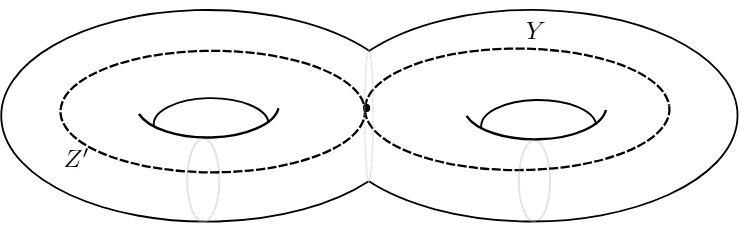
\includegraphics[width=0.5\linewidth]{../Graphics/2022AI1.png}
		\caption{Let $Y$ be the surface of genus 2, $Z$ the region bounded by $Y$ in $\mathbb{R}^3$, and $Z' \subset Y$ a loop that around each of handle of the handlebody.}
		\label{fig:2022AI1}
	\end{figure}
	
	We note that $Z$ deformation retracts onto $Z'$ (which can be seen by thinning out the handles of $Z$), and thus induces an isomorphism on fundamental groups; i.e., $\pi_{1}(Z, \text{pt}) \cong \pi_{1}(Z', \text{pt})$. On the other hand, since $Z' \subset Y$, $\pi_1(Z', \text{pt}) \subset \pi_{1}(Y, \text{pt})$. Thus, the inclusion homomorphism is surjective. Moreover, we now know that $\pi_{1}(Z, \text{pt}) \cong \mathbb{Z} \ast \mathbb{Z}$, which is a nonabelian group. Since the homomorphic image of an abelian group must necessarily be abelian, we conclude that $\pi_{1}(Y, \text{pt})$ must be nonabelian. 
	
	\begin{prb}{2022-A-I-4}
		Find the fundamental group of the space of unordered pairs of distinct points of $S^n$. 
	\end{prb}
	The space of unordered pairs of distinct points of $S^n$ deformation retracts onto the space of unordered pairs of antipodal points of $S^n$ (i.e., we can homotope distinct points so that they are diametrically opposite). Then one sees that this space is homotopy equivalent to the real projective space, $\mathbb{RP}^n$. Therefore, we conclude that 
	\begin{equation*}
		\pi_1(X) \cong \pi_1(\mathbb{RP}^n) \cong 
		\begin{cases}
			0, & n= 0 \\
			\mathbb{Z}, & n = 1, \\
			\mathbb{Z}/2\mathbb{Z}, & n \geq 2. 
		\end{cases}
	\end{equation*}
	
	\begin{prb}{2022-J-II-1}
		Let $M$ be a smooth connected manifold. Show that $M$ has a 2-fold cover $\ti{M}$ which is an orientable smooth manifold. What can you say about $\pi_0(\ti{M})$ if $M$ is not orientable? 
	\end{prb}
	Let $M$ be a smooth connected manifold. Essentially, we have to construct the orientation cover for $M$, which we will do as follows. Define 
	\begin{equation*}
		\ti{M} = \{(p, \mathcal{O}_{p}): p \in M \text{ and } \mathcal{O}_{p} \text{ is an orientation of $T_pM$}\}. 
	\end{equation*}
	Define the projection map $\hat{\pi}: \ti{M} \to M$ which sends an orientation of $T_pM$ to the point $p$ itself (i.e., $\hat{\pi}(p,\mathcal{O}_{p}) = p$). Since each tangent space has exactly two orientations, each fiber of this map has cardinality exactly 2. We will now show that $\hat{\pi}$ is a generalized covering map. For each pair $(U, \mathcal{O})$, where $U$ is an open subset of $M$ and $\mathcal{O}$ is an orientation for $U$, define a subset $\hat{U}_{\mathcal{O}} \subset \ti{M}$  as follows: 
	\begin{equation*}
		\hat{U}_{\mathcal{O}} = \{(p, \mathcal{O}_{p}) \in \ti{M}: p \in U \text{ and $\mathcal{O}_{p}$ is the orientation of $T_pM$ determined by $\mathcal{O}$}\}. 
	\end{equation*}
	Consider now an arbitrary point $(p,\mathcal{O}_{p}) \in \ti{M}$, and let $U$ be an orientable neighborhood of $p$ in $M$, and let $\mathcal{O}$ be an orientation on it. By replacing $\mathcal{O}$ by $-\mathcal{O}$ if necessary, we may assume that the given orientation $\mathcal{O}_{p}$ is the same as the orientation of $T_pM$ determined by $\mathcal{O}$. Thus, $(p, \mathcal{O}_{p}) \in \hat{U}_{\mathcal{O}}$. This shows that the collection of all sets of the form $\hat{U}_{\theta}$ covers $\ti{M}$. Now let $V$ be the component of $U \cap U'$ containing $p$. Then the restricted orientations $\mathcal{O}_{V}$ and $\mathcal{O}'_{V}$ agree at $p$, and therefore are identical. Therefore, $\hat{U}_{\mathcal{O}} \cap \hat{U}'_{\mathcal{O}}$ contains the basis set $\hat{V}_{\mathcal{O}\mid_V}$. Therefore, we have constructed a topology on $\ti{M}$. Note that for each orientable open subset $U \subseteq M$ and each orientation $\mathcal{O}$ of $U$, $\hat{\pi}$ maps the basis set $\hat{U}_{\mathcal{O}}$ bijectively onto $U$. Thus $\hat{\pi}$ is a local homeomorphism. 
	
	Now suppose that $U \subseteq M$ is an orientable connected open subset and $\mathcal{O}$ is an orientation for $U$. Then $\hat{\pi}^{-1}(U)$ is the disjoint union of open subsets $\hat{U}_\mathcal{O}$ and $\hat{U}_{-\mathcal{O}}$, and $\hat{\pi}$ restricts to a homeomorphism from each of these sets to $U$ Therefore, each such set $U$ is evenly covered, which shows that $\hat{\pi}$ is a generalized covering map. On each component of $\ti{M}$, $\hat{\pi}$ restricts to an ordinary covering map, and so each such component is a topological $n$-manifold and has a unique smooth structure making $\hat{\pi}$ into a smooth covering map. This induces a smooth structure on $\ti{M}$. 
	
	Now we will show that $\ti{M}$ is orientable. Let $\hat{p} = (p, \mathcal{O}_{p})$ be a point in $\ti{M}$. By definition, $\mathcal{O}_{p}$ is an orientation of $T_p M$, so that we can give $T_{\hat{p}}\ti{M}$ the unique orientation $\hat{\mathcal{O}}_{\hat{p}}$ such that $d\hat{\pi}_{\hat{p}}: T_{\hat{p}}\ti{M} \to T_p M$is orientation-preserving. This defines a pointwise orientation on $\ti{M}$. On each basis open subset $\hat{U}_{\mathcal{O}}$, the orientation $\hat{\mathcal{O}}$ agrees with the pullback orientation induced from $(U, \mathcal{O})$ by $\hat{\pi}$, so it is continuous. Thus, we have shown that $M$ has a 2-fold cover $\ti{M}$ which is an orientable smooth manifold. Now note that $|\pi_0(\ti{M})|$ is equivalent to the number of connected components of $\ti{M}$. If $M$ is not orientable, then we claim that $\ti{M}$ is connected. If $\ti{M}$ were not connected, a connected component would map diffeomorphically onto $M$ and thus choose a global orientation on $M$. Therefore, since $\ti{M}$ is connected, we conclude that $\pi_0(\ti{M})$ is trivial. 
	
	\begin{prb}{2022-J-II-5}
		Let $X \subset \mathbb{R}^{3}$ be the subspace consisting of the unit sphere $S^2$ and 5 parallel lines passing through the sphere (each intersecting the sphere at two points). Compute the fundamental group of $X$. 
	\end{prb}
	(Intuitive): Let $X$ subset $\mathbb{R}^{3}$ be the subspace consisting of the unit sphere $S^2$ and 5 parallel lines passing through the sphere (each intersecting the sphere at two points). The unbounded components of these lines deformation retract onto $S^2$ so that $X$ is homotopy equivalent to the space consisting of $S^2$ and five chords on $S^2$. We can homotope each of the intersection points to obtain the space that is the wedge sum of $S^2$ with $5$ loops; i.e., $X$ is homotopy equivalent to $S^{2} \vee S^1 \vee S^1 \vee S^1 \dotsm \vee S^1$. This means that 
	\begin{equation*}
		\pi_1(X) \cong \pi_{1}(S^{2}) \ast \underbrace{\pi_{1}(S^1) \ast \dotsm \ast \pi_{1}(S^1)}_{5 \text{ times}} \cong 0 \ast F_5 \cong F_5, 
	\end{equation*}
	where $F_5$ is the free group on 5 generators. 
	
	(Rigorous): Let $L_1, \dots, L_5 \subset \mathbb{R}^3$ be 5 distinct parallel lines intersecting $S^2$ at pairs of points $\{p_i, q_i\}$ for $i = 1, \dots, 5$, and let $X = S^2 \cup \left(\bigcup_{i=1}^5 L_i\right) \subset \mathbb{R}^3$.
	
	Each line $L_i$ is partitioned by $\{p_i, q_i\}$ into two unbounded rays $R_{i,1}, R_{i,2}$ and one bounded closed interval (chord) $I_i \cong [0, 1]$. Define $Y = S^2 \cup \left(\bigcup_{i=1}^5 I_i\right)$. Each ray $R_{i,j}$ is homeomorphic to $[0, \infty)$ anchored at $S^2$, so contracting each ray along its length to its endpoint defines a global deformation retraction of $X$ onto $Y$. Thus, the inclusion map $Y \hookrightarrow X$ is a homotopy equivalence, so $X \simeq Y$.
	
	Equip $S^2$ with its standard CW-structure. Attaching the 1-cells $I_i$ along their boundaries $\partial I_i = \{p_i, q_i\}$ yields a finite CW-complex structure on $Y$. Let $A = \bigcup_{i=1}^5 I_i$. Since each chord $I_i$ is a contractible 1-cell subcomplex, the pair $(Y, A)$ is a good pair (in the sense that $A$ is a closed subcomplex of the CW-complex $Y$). By the quotient theorem for good pairs with contractible components, the natural quotient map
	
	$$q: Y \longrightarrow Y / A$$
	
	is a homotopy equivalence, so $Y \simeq Y / A$.
	
	The quotient space $Y / A$ collapses each chord $I_i$ to a point, identifying the endpoints $p_i \sim q_i$ on $S^2$ for each $i = 1, \dots, 5$. Identifying $n$ pairs of distinct points on $S^2$ is homotopy equivalent to wedging $n$ copies of $S^1$ onto $S^2$. Therefore,
	
	$$Y / A = S^2 / \{p_1 \sim q_1, \dots, p_5 \sim q_5\} \ \simeq \ S^2 \vee \bigvee_{i=1}^5 S^1$$
	
	Since homotopy equivalences preserve fundamental groups, we have
	
	$$\pi_1(X) \cong \pi_1(Y) \cong \pi_1(Y / A) \cong \pi_1\left(S^2 \vee \bigvee_{i=1}^5 S^1\right)$$
	
	Thus, we conclude that
	
	$$\pi_1(X) \cong \pi_1(S^2) * \underbrace{\pi_1(S^1) * \dots * \pi_1(S^1)}_{5 \text{ times}} \cong \{e\} * \underbrace{\mathbb{Z} * \dots * \mathbb{Z}}_{5 \text{ times}} \cong F_5$$
	
	where $F_5$ is the free group on 5 generators.
	
	\begin{prb}{2022-J-II-5 (Modified)}
		Let $X \subset \mathbb{R}^{3}$ be the subspace consisting of the 2-torus $T$ and a line passing through $T$ (intersecting the torus at $n > 1$ points). Compute the fundamental group of $X$. 
	\end{prb}
	There are three possible cases: $n = 2, 3$, or $4$ as indicated in Figure \ref{fig:2022JII5}.
	\begin{figure}[h!]
		\centering 
		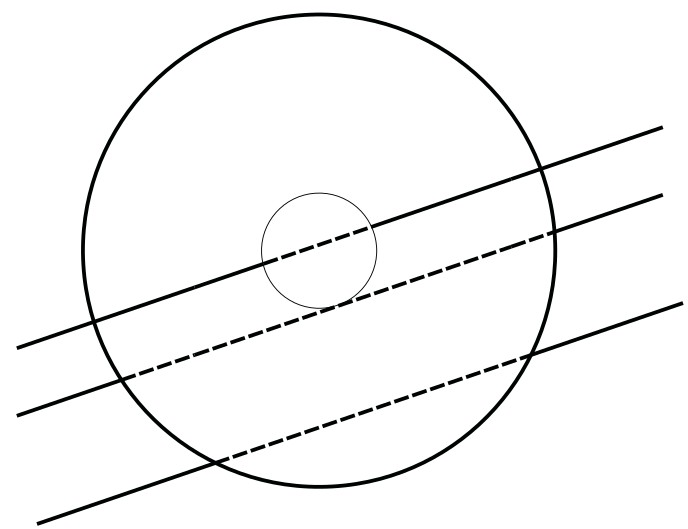
\includegraphics[scale =0.4]{../Graphics/2022JII5.jpg}
		\caption{Top view of $T$ with intersecting lines. From bottom to top: case 1 to case 3.}
		\label{fig:2022JII5}
	\end{figure}
	\begin{enumerate}[itemsep =-2pt,label = (\arabic{*})]
		\item ($n = 2$): Let $L \subset \mathbb{R}^{3}$ denote the line that passes through $T$ at exactly 2 points $p$ and $q$; set $X = T \cup L$. We note that $L$ has three components: (1) two unbounded rays $R_1$ and $R_2$ that are each homeomorphic to $[0,\infty)$, and (2) one closed bounded interval $I_1 \simeq [0,1]$; set $Y = T \cup I_1$. We note that each ray deformation retracts onto its endpoints so that $X \simeq Y$. Now assign $T$ its standard CW structure (composed of one 0-cell, two 1-cells, and one 2-cell), and attach the 1-cell $I_1$ to its boundary $\partial I_1 = \{p, q\}$. This gives $Y$ a finite CW complex structure. Since $I_1$ is a contractible 1-cell subcomplex, the pair $(Y, I_1)$ is a good pair in the sense that $I_1$ is a closed subcomplex of the CW-complex $Y$. Therefore, one has that $Y\simeq Y/I_1$. The quotient space $Y/I_1$ collapses $I_1$ to a point, identifying the endpoints $p \sim q$ on $T$. Since identifying a pair on $T$ is homotopy equivalent to wedging a copy of $S^1$ onto $S^2$, one has that $Y \simeq T \vee S^1$. Therefore, we conclude that 
		\begin{equation*}
			\pi_1(X) \cong \pi_1(Y) \cong \pi_{1}(T \vee S^1) \cong \pi_1(T) \ast \pi_1(S^1) \cong (\mathbb{Z} \times \mathbb{Z}) \ast \mathbb{Z} = \braket{a, b, c\mid aba^{-1}b^{-1} = 1}. 
		\end{equation*}
		\item ($n = 2$): Let $L \subset \mathbb{R}^3$ denote the line that passes through $T$ at exactly 3 points $p, q$, and $r$; set $X = T \cup L$. We note that $L$ has four components: (1) two unbounded rays $R_1, R_2$, each homeomorphic to $[0,\infty)$, and (2) two closed bounded intervals $I_1$ and $I_2$, each homeomorphic to $[0,1]$. Set $Y = T \cup I_1 \cup I_2$. We note that the unbounded rays $R_1$ and $R_2$ deformation retract onto their endpoints so that $X \simeq Y$. Set $A = I_1 \cup I_2$. Give $T$ its standard CW structure (i.e., one 0-cell, two 1-cells, and one 2-cell), and attach the 2 1-cells $I_1, I_2$ to their respective boundaries ($\{p, q\}$ and $\{q, r\}$). This gives $Y$ a finite CW complex structure. Since $A$ is a contractible 1-cell subcomplex, $(Y, A)$ forms a good pair so that $Y \simeq Y/A$. The quotient space $Y/A$ collapses each cord into a single point, thus identifying the endpoints $p \sim q \sim r$ on $T$. This is homotopy equivalent to wedging two copies of $S^1$ onto $T$; i.e., $Y \simeq T \vee S^1 \vee S^1$. Therefore, we conclude that 
		\begin{equation*}
			\pi_1(T) \cong (\mathbb{Z} \times \mathbb{Z}) \ast F_2 \cong \braket{a, b, c, d \mid aba^{-1}b^{-1} = 1}. 
		\end{equation*}
		\item ($n = 4$) Generalizing the two arguments from above, one concludes that 
		\begin{equation*}
			\pi_1(X) \cong (\mathbb{Z} \times \mathbb{Z}) \ast F_{3} \cong \braket{a, b, c, d, f \mid aba^{-1}b^{-1} = 1}. 
		\end{equation*}
	\end{enumerate}
	
	\begin{prb}{2021-A-II-3}
		Let $X$ be the space obtained by gluing the boundary circle of a M\"obius band to a great circle in $S^{2}$. Compute the fundamental group of $X$. 
	\end{prb}
	Let $X$ be the space obtained by gluing the boundary circle of the M\"obius band to a great circle (e.g., the equator) in $S^{2}$. We can compute the fundamental group of $X$ using CW structures. Let $S^2$ have the CW structure consisting of one $0$-cell $v$, one $1$-cell $e_C^1$ (the equator), and two $2$-cells $e_N^2,e_S^2$ attached along $e_C^1$. Thus
	\begin{equation*}
		\pi_1(S^2)\cong \langle e_C^1 \mid e_C^1 = 1 \rangle.
	\end{equation*}
	Let $M$ denote the Möbius band. Since $M$ deformation retracts onto its core circle,
	\begin{equation*}
		\pi_1(M)\cong \langle a \rangle \cong \mathbb{Z},
	\end{equation*}
	where $a$ is represented by the core circle. Under this deformation retraction, the boundary circle of $M$ wraps twice around the core circle, so its image in $\pi_1(M)$ is $a^2$. Gluing $\partial M$ to the equator of $S^2$ identifies the loop $e_C^1$ with $a^2$. By Seifert--van Kampen,
	\begin{equation*}
		\pi_1(X)
		\cong
		\langle e_C^1,a \mid e_C^1 = 1,\ e_C^1 = a^2 \rangle
		\cong
		\langle a \mid a^2 = 1 \rangle
		\cong
		\mathbb{Z}/2\mathbb{Z}.
	\end{equation*}
	
	\begin{prb}{2021-A-II-3 (Modified)}
		Let $X$ be the space obtained by gluing the boundary circle of a M\"obius band to the equator of the 2-torus. Compute the fundamental group of $X$. 
	\end{prb}
	Let $X$ be the space obtained by gluing the boundary circle of the Möbius strip to the equator of the 2-torus. We can compute the fundamental group of $X$ using CW structures. We assign to $T^{2}$ the standard CW structure comprised of one 0-cell $v$, two 1-cells $e^{1}_{C}, e^{1}_{R}$ (where $e^{1}_{C}$ corresponds to the equator of the 2-torus), and one 2-cell $e^{2}_{T}$; $\partial e^{2}_{T}$ attaches to the 1-skeleton along the boundary word $e^{1}_{R}e^{1}_{C}(e^{1}_{R})^{-1}(e^{1}_{C})^{-1}$. This means that the fundamental group of the torus is $\langle e^{1}_{C}, e^{1}_{R} \mid [e^{1}_{C}, e^{1}_{R}] = 1 \rangle$. Next, since the Möbius band deformation retracts onto its core circle $a$, $\pi_{1}(M) \cong \langle a \rangle \cong \mathbb{Z}$. Under this deformation retraction, the boundary circle of the Möbius band wraps around the core circle $a$ twice so that its image in $\pi_{1}(M)$ is $a^{2}$. By gluing the boundary circle of the band to the equator of the 2-torus, we identify $e^{1}_{C}$ with $a^{2}$. Thus by the Seifert–van Kampen theorem, we conclude that
	\begin{equation*}
		\pi_{1}(X) \cong \langle e^{1}{C}, e^{1}{R}, a \mid [e^{1}{C}, e^{1}{R}] = 1, e^{1}{C} = a^{2} \rangle \cong \langle a, e^{1}{R} \mid [a^{2}, e^{1}_{R}] = 1 \rangle.
	\end{equation*}
	
	\begin{prb}{2021-A-II-3 (Modified)}
		Let $X$ be the space obtained by gluing the equator of the 2-torus to the equator of the 2-sphere. Compute the fundamental group of $X$. 
	\end{prb}
	Let $X$ be the space obtained by gluing the equator of the 2-torus to the equator of the 2-sphere. We can compute the fundamental group of $X$ using CW structures. Let $S^{2}$ have the CW structure comprised of one 0-cell $v$, one 1-cell $e^{1}_{S}$ (corresponding to the equator), and two 2-cells $e^{2}_{N}$ and $e^{2}_{S}$ (corresponding to the northern and southern hemispheres, respectively). These 2-cells are both attached to the 1-cell $e^{1}_{S}$. Now we give the 2-torus the CW structure comprised of one 0-cell, two 1-cells $e^{1}_{C}$ and $e^{1}_{R}$ (where $e^{1}_{C}$ denotes the equator circle), and one 2-cell $e^{2}_{T}$. $\partial e^{2}_{T}$ is attached to the 1-skeleton of the 2-torus along the boundary word $e^{1}_{R}e^{1}_{C}(e^{1}_{R})^{-1}(e^{1}_{C})^{-1}$. We identify the 0-cell in the 2-torus to the 0-cell $v$ in the CW structure of the 2-sphere. The gluing identifies the loop $e^{1}_{S}$ with the loop $e^{1}_{C}$. Thus, by the Seifert-van Kampen theorem, we conclude that 
	\begin{equation*}
		\pi_{1}(X) \cong \braket{e^{1}_{C}, e^{1}_{R}, e^{1}_{S} \mid [e^{1}_{C}, e^{1}_{R}] = 1, e^{1}_{S} = 1,  e^{1}_{C} = e^{1}_{S}} \cong \braket{e^{1}_{R}} \cong \mathbb{Z}. 
	\end{equation*}
	
	Alternately, let $U \subseteq X$ denote the open subset comprised of the 2-torus $T$ and a small band in the 2-sphere $S^2$ around the equator. Likewise, let $V$ denote the open subset comprised of $S^2$ and a small band in $T$ around the equator. Then $U$ deformation retracts onto $T$, while $V$ deformation retracts onto $S^2$. Moreover, $U \cap V$ deformation retracts onto the equator circle $\gamma$ so that $\pi_{1}(U \cap V) \cong \braket{\gamma} \cong \mathbb{Z}$. Let $i_{1}: U \cap V \hookrightarrow U$ and $i_{2}: U \cap V \hookrightarrow V$ denote the standard inclusion maps, and let $i_{1,\ast}$ and $i_{2,\ast}$ be the respective induced maps on the fundamental groups. Since $S^{2}$ is simply connected, $\pi_{1}(V)$ is trivial so that $i_{2,\ast}$ is the trivial map. On the other hand, $\pi_{1}(T) \cong \braket{a, b \mid [a,b]= 1} \cong \mathbb{Z}^{2}$, where $a$ is the equator circle of the 2-torus. By gluing the equator of the 2-torus to the equator of the 2-sphere, we identify $\gamma$ with $a$. Therefore, by the Seifert-van Kampen Theorem, we conclude that 
	\begin{equation*}
		\pi_{1}(X) \cong \pi_{1}(U) \ast_{\pi_{1}(U \cap V)} \pi_{1}(V) \cong \braket{a, b \mid [a, b] = 1, i_{1, \ast}(\gamma) = i_{2,\ast}(\gamma)} = \braket{a , b \mid a = 1} \cong \braket{b} \cong \mathbb{Z}. 
	\end{equation*}
	
	\begin{prb}{2021-J-I-2}
		Define an equivalence relation $\sim$ on the 2-dimensional torus $S^{1} \times S^{1}$ as follows: $(x, y) \sim (u, v)$ iff either $(x, y)= (u, v)$ or $(x, y) = (v, u)$. Compute the fundamental group for the quotient space $(S^{1}\times S^{1})/\sim$ and describe the universal cover for this space. 
	\end{prb}
	Represent $T^2$ as $[0,1]^2 / \sim_{T^2}$. The swap action $(x,y) \mapsto (y,x)$ restricts $T^2$ to the fundamental domain given by the lower triangle $D = \{(x,y) \in [0,1]^2 \mid y \le x\}$. Under the combined torus and swap identifications, the bottom edge $(t,0)$ is glued head-to-tail to the right edge $(1,t)$ via $(t,0) \sim (1,t)$, while all three corner vertices collapse to a single basepoint $v$, and the diagonal $y=x$ forms an unglued boundary loop. Gluing two adjacent edges of a triangle head-to-tail yields a Möbius strip.
	
	Using $D$ to induce a CW structure on $X = T^2 / \sim$, we have one $0$-cell $v$, two $1$-cells $a$ (the diagonal loop) and $b$ (the glued legs loop), and one $2$-cell attached along the boundary word $b^2 a^{-1}$. By the cell-attachment theorem, $\pi_1(X) \cong \langle a, b \mid b^2 a^{-1} = 1 \rangle \cong \langle b \mid \varnothing \rangle \cong \mathbb{Z}$. Because $X$ is homeomorphic to the Möbius strip, its fundamental group is $\mathbb{Z}$, and its universal cover is the contractible 2-manifold with boundary given by the infinite strip $\mathbb{R} \times [-1, 1]$ equipped with the standard covering map under the deck transformation group $\mathbb{Z}$ generated by the glide reflection $(x, y) \mapsto (x+1, -y)$. Visually, the construction is outlined in Figure \ref{fig:2021JI2}
	\begin{figure}[h!]
		\centering 
		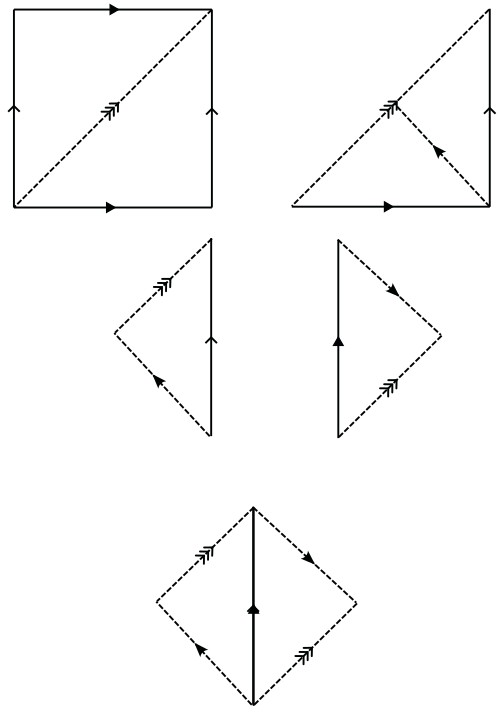
\includegraphics[width = 0.4\textwidth]{../Graphics/2021JI2.jpg}
		\label{fig:2021JI2}
	\end{figure}
	
	\begin{prb}{2020-A-II-2}
		Let $X$ be the ``figure eight,'' i.e., the wedge of two circles joined at a point $x_{0} \in X$. Recall that the fundamental group $G = \pi_{1}(X,x_{0})$ is the free group on two generators $a, b$ running once along each of the circles. Let $H \leq G$ be the subgroup generated by $a$, $bab^{-1}$, and $b^{2}$. Draw the covering space of $X$ corresponding to $H$, and show that $H$ is isomorphic to a free group on the three given generators. 
	\end{prb}
	First, we will determine the cosets in the quotient $G/H$; let $H = \braket{a, bab^{-1}, b^{2}}$. The coset $aH$ is equivalent to the coset $H$ since $a \in H$. Likewise, $bab^{-1}H$ and $b^{2}H$ are both equal to $H$. On the other hand, define the group homomorphism $\phi: F(a,b) \to \mathbb{Z}_2$ by sending: $$\phi(a) = 0 \pmod 2, \quad \phi(b) = 1 \pmod 2.$$ Evaluating $\phi$ on the generators of $H$: (1) $\phi(a) = 0$, (2) $\phi(bab^{-1}) = 1 + 0 - 1 \equiv 0 \pmod 2$, and (3) $\phi(b^2) = 1 + 1 \equiv 0 \pmod 2$. Since $\phi$ vanishes on all generators of $H$, we have $H \subseteq \ker(\phi)$. Every word in $H$ must have an even total exponent sum in $b$. However, $\phi(b) = 1 \neq 0$, so $b \notin \ker(\phi) \implies b \notin H$. Thus, the left coset $bH$ is distinct from $H$. Now we will show that $\{H, bH\}$ form the complete set of cosets of $H$. The action of $a$ and $b$ on $H$ give the cosets $H$ and $bH$. Likewise, the action of $a$ and $b$ on $bH$ give the cosets $abH = b(b^{-1}ab)H = bH$ since $b^{2}, bab^{-1} \in H$ implies $b^{-1}abH = H$, and $b^{2}H = H$. Thus since $\{H, bH\}$ is closed under left multiplication by $a, b, a^{-1}, b^{-1}$, there exist no other cosets of $H$. Therefore, since there are precisely 2 cosets of $G$, the covering space corresponding to $H$ is 2-sheeted, with each vertex corresponding to one of the cosets. The directed edges are then given by the left action of the generators $a$ and $b$ on each coset. Since $a$ acts as the identity on the cosets, we obtain two directed $a$-edges, one loop at each vertex. On the other hand, since $v_{0} = H \xrightarrow{b} v_{1} = bH$ and $v_{1} \xrightarrow{b} v_{0}$, we get two directed $b$-edges, one from $v_{0}$ to $v_{1}$, and the other from $v_{1}$ to $v_{0}$. Thus we conclude with the following drawing. Looking at point $p$ shows the three free generators.
	\begin{figure}[h!]
		\centering 
		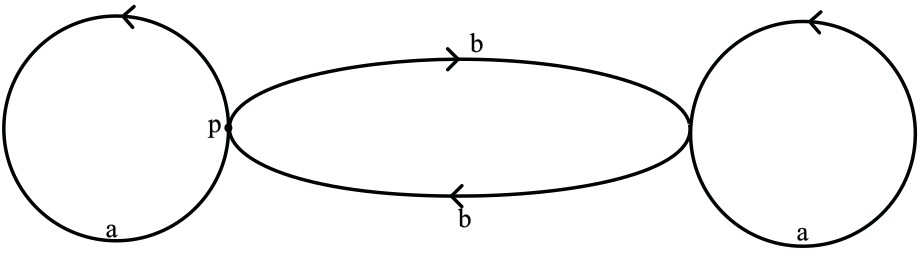
\includegraphics[width = 0.44\textwidth]{../Graphics/2020AII2.jpg}
	\end{figure}
	
	\begin{prb}{2018-A-II-1}
		Let $B$ denote the M\"obius band, and let $\partial B$ denote its boundary, which arises from the top and bottom line segments. Show that there is no retraction mapping $r: B \to \partial B$. 
	\end{prb}
	Let $B$ denote the M\"obius band, and let $\partial B$ denote its boundary. Assume to the contrary that there exists a retraction mapping $r: B \to \partial B$. This means that if $\iota: \partial B \hookrightarrow B$ denotes the standard inclusion map, then $r \circ \iota = \operatorname{id}_{\partial B}$. In particular, one has that $r_{\ast} \circ \iota_{\ast} = \operatorname{id}_{\partial B\ast}$. The boundary $\partial B$ is a topological circle so that $\pi_{1}(\partial B) = \braket{[\gamma]} \cong \mathbb{Z}$, where $\gamma$ denotes the boundary loop. Note that $[\gamma] \neq [0]$. Let $a$ denote the core circle of $B$; since $B$ deformation retracts onto $a$, one has that $\pi_{1}(M) \cong \braket{[a]} \cong \mathbb{Z}$. Since the boundary circle $\gamma$ loops around the core circle twice, $\iota_{\ast}([\gamma]) = 2[a]$. Next since $r_{\ast}$ is surjective, it follows that $r_{\ast}([a]) = n[\gamma]$ for some nonzero integer $n$. Therefore, 
	\begin{equation*}
		[\gamma] = \operatorname{id}_{\partial B\ast}([\gamma]) = r_{\ast} \circ \iota_{\ast}([\gamma]) = 2n[\gamma]. 
	\end{equation*}
	Since $[\gamma] \neq [0]$, one must have $2n = 0 \iff n = 0$, which then implies $r_{\ast}$ is the trivial homomorphism (and therefore, is not surjective since $\pi_{1}(\partial B)$ is nontrivial). This is a contradiction! Thus by contradiction, there cannot be a retraction mapping $r: B \to \partial B$. 
	
	\begin{prb}{2012-A-II-3}
		Prove that every smooth, connected manifold whose fundamental group has finite, odd order is an orientable manifold. 
	\end{prb}
	Let $M$ be a smooth, connected manifold whose fundamental group has finite, odd order. Let $\hat{M}$ denote the orientation cover on $M$, and let $p: \hat{M} \to M$ denote the covering map. Since $p$ is a covering map, one has that $p_{\ast}: \pi_1(\hat{M}, x_0) \to \pi_1(M, p(x_0))$ is injective, and thus $p_\ast(\pi_1(\hat{M}, x_0)) \leq \pi_1(M, p(x_0))$. If $M$ is \textit{not} orientable (i.e., $\hat{M}$ is a connected space), then since $p$ is a 2-sheeted covering space, $p_\ast(\pi_1(\hat{M}, x_0))$ must be an index-2 subgroup of $\pi_1(M,p(x_0))$. By Lagrange's theorem, it follows that $2$ is a divisor of the order of the fundamental group of $M$, so that it has even order. This is a contradiction! Thus by contradiction, $M$ must be orientable. 
	
	\begin{prb}{2011-A-I-5}
		A map $f: X \to Y$ between two topological spaces is said to be proper if $f^{-1}(K) \subset X$ is compact whenever $K \subset Y$ is compact. Let $M$ be a connected manifold, and $p: \ti{M} \to M$ be its universal cover. Show that $p$ is a proper map if and only if $M$ has finite fundamental group. 
	\end{prb}
	Let $M$ be a connected manifold, and $p: \ti{M} \to M$ be its universal cover. 
	
	($\Longleftarrow$) We start by assuming that $M$ has finite fundamental group. This means that $p_{\ast}(\pi_{1}(\ti{M}, x_0)) \subseteq \pi_1(M, p(x_0))$ must be a finite subgroup. Thus, $p$ must be a finite $k$-sheeted covering map. Let $K \subseteq M$ be an arbitrary compact subset of $M$, and let $\{W_{\alpha}\}$ be an arbitrary open cover of $p^{-1}(K)$. Fix an arbitrary $q \in K$, and assume that $p^{-1}(q) = \{e_1, \ldots, e_k\}$. Then since the $W_\alpha$ cover $p^{-1}(K)$, there exist $W_{\alpha_1}, \ldots, W_{\alpha_k}$ such that for each $j = 1, \ldots, k$, $e_j \in W_{\alpha_j}$. We also know by the definition of a covering space that there exists an evenly covered neighborhood $W_q$ of $q$ in $M$. Let $p^{-1}(W_q) = \bigsqcup_{1}^{k}V_{j}$, where each $V_j$ is an open subset of $\ti{M}$ and $p: V_j \to W_q$ is a homeomorphism. In particular, $p(V_j \cap W_{\alpha_j})$ is an open neighborhood of $q$ in $M$ for each $j$. So now define, 
	\begin{equation*}
		\ti{U}_{q} \coloneqq \bigcap_{1}^{k}p(V_j \cap W_{\alpha_j}), 
	\end{equation*}
	which is an open neighborhood of $q$ in $M$. Consider the collection $\{\ti{U}_{q}\}_{q\in K}$, where for each $q \in K$, $\ti{U}_q$ is defined above; this collection is an open cover of $K$. Thus there exists a finite subcover $\{\ti{U}_{q_j}\}_{j = 1}^{n}$ of $K$. For each $j$, one has 
	\begin{equation*}
		p^{-1}(\ti{U}_{q_{j}}) = \bigsqcup_{l = 1}^{k}V_{j,l}, 
	\end{equation*}
	where $V_{j,l} \coloneqq V_l \cap p^{-1}(\ti{U}_{q_j})$. By construction of $\ti{U}_{q_j}$, we have $V_{j,l} \subset W_{\alpha_l}^j$. Thus we have a finite subcollection (of $nk$) open subsets $\{W_{\alpha_l}^{j}: j = 1, \ldots, n, l = 1, \ldots, k\}$, and 
	\begin{align*}
		\begin{split}
			p^{-1}(K) &= p^{-1}\left(\bigcup_{j = 1}^{n}\ti{U}_{q_{j}}\right) = \bigcup_{j = 1}^{n}p^{-1}(\ti{U}_{q_j}) \\
			&= \bigcup_{j = 1}^{n}\left(\bigsqcup_{l = 1}^{k}V_{j,l}\right) \subset \bigcup_{j = 1}^{n}\bigcup_{l = 1}^{k}W_{\alpha_{l}}^{j}. 
		\end{split}
	\end{align*}
	Thus since an arbitrary open cover of $p^{-1}(K)$ admits a finite open subcover, $p^{-1}(K)$ is compact. Since $K$ was arbitrary, we conclude that $p$ is proper. 
	
	($\Longrightarrow$) Now assume that $p$ is a proper map. Then since for each $p \in M$, $\{p\}$ is compact, $p^{-1}(\{q\})$ is discrete (since $q$ has an evenly covered neighborhood) and is compact. Thus since $\ti{M}$ is Hausdorff, $p^{-1}(q)$ is finite. Since this is true for every $q \in M$, $p$ is a finite-sheeted covering space. Now since $M$ admits a universal covering space, $\pi_{1}(M) \cong \Gamma$, where $\Gamma$ is the group of deck transformations. In particular, since the cardinality of the group of deck transformations is equal to the number of sheets, $|\pi_1(M)| = |p^{-1}(q)| < \infty$. Thus the proof concludes.
	
	\begin{prb}{2010-A-I-3}
		Let $X$ be the topological subspace of $\mathbb{R}^3$ consisting of the unit sphere $S^2$ and $5$ parallel lines passing through the sphere (each intersecting $S^2$ at 2 points.) Compute $\pi_1(X)$. 
	\end{prb}
	Let $L_1, \dots, L_5 \subset \mathbb{R}^3$ be 5 distinct parallel lines intersecting $S^2$ at pairs of points $\{p_i, q_i\}$ for $i = 1, \dots, 5$, and let $X = S^2 \cup \left(\bigcup_{i=1}^5 L_i\right) \subset \mathbb{R}^3$.
	
	Each line $L_i$ is partitioned by $\{p_i, q_i\}$ into two unbounded rays $R_{i,1}, R_{i,2}$ and one bounded closed interval (chord) $I_i \cong [0, 1]$. Define $Y = S^2 \cup \left(\bigcup_{i=1}^5 I_i\right)$. Each ray $R_{i,j}$ is homeomorphic to $[0, \infty)$ anchored at $S^2$, so contracting each ray along its length to its endpoint defines a global deformation retraction of $X$ onto $Y$. Thus, the inclusion map $Y \hookrightarrow X$ is a homotopy equivalence, so $X \simeq Y$.
	
	Equip $S^2$ with its standard CW-structure. Attaching the 1-cells $I_i$ along their boundaries $\partial I_i = \{p_i, q_i\}$ yields a finite CW-complex structure on $Y$. Let $A = \bigcup_{i=1}^5 I_i$. Since each chord $I_i$ is a contractible 1-cell subcomplex, the pair $(Y, A)$ is a good pair (in the sense that $A$ is a closed subcomplex of the CW-complex $Y$). By the quotient theorem for good pairs with contractible components, the natural quotient map
	
	$$q: Y \longrightarrow Y / A$$
	
	is a homotopy equivalence, so $Y \simeq Y / A$.
	
	The quotient space $Y / A$ collapses each chord $I_i$ to a point, identifying the endpoints $p_i \sim q_i$ on $S^2$ for each $i = 1, \dots, 5$. Identifying $n$ pairs of distinct points on $S^2$ is homotopy equivalent to wedging $n$ copies of $S^1$ onto $S^2$. Therefore,
	
	$$Y / A = S^2 / \{p_1 \sim q_1, \dots, p_5 \sim q_5\} \ \simeq \ S^2 \vee \bigvee_{i=1}^5 S^1$$
	
	Since homotopy equivalences preserve fundamental groups, we have
	
	$$\pi_1(X) \cong \pi_1(Y) \cong \pi_1(Y / A) \cong \pi_1\left(S^2 \vee \bigvee_{i=1}^5 S^1\right)$$
	
	Thus, we conclude that
	
	$$\pi_1(X) \cong \pi_1(S^2) * \underbrace{\pi_1(S^1) * \dots * \pi_1(S^1)}_{5 \text{ times}} \cong \{e\} * \underbrace{\mathbb{Z} * \dots * \mathbb{Z}}_{5 \text{ times}} \cong F_5$$
	
	\begin{prb}{2009-A-I-4}
		Let $M$ be a smooth, connected manifold whose fundamental group contains at least three distinct elements. If $\pi_1(M)$ is a simple group, prove that $M$ is an orientable manifold. 
	\end{prb}
	Let $M$ be a smooth, connected manifold whose fundamental group contains at least three distinct elements. Further assume that $\pi_1(M)$ is a simple group. Let $\hat{M}$ be the orientation cover of $M$, and let $\hat{p}: \hat{M} \to M$ denote the covering map; $\hat{p}_{\ast}: \pi_1(\hat{M}, x_0) \to \pi_1(M, p(x_0))$ must be an injective map. Assume to the contrary that $M$ is non-orientable. Then since $\hat{p}$ is a 2-sheeted covering map, $p_\ast(\pi_1(\hat{M}, x_0))$ must be an index-2 subgroup of $\pi_1(M, p(x_0))$. Since any subgroup of index 2 is normal, $p_\ast(\pi_1(\hat{M}, x_0))$ is a normal subgroup of $\pi_1(M, p(x_0))$. Since this subgroup has index 2, it cannot be the entire group. On the other hand, it cannot be the trivial subgroup either (the index of the trivial subgroup is precisely $|\pi_1(M, p(x_0))| \geq 3$). Therefore, we have shown that $\pi_1(M, x_0)$ has a proper nontrivial normal subgroup, which contradicts our hypothesis that it is a simple group. Thus by contradiction, $M$ must be an orientable manifold. 
	
	\begin{prb}{2006-A-II-6}
		Let $X$ be the topological subspace of $\mathbb{R}^3$ consisting of the unit sphere $S^2$ and $5$ parallel lines passing through the sphere (each intersecting $S^2$ at 2 points.) Compute $\pi_1(X)$. 
	\end{prb}
	Let $L_1, \dots, L_5 \subset \mathbb{R}^3$ be 5 distinct parallel lines intersecting $S^2$ at pairs of points $\{p_i, q_i\}$ for $i = 1, \dots, 5$, and let $X = S^2 \cup \left(\bigcup_{i=1}^5 L_i\right) \subset \mathbb{R}^3$.
	
	Each line $L_i$ is partitioned by $\{p_i, q_i\}$ into two unbounded rays $R_{i,1}, R_{i,2}$ and one bounded closed interval (chord) $I_i \cong [0, 1]$. Define $Y = S^2 \cup \left(\bigcup_{i=1}^5 I_i\right)$. Each ray $R_{i,j}$ is homeomorphic to $[0, \infty)$ anchored at $S^2$, so contracting each ray along its length to its endpoint defines a global deformation retraction of $X$ onto $Y$. Thus, the inclusion map $Y \hookrightarrow X$ is a homotopy equivalence, so $X \simeq Y$.
	
	Equip $S^2$ with its standard CW-structure. Attaching the 1-cells $I_i$ along their boundaries $\partial I_i = \{p_i, q_i\}$ yields a finite CW-complex structure on $Y$. Let $A = \bigcup_{i=1}^5 I_i$. Since each chord $I_i$ is a contractible 1-cell subcomplex, the pair $(Y, A)$ is a good pair (in the sense that $A$ is a closed subcomplex of the CW-complex $Y$). By the quotient theorem for good pairs with contractible components, the natural quotient map
	
	$$q: Y \longrightarrow Y / A$$
	
	is a homotopy equivalence, so $Y \simeq Y / A$.
	
	The quotient space $Y / A$ collapses each chord $I_i$ to a point, identifying the endpoints $p_i \sim q_i$ on $S^2$ for each $i = 1, \dots, 5$. Identifying $n$ pairs of distinct points on $S^2$ is homotopy equivalent to wedging $n$ copies of $S^1$ onto $S^2$. Therefore,
	
	$$Y / A = S^2 / \{p_1 \sim q_1, \dots, p_5 \sim q_5\} \ \simeq \ S^2 \vee \bigvee_{i=1}^5 S^1$$
	
	Since homotopy equivalences preserve fundamental groups, we have
	
	$$\pi_1(X) \cong \pi_1(Y) \cong \pi_1(Y / A) \cong \pi_1\left(S^2 \vee \bigvee_{i=1}^5 S^1\right)$$
	
	Thus, we conclude that
	
	$$\pi_1(X) \cong \pi_1(S^2) * \underbrace{\pi_1(S^1) * \dots * \pi_1(S^1)}_{5 \text{ times}} \cong \{e\} * \underbrace{\mathbb{Z} * \dots * \mathbb{Z}}_{5 \text{ times}} \cong F_5.$$
	
	where $F_5$ is the free group on 5 generators.
	
	\begin{prb}{2004-A-II-6}
		Define a subset $X \subset \mathbb{R}^{3}$ by $X = \{(x, y, z) \in \mathbb{R}^{3}: x^{2} + y^{2} + z^{1} = 1\} \cup \{(0,0,z) \in \mathbb{R}^{3}: -1 \leq z \leq 1\}$. \vspace{-0.25cm}
		\begin{enumerate}[itemsep =-2pt,label = (\alph{*})]
			\item Use van Kampen's theorem to calculate $\pi_{1}(X)$. 
			\item Describe the universal cover $\ti{X}$ of $X$ and the covering map, and hence give a second calculation for $\pi_{1}(X)$. 
		\end{enumerate}
	\end{prb}
	Let $X$ be the space described above. \vspace{-0.25cm}
	\begin{enumerate}[itemsep = -2pt,label = (\alph{*})]
		\item $X$ is homotopy equivalent to the space $Y$ consisting of the 2-sphere $S^{2} \subset \mathbb{R}^{3}$ and an arc on $S^{2}$ connecting the north and the south poles. Since any such arc between the poles of $S^{2}$ is a contractible subcomplex, the space $Z$ obtained by collapsing such a subcomplex to a single point (i.e., by identifying the north and south poles) is homotopy equivalent to $Y$, and thus to $X$. But the space $Z$ is homotopy equivalent to the wedge sum $S^{2}\vee S^{1}$. Let $U$ be the open subset composed of $S^{2}$ and an open half of $S^{1}$, and $V$ be the open subset composed of $S^{1}$ and an open half of $S^{2}$. Then $U \cap V$ is contractible so that $\pi_{1}(U \cap V) = 0$. On the other hand $U \simeq S^{2}$ and $V \simeq S^{1}$ so that $\pi_{1}(U) \cong 0$ and $\pi_{1}(V) \cong \mathbb{Z}$. Thus by the Seifert-van Kampen theorem, since $U \cap V$ is simply connected, 
		\begin{equation*}
			\pi_{1}(X) \cong \pi_{1}(U) \ast_{\pi_{1}(U \cap V)} \pi_{1}(V) \cong \pi_{1}(V) \cong \mathbb{Z}. 
		\end{equation*}
		Alternately, since $S^{2}$ is simply connected, adding one such arc creates a loop and no relations so that by van Kampen, $\pi_{1}(X) \cong \mathbb{Z}$. 
		\item The universal cover $\ti{X}$ of $X$ is an infinite chain of copies of $S^{2}$, where consecutive copies of $S^{2}$ are joined together at the lifts of the intersection point to a lifted copy of the interval between the corresponding poles (i.e., consider the real line, with spheres attached to the line at equal intervals by only one point). If $p: \ti{X} \to X$ is the covering map, then on the real line, $p$ corresponds to the standard universal covering map $p: \mathbb{R} \to S^{1}$ given by $p(t) = e^{2p\pi i t}$. On each copy of $S^{2}$, $p$ maps homeomorphically onto $S^{2}$. The deck transformations are the homeomorphisms $\phi: \tilde{X} \to \tilde{X}$ satisfying $p \circ \phi = p$.These correspond to integer translations along the real line:$$\phi_k(t) = t + k, \quad \text{mapping } S^2_n \to S^2_{n+k} \text{ for } k \in \mathbb{Z}.$$ The deck transformation group $\Gamma$ is therefore isomorphic to $\mathbb{Z}$. Since $\pi_{1}(\ti{X})$ is easily seen to be trivial, it follows that $\pi_{1}(X) \cong \Gamma \cong \mathbb{Z}$. 
	\end{enumerate}
	
	\begin{prb}{2004-J-I-5}
		Recall that a connected sum $M \# N$ of two $n$-dimensional manifolds $M$, $N$ is constructed as follows: cut out the interior of a closed $n$-dimensional ball from each manifold, and glue the resulting spaces together along their $(n - 1)$-sphere boundaries. \vspace{-0.25cm} 
		\begin{enumerate}[itemsep =-2pt,label = (\alph{*})]
			\item Let $\mathbb{RP}^{n}$ denote the $n$-dimensional real projective space. If $n > 2$, then compute the fundamental group of the connected sum $\mathbb{RP}^{n} \#\mathbb{RP}^{n}$. 
			\item If $n > 2$, then show that the universal covering space for the connected sum $\mathbb{RP}^{n}\# \mathbb{RP}^{n}$ is homemorphic to the product $S^{n-1} \times \mathbb{R}$, and describe the action of the fundamental group for $\mathbb{RP}^{n} \times \mathbb{RP}^{n}$ on the universal cover. 
		\end{enumerate}
	\end{prb}
	\begin{enumerate}[itemsep =-2pt,label = (\alph{*})]
		\item Fix $n > 2$, and denote $X = \mathbb{RP}^{n} \# \mathbb{RP}^{n}$. Let $U$ be the open subset comprising of $\mathbb{RP}^{n}\setminus B_{1}^{n}$ and extending slightly into the tubular neighborhood $S^{n -1} \times (-1,1)$ glued to the boundary sphere of $B_{1}^{n}$, and let $V$ be the open subset comprising of $\mathbb{RP}^{n} \setminus B_{2}^{n}$ and extending slightly into the tubular neighborhood $S^{n -1} \times (-1,1)$ glued to the boundary sphere of $B_{2}^{n}$ such that $U \cap V$ is nontrivial (in particular, $U \cap V \simeq S^{n-1}$). By Seifert-van Kampen's theorem, 
		\begin{equation*}
			\pi_{1}(\mathbb{RP}^{n} \# \mathbb{RP}^{n}) \cong \pi_{1}(U) \ast_{\pi_{1}(U \cap V)} \pi_{1}(V). 
		\end{equation*}
		Since $n > 2$, $\pi_{1}(U \cap V) \cong \pi_{1}(S^{n-1}) = 0$, $U, V \simeq \mathbb{RP}^{n} \setminus \{\text{pt}\}$, $\pi_{1}(\mathbb{RP}^{n}) \cong \pi_{1}(\mathbb{RP}^{n}\setminus \{\text{pt}\})$, and $\pi_{1}(\mathbb{RP}^{n}) \cong \mathbb{Z}/2\mathbb{Z}$, we conclude that 
		\begin{equation*}
			\pi_{1}(\mathbb{RP}^{n} \# \mathbb{RP}^{n}) \cong \mathbb{Z}/2\mathbb{Z} \ast \mathbb{Z}/2\mathbb{Z}. 
		\end{equation*}
		\item Continue fixing $n > 2$. We recall that the universal cover of $\mathbb{RP}^{n}$ is $S^{n}$, where the corresponding covering map $p: S^{n} \to \mathbb{RP}^{n}$ is the map that identifies antipodal points. Let $A = \mathbb{RP}^{n} \setminus B_{1}^{n}$ and $B  = \mathbb{RP}^{n} \setminus B_{2}^{n}$ so that $\mathbb{RP}^{n} \# \mathbb{RP}^{n} = A \cup_{S^{n-1}} B$. Now for each $k \in \mathbb{Z}$, let $C_{k} \coloneqq S^{n - 1} \times [k, k + 1]$, which is homeomorphic to the $n$-sphere minus two antipodal disks; but each $n$-sphere minus two antipodal disks is a 2-sheeted cover of $A$ (and of $B$). We construct a covering map as follows: (1) for each $k \equiv 0 \bmod{2}$, let $p$ map $C_{k}$ to $A$ via the quotient map that identifies antipodal points, and (2) for each $k \equiv 1 \bmod{2}$, let $p$ map $C_{k}$ to $B$ via the quotient map that identifies antipodal points. Thus it follows that the universal cover of $\mathbb{RP}^{n} \# \mathbb{RP}^{n}$ is an infinite chain of these cyclinders; evidently the universal covering space is homeomorphic to the product $S^{n-1} \times \mathbb{R}$. The two order-two generators act by reflections of this chain, and their product acts by translation along the $\mathbb{R}$ direction.
	\end{enumerate}
	
	\begin{prb}{2003-A-I-4}
		Let $H$ denote a cyclic group of order 7 and let $G$ denote the cyclic group of order 3. Let $M$ denote a connected manifold satisfying $\pi_1(M) \cong H$. Let $\psi: G \times M \to M$ denote a free group action. \vspace{-0.25cm}
		\begin{enumerate}[itemsep =-2pt,label  = (\alph{*})]
			\item Show that the quotient map $q: M \to M/\sim$ is a covering space projection. (Here $x \sim y$ for some $x, y \in M$ iff there is $g \in G$ such that $\psi(g, x) = g(x) = y$.)
			\item List all the possible fundamental groups for $M/\sim$. 
		\end{enumerate}
	\end{prb}
	\vspace{-0.25cm}
	\begin{enumerate}[itemsep =-2pt,label = (\alph{*})]
		\item Let $q: M \to M/\sim$ denote the quotient map, where the equivalence relation $\sim$ is defined above. Since $\psi$ is a free action and each $g \in G$ is a homeomorphism on $M$ (by definition of a group action, each  element in the group defines a homeomorphism on the manifold), it suffices to show that $q$ is properly discontinuous; i.e., we must show that for every $x \in M$, there exists an open neighborhood $U$ of $x$ in $M$ such that for all $g \in G\setminus \{e\}$, $g(U) \cap U = \varnothing$. Fix an arbitrary group element $g \in G \setminus \{e\}$. ; since $\psi$ is free, $g(x) \neq x$. Since $M$ is a Hausdorff space, there exist disjoint neighborhoods $U_{g}$ and $V_{g}$ of $x$ and $g(x)$, respectively. Define $W_{g} = U_{g} \cap g^{-1}(V_{g})$ so that $g(W_{g}) \subseteq V_{g}$ (consequently, $W_{g} \cap g(W_{g}) = \varnothing$). Now since $G$ is finite, define 
		\begin{equation*}
			W = \bigcap_{g \in G}W_{g}. 
		\end{equation*}
		Then $W$ is an open neighborhood of $x \in M$ such that for all $g \in G$, $g(W) \cap W = \varnothing$. Since we have shown that $q$ is properly discontinuous, we conclude that $q: M \to M/\sim$ is a covering space projection. 
		\item Since the (free) group action is done by a group of order 3, the covering space is 3-sheeted. Since $M$ is connected and we know that the induced map $q_{\ast}: \pi_{1}(M) \to \pi_{1}(M/\sim)$ is injective, the image of $\pi_{1}(M)$ is isomorphic to a subgroup of $\pi_{1}(M/\sim)$ of index 3. Thus $\pi_{1}(M/\sim)$ must be a finite group of order 21 since $\pi_{1}(M) \cong \mathbb{Z}_{7}$. Now $21 = 7 \cdot 3$. We know $\pi_{1}(M/\sim)$ must contain a normal Sylow 7-subgroup; let $N$ denote this subgroup. Let $H$ denote a Sylow 3-subgroup. Then $\pi_{1}(M/\sim)$ is of the form $\mathbb{Z}_{7} \rtimes_{\varphi} \mathbb{Z}_{3}$, where $\varphi: \mathbb{Z}_{3} \to \operatorname{Aut}(\mathbb{Z}_{7}) \cong \mathbb{Z}_{6}$ is a group homomorphism. If this group homomorphism is trivial, then the semidirect product is merely the direct product and $\pi_{1}(M/\sim) \cong \mathbb{Z}_{7} \times \mathbb{Z}_{3} \cong \mathbb{Z}_{21}$. On the other hand, we also have a nontrivial map $\varphi_{1}: \mathbb{Z}_{3} \to \mathbb{Z}_{6}$ that maps the element $1 \in \mathbb{Z}_{3}$ to $2 \in \mathbb{Z}_{6}$. Thus there is also a possibility for a nonabelian semidirect product, $\pi_{1}(M/\sim) \cong \mathbb{Z}_{7} \rtimes_{\varphi} \mathbb{Z}_{3}$. We also have the map $\varphi_{2}$ that maps$1$ to the element $4 \in \mathbb{Z}_{6}$. But we have the automorphism $\alpha: \mathbb{Z}_{6} \to \mathbb{Z}_{6}$ that maps each element to its additive inverse; since the elements $2$ and $4$ are related by this automorphism, one has $\varphi_{2} = \alpha \circ \varphi_{1}$ so that the semidirect product corresponding to $\varphi_{2}$ is isomorphic to the semidirect product identified earlier. The group presentation for the nonabelian semidirect product is therefore, 
		\begin{equation*}
			\mathbb{Z}_{7} \rtimes_{\varphi}\mathbb{Z}_{3} \cong \braket{a, b \mid a^{7} = b^{3} = 1, bab^{-1} = a^{2}}
		\end{equation*}
		Thus, there are two possibilities for $\pi_{1}(M/\sim)$. 
	\end{enumerate}
	
	\begin{prb}{2003-J-II-5}
		Is the unit sphere $\mathbb{S}^{3}$ diffeomorphic to the product of two other smooth manifolds of dimension $> 0$? 
	\end{prb}
	Assume that the unit sphere $\mathbb{S}^{3}$ is diffeomorphic to the product of two other smooth manifolds, $M_{1}, M_{2}$, both of nonzero dimension. Since diffeomorphisms preserve the total dimension, $\dim{S^{3}} = \dim{M_{1} \times M_{2}} = \dim{M_{1}} + \dim{M_{2}}$. Thus, up to relabeling of indices, $\dim{M_{1}} = 1$ and $\dim{M_{2}} = 2$. Moreover, since $S^{3}$ is compact, $M_{1} \times M_{2}$ must also be compact. Since the product of manifolds is compact if and only if each factor is compact, $M_{1}, M_{2}$ are both compact. Since there exists only one compact smooth $1$-manifold up to diffeomorphism, namely the unit circle $S^{1}$, $M_{1} \cong S^{1}$. Diffeomorphic manifolds have isomorphic fundamental groups so that $\pi_{1}(S^{3}) \cong \pi_{1}(M_{1} \times M_{2}) \cong \pi_{1}(M_{1}) \times \pi_{1}(M_{2}) \cong \pi_{1}(S^{1}) \times \pi_{1}(M_{2})$. Since $S^{3}$ is simply connected, $\pi_{1}(S^{3})$ is trivial. On the other hand, since $\pi_{1}(S^{1}) \cong \mathbb{Z}$, $\pi_{1}(M_{1} \times M_{2})$ must be non-trivial, which is a contradiction. Thus by contradiction, the unit sphere $S^{3}$ cannot be diffeomorphic to the product of two other smooth manifolds of nonzero dimensions. 
	
	\begin{prb}{2002-A-II-1}
		Let $X$ denote three copies of the unit circle $S^1$ identified along a common point. \vspace{-0.25cm}
		\begin{enumerate}[itemsep =-2pt,label = (\roman{*})]
			\item Compute the fundamental group of $X$. 
			\item Show that any continuous map $f: \mathbb{RP}^2 \to X$ from the real projective space is nullhomotopic. 
		\end{enumerate}
	\end{prb}
	\begin{enumerate}[itemsep =-2pt,label = (\roman{*})]
		\item Let $X$ denote the wedge sum $S^1 \vee S^1 \vee S^1$ of three distinct copies of the unit circle $S^1$ identified along a common point. Consider the following depiction of $X$, 
		\begin{figure}[h!]
			\centering 
			\begin{tikzpicture}[scale=0.5]
				% Coordinates
				\coordinate (A) at (-4.00, 10.00);
				\coordinate (B) at (-4.00, 10.00);
				\coordinate (C) at (4.00, 10.00);
				\coordinate (D) at (4.00, 10.00);
				\coordinate (E) at (0.00, 4.00);
				\coordinate (F) at (0.00, 4.00);
				\coordinate (P) at (0.00, 8.00);
				\coordinate (G) at (0.00, 6.00);
				\coordinate (H) at (2.00, 10.00);
				\coordinate (I) at (-2.00, 10.00);
				\coordinate (J) at (-5.68, 11.30);
				\coordinate (K) at (1.90, 2.36);
				
				% Drawing
				\draw[blue, thick] (A) circle (2.00);
				\draw[blue, thick] (C) circle (2.00);
				\draw[red, thick] (E) circle (2.00);
				\draw[thick, loosely dashed] (G) -- (P);
				\draw[thick, loosely dashed] (P) -- (H);
				\draw[thick, loosely dashed] (P) -- (I);
				\draw[red, ultra thick, dashed] (-5.75, 9.00) arc (-150.3:76.0:2.02);
				\draw (5.50, 8.75) arc (-39.8:-39.8:1.95);
				\draw[red, very thick, dashed] (3.50, 12.00) arc (104.0:-45.0:2.06);
				\draw (-2.00, 3.50) arc (-166.0:-166.0:2.06);
				\draw[blue, very thick, dashed] (2.00, 4.25) arc (7.1:-174.3:2.02);
				\node[above, text=blue, font=\large] at (J) {$U$};
				\node[below, text=red, font=\large] at (K) {$V$};
				\fill[black] (P) circle (5pt);
			\end{tikzpicture}
		\end{figure}
		
		Here, since $U \cap V$ is simply connected, by the Seifert-van Kampen Theorem, one has 
		\begin{equation*}
			\pi_1(X, x_0) \cong \pi_1(U,x_0) \ast \pi_1(V,x_0). 
		\end{equation*}
		$V$ is homotopy equivalent to $S^1$, and thus, $\pi_1(V,x_0) \cong \mathbb{Z}$. On the other hand, $U$ is homotopy equivalent to the wedge sum $S^1 \vee S^1$ so that $\pi_1(U,x_0) \cong \mathbb{Z} \ast \mathbb{Z}$. Thus, we conclude that the fundamental group of $X$ is the free group on three generators. 
		\item Let $f: \mathbb{RP}^2 \to X$ be an arbitrary continuous map. $f$ induces a homomorphism $f_{\ast}: \pi_1(\mathbb{RP}^2, x_{0}) \to \pi_1(X, x_0)$. Since $\pi_1(\mathbb{RP}^2,x_0) \cong \mathbb{Z}/2\mathbb{Z}$ is a torsion group while we just showed $\pi_{1}(X,x_0)$ to be a free group, it follows that $f_\ast$ must be trivial. Let $\ti{X}$ be the universal cover of $X$ (which we know exists since $X$ is locally path connected and semilocally simply connected). Let $p: \ti{X} \to X$ be the covering map. Since $f_\ast$ is trivial, then $f_\ast(\pi_1(\mathbb{RP}^2,x_0)) \subset p_\ast(\pi_1(\ti{X}, x_0))$. So by the lifting criterion, there exists a lift $\ti{f}: \mathbb{RP}^2 \to \ti{X}$ of $f$. But since $\ti{X}$ is contractible, $\ti{f}$ must be nullhomotopic. Thus it follows that $f$ is also nullhomotopic. The proof concludes. 
	\end{enumerate}
	
	\begin{prb}{2001-A-I-6}
		Let $M$ be a connected smooth manifold. Suppose that the fundamental group $\pi_1(M)$ is a finite group whose order $|\pi_1(M)|$ is odd. Show that $M$ is orientable. 
	\end{prb}
	Let $M$ be a smooth, connected manifold whose fundamental group has finite, odd order. Let $\hat{M}$ denote the orientation cover on $M$, and let $p: \hat{M} \to M$ denote the covering map. Since $p$ is a covering map, one has that $p_{\ast}: \pi_1(\hat{M}, x_0) \to \pi_1(M, p(x_0))$ is injective, and thus $p_\ast(\pi_1(\hat{M}, x_0)) \leq \pi_1(M, p(x_0))$. If $M$ is \textit{not} orientable (i.e., $\hat{M}$ is a connected space), then since $p$ is a 2-sheeted covering space, $p_\ast(\pi_1(\hat{M}, x_0))$ must be an index-2 subgroup of $\pi_1(M,p(x_0))$. By Lagrange's theorem, it follows that $2$ is a divisor of the order of the fundamental group of $M$, so that it has even order. This is a contradiction! Thus by contradiction, $M$ must be orientable. 
	
	\begin{prb}{2000-A-II-2}
		Let $M_{1}$ and $M_{2}$ be compact $n$-dimensional manifolds with $n \geq 3$ and let $M_{1} \# M_{2}$ be the connected sum. Compute the fundamental group of $M_{1} \# M_{2}$ in terms of $\pi_{1}(M_{1})$, $\pi_{1}(M_{2})$.  Remark: connected sum of two $n$-manifolds is defined as follows: remove a small $n$ ball from each of them and then glue these manifolds along the resulting boundaries (0$n-1$-spheres); up to homeomorphism, the result does not depend on the choice of the balls or gluing homeomorphism. 
	\end{prb}
	Let $M_{1}$ and $M_{2}$ be compact $n$-dimensional manifolds with $n \geq 3$, and let $M_{1}\# M_{2}$ be their connected sum. Let $U$ be the open subset $M_{1}\setminus B_{1}^{n}$ extending past the gluing boundary and into the connecting cylinder $S^{n - 1} \times (-1,1)$, and let $V$ be the open subset $M_{2}\setminus B_{2}^{n}$ extending past the gluing boundary and into the connecting cylinder $S^{n - 1} \times (-1,1)$ so that it has nontrivial intersection with $U$. Then $U$ is homotopy equivalent to $M_{1}\setminus \{p_{1}\}$ and $V$ is homotopy equivalent to $M_{2}\setminus \{p_{2}\}$. Since $\dim{M_{i}} = n \geq 3$, $\pi_{1}(M_{i}\setminus \{p_{i}\}) \cong \pi_{1}(M_{i})$\footnote{Let $M$ be an $n$-dimensional smooth manifold, and $p \in M$. Let $U = M \setminus \{p\}$ and $V$ be a small open neighborhood of $p$. Then $U \cap V$ is homotopy equivalent to $S^{n-1}$. Since $n - 1 \geq 2$ and $V$ is contractible, by the Seifert-van Kampen Theorem, $\pi_{1}(M) \cong \pi_{1}(U) \ast_{\pi_{1}(S^{n-1})} \pi_{1}(V) \cong \pi_{1}(U)$}. Thus, $\pi_{1}(U)\cong  \pi_{1}(M_{1})$ and $\pi_{1}(V) \cong \pi_{1}(M_{2})$. On the other hand $U \cap V$ is homotopy equivalent to $S^{n -1}$. Since $n - 1\geq 3$, $S^{n -1}$ is simply connected so that $\pi_{1}(S^{n-1}) = 0$. Therefore, by the Seifert-van Kampen Theorem, one has that 
	\begin{equation*}
		\pi_{1}(M_{1}\# M_{2}) \cong \pi_{1}(U) \ast_{\pi_{1}(S^{n-1})} \pi_{1}(V) \cong \pi_{1}(M_{1}) \ast \pi_{1}(M_{2}). 
	\end{equation*} 
	
	\begin{prb}{1999-A-II-3}
		If $X$ is any path-connected topological space, let us use the term \textit{proper double cover of $X$} to mean a covering map $\pi: Y \to X$, where $Y$ is path-connected and $\pi^{-1}(X)$ consists of exactly two points for some (and hence for every) $x \in X$. Two such coverings will be said to be isomorphic if there is a homeomorphism $\phi: Y' \to Y$ so that $\pi' = \pi \circ \phi$. \vspace{-0.25cm} 
		\begin{enumerate}[itemsep =-2pt,label = (\arabic{*})]
			\item For any path-connected, locally simply connected $X$, show that isomorphism classes of proper double covers of $X$ are in one-to-one correspondence with the surjective homomorphisms $\pi_{1}(X) \to \mathbb{Z}_{2}$ (the group of order 2). 
			\item If $X$ is the 2-dimensional torus, how many proper double covers of $X$ are there, up to isomorphism? 
		\end{enumerate}
	\end{prb}
	\begin{enumerate}[itemsep =-2pt,label = (\arabic{*})]
		\item Let $X$ be a path-connected, locally simply connected space. Then the Galois correspondence for covering spaces tells us that the isomorphism classes of path-connected covering spaces of $X$ are in one-to-one correspondence with the conjugacy classes of subgroups of $\pi_{1}(X)$, and moreover, the degree of the covers in each isomorphism class is equal to the index of the subgroups in $\pi_{1}(X)$ in each corresponding conjugacy class of subgroups. 
		
		($\longrightarrow$) Consider an arbitrary isomorphism class $[\ti{X}]$ of proper double covers of $X$. By the Galois correspondence, this isomorphism class corresponds to a conjugacy class $[H]$ of index-2 subgroups of $X$. Let $\pi_{1}(X)$ act on the group $H$ by left-multiplication; since $[\pi_{1}(X): H] = 2$, this action induces a group homomorphism $\varphi: \pi_{1}(X) \to S_{2} \cong \mathbb{Z}_{2}$. The kernel of this homomorphism is, 
		\begin{equation*}
			\ker{\varphi} = \bigcap_{g \in \pi_{1}(X)}gHg^{-1}. 
		\end{equation*}
		But since every index-2 subgroup of a group is normal, $H$ is a normal subgroup of $\pi_{1}(X)$ so that for every $g \in G$, $gHg^{-1} = H$. Thus, $\ker{\varphi} = H$. Now by the First Isomorphism Theorem, one has that 
		\begin{equation*}
			|\mathbb{Z}_{2}| = 2 = [\pi_{1}(X): H] = |\operatorname{im}{\varphi}|, 
		\end{equation*}
		so that $\varphi$ is a surjective group homomorphism. Thus we have shown that every isomorphism class of proper double covers of $X$ corresponds to a surjective homomorphism of $\pi_{1}(X)$ onto $\mathbb{Z}_{2}$. 
		
		($\longleftarrow$) Now consider a surjective homomorphism $\varphi: \pi_{1}(X) \to \mathbb{Z}_{2}$, and let $H = \ker{\varphi}$. By the First Isomorphism Theorem, 
		\begin{equation*}
			[\pi_{1}(X): H] = |\operatorname{im}{\varphi}| = 2, 
		\end{equation*}
		so that $H$ is an index-2 subgroup of $\pi_{1}(X)$. Thus by the Galois correspondence, the conjugacy class $[H]$ corresponds to an isomorphism class $[\ti{X}]$ of path-connected proper double covers of $X$. 
		
		\item Now assume that $X$ is the 2-dimensional torus, $T^{2}$, so that $\pi_{1}(T^{2}) \cong \mathbb{Z}^{2} = \braket{(1,0),(0,1)}$. Each surjective homomorphism $\varphi: \mathbb{Z}^{2} \to \mathbb{Z}_{2}$ is uniquely determined by $\varphi((1,0))$ and $\varphi((0,1))$. We explore the possibilities below: \vspace{-0.25cm}
		\begin{enumerate}[itemsep =-2pt,label = (\roman{*})]
			\item $\varphi: (1,0) \mapsto 0, (0,1) \mapsto 1$. Since a generator of $\mathbb{Z}^{2}$ is mapped to a generator of $\mathbb{Z}_{2}$, the homomorphism is surjective. 
			\item $\varphi: (1,0) \mapsto 1, (1,0) \mapsto 0$.  Since a generator of $\mathbb{Z}^{2}$ is mapped to a generator of $\mathbb{Z}_{2}$, the homomorphism is surjective. 
			\item $\varphi: (1,0) \mapsto 1, (0,1) \mapsto 1$.  Since a generator of $\mathbb{Z}^{2}$ is mapped to a generator of $\mathbb{Z}_{2}$, the homomorphism is surjective. 
			\item $\varphi: (1,0) \mapsto 0, (0,1) \mapsto 0$. In this case, $\varphi(\mathbb{Z}^{2}) = \{0\}$, which means that the homomorphism is not surjective. 
		\end{enumerate}
		Using (1), we conclude that there are precisley 3 proper double covers of $X$ up to isomorphism. 
	\end{enumerate}
	
	\begin{prb}{1999-J-II-1}
		Compute the fundamental group for the complement of two linked circles in $\mathbb{R}^3$, i.e., $M=\mathbb{R}^3\backslash(C_0\cup C_1)$ where
		\begin{equation*}
			C_{0} = \{(x,y,0): x^{2} + y^{2} = 1\}
		\end{equation*}
		and 
		\begin{equation*}
			C_{1}= \{(0, y, z): (y - 1)^{2} + z^{2} = 1\}. 
		\end{equation*}
	\end{prb}
	Let $M = \mathbb{R}^{3}\setminus (C_{0} \cup C_{1})$, where $C_{0}$ and $C_1$ are the aforementioned circles in $\mathbb{R}^{3}$. Then following the construction outlined in Figure \ref{fig:1999JII1}, we see that $M$ deformation retracts onto the 2-torus $T^{2}$ so that $\pi_{1}(M) \cong \pi_{1}(\mathbb{T}^{2}) \cong \mathbb{Z} \times \mathbb{Z}$. 
	\begin{figure}[h!]
		\centering 
		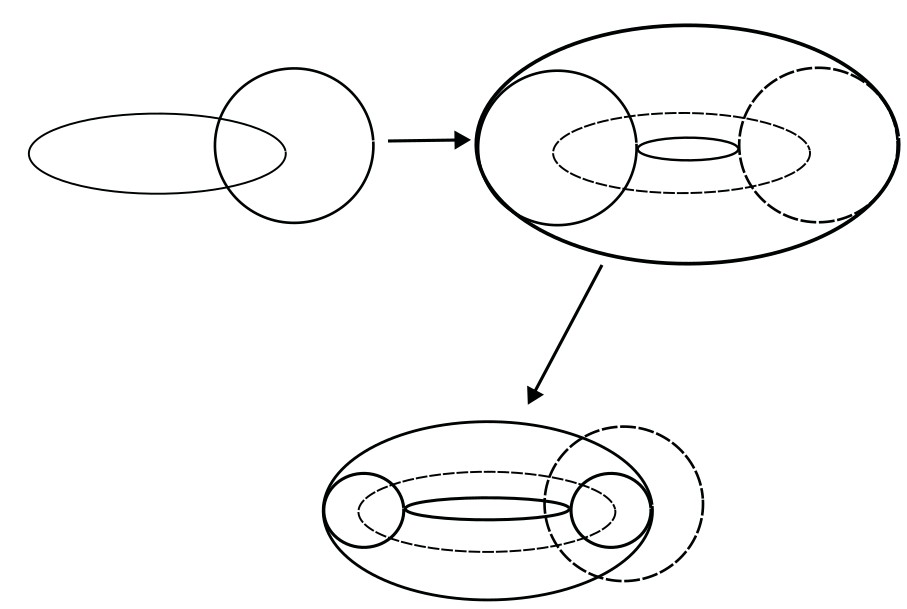
\includegraphics[width = 0.55\textwidth]{../Graphics/1999JII1.jpg}
		\caption{Problem 1999-J-II-1.}
		\label{fig:1999JII1}
	\end{figure}
	
	\begin{prb}{1998-A-I-4}
		Let $A$ denote the subset of 3-space $\mathbb{R}^{3}$ consisting of the union of the $z$-axis, the unit circle centered at the origin in the $xy$-plane, and the point $(3,3,0)$. Set $B = \mathbb{R}^{3}\setminus A$. Show that $\pi_1(B)$ has a subgroup which is isomorphic to $\mathbb{Z}$.
	\end{prb}
	Consider the contruction in Figure \ref{fig:1998AI4}. 
	\begin{figure}[h!]
		\centering
		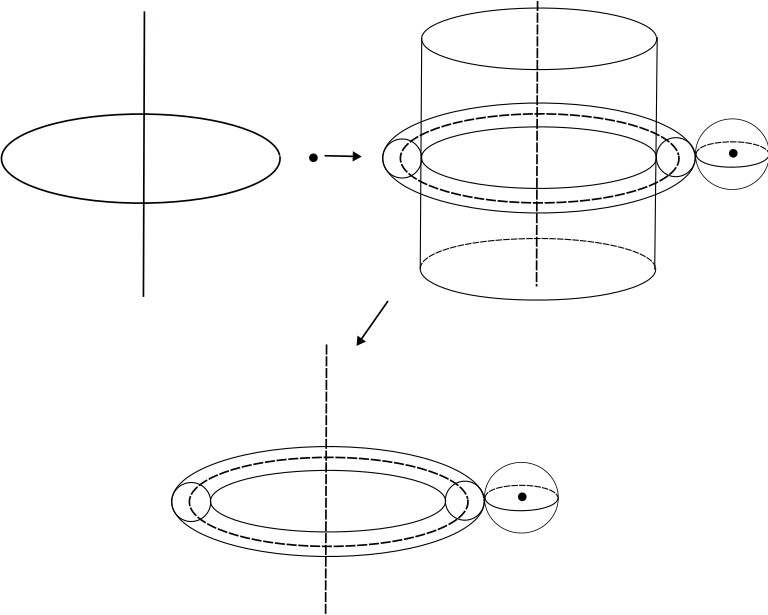
\includegraphics[width = 0.73\textwidth]{../Graphics/1998AI4.jpg}
		\caption{Problem 1998-A-I-4.}
		\label{fig:1998AI4}
	\end{figure}
	
	Thus we see that the space $B$ is homotopy equivalent to the wedge sum $T^{2} \vee S^2$. Therefore, $\pi_{1}(B) \cong \pi_{1}(T^{2}) \ast \pi_{1}(S^{2}) \cong \pi_{1}(T^{2}) \cong \mathbb{Z}^{2}$. Then one has that the subgroup generated by the element $(1,0) \in \mathbb{Z}^{2}$ is precisely the subgroup $\mathbb{Z} \times \{0\}$. Let $\varphi: \mathbb{Z} \times \{0\} \to \mathbb{Z}$ be the standard projection map. Then it is straightforward to show that $\varphi$ is an isomorphism, which concludes the proof. 
	
	\begin{prb}{1997-J-I-2}
		Let $C \subset \mathbb{R}^{3}$ be the unit circle in the $xy$-plane, and let $L \subset \mathbb{R}^{3}$ be the $z$-axis. Let $Y = \mathbb{R}^{3} \setminus (C \cup L)$ be the complement of these two curves. Compute the fundamental group of $Y$. 
	\end{prb}
	Let $Y$ be the space described above. We will demonstrate an explicit construction to show that $Y$ is homotopy equivalent to the 2-torus, $T^{2}$, in Figure \ref{fig:1997JI2}.
	 
	\begin{figure}[h!]
		\centering 
		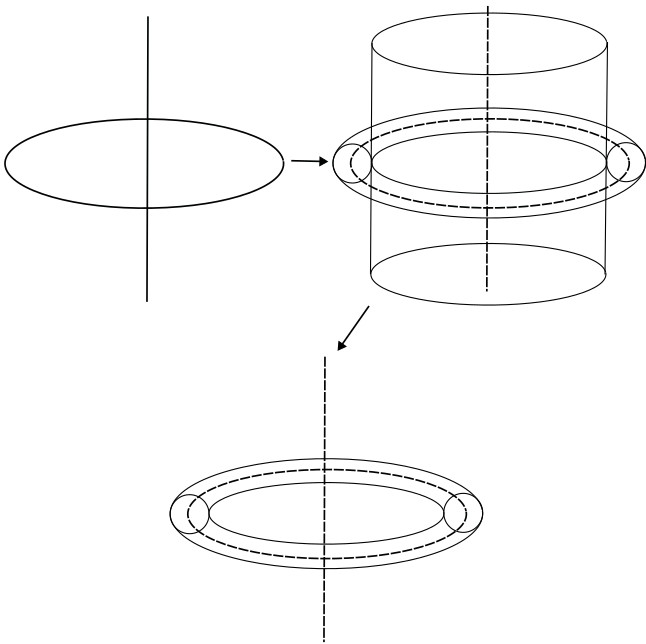
\includegraphics[width = 0.73\textwidth]{../Graphics/1997JI2.jpg}
		\caption{Problem 1997-J-I-2.}
		\label{fig:1997JI2}
	\end{figure}	
	Since $\pi_{1}(T^{2}) \cong \mathbb{Z}^{2}$, we conclude that $\pi_{1}(Y) \cong \mathbb{Z}^{2}$. 
	\begin{prb}{R-DGT-1}
		Compute the fundamental group of the 2-torus $T$ using the Seifert-van Kampen Theorem. 
	\end{prb} 
	Let $T$ denote the 2-torus; we will think of $T$ as a square with identified sides $a$ and $b$. Let $p$ be a point at the center of the square, $V$ a small open neighborhood of $p$ in $T$, and $U = T \setminus \{p\}$. Then $V$ is simply connected, $U \cap V$ is homotopy equivalent to the circle $S^1$, and $U$ deformation retracts onto the wire frame. By the Seifert-van Kampen Theorem, $\pi_{1}(T, x_0) \cong \pi_1(U,x_0) \ast \pi_1(V,x_0)/N$, where $N$ is the normal closure of the subgroup $\braket{i_1^\ast(g)i_2^\ast(g)^{-1}: g\in \pi_1(U \cap V,x_0)}$, $i_1, i_2$ are the inclusion maps of $U \cap V$ into $U$ and $V$, respectively, and $i_1^\ast, i_2^\ast$ are the respective induced maps on fundamental groups. Since $V$ is contractible, $\pi_1(V,x_0) \cong 1$. On the other hand, $\pi_1(U \cap V,x_0) \cong \pi_1(S^1,x_0) \cong \mathbb{Z}$. So let $[\gamma]$ be a generator of the former fundamental group. Since $U$ deformation retracts onto the wire frame, it is homotopy equivalent to the wedge of 2 circles, which has as its fundamental group the free group $\braket{[a],[b]}$ on two generators. Next, it follows that $i_1^\ast([\gamma]) = [\alpha\beta\alpha^{-1}\beta^{-1}] = [\alpha][\beta][\alpha^{-1}][\beta^{-1}]$. Thus one has by the Seifert-van Kampen Theorem that 
	\begin{equation*}
		\pi_1(X,x_0) \cong \braket{[\alpha],[beta] \mid [\alpha][\beta][\alpha]^{-1}[\beta]^{-1} = 1} \cong \mathbb{Z}^{2}. 
	\end{equation*}
	
	
	\begin{prb}{R-DGT-2}
		Compute the fundamental group of $S^1 \vee S^1$ using the Seifert-van Kampen Theorem. 
	\end{prb}
	Let $X$ denote the wedge space $S^1 \vee S^1$. Consider the following depiction of $X$: 
	\begin{figure}[h!]
		\centering 
		\begin{tikzpicture}[scale=0.5]
			% Coordinates
			\coordinate (A) at (0.00, 8.00);
			\coordinate (B) at (0.00, 8.00);
			\coordinate (C) at (4.00, 8.00);
			\coordinate (D) at (4.00, 8.00);
			\coordinate (E) at (-1.40, 9.52);
			\coordinate (F) at (5.50, 9.50);
			
			% Drawing
			\draw[blue, thick] (A) circle (2.00);
			\draw[red, thick] (C) circle (2.00);
			\draw[blue, very thick, dashed] (4.00, 10.00) arc (90.0:-90.0:2.00);
			\draw[red, ultra thick, dashed] (2.00, 8.00) arc (0.0:90.0:2.00);
			\draw[red, ultra thick, dashed] (0.00, 6.00) arc (-90.0:0.0:2.00);
			\node[above, text=blue, font=\LARGE] at (E) {$U$};
			\node[above, text=red, font=\LARGE] at (F) {$V$};
		\end{tikzpicture}
	\end{figure}
	Then we see that $U \cap V$ is homotopy equivalent to a point, and hence is simply connected, and $U, V$ are homotopy equivalent to the circle $S^1$ so that $\pi_1(U,x_0), \pi_1(V,x_0) \cong \mathbb{Z}$. Therefore, since $U \cap V$ is simply connected, by the Seifert-van Kampen Theorem, one has 
	\begin{equation*}
		\pi_1(X, x_0) \cong \pi_1(U,x_0) \ast \pi_1(V,x_0) \cong \mathbb{Z} \ast \mathbb{Z}. 
	\end{equation*}
	
	\begin{prb}{R-DGT-3}
		Compute the fundamental group of the M\"obius strip. 
	\end{prb}
	Consider the constructions in Figure \ref{fig:RDGT3}.  
	\begin{figure}[h!]
		\centering 
		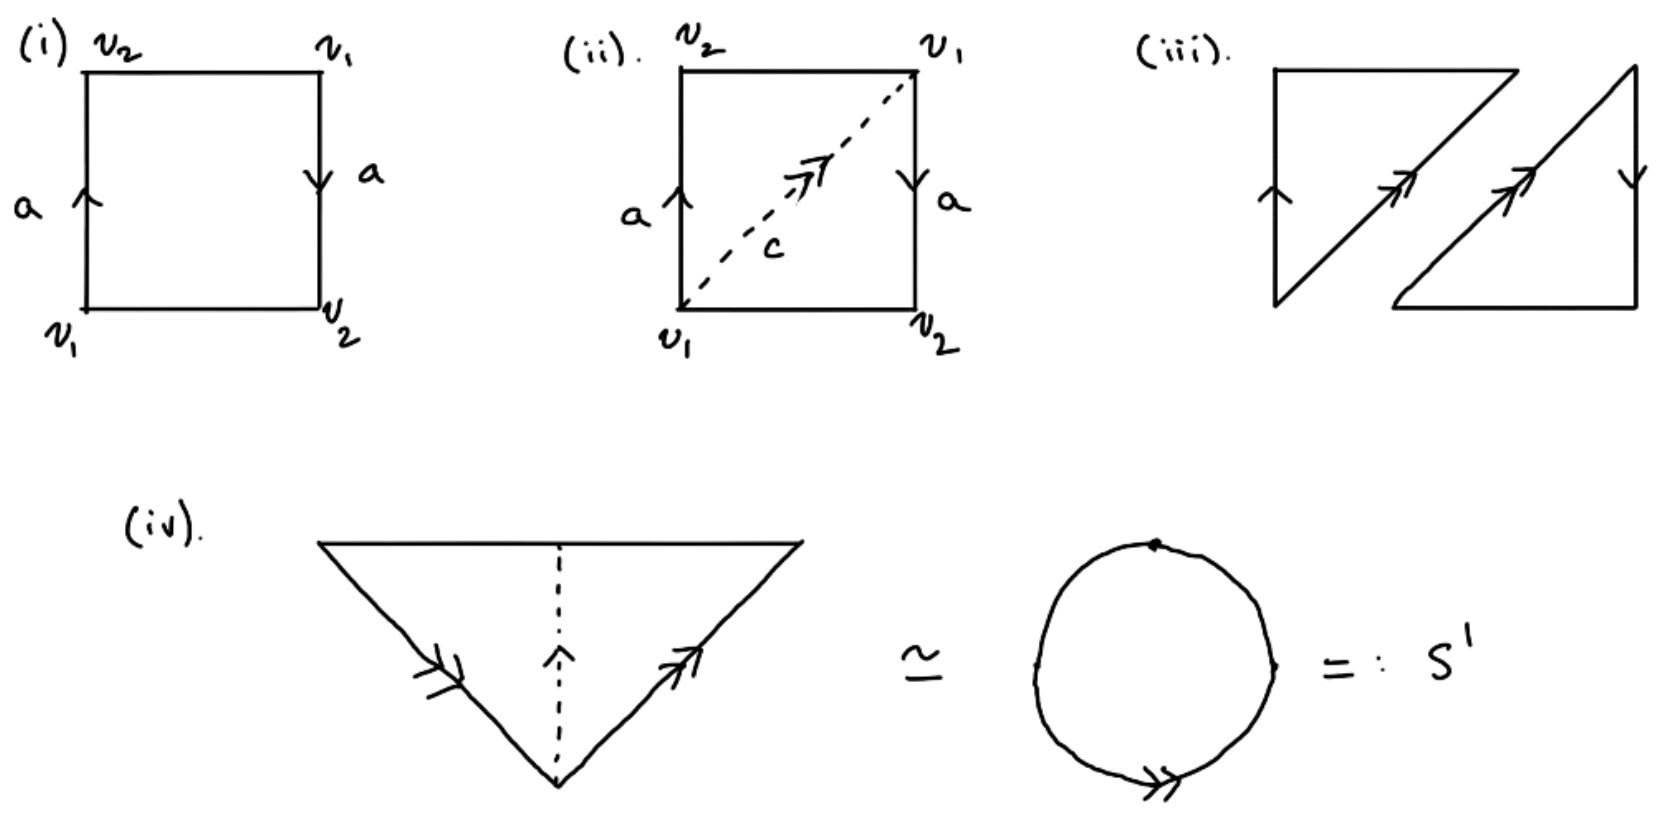
\includegraphics[width = \textwidth]{../Graphics/RDTG3_1.jpg}
		\label{fig:RDGT3}
	\end{figure}
	
	Since the M\"obius strip is homotopy equivalent to $S^1$, and homotopy equivalences, we conclude that $\pi_{1}(M) \cong \pi_1(S^1) \cong \mathbb{Z}$.  
	
	\begin{prb}{R-DGT-4}
		Compute the fundamental group of the 2-torus $T$ using the theory of CW complices. 
	\end{prb}
	Give the 2-torus its standard CW structure (1 0-cell, two 1-cells, and 1 2-cell). The fundamental group of the 1-skeleton (the wire frame) is the free group on two generators $\braket{a,b}$. When we attach the 2-cell along its boundary, the boundary path of the 2-cell traces the product of these edges, defining the attaching map $\partial e^2 = aba^{-1}b^{-1}$. Thus since adding a 2-cell introduces a single relation to the fundamental group of the 1-skeleton, one has that the fundamental group of the torus is 
	\begin{equation*}
		\pi_1(T) \cong \braket{a,b \mid aba^{-1}b^{-1} = 1} \cong \mathbb{Z} \times \mathbb{Z}, 
	\end{equation*}
	exactly as we found above. 
	
	\begin{prb}{H-1.2-4}
		Let $X \subset \mathbb{R}^{3}$ be the union of $n$ lines through the origin. Compute $\pi_{1}(\mathbb{R}^{3} \setminus X)$. 
	\end{prb}
	Let $X$ denote the union of $n$ distinct lines in $\mathbb{R}^{3}$ through the origin. Then $\mathbb{R}^{3}\setminus X$ is homotopy equivalent to the space $S^{2}\setminus \{q_{1}, q_{2}, \ldots, q_{2n}\}$, where the $q_{i}$ are the $2n$ intersection points of the $n$ lines with the circle $S^{n}$. But $S^{2}\setminus \{q_{1}\}$ is homotopy equivalent to $\mathbb{R}^{2}$. Thus one has that $\mathbb{R}^{3}\setminus X$ is homotopy equivalent to $\mathbb{R}^{2}\setminus \{q_{2}, \ldots, q_{2n}\}$, which itself is homotopy equivalent to the bouquet of $2n - 1$ circles. Therefore, using the Seifert-van Kampen theorem, one concludes that $\pi_{1}(\mathbb{R}^{3}\setminus X) \cong F_{2n - 1}$, the free group on $2n - 1$ generators. 
	
	\begin{prb}{H-1.2-7}
		Let $X$ be the quotient space of $S^2$ obtained by identifying the north and south poles to a single point. Put a cell complex structure on $X$ and use this to compute $\pi_{1}(X)$. 
	\end{prb}
	Let $X$ be the quotient space of $S^2$ obtained by identifying the north and south poles to a single point. We first give $S^2$ the CW structure consisting of two 0-cells $N$ and $S$ (corresponding to the north and south poles, respectively), two 1-cells $a$ and $b$ (which map $N \mapsto S$ and $S \mapsto N$, respectively), and two 2-cells $e^{2}_{W}$ and $e^{2}_{E}$ (corresponding to the eastern and western hemispheres, respectively); $\partial e^{2}_{W}$ is attached along the boundary word $ab$, while $\partial e^{2}_{E}$ is attached along the boundary word $b^{-1}a^{-1}$. In $X$, we identify the two poles $N$ and $S$, so that our CW structure reduces to a single 0-cell $N$, the two loops $a$ and $b$ (which are now both based at $N$), and the two 2-cells $e^{2}_{W}$ and $e^{2}_{E}$. Thus by the van Kampen Theorem, one obtains, 
	\begin{equation*}
		\pi_{1}(X) \cong \braket{a, b \mid ab = 1, b^{-1}a^{-1} =1}. 
	\end{equation*}
	The relations give $b = a^{-1}$ so that the loop $b$ is redundant. Thus, $\pi_{1}(X) \cong \braket{a} \cong \mathbb{Z}$. 
	
	\begin{prb}{H-1.2-8}
		Compute the fundamental group of the space obtained from two tori $S^{1} \times S^{1}$ by identifying a circle $S^{1} \times \{x_0\}$ in one torus with the corresponding circle $S^{1} \times \{x_0\}$ in the other torus. 
	\end{prb}
	
	Let $X$ denote the space obtained by identifying the equator circle in one torus with the equator circle of another torus. First, we will compute the fundamental group of $X$ using CW structures. Assign the first torus $T_{1}$ the standard CW structure comprised of one 0-cell $v_{0}$, two 1-cells $e^{1}_{C_{1}}, e^{1}_{R_{1}}$ (where $e^{1}_{C_{1}}$ denotes the equator circle), and one 2-cell $e^{2}_{T_{1}}$; $\partial e^{2}_{T_{1}}$ is attached along the boundary word $e^{1}_{R_{1}}e^{1}_{C_{1}}(e^{1}_{R_{1}})^{-1}(e^{1}_{C_{1}})^{-1}$. For the second torus, we also assign the standard CW structure for the 2-torus: give this structure one 0-cell $w_{0}$, two 1-cells $e^{1}_{C_{2}}, e^{1}_{R_{2}}$ (where $e^{1}_{C_{2}}$ denotes the equator circle), and one 2-cell $e^{2}_{T_{2}}$; $\partial e^{2}_{T_{2}}$ is attached along the boundary word $e_{C_{2}}^{1}e_{R_{2}}^{1}(e_{C_{2}}^{1})^{-1}(e_{R_{2}}^{1})^{-1}$. By gluing the equators of the 2-torus, we identify $e^{1}_{C_{2}} \sim e^{1}_{C_{1}}$ and $v_{0} \sim w_{0}$. Thus, by the van Kampen Theorem, one has that 
	\begin{multline*}
		\pi_{1}(X) \cong \braket{e^{1}_{C_{1}}, e^{1}_{C_{2}}, e^{1}_{R_{1}}, e^{1}_{R_{2}} \mid [e^{1}_{C_{1}}, e^{1}_{R_{1}}] = 1, [e^{1}_{C_{2}}, e^{1}_{R_{2}}] = 1, e^{1}_{C_{1}} = e^{1}_{C_{2}}} \\ = \braket{e^{1}_{C_{1}}, e^{1}_{R_{1}}, e^{1}_{R_{2}} \mid [e^{1}_{C_{1}}, e^{1}_{R_{1}}] = [e^{1}_{C_{1}}, e^{1}_{R_{2}}] = 1}. 
	\end{multline*}
	Alternately, we can use the Seifert-van Kampen Theorem. Let $U$ be the open subset of $X$ consisting of one 2-torus and a small open band around the equator of the second torus, and let $V$ be the open subset consisting of the other 2-torus and a small open band around the equator of the first torus. Then $U \cap V$ deformation retracts onto $S^{1}$ so that $\pi_{1}(U \cap V) \cong \pi_{1}(S^{1}) \cong \mathbb{Z}$. On the other hand, $U$ and $V$ each deformation retract onto a copy of the 2-torus so that $\pi_{1}(U), \pi_{1}(V) \cong \pi_{1}(T^{2}) \cong \mathbb{Z}^{2}$. Therefore, by the Seifert-van Kampen theorem, we conclude that 
	\begin{equation*}
		\pi_{1}(X) \cong \pi_{1}(U) \ast_{\pi_{1}(U \cap V)} \pi_{1}(V) \cong \mathbb{Z}^{2} \ast_{\mathbb{Z}} \mathbb{Z}^{2}, 
	\end{equation*}
	where the amalgamation identifies the cyclic generator of $\mathbb{Z}$ with each of the equatorial generators in each torus. 
	\begin{prb}{H-1.3-9}
		Show that if a path-connected, locally path connected space $X$ has $\pi_{1}(X)$ finite, then every map $X \to S^{1}$ is nullhomotopic. [Use the covering space $\mathbb{R} \to S^{1}$.]
	\end{prb}
	Let $X$ be a path-connected, locally path connected space with finite fundamental group $\pi_{1}(X)$, and let $f: X \to S^{1}$ be a fixed map. Consider the induced map $f_{\ast}: \pi_{1}(X) \to \pi_{1}(S^{1}) \cong \mathbb{Z}$. Since $\mathbb{Z}$ is an infinite group, it follows that $f_{\ast}$ has to be the trivial homomorphism: for any $[\gamma]\in \pi_{1}(X)$, one has that $|f_{\ast}([\gamma])| \mid |\gamma|$; every nonzero element in $\mathbb{Z}$ has infinite order, while $|\gamma| < \infty$, so that $f_{\ast}([\gamma]) = 0$. Thus since $f_{\ast}(\pi_{1}(X, x_{0})) \leq p_{\ast}(\pi_{1}(\mathbb{R}, p^{-1}(x_{0})))$, there exists a lift $\ti{f}: X \to \mathbb{R}$ such that $f = p \circ \ti{f}$. Since $\mathbb{R}$ is contractible, $\ti{f}$ must be nullhomotopic. Projecting down the homotopy via the covering map $p$, it follows that $f$ must be nullhomotopic as well. 
	
	\begin{prb}{H-1.3-10}
		Find all the connected 2-sheeted and 3-sheeted covering spaces of $S^{1} \vee S^{1}$, up to isomorphism of covering spaces without basepoints. 
	\end{prb}
	Let $X$ denote the space $S^{1} \vee S^{1}$, where $\pi_{1}(X) \cong \pi_{1}(S^{1}) \ast \pi_{1}(S^{1}) \cong \mathbb{Z} \ast \mathbb{Z}$. By the Galois correspondence for covering spaces, the isomorphism classes of 2-sheeted and 3-sheeted covering spaces of $S^{1} \vee S^{1}$ correspond to the conjugacy classes of index-2 and index-3 subgroups, respectively, of $\mathbb{Z}\ast \mathbb{Z}$. We consider each case separately. \vspace{-0.25cm}
	\begin{enumerate}[itemsep =-2pt, label = (\roman{*})]
		\item (2-Sheeted Spaces) The conjugacy classes of index-2 subgroups of $\mathbb{Z} \ast \mathbb{Z}$ are in one-to-one correspondence with surjective group homomorphisms $\varphi: \mathbb{Z} \ast \mathbb{Z} \cong \braket{a, b} \to \mathbb{Z}_{2}$. To obtain a surjective group homomorphism, at least one of the generators must map to the element $1 \in \mathbb{Z}_{2}$. Thus we obtain three distinct homomorphisms: (1) $a \mapsto 1, b \mapsto 0$, (2) $a \mapsto 0, b \mapsto 1$, and (3) $a \mapsto 1, b \mapsto 1$. Since $\operatorname{Aut}(\mathbb{Z}_{2})$ is trivial, it follows that each homomorphism corresponds to a distinct isomorphism class\footnote{Case 1 ($\phi_1$): $a$ traverses across the two sheets (a double loop), while $b$ lifts to two separate loops (one on each sheet).Case 2 ($\phi_2$): Symmetric to Case 1, with the roles of $a$ and $b$ flipped.Case 3 ($\phi_3$): Both $a$ and $b$ traverse across the two sheets, forming a 2-vertex graph where two $a$-edges and two $b$-edges alternate between the vertices.} Thus, visually the three 2-sheeted covering spaces of $S^{1} \vee S^{1}$ are given in Figure \ref{fig:H1310}. 
		\begin{figure}[h!]
			\centering 
			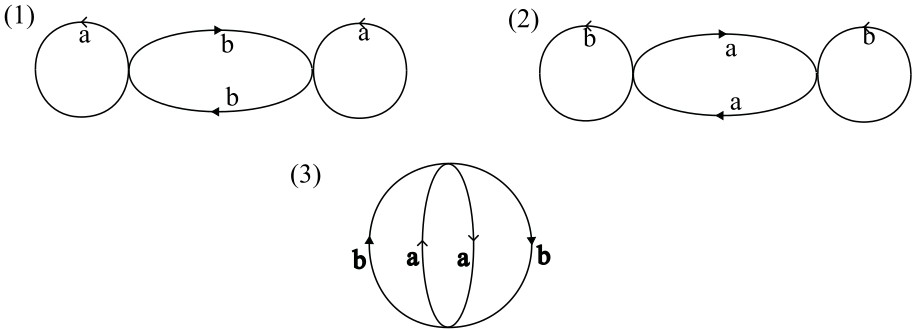
\includegraphics[width = \textwidth]{../Graphics/H1310.jpg}
			\caption{Problem H-1.3-10.}
			\label{fig:H1310}
		\end{figure}
		
		\item (3-Sheeted Spaces) First, we will obtain the regular 3-sheeted covering spaces of $X$, which correspond to surjective homomorphisms $\varphi: \mathbb{Z} \ast \mathbb{Z} \to \mathbb{Z}_{3}$. Here, we have more options. However, since $\operatorname{Aut}(\mathbb{Z}_{3}) \cong \mathbb{Z}_{2}$, some distinct surjective homomorphisms may produce isomorphic covering spaces. Any homomorphism from $\mathbb{Z} \ast \mathbb{Z} \cong \braket{a,b} \to \mathbb{Z}_{3}$ is surjective as long as it is nonzero. Thus we find there are exactly 4 regular 3-sheeted covering spaces: (1) $b$ traverses three sheets, while $a$ lifts to three separate loops on each sheet, (2) symmetric to case (1) with $a$ and $b$ flipped, (3) both $a$ and $b$ traverse three sheets, (4) both $a$ and $b$ traverse three sheets, but in opposite directions. Now we will look for non-regular 3-sheeted covering spaces, which correspond to transitive homomorphisms $\varphi: \mathbb{Z} \ast \mathbb{Z} \to S_{3}$, up to conjugation by elements in $S_{3}$. Since there are a total of 13 subgroups of $\mathbb{Z}\ast \mathbb{Z}$ of index 3, and 4 are normal, 9 must be nonnormal subgroups, corresponding to the non-regular 3-sheeted covering spaces of $X$. Since $3$ is prime, the normalizer of any non-normal index-3 subgroup $H$ is $H$ itself. Thus, each non-normal subgroup has exactly $3$ conjugates in $\mathbb{Z} \ast \mathbb{Z}$. This means that there exist precisely 3 conjugacy classes of nonnormal index-3 subgroups, and thus exactly 3 isomorphism classes of non-regular 3-sheeted covering spaces of $X$. Altogether, there are 7 3-sheeted covering spaces of $X$ (of which $4$ are normal.)
	\end{enumerate}
	
	\newpage 
	\subsection{Vector Fields}
	\begin{prb}{2020-J-I-4}
		Let $\theta$ be a closed smooth 1-form on a compact $C^{\infty}$ manifold $M$ with empty boundary, and let $v$ be a smooth vector field on $M$. Prove that the Lie derivative $\mathcal{L}_{v}\theta$ vanishes at some point of $M$. 
	\end{prb}
	Let $\theta$ be a closed smooth 1-form on a smooth manifold $M$ without boundary, and let $V$ be a smooth vector field on $M$. By Cartan's formula, 
	\begin{equation*}
		\mathcal{L}_{V}\theta = V \contract d\theta + d(V \contract \theta) = d(V \contract \theta), 
	\end{equation*}
	where the first term is identically zero since $\theta$ is closed. Since $\theta$ is a smooth 1-form, $V \contract \theta$ is a smooth 0-form on $M$; i.e., $V \contract \theta$ is a smooth function from $M$ to $\mathbb{R}$. Then by the extreme value theorem, $V \contract \theta$ must have an extrema at some point $p \in M$, which means that $d(V \contract \theta) = 0$ at $p$. But this means that $\mathcal{L}_{V}\theta$ vanishes at $p \in M$. Thus, the proof concludes. 
	
	\begin{prb}{2017-J-II-1}
		Let $f: M \to \mathbb{R}$ be a smooth function on a manifold $M$. In any arbitrary smooth local coordinate chart $x: U \to \mathbb{R}^{n}$ of $M$, define 
		\begin{equation*}
			\mathcal{D}f \coloneqq \sum_{i = 1}^{n}\frac{\partial f}{\partial x^{i}}\frac{\partial}{\partial x^{i}}. 
		\end{equation*}
		Does $\mathcal{D}f$ give a well-defined vector field on $M$? 
	\end{prb}
	Let $f: M \to \mathbb{R}$ be a smooth function on a manifold $M$, and define $\mathcal{D}f$ as given above. We claim that $\mathcal{D}f$ does \textit{not} give a well-defined vector field on $M$. Let $(U, (x^{i})), (V, (\ti{x}^{j}))$ be overlapping coordinate charts. At any $p \in U \cap V$, we have 
	\begin{align*}
		\begin{split}
			\mathcal{D}f &= \frac{\partial f}{\partial x^{i}}\frac{\partial}{\partial x^{i}} \\
			&= \left(\frac{\partial f}{\partial \ti{x}^{j}}\frac{\partial \ti{x}^{j}}{\partial x^{i}}\right)\cdot \left(\frac{\partial}{\partial \ti{x}^{j}}\frac{\partial \ti{x}^{j}}{\partial x^{i}}\right) \\
			&= \left(\frac{\partial \ti{x}^{j}}{\partial x^{i}}\right)^{2}\cdot \left(\frac{\partial f}{\partial \ti{x}^{j}}\frac{\partial}{\partial \ti{x}^{j}}\right). 
		\end{split}
	\end{align*}
	I.e., $\mathcal{D}f$ does not follow the correct transformation law for tangent vector fields, so that the proof concludes.  
	
	\begin{prb}{AZ-2011-M-1}
		Suppose $M$ is a smooth manifold, $X, Y \in \Gamma(M; TM)$ are smooth vector fields on $M$, and $g \in C^{\infty}(M)$ is a smooth function on $M$. Show \textit{directly from the definition} that 
		\begin{equation*}
			[gX, Y] = g[X, Y] - Y(g)X. 
		\end{equation*}
		(You can assume that $[\cdot, \cdot]$ is whatever object it is supposed to be, but do state what you are taking it to be.)
	\end{prb}
	Let $M$ be a smooth manifold, and $X, Y$ be smooth vector fields on $M$. Further assume $g \in C^{\infty}(M)$ is a smooth function on $M$. We note that $[X, Y]$ denotes the Lie bracket of $X$ and $Y$, and is a smooth vector field on $M$. Let $\varphi \in C^{\infty}(M)$ be an arbitrary test function. Then one has that
	\begin{align*}
		\begin{split}
			[gX,Y](\varphi) &= (gX \circ Y)(\varphi) - (Y \circ gX)(\varphi) \\
			&= (gX \circ Y)(\varphi) - Y(g) \cdot X(\varphi) - g (Y \circ X)(\varphi) \\
			&= \left(g(X \circ Y)(\varphi) - g(Y \circ X)(\varphi)\right) - Y(g) \cdot X(\varphi) \\
			&= g[X,Y](\varphi) - Y(g) \cdot X(\varphi), 
		\end{split}
	\end{align*}
	where in the second line, we used the fact that $Y$ is a derivation and thus satisfies the product rule; in the fourth line, we used the definition of the Lie bracket. Since $\varphi \in C^{\infty}(M)$ was arbitrary, we conclude that $[gX,Y] = g[X,Y] - Y(g)X$. 

	
	\subsection{Covering Spaces}
	
	\begin{prb}{2026-J-II-1}
		For every even integer $g$ and $g$-holed torus $\Sigma_g$, prove that there is no continuous, fixed-point free orientation-preserving involution of $\Sigma_g$. 
	\end{prb}
	Let $g$ be an even integer, $\Sigma_g$ be a $g$-holed torus, and assume to the contrary that there exists a fixed-point free orientation-preserving involution $\tau: \Sigma_g \to \Sigma_g$. Since $\tau^2 = \operatorname{id}$, $\tau$ defines a free action of $\mathbb{Z}/2\mathbb{Z}$ on $\Sigma_g$. Therefore, the quotient space $X = \Sigma_g/\braket{\tau}$ is a closed surface, and the quotent mapping $\Sigma_g \to X$ is a 2-sheeted covering map. Since $\tau$ is orientation-preserving, $X$ is orientable. Therefore, $X \cong \Sigma_h$ for some $h \geq 0$. The genus of $\Sigma_h$ is $2 -2h$. And since $\Sigma_g$ is a 2-sheeted covering space of $\Sigma_h$, we must have 
	\begin{equation*}
		2 - 2g = 2(2 - 2h) = 4 - 4h \implies 2g = 4h -2 \implies g = 2h -1, 
	\end{equation*}
	which contradicts our hypothesis that $g$ is even. Thus by contradiction, there cannot be a fixed-point free orientation-preserving involution. 
	
	\begin{prb}{2025-J-II-2}
		Determine all path connected covering spaces having base space $\mathbb{RP}^2 \times \mathbb{RP}^2$, up to equivalence, where two covering spaces $\pi_1: X \to \mathbb{RP}^2 \times \mathbb{RP}^2$ and $\pi_2: Y \to \mathbb{RP}^2 \times \mathbb{RP}^2$ are defined to be equivalent if there is a homeomorphism $\phi: X \to Y$ such that $\pi_1 = \pi_2 \circ \phi$. 
	\end{prb}
	Let $X$ denote the base space $\mathbb{RP}^2 \times \mathbb{RP}^2$. By the Galois correspondence of covering spaces, there exists a one-to-one correspondence between isomorphism classes of connected covering spaces and conjugacy classes of subgroups of $\pi_1(X)$. Since $\pi_1(\mathbb{RP}^2) \cong \mathbb{Z}/2\mathbb{Z}$, $\pi_1(x) \cong \mathbb{Z}/2\mathbb{Z} \times \mathbb{Z}/2\mathbb{Z}$. We note the following subgroups of $\pi_1(X)$: 
	\begin{enumerate}[itemsep =-2pt,label = (\arabic{*})]
		\item The whole group, $\mathbb{Z}/2\mathbb{Z} \times \mathbb{Z}/2\mathbb{Z} \cong \braket{(0,1),(1,0)}$ 
		\item $\{(0,0), (1,1)\}$
		\item $\{(0,0), (0,1)\} \cong \{0\} \times \mathbb{Z}/2\mathbb{Z}$ 
		\item $\{(0,0), (1,0)\} \cong \mathbb{Z}/2\mathbb{Z} \times \{0\}$. 
		\item The trivial subgroup, $\{(0,0)\}$
	\end{enumerate}
	Since $\pi_1(X)$ is abelian, every subgroup is normal, which means that each of the above subgroups belongs to its own conjugacy class. The trivial subgroup corresponds to the covering space $S^2 \times S^2$, which is path connected since $S^2$ is path connected. The whole group itself corresponds to the covering space $\mathbb{RP}^2 \times \mathbb{RP}^2$, which is path-connected since each $\mathbb{RP}^2$ is a path-connected space. The subgroups $\{(0,0), (0,1)\}, \{(0,0),(1,0)\}$ correspond to the pa..th-connected spaces $S^2 \times \mathbb{RP}^2$ and $\mathbb{RP}^2 \times S^2$. Now we know that every manifold $M$ has an orientable orientation cover (which corresponds with an index 2 subgroup of $\pi_1(M)$). Since neither $\{(0,0), (0,1)\}$ nor $\{(0,0), (1,0)\}$ (which are the only other index 2 subgroups) correspond to orientable covering spaces, it follows that $\{(0,0), (1,1)\}$ must correspond to the orientation cover of $X$. Thus since $X$ is non-orientable (since each factor is nonorientable), the orientation cover of $X$ must necessarily be path-connected. Thus up to isomorphism, $X$ has precisely 5 path-connected covering spaces, 2 of which are orientable. 
	
	\begin{prb}{2024-A-I-3}
		Let $\gamma$ be a closed curve in $\mathbb{C}\setminus \{0\}$ with winding number $1$ around the origin. Show that the curve $\gamma$ contains two points that are negatives of each other in $\mathbb{C}$. 
	\end{prb}
	Suppose to the contrary that $\gamma$ contains no antipodal points. Then the function $f(z) = z^2$ must be injective on $\gamma$ so that $f(\gamma)$ is a Jordan curve.\footnote{A Jordan curve is a simple closed curve that is homeomorphic to the unit circle $S^1$.} Since $0 \notin \gamma$, $0 \notin f(\gamma)$. Moreover, since $f(\gamma)$ is a Jordan curve, its winding number must be $-1$, $0$, or $1$. But since $z^2$ wraps $\gamma$ (which has winding number 1 by the hypothesis) twice, it follows that $f(\gamma)$ must have winding number 2, which is a contradiction. Thus by contradiction, $\gamma$ must contain antipodal points. 
	
	\begin{prb}{2023-J-I-3}
		Show that if $M$ is a closed manifold that has an even dimensional sphere $S^{2n}$ as its universal cover, then its fundamental group is either trivial or $\mathbb{Z}/2\mathbb{Z}$. 
	\end{prb}
	Let $M$ be a closed manifold that has an even dimensional sphere $S^{2n}$ as its universal cover. Let $\Gamma$ be the group of deck transformations\footnote{Note that a \textbf{deck transformation} is a homeomorphism $f: \ti{M} \to \ti{M}$ such that $p \circ f = p$, where $p: \ti{M} \to M$ is the covering map. In particular, deck transformations have the uniqueness property that states that if two such transformations are equal at any point $x \in \ti{M}$, then the two transformations are identical. Moreover, the identity map on $\ti{M}$ is a deck transformation. Thus if the deck transformation $h$ has a fixed point, then it must be the identity map.} on $S^{2n}$ (note that this implies $\pi_1(X) \cong \Gamma$, and every nonidentity element of $\Gamma$ acts freely on $S^{2n}$). Suppose $h: S^{2n} \to S^{2n}$ is fixed-point free. Then since every nontrivial deck transformation must be homotopic to the antipodal map on $S^2n$, and the antipodal map on $S^{2n}$ has degree $(-1)^{2n + 1} = -1$, every nonidentity deck transformation must have degree $-1$. This means that for every $g \in \Gamma$, $\deg{g_1^2} = \deg{g}\cdot \deg{g} = 1$ so that $g^2 = \operatorname{id}$. Thus one possibility is that every $\Gamma$ contains only the trivial element. On the other hand, if one assumes that $\Gamma$ has two nonidentity elements, then since 
	\begin{equation*}
		\operatorname{id} = g_1g_2 \implies g_1 = g_2^{-1}, 
	\end{equation*}
	and inverses are unique, one has that $g_{1}^{-1} = g_{2}^{-1}$ so that $g_1 = g_2$. Thus, $\Gamma$ can contain at most one nontrivial element. This means that either $\Gamma = \{e\}$ or $\Gamma \cong \mathbb{Z}/2\mathbb{Z}$. Since $S^{2n}$ is simply connected for every $n \geq 1$, we conclude that 
	\begin{equation*}
		\pi_{1}(M) \cong \Gamma \cong 
		\begin{cases}
			\{e\} \\
			\mathbb{Z}/2\mathbb{Z}. 
		\end{cases}
	\end{equation*}
	
	\begin{prb}{2022-J-I-2}
		Let $\mathbb{T}^{2} = \mathbb{R}^2/\mathbb{Z}^2$, where $\mathbb{Z}^2 \subset \mathbb{R}^2$ is the standard integer lattice. Is it true that (a) every continuous map $f: S^2 \to \mathbb{T}^2$ is nullhomotopic? (b) every continuous map $g: \mathbb{T}^2 \to S^{2}$?
	\end{prb}
	Let $\mathbb{T}^2 = \mathbb{R}^2/\mathbb{Z}^{2}$ be the $2$-torus. \vspace{-0.25cm}
	\begin{enumerate}[itemsep=-2pt,label = (\alph{*})]
		\item Let $f: S^{2} \to \mathbb{T}^{2}$ be a continuous map. First, we note that $\pi_{1}(S^2) = 1$ since $S^2$ is simply connected. On the other hand, since $\mathbb{T}^{2} \cong S^1 \times S^1$, $\pi_1(T^2, x_0) \cong \mathbb{Z}^2$. Therefore, the induced map $f_\ast(\pi_1(S^2,x_0)) = \{1\}$. Since $\mathbb{T}^2$ is locally path connected and semilocally simply connected, it has a universal covering space; it's universal covering space is $\mathbb{R}^2$. Let $p: \mathbb{R}^2 \to \mathbb{T}^2$ denote the covering map. Since $f_{\ast}(\pi_1(S^2,x_0)) = \{1\} \subset p_\ast(\pi_1(\mathbb{R}^2, x_0))$, $f$ lifts to a map $\ti{f}: S^2 \to \mathbb{R}^2$. But since $\mathbb{R}^{2}$ is contractible, $\ti{f}$ must be nullhomotopic. Thus projecting down, it follows that $f$ must be nullhomotopic. I.e., every continuous map $f: S^2 \to \mathbb{T}^2$ is nullhomotopic. 
		\item \complete 
	\end{enumerate}
	
	\begin{prb}{2021-A-I-6}
		What connected spaces can be finitely-sheeted covering spaces of a sphere with three handles? \label{prb:2021-A-I-6}
	\end{prb}
	Let $\Sigma_{3}$ denote the compact connected orientable surface of genus 3, which is diffeomorphic to the sphere with three handles. Further, we will show that for every positive integer $k \geq 1$, $\Sigma_{3}$ has a $k$-sheeted covering space. Consider the map $\phi: \pi_{1}(\Sigma_{3}) \to \mathbb{Z}/k\mathbb{Z}$ defined by 
	\begin{equation*}
		\phi(a_{1}) = 1 \qquad \text{and} \qquad \phi(a_{2}), \phi(a_{3}), \phi(b_{1}), \ldots, \phi(b_{3}) = 0, 
	\end{equation*}
	where 
	\begin{equation*}
		\pi_{1}(\Sigma_{3}) = \braket{a_{1}, b_{1}, \ldots, a_{3}, b_{3}: [a_{1},b_{1}][a_{2},b_{2}][a_{3},b_{3}] = 1}. 
	\end{equation*}
	Since $1$ is a generator of the additive group $\mathbb{Z}/k\mathbb{Z}$, it follows that $\phi$ is surjective. It is then straightforward to check that $\phi$ is a well-defined group homomorphism. Let $H$ denote the kernel of $\phi$, which is a normal subgroup of $\pi_{1}(\Sigma_{3})$. Thus by the First Isomorphism Theorem, one has that $\pi_{1}(\Sigma_{3})/H \cong \mathbb{Z}/k\mathbb{Z}$. Since $|\mathbb{Z}/k\mathbb{Z}| = k$, $H$ is a subgroup of $\pi_{1}(\Sigma_{3})$ of index $k$. Therefore, by the Galois correspondence for covering spaces, $\Sigma_{3}$ has a $k$-sheeted covering space. Now let $\rho: \ti{M} \to \Sigma_{3}$ be a $k$-sheeted covering space. Then we must have 
	\begin{equation*}
		\chi(\ti{M}) = k \cdot \chi(\Sigma_{3}) \iff 2 - 2g = -4k \iff g = 2k + 1. 
	\end{equation*}
	I.e., $\ti{M}$ must be a surface of genus $2k + 1$. Therefore, we conclude that the only connected finite $k$-sheeted covering spaces of a sphere with three handles are the surfaces $\Sigma_{2k + 1}$, $k \geq 1$. 
	
	\begin{prb}{2020-J-II-6}
		Let $\Phi: S^2 \to S^2$ be a smooth self-map of the 2-sphere which has non-zero degree. Prove that there exists an $\vec{x} \in S^2$ such that $\Phi(-\vec{x}) =-\Phi(\vec{x})$. 
	\end{prb}
	Let $\Phi: S^2 \to S^2$ be a smooth self-map of the 2-sphere which has non-zero degree. Assume to the contrary that there exists no $\vec{x} \in S^2$ such that $\Phi(-\vec{x}) = -\Phi(\vec{x})$. Consider the map $H: S^2 \times [0,1] \to S^2$ defined as follows: 
	\begin{equation*}
		H(\vec{x}, t) = \frac{(1 - t)\Phi(-\vec{x}) + t\Phi(\vec{x})}{\norm{(1 - t)\Phi(-\vec{x}) + t\Phi(\vec{x})}}
	\end{equation*}
	Hence, $H$ is a smooth homotopy between $\Phi$ and $\Phi \circ \alpha$, where $\alpha: S^2 \to S^2$ is the antipodal map. Since the degree of a smooth map is homotopy invariant, one has 
	\begin{equation*}
		\deg(\Phi) = \deg{\Phi \circ \alpha} = (\deg{\Phi})(\deg{\alpha}) = -\deg{\Phi}. 
	\end{equation*}
	But this is only possible iff $\deg{\Phi} = 0$, which is a contradiction. Thus, there has to be a $\vec{x} \in S^{2}$ such that $\Phi(-\vec{x}) = -\Phi(\vec{x})$. 
	
	
	\begin{prb}{2019-J-II-1}
		Let $p: E \to B$ be a covering map such that $B$ is connected and compact, and $p^{-1}(b)$ is finite for some $b \in B$. Show that $E$ is compact. 
	\end{prb}
	Let $p: E \to B$ be a covering map such that $B$ is connected and compact, and $p^{-1}(b_{0})$ is finite for some $b_{0} \in B$; i.e., assume that $1 \leq |p^{-1}(b_{0})| \eqqcolon k < \infty$. We will start by showing that for any $b \in B$, $|p^{-1}(b)| = k$. Define the set $W = \{b \in B: |p^{-1}(b)| = k\}$; $W$ is nonempty since it contains the point $b_{0}$. Now let $b' \in W$, and let $U'$ be an evenly covered neighborhood of $b'$. Then it follows that 
	\begin{equation*}
		p^{-1}(U) = \bigsqcup_{1}^{k}V_{j}, 
	\end{equation*}
	where each $V_j$ is an open subset of $E$ and $p|_{V_{j}} \to U'$ is a homeomorphism. Assume to the contrary that there exists some $b_{0} \in U$ such that $|p^{-1}(b_{0})| \neq k$. This opens up two possibilities: (1) eithe $|p^{-1}(b_{0})| > k$ and at least one of the $V_{j}$ must contain more than one preimage of $b_{0}$ (which is a contradiction since $p|_{V_{j}} \to U$ is injective), or (2) $|p^{-1}(b_{0})| < k$, which means there exists at least one $V_{j}$ with no points $e \in V_{j}$ such that $p(e) = b_{0}$ (whichis a contradiction since $p|_{V_{j}} \to U$ is surjective). Thus, we conclude that $U \subset W$, which implies that $W$ is open. Likewise, we can show that the complement of $W$, $W^{c}$, in $B$ must be open so that $W$ is closed in $B$. Since $B$ is connected, we conclude that $W = B$. 
	
	Now let $\{U_{\alpha}\}$ be an arbitrary open cover of $E$; to show that $E$ is compact, it suffices to show that this open cover has a finite open subcover. Fix an arbitrary $b \in B$, and assume that $p^{-1}(b) = \{e_{1}, \ldots, e_{k}\}$. Then since the $U_{\alpha}$ cover $X$, there exist $U_{\alpha_{1}}, \ldots, U_{\alpha_{k}}$ such that for each $j = 1, \ldots, k$, $e_{j} \in U_{\alpha_{j}}$. Let $p^{-1}(W_{b}) = \bigsqcup_{1}^{k}V_{j}$, where each $V_{j}$ is an open subset of $U$, $e_{j} \in V_{j}$, and $p|_{V_{j}} \to U$ is a homeomorphism. In particular, $p(V_{j} \cap U_{\alpha_{j}})$ is an open neighborhood of $b$ in $B$ for each $j$. So define, 
	\begin{equation*}
		U_{b} = \bigcap_{1}^{k}p(V_{j} \cap U_{\alpha_{j}}),
	\end{equation*}
	which is an open neighborhood of $b$ in $B$. Consider the collection $\{U_{b}\}_{b \in B}$, where for each $b \in B$, $U_{b}$ is constructed as detailed above; this collection is an open cover of $B$. By compactness of $B$, there exists a finite open subcover $\{U_{b_{j}}\}_{j = 1}^{n}$ of $B$. As we detailed above, for each $j$, one has 
	\begin{equation*}
		p^{-1}(U_{b_{j}}) = \bigsqcup_{l = 1}^{k}V_{j,l}, \qquad V_{j,l} \subset U_{\alpha_{l}}^{j}. 
	\end{equation*} 
	Thus, we have a finite subcollection (of $nk$) open subsets $\{U^j_{\alpha_l}\mid j = 1, \ldots, n; l = 1, \ldots, k\}$, and one has 
	\begin{align*}
		\begin{split}
			E &= p^{-1}(B) = p^{-1}\left(\bigcup_{j = 1}^{n}U_{b_{j}}\right) = \bigcup_{j = 1}^{n}p^{-1}(U_{b_{j}}) \\
			&= \bigcup_{j = 1}^{n}\left(\bigsqcup_{l = 1}^{k}V_{j,l}\right) \subset \bigcup_{j = 1}^{n}\bigcup_{l = 1}^{k}U^{j}_{\alpha_{l}}. 
		\end{split}
	\end{align*}
	Thus, since an arbitary open subcover of $E$ admits a finite open subcover, we conclude that $E$ is compact. 
	
	\begin{prb}{2017-J-II-4}
		Let $X = \mathbb{RP}^{2} \vee \mathbb{RP}^{2}$ be the ``wedge'' of two real projective planes, meaning the quotient space obtained from the disjoint union $\mathbb{RP}^{2} \sqcup \mathbb{RP}^{2}$ by identifying a single point $p$ in one copy of $\mathbb{RP}^{2}$ with a single point $\check{p}$ in the other: 
		\begin{center}
			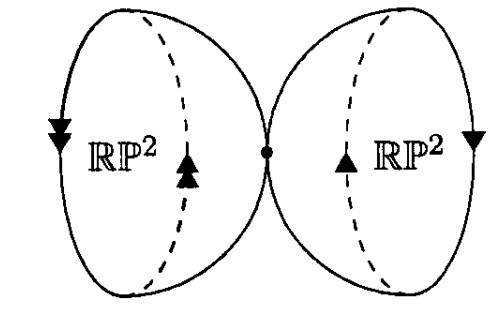
\includegraphics[scale=0.3]{../Graphics/2017JII4}
		\end{center}
		\begin{enumerate}[itemsep =-2pt,label =(\arabic{*})]
			\item What is the fundamental group of $X$? 
			\item Give a concrete description of the universal cover $\ti{X}$ of $X$, accompanied by a drawing of $\ti{X}$. 
		\end{enumerate}
	\end{prb}
	Let $X = \mathbb{RP}^{2} \vee \mathbb{RP}^{2}$ denote the wedge of two real projective planes. \vspace{-0.25cm}
	\begin{enumerate}[itemsep =-2pt,label = (\arabic{*})]
		\item Let $U$ be the open subset obtained by taking the union of the left copy of $\mathbb{RP}^{2}$ with a small neighborhood $\ti{U}$ of $p$ contained in the right copy of $\mathbb{RP}^{2}$. Likewise, let $V$ be the open subset of $X$ obtained by taking the union of the right copy of $\mathbb{RP}^{2}$ with a small neighborhood $\ti{V}$ of $p$ contained in the left copy of $\mathbb{RP}^{2}$. We see that both $U$ and $V$ are path connected (since $\mathbb{RP}^{2}$ is path connected), and deformation retract onto the respective copies of $\mathbb{RP}^{2}$ so that $\pi_{1}(U), \pi_{1}(V) \cong \pi_{1}(\mathbb{RP}^{2})$. Moreover, $U \cap V$ deformation retracts onto the identified points so that $\pi_{1}(U \cap V)$ is the trivial subgroup. Therefore, by the Seifert-van Kampen theorem, since $\pi_{1}(\mathbb{RP}^{2}) \cong \mathbb{Z}/2\mathbb{Z}$, we conclude that 
		\begin{equation*}
			\pi_{1}(X) \cong \pi_{1}(U) \ast_{\pi_{1}(U \cap V)} \pi_{1}(V) \cong \mathbb{Z}/2\mathbb{Z} \ast \mathbb{Z}/2\mathbb{Z}. 
		\end{equation*}
		\item We recall that the universal cover of $\mathbb{RP}^{2}$ is $S^{2}$, which is a 2-sheeted covering space (since the covering map is the quotient map that identifies antipodal points on $S^{2}$ so that each point on $\mathbb{RP}^{2}$ corresponds to two (antipodal) points on $S^{2}$). To construct the universal cover $\ti{X}$, we start with a copy of $S^{2}$. To each lift $\bar{p}$ of $p$, we attach a copy of $S^{2}$ by identifying that $\bar{p}$ to some lift $\bar{\check{p}}$ of $\check{p}$. To each unidentified lift $\bar{\check{p}}$, we attach another copy of $S^{2}$ by identifying that $\bar{\check{p}}$ to some lift of $p$. We repeat this procedure indefinitely. Thus the universal cover $\ti{X}$ resembles an infinite chain of spheres $S^{2}$. 
		\begin{figure}[h!]
			\centering 
			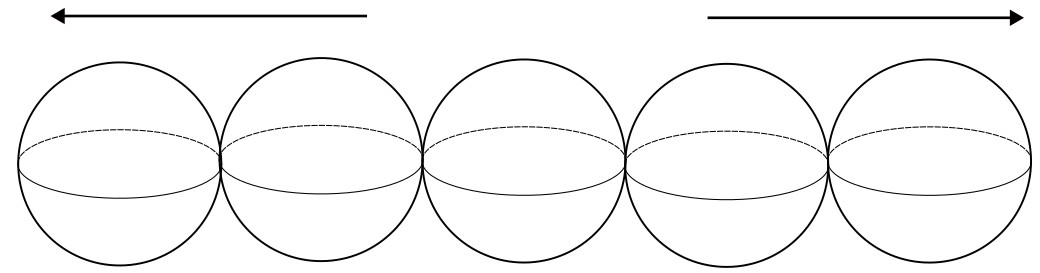
\includegraphics[scale = 0.4]{../Graphics/2017JII4_uc.jpg}
		\end{figure}
	\end{enumerate}
	
	\begin{prb}{2016-A-II-1}
		Let $X$ be the topological space obtained by making a 2-sphere and a 2-torus touch at a single point: 
		\begin{center}
			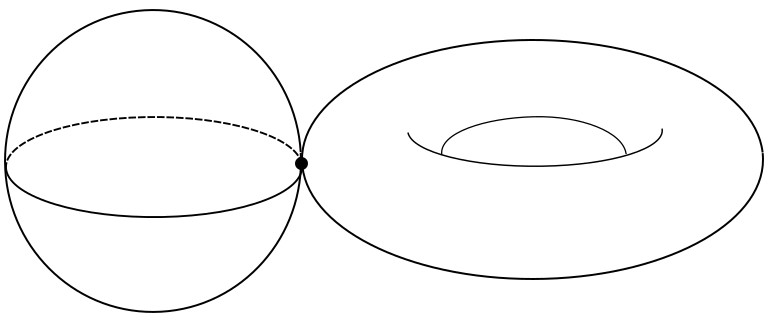
\includegraphics[scale = 0.4]{../Graphics/2016AII1.jpg}
		\end{center}
		Give a concrete description of the universal cover $\ti{X}$ of $X$, accompanied by a drawing of $\ti{X}$. 
	\end{prb}
	Let $X$ be the topological space obtained by identifying a single point on $S^{2}$ with a single point on $T^{2}$; i.e., let $X = S^{2} \vee T^{2}$. Let $p \in S^2$ and $q \in T^2$ be the points of identification. We recall that the universal cover of $S^{2}$ is itself, and the covering map has 1 sheet. On the other hand, the universal cover of $T^{2}$ is $\mathbb{R}^{2}$. We start with the universal cover $\ti{S}^{2}$. To the lift $\bar{p}$ of $p$, we attach a copy of $\mathbb{R}^2$, by identifying $\bar{p}$ to some lift $\bar{q}$ of $q$. Next, for each unidentified lift $\bar{q}$ of $q$, we then attach a copy of $S^{2}$, by identifying that $\bar{q}$ with $\bar{p}$. Visually, the universal cover of $X$ resembles the following: 
	\begin{figure}[h!]
		\centering 
		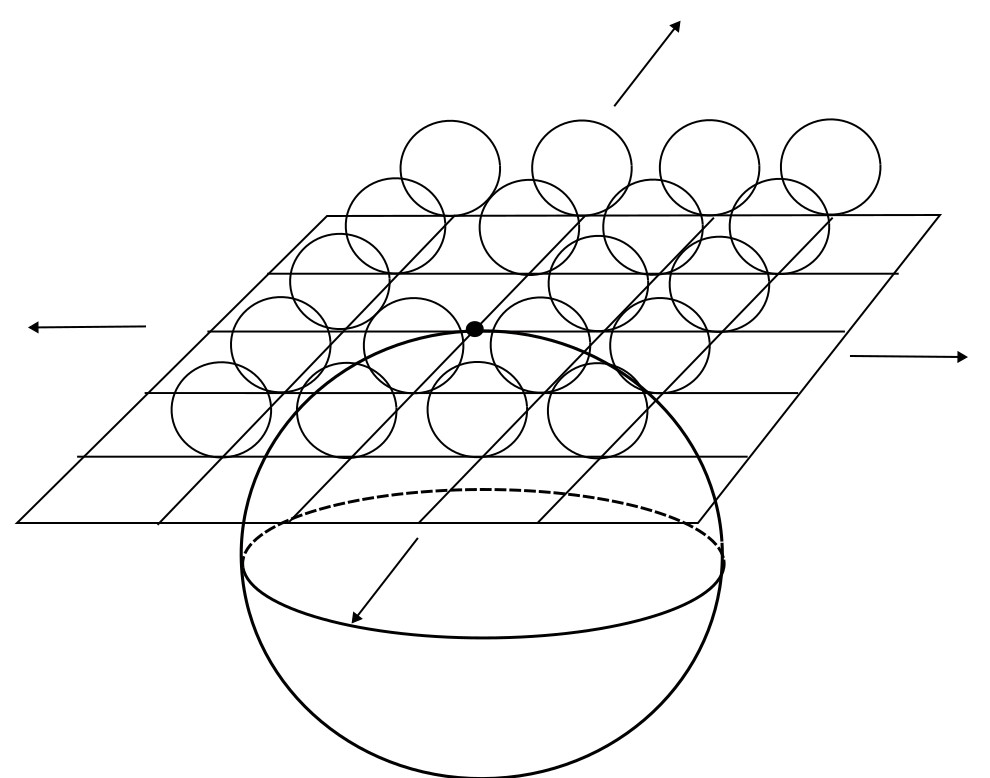
\includegraphics[scale =0.2]{../Graphics/2016AII1_uc.jpg}
	\end{figure}
	
	\begin{prb}{2016-J-I-2}
		Let $X = S^{1} \times S^{1}$ be the 2-torus, and let $Y = X \setminus \{p\}$ be the complement of one point in the 2-torus. \vspace{-0.25cm}
		\begin{enumerate}[itemsep =-2pt,label = (\alph{*})]
			\item Prove that there is no covering map $X \to Y$. 
			\item Prove that there is no covering map $Y \to X$. 
		\end{enumerate}
	\end{prb}
	Let $X = S^{1}\times S^{1}$ denote the 2-torus, and let $Y = X \setminus \{p\}$ be the complement of a point in the 2-torus. \vspace{-0.25cm}
	\begin{enumerate}[itemsep =-2pt,label = (\alph{*})]
		\item Assume to the contrary that there exists a covering map $p: X \to Y$. We first note that $\chi(X) = 2 - 2(1) = 0$. On the other hand, if $B$ is an open ball in $X$ centered at $p$, then by the additivity of the Euler characteristic, one has 
		\begin{equation*}
			0 = \chi(X) = \chi(X \setminus B) + \chi(B) - \chi(S^{1}) = \chi(X \setminus B) + \chi(B) = \chi(Y) + \chi(\{p\}) = \chi(Y) + 1, 
		\end{equation*}
		so that $\chi(Y) = -1$. Since $X$ is assumed to be a compact covering space, the covering must be finitely sheeted. Thus, there exists a finite positive integer $d$ so  that $0 = d \cdot (-1) = -d$, which is a contradiction. Thus by contradiction, there cannot exist such a covering map. 
		
		\item Now assume to the contrary that there is a covering map $p: Y \to X$. Then the induced map $p_{\ast}: \pi_{1}(Y) \to \pi_{1}(X)$ is an injective group homomorphism so that $\pi_{1}(Y)$ is isomorphic to some subgroup of $\pi_{1}(X)$. But since $\pi_{1}(X)$ is abelian, every one of its subgroups is abelian, while $\pi_{1}(Y)$ (the free group on two generators) is nonabelian. Thus by contradiction, $Y$ cannot be a covering space of $X$. 
	\end{enumerate}
	
	\begin{prb}{2015-A-I-1}
		Let $X = \mathbb{RP}^2 \times \mathbb{RP}^2$, where $\mathbb{RP}^2$ denotes the real projective plane. Find all possible connected covering spaces $\ti{X} \to X$ such that $\ti{X}$ is an orientable manifold. 
	\end{prb}
	Let $X$ denote the nonorientable, compact, connected space $\mathbb{RP}^2 \times \mathbb{RP}^2$, where $\mathbb{RP}^2$ is the real projective plane. By the Galois correspondence of covering spaces, the isomorphism classes of connected covering spaces of $X$ are in one-to-one correspondence with the conjugacy classes of subgroups of $\pi_1(X)$. Since $\pi_1(\mathbb{RP}^2) \cong \mathbb{Z}/2\mathbb{Z} \times \mathbb{Z}/2\mathbb{Z}$, there are precisely five subgroups: 
	\begin{enumerate}[itemsep =-2pt,label = (\arabic{*})]
		\item The entire group, $\braket{(0,1),(1,0)}$. If $\ti{X}$ is a connected covering space with fundamental group isomorphic to $\mathbb{Z}/2\mathbb{Z} \times \mathbb{Z}/2\mathbb{Z}$, then the covering map corresponds to the identity map $\operatorname{id}_{X}: X \to X$ so that $\ti{X} = \mathbb{RP}^2 \times \mathbb{RP}^2$, which is a nonorientable cover. 
		\item The trivial subgroup $\{(0,0)\}$, which corresponds to $S^2 \times S^2$, which is an orientable connected manifold. 
		\item The subgroup $\{(0,1), (0,0)\} \cong \{0\} \times \mathbb{Z}/2\mathbb{Z}$, which corresponds to the covering space $S^2 \times \mathbb{RP}^2$, which is nonorientable. 
		\item The subgroup $\{(1,0) \times (0,0)\} \cong \mathbb{Z}/2\mathbb{Z} \times \{0\}$, which corresponds to the covering space $\mathbb{RP}^2 \times S^2$, which is nonorientable. 
		\item The subgroup $\{(0,0),(1,1)\}$. This corresponds with the orientation cover of $X$, and thus is a connected orientable space of $X$. 
	\end{enumerate}
	
	\begin{prb}{2014-A-I-6}
		Let $X$ be a smooth compact manifold whose universal cover is diffeomorphic to an odd-dimensional sphere $S^{2m + 1}$. Show that $X$ is orientable. (Hint:  show that a map  $f: S^{n} \to S^{n}$ without fixed points is homotopic to the antipodal map.) What happens in even dimensions?
	\end{prb}
	Let $X$ be a smooth compact manifold whose universal cover is diffeomorphic to an odd-dimensional sphere $S^{2m + 1}$.  We will use a series of results (as indicated by the hint) to build up our proof. 
		\begin{quote}
			\textbf{Lemma.} (Orientability, Deck Transformations, and Universal Covers) Let $X$ be a smooth compact manifold admitting a universal cover $\hat{p}: \ti{X} \to X$. Let $\Gamma$ denote the group of deck transformations on $\ti{X}$. Then $X \cong \ti{X}/\Gamma$. In particular, $X$ is orientable iff every deck transformation preserves orientation.			
			\textbf{Lemma.} (Uniqueness Property of Deck Transformations) If two deck transformations are equal  at any point $x \in \ti{X}$, then the two transformations are equivalent. In particular, the only deck transformation with a fixed point is the identity transformation. 
			
			\textbf{Lemma.} (Fixed-Point Free Maps on Spheres) Any fixed-point free map $f: S^n \to S^n$ is homotopic to the antipodal map. \vspace{-0.25cm}
			\begin{proof}
				Let $f: S^n \to S^n$ be a fixed-point free map on the $n$-sphere; i.e., for each $x \in S^{n}$, $f(x) \neq x$. Consider the map $H: S^n \times [0,1] \to S^n$ defined by 
				\begin{equation*}
					H(x,t) = \frac{(1 - t)f(x) -tx}{\norm{(1 - t)f(x) - tx}}. 
				\end{equation*}
				By elementary calculus, it is clear to see that $H(x, t)$ is continuous, and hence, a homotopy between $f$ and the antipodal map $\alpha: x \mapsto -x$. 
			\end{proof}
		\end{quote}
	Now we can use these results to prove that $X$ is orientable. By the first lemma, one has that $X \cong S^{2m + 1}/\Gamma$. In particular, $X$ is orientable iff every deck transformation on $S^{2m + 1}$ preserves orientation. Since the identity deck transformation is always orientation preserving, it suffices to check that every \textit{nontrivial} deck transformation preserves orientation. By the second lemma, such nontrivial transformations are necessarily fixed-point free. By the third lemma, such transformations are homotopic to the antipodal map. The degree of the antipodal map, $\alpha: S^{2m + 1} \to S^{2m + 1}$ is $(-1)^{(2m + 1) + 1} = (-1)^{2(m + 1)} = 1$. Since every map of degree 1 preserves orientation, we conclude that every deck transformation on $S^{2m + 1}$ preserves orientation. Thus, $X$ is orientable. However, this result does not generally hold in the even-dimensional sphere case. In particular, one has that the antipodal map in the even-dimensional sphere case is necessarily orientation-reversing. If the group of deck transformations, $\Gamma$, is nontrivial, then necessarily $\Gamma \cong \mathbb{Z}/2\mathbb{Z}$ so that $X \cong S^{2m}/(\mathbb{Z}/2\mathbb{Z}) \cong \mathbb{RP}^{2m}$, which is nonorientable.  
	
	\begin{prb}{2013-A-I-1}
		Use the path lifting property to show the circle is not contractible. Contractible means there is a map of the unit 2-disk into its boundary the unit circle, which is the identity on the boundary. 
	\end{prb}
	Assume to the contrary that there exists a continuous map $f: D^{2} \to S^{1}$ such that $f(x) = x$ for all $x \in S^1$. Since $D^{2}$ is simply connected (and contractible), $\pi_{1}(D^{2}) = 0$ so that the induced map $f_{\ast}: \pi_{1}(D^{2}) \to \pi_{1}(S^{1})$ is trivial. Thus there exists a continuous lift $\ti{f}: D^{2} \to \mathbb{R}$, the universal cover of $S^{1}$, such that $f = p \circ \ti{f}$. Let $\gamma: [0,1] \to S^{1} \subset D^{2}$ be the standard generator loop on the unit circle given by $\gamma(t) = e^{2\pi i t}$. Consider the loop $\ti{\gamma}: [0,1] \to \mathbb{R}$ given by $\ti{\gamma}(t) = \ti{f}(\gamma(t))$. By the path-lifting property, it follows that $\ti{\gamma}(t)$ is the unique lift of $\gamma(t)$ (i.e., $\ti{\gamma}(t) = p(\gamma(t))$). Since the degree of $\gamma$ is 1, it follows that $\ti{\gamma}(1) - \ti{\gamma}(0) = 1 \neq 0$. On the other hand, one has that $\ti{\gamma}(1) = \ti{f}(\gamma(1)) = \ti{f}(\gamma(0)) = \ti{\gamma}(0)$ so that $\ti{\gamma}(1) -\ti{\gamma}(0) = 0$. But this is a contradiction! Thus, no such continuous map $f: D^{2} \to S^{1}$ can exist, which means that the circle is not contractible.  
	
	\begin{prb}{2013-J-II-5}
		If $M$ and $N$ are compact 2-manifolds, their connected sum $M\#N$ is obtained by removing an open disk from each, and then identifying the resulting circle boundaries. It is a theorem that any smooth compact non-orientable surface without boundary is homeomorphic to an iterated connected sum
		\begin{equation*}
			\Sigma_{k} \coloneqq \underbrace{\mathbb{RP}^{2}\#\dotsm \# \mathbb{RP}^{2}}_{k}
		\end{equation*}
		for some positive integer $k$. For which values of $k$ is there a covering map $\Sigma_{k} \to \Sigma_{3}$? 
	\end{prb}
	Let $\Sigma_{3}$ denote the smooth compact non-orientable manifold homeomorphic to  $\mathbb{RP}^{2}\#\dotsm \#\mathbb{RP}^{2}$. Since we are looking for covering spaces $\Sigma_{k}$ (which are compact), it suffices to restrict the search to finite $d$-sheeted covering spaces (infinitely-sheeted covering spaces are necessarily noncompact). If $\Sigma_{k}$ is a covering space of $\Sigma_{3}$, then we must have 
	\begin{align*}
		\begin{split}
			-d = d(3(1) - 2(2)) &= d(3\chi(\mathbb{RP}^{2} - 2\chi(S^{2})) \\
			&= d\cdot \chi(\Sigma_{3}) \\
			&= \chi(\Sigma_{k}) = k\chi(\mathbb{RP}^{2}) + (k - 1)\chi(S^{2}) \\
			&= 2 - k, 
		\end{split}
	\end{align*}
	so that $k = d + 2$. Since $d \geq 1$, we must have $k \geq 3$. On the other hand, suppose $d \geq 1$. Consider the map $\phi: \pi_{1}(\Sigma_{3}) \to \mathbb{Z}/d\mathbb{Z}$, where $\pi_{1}(\Sigma_{3}) \cong \braket{a, b, c \mid a^{2}b^{2}c^{2} = 1}$, defined by 
	\begin{equation*}
		\phi(a) = 1 \qquad \phi(b) = d - 1 \qquad \phi(c) = 0. 
	\end{equation*}
	Then it is clear that $\phi$ is surjective, and that $\phi(a^{2}b^{2}c^{2}) = 0$ so that $\phi$ is a well-defined homomorphism. Thus by the Isomorphism Theorems, $\pi_{1}(\Sigma_{3})/\ker{\varphi} \cong \mathbb{Z}/d\mathbb{Z}$; i.e., $\ker{\varphi}$ is an index $d$ subgroup of $\Sigma_{3}$. By the Galois correspondence of covering spaces, we conclude that $\Sigma_{3}$ must have a $d$-sheeted covering space of genus $g = -d$ so that this covering space is indeed $\Sigma_{d + 2}$. Thus, the values of $k$ for which there is a covering map $\Sigma_{k} \to \Sigma_{3}$ is precisely $k \geq 3$. 
	
	\begin{prb}{2013-J-II-5 (Modified)}
		If $M$ and $N$ are compact 2-manifolds, their connected sum $M\#N$ is obtained by removing an open disk from each, and then identifying the resulting circle boundaries. It is a theorem that any smooth compact non-orientable surface without boundary is homeomorphic to an iterated connected sum
		\begin{equation*}
			\Sigma_{k} \coloneqq \underbrace{\mathbb{RP}^{2}\#\dotsm \# \mathbb{RP}^{2}}_{k}
		\end{equation*}
		for some positive integer $k$. For which values of $k$ is there a covering map $\Sigma_{k} \to \Sigma_{4}$? 
	\end{prb}
	As above, if $\Sigma_{k}$ is a $d$-sheeted covering space ($d \geq 1$) of $\Sigma_{4}$, then we must have 
	\begin{align*}
		\begin{split}
			-2d &= d\cdot\chi(\Sigma_{4}) \\
			&= \chi(\Sigma_{k}) = 2 - k, 
		\end{split}
	\end{align*}
	so that $k =2(d + 1)$. I.e., $k$ is an even integer that is at least $4$. On the other hand, for every $d \geq 1$, there exists a surjective group homomorphism $\varphi: \pi_{1}(\Sigma_{4}) \cong \braket{a, b, c, f\mid a^{2}b^{2}\dotsm f^{2} = 1} \twoheadrightarrow \mathbb{Z}/d\mathbb{Z}$ given by $\varphi(a) = 1$, $\varphi(b)= d- 1$, and $\varphi(c), \varphi(d) = 0$. Since the kernel of this group homomorphism is an index $d$ subgroup of $\pi_{1}(\Sigma_{4})$ (by the First Isomorphism Theorem), we conclude by the Galois correspondence of covering spaces that $\Sigma_{4}$ must have a $d$-sheeted covering space of genus $g = -2d$ so that this covering space is indeed $\Sigma_{2(d + 1)}$. Thus, the values of $k$ for which there is a covering map $\Sigma_{k} \to \Sigma_{3}$ is precisely $\{k \in \mathbb{N} \mid k \text{ even and } k \geq 4\}$. 
	
	\begin{prb}{2010-A-II-4}
		Let $p$ be a prime number. Let $M$ be the two-dimensional torus $S^{1} \times S^{1}$. How many distinct, $p$-sheeted covering spaces $\varpi: \ti{M} \to M$ are there such that $\ti{M}$ is path connected? Count these up to isomorphism of covering spaces of $M$; i.e., $\varpi_{1}: \ti{M}_{1} \to M$ is isomorphic to $\varpi_{2}: \ti{M}_{2} \to M$ if there exists a homeomorphism $f: \ti{M}_{1}  \to \ti{M}_{2}$ such that $\varpi_{2} \circ f = \varpi_{1}$. 
	\end{prb}
	Let $p$ be a fixed prime number, and let $M = S^{1} \times S^{1}$ denote the 2-torus. We note that $M$ is connected and locally simply connected. Then by the Galois correspondence of covering spaces, the isomorphism classes of $p$-sheeted connected covering spaces of $M$ are in one-to-one correspondence with the index $p$-subgroups of $\pi_{1}(M)$. Since $\pi_{1}(S^{1}) \cong \mathbb{Z}$, we have $\pi_{1}(M) \cong \mathbb{Z} \times \mathbb{Z}$. In turn, the number of such subgroups is equivalent to the number of kernels of surjective group homomorphisms: $\phi: \pi_{1}(M) \twoheadrightarrow \mathbb{Z}/p\mathbb{Z}$. We note that $a = (1,0)$ and $b = (0,1)$ are the generators of $\pi_{1}(M)$. Then each homomorphism $\phi: \pi_{1}(M) \to \mathbb{Z}/p\mathbb{Z}$ is uniquely determined by where $\phi$ maps $a$ and $b$. Since $\mathbb{Z}/p\mathbb{Z}$ has $p$ elements, and $a, b$ can be mapped to any one of these elements, it follows that there are a total of $p^{2}$ homomorphisms from $\pi_{1}(M)$ to $\mathbb{Z}/p\mathbb{Z}$. However, a given homomorphism $\phi$ is not surjective if and only if neither $\phi(a)$ nor $\phi(b)$ is a generator of $\mathbb{Z}/p\mathbb{Z}$. Since $p$ is prime, this means that the only non-surjective group homomorphism is the trivial homomorphism. Therefore, there are exactly $p^{2} - 1$ surjective group homomorphisms from $\pi_{1}(M)$ onto $\mathbb{Z}/p\mathbb{Z}$. However, we must also account for the fact that two kernels may be the same up to multiplication by a constant (in which case, the corresponding connected $p$-sheeted covering spaces are isomorphic). Thus, we conclude that, up to isomorphism, there are exactly $(p^{2} - 1)/(p - 1) = p + 1$ $p$-sheeted connected covering spaces of $M$.
	
	\begin{prb}{2005-J-II-5}
		Give an example of a topological space admitting exactly 3 coverings up to equivalence (including the space itself). 
	\end{prb}
	The Galois correspondence of covering spaces tells us that the isomorphism classes of connected covering spaces are in one-to-one correspondence with the conjugacy classes of subgroups of the fundamental group of the base space. Thus, consider e.g. the lens space $L(4;q)$, where $q$ is any positive integer. Since $\pi_1(L(4;q)) \cong \mathbb{Z}/4\mathbb{Z}$, and $\mathbb{Z}/4\mathbb{Z}$ has precisely 3 subgroups ($\{e\}, \{0,2\}, \mathbb{Z}/4\mathbb{Z}$), by the Galois correspondence, $L(4;q)$ must have precisely 3 connected covering spaces up to isomorphism. 
	
	\begin{prb}{2004-A-I-5}
		In this problem, the term ``surface'' means a compact orientable 2-manifold without boundary. \vspace{-0.25cm}
		\begin{enumerate}[itemsep =-2pt,label = (\alph{*})]
			\item Does a surface of genus 1 have a covering space which is homeomorphic to a surface of genus 2? Explain. 
			\item Does a surface of genus 2 have a covering space which is homeomorphic to a surface of genus 3? Explain. 
		\end{enumerate}
	\end{prb}
	\begin{enumerate}[itemsep =-2pt,label = (\alph{*})]
		\item Let $M$ denote a surface of genus 1. We claim that there is no covering space of $M$ that is homeomorphic to a surface of genus 2. Assume to the contrary that there exists a space $\ti{M}$ homeomorphic to a surface of genus 2 that is a $k$-sheeted covering space of $M$ for some finite $k$. Then we must have $\chi_{\ti{M}} = k \cdot \chi_{M}$, where $\chi_{\cdot}$ denotes the Euler characteristic. Since $\chi_{M} = 2- 2(1) = 0$, $\chi_{\ti{M}} = 2 - 2(2) = -2$, and there exists no finite positive integer $k$ so that $-2 = k \cdot 0$, we conclude that $M$ has no finitely-sheeted covering spaces homeomorphic to a surface 2 genus surface. On the other hand, any infinitely-sheeted covering space of $M$ has to be noncompact, and thus cannot be homeomorphic to a (compact) surface of genus 2. 
		\item Now let $M$ denote a surface of genus 2. As above, it suffices to check if there exists a finitely-sheeted covering space of $M$ with genus 3. By looking at the Euler characteristics, \textit{if} $M$ has a finitely-sheeted covering space of genus 3, then it must be a 2-sheeted covering space. But by replicating the work from Problem \ref{prb:2021-A-I-6}, we see that by Galois correspondence of covering spaces, $M$ must have a $2$-sheeted covering space. Thus, we conclude that $M$ has a covering space which is homeomorphic to a surface of genus 2. 
	\end{enumerate}
	
	\begin{prb}{2003-J-II-6}
		Let $M$ be a smooth connected $n$-manifold whose universal cover is diffeomorphic to the $n$-sphere $S^{n}$. \vspace{-0.25cm}
		\begin{enumerate}[itemsep =-2pt,label = (\alph{*})]
			\item Prove the following statement: if $\psi: S^{n} \to S^{n}$ is any diffeomorphism without fixed points, then it is homotopic to the antipodal map. 
			\item Show that if $n$ is odd, then $M$ is orientable. 
			\item Show that if $n$ is even, then $|\pi_{1}(M)| \leq 2$.
		\end{enumerate}
	\end{prb}
	Let $M$ be a smooth connected $n$-manifold whose universal cover is diffeomorphic to the $n$-sphere $S^n$. \vspace{-0.25cm}
	\begin{enumerate}[itemsep =-2pt,label = (\alph{*})]
		\item Let $\psi: S^n \to S^n$ be any diffeomorphism without fixed point (i.e., $\psi(x) - x \neq 0$ for any $x \in S^n$). Then construct the map $H: S^n \times [0,1] \to S^n$ as follows: 
		\begin{equation*}
			H(x,t) = \frac{(1 - t)\psi(x) - tx}{\norm{(1 - t)\psi(x) - tx}}. 
		\end{equation*}
		By calculus arguments, it is clear that $H$ is a homotopy of maps, in particular, a homotopy between $\psi(x)$ and the antipodal map $x \mapsto -x$. 
		\item Suppose $n$ is odd. Since $S^n$ is the universal cover of $M$, one can write $M$ as the quotient $S^n/\Gamma$, where $\Gamma$ is the group of deck transformations on $M$. We note that $M$ is orientable if and only if every deck transformation on $S^n$ is orientation preserving. By (a), every fixed-point free (i.e., nonidentity) deck transformation is homotopic to the antipodal map, $\alpha: S^n \to S^n$. Since the antipodal map has degree $(-1)^{n + 1} = 1$ (since $n + 1$ is even), and the degree is homotopy invariant, one has that every deck transformation is orientation preserving. Thus, we conclude that $M$ is orientable. 
		\item Now assume that $n$ is even. This means that the antipodal map, which has degree $(-1)^{n + 1} = -1$ (since $n + 1$ is odd), is orientation reversing. By (a), every nonidentity deck transformation in $\Gamma$ must be homotopic to the antipodal map, and thus, be orientation reversing. In particular, we notice that for every $\varphi \in \Gamma$, one must have $\varphi^2 = \text{id}$. Thus, one possibility is that $\Gamma = \{e\}$ is the trivial group. But in this case, $M \cong S^{n}$. And since $n$ is even (i.e., $n \geq 2$), $\pi_{1}(M) \cong \pi_{1}(S^{n}) = 0$ since the $n$-sphere, for $n\geq 2$, is simply connected. On the other hand, suppose that $\Gamma$ is not the trivial group. Suppose $\varphi_{1}, \varphi_{2} \in \Gamma$ are nonidentity deck transformations. Then one has $\varphi_1^2 = \text{id} \implies \varphi_{1} = \varphi_{1}^{-1}$ and $\varphi_{1}\circ \varphi_{2} = \text{id} \implies \varphi_{1} = \varphi_{2}^{-1}$. This implies that $\varphi_{2}^{-1} = \varphi_{1}^{-1} \implies \varphi_{1} = \varphi_{2}$. Thus $\Gamma$ contains only one nonidentity element so that $\Gamma \cong \mathbb{Z}/2\mathbb{Z}$. Since $S^{n}$ is simply connected for even $n$ (i.e., $n \geq 2$), it follows that $\pi_{1}(M) \cong \Gamma \cong \mathbb{Z}/2\mathbb{Z}$ so that $|\pi_{1}(M)| = 2$. 
	\end{enumerate}
	
	\begin{prb}{1997-A-I-4}
		Let $S^{n}$ denote the $n$-sphere, and suppose that $f: S^{n} \to S^{n}$ is a continuous map without fixed points. Prove that $f$ is homotopic to the antipodal map $x \mapsto -x$. 
	\end{prb}
	Let $f: S^{n} \to S^{n}$ be a continuous map without fixed points. Define the map $H(x, t): S^{n} \times [0,1] \to S^{n}$ as follows: 
	\begin{equation*}
		H(x,t)= \frac{(1 - t)f(x) - tx}{\norm{(1 - t)f(x) - tx}}. 
	\end{equation*}
	For any $(x, t) \in S^{n} \times [0,1]$, one has that $\norm{H(x, t)} = 1$. Now we need to show that $H$ is well-defined and continuous. The denominator $(1 - t)f(x) - tx$ is equal to zero if and only if $(1  - t)f(x) = tx$. Taking the norm of both sides, one has $1 - t = t \iff t = 1/2$. But at $t = 1/2$, one has that $(1 - t)f(x) - tx = (1/2)(f(x) - x) \neq 0$ since $f(x)$ has no fixed points. This result follows trivially at $t = 0, 1$. Therefore, $H(x, t)$ is well-defined and also continuous. Since $H(x, 0) = f(x)$ and $H(x, 1) = -x$, we conclude that $f$ is homotopic to the antipodal map. 
		
	\subsection{Degree Theory}
	
	\begin{prb}{2020-J-I-2}
		Let $M$ and $N$ be smooth compact connected oriented $n$-manifolds without boundary. Suppose that $\pi_1(M)$ is finite, but that $\pi_1(N)$ is infinite. Prove that every smooth map $\Psi: M \to N$ has degree 0. 
	\end{prb}
	Let $M$ and $N$ be smooth compact connected oriented $n$-manifolds without boundary, and assume that $\pi_1(M)$ is finite, but $\pi_{1}(N)$ is infinite. Let $\Psi: M \to N$ be a smooth map, and assume to the contrary that $\Psi$ has nonzero degree. Then $\Psi_{\ast}(\pi_1(M))$ is a finite-index subgroup of $\pi_1(N)$, and by Lagrange's theorem, this index must divide $\deg{\Psi}$. But since $\pi_{1}(M)$ is finite, $|\Psi_{\ast}(\pi_1(M))|$ is finite, and thus has infinite index in $\pi_1(N)$ (since $|\pi_1(N)|$ is infinite). But this contradicts our hypothesis that $\deg{\Psi} \neq 0$. Thus by contradiction, the proof concludes. 
	
	\begin{prb}{2019-J-I-6}
		Let $T^2$ be a two-dimensional torus and let $f: T^2 \to T^2$ be a continuous map such that the induced map of fundamental groups $f_\ast: \pi_{1}(T^2,x_0) \to \pi_1(T^2, f(x_0))$ is trivial (i.e., the image of $f_\ast$ consists of the identity element). Prove that $f$ has a fixed point. 
	\end{prb}
	Let $T^2$ be a two-dimensional torus,  and let $f: T^2 \to T^2$ be a continuous map such that the induced map of fundamental groups $f_{\ast}: \pi_{1}(T^2, x_0) \to \pi_{1}(T^2, f(x_0))$ is trivial. Assume to the contrary that $f$ has no fixed points. Let $p: \mathbb{R}^{2} \to T^{2}$ be the universal covering space. Let $x_{0} \in T^2$, $y_{0} = f(x_0) \in T^2$, and $\ti{y}_{0} \in \mathbb{R}^2$ such that $p(\ti{y}_{0}) = y_{0}$. Then since $\mathbb{R}^{2}$ is simply connected, one has that 
	\begin{equation*}
		f_{\ast}(\pi_{1}(T^2,x_{0}))  = \{e\} \subset \{e\} = p_{\ast}(\pi_1(\mathbb{R}^2, \ti{y}_0)). 
	\end{equation*}
	Thus there exists a continuous lift, $\ti{f}: T^2 \to \mathbb{R}^2$ such that $f = p \circ \ti{f}$. Since $\mathbb{R}^{2}$ is contractible, $\ti{f}$ must be nulhomotopic. Since homotopies descend from lifts via projections to the base space, $f$ must also be nulhomotopic. This means that the Lefschetz number of $f$, $\Lambda_{f}$, must be: 
	\begin{equation*}
		\Lambda_{f} = \sum_{k \geq 0}(-1)^{k}\operatorname{Tr}\left(f_{\ast,k}: H_{k}(T^{2}; \mathbb{R}) \to H_{k}(T^2; \mathbb{R})\right) = 1 + \sum_{k \geq 1}0 = 1, 
	\end{equation*}
	since the induced maps $f_{\ast,k}$ on homology for $k \geq 1$ are all trivial\footnote{Since $\dim{T^2} = 2$, $H_{k}(T^2; \mathbb{R}) = 0$ for all $k \geq 2$. On the other hand, since $f_{\ast}: \pi_1(T^2) \to \pi_1(T^2)$ is trivial, and $H_1(T^2;\mathbb{R})$ is the abelianization of $\pi_1(T^2)$, $f_{\ast,1}$ must be the trivial map. And since $H_{2}(T^2)$ is generated by products of degree one class, $f_{\ast,2}$ must be the trivial map. For any path connected space $X$, and continuous map $f: X \to X$, the induced map $f_{\ast,0}$ must always be the identity map.} and is the identity on $H_{0}(T^2; \mathbb{R})$. On the other hand, since $f$ has no fixed points, by the Lefschetz-Hopf Theorem, one has that 
	\begin{equation*}
		\Lambda_{f} = \sum_{x \in \operatorname{Fix}{f}}\operatorname{ind}(f,x) = 0, 
	\end{equation*}
	where $\operatorname{Fix}{f}$ denotes the fixed points of $f$, and $\operatorname{ind}(f, x)$ is the fixed-point index. But this is a contradiction! Thus by contradiction, $f$ must have a fixed point. 
	
	\begin{prb}{2018-J-I-5}
		Let $\mathbb{RP}^{n}$ denote the $n$-dimensional real projective space where $n$ is an odd integer. Suppose that a continuous map $f: \mathbb{RP}^{n} \to \mathbb{RP}^{n}$ induces the trivial homomorphism
		\begin{equation*}
			f_{\ast}: \pi_{1}(\mathbb{RP}^{n}, x_{0}) \to \pi_{1}(\mathbb{RP}^{n}, x_{0}). 
		\end{equation*}
		Show that $f$ has a fixed point; i.e., there is $x \in \mathbb{RP}^{n}$ such that $f(x) = x$. 
	\end{prb}
	Let $n$ be an odd integer, and let $f: \mathbb{RP}^{n} \to \mathbb{RP}^{n}$ be a continuous map such that it induces a trivial homomorphism $f_{\ast}$ on fundamental groups. Assume to the contrary that $f$ has no fixed points, and let $p: S^{n} \to \mathbb{RP}^{n}$ denote the universal covering map. Since $f_{\ast}(\pi_{1}(\mathbb{RP}^{n})) \leq p_{\ast}(\pi_{1}(S^{n}))$, there exists a continuous lift $\ti{f}: \mathbb{RP}^{n} \to S^{n}$ of $f$ such that $f = p \circ \ti{f}$. Consider the map $g \coloneqq \ti{f} \circ p: S^{n} \to S^{n}$. Since $f$ is assumed to have no fixed points and $p$ is surjective (by definition of a covering map), for every $x \in S^n$, $f(p(x)) \neq p(x)$. In particular, one has that $p(\ti{f}(p(x))) \neq p(x) \iff p(g(x)) \neq p(x)$ for any $x \in S^{n}$. Since $p(x) = p(-x)$, this implies that $g$ has neither fixed points (i.e., for any $x \in S^{n}$, $g(x) \neq x$) nor antipodal points (i.e., for any $x \in S^{n}$, $g(x) \neq -x$). Since $g(x)$ is a continuous map on $S^{n}$ without fixed points, it is homotopic to the antipodal map, $\alpha: S^{n} \to S^{n}$ which has degree $(-1)^{n + 1} = 1$ since $n$ is odd. However, we also know that $\deg{g} = \deg{\ti{f}} \circ \deg{p} = 2 \cdot \deg{\ti{f}}$ since $p$ is a 2-sheeted covering map. This means that $\deg{g}$ must be even, which is a contradiction! Therefore, by contradiction, we conclude that $f$ must have a fixed point. 
	
	\begin{prb}{2017-A-II-4}
		Let $M$ be a smooth compact connected $n$-manifold (without boundary), and let $\Phi: M\to M$ be a smooth map that is smoothly homotopic to the identity. (In other words, suppose there is a smooth map $F: M \times [0,1] \to M$ such that $F(x,0) = \Phi(x)$ and $F(x,1) = x$ for every $x \in M$.) Show that $\Phi$ must be surjective. 
	\end{prb}
	We will consider two cases for this problem: (1) $M$ is orientable; (2) $M$ is nonorientable. Let $\hat{p}: \hat{M} \to M$ be the orientation cover of $M$. 
	\begin{enumerate}[itemsep =-2pt,label = (\arabic{*})]
		\item Let $M$ be a smooth compact connected oriented $n$-manifold (without boundary), and let $\Phi: M \to M$ be a smooth map that is smoothly homotopic to the identity. Since the degree of the identity map is $1$, and the degree is homotopy invariant, one has that $\deg{\Phi} = 1$. Now we will appeal to the following lemma. 
		\begin{quote}
			\textbf{Lemma.} (Surjectivity and Degree of Smooth Maps) Let $M$ be a smooth compact connected oriented $n$-manifold (without boundary). If $\Phi: M \to M$ is a smooth map with nonzero degree, then $\Phi$ is surjective. \vspace{-0.25cm}
			
			\begin{proof}
				Let $M$ be a smooth compact connected $n$-manifold (without boundary), and let $\Phi: M \to M$ be a smooth map with nonzero degree. Assume to the contrary that $\Phi$ is not surjective. Since $M$ is compact, $\Phi$ must be a proper map, so that $\Phi(M)$ is closed is $M$. Thus, $M \setminus \Phi(M)$ is open. In particular, if $q \notin \Phi(M)$, then there exists an open neighborhood $\ti{U}$ of $q$ in $M$ so that $\ti{U} \subset M \setminus \Phi(M)$. Let $\omega$ be an $n$-form supported in $\ti{U}$ so that $\int_{M}\omega = 1$. Then since $\Phi^{\ast}\omega = 0$ by construction, 
				\begin{equation*}
					\int_{M}\Phi^{\ast}\omega = 0 = 0 \cdot \int_{M}\omega. 
				\end{equation*}
				Since the degree of $\Phi$ is independent of $\omega \in \Omega^{n}(M)$, we conclude that $\deg{\Phi} = 0$, which is a contradiction! Thus, $\Phi$ must be surjective. 
			\end{proof}
		\end{quote}
		So since we have shown that $\Phi$ is a smooth map of degree 1, it follows by the above lemma that $\Phi$ must be surjective. 
		
		\item Let $M$ be a smooth compact connected nonoriented $n$-manifold; by extension, the orientation cover $\hat{M}$ is a smooth compact connected oriented $n$-manifold. Since $\hat{p}$ is a covering map, the smooth homotopy $F: M \times [0,1] \to M$ between $\Phi$ and $\operatorname{id}_{M}$ lifts to a homotopy $\hat{F}: \hat{M} \times [0,1] \to \hat{M}$ between $\hat{\Phi}$ and $\operatorname{id}_{\hat{M}}$, where $\hat{\Phi}(\hat{x}) \coloneqq \hat{F}(\hat{x}, 0)$. By the above lemma in the orientable case, since $\hat{M}$ is orientable, it follows that $\hat{\Phi}: \hat{M} \to \hat{M}$ is surjective. Now fix any $y \in M$, and let $\hat{y} \in \hat{p}^{-1}(y) \subset \hat{M}$. Since $\hat{\Phi}$ is surjective, there exists some $\hat{x} \in \hat{M}$ so that $\hat{\Phi}(\hat{x}) = \hat{y}$. Now recall that $\hat{p} \circ \hat{\Phi} = \Phi \circ \hat{p}$. Thus projecting down the above result to $M$ via $\hat{p}$ gets us 
		\begin{equation*}
			\Phi(\hat{p}(\hat{x})) = \hat{p}(\hat{\Phi}(\hat{x})) = y. 
		\end{equation*}
		Setting $x = \hat{p}(\hat{x}) \in M$, we conclude that there exists some $x \in M$ so that $\Phi(x) = y$. Thus $\Phi$ is surjective. 
	\end{enumerate}
	
	\begin{prb}{2013-A-I-4}
		Two smooth self-maps $f_{0}, f_{1}: S^{n} \to S^{n}$ of the $n$-sphere are said to be smoothly homotopic if there is a smooth map $F: S^{n} \times [0,1] \to S^{n}$ such that $f_{j} = F|_{S^{n}\times \{j\}}$, $j =0, 1$. For which values of $n$ is the antipodal map $\vec{x} \mapsto - \vec{x}$ smoothly homotopic to the identity map of $S^{n}$. Justify your answer with appropriate proofs. 
	\end{prb}
	Let $\alpha: S^{n} \to S^{n}$ denote the antipodal map, $\vec{x} \mapsto -\vec{x}$, and let $i: S^{n} \to S^{n}$ be the antipodal map. We start by noting that the identity map has degree 1 since for any smooth $n$-form on $S^{n}$, 
	\begin{equation*}
		\int_{S^{n}}i^{\ast}\omega = \int_{S}^{n}\omega. 
	\end{equation*}
	On the other hand, we recall that the antipodal map $\alpha$ can be thought of as the composition of $(n + 1)$-reflections; each reflection $(x_{1}, \ldots, x_{i}, \ldots, x_{n + 1}) \mapsto (x_{1}, \ldots, -x_{i}, \ldots, x_{n + 1})$ is an orientation-reversing diffeomorphism, and thus has degree $(-1)$. Since the degree of a composition is the product of the degrees, the antipodal map $\alpha$ has degree $(-1)^{n + 1}$. If $\alpha$ is homotopic to the identity map, then one must have $(-1)^{n + 1} = 1$, so that $n$ is odd. Conversely, suppose $n$ is odd. Let $\{e_{1}, \ldots, e_{n + 1}\}$ be the standard coordinates on $\mathbb{R}^{n}$. We define the following map, $H: S^{n} \times [0,1] \to S^{n}$: 
	\begin{equation*}
		H(x, t) = 
		\begin{pmatrix}
			R(\pi t) & 0 & 0 & \dotsm & 0 & 0\\
			0 & R(\pi t) & 0 & \dotsm & 0  & \vdots \\
			0 & 0 & R(\pi t) & 0 & \dotsm & \vdots \\
			0 & 0 & 0 &  \ddots & 0 & \vdots 
		\end{pmatrix}
		\cdot \begin{pmatrix} x_{1} \\ x_{2} \\ \vdots \\ x_{n + 1} \end{pmatrix}.
	\end{equation*}
	where for each $(x, t) \in S^{n} \times [0,1]$, $H(x,t)$ is an $n \times n$ matrix, and each block entry is the rotation matrix, 
	\begin{equation*}
		R(\pi t) \coloneqq \begin{pmatrix} \cos(\pi t) & -\sin(\pi t) \\ \sin(\pi t) & \cos(\pi t) \end{pmatrix}. 
	\end{equation*}
	Since each of the entries of $R(\pi t)$ is smooth, $H$ is a smooth homotopy between the identity map and the antipodal map. Thus the proof concludes. Alternatively, we could have used the Hopf theorem. 
	\begin{prb}{2001-J-II-1}
		Let $f: M \to N$ be a smooth map between connected smooth compact oriented $n$-manifolds. The degree of $f$ is the number $\deg{f}$ defined by 
		\begin{equation*}
			\int_{M} f^{\ast}\varphi = (\deg{f}) \cdot \int_{N}\varphi, 
		\end{equation*}
		where $\varphi$ is an $n$-form on $N$ whose integral does not vanish. \vspace{-0.25cm}
		\begin{enumerate}[itemsep =-2pt,label = (\alph{*})]
			\item Show that $\deg{f}$ is independent of the choice of $\varphi$, and so depends only on the smooth map $f$. 
			\item Let $X$ and $Y$ be smooth compact oriented manifolds of dimensions $p > 0$ and $q > 0$, respectively, and set $n = p + q$. Show that any map $f: S^{n} \to X \times Y$ has degree 0. 
		\end{enumerate}
	\end{prb}
	\begin{enumerate}[itemsep =-2pt,label = (\alph{*})]
		\item Let $f: M \to N$ be a smooth map between connected smooth compact oriented $n$-manifolds, and assume that for each $\varphi \in \Omega^{n}(N)$ whose integral does not vanish, there exists some real number $k_{\varphi}$ (that depends on $f$ and possibly on $\varphi$) such that 
			\begin{equation*}
				\int_{M}f^{\ast}\varphi = k_{\varphi} \int_{N}\varphi. 
			\end{equation*}
		Fix an arbitrary $\varphi, \ti{\varphi} \in \Omega^{n}(N)$ with non-vanishing integrals on $N$, and define the scaled $n$-form 
		\begin{equation*}
			\ti{\varphi}' = \frac{\int_{N}\varphi}{\int_{N}\ti\varphi}\ti{\varphi}. 
		\end{equation*}
		Then one notices that $\int_{N}\ti{\varphi}' = \int_{N}\varphi$. But by linearity of the pullback map, one has that 
		\begin{equation*}
			k_{\ti\varphi'}\int_{N}\varphi = k_{\ti{\varphi}'}\int_{N}\ti{\varphi'} = \int_{M}f^{\ast}\ti{\varphi}' = k_{\ti\varphi}\int_{N}\varphi. 
		\end{equation*}
		Thus one has that $k_{\ti\varphi'} = k_{\ti\varphi}$. Now since $\int_{N}\varphi = \int_{N}\ti{\varphi}'$, one has that $\int_{N}(\varphi - \ti{\varphi}') = 0$. Since $N$ is a compact connected smooth oriented $n$-manifold, this is possible iff $\varphi$ and $\ti{\varphi}'$ are cohomologous: $\varphi = \ti{\varphi} + d\eta$. But then using Stokes' theorem, since $M$ is without boundary, one gets $\int_{N}f^{\ast}\varphi = \int_{N}f^{\ast}\ti{\varphi}'$. Thus, one gets $k_{\varphi} = k_{\ti\varphi'}$. This forces $k_{\varphi} = k_{\ti{\varphi}}$ so that the proof concludes. 
		\item Now let $X$ and $Y$ be smooth compact oriented manifolds of dimensions $p > 0$ and $q > 0$, respectively, and set $n = p + q$. Let $f: S^{n} \to  X \times Y$ be a smooth map. The top class of $X \times Y$ is a cup product $a \smile b$, where $a \in H^p_{\text{dR}}(X)$ and $b \in H^q_{\text{dR}}(Y)$. Pulling back to $S^n$ the factors land in $H^{p}_{\text{dR}}(S^n)$ and $H^{q}_{\text{dR}}(S^n)$, respectively, But both of these de Rham cohomology groups are zero since $0 < p, q < n$. This means that the pullback of the top class is zero so that the degree of $f$ is also zero. 
	\end{enumerate}
	
	\begin{prb}{2012-A-II-5}
		For a smooth map $f: M \to N$ between smooth, compact, oriented $n$-manifolds, the degree of $f$ is the unique integer $k$ such that 
			\begin{equation*}
				\int_{M}f^{\ast}\omega = k\int_{N}\omega
			\end{equation*}
		for every smooth $n$-form $\omega$ on $N$. Prove or disprove each of the following. \vspace{-0.25cm}
		\begin{enumerate}[itemsep =-2pt,label = (\alph{*})]
			\item There exists a degree-1 smooth map $S^5 \to S^2 \times S^3$. 
			\item There exists a degree-1 smooth map $S^2 \times S^3 \to S^5$. 
		\end{enumerate}
	\end{prb}
	\begin{enumerate}[itemsep =-2pt,label = (\alph{*})]
		\item We claim that this statement is false; let $f: S^{5} \to S^2 \times S^3$ be an arbitrary smooth map. Since $S^2 \times S^3$ is a smooth compact, oriented $n$-manifold, the top de Rham cohomology group $H^{5}_{\text{dR}}(S^2 \times S^3) \cong \mathbb{R}$, and thus the top class is generated by a cup product $\alpha \smile \beta$, where $\alpha \in H^{2}_{\text{dR}}(S^2)$ and $\beta \in H^{3}_{\text{dR}}(S^3)$. Under the pullback map $f^{\ast}$, each of these factors are pulled back to $H^{2}_{\text{dR}}(S^5)$ and $H^{3}_{\text{dR}}(S^{5})$, respectively, both of which are zero. Thus since the pullback of the top class is zero, the degree of $f$ must be zero as well. Since $f$ was arbitrary, the proof concludes. 
		\item This statement is true; see the proof from Problem \ref{prb:2000JI5} for a solution. 
	\end{enumerate}
	
	\begin{prb}{2000-J-I-5}
		If $M$ is any smooth, compact, oriented $n$-manifold, show that there is a smooth map $f: M \to S^n$ with degree 1.
		\label{prb:2000JI5}
	\end{prb}
	Let $M$ be a smooth, connected, compact oriented $n$-manifold, and let $B \subset M$ be a coordinate ball whose orientation agrees with the standard orientation of the unit ball in $\mathbb{R}^n$. Let $\phi: U \to \mathbb{R}^n$ be the corresponding orientation-preserving coordinate chart containing $\overline{B}$ such that $\phi(B) = B_1(0)$, the open unit ball. Let $q: M \to M / (M \setminus B) \cong S^n$ be the natural continuous quotient map that collapses the closed complement $M \setminus B$ to a single basepoint $\infty \in S^n$. This quotient map restricts to a homeomorphism from $B$ onto $S^n \setminus \{\infty\}$. Let $\psi: B_1(0) \to S^n \setminus \{\infty\}$ be a smooth, orientation-preserving diffeomorphism from the unit ball to the punctured sphere. We define an initial continuous map $f_0: M \to S^n$ by setting $f_0(x) = \psi(\phi(x))$ for $x \in B$ and $f_0(x) = \infty$ for $x \in M \setminus B$. To smooth this map, let $\rho: [0, 1] \to [0, 1]$ be a smooth, non-decreasing cut-off function such that $\rho(r) = r$ for $0 \leq r \leq 1/2$ and $\rho(r) = 1$ for $3/4 \leq r \leq 1$. In terms of the radial coordinate $r = \|\phi(x)\|$ on $B$, we define the modified smooth map $f: M \to S^n$ by $f(x) = \infty$ for $x \in M \setminus B$ or for $x \in B$ with $\|\phi(x)\| \geq 3/4$, and $f(x) = \psi\left(\rho(\|\phi(x)\|) \frac{\phi(x)}{\|\phi(x)\|}\right)$ for $x \in B$ with $\|\phi(x)\| < 3/4$. This map $f$ is smooth globally because it is locally constant and equal to $\infty$ on a neighborhood of $M \setminus B$. Now choose a point $y \in S^n \setminus \{\infty\}$ corresponding to a regular value in the image of the inner region where $\|\phi(x)\| < 1/2$. By construction, the preimage $f^{-1}(y)$ consists of exactly one point $x_0 \in B$. Since both $\phi$ and $\psi$ are orientation-preserving and $\rho(r)=r$ on this neighborhood, the differential $df_{x_0}: T_{x_0}M \to T_y S^n$ is a linear isomorphism that preserves orientation. Thus, the local degree at $x_0$ is $+1$. Computing the degree of $f$ by summing the local degrees over the fiber of this regular value yields $\deg(f) = \sum_{x \in f^{-1}(y)} \text{sgn}(\det df_x) = \text{sgn}(\det df_{x_0}) = 1$, completing the proof.
	
	\subsection{Random Manifold Theory}
	\begin{prb}{2020-A-I-6}
		Given a topological space $X$, and a subspace $A \subseteq X$, denote by $X/A$ the space obtained by collapsing $A$ to a point, with the quotient topology. \vspace{-0.25cm}
		\begin{enumerate}[itemsep =-2pt,label = (\alph{*})]
			\item Let $X = S^{1} \times (0,1)$ be a cylinder, and let 
			\begin{equation*}
				A = S^{1} \times \brac*{\frac{1}{2}}
			\end{equation*}
			be the central circle. Prove that $X\setminus A$ is not homeomorphic to a (topological) manifold. 
			\item What happens if instead we take $X$ to be a M\"obius band, and $A$ the center circle? 
		\end{enumerate}
	\end{prb}
	\begin{enumerate}[itemsep =-2pt,label = (\alph{*})]
		\item Consider the following construction. 
			\begin{figure}[h!]
				\centering 
				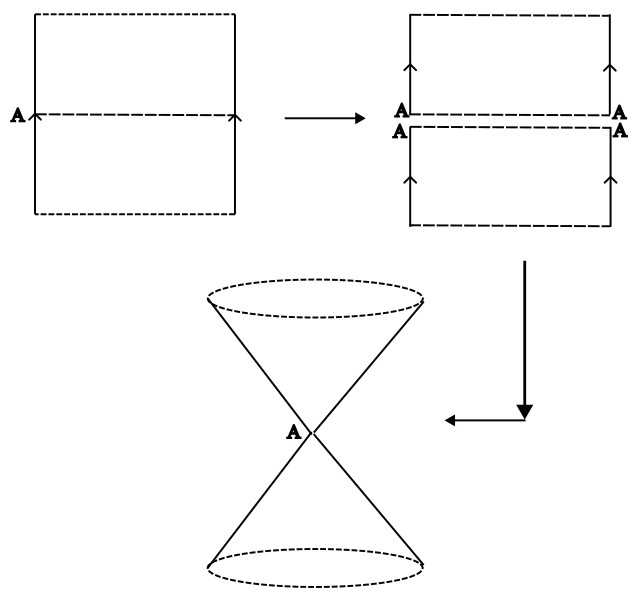
\includegraphics[width = 0.43\textwidth]{../Graphics/2020AI6a.jpg}
			\end{figure}
			
			Then we see that $X/A$ is homeomorphic to the space obtained by taking two cones (minus the bases) and intersecting the two at their tips. Let $p = [A] \in X/A$, and assume that $X/A$ were homeomorphic to a topological manifold. Then there must exist an open neighborhood $U$ of $p$ in $X\setminus A$ such that $U$ is homeomorphic to an open disk in $\mathbb{R}^{2}$. But $U \setminus \{p\}$ must have at least two connected components, while the complement of a single point in an open disk is still connected. Since the number of connected components is preserved under homeomorphsms, we have reached a contradiction. Thus, $X/A$ is not homeomorphic to a manifold. 
			
		\item Now consider the following construction. 
		
		\begin{figure}[h!]
			\centering 
			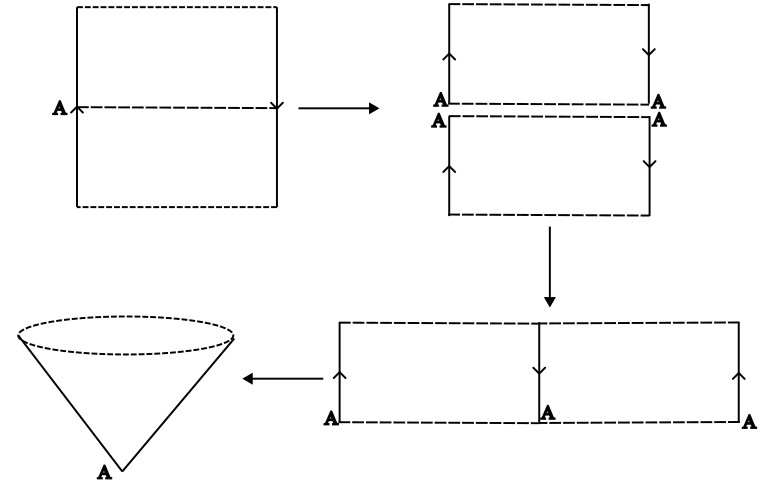
\includegraphics[width=\textwidth]{../Graphics/2020AI6b.jpg}
		\end{figure}
		
		In this case, we see that $X/A$ is homeomorphic to a cone; $X/A$ is homeomorphic to the disk by means of the projection map from $X/A$ to $\mathbb{R}^{2}$ (e.g., the map $f: (x, y, z) \in C \mapsto (x, y)$, where $C$ denotes the 2-dimensional cone embedded in $\mathbb{R}^{3}$). Since the disk is a topological 2-manifold, we conclude that $X/A$ is homeomorphic to a topological manifold when $X$ is the M\"obius band, and $A$ is the center circle. 
	\end{enumerate}
	
	\begin{prb}{2009-J-I-1}
		Let $M^{k}$ be a smooth compact $k$-manifold, and let $F: M \to S^{n}$ be a smooth map, where $n > k$. Prove that $F$ is homotopic to a constant map. 
	\end{prb}
	Let $M^{k}$ be a smooth compact $k$-manifold, and let $F: M \to S^{n}$ be a smooth map, where $n > k$. In particular, this implies that for any $x \in M$, $dF_{x}: T_{x}M \to T_{F(x)}S^{n}$ is not surjective so that every point in $F(M)$ is a critical value. By Sard's Theorem, this implies that $F(M)$ is a measure zero subset of $S^{n}$. Therefore, there exists at least one $q \in S^{n}$ such that $F(M) \subseteq S^{n}\setminus \{q\}$. Thus one can view $F$ as a map from $M$ to $S^{n}\setminus \{q\}$, which is contractible as it is homeomorphic to $\mathbb{R}^{n}$. Since any smooth map into a contractible space is nulhomotopic, we conclude that $F$ is nulhomotopic (i.e., homotopic to a constant map). 	
	\newpage
	\section{Algebra}
	
	\subsection{Ring Theory}
	
	\begin{prb}{2025-J-I-1}
		Let $R$ be a UFD (unique factorization domain). Let $F$ be its quotient field. Let 
		\begin{equation*}
			p(x) = x^{n} + b_{n-1}x^{n - 1} + \dotsm + b_{0} \in F[x]
		\end{equation*}
		be a monic polynomial with coefficients in $R$ admitting a root $a \in F$. Prove that $a \in R$. 
	\end{prb}
	Let $R$ be a UFD, and let $F$ denote its quotient field. Let $p(x)$ be the aforementioned monic polynomial in $F[x]$. Furthermore, assume $a = b/c$, with $b, c \in R$, $c \neq 0$, and $\gcd(b, c) = 1$ (the last assumption is well-defined since (1) for any two elements in a UFD, the greatest common divisor is defined, and (2) if $\gcd(b, c) \neq 1$, then we can reduce the quotient repeatedly until this property is satisfied). Then plugging in $a = b/c$ into $p(x)$, one obtains: 
	\begin{equation*}
		\frac{b^{n}}{c^{n}} + b_{n-1}\frac{b^{n-1}}{c^{n-1}} + \dotsm + b_{1}\frac{b}{c} + b_{0} = 0, 
	\end{equation*}
	which then implies that 
	\begin{equation*}
		b^{n} + b_{n-1}b^{n-1}c + \dotsm + b_{1}bc^{n-1} + b_{0}c^{n} = 0 \implies b^{n} = -c(b_{n-1}b^{n-1} + b_{n-2}b^{n-2}c^{2} + \dotsm + b_{0}c^{n-1}),
	\end{equation*}
	where $(b_{n-1}b^{n-1} + b_{n-2}b^{n-2}c^{2} + \dotsm + b_{0}c^{n-1}) \in R$. Thus, it follows that $c \mid b^{n}$. Since $\gcd(b, c) = 1$, $\gcd(b^{n}, c) = 1$ since raising $b$ to the $n$th power does not add any new prime divisors. Thus since $c \mid b^{n}$ and $\gcd(b^{n}, c) = 1$, $c = \pm 1$. This implies that $a = \pm b \in R$. Hence, the proof concludes. 
	
	
	\begin{prb}{2024-J-I-4}
		For each field $K$, prove that the polynomial ring $K[x,y]$ in two variables is not a principal ideal domain. 
	\end{prb}
	Let $K$ be an arbitrary field, and consider the polynomial ring $K[x,y]$ in two variables. It suffices to show that there exists an ideal of $K[x,y]$ that is not principal. Consider the ideal $(x, y)$. First, we claim that $(x,y)$ is not proper. Every polynomial in $(x,y)$ is of the form $a(x,y)\cdot x + b(x,y) \cdot y$. In particular, at the origin $(x,y) = (0,0)$, one has that every polynomial in the ideal vanishes. But this means that the constant polynomial $1$ cannot be a part of $(x,y)$. Now assume to the contrary that $(x, y)$ is principal: $(c) = (x, y)$. Since $c$ must be a divisor of both $x$ and $y$, and $x, y$ are coprime, $c$ must be a unit. But this implies that $(c) = K[x,y]$ so that $(x,y)$ is the whole polynomial ring; we explicitly showed that this was not the case. Thus by contradiction, it follows that $(x,y)$ is not principle, and so $K[x,y]$ is not a principal ideal domain. 
	
	\begin{prb}{2021-J-II-1}
		Let $R$ denote the product of countably many copies of the field $\mathbb{F}_{2}$ with two elements. $R$ is a commutative ring in which addition and multiplication are defined coordinatewise. If $P \subset R$ is a prime ideal, then verify that the quotient ring $R/P$ is a field, and find the cardinality of this field. 
	\end{prb}
	Let $R$ denote the product of countably many copies of the field $\mathbb{F}_{2}$. Note that for any $x \in \mathbb{F}_{2}$, $x^{2} = x$. Since multiplication is defined pointwise in $R$, for any $a \in R$, $a^{2} = a$. Thus assume $a + P \in R/P$. Then, one has that 
	\begin{equation*}
		(a + P)^{2} = a^{2} + P = a + P \implies a(a - 1) + P = P. 
	\end{equation*}
	Thus one has that $a(a - 1) \in P$. Since $P$ is a prime ideal, either $a \in P$ (in which case $a + P = 0 + P$ or $a - 1 \in P$ so that $a + P = 1 + P$). Thus since $R/P$ is an integral domain (because $P$ is prime) that contains only two elements, and $R/P$ inherits the additive and multiplicative properties of a field by virtue of being a quotient ring, we conclude that $R/P$ is a field. Consequently, the cardinality is 2. 
	
	\begin{prb}{2020-J-I-5}
		Let $\mathbb{K}$ be a field, and let $\mathbb{K}[x]$ be the ring of polynomials in $\mathbb{K}$. Let $\mathscr{I} \subsetneq \mathbb{K}[x]$ be a maximal ideal. Show there is some irreducible polynomial $p(x) \in \mathbb{K}[x]$ such that $\mathscr{I} = \{q(x)p(x): q(x) \in \mathbb{K}[x]\}$. 
	\end{prb}
	Let $\mathbb{K}[x]$ be a field, and let $\mathbb{K}[x]$ be the ring of polynomials in $\mathbb{K}$. Since $\mathbb{K}$ is a field, it follows that the polynomial ring is a principal ideal domain (PID), so that there exists some $p(x) \in \mathbb{K}[x]$ such that $\mathscr{I} = (p(x)) = \{q(x)p(x): q(x) \in \mathbb{K}[x]\}$. Assume to the contrary that $p(x)$ is reducible over $\mathbb{K}$, and let $p_{1}(x) \dotsm p_{n}(x)$ be a factorization of $p(x)$ into irreducible factors. Up to relabeling of the indices, assume that $p_{1}(x)$ is the lowest-degree nonconstant irreducible divisor of $p(x)$. Since $p_{1}(x)$ is a nonconstant polynomial, $(p_{1}(x))$ is a proper ideal of $\mathbb{K}[x]$. By definition, this means $(p_{1}(x)) \supset \mathscr{I}$. On the other hand, since $p(x) \nmid p_{1}(x)$ (because $\deg{p_{1}(x)} < \deg{p(x)}$) $(p_{1}(x)) \not \subset \mathscr{I}$. This contradicts maximality of $\mathscr{I}$. Thus by contradiction, $p(x)$ must be irreducible. The proof concludes. 
	
	\begin{prb}{2019-A-II-6}
		Let $R$ be a commutative ring with identity. \vspace{-0.25cm}
		\begin{enumerate}[itemsep =-2pt,label = (\alph{*})]
			\item Let $P$ be a prime ideal of $R$. Suppose $I_{1}$ and $I_{2}$ are two other ideals of $R$. If $I_{1} \cap I_{2} \subset P$, show that either $I_{1} \subset P$ or $I_{2} \subset P$. 
			\item Suppose that $R$ satisfies the condition that for any decreasing sequence $I_{1} \supset I_{2} \supset I_{3} \supset \dotsm$ of ideals in $R$, there exists an $N$ such that $I_{n}=   I_{N}$ for all $n\geq N$. Show that $R$ has only finitely many maximal ideals. 
		\end{enumerate}
	\end{prb}
	Let $R$ be a commutative ring with identity, $P$ a prime ideal of $R$, and $I_{1,2}$ any two other ideals of $R$. \vspace{-0.25cm}
	\begin{enumerate}[itemsep =-2pt,label = (\alph{*})]
		\item Assume to the contrary that neither $I_{1} \subset P$ nor $I_{2} \subset P$. Then we can find elements $g \in I_{1} \setminus P$ and $h \in I_2 \setminus P$. Since ideals are closed under multiplication by elements in $R$, $gh \in I_{1} \cap I_{2} \subset P$. But since $P$ is a prime ideal, one must have that $g \in P$ or $h \in P$, which is a contradiction! Thus by contradiction, at least one of $I_{1}, I_{2}$ must be entirely contained in $P$. 
		\item Suppose now that $R$ satisfies the descending chain condition for ideals; i.e., assume that for any decreasing sequence $I_{1} \supset I_{2} \supset I_{3} \supset \dotsm$ of ideals in $R$, there exists an $N$ such that $I_{n}= I_{N}$ for all $n \geq N$. Assume to the contrary that $R$ contains infinitely many distinct maximal ideals $\{M_{j}\}_{j = 1}^{\infty}$. For each $n \in \mathbb{N}$, define the ideal 
f2		\begin{equation*}
			I_{n} = \bigcap_{j = 1}^{n}M_{j} \subset R. 
		\end{equation*}
		This gives us a decreasing sequence of ideals $\{I_{n}\}_{n = 1}^{\infty}$ in $R$. By the hypothesis on $R$, there exists some $N > 0$ such that for all $n \geq N$, $I_{n} = I_{N}$. In particular, one has that 
		\begin{equation*}
			I_{N} = M_{1} \cap M_{2} \cap \dotsm \cap M_{N} = I_{N + 1} \subseteq M_{N + 1}. 
		\end{equation*}
		Since every maximal ideal is prime (by definition), using the result of (a) shows that at least one of $M_{1}, M_{2}, \ldots, M_{N}$ is contained in $M_{N + 1}$. But this contradicts our hypothesis that the $\{M_{j}\}_{j = 1}^{\infty}$ were distinct \textit{maximal} ideals. Thus by contradiction, $R$ can only have finitely many distinct maximal ideals. 
	\end{enumerate}
	
	\begin{prb}{2019-J-II-2}
		Does there exist an integral domain with exactly 2019 prime ideals? 
	\end{prb}
	We claim that there does exist an integral domain with exactly 2019 prime ideals. Consider the polynomial ring $\mathbb{Q}[x]$. Since $\mathbb{Q}$ is a field (and hence, an integral domain), one has that $\mathbb{Q}[x]$ is an integral domain; $\mathbb{Q}[x]$ already has at least one prime ideal (namely the zero ideal $(0)$). Pick 2018 irreducible elements from $\mathbb{Q}[x]$; e.g., let $p_{j}(x) = (x - j) \in \mathbb{Q}[x]$ for $j = 1, 2, \ldots, 2018$. Now define 
	\begin{equation*}
		R \coloneqq 
		\brac*{\frac{f(x)}{g(x)} : f(x), g(x)\in \mathbb{Q}[x], p_{j}(x) \nmid g(x) \quad \forall 1 \leq j \leq 2018}. 
	\end{equation*}
	It is straightforward to see that $R$ is nonempty (e.g., $R$ contains the constant polynomial $1 \in \mathbb{Q}[x]$). Next, one has that for any $f(x)/g(x), h(x)/k(x) \in R$, 
	\begin{equation*}
		\frac{f(x)}{g(x)} - \frac{h(x)}{k(x)} = \frac{f(x)k(x) - h(x)g(x)}{g(x)k(x)} \in R
	\end{equation*}
	because $p_{j}(x) \nmid g(x), k(x)$ for any $1 \leq j \leq 2018$ implies $p_{j}(x) \nmid g(x)k(x)$ for any $j$, and the numerator is immediately seen to be in $\mathbb{Q}[x]$. Likewise, we can show that $R$ is closed under multiplication. Hence, $R$ is a subring of $\mathbb{Q}[x]$. In particular, $R$ must be an integral domain as $\mathbb{Q}[x]$ is an integral domain. Consider the ideals $(p_{j}(x))$ for each $j = 1, \ldots, 2018$. Let $f(x)/g(x), h(x)/k(x) \in R$ be arbitrary elements, and assume that for some $j \in \{1, \ldots, 2018\}$, $p_{j}(x) \mid (f(x)h(x))/(g(x)k(x))$. In particular, it follows that $p_{j}(x) \mid f(x)h(x)$. But since $\mathbb{Q}[x]$ is a principal ideal domain (since $\mathbb{Q}$ is a field), it follows that $p_{j}(x)$ divides $f(x)$ or $h(x)$, and thus divides $f(x)/g(x)$ or $h(x)/k(x)$. This shows that $(p_{j}(x))$ is a prime ideal for each $1 \leq j \leq 2018$. This shows that $R$ has at least 2019 prime ideals. Assume to the contrary that there exists a nonzero prime ideal $P$ that is not one of the prime ideals we stated above. Then $P$ contains some nonzero element $f(x)/g(x)$. In particular, $g(x)$ is a unit in $R$, which implies $f(x) \in P$. Factor $f(x)$ into a product of irreducible polynomials, $f(x) = c \cdot q_{1}(x) \cdot \dotsm q_{N}(x)$. Since $P$ is prime, there exists some $q_{i_{0}}(x)$ so that $q_{i_{0}}(x) \in I$. If $q_{i_{0}}(x)$ is not one of the above mentioned irreducible elements, then it follows that $q_{i_{0}}(x)$ is a unit in $R$. But then $P$ contains a unit, and thus must be the whole ring (contradicting our hypothesis that $P$ is proper). Thus $P$ cannot be a prime ideal, and $R$ has exactly 2019 prime ideals.
	
	\begin{prb}{2018-A-I-1}
		For which primes $p \in\mathbb{Z}_{+}$ is $\braket{x^{2} -x + 1, p}$ a prime ideal of $\mathbb{Z}[x]$. 
	\end{prb}
	We recall that if $R$ is a commutative ring with identity, $R/I$ is an integral domain if and only if $I$ is a prime ideal in $R$. Thus the problem reduces to finding all such primes $p \geq 2$ for which $\mathbb{Z}[x]/\braket{x^{2} - x + 1, p}$ is an integral domain. We begin by noticing that 
	\begin{equation*}
		\mathbb{Z}[x]/\braket{x^{2} - x + 1, p} \cong \mathbb{F}_{p}[x]/\braket{x^{2} - x + 1}, 
	\end{equation*}
	where $\mathbb{F}_{p}$ denotes the finite field with $p$ elements. Consequently, $\mathbb{F}_{p}[x]$ is a PID. Since in a PID a nonzero principal ideal is prime if and only if the generator of the ideal is irreducible, our task further reduces to finding those values of prime $p$ such that $p(x) = x^{2} - x + 1$ is irreducible over $\mathbb{F}_{p}$. One notices immediately that $p(x)$ is irreducible over $\mathbb{F}_{2}$ as it has no roots. Now suppose $p > 2$. Consider the polynomial $q(x) = x^{3} + 1 = (x^{2} -x + 1)(x + 1)$. If $p(x)$ has a root, then $q(x)$ must also have a root in $\mathbb{F}_{p}[x]$. Notice that a root of $p(x)$ must therefore satisfy the relation $x^{3} = -1 \pmod{p}$. In particular, since $6$ is the smallest positive exponent of a root of $p(x)$ so that the power yields the identity, every root of $p(x)$ has order 6 in $\mathbb{F}_{p}^{\times}$. But since $\mathbb{F}_{p}^{\times}$ has order $p - 1$, by Lagrange's theorem, one requires $6 \mid (p - 1)$, or $p - 1 = (2k) \cdot 3 = m \cdot 3$ for some $m \in \mathbb{Z}$. Thus $p \equiv 1 \pmod{3}$. Consequently, if $p$ is any prime such that $p \equiv 2 \pmod{3}$, then $p(x)$ is irreducible over $\mathbb{F}_{p}$. Therefore, we conclude that $\braket{x^{2} - x + 1, p}$ is a prime ideal of $\mathbb{Z}[x]$ iff $p$ is a positive prime integer satisfying $p \equiv 2 \pmod{3}$. 
	
	\begin{prb}{2016-J-I-6}
		Prove that the ring $\mathbb{C}[x,y,z]/\braket{y^{2} - xz, x^{3} - yz}$ is not a UFD. 
	\end{prb}
	Let $R \coloneqq \mathbb{C}[x,y,z]/\braket{y^{2} - xz, x^{3} - yz}$, and let bars denote the classes in $R$. Consider the class $q = \bar{z}^2 - \bar{x}^2\bar{y}$. Then one computes in $R$, 
	\begin{equation*}
		\bar{x}q = \bar{x}\bar{z}^2 - \bar{x}^3\bar{y} = \bar{x}\bar{z}^{2} - \bar{y}^{2}\bar{z} = \bar{y}^{2}\bar{z} - \bar{y}^{2}\bar{z} = 0. 
	\end{equation*}
	We claim that neither of these classes are zero. The class $\bar{x}$ is nonzero since the point $(1,1,1)$ satisfies both of the modded relations but $x(1,1,1) = 1$. Likewise, $q$ is nonzero since the point $(0,0,1)$ satisfies the modded relations, but $q(0,0,1) = 1$. Thus since $R$ has nonzero zero divisors, it cannot be an integral domain, and hence, surely not a UFD. 
	
	\begin{prb}{2015-J-II-1}
		Prove that ring $\mathbb{Z}[x,y]/\braket{x^{5} - y^{3}}$ is not a unique factorization domain. 
	\end{prb}
	Let $R \coloneqq \mathbb{Z}[x,y]/\braket{x^{5} - y^{3}}$, and let bars denote the classes in $R$. One has that the class $\bar{y}$ is irreducible. Since in a UFD, ideals are prime iff they are irreducible, $\braket{y}$ is prime. Thus, 
	\begin{equation*}
		\mathbb{Z}[x,y]/\braket{x^{5} - y^{3}}/\braket{y} \cong \mathbb{Z}[x,y]/\braket{x^{5}} 
	\end{equation*}
	must be an integral domain. But this is a contradiction since the two classes $\bar{x}^{4} \cdot \bar{x} = 0$ and neither of these classes are nonzero.
	
	\begin{prb}{2014-A-I-4}
		Prove that the tensor product $\mathbb{C} \otimes_{R} \mathbb{C}$ is not an integral domain. 
	\end{prb} 
	We will tackle this problem in two ways. \vspace{-0.25cm}
	\begin{enumerate}[itemsep =-2pt,label = (\arabic{*})]
		\item (\textsc{Explicit Construction}) Consider the tensors $r = (1 \otimes 1) - (i \otimes i)$ and $s = (1 \otimes 1) + (i \otimes i)$. Then one has that 
		\begin{align*}
			\begin{split}
				rs &= \left[(1 \otimes 1) - (i \otimes i)] \cdot [(1 \otimes 1) + (i \otimes i)\right] \\
				&= (1 \otimes 1) + (i \otimes i) - (i \otimes i) - (1 \otimes 1) \\
				&= (0 \otimes 0)= 0. 
			\end{split}
		\end{align*}
		Since neither $r$ nor $s$ are zero tensors, we conclude that $\mathbb{C} \otimes_{\mathbb{R}} \mathbb{C}$ is not an integral domain as it contains zero divisors. 
		\item (\textsc{Abstract Methodology}) Recall that $\mathbb{C} \cong \mathbb{R}[x]/(x^{2} + 1)$. Thus 
		\begin{equation*}
			\mathbb{C} \otimes_{\mathbb{R}}\mathbb{C} \cong \mathbb{C} \otimes_{\mathbb{R}}\frac{\mathbb{R}[x]}{(x^{2}  + 1)} \cong \frac{\mathbb{C}[x]}{(x^{2} + 1)} \cong \mathbb{C} \times \mathbb{C}. 
		\end{equation*}
		The latter is not an integral domain, as it contains nonzero elements $(1,0)$ and $(0,1)$ such that their product is identically zero. 
	\end{enumerate}
	
	\begin{prb}{2014-J-I-2}
		$R$ is a ring with $1 \neq 0$ and no zero divisors. Suppose that every descending sequence $I_{1} \supset I_{2} \supset \dotsm$ of left ideals in $R$ is eventually constant: that is, $I_{j} = I_{i}$ whenever $i, j$ are sufficiently large. Prove that $R$ is a division ring. 
	\end{prb}
	Let $R$ be a ring with $1 \neq 0$, and no zero divisors. Further assume that $R$ satisfies the descending chain condition for left ideals. Assume to the contrary that $R$ is not a division ring; i.e., assume there exists a nonzero element $a \in R$ such that $a$ has no multiplicative inverses (i.e., is a nonunit). Consider the ideal $Ra$ in $R$. Since $a \in R$, the element $a^2 \in Ra$ such that $Ra^2 \subseteq Ra$. In this way, for each $n \in \mathbb{N}$, define $I_{n}= Ra^{n}$. This gives us a sequence $\{I_{n}\}_{n = 1}^{\infty}$ of decreasing ideals in $R$. By the decreasing chain condition on left ideals in $R$, there exists some $N > 0$ such that for all $n \geq N$, $I_{n} = I_{N}$. In particular, one has that $I_{N} = I_{N + 1} \iff Ra^{N} = Ra^{N + 1}$. This means there exists some $r \in R$ such that $a^{N} = ra^{N + 1} = (ra)a^{N}$. Subtracting, one has $(1 - ra)a^{N} = 0$. Since $R$ has no zero divisors, $a^{N} \neq 0$. Thus, one must have that $1 - ra = 0 \iff ra = 1$; i.e., $a$ must have a left inverse. Now we note that 
	\begin{equation*}
		(ar - 1)a = a(ra) - a = a - a = 0. 
	\end{equation*}
	And since $a \neq 0$ and $R$ has no zero divisors, one must have $ar = 1$. Thus $r$ is a multiplicative inverse of $a$, which contradicts our hypothesis that $a$ is not a unit. Thus it follows that every nonzero element in $R$ has a multiplicative inverse so that $R$ is a division ring. If $R$ were commutative, then $R$ would be a field. 
	
	\begin{prb}{2006-A-I-5}
		Let $R$ be an integral domain. Show that $R$ is a UFD iff every ascending chain of principal ideals stabilizes, and every irreducible element of $R$ is prime. [Recall: $a$ is irreducible iff $a = xy$ implies that either $x$ or $y$ is invertible; $a$ is prime iff $a \mid xy$ implies that $a \mid x$ or $a \mid y$.]
	\end{prb}
	Let $R$ be an integral domain. 
	
	($\Longleftarrow$) Let $R$ be an integral domain satisfying the ascending chain condition on principal ideals (ACCP), and further assume that every irreducible element in $R$ is prime. Assume to the contrary that $R$ is not a UFD. This implies that there exists at least one nonzero noninvertible element $x_{0} \in R$ such that $x_{0}$ does not split into a product of finitely many irreducible elements (notably, $x_{0}$ itself cannot be irreducible). Thus $x_{0}$ must split into a product of nonzero nonunit factors, at least one of which (denoted by $x_1$) must also not split into a product of finitely many irreducible elements. Repeating the argument for $x_0$, we obtain yet another element $x_2$ dividing $x_1$ that does not split into a product of finitely many irreducible elements. Repeating this procedure indefinitely, we obtain an infinite sequence $\{x_{j}\}_{j = 0}^{\infty}$ of elements of $R$ that do not split into a product of finitely many irreducible elements. For each $j \geq 0$, consider the principal ideal $I_{j} = Rx_{j}$ in $R$. Since the sequence of $x_j$ extends indefinitely, the sequence of principal ideals is a strictly ascending chain. By the ACCP hypothesis on $R$, there exists some finite $N > 0$ such that for all $n \geq N$, $I_{n} = I_{N}$. But this contradicts our claim that the chain is strictly ascending. Thus by contradiction, it follows that every nonzero noninvertible element $x_{0} \in R$ must split into the product of finitely many irreducible elements. Now we will show uniqueness of this factorization. Fix a nonzero nonunit element $x \in R$, and assume that $x$ has the factorizations, $p_{1}p_{2}\dotsm p_{n} = x = \ti{p}_{1}\ti{p}_{2}\dotsm \ti{p}_{m}$, where $n, m \geq 1$, and each $p_{i}, \ti{p}_{j}$ is an irreducible element in $R$. Assume without loss of generality that $m > n$. By our hypothesis for irreducible elements in $R$, since $p_{1} \mid \ti{p}_{1}\ti{p}_{2}\dotsm \ti{p}_{m}$, $p_{1}$ must divide one of these irreducible elements. Possibly after relabeling, suppose $p_{1} \mid \ti{p}_{1}$. Since $\ti{p}_{1}$ is irreducible, there exists a unit $u_{1} \in R$ such that $\ti{p}_{1} = u_{1} p_{1}$. Thus one has that $p_{1}p_{2}\dotsm p_{n} = u_{1}p_{1}\ti{p}_{2}\dotsm \ti{p}_{m}$. Since $R$ is an integral domain, the cancellation law yields $p_{2}\dotsm p_{n} = u_{1}\ti{p}_{2}\dotsm \ti{p}_{m}$. Thus now, possibly after relabeling the indices, $p_{2}$ divides $\ti{p}_{2}$. Repeating the same argument as before and inducting on $p_{i}$ ($i = 1, \ldots, n$), one ultimately obtains $1 = u_{1}u_{2}\dotsm u_{n}\ti{p}_{n + 1}\dotsm \ti{p}_{m}$, where $u_{1}\dotsm u_{n}$ is a unit in $R$ as it is the finite product of units. But since this implies $1 = u \cdot \ti{p}_{n + 1} \dotsm \ti{p}_{m}$, we have that $\ti{p}_{n + 1}\dotsm\ti{p}_{m}$ must be a unit in $R$, which is a contradiction since the finite product of irreducible elements cannot be a unit. Thus, we obtain $m = n$. And moreover, we have shown that the two factorizations of $x$ differ by a unit. Therefore, since we have shown that every nonzero nonunit element of $R$ has a unique (up to units) factorization into a product of finitely many irreducible elements, we conclude that $R$ is a UFD. 
	
	($\Longrightarrow$) Now assume that $R$ is a UFD. First we will show that every ascending chain of principal ideals stabilizes. Consider the ascending chain $(x_{1}) \subsetneq (x_{2}) \subsetneq (x_{3}) \subsetneq \dotsm$. Since $R$ is a UFD, there exists a unique (up to units) factorization of $x_{1}$, $x_{1} = p_{1}p_{2}\dotsm p_{m}$, into a finite product of irreducible elements $p_{1}, \ldots, p_{m}$ in $R$. Since $x_{2}$ is a proper factor of $x_{1}$ (proper in the sense that $x_{2}$ is neither a unit nor an associate of $x_{1}$), the number of irreducible factors of $x_{2}$ (counting multiplicity) must be strictly less than $m$. Likewise, since $x_{3}$ is a proper factor of $x_{2}$ (in the same sense of ``proper''), the number of irreducible factors of $x_{3}$ (counting multiplicity) must be strictly less than that of $x_{2}$. Thus since every decreasing sequence of nonnegative integers must terminate, we find that the chain of ascending ideals must terminate after at most $m$ steps (at which point, the generator is either a unit or an associate of an irreducible element). Thus since this chain was arbitrary, we have shown that every ascending chain of principal ideals stabilizes. Now we will show that every irreducible element is prime. Let $p \in R$ be an arbitrary irreducible element and assume that $p \mid xy$ for some $x, y \in R$. Then there exists some $c \in R$ such that $pc = xy$. Since $R$ is a UFD, there exist unique (up to units) factorizations of $x, y, c$ into irreducible elements. Suppose $x = p_{1}\dotsm p_{m}$, $y = q_{1}\dotsm q_{n}$, and $c = r_{1}\dotsm r_{s}$. Substituting these factorizations back into the original equation, by unique factorization in $R$, it follows that $p$ must be equal to one of the irreducible factors of $a$ or $b$ up to a unit. But this implies that $p$ is an irreducible factor of $a$ or $b$, and thus $p$ divides $a$ or $b$. Therefore, $p$ must be prime. Since $p$ was an arbitrary irreducible element, we conclude that every irreducible in $R$ is prime. 
	
	\begin{prb}{2005-A-II-3}
		Let $R$ be a unique factorization domain, $d \in R$, $d \neq 0$. Show that there are finitely many distinct principal ideals containing the ideal $(d)$. 
	\end{prb}
	Let $R$ be a unique factorization domain (UFD), and fix some $d \in \mathbb{R} \setminus \{0\}$. By definition, if a principal ideal $(c)$ contains the ideal $(d)$, then $c \mid d$ in $R$. Thus, it suffices to show that $d$ has finitely many divisors in $R$. Since $R$ is a UFD, there exists a unique finite collection $\{p_{j}\}_{j = 1}^{n}\subset R$ of irreducible elements of $R$, and a corresponding collection of finite positive integers $\{e_{j}\}_{j = 1}^{n}$ such that $d = u \cdot p_{1}^{e_{1}}p_{2}^{e_{2}}\dotsm p_{n}^{e_{n}}$. But this means that $d$ has only $(e_{1} + 1)(e_{2} + 1)\dotsm(e_{n} + 1)$ distinct divisors. Thus, we conclude that thee are finitely many principal ideals in $R$ that contain the ideal $(d)$. 
	
	\subsection{Linear Algebra}
	
	\begin{prb}{2023-A-I-1}
		Let $V$ be a $n$-dimensional vector space over a field $F$. An element $A \in \operatorname{End}{V}$ is called \textit{nilpotent}, if $A^k = 0$ for some $k > 1$. Prove that $A$ is nilpotent if and only if 
		\begin{equation*}
			\operatorname{Tr}(\Lambda^{i} A) = 0, \qquad i= 1, \ldots, n
		\end{equation*}
		where $\Lambda^{i}A$ denotes the induced action of $A$ acting on the wedge product $\Lambda^{i}V$ for each $i$. 
	\end{prb}
	Let $V$ be an $n$-dimensional vector space over a field $F$, and fix an element $A \in \operatorname{End}(V)$. First assume that for every $i = 1, \ldots, n$, $\operatorname{Tr}(\Lambda^{i}A) = 0$. Let $p_{A}(t)$ denote the characteristic polynomial of $A$. Then we recall that 
	\begin{equation*}
		p_{A}(t) = t^{n} - \operatorname{Tr}(A)t^{n-1} + \operatorname{Tr}(\Lambda^{2}A)t^{n-2} - \dotsm + (-1)^{n}\operatorname{Tr}(\Lambda^{n}A). 
	\end{equation*}
	Using the hypothesis, one has that the characteristic polynomial of $A$ must be $p_A(t) = t^{n}$. Since $A$ satisfies its own characteristic polynomial by the Cayley-Hamilton theorem, we conclude that $A^{n} = 0$ so that $A$ is nilpotent. Now suppose that $A$ is nilpotent; i.e., let $k > 1$ be a positive integer such that $A^{k} =0$. In particular, if $(\lambda, v)$ is an eigenvalue-eigenvector pair for $A$, then one must have that $0 = A^{k}v = \lambda^{k}v$ so that $\lambda^{k} = 0$. Since $F$ is a field, we conclude that $\lambda = 0$. But then, since for each $i = 1, \ldots, n$, 
	\begin{equation*}
		\operatorname{Tr}(\Lambda^{i}A) = \sum_{j_1 < \dotsm < j_n}\lambda_{j_1}\dotsm \lambda_{j_i} = 0, \qquad (i = 1,\ldots,  n)
	\end{equation*}
	where the expression on the right side is the $i$th elementary symmetric polynomial. Thus the proof concludes. 
	
	\begin{prb}{2023-A-I-3}
		Let $A$ be a square matrix with integer entries. Suppose that for some odd prime number $p$, all eigenvalues of $A$ are $p$th roots of unity, and that $A$ is congruent to the identity matrix modulo $p$. Show that all eigenvalues of $A$ are equal to 1. 
	\end{prb}
	Let $A$ be a square matrix with integer entries, and assume that for some fixed odd prime number $p$, all eigenvalues of $A$ are $p$th roots of unity, and that $A$ is congruent to the identity matrix modulo $p$. Let $B$ be a square matrix with integer entries such that $A = I + pB$. We note that since the eigenvalues of are $p$th roots of unity, and the eigevalues of $A$ are the roots of the characteristic polynomial $p_A(t)$, one has that $p_A(t) \mid (t^p - 1) \implies p_{A}(t) \mid (t - 1)\Phi_p(t)$. We wish to show that $\Phi_{p}(A) \neq 0$. For each $0 \leq k \leq p - 1$, one computes, 
	\begin{equation*}
		A^{k} = (1 + pB)^{k} \equiv 1 + pkB\pmod{p^2}. 
	\end{equation*}
	This means that 
	\begin{equation*}
		\Phi_{p}(A) = \sum_{k = 0}^{p - 1}A^{k} = pI + \frac{p(p - 1)}{2}pB \equiv pI\pmod{p^2}, 
	\end{equation*}
	so that $\Phi_{p}(A) \not\equiv 0 \pmod{p^2}$. But this means that $\Phi_{p}(A) \neq 0$. Thus, since $\Phi_{p}(t)$ cannot divide $p_A(t)$, we must have $p_{A}(t) = x - 1$. Thus $A = I$ so that the eigenvalues of $A$ are $1$. 
	
	\begin{prb}{2023-J-I-6}
		Let $V$ be a real vector space of finite dimension $d > 2$. Let $T: V \to V$ be a finite order automorphism. Prove that the associated linear operator 
		\begin{equation*}
			\bigwedge^{2}T: \bigwedge^{2}V \to \bigwedge^{2}V, \qquad v_1 \wedge v_2 \mapsto T(v_1) \wedge T(v_2)
		\end{equation*}
		fixes a nonzero vector. 
	\end{prb}
	Let $V$ be a real vector space of finite dimension $d > 2$, and let $T: V \to V$ be a finite order automorphism. Since $T$ has finite order, it must be diagonalizable over $\mathbb{C}$ and its eigenvalues must be roots of unity. Suppose $T$ has a complex-valued eigenvalue $\lambda$, then we know that its complex conjugate $\bar{\lambda}$ must also be an eigenvalue of $T$. Let $v$ be an eigenvector corresponding to $\lambda$ and $\bar{v}$ be an eigenvalue corresponding to $\bar{\lambda}$. Then one computes, 
	\begin{equation*}
		\Lambda^{2}T(v \wedge \bar{v}) = \lambda \bar{\lambda}v \wedge \bar{v} = v \wedge \bar{v}. 
	\end{equation*}
	If we take the real and imaginary parts of the eigenvectors, then one obtains a nonzero real fixed vector. Now suppose that all of the eigenvalues are real. Since these eigenvalues must be roots of unity, each eigenvalue is $\pm 1$. Since $\dim{V} = d > 2$, there must be at least two distinct eigenvectors that have the same eigenvalue. Suppose $Tv_{1,2} = \lambda v_{1,2}$ for $\lambda \in \{\pm1\}$. Then 
	\begin{equation*}
		\bigwedge^{2}T(v_1 \wedge v_2) = \lambda^2 (v_1 \wedge v_2) = v_1 \wedge v_2. 
	\end{equation*}
	Thus, $\Lambda^2 T$ fixes the nonzero real vector $v_1 \wedge v_2$. 
	
	\begin{prb}{2023-J-II-5}
		Let $\operatorname{GL}(n, \mathbb{Q})$ denote the group of invertible $n \times n$ matrices with entries in the rational numbers. Let $p$ be a prime satisfying $p > n + 1$. Show that if $A \in \operatorname{GL}(n,\mathbb{Q})$ satisfies $A^p = I$, then $A = I$, where $I$ is the $n \times n$ identity matrix. 
	\end{prb}
	Let $p > n + 1$ be a fixed prime number, and $A \in \operatorname{GL}(n, \mathbb{Q})$ so that $A^p = I$. I.e., we have that the polynomial $t^{p} - 1$ annihilates $A$. So if $m_{A}(t)$ denotes the minimal polynomial of $A$, then $m_{A}(t) \mid t^{p} -1$, which implies $m_{A}(t) \mid (t -1)\Phi_{p}(t)$, where $\Phi_{p}(t)$ is the $p$th cyclotomic polynomial. Since both $(t - 1)$ and $\Phi_{p}(t)$ are nonconstant irreducible polynomials, and $\mathbb{Q}[t]$ is a UFD, $m_{A}(t)$ must be one of the following: (1) $t - 1$, (2) $\Phi_{p}(t)$, (3) $(t - 1)\Phi_{p}(t)$. But $m_{A}(t)$ cannot be $\Phi_{p}(t)$ or $(t - 1)\Phi_{p}(t)$: the degree of $\Phi_{p}(t)$ is $p -1 > n$, while we know that the degree of the minimal polynomial of $A$ must be at most $n$. Thus, we conclude that $m_{A}(t) = t - 1$ so that $0 = m_{A}(A) = A - I \implies A = I$, where $I$ is the $n\times n$ identity matrix. 
	
	\begin{prb}{2022-A-I-6}
		Denote by $\operatorname{Mat}(m, \mathbb{C})$ and $\operatorname{Mat}(n, m, \mathbb{C})$ the space of $m \times m$ and $n \times m$ matrices with complex coefficients. Let $A \in \operatorname{Mat}(n, \mathbb{C}), B \in \operatorname{Mat}(m, \mathbb{C})$ be given and suppose $A$ and $B$ have no common eigenvalues. Show that the only solution of 
		\begin{equation*}
			AX = XB, \qquad X \in \operatorname{Mat}(n, m, \mathbb{C}), 
		\end{equation*}
		is the trivial solution $X = 0$. 
	\end{prb}
	Assume all of the given hypotheses. Observe that $A^{2}X = A(AX) = (AX)B = XB^{2}$. Hence, by induction, it follows that for all $k$, 
	\begin{equation*}
		A^{k}X = XB^{k}. 
	\end{equation*}
	In particular, $p(A)X = Xp(B)$ for any $p \in \mathbb{C}[z]$. Let $p$ be the characteristic polynomial $p_{B}(z)$ of $B$. By the Cayley-Hamilton theorem, one obtains,
	\begin{equation*}
		p_{B}(A)X = Xp_{B}(B) = 0. 
	\end{equation*}
	We can write 
	\begin{equation*}
		p_{B}(z) = \prod_{i=1}^{k}(z-\lambda_{k})^{m_{k}},  
	\end{equation*}
	where each $\lambda_{k}$ is an eigenvalue of $B$, and $m_{k}$ is its multiplicity. By the hypothesis, $\lambda_{k}$ is not an eigenvalue of $A$. Hence, $(A - I\lambda_{k})^{m_{k}}$ is invertible. Therefore, since each factor is invertible, $p_{B}(A)$ is invertible. Hence, 
	\begin{equation*}
		p_{B}(A)X = 0 \implies p_{B}^{-1}(A)p_{B}(A)X = 0 \implies X = 0. 
	\end{equation*}
	
	
	\begin{prb}{2019-J-I-1}
		Let $A$ and $B$ be $n \times n$ invertible matrices over complex numbers, satisfying 
		\begin{equation*}
			AB = \lambda BA \qquad \text{ for some $\lambda \in \mathbb{C}$}. 
		\end{equation*}
		Prove that $A^{n}$ and $B$ commute. 
	\end{prb}
	Let $A$ and $B$ be $n \times n$ invertible matrices over the complex numbers, and $\lambda \in \mathbb{C}$ so that $AB = \lambda BA$. First we will show that $\lambda^{n}$ is a root of unity. Taking the determinant on both sides and using the fact that $\det: \operatorname{GL}(n, \mathbb{C}) \to \mathbb{C}^{\times}$ is a group homomorphism, one gets, 
	\begin{equation*}
		\det{A}\det{B} = \det{AB} = \det(\lambda BA) = \lambda^{n}\det{A}\det{B}. 
	\end{equation*}
	Since $A, B$ are invertible, $\det{A}, \det{B} \neq 0$, so that dividing through by these quantities gets us $\lambda^{n} = 1$. Now we observe the following: 
	\begin{align*}
		\begin{split}
			AB &= \lambda BA. \\
			A^{2}B &= \lambda (AB)A = \lambda^{2}BA^{2}. \\
			A^{3}B &= \lambda^{2}(AB)A^{2} = \lambda^{3}BA^{3}. 
		\end{split}
	\end{align*}
	Repeating this procedure inductively, one finally obtains $A^{n}B = \lambda^{n}BA^{n}$. But we showed above that $\lambda^{n} = 1$. Thus, one gets $A^{n}B = BA^{n}$, which concludes the proof that $A^{n}$ and $B$ commute.
	
	\begin{prb}{2018-J-II-2}
		Let $L: V \to V$ denote a linear operator defined on the finite dimensional complex inner product space $V$. Suppose $\det(L) \neq 0$ and $L^{\ast} = L^{5}$, where $L^{\ast}$ denotes the adjoint of $L$. Show that $L$ is an isometry of $V$. 
	\end{prb}
	Let $L: V \to V$ denote a linear operator defined on the finite dimensional complex inner product space $V$, and further assume that $\det(L) \neq 0$ and that $L^{\ast} = L^{5}$. We begin by observing that 
	\begin{equation*}
		L^{\ast}L = L^{5}L = L^{6} = LL^{5} = LL^{\ast}, 
	\end{equation*}
	so that $L$ is a normal operator. Every normal operator is unitary diagonalizable; i.e., there exists an unitary operator $P$, and a diagonal operator $D$ such that $L = PDP^{\dagger}$. Moreover, since $L$ is diagonalizable, $L$ has a full set of eigenvalues that can be used to form an orthonormal basis for $V$. Let $v$ be a normalized eigenvector of $L$ and $\lambda$ its eigenvalue. Then one has the following: 
	\begin{align*}
		\begin{split}
			\braket{Lv, Lv} &= \braket{\lambda, v, \overline{\lambda}v} = |\lambda|^{2}. \\
			\braket{Lv,Lv} &= \braket{v, L^{\ast}Lv} = \braket{v, L^{6}v} \\
			&= \overline{\lambda}^{6}. 
		\end{split}
	\end{align*}
	Therefore, we obtain $\overline{\lambda}^{6} = |\lambda|^{2}$ whence $|\lambda|^{6} = |\lambda|^{2}$. Since $\det{L}\neq 0$, none of its eigenvalues are zero. Thus one has that $|\lambda| = 1$. This implies that $\overline{\lambda}^{6} = 1$ so that $\overline{\lambda}$ (and hence $\lambda$) is a 6th root of unity. Since the diagonal entries of $D$ are precisely the eigenvalues of $L$, one has that $D^{6} = I$. But then, 
	\begin{equation*}
		L^{6} = PD^{6}P^{\dagger} = PP^{\dagger} = I, 
	\end{equation*}
	by definition of unitary operators. Therefore, for any $x, y \in V$, 
	\begin{equation*}
		\braket{Lx, Ly} = \braket{x, L^{\ast}Ly} = \braket{x, L^{6}y} = \braket{x, y}. 
	\end{equation*}	
	This concludes the proof that $L$ is an isometry on $V$. 
	\begin{prb}{2017-J-I-5}
		Is the ring of holomorphic functions on $\mathbb{C}$ a unique factorization domain? Justify your answer. 
	\end{prb}
	Let $R$ denote the ring of holomorphic functions on $\mathbb{C}$. We claim that $R$ is not a unique factorization domain. First, recall that the subset of units in $R$ consist of the entire nowhere vanishing functions on $\mathbb{C}$. $f \in R$ is irreducible iff it is a nonunit and cannot be factored into the product of two nonunits. In particular, this implies that $f$ is irreducible iff it has exactly one zero (counted with multiplicity). This means that every irreducible in $R$ must be of the form $u(z)(z - a)$, for some $a \in \mathbb{C}$, and where $u \in R$ is a unit. Thus a finite product of irreducibles is of the form, 
	\begin{equation*}
		f(z) = u(z) \cdot \prod_{1}^{n}(z - z_{j}), 
	\end{equation*}
	where $u(z)$ is a unit in $R$. This means that $f$ must have finitely many zeros. As a result, functions like $\sin(z)$ that have infinitely many zeros cannot be expressed as the product of finitely many irreducible functions, and thus, $R$ cannot be a UFD. 
	
	\begin{prb}{2016-A-II-3}
		Let $p$ be a prime number and let $G \coloneqq \operatorname{GL}_{3}(\mathbb{Z}/p\mathbb{Z})$ be the group of invertible $3 \times 3$ matrices with entries in $\mathbb{Z}/p\mathbb{Z}$. Prove that every element whose order equals a power of $p$ is conjugate in $G$ to an element that is an upper triangular matrix with all diagonal entries equal to $1$. 
	\end{prb} 
	Let $p$ be a prime number, and let $G = \operatorname{GL}_{3}(\mathbb{Z}/p\mathbb{Z})$ be a group of invertible $3 \times 3$ matrices with entries in $\mathbb{Z}/p\mathbb{Z}$. First, define the subgroup, 
	\begin{equation*}
		P = \brac*{\begin{pmatrix} 1 & a & b \\ 0 & 1 & c \\ 0 & 0 & 1\end{pmatrix} : a, b, c \in \mathbb{Z}/p\mathbb{Z}}. 
	\end{equation*}
	It is, indeed, straightforward to show that $P$ is a subgroup. Since each $a, b, c$ can be chosen indepdently, $|P| = p^{3}$. On the other hand, the order of the general linear group, $\operatorname{GL}_{n}(\mathbb{F}_{q})$ is given by: 
	\begin{equation*}
		\prod_{k = 0}^{n - 1}(q^{n} - q^{k}), 
	\end{equation*}
	so that 
	\begin{equation*}
		|G| =\prod_{k = 0}^{2}(p^{3} - p^{k}) = (p^{3} - 1)(p^{3} - p)(p^{3} - p^{2}) = p^{3}(p^{3} - 1)(p^{2} - 1)(p - 1). 
	\end{equation*}
	We note that the largest $p$ order dividing $|G|$ is $p^{3}$. Thus $P$ must be a Sylow $p$-subgroup of $G$. Now let $x \in G$ so that $|x| = p$, and consider the cyclic subgroup $\braket{x}$, which has order $p$. By Sylow's theorem, $\braket{x}$ must be contained in some Sylow $p$-subgroup. Since every Sylow $p$-subgroup of $G$ is conjugate to each other, $\braket{x}$ is contained in $gPg^{-1}$ for some $g \in G$. In particular, one has that $x = ghg^{-1}$ for some $h \in P$, and so $h$ is conjugate to an upper triangular matrix with all diagonal entries equal to $1$. Since $x$ was an arbitrary element of $G$ with order $p$, the proof concludes. 
	
	\begin{prb}{2016-A-II-6}
		Let $V$ be a vector space of dimension $2k$. Suppose that $\omega \in \bigwedge^{2}V$ satisfies $\omega^{k} \neq 0$. Show that the map 
		\begin{equation*}
			\alpha: V \to V^{\ast}, \qquad \alpha(v)(w) = \omega(v, w), \quad \forall v, w \in V
		\end{equation*}
		is an isomorphism. 
	\end{prb}
	Let $V$ be a vector space of dimension $2k$, and suppose that $\omega \in \Lambda^2 V$ satisfies $\omega^{k} \neq 0$. Define the map $\alpha: V \to V^{\ast}$ as given above. \vspace{-0.25cm}
	\begin{enumerate}[itemsep =-2pt,label = (\arabic{*})]
		\item (\textsc{Homomorphism}) Let $v_{1}, v_{2} \in V$ be arbitrary vectors. Then 
		\begin{align*}
			\begin{split}
				\alpha(v_{1} + v_{2})(w) &= \omega(v_{1} + v_{2}, w) = \omega(v_{1}, w) + \omega(v_{2}, w) \\
				&= \alpha(v_{1})(w) + \alpha(v_{2})(w), 
			\end{split}
		\end{align*}
		where we used bilinearity of $\omega$. Scalar linearity follows immediately. Thus $\alpha$ is a homomorphism. 
		\item (\textsc{Injectivity}) Assume to the contrary that $\ker{\alpha}$ is not trivial; i.e., assume there exists some $v \in V\setminus \{0\}$ such that $\alpha(v)(w) = 0$ for all $w \in V$. This means that $\omega$ must be a degenerate 2-form, whence $\operatorname{nullity}{\omega} \neq 0$. If $m$ is some positive integer such that $\operatorname{rank}{\omega} = 2m$, we observe that by the rank-nullity theorem, $2m < 2k$, so that $m < k$. But this implies that the highest nonzero power of $\omega$ is $\omega^{m}$, which contradicts our hypothesis that $\omega^{k} \neq 0$. Thus, $\alpha$ must be injective. 
		\item (\textsc{Surjectivity}) Since $V, V^{\ast}$ are finite-dimension vector spaces of equal dimensions, and we showed $\alpha$ to be a linear injective map, $\alpha$ must also be surjective. 
	\end{enumerate}
	Thus altogether, we conclude that $\alpha: V \to V^{\ast}$ is an isomorphism. 
	
	\begin{prb}{2016-J-II-5}
		Let $M_{n}$ be the vector space of $n \times n$ complex matrices. For $A \in M_{n}$, define the linear transformation $T_{A}$ on $M_{n}$ by $T_{A}(X) \coloneqq AX - XA$. Prove that the rank of $T_{A}$ is at most $n^{2} - n$. 
	\end{prb}
	By the rank-nullity theorem, one has that 
	\begin{equation*}
		\operatorname{rank}{T_{A}} = \dim{M_{n}} - \operatorname{nullity}{T_{A}} = n^{2} - \operatorname{nullity}{T_{A}}. 
	\end{equation*}
	Thus it suffices to show that $\operatorname{nullity}{T_{A}} \geq n$. Note that 
	\begin{equation*}
		\ker{T_{A}} \eqqcolon \brac*{X \in M_{n}: AX = XA} = C_{M_{n}}(A). 
	\end{equation*}
	Let $J$ be the Jordan Canonical Form of $A$. Then there exists an invertible matrix $P \in M_n$ such that $A = PJP^{-1}$, where $J$ is a block diagonal matrix composed of $k$ Jordan blocks:$$J = \operatorname{diag}(J_{m_1}(\lambda_1), J_{m_2}(\lambda_2), \dots, J_{m_k}(\lambda_k))$$Since $J \in M_n$, the sizes of the blocks must satisfy $\sum_{i=1}^k m_i = n$. Because similarity transformations preserve the dimension of the centralizer, we have $\dim(\ker(T_A)) = \dim(\ker(T_J))$. We will now bound $\dim(\ker(T_J))$ from below by constructing a specific subspace of matrices that commute with $J$.Consider the subspace $V \subseteq M_n$ consisting of block-diagonal matrices $X$ whose block structure matches that of $J$:$$X = \operatorname{diag}(X_1, X_2, \dots, X_k)$$where each $X_i$ is an $m_i \times m_i$ matrix. For $X$ to commute with $J$, it is sufficient that each block commutes locally: $X_i J_{m_i}(\lambda_i) = J_{m_i}(\lambda_i) X_i$ for all $1 \leq i \leq k$.Each Jordan block can be decomposed into a scalar matrix and a nilpotent matrix: $J_{m_i}(\lambda_i) = \lambda_i I_{m_i} + N_i$, where $N_i$ is the standard $m_i \times m_i$ nilpotent matrix with $1$s on the superdiagonal. Since $\lambda_i I_{m_i}$ commutes with all matrices, $X_i$ commutes with $J_{m_i}(\lambda_i)$ if and only if it commutes with $N_i$:$$X_i(\lambda_i I_{m_i} + N_i) = (\lambda_i I_{m_i} + N_i)X_i \iff X_i N_i = N_i X_i$$For each block, we restrict our choice of $X_i$ to the space of polynomials in $N_i$ of degree less than $m_i$:$$X_i \in \operatorname{span}\left(\{I_{m_i}, N_i, N_i^2, \dots, N_i^{m_i-1}\}\right)$$Since $N_i$ trivially commutes with its own powers, every matrix in this span commutes with $N_i$, and hence with $J_{m_i}(\lambda_i)$. Furthermore, because $N_i$ is an $m_i \times m_i$ standard nilpotent matrix, the set of powers $\{I_{m_i}, N_i, \dots, N_i^{m_i-1}\}$ is linearly independent, meaning this local choice contributes exactly $m_i$ dimensions.Because each block diagonal component $X_i$ can be chosen independently of the others, the total dimension of our constructed subspace $V$ is given by the sum of the dimensions of the individual blocks:$$\dim(V) = \sum_{i=1}^k \dim\left(\operatorname{span}\left(\{I_{m_i}, N_i, \dots, N_i^{m_i-1}\}\right)\right) = \sum_{i=1}^k m_i = n$$Since $V$ is a valid subspace of $\ker(T_J)$, it follows that:$$\dim(\ker(T_A)) = \dim(\ker(T_J)) \geq \dim(V) = n$$Substituting this inequality back into our rank-nullity equation yields:$$\operatorname{rank}(T_A) = n^2 - \dim(\ker(T_A)) \leq n^2 - n$$
	
	\begin{prb}{2015-J-I-6}
		Let $V$ be a finite-dimensional $\mathbb{Q}$-vector space of dimension $n\geq 2$, and let $T: V \to V$ be a $\mathbb{Q}$-linear operator. Assume that the associated $\mathbb{Q}$-linear operator 
		\begin{equation*}
			T_{m}: \bigwedge^{m}V \to \bigwedge^{m}V, \qquad v_{1} \wedge \dotsm \wedge v_{m} \mapsto T(v_1) \wedge \dotsm \wedge T(v_m)
		\end{equation*}
		has no eigenvalue in $\mathbb{Q}$ for each $m = 1, \ldots, n - 1$. Prove that the characteristic polynomial of $T$ is an irreducible polynomial over $\mathbb{Q}$. 
	\end{prb}
	Let $V$ be a finite-dimensional $\mathbb{Q}$-vector space of dimension $n \geq 2$, and let $T: V \to V$ be a $\mathbb{Q}$-linear operator so that for each induced action, $T_{m}$, of $T$ on the wedge product $\bigwedge^{m}V$ ($m = 1, \ldots, n - 1$), $T_{m}$ has no eigenvalue in $\mathbb{Q}$. Let $p_A(t)$ be the characteristic polynomial. Assume to the contrary that $p_{A}(t)$ is reducible over $\mathbb{Q}$, so that $p_{A}(t) = f(t)g(t)$ for some monic polynomials $f(t), g(t) \in \mathbb{Q}[t]$, such that $0 < \deg{f} \leq n - 1$. Since the roots of $p_A(t)$ are precisely the eigenvalues, $\lambda_{1}, \ldots, \lambda_{n}$ of $T$ and $f(t)$ is a polynomial that divides $p_{A}(t)$, $f(t)$ has as its roots, some finite subset $\{\lambda_{j_1}, \ldots, \lambda_{j_{\deg{f}}}\}$. Since $f(t)$ is a monic polynomial of degree at least one, its constant term must be the product $(-1)^{\deg{f}}\lambda_{j_{1}}\dotsm \lambda_{j_{\deg{f}}}$. Since $f \in \mathbb{Q}[t]$, it follows that $\lambda_{j_{1}}\dotsm \lambda_{j_{\deg{f}}} \in \mathbb{Q}$. But $\lambda_{j_{1}}\dotsm \lambda_{j_{\deg{f}}}$ is an eigenvalue of $T_{\deg{f}}$, and thus cannot be rational, which is a contradiction! Therefore, $p_{A}(t)$ must be irreducible over $\mathbb{Q}$. 
	
	\begin{prb}{2014-J-II-6}
		Let $A$ denote a complex $n \times n$ matrix, and let $A^{\ast}$ denote the conjugate transpose of $A$. If $A^{\ast} = A^{7}$, then prove that $A^{8} = I_{n}$, where $I_{n}$ denotes the $n\times n$ identity matrix. [Rev: $A$ should be assumed to be invertible.]
	\end{prb}
	Let $A$ denote a complex $n \times n$ matrix, and $A^{\ast}$ its adjoint so that $A^{\ast} = A^{7}$. First we note that since $A^{\ast}A = A^{8} = AA^{\ast}$, $A$ is a normal operator. Thus $A$ is unitary diagonalizable; i.e., there exists an unitary operator $P$ and a diagonal operator $D$ such that $A = PDP^{\dagger}$; in particular, the diagonal entries of $D$ are the eigenvalues of $A$. Since $A$ is invertible, $\det{A} \neq 0$ so that none of the eigenvalues of $A$ are zero. Let $v$ be an eigenvector of $A$, with corresponding eigenvector $\lambda$. Then since $A$ is normal, $A^{\ast}$ and $A$ share the same eigenvectors, and the eigenvalues of $A^{\ast}$ are merely the complex conjugates of the eigenvalues of $A$. Thus one has that 
	\begin{equation*}
		AA^{\ast}v = |\lambda|^2 v, \qquad \text{and} \qquad AA^{\ast}v = A^{8}v = \lambda^{8}v. 
	\end{equation*}
	In particular, this implies that $|\lambda|^2 = |\lambda|^{8} \implies |\lambda|^{6} = 1$. Since $\lambda \neq 0$, one has that $|\lambda| = 1$ so that $\lambda^{8} = 1$. Therefore, each eigenvalue of $A$ is an 8th root of unity. This implies that $D^{8} = I_{n}$. Since $A^{8} = PD^{8}P^{\dagger}$, we conclude that $A^{8} = PI_{n}P^{\dagger} = PP^{\dagger} = I_{n}$. 
	
	\begin{prb}{2010-J-I-6}
		Let $m$ and $n$ be positive integers. Let $A$ and $B$ be real $n \times n$ matrices. Assume that $B$ is symmetric and positive definite. If $A$ commutes with $B^{m}$, prove that $A$ commutes with $B$. 
	\end{prb}
	Fix positive integers $m, n$ so that $A, B$ are real $n \times n$ matrices, with $B$ symmetric and positive definite, and $AB^{m} = B^{m}A$. 
	
	\begin{prb}{2007-J-I-3}
		Let $A$ and $B$ be $n \times n$ invertible matrices with complex entries such  that 
		\begin{equation*}
			AB = \lambda BA
		\end{equation*}
		for some scalar $\lambda$. Prove that $\lambda$ is an $n^{\text{th}}$ root of unity. If $\lambda$ is a primitive $n^{\text{th}}$ root of unity, prove that the characteristic polynomials of $A$ and $B$ both have the form $\chi(t) = t^{n} + \text{constant}$. 
	\end{prb}
	Let $A$ and $B$ be $n\times n$ invertible matrices with complex entries such that $AB = \lambda BA$ for some scalar $\lambda$. We note that since $A, B$ are invertible, $\det{A}, \det{B} \neq 0$. Thus 
	\begin{align*}
		\begin{split}
			\det(AB) &= \det(\lambda BA) \\
			\implies 
			\det{A}\det{B} &= \lambda^{n}\det{B}\det{A} \\
			\implies 
			\lambda^{n} &= 1. 
		\end{split}
	\end{align*}
	Therefore, we conclude that $\lambda$ must be an $n^{\text{th}}$ root of unity. Now assume that $\lambda$ is a primitive $n^{\text{th}}$ root of unity, which means that, in particular, $\sum_{j = 0}^{n-1}\lambda^{j} = 0$ (denote this fact by $(\star)$). We observe that if $\mu$ is an eigenvalue of $A$, then  
	\begin{equation*}
		A(Bv) = \lambda \mu (Bv), 
	\end{equation*}
	so that $\lambda \mu$ is also an eigenvalue of $A$. Since $A$ has dimension $n \times n$, $A$ must have $n$ eigenvalues in $\mathbb{C}$.If $\mu$ is a nonzero eigenvalue of $A$ (which we know exists since $A$ is invertible), then since $\lambda$ is a primitive $n^{\text{th}}$ root of unity, each $\{\mu, \lambda \mu, \ldots, \lambda^{n-1}\mu\}$ is an eigenvalue of $A$. Thus, one has that 
	\begin{equation*}
		\chi_{A}(t) = \prod_{k = 0}^{n-1}(t - \lambda^{k}\mu) = \mu^{n} \cdot \prod_{k = 0}^{n - 1}\left(\left(\frac{t}{\mu}\right) - \lambda^{k}\right) = \mu^{n} \cdot \left(\left(\frac{t}{\mu}\right)^{n} - 1\right) = t^{n} - \mu^{n}. 
	\end{equation*} 
	The proof concludes for $A$. Now we turn to the characteristic polynomial of $B$. Since $\lambda \neq 0$, one has $BA = \lambda^{-1}AB \eqqcolon \zeta AB$. Since the multiplicative inverse of a primitive $n^{\text{th}}$ root of unity is a primitive $n^{\text{th}}$ root of unity, $\zeta$ must be a primitive $n^{\text{th}}$ root of unity. Thus replicating the proof for the case of $A$, we conclude that the characteristic polynomial for $B$ is of the form $t^{n} - \nu^{n}$, where $\nu$ is a nonzero eigenvalue of $B$. 
	
	\newpage
	\subsection{Abelian Groups}
	
	\begin{prb}{2020-A-I-4}
		Let $G$ be a finite group, and denote by $Z(G)$ its center. Assume that $G/Z(G)$ is abelian of order $pq$, where $p,q$ are distinct primes. Prove that $G$ is abelian. 
	\end{prb}
	Let $G$ be a finite group, $Z(G)$ its center, and assume that $G/Z(G)$ is abelian of order $pq$, where $p, q$ are distinct primes. Without loss of generality, assume $p < q$. To prove that $G$ is abelian, it suffices to prove that $G/Z(G)$ is cyclic. By the classification of groups of order $pq$, there exist precisely two groups of order $pq$: (1) the abelian group $\mathbb{Z}/(pq)\mathbb{Z}$, and (2) the non-abelian group $\mathbb{Z}/p\mathbb{Z} \rtimes_{\varphi} \mathbb{Z}/q\mathbb{Z}$, where $\varphi: \mathbb{Z}/q\mathbb{Z} \to \operatorname{Aut}(\mathbb{Z}/q\mathbb{Z})$ is any non-trivial group homomorphism. Since $G/Z(G)$ is abelian, it follows that $G/Z(G) \cong \mathbb{Z}/(pq)\mathbb{Z}$ is cyclic, so that $G$ is abelian. 
	
	\begin{prb}{2020-J-I-1}
		Let $G$ be a finite non-abelian group, and let $Z(G)$ denote its center. Prove that $|Z(G)| \leq \frac{1}{4}|G|$, and give an example where equality holds. 
	\end{prb}
	Let $G$ be a finite non-abelian group, and let $Z(G)$ denote its center. Assume to the contrary that $4|Z(G)| > |G| \implies 4 > |G|/|Z(G)| = |G/Z(G)|$, where the last equality follows from the fact that the center of a group is normal in the group. Thus, we must have $|G/Z(G)| = 1, 2, 3$. We know $|G/Z(G)| \neq 1$ since if this were the case, then $G = Z(G)$, contradicting the fact that $G$ is abelian. If $|G/Z(G)| = 2$, then since up to isomorphism there exists exactly one group of order 2, namey $\mathbb{Z}/2\mathbb{Z}$, $G/Z(G) \cong \mathbb{Z}/2\mathbb{Z}$ is cyclic, implying that $G$ is abelian (a contradiction). Likewise, if $|G/Z(G)| = 3$, then $G/Z(G) \cong \mathbb{Z}/3\mathbb{Z}$ is cyclic, and thus $G$ is abelian (a contradiction). Thus we have reached a contradiction, which concludes the proof that $|Z(G)| \leq \frac{1}{4}|G|$. 
	
	\begin{prb}{2012-J-I-6}
		Let $G$ be a group of order 315 whose center contains a subgroup $N$ of order 9. Prove that $G$ is abelian. 
	\end{prb}
	Let $G$ be a group of order 315, and let $Z(G)$ be the center of the group. By Lagrange's Theorem, 
	\begin{equation*}
		|Z(G)| \in \{1, 3, 5, 7, 9,15, 21, 35, 45, 63, 105, 315\} \cap \{0 \bmod{9}\}, 
	\end{equation*}
	where the second set follows from the fact that $Z(G)$ contains a subgroup of order 9. Thus we have narrowed down our choices to $|Z(G)| \in \{9, 45, 63 315\}$. If $|Z(G)| = 315$, we are done since $G = Z(G)$. If $|Z(G)| = 63$, then $|G/Z(G)| = |G|/|Z(G)| = 5$ so that $G/Z(G) \cong \mathbb{Z}/5\mathbb{Z}$ is cyclic. But this implies that $G$ is abelian, contradicting the fact that $|Z(G)| \lneq 315$. Likewise, $|Z(G)| \neq 45$, since if not, then $|G/Z(G)| = 7$ so that $G/Z(G) \cong \mathbb{Z}/7\mathbb{Z}$ is cyclic and $G$ is abelian. Suppose now that $|Z(G)| = 9$ so that $|G/Z(G)| = 35$. By Sylow's Theorems, $G/Z(G)$ must contain a normal Sylow 7-subgroup $K$ and a normal Sylow 5-subgroup $N$, and these subgroups intersect trivially (by Lagrange's Theorem). Thus since $K$ contains precisely 6 nonidentity elements of order 7 and $N$ contains precisely $4$ nonidentity elements of order 5, there are $35 - (1 + 6 + 4) = 24$ elements whose order is not $1, 5$, or $7$. By Lagrange's Theorem, this elements must have order 35. Thus since $G/Z(G)$ contains an element of order $|G/Z(G)|$, $G$ must be abelian (so that $|Z(G)| = 315$), which is a contradiction. Thus, we conclude that $G = Z(G)$ so that $G$ is abelian. 
	
	
	
	\subsection{Galois Theory}
	
	\begin{prb}{Galois Lemma I}
		Let $F$ be a field, and $p(x) \in F[x]$ be a separable polynomial. Then the Galois group action on the set of roots of $p(x)$ is transitive if and only if $p(x)$ is irreducible. 
	\end{prb}
	
	\begin{prb}{2025-J-II-6}
		The quaternion group is the 8-element subset $Q = \{\pm 1, \pm i, \pm j, \pm k\}$ of the quaternions, with multiplication as the group operation. Let $E/\mathbb{Q}$ be a Galois extension whose Galois group is isomorphic to $Q$. Show that $E$ is not the splitting field of any degree-4 polynomial. 
	\end{prb}
	Assume to the contrary that $E$ is the splitting field of some degree-4 polynomial $p(x)$. Further assume that $\operatorname{Gal}(E/\mathbb{Q}) \cong Q$. Since the Galois group action on the roots of $p(x)$ is faithful\footnote{Note that if $p(x)$ is \textit{any} quartic polynomial, then the group action is at most faithful. \textit{If} $p(x)$ is also irreducible, then the group action is transitive. See above lemma.}, it follows that the Galois group must be isomorphic to a subgroup of $S_{4}$. Each of the non-identity elements in $Q$ has order 4, and the square of each element is identically $-1$. On the other hand, the elements of order 4 in $S_{4}$ are the 4-cycles, and the square of each such 4-cycle is a distinct product of transpositions. Thus, this leads to a contradiction, concluding the proof that $E$ cannot be the splitting field of a quartic polynomial in $\mathbb{Q}[x]$. 
	
	\begin{prb}{2024-A-II-5}
		Let $\alpha \in \mathbb{C}$ be a complex number such that the field $\mathbb{Q}(\alpha)$ is a finite Galois extension of the field $\mathbb{Q}$. Let $L \supset \mathbb{Q}$ be an arbitrary finite extension. Show that $L(\alpha) \supset L$ is also a finite Galois extension. 
	\end{prb}
	Let $\alpha \in \mathbb{C}$ be a complex number such that the field $\mathbb{Q}(\alpha)$ is a finite Galois extension of the field $\mathbb{Q}$, and let $L \supset \mathbb{Q}$ be an arbitrary finite extension. Let $m_{\alpha}(x) \in \mathbb{Q}[x]$ denote the minimal polynomial of $\alpha$ over $\mathbb{Q}$. Since $\mathbb{Q}(\alpha)$ is finite and Galois, the minimal polynomial of $\alpha$ over $L$ must divide $m_\alpha$ in $L[x]$, so that it is also separable and all of its roots lie in $L(\alpha)$ since the roots already lie in $\mathbb{Q}(\alpha) \subset L(\alpha)$. Thus, $L(\alpha)$ is finite, normal, and separable, and hence finite Galois over $L$. 
	
	\begin{prb}{2024-J-II-4}
		Let $\alpha = \sqrt{2 + \sqrt{3}} \in \mathbb{C}$. Let $K$ be the smallest Galois extension of $\mathbb{Q}$ which contains $\alpha$. Describe the Galois group $\operatorname{Gal}(K/\mathbb{Q})$. 
	\end{prb}
	Let $\alpha = \sqrt{2 + \sqrt{3}} \in \mathbb{C}$, and let $K$ be the splitting field of $\alpha$ over $\mathbb{Q}$. First, we must determine the degree of this field extension. We first compute: 
	\begin{align*}
		\begin{split}
			\alpha^{2} - 2 &= \sqrt{3} \implies \alpha^{4} - 4\alpha^{2} + 1 = 0. 
		\end{split}
	\end{align*}
	I.e., the polynomial $m_{\alpha}(x) = x^{4} - 4x^{2} + 1 \in \mathbb{Q}[x]$ annihilates $\alpha$. The roots of $m_{\alpha}(x)$ are $\pm \alpha, \pm \beta$, where 
	\begin{equation*}
		\beta = \sqrt{2 - \sqrt{3}}. 
	\end{equation*}
	It is straightforward to check that $m_{\alpha}(x)$ is irreducible over $\mathbb{Q}$, which means that $K$ is a degree-4 extension. Now, since $K$ is the splitting field of $\alpha$, it must contain all four roots $\pm \alpha, \pm \beta$ of the minimal polynomial, and therefore the finite field extension $\mathbb{Q}(\alpha)$. On the other hand, $\mathbb{Q}(\alpha)$ contains all four roots since $\beta = \alpha^{-1}$. Thus, $K = \mathbb{Q}(\alpha)$. The Galois group $\operatorname{Gal}(K/\mathbb{Q})$ consists of all of the automorphisms $\sigma$ on $K = \mathbb{Q}(\alpha)$ that preserve the algebraic relations between the four roots, and fix the base field $\mathbb{Q}$. Thus, we have the four automorphisms: 
	\begin{equation*}
		\begin{matrix}
			\operatorname{id}: \alpha \mapsto \alpha, &\qquad & \sigma: \alpha \mapsto -\alpha; \\ 
			\tau: \alpha \mapsto \beta,& \qquad & \rho: \alpha \mapsto -\beta.
		\end{matrix}
	\end{equation*}
	For these four automorphisms, we compute the multiplication table: 
	\begin{equation*}
		\begin{array}{crrrr}
			& \operatorname{id} & \sigma & \tau & \rho \\
			\operatorname{id} & \operatorname{id} & \sigma & \tau & \rho \\
			\sigma & \sigma & \operatorname{id} & \rho  & \tau \\
			\tau & \tau & \rho & \operatorname{id} & \sigma \\
			\rho & \rho & \tau & \sigma & \operatorname{id}
		\end{array}.
	\end{equation*}
	Thus, we conclude that $\operatorname{Gal}(K/\mathbb{Q}) \cong \sf{V}_{4}$, the Klein-4 group. 
	
	\begin{prb}{2023-A-II-1}
		A field extension $K/L$ is called algebraic if every element in $K$ satisfies a polynomial equation with coefficients in $L$. Let $F$, $K$, and $L$ be fields such that $F \supset K \supset L$, and $F/K$ and $K/L$ are algebraic extensions. Prove that $F/L$ is also an algebraic extension. 
	\end{prb}
	Let $F, K, L$ be fields with $F \supset K \supset L$, and so that $F/K$ and $K/L$ are algebraic extensions. We must show that every $x \in F$ is the root of a polynomial equation with coefficients in $L$. So fix some $g \in F$. Since $F/K$ is algebraic, there exists some polynomial $p(x) = k_{n}x^n + \dotsm + k_1x + k_0 \in K[x]$ so that $p(g) =0$. Consider the finite field extension $L[k_0, \ldots, k_n]$. Since $g$ is algebraic over this field extension, $[L[k_0, \ldots, k_n, g]: L[k_0, \ldots, k_n]]$ must be a finite field extension. On the other hand, $[L[k_0, \ldots, k_n]: L]$ is immediately seen to be a finite field extension. Thus, $[L[k_0, \ldots, k_n,g]:L]$ must be a finite field extension, and thus an algebraic extension; i.e., $g$ is algebraic over $L$. Since $g \in F$ was arbitrary, we conclude that $F/L$ is an algebraic extension. 
	
	\begin{prb}{2023-A-II-3}
		Let $K/\mathbb{Q}$ be a Galois extension whose Galois group is the quaternion group $Q_{8}$. (Recall that $Q_{8}$ is the group $\pm 1, \pm i, \pm j, \pm k$ with $i^{2} = j^{2} =k^{2} = ijk = -1$.) Show that $K$ is not the splitting field of a quartic polynomial in $\mathbb{Q}[x]$. 
	\end{prb}
	
	Let $K/\mathbb{Q}$ be a Galois extension whose Galois group $G$ is the quaternion group $Q_{8}$. Assume to the contrary that $K$ is the splitting field of a quartic polynomial $p(x) \in \mathbb{Q}[x]$. Since the Galois group action on the roots of $p(x)$ is faithful, $G$ must be isomorphic to a subgroup of $S_{4}$. We note that all of the elements of $Q_{8}\setminus \{\pm 1\}$ are of order 4, and have the same square, $-1$. On the other hand, the elements of order 4 in $S_{4}$ are the 4-cycles, and the square of each 4-cycle is a distinct product of transpositions. Thus, we have a contradiction, concluding the proof that $K$ cannot be the splitting field of a quartic polynomial in $\mathbb{Q}[x]$.  
	
	\begin{prb}{2023-J-I-5}
		Consider the following irreducible polynomial over $\mathbb{Q}: p(x) = x^{4} - 3x^{2} - 1$. \vspace{-0.25cm}
		\begin{enumerate}[itemsep =-2pt,label = (\alph{*})]
			\item Describe the splitting field of $p(x)$. 
			\item Consider the Galois group of $p(x)$. Compute its order and determine if it is abelian. 
		\end{enumerate}
	\end{prb}
	\begin{enumerate}[itemsep =-2pt,label = (\alph{*})]
		\item Let $p(x) = x^{4} - 3x^{2} - 1 \in \mathbb{Q}[x]$. By the rational root test, it is straightforward to check that $p(x)$ has no roots over $\mathbb{Q}$, and therefore cannot split into a product containing a linear factor. Now we will check if $p(x)= (x^{2} + ax + b)(x^{2} + cx + d)$ for some $a, b, c, d \in \mathbb{Q}[x]$. Expanding, 
		\begin{align*}
			\begin{split}
				(x^{2} + ax + b)(x^{2} + cx + d) &= x^{4} + (a + c)x^{3} + (b + ac + d)x^{2} + (bc + ad)x + bd. 
			\end{split}
		\end{align*}
		Hence, we have the following system of equations: 
		\begin{equation*}
			\begin{cases}
				a + c = 0, & \\
				b + ac + d = -3, & \\
				bc + ad = 0, & \\ 
				bd = -1. 
			\end{cases}
		\end{equation*}
		Solving this system of equations, we notice there exist no $(a, b, c, d) \in \mathbb{Q}^{4}$ that solves the desired equations. Thus, we conclude that $p(x)$ is irreducible. Let $u = x^{2}$. Then 
		\begin{align*}
			\begin{split}
				p(u) &= u^{2} - 3u - 1 \implies u = \frac{3 \pm \sqrt{9 + 4}}{2} = \frac{3 \pm \sqrt{13}}{2} \implies x = \pm \alpha, \pm \beta, 
			\end{split}
		\end{align*}
		where 
		\begin{equation*}
			\alpha \coloneqq \sqrt{\frac{3 + \sqrt{13}}{2}}, \qquad \beta \coloneqq \sqrt{\frac{3 - \sqrt{13}}{2}}. 
		\end{equation*}
		Here, we notice that $\beta = i/\alpha$. Let $K$ be the splitting field of $p(x)$. Then $K$ must contain all four roots of $p(x)$, and therefore, the field $\mathbb{Q}(i, \alpha)$. On the other hand, since $\beta = i/\alpha$, $\mathbb{Q}(i, \alpha)$ already contains all four roots of $p(x)$. Thus, $K = \mathbb{Q}(i, \alpha)$. 
		\item Since $\mathbb{Q}(i, \alpha)$ is the splitting field of an irreducible polynomial over $\mathbb{Q}$, it follows that $\mathbb{Q}(i, \alpha)/\mathbb{Q})$ is Galois. Since the minimal polynomial of $\alpha$ over $\mathbb{Q}$ is of degree 4, $[\mathbb{Q}(\alpha): \mathbb{Q}] = 4$. Moreover, since $\mathbb{Q}(\alpha) \subset \mathbb{R}$, $i \notin \mathbb{Q}(\alpha)$ so that $[\mathbb{Q}(i, \alpha): \mathbb{Q}(\alpha)] = 2$ (the minimal polynomial of $i$ over $\mathbb{Q}(\alpha)$ being $x^{2} + 1$). Thus, $[\mathbb{Q}(i,\alpha): \mathbb{Q}] = 8$. The elements of the Galois group are the automorphisms on $\mathbb{Q}(i,\alpha)$ that preserve the algebraic relations between the generators $i$ and $\alpha$, and fix the base field $\mathbb{Q}$. In particular, since $p(x)$ is irreducible, the Galois group action on the roots of $p(x)$ must be transitive so that the Galois group corresponds to a transitive subgroup of $S_{4}$. Since the only transitive subgroup of $S_{4}$ up to isomorphism of order 8 is $D_{8}$, we conclude that the Galois group is $D_{8}$, and therefore, not abelian. 
	\end{enumerate}
	
	\begin{prb}{2022-A-I-2}
		Let $f(x) \in \mathbb{Q}[x]$ be an irreducible polynomial of odd degree greater than 1 and having only one real root $u \in \mathbb{R}$. Show that $\mathbb{Q}(u)/\mathbb{Q}$ is not a normal extension. 
	\end{prb}
	Let $f(x) \in \mathbb{Q}[x]$ be an irreducible polynomial of odd degree greater than 1 and having only one real root $u \in \mathbb{R}$. Assume to the contrary that $\mathbb{Q}(u)/\mathbb{Q}$ is a normal extension; by definition, this implies that $f(x)$ splits into the product of linear factors: 
	\begin{equation*}
		f(x) = (x - u) \cdot \prod_{j = 1}^{n -1}(x - u_{j}), 
	\end{equation*}
	where each $u_{j} \in \mathbb{Q}(u)$. But since $u$ is real, $\mathbb{Q}(u)$ embeds into $\mathbb{R}$, which means that every $u_{j}$ is real. This contradicts our hypothesis that $f(x)$ has exactly one real root. Thus, by contradiction, $\mathbb{Q}(u)/\mathbb{Q}$ is not a normal extension. 
	
	\begin{prb}{2022-J-II-6}
		Construct a Galois field extension $E \supset \mathbb{Q}$ with $\operatorname{Gal}(E/\mathbb{Q}) = \mathbb{Z}_{3} \times \mathbb{Z}_{9}$. 
	\end{prb}
	We will use compositums to construct a Galois field extension of the desired form. First we note that $\operatorname{Gal}(\mathbb{Q}(\zeta_{7})/\mathbb{Q}) \cong (\mathbb{Z}/7\mathbb{Z})^{\times} \cong \mathbb{Z}/6\mathbb{Z} \cong \mathbb{Z}/2\mathbb{Z} \times \mathbb{Z}/3\mathbb{Z}$. Thus, $\mathbb{Z}/6\mathbb{Z}$ has a unique subgroup of order 2. The Fundamental Theorem of Galois Theory tells us that there exists an intermediate field $\mathbb{Q} \subset K_1 \subset \mathbb{Q}(\zeta_7)$ such that its degree is $[6:2] = 3$. Since the degree of $K_1$ over $\mathbb{Q}$ is precisely 3, its Galois group must be $\mathbb{Z}/3\mathbb{Z}$. So now consider $\operatorname{Gal}(\mathbb{Q}(\zeta_{19})/\mathbb{Q}) \cong (\mathbb{Z}/19\mathbb{Z})^{\times} \cong \mathbb{Z}/18\mathbb{Z} \cong \mathbb{Z}/2\mathbb{Z} \times \mathbb{Z}/9\mathbb{Z}$. Thus again, by the Fundamental Theorem of Galois Theory, there exists an intermediate field $\mathbb{Q} \subset K_2 \subseteq \mathbb{Q}(\zeta_{19})$ such that its degree is $[18:2] = 9$. Since $K_2 \cong (\mathbb{Z}/18\mathbb{Z})/(\mathbb{Z}/2\mathbb{Z}) \cong \mathbb{Z}/9\mathbb{Z}$, we conclude that $\operatorname{Gal}(K_2/\mathbb{Q})\cong \mathbb{Z}/9\mathbb{Z}$. Since $\gcd(7,19) = 1$, we conclude that $\mathbb{Q}(\zeta_{7}) \cap \mathbb{Q}(\zeta_{19}) = \mathbb{Q}$ so that $K_{1} \cap K_{2} = \mathbb{Q}$. Thus, we conclude that if $E \coloneqq K_{1} K_{2}$, then $\operatorname{Gal}(E/\mathbb{Q}) \cong \operatorname{Gal}(K_1/\mathbb{Q}) \times \operatorname{Gal}(K_2/\mathbb{Q}) \cong \mathbb{Z}/3\mathbb{Z} \times \mathbb{Z}/9\mathbb{Z}$. 
	
	\begin{prb}{2021-A-I-4}
		If $\beta$ is a nonzero algebraic number find the coefficients of the minimal polynomial over $\mathbb{Q}$ for $\beta^{-1}$ in terms of coefficients of the minimal polynomial over $\mathbb{Q}$ for $\beta$. 
	\end{prb}
	Let $\beta$ be a nonzero algebraic number, and let $p(x)$ denote the minimal polynomial over $\mathbb{Q}$ for $\beta$. First assume that $\beta \in \mathbb{Q}$. Then the minimal polynomial of $\beta$ is $x - \beta$. Since $\beta^{-1} \in \mathbb{Q}$ (by virtue of the fact that $\beta \neq 0$), then the minimal polynomial of $\beta^{-1}$ is $x - \beta^{-1}$. In other words, the constant term $\ti{a}_{0}$ of the minimal polynomial of $\beta^{-1}$ over $\mathbb{Q}$ is $a_{0}^{-1}$, where $a_{0} =-\beta$ is the constant term of the minimal polynomial of $\beta$ over $\mathbb{Q}$. 
	
	Now assume that $\beta \notin \mathbb{Q}$ so that the minimal polynomial of $\beta$ is given by the degree $n \geq 2$ polynomial $p(x) = x^{n} + a_{n-1}x^{n - 1} + \dotsm + a_{1}x + a_{0}$ (note that $a_{0} \neq 0$ since $p(x)$ is irreducible by virtue of being a minimal polynomial of a nonzero algebraic number). It is straightforward to see that the corresponding polynomial, 
	\begin{equation*}
		q(x) = x^{n} + a_{0}^{-1}a_{1}x^{n-1} + a_{0}^{-1}a_{2}x^{n-2} + \dotsm + a_{0}^{-1}a_{n-1}x + a_{0}^{-1} 
	\end{equation*}
	annihilates $\beta^{-1}$ over $\mathbb{Q}$. First we show that there cannot be a monic polynomial of smaller degree that annihilates $\beta^{-1}$. If there were such a polynomial $\ti{q}(x)$ with degree $m < n$, then the polynomial $x^{m}\ti{q}(x^{-1})$ (which also has degree $m$) must annihilate $\beta$. But this contradicts the fact that the minimal polynomial of $\beta$ is a degree $n > m$ polynomial. Now we need to show that $q(x)$ is irreducible. Assume to the contrary that $q(x)$ reduces as the product of $f(x)g(x)$ of irreducible polynomials with $\deg{f} + \deg{g} = n$. Then we can write 
	\begin{equation*}
		p(x) = a_{0}x^{n}f(x^{-1})g(x^{-1}) = a_{0}[x^{n -\deg{f}}f(x)] \cdot [x^{n - \deg{g}}g(x)] 
	\end{equation*}
	as the product of smaller-degree polynomials, which means $p(x)$ is reducible (a contradiction!) Thus, $q(x)$ must be irreducible. Hence, we conclude that $q(x)$ is the minimal polynomial of $\beta^{-1}$ over $\mathbb{Q}$. In particular, denoting $q(x) = x^{n} + b_{n-1}x^{n-1} + \dotsm + b_{1}x + b_{0}$, we find that
	\begin{equation*}
		b_{j} = 
		\begin{cases}
			a_{0}^{-1}a_{n - j}, & 1 \leq j \leq n - 1 \\
			a_{0}^{-1}, & j= 0. 
		\end{cases}
	\end{equation*}
	
	\begin{prb}{2021-A-II-5}
		Find infinitely many primitive elements of the field $K = \mathbb{Q}(\alpha, \omega)$ where $\alpha$ is a root of $x^{3} - x + 1= 0$ and $\omega = e^{2\pi i /3}$. 
	\end{prb}
	Let $K = \mathbb{Q}(\alpha, \omega)$ where $\alpha$ is a root of $x^{3} - x + 1 = 0$, and $\omega = e^{2\pi i /3}$. Since $x^{3} - x + 1$ is irreducible over $\mathbb{Q}$ (e.g., by the rational root test), $[\mathbb{Q}(\alpha): \mathbb{Q}] = 3$. On the other hand, since the minimal polynomial of $\omega$ over $\mathbb{Q}$ is $x^{2} + x + 1$, $[\mathbb{Q}(\omega):\mathbb{Q}] = 2$. Thus, $[\mathbb{Q}(\alpha, \omega): \mathbb{Q}] = 6$ (since the degrees of each field extension are coprime with each other). In particular, one has that $[\mathbb{Q}(\alpha, \omega): \mathbb{Q}(\alpha)] = 3$ is a finite field extension. Moreover, $\mathbb{Q}(\alpha, \omega) = \mathbb{Q}(\alpha)(\omega)$. Thus by the Primitive Element Theorem, $\mathbb{Q}(\alpha,\omega)$ must be generated by the element $\alpha + t\omega$, $t \in \mathbb{Q}$, over $\mathbb{Q}$. Since $\mathbb{Q}$ is infinite, this gives us infinitely many elements. 
	
	\begin{prb}{2021-J-I-5}
		$L$ denotes the splitting field over the rational numbers $\mathbb{Q}$ for a polynomial $f(x) \in \mathbb{Q}[x]$ of degree 5. If the Galois group for the extension $\mathbb{Q} \subset L$ has order greater than 24, then show that $f(x)$ is irreducible. 
	\end{prb}
	Let $L$ denote the splitting field over the rational numbers $\mathbb{Q}$ for a polynomial $f(x) \in \mathbb{Q}[x]$ of degree 5, and assume that the Galois group for the extension $\mathbb{Q} \subset L$ has order greater than 24. By definition, the Galois group action on the set of roots of $f(x)$ is faithful, and hence, induces an embedding $\operatorname{Gal}(L/\mathbb{Q}) \embedd S_{5}$. The only subgroups of $S_{5}$ of order greater than 24 are $A_{5}$ and $S_{5}$, both of which are transitive subgroups. Thus, the Galois group action on the set of roots is transitive. Since every irreducible polynomial in $\mathbb{Q}[x]$ is separable, and a separable polynomial is irreducible iff the Galois group action on the roots is transitive, we have shown that $f(x)$ is irreducible.
	
	\begin{prb}{2020-J-II-5}
		Find all Galois extensions $E \supseteq \mathbb{Q}$ of the rational numbers such that $[E: \mathbb{Q}] = 4$ and $E \subset \mathbb{Q}[\sqrt[6]{2}, e^{\pi i/3}]$. 
	\end{prb} 
	Let $\alpha = \sqrt[6]{2}$, and $\zeta = e^{\pi i/3}$. Then the field $K = \mathbb{Q}(\alpha, \zeta)$ is seen to be the splitting field of $x^{6} - 2$. Moreover, $[K: \mathbb{Q}] = 12$. Moreover, its Galois group must be the dihedral group of order 12, generated by the elements $r, s$, where
	\begin{equation*}
		r(\alpha) = \zeta \alpha, r(\zeta) = \zeta \qquad \text{ and } s(\alpha) = \alpha, s(\zeta) = \zeta^{-1}. 
	\end{equation*}
	This means that a degree-4 Galois subextension must correspond to a normal subgroup of $\operatorname{Gal}(K/\mathbb{Q})$ of order 3. The dihedral group of order 12 has a unique such subgroup, namely $\braket{r^{2}}$, where the fixed field for this subgroup is generated by $\alpha^{3} = \sqrt{2}$ and by $\zeta$. Therefore, the only Galois extension $E/\mathbb{Q}$ of degree 4 inside $K$ is $E = \mathbb{Q}(\sqrt{2},\zeta) = \mathbb{Q}(\sqrt{2}, \sqrt{-3})$. 
	
	\begin{prb}{2019-A-I-6}
		Let $\Theta = \sqrt{2-\sqrt{3}}$. Prove that $\mathbb{Q}(\Theta)/\mathbb{Q}$ is a Galois extension, and compute its Galois group. Hint: $(2 - \sqrt{3})(2 + \sqrt{3}) = 1$. 
	\end{prb}
	
	Let $\Theta = \sqrt{2 - \sqrt{3}}$, and let $\beta = \sqrt{2 + \sqrt{3}}$. To show that $\mathbb{Q}(\Theta)$ is a Galois extension, it suffices to show that it is the splitting field of an irreducible polynomial in $\mathbb{Q}[x]$. Indeed, we first compute the following: 
	\begin{equation*}
		\Theta^{2}- 2 = -\sqrt{3} \implies \Theta^{4} - 4\Theta^{2} + 1 = 0. 
	\end{equation*}
	I.e., the polynomial $m_{\Theta}(x) \coloneqq x^{4} - 4x^{2} + 1$ annihilates $\Theta$. By the rational root test, $m_{\Theta}(x)$ has no rational roots, and therefore no linear/cubic factors. Moreover, we can also show that $m_{\Theta}(x)$ is irreducible over $\mathbb{Q}$ as it cannot split into the product of two irreducible quadratics. Now, we will find the splitting field of $p(x)$ over $\mathbb{Q}$. Let $u = x^{2}$. Then we obtain 
	\begin{align*}
		\begin{split}
			u^{2} - 4u + 1 = 0 \implies u = \frac{4 \pm \sqrt{12}}{2} = 2 \pm \sqrt{3} \implies x = \pm \Theta, \pm \beta. 
		\end{split}
	\end{align*}
	As suggested by the hint, one has $\Theta \beta = 1 \implies \beta = 1/\Theta \in \mathbb{Q}(\Theta)$. By definition, $K$ must contain all of the roots of $m_{\Theta}(x)$, and thus, must contain the field $\mathbb{Q}(\Theta)$. On the other hand, the field $\mathbb{Q}(\Theta)$ already contains all of the roots since $\beta = \Theta^{-1}$. Thus, $K = \mathbb{Q}(\Theta)$, and therefore, $\mathbb{Q}(\Theta)$ is Galois. Since the minimal polynomial of $\Theta$ is off degree 4, the Galois group must be of order 4; the elements of the Galois group are the automorphisms of the splitting field $\mathbb{Q}(\Theta)$ that preserve the algebraic relations between the roots of $m_{\Theta}(x)$ and fix the base field $\mathbb{Q}$, and thus are uniquely determined by their actions on $\Theta$. Thus, we have the four maps: 
	\begin{equation*}
		\begin{matrix}
			\operatorname{id}: \Theta \mapsto \Theta, & \qquad & \sigma: \Theta \mapsto -\Theta; \\
			\tau: \Theta \mapsto \beta, & \qquad, & \rho: \Theta \mapsto -\beta. 
		\end{matrix}
	\end{equation*}
	Writing out the multiplication table, we deduce that the Galois group is isomorphic to $\sf{V}_{4}$. 
	
	\begin{prb}{2018-A-I-6}
		Let $b$ be a rational number such that $x^{5} - b$ has no rational roots. Prove that the splitting field over $\mathbb{Q}$ is a Galois extension of order 20 whose Galois group is a semidirect product of $\mathbb{Z}/5\mathbb{Z}$ and $\mathbb{Z}/4\mathbb{Z}$. 	
	\end{prb}
	Let $b$ be a rational number such that $p(x) = x^{5} - b$ has no rational roots. We find that the roots of $p(x)$ are $\zeta_{5}^{a}\sqrt[b]{5}$, $a = 0, \ldots, 4$, where $\zeta_{5}$ is the primitive 5th root of unity. Thus if $K$ is the splitting field of $p(x)$ over $\mathbb{Q}$, $K$ must contain all five roots, and thus the field $\mathbb{Q}(\sqrt[5]{b}, \zeta_{5})$. On the other hand, $\mathbb{Q}(\sqrt[5]{b}, \zeta_{5})$ already contains all five roots, and thus the splitting field $K$. Hence, we conclude that $K = \mathbb{Q}(\sqrt[5]{b}, \zeta_{5})$. Since $x^{5} - b$ has prime degree, and no rational roots, it follows that $x^{5} - b$ is irreducible over $\mathbb{Q}$ so that $[\mathbb{Q}(\sqrt[b]{5}):\mathbb{Q}] = 5$. On the other hand, we know that the $[\mathbb{Q}(\zeta_5): \mathbb{Q}] = 4$. Since $\gcd(4,5) = 1$, we conclude that $[\mathbb{Q}(\sqrt[b]{5},\zeta_5): \mathbb{Q}] = 20$. Thus since $\mathbb{Q}(\sqrt[5]{b},\zeta_5)$ is the splitting field of some irreducible polynomial over $\mathbb{Q}$, it must be a Galois extension; the Galois group $G$ has cardinality $20 = 2^{2} \cdot 5$. By Sylow's theorems, $G$ must contain a unique (hence normal) Sylow 5-subgroup, which we denote by $H$. Let $K$ be a Sylow-2 subgroup (which has order 4). Since by Lagrange's theorem, $H \cap K = \{e\}$ and $HK = G$, we must have that $G \cong H \rtimes_{\varphi} K$ for some group homomorphism $\varphi: K \to \operatorname{Aut}{H}$. Since $K$ is a group of order 4, either $K \cong \mathbb{Z}_{2} \times \mathbb{Z}_{2}$ or $K \cong \mathbb{Z}_{4}$. To select the correct isomorphism, we turn to the Galois group $G$. $G$ consists of the automorphisms on $K$ that preserve the base field $\mathbb{Q}$ and permute the roots of $p(x)$. In particular, one has the group automorphism $\sigma_{2}: \sqrt[5]{b} \mapsto \sqrt[5]{b}$ and $\zeta_{5} \mapsto \zeta_{5}^{2}$. Then it is straightforward to check that $\sigma_{2}$ has order 4. Thus since $G$ contains an element of order 4, and elements whose order is a power of 2 must be contained in $K$, we conclude that $K \cong \mathbb{Z}/4\mathbb{Z}$. Hence, 
	\begin{equation*}
		G \cong \mathbb{Z}/4\mathbb{Z} \rtimes_{\varphi} \mathbb{Z}/5\mathbb{Z}. 
	\end{equation*}
	
	\begin{prb}{2018-J-I-3}
		Let $p,q$ denote positive prime numbers; and let $K$ denote the splitting field for $(x^{2} + p)(x^{5} -q)$ over the rational numbers $\mathbb{Q}$. If $G$ denotes the Galois group for this extension, show that there are subgroups $G_1, G_2 \subset G$ such that $G = G_1 \times G_2$ and $|G_{1}| = 2$. 
	\end{prb}
	Let $p, q$ denote positive prime numbers, and let $K$ denote the splitting field for $f(x) = (x^2 + p)(x^{5} - q)$ over $\mathbb{Q}$. The polynomial $f(x)$ has roots $\pm \sqrt{-p}$ and $\zeta^{a}\sqrt[5]{q}$ for $a = 0, \ldots, 4$, where $\zeta$ denotes a primitive fifth root of unity.In particular, the splitting field of the quadratic factor is $E = \mathbb{Q}(\sqrt{-p})$, and the splitting field of the quintic factor is $F = \mathbb{Q}(\zeta, \sqrt[5]{q})$. It is straightforward to see that $F$ is a degree 20 Galois extension over $\mathbb{Q}$, and thus its Galois group $G = \operatorname{Gal}(F/\mathbb{Q})$ is isomorphic to a semidirect product $N \rtimes_{\varphi} H$, where $N$ is the unique Sylow 5-subgroup of $G$ and $H$ is a Sylow 2-subgroup of $G$ (of order 4). Since the automorphism $\sigma: \zeta \mapsto \zeta^{3}, \sqrt[5]{q} \mapsto \sqrt[5]{q}$ has order 4, $H \cong \mathbb{Z}_{4}$. Thus, $G \cong \mathbb{Z}/5\mathbb{Z}\rtimes_{\varphi}\mathbb{Z}/4\mathbb{Z}$.By the Galois correspondence, each index-2 subgroup of $G$ corresponds to the kernel of a surjective homomorphism $\psi: G \to \mathbb{Z}_{2}$. Because $\gcd(5, 2) = 1$, Lagrange's theorem implies that $\mathbb{Z}/5\mathbb{Z} \subseteq \ker{\psi}$. Thus, any such group homomorphism factors uniquely through the quotient group $G / (\mathbb{Z}/5\mathbb{Z}) \cong \mathbb{Z}_4$, yielding a bijection:
	\begin{equation*}
		\{\text{index 2 subgroups of } G\} \underbrace{\longleftrightarrow}_{\text{one-to-one}} \{\text{index 2 subgroups of } \mathbb{Z}{4}\}.
	\end{equation*}
	Since $\mathbb{Z}_4$ has a unique subgroup of index 2, $G$ contains a unique index-2 subgroup, which implies that $F$ must have a unique quadratic subfield. Observe that $F$ must contain the element $x = \zeta + \zeta^{-1} = \zeta + \zeta^{4}$. Moreover, $\zeta$ satisfies $\zeta^{4} + \zeta^{3} + \zeta^{2} + \zeta + 1 = 0$. We compute, 
	\begin{align*}
		\begin{split}
			x^{2} &= \zeta^{2} + 2 + \zeta^{-2} = \zeta^{2} + \zeta^{3} + 2. \\
			\implies 
			x^{2} + x &= \zeta^{4} + \zeta^{3} + \zeta^{2} + \zeta + 2. \\
			\implies 
			x^{2} + x -1 &= 0. 
		\end{split}
	\end{align*}
	Solving for $x$, one has that 
	\begin{equation*}
		x = \frac{-1 +\sqrt{5}}{2}. 
	\end{equation*}
	Since $F$ contains $K$, it must contain $\sqrt{5}$, and thus the (unique) quadratic subfield $\mathbb{Q}(\sqrt{5})$. But since this subfield is real, while $\mathbb{Q}(\sqrt{-p})$ is imaginary, the two splitting fields are linearly disjoint over $\mathbb{Q}$ so that
	\begin{equation*}
		\operatorname{Gal}(K/\mathbb{Q}) \cong \operatorname{Gal}(E/\mathbb{Q})\times \operatorname{Gal}(F/\mathbb{Q}), 
	\end{equation*}	
	where $|\operatorname{Gal}(E/\mathbb{Q})| = 2$. Thus the proof concludes. 
	\begin{prb}{2017-A-II-3}
		Let $K$ denote the splitting field of $f(x) = x^{4} + x^{2} + 1$ over $\mathbb{Q}$. Compute the Galois group of $\operatorname{Gal}(K/\mathbb{Q})$. 
	\end{prb}
	Let $f(x) = x^{4} + x^{2} + 1 \in \mathbb{Q}[x]$. By the rational root test, it follows that $f(x)$ has no rational roots, and therefore cannot split into a product consisting of a linear factor. We turn to check if $f(x)$ can be expanded into the product of two irreducible quadratics, i.e., if $f(x) = (x^{2} + ax + b)(x^{2} + cx + d)$ for $a, b, c, d \in \mathbb{Q}$. Examining the following system of equations, we deduce that $f(x)$ is reducible as the product $(x^{2} + x + 1)(x^{2} -x + 1)$. By the rational root test, each of these factors is irreducible. Thus, $f(x)$ is the product of irreducible quadratics. We will look at the product of their discriminants. The discriminant of the first quadratic is simply, 
	\begin{equation*}
		D_{1} = b^{2} - 4ac = 1 - 4(1)(1) = 1 -4 = -3, 
	\end{equation*}
	while the discriminant of the second is simply, 
	\begin{equation*}
		D_{2} = b^{2} - 4ac = (-1)^{2} - 4(1)(1) = 1 - 4 = -3. 
	\end{equation*}
	Since their product $D_{1}D_{2} = 9$ is a square in $\mathbb{Q}$, we conclude that by the classification of Galois groups of quartics, the splitting field is $\mathbb{Q}(\sqrt{D_{1}}, \sqrt{D_{2}}) = \mathbb{Q}(\sqrt{-3}) = \mathbb{Q}(\sqrt{3}, i)$. The Galois group must then be of order 4, and consists of the automorphisms of the splitting field that fix the base field. Thus, we have the four automorphisms, 
	\begin{equation*}
		\begin{matrix}
			i: \sqrt{3} \mapsto \sqrt{3}, i \mapsto i, & & & \sigma: \sqrt{3} \mapsto -\sqrt{3}, i \mapsto i \\
			\tau: \sqrt{3} \mapsto \sqrt{3}, i \mapsto i, & & & \rho: \sqrt{3} \mapsto -\sqrt{3}, i \mapsto -i. 
		\end{matrix}
	\end{equation*}
	Writing out the multiplication table, we conclude that the corresponding Galois group must be the Klein 4-group, $\sf{V}_{4}$. 
	\begin{prb}{2017-J-I-3}
		Let $\mathbb{F}_{p}$ be a prime field of order $p$ and let $a \in \mathbb{F}_{p} \setminus \{0\}$. Show that the Galois group of $x^{p} - x - a$ is cyclic of order $p$ and construct an explicit Galois automorphism generating this group. 
	\end{prb}
	Let $p(x) = x^p - x - a \in \mathbb{F}_p[x]$. First, $p(x)$ has no roots in $\mathbb{F}_p$ because Fermat's Little Theorem implies $b^p - b - a = -a \neq 0$ for all $b \in \mathbb{F}_p$. If $\alpha$ is a root of $p(x)$ in its splitting field $K$, then for any $j \in \mathbb{F}_p$, we have:
	\begin{equation*}
		p(\alpha + j) = (\alpha + j)^p - (\alpha + j) - a = (\alpha^p - \alpha - a) + (j^p - j) = 0 + 0 = 0.
	\end{equation*}
	Thus, the $p$ distinct elements $\{\alpha + j \mid j \in \mathbb{F}_p\}$ are precisely the roots of $p(x)$, meaning the splitting field is $K = \mathbb{F}_p(\alpha)$. To show $p(x)$ is irreducible, let $g(x) \in \mathbb{F}_p[x]$ be a monic, irreducible factor of degree $1 \leq d \leq p$. The roots of $g(x)$ are a subset $\{\alpha + j_1, \dots, \alpha + j_d\}$ for some $j_k \in \mathbb{F}_p$. The second-leading coefficient of $g(x)$ is:
	\begin{equation*}
		c = -\sum_{k=1}^d (\alpha + j_k) = -d\alpha - \sum_{k=1}^d j_k.
	\end{equation*}
	Since $g(x) \in \mathbb{F}_p[x]$, we must have $c \in \mathbb{F}_p$. If $d < p$, then $d$ is invertible in $\mathbb{F}_p$, which forces $\alpha = -d^{-1}\left(c + \sum j_k\right) \in \mathbb{F}_p$, a contradiction. Thus, $\deg g(x) = p$, proving $p(x)$ is irreducible over $\mathbb{F}_p$. Consequently, the extension $K/\mathbb{F}_p$ has degree $[K:\mathbb{F}_p] = p$. Because $K$ is the splitting field of a separable polynomial, $K/\mathbb{F}_p$ is a Galois extension, and its Galois group $G = \text{Gal}(K/\mathbb{F}_p)$ has order $p$. Since any group of prime order is cyclic, $G \cong \mathbb{Z}/p\mathbb{Z}$. An explicit generator $\sigma \in G$ is uniquely defined by setting $\sigma(\alpha) = \alpha + 1$. This map is a valid automorphism because it sends the root $\alpha$ to another root of $p(x)$. Since its $k$-th iterate satisfies $\sigma^k(\alpha) = \alpha + k \pmod p$, the smallest positive integer $k$ for which $\sigma^k = \text{id}$ is $p$. Thus, $\sigma$ generates the cyclic group $G = \langle \sigma \rangle \cong \mathbb{Z}/p\mathbb{Z}$.
	
	\begin{prb}{2016-A-I-1}
		For $p(x) = x^{5} + 1$ over the field $\mathbb{F}_{19}$, find the splitting field $K$, find the Galois group $\operatorname{Aut}(K)$, and find the action of $\operatorname{Aut}(K)$ on the 5 roots (up to labeling of the roots). 
	\end{prb}
	Let $p(x) = x^{5} + 1 \in \mathbb{F}_{19}[x]$. We begin by finding the roots of $p(x)$ in $\mathbb{F}_{19}$. Indeed, we find $x = 18$ is a root of $p(x)$, and thus, 
	\begin{equation*}
		p(x) = (x + 1)(x^{4} + 18x^{3} + x^{2} + 18x + 1) \in \mathbb{F}_{19}[x]. 
	\end{equation*}
	As $p(x)$ has no further roots, it suffices to check if the quadratic factor can reduce as the product of irreducible quadratics over $\mathbb{F}_{19}$. Doing so, we find that $p(x)$ splits further as the product: 
	\begin{equation*}
		p(x) = (x + 1)(x^{2} + 4x + 1)(x^{2} + 14x + 1). 
	\end{equation*}
	The roots of each of the quadratic factors over $\mathbb{C}$ are $x \equiv -2 \pm \sqrt{3}$ and $-7 \pm 4\sqrt{3}$, respectively. Let $K$ denote the splitting field of $p(x)$ over $\mathbb{F}_{19}$. Then $K$ must contain all of the roots of $p(x)$, and hence must contain the field $\mathbb{F}_{19}(\sqrt{3})$. On the other hand, the field $\mathbb{F}_{19}(\sqrt{3})$ already contains all five roots of $p(x)$, and thus must contain $K$. Therefore, we conclude that $K = \mathbb{F}_{19}(\sqrt{3})$. Now since $(\sqrt{3})^2 + 16$ annihilates $\sqrt{3}$ in $\mathbb{F}_{19}$, and the polynomial $x^2 + 16$ is irreducible over $\mathbb{F}_{19}$, $\mathbb{F}_{19}(\sqrt{3})$ must be a degree 2 extension over $\mathbb{F}_{19}$. Thus the Galois group $\operatorname{Gal}(\mathbb{F}_{19}(\sqrt{3})/\mathbb{F}_{19})$ has degree 2, and is isomorphic to $\mathbb{Z}/2\mathbb{Z}$. If we instead denote the roots of $p(x)$ as $r_{j} = -\zeta^{j}$ ($j = 0, \ldots, 4$), and let $\sigma(a) = a^{19}$ be the generator of the Galois group, then we note that te Galois group action fixes $r_{0}$, and swaps $r_{1} \leftrightarrow r_{4}$, $r_{2} \leftrightarrow r_{3}$. 
	
	\begin{prb}{2016-J-II-2}
		Find the Galois group of the polynomial $p(x) = x^{3} - 2$ over the field $\mathbb{Z}_{11} \coloneqq \mathbb{Z}/11\mathbb{Z}$. 
	\end{prb}
	Let $p(x) = x^{3} - 2$, and let $\mathbb{Z}_{11} \coloneqq \mathbb{Z}/11\mathbb{Z}$. First, we will check if $p(x)$ is irreducible. By plugging in the elements of this field, we find that $x = 7$ is a root of $p(x)$. This means that $p(x)$ factors as the product, $(x -7)(x^{2} + 7x + 5)$, where the latter quadratic is irreducible (if it were irreducible, then it must split as the product of two further linear factors, which would force $p(x)$ to have three roots in $\mathbb{Z}_{11}$ -- a contradiction to our earlier finding). Thus, the Galois group of the quadratic, and hence $p(x)$, over $\mathbb{Z}_{11}$ must be $\mathbb{Z}/2\mathbb{Z}$. 
	
	
	\begin{prb}{2015-A-II-5}
		Find the splitting field and the Galois group of the polynomial $x^{4} - 5x^{2} + 5$ over $\mathbb{Q}$. 
	\end{prb}
	Let $p(x) = x^{4} - 5x^{2} + 5 \in \mathbb{Q}[x]$. By the rational root test, it follows that $p(x)$ has no rational roots, and thus cannot factor as the product of a linear and cubic factor. Therefore, we check to see if $p(x)$ can be decomposed into a product of the form $(x^{2} + ax + b)(x^{2} + cx + d)$. Expanding and matching coefficients, we obtain the following system of equations: 
	\begin{align*}
		\begin{cases}
			a + c = 0 \\
			ac + b + d = -5 \\
			ad + bc = 0 \\
			bd = 5. 
		\end{cases}
	\end{align*}
	From the first equation, one gets $a = -c$. Thus making this substitution, one obtains the following system of equations: 
	\begin{align*}
		\begin{cases}
			b + d - c^{2} = -5 \\
			c(b - d) = 0 \\
			bd = 5. 
		\end{cases}
	\end{align*}
	Since $\mathbb{Q}$ is an integral domain, either $c = 0$ or $b - d = 0$. If $c = 0$, then one has $b + d= -5$ and $bd = 5$. From this, one obtains $b = 5/d$. Plugging this into the first equation, one gets 
	\begin{equation*}
		-5 = b + d = \frac{5}{d} + d \implies -5d = 5  + d^{2} \implies d^{2} + 5d + 5 = 0. 
	\end{equation*}
	But there exist no rational solutions to $d^{2} + 5d + 5 =0$. Now suppose $b - d = 0$ so that $b = d$. Then one has the system of equations 
	\begin{align*}
		\begin{split}
			2b - c^{2} = -5 \\
			b^{2} = 5. 
		\end{split}
	\end{align*}
	Then second equation implies $b= \pm \sqrt{5}$ so that 
	\begin{equation*}
		\pm 2\sqrt{5} - c^{2} = -5 \implies c^{2} = \pm 2\sqrt{5} + 5 \implies c = \{\pm \sqrt{2\sqrt{5} + 5}, \pm \sqrt{-2\sqrt{5} + 5}\}, 
	\end{equation*}
	neither of which are rational. Thus, we conclude that $p(x)$ is irreducible over $\mathbb{Q}$. To find the splitting field and the Galois group, we will compute the roots of $p(x)$. Setting $u = x^{2}$, one has $0 = p(u) = u^{2} - 5u + 5$ so that 
	\begin{equation*}
		u = \frac{5 \pm \sqrt{25 - 20}}{2} = \frac{5 \pm \sqrt{5}}{2} \implies x = \pm \alpha, \pm \beta, 
	\end{equation*}
	where 
	\begin{equation*}
		\alpha \coloneqq \sqrt{\frac{5 + \sqrt{5}}{2}}, \beta \coloneqq \sqrt{\frac{5 - \sqrt{5}}{2}}. 
	\end{equation*}
	Let $K$ denote the splitting field of $p(x)$ over $\mathbb{Q}$. Then $K$ must contain both $\alpha$ and $\beta$ (and thus the field extension $\mathbb{Q}(\alpha, \sqrt{5})$ since $\alpha \beta = \sqrt{5}$). On the other hand, $\mathbb{Q}(\alpha, \sqrt{5})$ contains all of the roots of $p(x)$. Then the splitting field is $\mathbb{Q}(\alpha, \sqrt{5})$. Since in fact, $\sqrt{5} \in \mathbb{Q}(\alpha)$, we conclude that the splitting field is actually just $\mathbb{Q}(\alpha)$. Since $\mathbb{Q}(\alpha)$ is the splitting field of an irreducible monic polynomial, $\mathbb{Q}(\alpha)/\mathbb{Q}$ is Galois. The Galois group of the polynomial consists of the automorphisms on $\mathbb{Q}(\alpha)$ that preserve the base field $\mathbb{Q}$ and the algebraic relations between the roots. Thus we have the four automorphisms: 
	\begin{equation*}
		\begin{matrix}
			\alpha \mapsto \alpha & & & \alpha \mapsto -\alpha \\
			& & & \\ 
			\alpha \mapsto \beta & & & \alpha \mapsto -\beta.
		\end{matrix}
	\end{equation*}
	The first automorphism is trivial; the second automorphism has order 2, the third automorphism has order 4, and the fourth automorphism has order 4. Thus, we conclude that the Galois group is isomorphic to $\mathbb{Z}/4\mathbb{Z}$. 
	
	
	\begin{prb}{2014-A-II-1}
		Determine the Galois group of the polynomial $x^{4} + 4$ over $\mathbb{Q}$. 
	\end{prb}
	Let $p(x) = x^{4} + 4$. First, we begin by checking if $p(x)$ is irreducible over $\mathbb{Q}$. It is straightforward to see that $p$ has no linear factors since it has no rational roots. Instead, we look for a decomposition of the form $(x^{2} + ax + b)(x^{2} + cx + d)$. Doing so, we obtain the decomposition, 
	\begin{equation*}
		x^{4} + 4 = (x^{2} - 2x +2)(x^{2} + 2x + 2). 
	\end{equation*}
	Each of these quadratic are irreducible as they have no rational (nor real) roots. Solving these quadratics, we find the four roots of $p(x)$ to be $1 \pm i, -1 \pm i$. Thus, it is clear that the splitting field of $p(x)$ over $\mathbb{Q}$ must be $\mathbb{Q}(i)$. Since the degree of this field extension is 2, we conclude that the Galois group must be $\mathbb{Z}/2\mathbb{Z}$. 
	
	
	\begin{prb}{2014-J-I-5}
		Let $K$ denote the splitting field for $(x^{5} - 1)(x^{3} - 2)$ over the rational numbers $\mathbb{Q}$. Compute the cardinality of the Galois group $G$ for the extension $\mathbb{Q} \subset K$, and show that $G$ is not abelian. 
	\end{prb}
	Let $K$ denote the splitting field for $(x^{5} - 1)(x^{3} - 2)$ over the rational numbers $\mathbb{Q}$. The roots of this polynomial are $\zeta_{5}^{j}$ ($j = 0, \ldots, 4$), and $\sqrt[3]{2}\zeta_{3}^{k}$ ($k = 0, \ldots, 2$). The splitting field $K$ must contain all of these roots, and thus the field $\mathbb{Q}(\zeta_{3}, \zeta_{5}, \sqrt[3]{2}) = \mathbb{Q}(\zeta_{15}, \sqrt[3]{2})$, where the equality stems from the fact that $3$ and $5$ are coprime. On the other hand, we also observe that $\mathbb{Q}(\zeta_{15}, \sqrt[3]{2})$ contains all of the roots of the polynomial, and thus must contain $K$. Therefore, the splitting field is $\mathbb{Q}(\zeta_{15}, \sqrt[3]{2})$. Since the minimal polynomial of $\sqrt[3]{2}$ over $\mathbb{Q}$ is $x^{3} - 2$, $[\mathbb{Q}(\sqrt[3]{2}): \mathbb{Q}] = 3$. On the other hand, since the minimal polynomial of $\zeta_{15}$ over $\mathbb{Q}(\sqrt[3]{2})$ is the 15th cyclotomic polynomial $\Phi_{15}(x)$, which has degree 8, we conclude that $[\mathbb{Q}(\zeta_{15},\sqrt[3]{2}):\mathbb{Q}] = 8 \cdot 3 = 24$. Thus, if $G$ denotes the Galois group for the extension $K/\mathbb{Q}$, $|G| = 24$. Since the splitting roots of each irreducible factor ($\mathbb{Q}(\zeta_{5})$ and $\mathbb{Q}(\zeta_{3}, \sqrt[3]{2})$. Since these fields are linearly disjoint over $\mathbb{Q}$, we conclude that the Galois group of the polynomial is the direct product of the Galois group of each factor. 
	
	The minimal polynomial of $\zeta_{5}$ is of order 4, which means that the corresponding Galois group must also be of order 4. This group consists of the automorphisms of $\mathbb{Q}(\zeta_{5})$ that fix $\mathbb{Q}$. Thus, it follows that the Galois group is $\mathbb{Z}/4\mathbb{Z}$. Next, since $x^{3} - 2$ is irreducible over $\mathbb{Q}$, and its discriminant is not a square in $\mathbb{Q}$, we conclude that its Galois group is $S_{3}$. Therefore, $G = \mathbb{Z}/4\mathbb{Z} \times S_{3}$. Since $S_{3}$ is nonabelian, we conclude that $G$ is nonabelian. 
	
	\begin{prb}{2013-A-I-2}
		Find the Galois group of $x^{3} - 2$ over the field $\mathbb{Z}_{5}$. 
	\end{prb}
	Let $p(x) = x^{3} -2$. We will first look for root of $p(x)$ over the field $\mathbb{Z}/5\mathbb{Z}$. We note that $x = 3$ is a root of $p(x)$ over $\mathbb{Z}/5\mathbb{Z}$. Thus, in this field, $p(x) = (x -3)(x^{2} + 3x + 4)$. The quadratic has no roots in this field, and therefore, is irreducible over $\mathbb{Z}/5\mathbb{Z}$, and therefore, the splitting field of $p(x)$ is isomorphic to the splitting field of the irreducible quadratic. We find the roots of the quadratic in $\mathbb{C}$ to be 
	\begin{equation*}
		x = \frac{-3 \pm i\sqrt{7}}{2} \equiv 1 \pm 3i\sqrt{7} \pmod{5}. 
	\end{equation*}
	Let $K$ denote the splitting field of the quadratic over $\mathbb{Z}/5\mathbb{Z}$. Since it must contain all of the roots, it must contain $i, \sqrt{7}$, and therefore, the field extension $\mathbb{Z}_{5}(i,\sqrt{7})$. On the other hand, $\mathbb{Z}_{5}(i,\sqrt{7})$ already contains all of the roots of the quadratic (and thus of the original cubic). Hence, $K = \mathbb{Z}_{5}(i,\sqrt{7})$. First, we note that 
	\begin{equation*}
		(\sqrt{7})^{2} = 7 \equiv 2 \pmod{5}, 
	\end{equation*}
	so that the polynomial $m_{1}(x) = x^{2} - 2$ annihilates $\sqrt{7}$ over $\mathbb{Z}_{5}$. This quadratic is irreducible as it has no roots in the field, which means that $\mathbb{Z}_{5}(\sqrt{7})$ is a degree 2 field extension. On the other hand, $i$ is annihilated by the polynomial $x^{2} + 1$ in $\mathbb{Z}_{5}$; this quadratic is reducible since $2$ and $3$ are roots. Therefore, $[\mathbb{Z}_{5}(i, \sqrt{7}):\mathbb{Z}_{5}(\sqrt{7})] = 1$ and the splitting field of $p(x)$ is actually just $\mathbb{Z}_{5}(\sqrt{7})$. Therefore, since $\mathbb{Z}_{5}(\sqrt{7})$ is Galois of order 2, we conclude that the Galois group of $p(x)$ over $\mathbb{Z}_{5}$ is simply $\mathbb{Z}/2\mathbb{Z}$. 
	
	\begin{prb}{2011-A-I-1}
		Prove that $\mathbb{Q}(\sqrt{2} + \sqrt{3}) = \mathbb{Q}(\sqrt{2}, \sqrt{3})$. 
	\end{prb}
	Since both $\sqrt{2}$ and $\sqrt{3}$ are algebraic over $\mathbb{Q}$ with minimal polynomials $x^{2} - 2$ and $x^{2} - 3$, elements in $\mathbb{Q}(\sqrt{2}, \sqrt{3})$ are of the form $\alpha + \beta \sqrt{2} + \gamma \sqrt{3} + \delta \sqrt{6}$, where $\alpha, \beta, \gamma, \delta \in \mathbb{Q}$. On the other hand, since the minimal polynomial of $\sqrt{2} + \sqrt{3}$ is a degree-4 polynomial, elements in $\mathbb{Q}(\sqrt{2} + \sqrt{3})$ are of the form $$\alpha + \beta (\sqrt{2} + \sqrt{3}) + \gamma (\sqrt{2} + \sqrt{3})^{2} + \delta (\sqrt{2} + \sqrt{3})^{3} = (\alpha + 5\gamma) + (\beta + 11\delta)\sqrt{2} + (\beta + 9\delta)\sqrt{3} + 2\gamma\sqrt{6},$$ 
	so that $\mathbb{Q}(\sqrt{2} + \sqrt{3}) \subseteq \mathbb{Q}(\sqrt{2}, \sqrt{3})$. Thus it suffices to show that the reverse inclusion holds. To show that this claim holds, we can simply use the degree of the field extensions. Since the minimal polynomial of $\sqrt{2} + \sqrt{3}$ over $\mathbb{Q}$ has degree 4, we must have: 
	\begin{equation*}
		[\mathbb{Q}(\sqrt{2} + \sqrt{3}): \mathbb{Q}] = 4. 
	\end{equation*}
	On the other hand, we also know that $[\mathbb{Q}(\sqrt{2}, \sqrt{3}):\mathbb{Q}] = 4$. Thus since $\mathbb{Q}(\sqrt{2} + \sqrt{3}) \subseteq \mathbb{Q}(\sqrt{2}, \sqrt{3})$, it follows that $\mathbb{Q}(\sqrt{2} + \sqrt{3}) = \mathbb{Q}(\sqrt{2}, \sqrt{3})$. 
	\begin{prb}{2011-A-II-1}
		Determine the Galois group of $x^{4} - 25$ over $\mathbb{Q}$. 
	\end{prb}
	Let $p(x) = x^{4} - 25$. First, we note that $p(x)$ is reducible: $p(x) = (x^{2} + 5)(x^{2} - 5)$, where each of the quadratic factors in this expression is irreducible as it has no rational roots. Indeed, the roots of $p(x)$ are $\pm \sqrt{5}$, $\pm i\sqrt{5}$. Let $K$ denote the splitting field of $p(x)$ over $\mathbb{Q}$. Then $K$ must contain all four roots, and thus the field $\mathbb{Q}(i, \sqrt{5})$. On the other hand, $\mathbb{Q}(i, \sqrt{5})$ already contains all of the roots of $p(x)$. Thus, $K = \mathbb{Q}(i,\sqrt{5})$. The minimal polynomial of $\sqrt{5}$ over $\mathbb{Q}$ is $x^{2} - 5$, which is of degree 2. Therefore, $[\mathbb{Q}(\sqrt{5}):\mathbb{Q}] = 2$. On the other hand, since $\sqrt{5} \in \mathbb{R}$, $\mathbb{Q}(\sqrt{5}) \embedd \mathbb{R}$, which means that $i\notin \mathbb{Q}(\sqrt{5})$. Thus, since the minimal polynomial of $i$ over $\mathbb{Q}(\sqrt{5})$ is $x^{2} + 1$ (degree 2), we conclude that $[\mathbb{Q}(i,\sqrt{5}):\mathbb{Q}] = 4$. Since $\mathbb{Q}(i,\sqrt{5})$ is Galois over $\mathbb{Q}$, the elements of the Galois group are the automorphisms on $\mathbb{Q}(i,\sqrt{5})$ that preserve the relations between the generators, and fix the base field $\mathbb{Q}$. Thus, we have the four maps: 
	\begin{equation*}
		\begin{matrix}
			\operatorname{id}: i \mapsto i, \sqrt{5} \mapsto \sqrt{5},  & \qquad & \sigma: i \mapsto -i, \sqrt{5} \mapsto \sqrt{5}; \\
			\tau: i \mapsto i, \sqrt{5} \mapsto -\sqrt{5}, & \qquad & \rho:i \mapsto -i, \sqrt{5} \mapsto -\sqrt{5}.
		\end{matrix}
	\end{equation*}
	Each of the nonidentity elements have order 2. Thus, the Galois group is $\sf{V}_{4}$.
	
	\begin{prb}{2011-J-I-5}
		Let $f(x)$ be an irreducible, quintic polynomial over $\mathbb{Q}$. Assume that the discriminant of $f(x)$ is not a square, and that the Galois group of the splitting field contains no transposition of the roots. Prove that $f(x)$ can be solved in radicals. 
	\end{prb}
	Let $f(x)$ be an irreducible, quintic polynomial over $\mathbb{Q}$, whose discriminant is not a square and whose Galois group $G$ contains no transposition of the roots. Since $f(x)$ is irreducible, the Galois group action on the set of roots of $f(x)$ is transitive and faithful, so that $G$ is isomorphic to a transitive subgroup of $S_{5}$. Since $G$ does not contain any transposition, $G \not \cong S_{5}$. And since the discriminant of $f(x)$ is not a square $G$ cannot be embedded in $A_{5}$. But since every other transitive subgroup of $S_5$ has order less than 60, and every group of order strictly less than 60 is solvable, it follows that $G$ is a solvable group. Thus since $f(x)$ is solvable in radicals iff its Galois group is solvable, we conclude that $f(x)$ is solvable in radicals. 
	
	
	\begin{prb}{2010-A-II-2}
		Find a rational number $c$ such that the splitting field over $\mathbb{Q}$ of the cubic polynomial $x^{3} + cx -1$ has a nonabelian Galois group over $\mathbb{Q}$. For your value of $c$, compute the isomorphism type of the Galois group. 
	\end{prb}
	Let $p(x) = x^{3} + cx -1$, where $c$ is a rational number. Since the Galois group of polynomials must permute the roots of $p(x)$, we know that the galois Group, $G$, must be isomorphic to a subgroup of $S_{3}$ - the symmetry group on 3 letters. Up to conjugacy, there exist precisely 4 such subgroups: (1) the trivial subgroup, (2) the order 2 subgroup generated by a transposition (which is isomorphic to $\mathbb{Z}/2\mathbb{Z}$), (3) the order 3 subgroup $A_{3}$, and (4) the whole group $S_{3}$. Of these four choices, only $S_{3}$ is nonabelian. We recall that the Galois group of a cubic over $\mathbb{Q}$ iff it is irreducible and $\sqrt{D} \notin \mathbb{Q}$, where $D$ is its discriminant. Since $p$ is depressed, its discriminant is 
	\begin{equation*}
		D = -4p^{3} - 27q^{2} = -4c^{3} - 27(-1)^{2} = -4c^{3} - 27. 
	\end{equation*}
	If $c = 1$, then $D = -31$, which is not a square in $\mathbb{Q}$. Moreover, by the rational root test, $x^{3} + x - 1$ has no rational roots (and thus is irreducible). Therefore, $c = 1$ is a good choice. 
	
	\begin{prb}{2010-J-I-5}
		Consider the following irreducible polynomial over $\mathbb{Q}$: $p(x) = x^{4} - 3x^{2} - 1$. \vspace{-0.25cm} 
		\begin{enumerate}[itemsep =-2pt,label = (\alph{*})]
			\item Describe the splitting field of $p(x)$. 
			\item Consider the Galois group of $p(x)$. Compute its order and if it is abelian. 
		\end{enumerate}
	\end{prb}
	\begin{enumerate}[itemsep =-2pt,label = (\alph{*})]
		\item We begin by checking if $p(x)$ is irreducible. By the rational root test, $p(x)$ has no rational roots, and thus, cannot split into a product containing a linear factor. Now we will check if $p(x)$ can be broken into the product $(x^{2} + ax + b)(x^{2} + cx + d)$, where $a, b, c, d \in \mathbb{Q}$. Repeating work similar to that done in Problem 2015-A-II-5, we deduce that $p(x)$ is irreducible over $\mathbb{Q}$. Thus we now look for roots of $p(x)$. Set $u = x^{2}$. Then $0 = p(u) = u^{2} - 3u -1$ yields the solutions 
		\begin{equation*}
			u = \frac{3 \pm \sqrt{13}}{2} \implies x = \pm \alpha, \pm \beta, 
		\end{equation*}
		where 
		\begin{equation*}
			\alpha \coloneqq \sqrt{\frac{3 + \sqrt{13}}{2}} \qquad \text{ and } \qquad \beta \coloneqq \sqrt{\frac{3 - \sqrt{13}}{2}}. 
		\end{equation*}
		We compute 
		\begin{equation*}
			\alpha \beta = i. 
		\end{equation*}
		Let $K$ denote the splitting field of $p(x)$ over $\mathbb{Q}$. Then $K$ must contain $\pm \alpha, \pm \beta$ (and thus $i$). This implies $K \supseteq \mathbb{Q}(\alpha, i)$. On the other hand, $\mathbb{Q}(\alpha, i)$ already contains all of the roots of $p(x)$, and thus must contain $K$. Therefore, we conclude that the splitting field of $p(x)$ over $\mathbb{Q}$ is $\mathbb{Q}(\alpha, i)$. Since the minimal polynomial of $\alpha$ is of order 4, $[\mathbb{Q}(\alpha): \mathbb{Q}] = 4$. Since $\alpha \in \mathbb{R}$, $\mathbb{Q}(\alpha) \embedd \mathbb{R}$, and thus, the minimal polynomial of $i$ over $\mathbb{Q}(\alpha)$ is $x^{2} + 1$ (degree 2). Therefore, $[\mathbb{Q}(i,\alpha): \mathbb{Q}] = 8$. 
		\item Since $\mathbb{Q}(i,\alpha)$ is the splitting field of an irreducible polynomial over $\mathbb{Q}$, $\mathbb{Q}(i,\alpha)/\mathbb{Q}$ is a Galois field extension of degree 8; thus the Galois group of $p(x)$ is of order 8. The Galois group of $p(x)$ corresponds to the automorphism group on $\mathbb{Q}(i,\alpha)$ that permutes the roots of $p(x)$ while fixing the base field $\mathbb{Q}$. Thus, the Galois group must be isomorphic to a transitive subgroup of $S_{4}$, the symmetry group on four letters; the only transitive subgroup of $S_{4}$ of degree 8 is the nonabelian dihedral group $D_{8}$. 
	\end{enumerate}
	
	\begin{prb}{2007-A-I-1}
		Let $p(x)$ denote a polynomial of degree 5 over a field $k$ of characteristic $0$, and let $K$ denote the splitting field of $p$ over $k$. Suppose that $[K: k] = 120$. Prove that $p(x)$ is irreducible over $k$. 
	\end{prb}
	Let $p(x)$ denote a polynomial of degree 5 over a field $k$ of characteristic 0, and let $K$ denote the splitting field of $p$ over $k$. We begin by showing that $p$ must have distinct roots. Suppose $p(x)$ has $m$ distinct roots; since $\deg{p} = 5$, we have $m \leq 5$. On the other hand, if $G$ denotes the Galois group of $p(x)$ over $k$, then the faithful Galois group action on the set of roots of $p(x)$ induces a group homomorphism $\varphi: G \to S_{m}$ so that $|G| \leq m!$. But since $4! = 24 < 120$, we must have $m \geq 5$. Thus $p(x)$ has precisely 5 distinct roots. In particular, this implies that $K/k$ is a Galois field extension. As above, the Galois group action on the roots of $p(x)$ induces a homomorphism $\varphi: G\to S_{5}$. Since $|S_{5}| = 120$, it follows that $G \cong S_{5}$. Since $S_{5}$ is a transitive subgroup of itself, and the Galois group action on the set of roots of a separable polynomial is transitive if and only if the polynomial is irreducible, we conclude that $p(x)$ is irreducible over $k$. 
	
	\begin{prb}{2005-J-I-4}
		Find the Galois group of the polynomial group $p(x) = x^{3} - 3x + 1$ over $\mathbb{Q}$. 
	\end{prb}
	Let $p(x) = x^{3} - 3x + 1 \in \mathbb{Q}[x]$. The possible candidates for rational roots of $p(x)$ are $x = \pm 1$. But since $p(1) = -1 \neq 0$ and $p(-1) = -3 \neq 0$, we conclude that $p(x)$ has no rational roots. Thus since $p(x)$ has degree 3, it must be irreducible over $\mathbb{Q}$. Let $D$ denote the discriminant of $p(x)$. Since $p(x)$ is a depressed cubic, $D= -4p^{3} - 27q^{2} = 81$, which is a square in $\mathbb{Q}$. Therefore, by the classification of Galois groups of cubics over $\mathbb{Q}$, we conclude that the Galois group of $p(x)$ over $\mathbb{Q}$ is the alternating group $A_{3}$. 
	
	\begin{prb}{1997-J-II-4}
		Let $F = \mathbb{Q}(e^{2\pi i/p})$, where $p$ is prime, and let $a \in F$ be a number which is not the $p$th power of any element of the field $F$. Let $K$ be a splitting field of $f(z) = z^{p} - a$ over $F$. Prove that the Galois group of $K$ over $F$ is cyclic of order $p$. 
	\end{prb}
	Let $F = \mathbb{Q}(e^{2\pi i/p})$, where $p$ is prime, and let $a \in F$ such that $a$ is not the $p$th power of any element of the field $F$. Let $K$ denote the splitting field of $f$ over $F$. First we note that the roots of $f(z)$ are of the form $\alpha \xi_{p}^{k}$ for $k = 0, \ldots, p -1$, where $\alpha \coloneqq \sqrt[p]{a}$ and $\xi_{p}=e^{2\pi i/p}$ denotes the $p$th primitive root of unity. By construction of $F$, $\xi_{p}^{k} \in F$ for all $k = 0, \ldots, p -1$. Thus the splitting field $K$ must contain the element $\alpha$, and hence the field extension $F(\alpha)$. On the other hand, $F(\alpha)$ already contains all of the roots of $f(z)$, and thus the splitting field $K$. This implies $K = F(\alpha)$. Since $K$ is the splitting field of a separable polynomial, $K/F$ is a Galois field extension; let $G =\operatorname{Gal}(K/F)$. We know that $|G| = [K: F] = [F(\alpha): F]$. Thus it suffices to prove that the minimal polynomial of $f(z)$ over $F$ is a degree $p$ polynomial. The polynomial $f(z) = z^{p} - a$ annihilates $\alpha$, so it remains to be seen that $f$ is irreducible over $F$. Assume to the contrary; suppose there exist polynomials $g(z), h(z) \in F[z]$ where $1 \leq  \deg{g} = d, \deg{h} = l < p$ such that $f(z) = g(z)h(z)$. Over the splitting field $K[z]$, $g$ must completely split into a product of linear factors: 
	\begin{equation*}
		g(z) = \prod_{j = 1}^{d}(z - r_{j}), 
	\end{equation*}
	where $\{r_{1}, \ldots, r_{d}\}$ are $d$ roots of $f(z)$. In particular, one has that the constant term of $g(z)$ is 
	\begin{equation*}
		(-1)^{d}\cdot \prod_{j = 1}^{d}r_{j} = (-1)^{d}\alpha^{d}\xi_{p}^{j_{1} + \dotsm + j_{d}}.
	\end{equation*}
	Since this term is contained in $F$, it follows that $\alpha^{d} \in F$ as well. Since $d < p$ and $p$ is prime, $\gcd(d, p) = 1$ so that by Bezout's identity, there exist integers $x$ and $y$ such that $dx + py = 1$. Then since $a \in F$, $a^{y} = \alpha^{py} \in F$. This implies, 
	\begin{equation*}
		\alpha = \alpha^{dx}\alpha^{py} = (\alpha^{d})^{x}\cdot a^{y} \in F. 
	\end{equation*}
	But this contradicts the hypothesis that $a$ is not the $p$th power of any element of $F$. Thus by contradiction, we conclude that $f(z)$ is irreducible over $F[z]$. This means $[F(\alpha):F] = p$ so that $|G| = p$. Since every prime order finite group is necessarily cyclic, we conclude that $G \cong \mathbb{Z}/p\mathbb{Z}$. 
	\subsection{Sylow's Theorems}

	
	\begin{prb}{2022-J-I-3}
		Show that a group of order $1,000,000$ contains a proper normal subgroup (i.e., is not simple). 
	\end{prb}
	Let $G$ denote a group of order $10^{6}= 2^{6} \cdot 5^{6}$, and let $n_{5}$ denote the number of Sylow 5-subgroups of $G$. Then by Sylow's Theorems, 
	\begin{equation*}
		n_{5} \in \{1, 2, 4, 8, 16, 32, 64\} \cap \{1, 6, 11, 16, 21, \ldots \} = \{1, 16\}. 
	\end{equation*}
	If $n_{5} = 1$, then we are done. So assume $n_{5} = 16$. Let $G$ act on the set $\operatorname{Syl}_{5}(G)$ of Sylow 5-subgroups by conjugation. This action induces a homomorphism $\varphi: G \to S_{16}$. Let $K \coloneqq \ker{\varphi} \trianglelefteq G$. If $K = \{e\}$, then $\varphi: G \embedd S_{16}$, which is a contradiction since $|G| = 10^{6} \nmid 16! = |S_{16}|$. So $K$ is nontrivial. If $K = G$, then the action is trivial, which means that for every $g \in G$ and every $P \in \operatorname{Syl}_{5}(G)$, $gPg^{-1} = P$. I.e., we must have $n_{5} = 1$, contradicting our hypothesis. Thus, we conclude that $K$ is a nontrivial, proper, normal subgroup of $G$. 
	
	\begin{prb}{2022-A-II-4}
		Let $G$ be a finite group in which $(ab)^{p} = a^{p}b^{p}$ for every $a, b \in G$, where $p$ is a prime dividing $|G|$. Prove that the $p$-Sylow subgroup of $G$ is normal in $G$ (and is in fact unique). 
	\end{prb}
	Let $G$ be a finite group in which $(ab)^{p} = a^{p}b^{p}$ for every $a, b \in G$, and where $p$ is some prime dividing $|G|$. Construct the set 
	\begin{equation*}
		S = \{x \in G: x^{p^{m}} = 1 \text{ for some $m \geq 0$}\}; 
	\end{equation*}
	i.e., let $S$ be the set of all elements of $G$ whose order is some $p$-power. Since $p \mid |G|$, by Cauchy's theorem, $G$ must contain an element $x$ whose order is $p$, which means that $x \in S$ (so that $S$ exists and is nonempty). First, we will show that $S$ is a normal subgroup of $G$. Fix an arbitrary $x \in S$ such that $p^{m} = 1$ for some $m \geq 0$, and fix an arbitrary $g \in G$. Then 
	\begin{equation*}
		(gxg^{-1})^{p^{m}} = gx^{p_{m}}g^{-1} = 1, 
	\end{equation*}
	so that $gSg^{-1} \subseteq S$. Next, let $a,b \in S$ such that $a^{p^{m}}$, $b^{p^{n}}$ are the identity for some $m, n \geq 0$. Then 
	\begin{equation*}
		(ab)^{p^{m + n}} = a^{p^{m}}b^{p^{n}} = 1, 
	\end{equation*}
	so that $S$ is a normal subgroup of $G$. By construction, every $p$-subgroup of $G$ must be contained in $S$. Conversely, since every element of $S$ has prime $p$ power order, $S$ itself must be a Sylow $p$-subgroup. Thus by maximality of the Sylow $p$-subgroup amongst $p$-subgroups, and by Sylow's theorems, $S$ must be the (unique) normal Sylow $p$-subgroup of $G$. 
	
	\begin{prb}{2019-A-I-1}
		Let $G$ denote a finite group, and let $C(G)$ denote its center. Suppose that the quotient $G/C(G)$ is abelian and that the order of the quotient $G/C(G)$ is an integer that is not divisible by any square. Prove that $G$ is abelian. 
	\end{prb}
	Let $G$ denote a finite group, and let $C(G)$ denote its center. Further assume that $G/C(G)$ is abelian and that the order, $n$, of the quotient $G/C(G)$ is an integer that is not divisible by any square. This means that either $n = 1$ (in which case $G = C(G)$ so that $G$ is abelian), or $n$ is the product $p_{1}\dotsm p_{m}$ ($m \geq 1$) of distinct primes. Assume to the contrary that $G/C(G)$ is an abelian group whose order is the product of distinct primes, and thus must be isomorphic to the cyclic group $\mathbb{Z}/(p_1 \dotsm p_{m})\mathbb{Z}$. We recall that if $G/C(G)$ is cyclic, then $G$ must necessarily be abelian (which contradicts our hypothesis that $n \neq 1$). Thus, we conclude that $G$ must be abelian. 
	
	\begin{prb}{2019-J-II-5}
		Let $G$ be a finite group, and let $H$ be a non-normal subgroup of $G$ of index $n$. Show that if $|H|$ is divisible by a prime $p \geq n$, then $G$ is not simple. 
	\end{prb}
	Let $G$ be a finite group, and let $H$ be a nonnormal subgroup of $G$ of index $n$. Further assume that $|H|$ is divisible by some fixed prime $p \geq n$. Let $G$ act on $G/H$ by left multiplication. Since the index of $H$ is $n$ (i.e., there are $n$ distinct left cosets of $H$), this action induces a group homomorphism $\varphi: G \to S_{n}$; let $K \coloneqq \ker{\varphi}$. In particular, one has that 
	\begin{equation*}
		K = \bigcap_{g \in G}gHg^{-1} \subseteq H. 
	\end{equation*}
	Thus, $K$ must be a proper normal subgroup of $G$. Suppose $K = \{e\}$. Then $\varphi$ must be injective so that $G$ is isomorphic to some subgroup of $S_{n}$. By Lagrange's theorem, $p \mid |G| \mid |S_{n}| = n! \iff p \mid n!$. Since $p \geq n$ and $p \mid (n - k)$ for some $k \in \{0, \ldots, n - 1\}$, one must have that $p = n$. This implies that $|G| = p \cdot |H| = p^{2}m$, for some integer $m \geq 1$. But then this is a contradiction since $p^2 \nmid p! = |S_{p}|$. Thus by contradiction, we conclude that $K$ must be nontrivial. Altogether, we have shown that $G$ contains a nontrivial proper normal subgroup so that $G$ is not simple. 
	
	
	
	\begin{prb}{2018-J-II-5}
		Let $G$ denote a group of order 80. Prove that $G$ contains a nontrivial normal subgroup. 
	\end{prb}
	Let $G$ be a group order $80 = 2^{4} \cdot 5$. Let $n_{2}$ and $n_{5}$ denote the number of Sylow 2- and Sylow 5-subgroups of $G$, respectively. By Sylow's Theorems, $n_{5}$ must be divide $2^{4}$ and be of the form $\equiv 1 \pmod{5}$. Thus, we must have 
	\begin{equation*}
		n_{5} \in \{1, 2, 4, 8, 16\} \cap \{1, 6, 11, 16, \ldots\} = \{1, 16\}. 
	\end{equation*}
	If $n_{5} = 1$, then we are done. So assume $n_{5} = 16$. By the prime factorization of $|G|$, each Sylow 5-subgroup of $G$ must be of order $5$, and consequently, must intersect trivially (i.e., if $P$, $Q$ are distinct Sylow 5-subgroups, then $P \cap Q = \{1\}$). Each Sylow 5-subgroup contains 4 non-identity elements. This means that $G$ contains 64 elements whose order is exactly 5. This leaves exactly 15 elements of $G$ to have an order of the form $2^{\alpha}$. Since each Sylow 2-subgroup contains exactly $15$ nonidentity elements of $G$ with order equal to some power of $2$, all of the aforementioned elements must be contained in exactly one Sylow 2-subgroup (i.e., $n_{2} = 1$). Thus, $n_{2} = 1$, and so this subgroup is normal in $G$. In any case, $G$ contains a normal subgroup.
	
	\begin{prb}{2017-J-II-6}
		Without using the classification of simple groups, show that every simple group of order 60 has exactly 10 subgroups of order 3. Hint: Consider the action of this group on subgroups of order 3 by conjugation. 
	\end{prb}
	
	Let $G$ denote a simple group of order $60 = 2^{2} \cdot 3 \cdot 5$, and let $n_{2}, n_{3}, n_{5}$ denote the number of Sylow 2-, 3-, and 5-subgroups. By Sylow's Theorems, one has $n_{3} \in \{1, 2, 4, 5, 10, 20\} \cap \{1, 4, 7, 10, \ldots, 19, 22, \ldots\} = \{1, 4, 10\}$. Moreover, it follows that every subgroup of $G$ of order 3 is precisely a Sylow 3-subgroup, and every Sylow-3 subgroup of $G$ is a subgroup of order 3. Since $G$ is simple, it has no normal subgroups, and therefore, $n_{3} \neq 1$. Assume to the contrary that $G$ has exactly 4 subgroups of order 3. Then the group action of $G$ on the set $\operatorname{Syl}_{3}(G)$ of Sylow 3-subgroups by conjugation induces a homomorphism $G \to S_{4}$. If the kernel of this action were trivial, then this homorphism is injective. I.e., $G$ is isomorphic to a subgroup of $S_{4}$. But $|S_{4}| = 24$, while $|G| = 60 > 24$, which is a contradiction. Thus, the kernel must be nontrivial. If the kernel is all of $G$, then the action is trivial, which forces $n_{3} = 1$ (a contradiction). Thus we conclude that $n_{3} = 10$. 
	
	\begin{prb}{2016-J-I-1}
		Let $G$ be a finite group of order 80. Prove that $G$ is not simple. 
	\end{prb}
	
	Let $G$ be a group order $80 = 2^{4} \cdot 5$. Let $n_{2}$ and $n_{5}$ denote the number of Sylow 2- and Sylow 5-subgroups of $G$, respectively. By Sylow's Theorems, $n_{5}$ must be divide $2^{4}$ and be of the form $\equiv 1 \pmod{5}$. Thus, we must have 
	\begin{equation*}
		n_{5} \in \{1, 2, 4, 8, 16\} \cap \{1, 6, 11, 16, \ldots\} = \{1, 16\}. 
	\end{equation*}
	If $n_{5} = 1$, then we are done. So assume $n_{5} = 16$. By the prime factorization of $|G|$, each Sylow 5-subgroup of $G$ must be of order $5$, and consequently, must intersect trivially (i.e., if $P$, $Q$ are distinct Sylow 5-subgroups, then $P \cap Q = \{1\}$). Each Sylow 5-subgroup contains 4 non-identity elements. This means that $G$ contains 64 elements whose order is exactly 5. This leaves exactly 15 elements of $G$ to have an order of the form $2^{\alpha}$. Since each Sylow 2-subgroup contains exactly $15$ nonidentity elements of $G$ with order equal to some power of $2$, all of the aforementioned elements must be contained in exactly one Sylow 2-subgroup (i.e., $n_{2} = 1$). Thus, $n_{2} = 1$, and so this subgroup is normal in $G$. In any case, $G$ contains a normal subgroup, and hence is not simple. 
	
	\begin{prb}{2014-J-II-2}
		$H$ denotes a normal subgroup of the finite group $G$. If $P$ denotes a Sylow $p$-subgroup of $H$, then prove that $G = N(P;G)H$ (where $N(P;G)$ denotes the normalizer of $P$ in $G$). 
	\end{prb}
	Assume all of the hypotheses of the problem. First we already know that since $H$ is normal, $N(P;G)H$ is a subgroup of $G$. It suffices to show the reverse inclusion. Fix an arbitrary $g \in G$, and consider the subgroup $gPg^{-1}$. Since $H$ is normal, $gHg^{-1} = H$ such that $gPg^{-1} \leq H$. Thus $gPg^{-1}$ is a conjugate Sylow $p$-subgroup to $P$ in $H$. In particular, there exists some $h \in H$ such that $gPg^{-1} = hPh^{-1} \implies P = (g^{-1}h)P(g^{-1}h)^{-1}$. This implies that there exists some $x \in N(P;G)$ such that $g^{-1}h = x \implies g = hx^{-1} \in HN(P;G) = N(P;G)H$. Thus since $g \in G$ was arbitrary, we conclude that $G \leq N(P;G)H$, which completes the proof. 
	
	
	\begin{prb}{2013-J-I-2}
		Prove that every group of order 72 is non-simple. 
	\end{prb}
	Let $G$ denote a group of order $72 = 2^{3} \cdot 3^{2}$, and let $n_{2}, n_{3}$ denote the number of Sylow 2- and 3-subgroups, respectively. By Sylow's Theorems, 
	\begin{equation*}
		n_{3} \in \{1, 2, 4, 8\} \cap \{1, 4, 7, \ldots\} = \{1, 4\}. 
	\end{equation*}
	If $n_{3} = 1$, then we are done since a unique Sylow subgroup must necessarily be normal. So assume $n_{3} = 4$. Let $G$ act on the set $\operatorname{Syl}_{3}(G)$ of Sylow 3-subgroups by conjugation. Then this action induces a homomorphism $\varphi: G \to S_{4}$. Let $K$ denote the kernel of this homomorphism. If $K = \{e\}$, then $\varphi: G \embedd S_{4}$ is an embedding, which is impossible since $|G| = 72 > |S_{4}| = 24$. So $K$ is nontrivial. If $K = G$, then the group action is trivial, which means that for every $g \in G$ and every $P \in \operatorname{Syl}_{3}(G)$, $gPg^{-1} = P$. But since every Sylow 3-subgroup has to be conjugate of each other, this constraint forces $n_{3} = 1$, contradicting our assumption that $n_{3} = 4$. This, $\ker{\varphi}$ is a nontrivial, proper normal subgroup of $G$ which means that $G$ cannot be simple. 
	
	\begin{prb}{2009-J-I-5}
		Let $G$ be a group of order 63. Prove that $G$ is not simple (i.e., that $G$ contains a nontrivial normal subgroup). 
	\end{prb}
	Let $G$ be a group of order $63 = 3^{2} \cdot 7$, and let $n_{7}$ denote the number of distinct Sylow 7-subgroups of $G$. By Sylow's Theorems, $n_{7} \in \{1, 3, 9\} \cap \{1, 8, 15, \ldots\} = \{1\}$. Thus since there exists a single Sylow 7-subgroup, by Sylow's Theorems, this subgroup must be normal. Thus since this subgroup has order $0 < 7 < 63$, we conclude that $G$ contains a nontrivial normal subgroup, and hence cannot be simple. 
	
	\begin{prb}{2006-A-II-5}
		Show that a group of order 55 is not simple. 
	\end{prb}
	Let $G$ denote a group of order $55 = 5 \cdot 11$, and let $n_{11}$ denote the number of distinct Sylow 11-subgroups of $G$. By Sylow's theorems $n_{11} \in \{1, 5\} \cap\{1, 12 \ldots\} = \{1\}$ so that $G$ contains a single Sylow-11 subgroup. By Sylow's theorems, this subgroup must be normal. Since this subgroup has order $0 < 11 < 55$, we conclude that $G$ contains a nontrivial normal subgroup, and hence is not simple. 
	
	\begin{prb}{2001-J-I-3}
		Let $G$ be a finite group and $P \subset G$ a normal Sylow $p$-subgroup. Show that for any group homomorphism $\varphi: G \to G$, $\varphi(P) \subset P$. 
	\end{prb}
	Let $G$ be a finite group, and $P \subset G$ a normal Sylow $p$-subgroup. This necessarily implies that $P$ is the unique Sylow $p$-subgroup of $G$. Therefore, every element of $G$ with order equal to some power of $p$ must be contained in $P$. Now let $\varphi: G \to G$ be a group \textit{homo}morphism. Then for any $x \in P$, $|\varphi(x)| \mid |x| = p^{\alpha_{x}}$ for some positive integer $\alpha_{x}$. So since $\varphi(x)$ has an order equal to some power of $p$, $\varphi(x) \in P$. Therefore, since $x \in P$ was arbitrary, we must have $\varphi(P) \subset P$. 
	
	\begin{prb}{1999-A-I-1}
		Let $P$ be a Sylow $p$-subgroup of $G$, and let $H$ be a $p$-subgroup of $G$ contained in $N(P)$. Here, $N(P)$ is the normalizer of $P$ in $G$. Prove $H$ is contained in $P$. 
	\end{prb}
	Let $P$ be a Sylow $p$-subgroup of $G$, and let $H$ be a $p$-subgroup of $G$ contained in $N(P)$, the normalizer of $P$ in $G$. First, this implies that $PH$ is a subgroup of $G$ of order 
	\begin{equation*}
		|PH| = \frac{|P||H|}{|P \cap H|}. 
	\end{equation*}
	In particular, it follows that $PH$ is also a $p$-subgroup of $G$. Assume to the contrary that $H$ is not entirely contained in $P$. This means that $|H|/|P \cap H| > 1$. But then $|PH| > |P|$. But this contradicts the fact that $P$ is a \textit{Sylow} $p$-subgroup of $G$, and therefore has maximal order amongst $p$-subgroups of $G$. Thus, by contradiction, $H$ is entirely contained in $P$. 
	
	
	\begin{prb}{D\&F-4.5-13}
		Prove that a group of order 56 has a normal Sylow $p$-subgroup for some prime $p$ dividing its order. 
	\end{prb}
	Let $G$ denote a group of order $56 = 2^{3} \cdot 7$, and let $n_{2}, n_{7}$ denote the number of Sylow 2- and 7-subgroups. By Sylow's Theorems, $n_{7} \in \{1, 2, 4, 8\} \cap \{1, 8, \ldots\} = \{1, 8\}$. Likewise, $n_{2} \in \{1, 7\} \cap \{1, 3, 5, 7, \ldots\} = \{1, 7\}$. If $n_{7} = 1$, we are done since by Sylow's Theorems, a unique Sylow subgroup must necessarily be normal. So suppose $n_{7} = 8$. Since each Sylow $7$-subgroup has prime order $7$, each pair of distinct Sylow 7-subgroups intersect trivially. This means that $G$ contains 48 elements of order 7. If $n_{2} = 7$, then each pair of disinct Sylow 2-subgroups can share at most $4$ elements, so that $G$ contains at least $8 + 6(4) = 32$ elements whose order is of the form $2^{\alpha}$ for some positive integer $\alpha$. But this means that $G$ contains at least $32 + 48 + 1 = 81 > 56$ elements, which is a contradiction. Thus, by contradiction, $n_{2} = 1$. In this case, $G$ contains a normal Sylow 2-subgroup. Since this subgroup is of order $8 < 56$, this subgroup must be proper. The proof concludes. 
	\begin{prb}{D\&F-4.5-14}
		Prove that a group of order 312 has a normal Sylow $p$-subgroup for some prime $p$ dividing its order. 
	\end{prb}
	Let $G$ denote a group of order $312 = 2^{3} \cdot 3 \cdot 13$, and let $n_{13}$ denote the number of Sylow 13-subgroups. By Sylow's Theorems, 
	\begin{equation*}
		n_{13} \in \{1, 2, 3, 4, 6, 8, 12, 24\} \cap \{1, 14, 27, \ldots\} = \{1\}. 
	\end{equation*}
	Thus $G$ contains a unique Sylow 13-subgroup, which must then be normal in $G$. 
	
	\begin{prb}{D\&F-4.5-15}
		Prove that a group of order 351 has a normal Sylow $p$-subgroup for some prime $p$ dividing its order. 
	\end{prb}
	Let $G$ denote a group of order $351 = 3^{3} \cdot 13$, and let $n_{3}, n_{13}$ denote the number of Sylow 3- and 13-subgroups in $G$. By Sylow's Theorems, 
	\begin{equation*}
		n_{3} \in \{1, 13\} \cap \{1, 4, \ldots, \} = \{1, 13\}, \qquad n_{13} \in \{1, 27\}. 
	\end{equation*}
	If $n_{13}$ or $n_{3}$ is equal to one, then we are done. So assume $n_{13} = 27$ and $n_{3} = 13$. Since each Sylow 13-subgroup is of prime order 13, each distinct Sylow 13-subgroup intersects trivially so that $G$ contains exactly $12(27) = 324$ elements of order 13. On the other hand, each pair of distinct Sylow 3-subgroups may share at most $9$ elements, so that the two subgroups alone contain at least 45 unique elements whose order is some power of 3. But this is impossible since $324 + 45 > |G|$. Thus $G$ must contain either a normal Sylow 13-subgroup or a normal Sylow 3-subgroup. 
	
	\begin{prb}{D\&F-4.5-17}
		Prove that if $|G| = 105$ then $G$ has a normal Sylow 5-subgroup and a normal Sylow 7-subgroup. 
	\end{prb}
	Let $G$ denote a group of order $105 = 3 \cdot 5 \cdot 7$, and let $n_{3}, n_{5}, n_{7}$ denote the number of Sylow 3-, 5-, and 7-subgroups, respectively. By Sylow's Theorems, 
	\begin{align*}
		\begin{split}
			n_{3} &\in \{1, 5, 7, 35\} \cap \{1, 4, 7, \ldots\} = \{1, 7\}. \\
			n_{5} &\in \{1, 3, 7, 21\} \cap \{1, 6, 11, 16, 21, \ldots\} = \{1, 21\}. \\
			n_{7} &\in \{1, 3, 5, 15\} \cap \{1, 8, 15, \ldots\} = \{1, 15\}. 
		\end{split}
	\end{align*}
	First, assume to the contrary that $G$ has $15$ Sylow 7-subgroups. Since each Sylow 7-subgroup has prime order, each pair of distinct Sylow 7-subgroups intersects trivially so that $G$ contains exactly $90$ elements of order $7$. Since Sylow $p$-subgroups intersect trivially with Sylow $q$-subgroups for $p \neq q$, this leaves exactly 14 elements of $G$ to have an order of either 3 or 5. This is a contradiction: for each of the possible values of $(n_{3}, n_{5})$ we calculate the total number of elements of $G$ with order either 3 or 5 to be: 
	\begin{equation*}
		\begin{array}{c|c|c}
			(n_{3}, n_{5}) & (\text{\# Elements with Order 3, \# Elements with Order 5})  & \text{Total} \\\hline \hline 
			(1,1) & (2,4) & 2 + 4 = 6 \\
			\hline (1,21) & (2, 84) & 2 + 84 = 86 \\
			\hline (7,1) & (14, 4) & 14 + 4 = 18 \\ 
			\hline (7, 21) & (14, 84) & 14 + 84 = 98
		\end{array}
	\end{equation*}
	Thus, we must have $n_{7} = 1$. Likewise, assume $n_{5} = 21$. This means that $G$ contains exactly $84$ elements of order 5. Therefore, $G$ must contain exactly 20 elements of order either 3 or 7. Since $G$ already is known to have exactly one Sylow 7-subgroup (and thus 6 elements of order 7), $G$ must have exactly 14 elements of order 3. Altogether, we've identified the order of every element of $G$: 14 elements of order 3, 6 elements of order 7, 84 elements of order 5, and the identity. This means that there exist no elements of $G$ of composite orders. Denote by $P$ the Sylow 7-subgroup and $Q$ a Sylow 5-subgroup. Since $Q \leq N_{G}(P)$, $PQ$ is a subgroup of $G$ of order, 
	\begin{equation*}
		|PQ| = \frac{|P||Q|}{|P \cap Q|} = 7 \cdot 5 = 35. 
	\end{equation*}
	Since every group of order 35 is cyclic\footnote{Use Sylow's Theorems again to quicky prove this!}, it follows that $PQ = \braket{x}$, where $x \in G$ is an element of order 35. But this is a contradiction. Thus, we must have $n_{5} = 1$. The proof concludes. 
	
	\begin{prb}{D\&F-4.5-32}
		Let $P$ be a Sylow $p$-subgroup of $H$ and let $H$ be a subgroup of $K$. If $P \trianglelefteq H$ and $H \trianglelefteq K$, prove that $P$ is normal in $K$. Deduce that if $P \in \operatorname{Syl}_{p}(G)$ and $H = N_{G}(P)$, then $N_{G}(H) = H$ (in words: \textit{normalizers of Sylow $p$-subgroups are self-normalizing}). 
	\end{prb}
	Let $G$ be a finite group, and $P \trianglelefteq H \trianglelefteq K \leq G$. Our first goal is to show that $kPk^{-1} = P$ for all $k \in K$. Since $H$ is a normal subgroup of $K$, we must have that $kPk^{-1} \leq H$ for all $k$ at the very least. But $kPk^{-1}$ is another Sylow $p$-subgroup of $H$. Since $P$ is a normal Sylow $p$-subgroup of $H$, it must be the unique Sylow $p$-subgroup so that $P = kPk^{-1}$ for all $k$. Thus, $P$ is normal in $K$. 
	
	Now assume that $P \in \operatorname{Syl}_{p}(G)$ and $H = N_{G}(P)$. By definition, we have $P \trianglelefteq H \trianglelefteq N_{G}(H) \leq G$. By our above work, one must have $P \trianglelefteq N_{G}(H)$. But by the definition of a normalizer of a subgroup, this constraint forces $N_{G}(H) \leq H$. Thus, we must have $N_{G}(H) = H$. 
	
	\begin{prb}{D\&F-4.5-33}
		Let $P$ be a normal Sylow $p$-subgroup of $G$ and let $H$ be any subgroup of $G$. Prove that $P \cap H$ is the unique Sylow $p$-subgroup of $H$. 
	\end{prb}
	Let $P$ be a normal (i.e., unique) Sylow $p$-subgroup of $G$, and let $H$ be a fixed arbitrary subgroup of $G$. First, it is clear that $P \cap H$ is a $p$-subgroup of $H$: since $P \cap H \leq P$, $|P \cap H| \mid |P| = p^{\alpha}$, where $\alpha$ is some positive integer so that $p^{\alpha}$ is the largest power of $p$ dividing $|G|$, so that $|P \cap H|$ is also a power of $p$. Let $|P \cap H| = p^{\beta}$. First, we must show that $P\cap H$ is a Sylow $p$-subgroup of $H$. Suppose $p^{\gamma}$ is the largest power of $p$ that divides $|H|$, where $\gamma \gneq \beta$. Then since $H \leq N_{G}(P)$, $PH$ is a subgroup of $G$ of order 
	\begin{equation*}
		|PH| = \frac{|P||H|}{|P \cap H|} = p^{\alpha + \gamma - \beta}m > p^{\alpha} = |P|, 
	\end{equation*}
	which contradicts our hypothesis that $P$ is the Sylow $p$-subgroup of $G$. Thus, we must have $\gamma = \beta$. So since $P \cap H$ is a subgroup of $H$ with order $p^{\gamma} = p^{\beta}$, it must be a Sylow $p$-subgroup of $H$. Now, we will show that it is normal in $H$; i.e., we wish to show that for any $h \in H$, $h(P \cap H)h^{-1} = P \cap H$. One direction is trivial: since $P$ is normal in $G$, for any $h \in H$, $hPh^{-1} = P$, and $hHh^{-1} = H$ so that $h(P \cap H)h^{-1} \leq P \cap H$. Now let $g \in P \cap H$, and choose $g' = h^{-1}gh$ for some fixed $h \in H$. Then $g' \in h^{-1}(P \cap H)h$. By the previous inclusion, it follows that $g' \in P \cap H$. Thus, since $g = hg'h^{-1} \in h(P \cap H)h^{-1}$, $P \cap H \leq h(P \cap H)h^{-1}$. Since $h \in H$ was arbitrary, this concludes the proof that $P \cap H$ is normal in $H$. Therefore, $P \cap H$ is the unique Sylow $p$-subgroup of $H$. 
	
	\begin{prb}{D\&F-4.5-34}
		Let $P \in \operatorname{Syl}_{p}(G)$ and assume $N \trianglelefteq G$. Use the conjugacy part of Sylow's Theorem to prove that $P \cap N$ is a Sylow $p$-subgroup of $N$. Deduce that $PN/N$ is a Sylow $p$-subgroup of $G/N$ (note that this may also be done by the Second Isomorphism Theorem --- cf. Exercise 9, Section 3.3). 
	\end{prb}
	
	Let $G$ be a finite group of order $p^{\alpha}M$, where $p \nmid M$ (so that $p^{\alpha}$ is the largest power of the prime integer $p$ that divides $|G|$), $P \in \operatorname{Syl}_{p}(G)$ a Sylow $p$-subgroup, and $N$ a normal subgroup of $G$. Assume $|N| = p^{\gamma}m$, where $p \nmid m$ for some nonnegative integer $\gamma$. Consider the subgroup $P \cap N$. Since $P \cap N \leq P$, it follows that $P \cap N$ is a $p$-subgroup of $N$. Suppose $|P \cap N| = p^{\beta}$ for some positive integer $\beta$, and assume to the contrary that $\gamma > \beta$. Then since $PN$ is a subgroup of $G$ (because $N$ is normal in $G$), $|PN| = |P||N|/|P \cap N| = p^{\alpha + \gamma - \beta}m > p^{\alpha}m > p^{\alpha} = |P|$. But this is a contradiction since by virtue of $P$ being a Sylow $p$-subgroup of $P$, $p^{\alpha}$ is the largest power of $p$ that divides $|G|$. Thus, $\gamma = \beta$, and we have $P \cap N$ is a Sylow $p$-subgroup of $N$. Now, by the Second Isomorphism Theorem, one has that $G/N \geq PN/N \cong P/(P \cap N)$. By our work from above, since $P \cap N$ is a $p$-subgroup as is $P$, $P/P \cap N$, and thus $PN/N$ is a $p$-subgroup of $G/N$. In particular, $|G/N| = p^{\alpha}M/p^{\gamma}m = p^{\alpha -\gamma}(M/m)$, where $M/m \in \mathbb{N}$ by Lagrange's Theorem and $p^{\alpha - \gamma} \nmid (M/m)$. Thus, $p^{\alpha - \gamma}$ is the greatest power of $p$ that divides $|G/N|$. But $|PN/N| = p^{\alpha}m/p^{\gamma}m = p^{\alpha - \gamma}$. Thus, $PN/N$ must be a Sylow $p$-subgroup of $G/N$.
	
	\begin{prb}{D\&F-4.5-36}
		Prove that if $N$ is a normal subgroup of $G$ then $n_{p}(G/N) \leq n_{p}(G)$. 
	\end{prb}
	Let $N$ be a normal subgroup of a finite group $H$, and $p$ a prime that divides $|G|$. Let $p^{\alpha}$ be the largest power of $p$ that divides $|G|$. If $p \nmid |G/N|$, then the result follows immediately since $n_{p}(G/N) = 1 \leq n_{p}(G)$ by Sylow's theorems. So assume $p \mid |G/N|$. It suffices to show that every Sylow $p$-subgroup of $G/N$ can be obtained from a Sylow $p$-subgroup of $G$. Let $|N| = p^{\beta}k$, where $p \nmid k$, and let $H/N$ be a Sylow $p$-subgroup of $G/N$, where by the Lattice Isomorphism Theorem, $H$ is a subgroup of $G$ containing $N$ (in particular, $N$ is a normal subgroup of $H$). Since $|G/N| = |G|/|N| = p^{\alpha - \beta}m$ for some positive integer $m$ such that $p \nmid m$, it follows that $|H| = p^{\alpha - \beta}\cdot |N| = p^{\alpha} \cdot \ti{k}$. Since the same power of $p$ divides both $|H|$ and $|G|$, any Sylow $p$-subgroup of $H$ is also a Sylow $p$-subgroup of $G$ and vice-versa. Let $Q$ be a Sylow $p$-subgroup of $H$ (and thus of $G$). Then if $\pi: G \twoheadrightarrow G/N$ denotes the canonical projection map, then $\pi(Q) = QN/N$; since $QN$ is a subgroup of $H$, $QN/N$ is a subgroup of $H/N$ so that $|QN/N| = |Q|/|Q \cap N| \mid p^{\alpha - \beta}m$. On the other hand, since $Q$ is a Sylow $p$-subgroup and $Q \cap N$ is a subgroup of $Q$ and $N$, $|Q \cap N| = p^{\gamma}$ for some nonnegative integer $0 \leq \gamma \leq \beta$. On the other hand, one then obtains the inequality $p^{\alpha- \gamma} \leq p^{\alpha -\beta} \implies p^{\beta} \leq p^{\gamma}$. Since $p > 1$, this implies $\beta \leq \gamma$. Thus one has $\gamma = \beta$. Therefore, $QN/N$ is a subgroup of $H/N$ of order $p^{\alpha - \beta} = |H/N|$. This forces $QN/N = H/N$. Thus since the Sylow $p$-subgroup $H/N$ of $G/N$ can be obtained from a Sylow $p$-subgroup $Q$ of $G$, it follows that $n_{p}(G) \geq n_{p}(G/N)$, concluding the proof. 
	
	\subsection{Classification of Groups}
	
	\begin{prb}{2026-J-I-5}
		For three distinct primes $p > q > r > 1$, prove that every finite group of order $pqr$ has a nontrivial semidirect product decomposition. 
	\end{prb}
	Let $1 < r < q < p$ be distinct primes. By replicating the steps in Problem \ref{prb:2024-J-I-1}, one has that $G$ must be the semidirect product of a normal subgroup, $N$, of order $pq$ and a subgroup, $R$, of order $r$. Therefore, we have shown that $G$ has the nontrivial semidirect product decomposition $N \rtimes_{\varphi} R$, where $\varphi: R \to \operatorname{Aut}(N)$ is some group homomorphism. 
	
	\begin{prb}{2025-A-I-5}
		Let $p \neq q$ be prime numbers. Prove that every non-Abelian group $G$ of order $pq$ is a semidirect product of two proper, nontrivial cyclic subgroups, 
		\begin{equation*}
			G = \mathbb{Z}/p\mathbb{Z} \rtimes \mathbb{Z}/q\mathbb{Z}
		\end{equation*}
		with $\mathbb{Z}/p\mathbb{Z}$ being normal. Moreover, $q$ must be a divisor of $p - 1$, and thus $q < p$. Hint: Consider the action of $G$ by conjugation on the space of subgroups of $G$. If you choose to use a result from Sylow theory, give a proof of it or its particular case needed for this problem. 
	\end{prb}
	Let  $G$ be a nonabelian group of order $pq$, where $p \neq q$ are distinct prime numbers. Without loss of generality, we may assume that $q < p$. By Cauchy's theorem, since $p \mid |G|$, $G$ must contain an element $g$ of order $p$. Then $N = \braket{g} \leq G$ has order $p$ so that $N \cong \mathbb{Z}/p\mathbb{Z}$. Since $|G: N| = q$, and $q$ is the smallest prime divisor of $|G|$, $N$ is normal in $G$. Next since $q \mid |G|$, by Cauchy's theorem, there exists some element $h \in G$ of order $q$ so that $H = \braket{h} \leq G$; $H \cong \mathbb{Z}/q\mathbb{Z}$. Thus one has that $G \cong \mathbb{Z}/p\mathbb{Z} \rtimes_{\varphi} \mathbb{Z}/q\mathbb{Z}$, where $\varphi: \mathbb{Z}/q\mathbb{Z} \to \operatorname{Aut}(\mathbb{Z}/p\mathbb{Z}) \cong \mathbb{Z}/(p - 1)\mathbb{Z}$ is a group homomorphism. Since $G$ is nonabelian, $\varphi$ cannot be the trivial homomorphism. Thus the order of $\varphi(1)$, which must divide $|1| = q$, must be $q$ since $q$ is prime. But then $\varphi(1)$ also divides $p - 1$ by Lagrange's theorem. Thus one has that $q \mid (p - 1)$. 
	
	\begin{prb}{2024-J-I}
		For distinct odd primes $p$ and $q$, prove that every finite group of order $2pq$ is a semidirect product of a normal subgroup of order $pq$ and a subgroup of order 2. \label{prb:2024-J-I-1}
	\end{prb}
	Let $p$ and $q$ be distinct odd primes, and $G$ a finite group of order $2pq$. Assume without loss of generality that $q < p$. Let $n_{p}$ and $n_{q}$ denote the number of Sylow $p$- and Sylow $q$-subgroups of $G$, respectively. By Sylow's theorems, $n_{p} \in \{1, 2, q, 2q\}$ and $n_{p} \equiv 1 \pmod{p}$. Thus we could have $n_{p} = 1$ or $n_{q} = 2q$. Likewise, $n_{q} \in \{1, 2, p, 2p\}$ and $n_{q} \equiv 1 \pmod{q}$ so that $n_{q} = 1, p$, or $2p$. Assume to the contrary that $G$ does not have a normal Sylow $p$-subgroup nor a normal Sylow $q$-subgroup so that $n_{p}, n_{q} \neq 1$. Then we have the following two cases: \vspace{-0.25cm}
	\begin{enumerate}[itemsep =-2pt,label = (\arabic{*})]
		\item ($n_{p} = 2q$, $n_{q} = 2p$): By Lagrange's theorem, each of the Sylow $p$- and Sylow $q$-subgroups intersect trivially so that $G$ contains altogether $2q(p - 1) + 2p(q - 1) = 4pq - 2(p + q)$ nonidentity elements whose order is either $p$ or $q$. But it is straightforward to see that $4pq - 2(p + q) \geq 2pq = |G|$ for any such $p, q$, which is a contradiction since $G$ must also consider the identity element and elements of order 2 (which are not factored into the above quantity). Thus this pair is not a possible number of Sylow subgroups. 
		\item ($n_{p} = 2q$, $n_{q} = p$): This time, $G$ must contain altogether $2q(p - 1) + p(q - 1) = 3pq - 2q -p$ nonidentity elements whose order is $p$ or $q$. To accomodate the identity element and the elements of order 2, we need $3pq - 2q - p - 2pq < 0 \iff q(p - 2) - p < 0 \iff q < p/(p - 2)$. Since $p$ is a distinct odd prime positive integer, $p \geq 3$. But $p/p - 2$ is strictly monotone decreasing and has its maximum of 3 at 3. Since there exist no other odd prime positive integers less than 3, we have reached yet another contradiction. 
	\end{enumerate}
	Thus we have shown that either $G$ has a normal Sylow $p$-subgroup or a normal Sylow $q$-subgroup. Suppose without loss of generality that $G$ has a normal Sylow $p$-subgroup $P$, and let $Q$ be a Sylow $q$-subgroup. Then using Lagrange's theorem, we conclude that $PQ$ is a subgroup of $G$ of order $pq$. Moreover, since $|G:PQ| = 2$, $PQ$ must be a normal subgroup of order $pq$. Let $H$ denote a subgroup of order 2 (such a subgroup exists by Sylow's theorems). Then since $(PQ)H = G$ (by Lagrange's theorem), we conclude that $G$ must be a semidirect product of the form $PQ \rtimes_{\varphi} H$, where $\varphi: H \to \operatorname{Aut}(PQ)$ is a group homomorphism. 
	
	\begin{prb}{2023-J-II-6}
		Classify (up to isomorphism) all groups of order 20. 
	\end{prb}
	Let $G$ be a group of order $20 = 2^{2} \cdot 5$. By the Sylow Theorems, $G$ contains exactly one Sylow 5-subgroup $H$ so that $H$ is normal in $G$. Let $K$ be a Sylow 2-subgroup of $G$ (with order 4). By Lagrange's theorem, $H \cap K = \{1\}$, and $HK = G$ since $$|HK| = \frac{|H||K|}{|H \cap K|} = |H||K| = |G|.$$ Therefore, it follows that $G \cong H \rtimes_{\varphi} K$ for some group homomorphism $\varphi: K \to\operatorname{Aut}(H)$. Since $H$ has prime order, it is a cyclic group; in particular, $H \cong \mathbb{Z}_{5}$. Therefore, $\operatorname{Aut}(H) \cong (\mathbb{Z}_{5})^{\times} \cong \mathbb{Z}_{4}$. On the other hand, by the classification of groups of order 4, $K \cong \mathbb{Z}_{4}$ or $K \cong \mathbb{Z}_{2} \times \mathbb{Z}_{2}$. We will consider each case independently. 
	
	\begin{quote}
		\textbf{(Case I)} Assume that $K \cong \mathbb{Z}_{4}$. Each homomorphism $\varphi: K \to \operatorname{Aut}(H) \cong \mathbb{Z}_{4}$ is uniquely determined by $\varphi(1)$, with the caveat that the order of $\varphi(1)$ divides the order of $1$. Since the order of $1$ is $4$ in $\mathbb{Z}_{4}$, $\varphi(1) \in \{0,1,2,3\}$, making for four total group homomorphisms. 
		\begin{enumerate}[itemsep =-2pt,label = (\roman{*})]
			\item Consider the homomorphism $\varphi_{0}: 1 \mapsto 0$. Then since $\varphi_{0}$ maps every element of $K$ to the element $0 \in \mathbb{Z}_{4}$, one must have that $\varphi_{0}$ is the trivial homomorphism. Therefore, $H \rtimes_{\varphi_{0}} K$ is isomorphic to the abelian direct product $H \times K \cong \mathbb{Z}_{5} \times \mathbb{Z}_{4} \cong \mathbb{Z}_{20}$, with the final isomorphism following from the Chinese Remainder Theorem. 
			\item Consider the map $\alpha: \mathbb{Z}_{4} \to \mathbb{Z}_{4}$ defined by $\alpha(x) = 3x$. Then $\alpha$ is easily seen to be an automorphism on $\mathbb{Z}_{4}$ with $\alpha: 1 \mapsto 3, 3 \mapsto 1$. This means that if $\varphi_{1}: K \to \operatorname{Aut}(H)$ and $\varphi_{1}: K \to \operatorname{Aut}(H)$ are the maps mapping $1 \mapsto 1$ and $1 \mapsto 3$, respectively, then $\varphi_{3} = \varphi_{1} \circ \alpha$. Since these two homomorphisms differ by an automorphism on the domain group $K$, we conclude that the nonabelian semidirect product groups $\mathbb{Z}_{5} \rtimes_{\varphi_{1}} \mathbb{Z}_{4}$ and $\mathbb{Z}_{5} \rtimes_{\varphi_{3}} \mathbb{Z}_{4}$ are isomorphic. 
			\item Now consider the homomorphism $\varphi_{2}: 1 \mapsto 2$. Since the order of $2$ in $\mathbb{Z}_{4}$ is 2, there cannot exist any automorphisms on $\mathbb{Z}_{4}$ that maps $2$ to any other element of $\mathbb{Z}_{4}$. Moreover, the image of $\varphi_{2}$ has order 2, while none of the other homomorphisms have image with order 2. Thus, the nonabelian semidirect product group $H \rtimes_{\varphi_{2}} K$ cannot be isomorphic to $\mathbb{Z}_{20}$ nor to the nonabelian group $\mathbb{Z}_{5} \rtimes_{\varphi_{1}} \mathbb{Z}_{4}$. 
		\end{enumerate}
		
		Therefore, for the case with $K \cong \mathbb{Z}_{4}$, we have found three distinct isomorphism classes of groups of order 20, one of which is abelian. 
		
		\textbf{(Case 2)} Assume that $K \cong \mathbb{Z}_{2} \times \mathbb{Z}_{2}$. Each homomorphism $\varphi: K \to \operatorname{Aut}(H) \cong \mathbb{Z}_{4}$ is uniquely determined by $\varphi((1,0))$ and $\varphi((0,1))$ (where $(1,0), (0,1)$ are the two generators of $\mathbb{Z}_{2} \times \mathbb{Z}_{2}$, with the caveat that the order of $\varphi(\cdot)$ divides the order of $\cdot$. Since the order of $(1,0)$ and $(0,1)$ is $2$, $\varphi((1,0)), \varphi((0,1)) \in \{0,2\}$, making for four total group homomorphisms.
		\begin{enumerate}[itemsep =-2pt,label = (\roman{*})]
			\item Consider the homomorphism $\varphi_{0}: (0,1), (1,0) \mapsto 0$. Then $\varphi_{0}$ is the trivial homomorphim. Thus, $\mathbb{Z}_{5} \rtimes_{\varphi} (\mathbb{Z}_{2} \times \mathbb{Z}_{2})$ is isomorphic to the abelian direct product $\mathbb{Z}_{10} \times \mathbb{Z}_{2}$. 
			\item On the other hand, since $\operatorname{Aut}(\mathbb{Z}/2\mathbb{Z} \times \mathbb{Z}/2\mathbb{Z}) \cong GL_2(\mathbb{F}_2)$ acts transitively on the nonzero elements of $K$, all three of the remaining homomorphisms differ only by a precomposition by an automorphism of $K$. Thus, the nonabelian semidirect product groups corresponding to each such homomorphism are isomorphic to each other. 
		\end{enumerate} 
		
		Altogether, we conclude that there are five distinct isomorphism classes of groups of order 20, 2 which are abelian. 
	\end{quote}
	
	\begin{prb}{2010-J-II-5}
		Classify (up to isomorphism) all groups of order 45. 
	\end{prb}
	Let $G$ denote a group of order $45 = 3^{2} \cdot 5$. By the Sylow theorems, if $n_{3}$ and $n_{5}$ denote the number of Sylow 3- and Sylow 5-subgroups, then 
	\begin{align*}
		\begin{split}
			n_{3} &\in \{1, 5\} \cap \{1, 4, 7, \ldots\} = \{1\}. \\
			n_{5} &\in \{1, 3\} \cap \{1, 6, 11, \ldots \} = \{1\}. 
		\end{split}
	\end{align*}
	Thus $G$ has a normal Sylow 3-subgroup $H$ and a normal Sylow 5-subgroup $K$. Since by Lagrange's theorem, $H \cap K = \{1\}$ and $HK = G$, it follows that $G$ is isomorphic to the abelian direct product $H \times K$. Since $K$ has prime order 5, $K \cong \mathbb{Z}_{5}$. On the other hand, by classification of groups of order $p^{2}$, $H \cong \mathbb{Z}_{9}$ or $\mathbb{Z}_{3} \times \mathbb{Z}_{3}$. Thus, we conclude that (up to isomorphism) there are precisely 2 groups of order 45: (1) $\mathbb{Z}_{3} \times \mathbb{Z}_{3} \times \mathbb{Z}_{5} \cong \mathbb{Z}_{3} \times \mathbb{Z}_{15}$ (by the Chinese Remainder Theorem), and (2) $\mathbb{Z}_{9} \times \mathbb{Z}_{5} \cong \mathbb{Z}_{45}$ (by the Chinese Remainder Theorem). 
	
	\begin{prb}{2008-J-I-3}
		Classify (up to isomorphism) all groups of order 28. 
	\end{prb}
	Let $G$ denote a group of order $28 = 2^{2} \cdot 7$. By Sylow's theorems, $G$ must contain a normal Sylow 7-subgroup $N$ of order $7$. Let $K$ denote a Sylow 2-subgroup of order 4. By Lagrange's theorem, $N \cap K = \{1\}$. Therefore, since $$|NK| = |N||K|/|N \cap K| = |N||K| = |G|,$$ one has $NK = G$. Hence, we must have $G \cong N \rtimes_{\varphi} K$ for some group homomorphism $\varphi: K \to \operatorname{Aut}(N)$. Since $N$ has prime order, it is cyclic of order 7 so that $\operatorname{Aut}(N) \cong (\mathbb{Z}/7\mathbb{Z})^{\times} \cong \mathbb{Z}/6\mathbb{Z}$. On the other hand, by the classification of groups of order 4, either $K \cong \mathbb{Z}_{4}$ or $K \cong \mathbb{Z}_{2} \times \mathbb{Z}_{2}$. Therefore, we will consider two cases. 
	
	\begin{quote}
		\textbf{(Case I)} Suppose $K \cong \mathbb{Z}_{4} = \braket{1}$. Any homomorphism $\varphi \in \operatorname{Hom}_{\textbf{Grp}}(K, \operatorname{Aut}(N))$ is uniquely determined by $\varphi(1)$ under the caveat that the order of $\varphi(1) \in \mathbb{Z}_{6} \cong \operatorname{Aut}(N)$ divides the order of $1 \in \mathbb{Z}_{4}$ (which is $4$). Therefore, $\varphi(1) \in \{0, 3\}$. The homomorphism $\varphi_{0}: 1 \mapsto 0$ is the trivial homomorphism, and corresponds to the abelian direct product $G \cong N \times K \cong \mathbb{Z}_{7} \times \mathbb{Z}_{4} \cong \mathbb{Z}_{28}$ (with the last isomorphism following from the Chinese Remainder Theorem). On the other hand, the nontrivial isomorphism $\varphi_{1}: 1 \mapsto 3$ corresponds to a nonabelian semidirect product group $N \rtimes_{\varphi_{1}} K$, which has the group presentation 
		\begin{equation*}
			\braket{x, y \mid  x^{7} = x^{4} = 1, yxy^{-1} = x^{-1}}. 
		\end{equation*}
		
		\textbf{(Case 2)} Suppose $K \cong \mathbb{Z}_{2} \times \mathbb{Z}_{2}$, with the two generators $(0,1)$ and $(1,0)$. Each of these have order 2 in $K$. Thus any automorphism $\varphi: K \to \mathbb{Z}/6\mathbb{Z}$ is uniquely determined by $\varphi((0,1))$ and $\varphi((1,0))$ with the caveat that the images of these generators divide $2$. Hence, $\varphi((0,1)), \varphi((0,1)) \in \{0,3\}$. If $\varphi_{0}$ maps both genertors to $0$, then $\varphi_{0}$ is the trivial homomorphism and corresponds to the abelian direct product $\mathbb{Z}_{2}\times \mathbb{Z}_{2} \times \mathbb{Z}_{7} \cong \mathbb{Z}_{2} \times \mathbb{Z}_{14}$ (by the Chinese Remainder Theorem). On the other hand, since $\operatorname{Aut}(\mathbb{Z}_{2} \times \mathbb{Z}_{2}) \cong \operatorname{GL}_{2}(\mathbb{F}_{2})$ acts transitively on the nonzero elements of $K$, all three of the remaining (nontrivial) homomorphisms differ by only a precomposition by an automorphism of $K$, and thus the nonabelian semidirect product groups corresponding to these homomorphisms are all isomorphic, and has the group presentation 		\begin{equation*}
			\braket{x, y, z \mid x^{7} = y^{2} = z^{2} = 1, yz = zy, yxy^{-1} = x^{-1}, zyz^{-1} = z}. 
		\end{equation*}
	\end{quote}
	Thus altogether, we conclude that up to isomorphism, there exist precisely 4 groups of order 28, two which are abelian. 
	
	\begin{prb}{2004-A-I-6}
		Let $G$ and $H$ be groups of order 42 and 55, respectively. Show that the only group homomorphism from $G$ to $H$ is the constant homomorphism. 
	\end{prb}
	Let $G$ and $H$ be groups of order 42 and 55, respectively. Let $\varphi:G \to H$ be a group homomorphism, and let $g \in G$ be an arbitrary element. By Lagrange's theorem, 
	\begin{equation*}
		|g| \in \{1, 2, 3, 6, 7, 14, 21, 42\} \eqqcolon A. 
	\end{equation*}
	On the other hand, one must have $|\varphi(g)| \mid |g|$ and 
	\begin{equation*}
		|\varphi(g)| \in \{1, 5, 11, 55\} \eqqcolon B. 
	\end{equation*}
	But the non-identity elements of $B$ are coprime to the non-identity elements in $A$ so that $|\varphi(g)| = 1$. Therefore, for every $g \in G$, $\varphi(g)= 1$, which means that $\varphi$ is the constant (i.e., trivial) homomorphism. 
	
	\begin{prb}{2003-A-II-6}
		Show that $\Sigma_{7}$, the group of permutations of 7 elements, does not contain any subgroup with 15 elements. 
	\end{prb}
	Let $\Sigma_{7}$ denote the group of permutations of 7 elements, and assume to the contrary that $\Sigma_{7}$ contains a subgroup $H$ with $15 = 3 \cdot 5$ elements. By Sylow's theorems, $H$ must contain a unique Sylow 5-subgroup of order 5, and a unique Sylow 3-subgroup of order $3$. Thus, $H$ contains precisely $15 - (1 + 4 + 2) = 8$ elements of order 15. In particular, $\Sigma_{7}$ must contain some element $\tau$ whose order is 15. Let $\tau$ be expanded as the product $\alpha_{1}\alpha_{2}\dotsm \alpha_{n}$ of disjoint cycles. Then since $\Sigma_{7}$ is the permutation group on 7 letters, $\sum_{1}^{n}\ell_{i} = 7$, where for each $i$, $\ell_{i}$ denotes the length of $\alpha_{i}$. On the other hand, since $|\tau| = 15$, we must have $\operatorname{lcm}_{i}{\alpha_{i}} = 15$. Looking at the partitions of 7, we find there is no disjoint cycle decomposition of $\tau$ that satisfies both criteria. This suggests that $\tau$ cannot have order 15, which is a contradiction! Thus, by contradiction, $\Sigma_{7}$ cannot contain a subgroup of order 15. 
	
	\begin{prb}{2003-J-I-6}
		$ $\newline \vspace{-0.65cm}
		\begin{enumerate}[itemsep =-2pt,label = (\alph{*})]
			\item Prove that a group of order $p^{2}$, $p$ a prime number, is abelian. 
			\item Classify groups of order $p^{2}$ up to isomorphism. 
		\end{enumerate}
	\end{prb}
	\begin{enumerate}[itemsep =-2pt,label = (\alph{*})]
		\item Let $G$ be a group of order $p^{2}$, where $p$ is prime, and let $Z(G)$ denote the center of $G$. By Lagrange's theorem, $|Z(G)| \in \{1, p, p^{2}\}$. If $|Z(G)| = p^{2}$, then we are done. Now assume to the contrary that $|Z(G)| = p$. Then $|G/Z(G)| = |G|/|Z(G)| = p^{2}/p = p$. By classification of prime order groups, it follows that $G/Z(G)$ is cyclic, and therefore, $G$ is abelian. Now suppose $|Z(G)| = 1$. By the class equation, one has 
		\begin{equation*}
			|G| = |Z(G)| + \sum_{i = 1}[G: C_{G}(g_{i})]. 
		\end{equation*}
		Each $[G: C_{G}(g_{i})]$ must be a multiple of $p$. Thus taking the modulus of both sides of the above equation with respect to $p$, one obtains $0 \equiv 1 \pmod{p}$, which is a contradiction. Thus by contradiction, we conclude that $|Z(G)| = p^{2}$, and so $G$ is abelian. 
		\item Now we know that every nonidentity element of $G$ must have order $p$ or $p^{2}$. If $G$ contains an element $y$ of order $p^{2}$, then since $|\braket{y}| = |G|$, $G$ must be a cyclic abelian group of order $p^{2}$; i.e., $G \cong \mathbb{Z}_{p^{2}}$. Now suppose every nonidentity element of $G$ has order exactly $p$. Then let $x \in G$ be an element of order $p$, and let $y \in G \setminus \braket{x}$. Then $|\braket{y}| = p$ and $\braket{x} \cap \braket{y} = 1$. Thus since $\braket{x}\braket{y} = G$, one has that $G \cong \braket{x} \times \braket{y} \cong \mathbb{Z}_{p} \times \mathbb{Z}_{p}$. 
	\end{enumerate}
	
	\begin{prb}{D\&F-5.2-1}
		In each of parts (a) to (e) give the number of nonisomorphic abelian groups of the specified order --- do not list the groups: (a) order 100, (b) order 576, (c) order 1155, (d) order 42875, (e) order 2704. 
	\end{prb}
	\begin{enumerate}[itemsep =-2pt,label = (\alph{*})]
		\item We begin by noting that $100 = 2^{2} \cdot 5^{2}$. The number of partitions of $2$ is 2. Thus, we conclude that there are exactly 4 nonisomorphic abelian groups of order 100. 
		\item We begin by noting that $576 = 2^{6} \cdot 3^{2}$. As noted above, the number of partitions of $2$ is $2$, and now, the number of partitions of $6$ is 11. Thus, the total number of nonisomorphic abelian groups of order 576 is 22. 
		\item We begin by noting that $1155 = 3 \cdot 5 \cdot 7 \cdot 11$. Since 1155 is a squarefree integer, we conclude that there exists exactly one nonisomorphic abelian group of the specified order. 
		\item We start by noting that $42875 = 5^{3} \cdot 7^{3}$. The number of partitions of $3$ is $3$. Thus, there exist exactly 9 nonisomorphic abelian groups of order 42875. 
		\item We start by noting that $2704 = 2^{4} \cdot 13^{2}$. The number of partitions of $4$ is 5. Thus, there exist exactly 10 nonisomorphic abelian groups of order 2704. 
	\end{enumerate}
	
	
	
	
	\newpage 
	\subsection{Module Theory}
	\label{subsec:modules}	
	\begin{prb}{2025-J-I-5}
		Let $R$ be a nonzero commutative ring with multiplicative identity. Let $m$ and $n$ be distinct positive integers. Prove that $R^{n}$ and $R^{m}$, with their natural structure of $R$-modules, are not isomorphic $R$-modules. 
	\end{prb}
	Let $R$ be a nonzero commutative ring with multiplicative identity, and assume that $R^{m} \cong R^{n}$. Let $I$ denote a maximal ideal of $R$, and consider the quotient $F = R/I$, which must be a field since $I$ is maximal. Then since $R^{m} \cong R^{n}$, tensoring on the left by $F$ gives the isomorphism $F \otimes_{R} R^{m} \cong F \otimes_{R} R^{n}$. But as $R$-modules, for any $k$, $F \otimes_{R} R^{k} \cong F^{k}$. Thus we have $F^{m} \cong F^{n}$ as vector spaces over $F$. This means that $m = n$. Therefore, by the contrapositive, if $n \neq m$, then $R^{m} \not\cong R^{n}$. 
	
	\begin{prb}{2025-J-II-3 (Modified) }
		Let $V$ be a vector space of dimension $n$ over $\mathbb{Q}$. Let $T: V \to V$ be a linear transformation with minimal polynomial $x^{4} - x- 2$ over $\mathbb{Q}$. Show that $n$ must be even. 
	\end{prb}
	Let $V$ be a vector space of dimension $n$ over $\mathbb{Q}$, and let $T: V \to V$ be a linear transformation with minimal polynomial $x^{4} - x - 2$ over $\mathbb{Q}$. We first note that $V$ is a finitely generated module over the PID $\mathbb{Q}[x]$, where $x$ acts by the linear operator $T$. Thus by the Structure Theorem for Finitely Generated Modules over PIDs, we have the decomposition, 
	\begin{equation*}
		V \cong \bigoplus_{i = 1}^{N}\frac{\mathbb{Q}[x]}{(\alpha_{i}(x))}, 
	\end{equation*}
	where each $\alpha_{i}(x)$ is an invariant factor of $T$, $\alpha_{1}(x) \mid \alpha_{2}(x) \mid \dotsm \mid \alpha_{N}(x)$, and $\alpha_{N}(x)$ is the minimal polynomial of $T$. It is straightforward to show that $\alpha_{N}(x)$ is irreducible over $\mathbb{Q}$. This means that each nonconstant $\alpha_{i}(x)$ is an associate of $\alpha_{N}(x)$ (and thus has degree 4). The constant $\alpha_{i}(x)$ all have degree 0. Thus, since 
	\begin{equation*}
		n = \dim{V} = \sum_{i = 1}^{N}\deg{\alpha_{i}(x)}
	\end{equation*}
	is divisible by 4 (and hence by $2$), we conclude that $V$ is an even-dimensional vector space. 
	
	\begin{prb}{2025-J-II-3}
		Let $V$ be a vector space of dimension $n$ over $\mathbb{Q}$. Let $T: V \to V$ be a linear transformation with minimal polynomial $x^{4} - x^{2} - 2$ over $\mathbb{Q}$. Show that $n$ must be even. 
	\end{prb}
	
	Let $V$ be a vector space of dimension $n$ over $\mathbb{Q}$, and let $T: V \to V$ be a linear transformation with minimal polynomial $x^{4} - x - 2$. We first note that $V$ is a finitely generated module over the PID $\mathbb{Q}[x]$, where $x$ acts by the linear operator $T$. Thus by the Structure Theorem for Finitely Generated Modules over PIDs, we have the decomposition, 
	\begin{equation*}
		V \cong \bigoplus_{i = 1}^{N}\frac{\mathbb{Q}[x]}{(\alpha_{i}(x))}, 
	\end{equation*}
	where each $\alpha_{i}(x)$ is an invariant factor of $T$, $\alpha_{1}(x) \mid \alpha_{2}(x) \mid \dotsm \mid \alpha_{N}(x)$, and $\alpha_{N}(x)$ is the minimal polynomial of $T$. We note that $\alpha_{N}(x) = x^{4} - x^{2} - 2$ is reducible over $\mathbb{Q}$ as the product $(x^{2} + 1)(x^{2} - 2)$ of irreducible quadratics. Thus, since 
	\begin{equation*}
		n = \dim{V} = \sum_{i = 1}^{N}\deg{\alpha_{i}(x)}, 
	\end{equation*}
	and the degree of each direct summand is even, we conclude that $n$ is even.
	
	\begin{prb}{2024-A-I-6}
		Let $V$ be a module over a commutative ring $R$, and let $T: V \to V$ be an $R$-linear transformation such that $T^2 = T$. Show that $V = \operatorname{im}{T}\oplus \operatorname{ker}{T}$ is the direct sum of the range of $T$ and the kernel of $T$. 
	\end{prb} 
	Let $V$ be a module over a commutative ring, and let $T: V \to V$ be an $R$-linear transformation such that $T^2 = T$. Fix an arbitrary $v \in V$. Then we start by writing, 
	\begin{equation*}
		v = T(v) + (v - T(v)). 
	\end{equation*}
	$T(v) \in \operatorname{im}{T}$ and 
	\begin{equation*}
		T(v - T(v)) = T(v) - T^{2}(v) = T(v) - T(v) =0, 
	\end{equation*}
	so that $v - T(v) \in \operatorname{ker}{T}$. Thus we have shown that $V = \operatorname{im}{T} + \operatorname{ker}{T}$. To show that $V$ is actually the direct sum, we must show that the two submodules intersect trivially. Suppose $w \in \operatorname{im}{T} \cap \ker{T}$. This means that there exists some $v \in V$ such that $w = T(v)$ and $T(w) = 0$. But then, we compute, 
	\begin{equation*}
		0 = T(w) = T^2(v) = T(v) = w, 
	\end{equation*}
	so that $w = 0$. Thus, we conclude that since the two submodules intersect trivially, $V = \operatorname{im} \oplus \ker{T}$. 
	
	\begin{prb}{2024-A-II-6}
		Let $M$ and $N$ be finitely generated modules over a PID $R$ (principal ideal domain). Prove that the $R$-modules $M$ and $N$ are isomorphic if and only if the $R$-modules $M \oplus M$ and $N \oplus N$ are isomorphic. 
	\end{prb}
	Let $M$ and $N$ be finitely generated modules over a PID $R$. By the Structure Theorem for Finitely Generated Modules over Principal Ideal Domains, one has that 
	\begin{align*}
		\begin{split}
			M &\cong R^{r} \oplus R/(d_1) \oplus \dotsm \oplus R/(d_m), \\
			N &\cong R^{s} \oplus R/(f_1) \oplus \dotsm \oplus R/(f_n), 
		\end{split}
	\end{align*}
	where $r, s \in \mathbb{Z}_{\geq 0}$ are the free ranks of $M$ and $N$ respectively, and $(d_1) \supseteq \dotsm \supseteq (d_m)$ and $(f_1) \supseteq \dotsm \supseteq (f_n)$. First assume that $M \cong N$ as $R$-modules. Since the invariant factor decompositions of any finitely generated $R$-module is unique up to isomorphism of each direct summand, one must have that $r = s$, $m = n$, and for each $j = 1, \ldots, m$, $R/(d_j) \cong R/(f_j)$. Thus, this implies that 
	\begin{align*}
		\begin{split}
			M \oplus M &\cong R^{2r} \oplus (R/(d_1))^2 \oplus \dotsm \oplus (R/(d_m))^2 \\
			&\cong R^{2s} \oplus (R/(f_1))^2 \oplus \dotsm \oplus (R/(f_m))^2 \\
			&\cong N \oplus N. 
		\end{split}
	\end{align*}
	On the other hand, now suppose that $M \oplus M \cong N \oplus N$ so that 
	\begin{equation*}
		R^{2r} \oplus (R/(d_1))^2 \oplus \dotsm \oplus (R/(d_m))^2
		\cong R^{2s} \oplus (R/(f_1))^2 \oplus \dotsm \oplus (R/(f_n))^2
	\end{equation*}
	By the uniqueness property of the invariant factor decompositions of any finitely generated $R$-module, we conclude that $r = s$, and $m = n$. So writing the above isomorphism in a more suggestive manner: 
	\begin{equation*}
		R^{2r} \oplus R/(d_1) \oplus R/(d_1) \oplus \dotsm \oplus R/(d_m) \oplus R/(d_m) \cong R^{2r} \oplus R/(f_1) \oplus R/(f_1) \oplus \dotsm \oplus R/(f_m) \oplus R/(f_m). 
	\end{equation*}
	Thus by uniqueness, we see that each corresponding direct summand is isomorphic so that for each $j = 1, \ldots, m$, $R/(d_i) \cong R/(f_i)$. Thus we conclude that $M \cong N$. 

	
	\begin{prb}{2021-A-I-5}
		Let $R$ be an integral domain with field of fractions $Q$. Show that $Q/R \otimes_{R} Q/R = 0$. 
	\end{prb}
	Let $R$ be an integral domain with field of fractions $Q$. We note that every tensor in $Q/R \otimes_{R} Q/R$ is a finite sum of the tensors of the form,
	\begin{equation*}
		\left(\frac{a}{b} + R\right) \otimes_{R} \left(\frac{c}{d} + R\right), 
	\end{equation*}
	where $a, b, c, d \in R$ and $b, d \neq 0$. We compute, 
	\begin{equation*}
		\frac{a}{b} \otimes_{R} \frac{c}{d} = d\left(\frac{a}{db} \otimes_{R} \frac{c}{d}\right) = \frac{a}{db} \otimes_{R}c. 
	\end{equation*}
	But since $c \in R$, its representative class in $Q/R$ is the zero class. Thus, $(a/db) \otimes c= 0$. Since every such simple tensor is identically zero, we conclude that every tensor in $Q/R \otimes_{R} Q/R$ is identically zero so that $Q/R \otimes_{R} Q/R = 0$. 
	
	\begin{prb}{2017-A-I-3}
		If $V$ is a vector space over a field $\mathbb{K}$, and if $T: V \to V$ is an endomorphism, recall that $V$ then becomes a $\mathbb{K}[x]$-module, denoted by $V_{T}$, via the rule 
		\begin{equation*}
			p(x) \cdot v = p(T)(v). 
		\end{equation*}
		Now let $V = \mathbb{R}^{2}$, and let $S, T: V \to V$ be the linear transformations given by the matrices 
		\begin{equation*}
			S = 
			\begin{pmatrix}
				0 & 1 \\ -1 & 0
			\end{pmatrix}, 
			\qquad 
			T = 
			\begin{pmatrix}
				0 & 1 \\ 0 & 0 
			\end{pmatrix}. 
		\end{equation*}
		Express that $\mathbb{R}[x]$-modules $V_{S}$ and $V_{T}$ as direct sums of cyclic modules, and prove that $V_{S} \otimes_{\mathbb{R}[x]} V_{T} \cong 0$. 
	\end{prb}
	Let $V = \mathbb{R}^{2}$ be a finitely-generated vector space over the field $\mathbb{R}$, and let $S: V \to V$ be the linear transformation given above. Since $\mathbb{R}$ is a field, $\mathbb{R}[x]$ is a PID, so that by the Structure Thereom for Finitely Generated Modules over PIDs, $V_{S}$ is of the form 
	\begin{equation*}
		V_{T} \cong \bigoplus_{i = 1}^{n}\frac{\mathbb{R}[x]}{(p_{i}(x))}, 
	\end{equation*}
	where the sequence $(p_{1}(x)) \supseteq (p_{2}(x)) \supseteq \dotsm \supseteq (p_{n}(x))$ is the unique decreasing sequence of proper ideals, and $p_{1}(x)p_{2}(x)\dotsm p_{n}(x)$ is the characteristic polynomial of $S$. Given the matrix form of $S$, we compute, $\chi_{S}(x) = x^{2} + 1$, which is irreducible over $\mathbb{R}$. Therefore, we conclude that 
	\begin{equation*}
		V_{s} \cong \frac{\mathbb{R}[x]}{(x^{2} + 1)}. 
	\end{equation*}
	On the other hand, the characteristic polynomial of $T$ is $x^{2}$, so that 
	\begin{equation*}
		V_{T} \cong \frac{\mathbb{R}[x]}{(x^{2})}
	\end{equation*}
	We cannot decompose $V_{T}$ further as the sum $(\mathbb{R}[x]/(x))^{2}$ since if this were the case, then since $x \cdot 1= 0$ in $\mathbb{R}[x]/(x)$, multiplying any element of $V$ by $x$ would instantly ``kill'' the term, thus forcing $T$ to be the zero operator, which is a contradiction! Now it suffices to show that an arbitrary simple tensor in $V_{S} \otimes_{\mathbb{R}[x]} V_{T}$ is zero. So let $a(x) \otimes b(x) \in V_{S}\otimes_{\mathbb{R}[x]} V_{T}$. Then one has that 
	\begin{equation*}
		-a(x) \otimes b(x) = (x^{2}a) \otimes b = a \otimes (x^{2}b) = a \otimes 0 =0, 
	\end{equation*}
	since $x^{2} \equiv -1$ in $V_{S}$ and $x^{2} \equiv 0$ in $V_{T}$. Thus since every simple tensor is identically zero, we conclude that $V_{S} \otimes_{\mathbb{R}[x]} V_{T} \cong 0$. 
	\begin{prb}{2017-J-II-3}
	Let $\mathbb{F}_{3}$ be the field with three elements and define $R \coloneqq \mathbb{F}_{3}[x]$. How many $R$-modules are there up to isomorphism with exactly 27 elements? 
	\end{prb}
	Let $\mathbb{F}_{3}$ be the field with three elements, and define $R \coloneqq \mathbb{F}_{3}[x]$. Since $\mathbb{F}_{3}$ is a field, $R$ is a PID. So if $M$ is such a module over $R$, by the Structure Theorem for Finitely Generated Modules over PIDs, $M$ must be of the form, 
	\begin{equation*}
		M \cong \bigoplus_{i = 1}^{n}\frac{R}{(p_{i})}, 
	\end{equation*}
	where $(p_{1}) \supset (p_{2}) \supset \dotsm \supset (p_{n})$ is a decreasing sequence of nonzero proper ideals. Since these ideals are proper, for each $i = 1, \ldots, n$, $\deg{p_{i}} \geq 1$. Since the dimension of $M$ as a vector space over $R$ must be 3, we must have $\sum_{1}^{n}\deg{p_{i}} = 3$. First, this implies $n \leq 3$. Next, we look at the possible different ways of adding to $3$. \vspace{-0.25cm}
	\begin{enumerate}[itemsep =-2pt,label = (\arabic{*})]
		\item ($n = 3$): If $n = 3$, then each $p_{i}$ must be a degree 1 polynomial. There are precisely 3 degree-1 irreducible polynomials in $R$, namely $x, x + 1$, and $x + 2$. Since none of these polynomials divide the other, this leaves us a total of 3 possible choices for $M$; $M$ must be one of $(R/(x))^3, (R/(x + 1))^3, (R/(x + 2))^3$. 
		\item ($n = 2$): If $n = 2$, then $p_{2}$ must be of degree-2, and $p_{1}$ must be of degree $1$. As before, we have three choices for $p_{1}$. Thus, for each choice of $p_{1}$, there are a further 3 choices for $p_{2}$ (obtained by $p_{2} = p_{1}p$, where each $p$ is a monic polynomial). Thus, we have 9 choices for $M$ in this case. 
		\item ($n = 1$): If $n = 1$, then $p_{1}$ must be a degree-3 polynomial. Then there are 27 possible choices for $p_1$.  
	\end{enumerate}
	Thus altogether, there are, up to isomorphism, $3 + 9 + 27 = 39$ different $R$-modules with exactly 27 elements. 
	
	\begin{prb}{2011-A-I-2}
		Let $A$ be an $8 \times 8$ real matrix such that $A^{21} = 1$. Prove that $\mathbb{R}^{8}$ can be written as a direct sum $\mathbb{V}_{1} \oplus \mathbb{V}_{2} \oplus \mathbb{V}_{3} \oplus \mathbb{V}_{4}$ of 2-dimensional vector subspaces such that $A(\mathbb{V}_{j}) \subset \mathbb{V}_{j}$, $j = 1, 2, 3, 4$. 
	\end{prb}
	Let $A$ be a $8 \times 8$ real matrix such that $A^{21} = 1$. Since the polynomial $p(t) = t^{21} - 1$ annihilates $A$, the minimal polynomial $m_{A}(t)$ must divide $p(t)$ so that the set of eigenvalues of $A$ are a subset of the set of 21st roots of unity. Since $A$ is a real matrix, its characteristic polynomial must have real coefficients so that any complex eigenvalue of $A$ comes in a conjugate pair (i.e., if $\lambda$ is a complex-valued eigenvalue of $A$, then $\bar{\lambda}$ is an eigenvalue of $A$). Suppose first that $A$ only has complex-valued eigenvalues. Then since each eigenvalue comes in conjugate pair, each irreducible factor of the minimal polynomial of $A$ must be an irreducible quadratic. By the Structure Theorem for Finitely Generated Modules over PIDs, by viewing $\mathbb{R}^{8}$ as a finitely generated module over the PID $\mathbb{R}[t]$ via the rule $p(t) \cdot v = p(T) \cdot v$, since the characteristic polynomial of $A$ has degree 8, and each irreducible factor has degree 2, $A$ has precisely 4 irreducible quadratic factors $q_{1}(t), \ldots, q_{4}(t)$ so that
	\begin{equation*}
		\mathbb{R}^{8} \cong \frac{\mathbb{R}[t]}{(q_{1}(t))} \oplus \dotsm \oplus \frac{\mathbb{R}[t]}{(q_{4}(t))}.
	\end{equation*}
	Since each $q_{i}(t)$ has degree 2, each $A$-invariant subspace above has dimension 2. Thus the result holds under this assumption. Now assume that $A$ has a real root; since the only real root of $t^{21} - 1$ is $1$, the only real eigenvalue of $A$ is $1$, which means that the characteristic polynomial of $A$ has the linear factor $(t -1)$. If $A$ has only real eigenvalues, then since $\mathbb{R}[x]/(t -1)$ corresponds to a 1-dimensional $A$-invariant subspace, and the sum of the dimensions of the $A$-invariant subspaces must equal $8$, $\mathbb{R}^{8}$ must be the form $\mathbb{W}_{1} \oplus \dotsm \oplus \mathbb{W}_{8}$, where each subspace has dimension 1. Define $\mathbb{V}_{1} = \mathbb{W}_{1} \oplus \mathbb{W}_{2}$, $\mathbb{V}_{2} = \mathbb{W}_{3} \oplus \mathbb{W}_{4}, \ldots,$ $\mathbb{V}_{4} = \mathbb{W}_{7} \oplus \mathbb{W}_{8}$. Then it is straightforward to see that $\dim{\mathbb{V}_{i}} = 2$ for each $i = 1, \ldots, 4$, and by $A$-invariance of each $\mathbb{W}_{i}$, each $\mathbb{V}_{i}$ is $A$-invariant. In the final case, if $A$ has both complex and real eigenvalues, then as before, the 1-dimensional $A$-invariant subspaces of $A$ must come in pairs (which can then be combined to form a 2-dimensional invariant subspace), so that we can express $A$ the direct sum of four 2-dimensional $A$-invariant vector subspaces. 
	
	\begin{prb}{2011-J-I-2}
		Let $R = \mathbb{F}_{2}[x]$. List all $R$-modules (up to isomorphism) having exactly $8$ elements. 
	\end{prb}
	Let $R$ be the PID $\mathbb{F}_{2}[x]$ ($R$ is a PID since $\mathbb{F}_{2}$ is a field), and let $M$ be an $R$-module with exactly 8 elements; this means that $M$ is a finitely generated $R$-module so that by the Structure Theorem for Finitely Generated Modules over PIDs, $M$ must be of the form 
	\begin{equation*}
		M \cong \bigoplus_{i = 1}^{n}\frac{\mathbb{F}_{2}[t]}{(q_{i})},
	\end{equation*}
	where $(q_{1}) \supset (q_2) \supset \dotsm \supset (q_n)$ is a decreasing sequence of nonzero proper ideals. Since the dimension of $M$ over $\mathbb{F}_{2}$ is $3$ ($2^{3} = 8$), we must have $\sum_{1}^{n}\deg{q_i} = 3$. In particular, we have $1 \leq n \leq 3$. Therefore, we will identify each possible option for $M$ as subcases for the different values of $n$. \vspace{-0.25cm}
	\begin{enumerate}[itemsep =-2pt,label = (\arabic{*})]
		\item ($n = 3$): When $n = 3$, each $q_i$ must be a degree 1 polynomial. Since there are precisely 2 degree-1 polynomials, $t$ and $t + 1$, we have two possible options for $M$, namely, $(\mathbb{F}_{2}[t]/(t))^3, (\mathbb{F}_{2}[t]/(t + 1))^{3}$.
		\item ($n = 2$): When $n = 2$, $q_1$ must be a degree-1 polynomial, $q_2$ must be a degree-2 polynomial. First suppose $q_1 = t$. Then $q_2$ can be $t^2, t^2 + t$. Likewise, if $q_2 = t + 1$, then $q_2$ can be $t^2 + t$ or $t^{2} + 1$. Thus we have four choices for $M$, namely,\vspace{-0.25cm}
		\begin{enumerate}[itemsep =-2pt,label = (\roman{*})]
			\item $\mathbb{F}_{2}[t]/(t) \oplus \mathbb{F}_{2}[t]/(t^2)$
			\item $\mathbb{F}_{2}[t]/(t) \oplus \mathbb{F}_{2}[t]/(t^2 + t)$
			\item $\mathbb{F}_{2}[t]/(t + 1) \oplus \mathbb{F}_{2}[t]/(t^2 + t)$
			\item $\mathbb{F}_{2}[t]/(t + 1) \oplus \mathbb{F}_{2}[t]/(t^2 + 1)$. 
		\end{enumerate}
		Each of these options must be pairwise nonisomorphic since we recall that the invariant factors are unique up to units. 
		\item ($n = 1$): When $n = 1$, $q_3$ must be a degree-3 polynomial. Thus we have 8 options. This means that $M$ is isomorphic to one of the following
		\begin{enumerate}[itemsep =-2pt,label = (\roman{*})]
			\item $\mathbb{F}_{2}[t]/(t^3)$
			\item $\mathbb{F}_{2}[t]/(t^3 + t^2)$ 
			\item $\mathbb{F}_{2}[t]/(t^3 + t)$ 
			\item $\mathbb{F}_{2}[t]/(t^3 + 1)$ 
			\item $\mathbb{F}_{2}[t]/(t^3 + t^2 + t)$ 
			\item $\mathbb{F}_{2}[t]/(t^3 + t^2 + 1)$ 
			\item $\mathbb{F}_{2}[t]/(t^3 + t + 1)$ 
			\item $\mathbb{F}_{2}[t]/(t^3 + t^2 + t + 1)$. 
		\end{enumerate}
	\end{enumerate}
	Therefore, up to isomorphism, there are precisely 14 options for $M$. 

	
	\begin{prb}{2005-J-II-4}
		Let $A: \mathbb{R}^{4} \to \mathbb{R}^{4}$ be a linear map such that the characteristic polynomial of $A$ is $\chi_{A}(t) = t^{4} + 1$. How many $A$-invariant subspaces are there in $\mathbb{R}^{4}$? (A subspace $W$ is called $A$-invariant if $AW \subset W$.) 
	\end{prb}
	Let $A: \mathbb{R}^{4} \to \mathbb{R}^{4}$ be a linear map such that the characteristic polynomial of $A$ is $\chi_{A}(t) = t^{4} + 1$. Since $\mathbb{R}^{4}$ is a finitely generated vector space, we note that $\mathbb{R}^{4}$ can be viewed as a finitely generated module over $\mathbb{R}[x]$, where $x$ acts by the linear operator $A$. Thus by the Structure Theorem for Finitely Generated Modules over PIDs, we have the decomposition, 
	\begin{equation*}
		V \cong \bigoplus_{i = 1}^{N}\frac{\mathbb{R}[x]}{(\alpha_{i}(x))}, 
	\end{equation*}
	where each $\alpha_{i}(x)$ is an invariant factor of $A$, $\alpha_{1}(x) \mid \alpha_{2}(x) \mid \dotsm \mid \alpha_{N}(x)$, and $\alpha_{1}(x)\alpha_{2}(x)\dotsm \alpha_{N}(x) = \chi_{A}(x) = x^{4} + 1$. It is immediately straightforward to see that $\chi_{A}(x)$ has no real roots so that it cannot be decomposed as a produt containing a linear factor. So, we will check if $\chi_{A}(x)$ is equal to the product of two irreducible quadratics. Doing so, we conclude that 
	\begin{equation*}
		(x^{4} + 1) = (x^{2} + \sqrt{2} x + 1)(x^{2} - \sqrt{2}x + 1). 
	\end{equation*}
	Each $A$-invariant subspace of $\mathbb{R}^{4}$ corresponds to one of the direct summands above. Thus since $\chi_{A}(t)$ has four divisors ($1$, $x^{2} \pm \sqrt{2} x + 1$, and $x^{4} + 1$), we conclude that there are exactly $4$ $A$-invariant subspaces of $\mathbb{R}^{4}$. 
	
	\begin{prb}{D\&F-10.5-1}
		Suppose that 
		\begin{center}
			\begin{tikzcd}[sep =huge]
				A \arrow[r, "\psi"] \arrow[d,"\alpha"] & B \arrow[d, "\beta"] \arrow[r, "\varphi"] & C  \arrow[d,"\gamma"]\\
				A' \arrow[r, "\psi'"] & B' \arrow[r, "\varphi'"] & C'
			\end{tikzcd}
		\end{center}
		is a commutative diagram of groups and that the rows are exact. Prove that 
		\begin{enumerate}[itemsep =-2pt,label = \textbf{(\alph{*})}]
			\item if $\varphi$ and $\alpha$ are surjective, and $\beta$ is injective then $\gamma$ is injective. 
			\item if $\psi'$, $\alpha$, and $\gamma$ are injective, then $\beta$ is injective. 
			\item If $\varphi$, $\alpha$, and $\gamma$ are surjective, then $\beta$ is surjective. 
			\item if $\beta$ is injective, $\alpha$ and $\gamma$ are surjective, then $\gamma$ is injective. 
		\end{enumerate}
	\end{prb}
	\vspace{-0.2cm}
	
	\begin{enumerate}[itemsep =-2pt,label = (\alph{*})]
		\item Let $c \in C$ so that $\gamma(c) = 0$. Since $\varphi$ is surjective, there exists some $b \in B$ so that $\varphi(b) = c$. By commutativity of the diagram, $\varphi'(\beta(b)) = 0$ so that $\beta(b) \in \ker{\varphi'}$. By exactness of the rows, $\beta(b) \in \operatorname{img}{\psi'}$ so that there exists $a' \in A'$ with $\psi'(a') = \beta(b)$. Since $\alpha$ is surjective, there exists $a \in A$ so that $\psi'(\alpha(a)) = \beta(b)$. By commutativity of the diagram, $\beta(\psi(a)) =\beta(b)$; by injectivity of $\beta$, $b = \psi(a)$. Since $b \in \operatorname{img}{\psi}$, by exactness, $b \in \ker{\varphi}$. This means that $c = \varphi(b) =0$. Hence, $\gamma$ is injective. 
		\item Let $b \in B$ so that $\beta(b) =0$. This means that $\varphi'(\beta(b)) = 0$; i.e., $\beta(b) \in \ker{\varphi'}$. By commutativity of the right square, $\gamma(\varphi(b)) = 0$; since $\gamma$ is injective, $\varphi(b) = 0$. I.e., $b \in \ker{\varphi}$; by exactness, there exists $a \in A$ such that $\psi(a) = b$. Then by commutativity of the diagram, $\psi'(\alpha(a)) = \beta(b) =0$; since $\psi'$ is injective, $\alpha(a) =0$. Since $\alpha$ is injective, $a = 0$. Therefore, $b = \psi(a) = 0$. Hence, this concludes the proof that $\beta$ is injective. 
		\item Let $b' \in B'$. Since $\gamma$ is surjective, there exists a $c \in C$ so that $\gamma(c) = \varphi'(b)$. Since $\varphi$ is surjective, there exists a $b \in B$ such that $c = \varphi(b) \implies \gamma(\varphi(b)) = \varphi'(b)$. By commutativity of the diagram, $\varphi'(\beta(b)) = \varphi'(b)$. So consider the element $\beta(b) - b \in B'$. By the previous observation, $\beta(b) - b \in \ker{\varphi'}$ so that by exactness, there exists $a' \in A'$ with $\psi'(a') = \beta(b) - b'$. And by surjectiveness of $\alpha$, there exists $a \in A$ with $\beta(b) - b' = \psi'(\alpha(a))$. By commutativity of the right square, $\psi'(\alpha(a)) = \beta(\psi(a))$ so that in fact, $\beta(b) - b' = \beta(\psi(a)) \implies b' =\beta(b - \psi(a))$, where $b - \psi(a) \in B$. Hence, $\beta$ is surjective.
		\item Let $c \in C$ so that $\gamma(c) = 0$. 
	\end{enumerate}
	
	\begin{prb}{D\&F-10.5-2}
		Suppose that 
		\begin{center}
			\begin{tikzcd}
				A \arrow[r, "\psi"] \arrow[d,"\alpha"] & B \arrow[r, "\varphi"] \arrow[d,"\beta"] & C \arrow[r, "\phi"] \arrow[d, "\gamma"] & D \arrow[d,"\delta"] \\
				A' \arrow[r,"\psi'"] & B' \arrow[r,"\varphi'"] & C' \arrow[r,"\phi'"] & D' 
			\end{tikzcd}
		\end{center}
		is a commutative diagram of groups and that the rows are exact. Prove that \vspace{-0.25cm}
		\begin{enumerate}[itemsep =-2pt,label = \textbf{(\alph{*})}]
			\item if $\alpha$ is surjective, and $\beta,\delta$ are injective, then $\gamma$ is injective. 
			\item if $\delta$ is injective, and $\alpha,\gamma$ are surjective, then $\beta$ is surjective. 
		\end{enumerate}
	\end{prb}
	
	\begin{enumerate}[itemsep=-2pt,label = (\alph{*})]
		\item Let $\alpha$ be surjective, and $\beta, \delta$ be injective. Let $c \in C$ such that $\gamma(c) = 0$. Then $\phi'(\gamma(c)) = 0$. By commutativity of the right square, it then follows that $\delta(\phi(c)) = 0$; since $\delta$ is injective, $\phi(c) = 0$, which means $c \in \ker{\phi}$. By exactness of the first row, $c \in \operatorname{im}{\varphi}$. I.e., there exists some $b \in B$ so that $\varphi(b) = c$. But then, by commutativity of the diagram, $\varphi'(\beta(b)) = 0$ so that $\beta(b) \in \ker{\varphi'}$. By exactness of the second row, $\beta(b) \in \operatorname{im}{\psi'}$, which means there exists $a' \in A'$ with $\psi'(a') = \beta(b)$. Since $\alpha$ is surjective, there exists $a \in A$ so that $\psi'(a') = \psi'(\alpha(a)) = \beta(b)$. By commutativity of the diagram, $\beta(\psi(a)) = \beta(b)$ so that $\psi(a) = b$ (by injectivity of $\beta$). This implies $b \in \operatorname{im}{\psi}$. By exactness of the first row, $b \in \ker{\varphi}$. Hence, $c = \varphi(b) = 0$, which proves that $\gamma$ is injective. 
		\item Let $\delta$ be injective, and $\alpha, \gamma$ be surjective. Let $b' \in B'$. By surjectivity of $\gamma$, there exists some $c \in C$ so that $\gamma(c) = \varphi'(b')$. By exactness of the second row, $\varphi'(b') \in \ker{\phi'}$. By commutativity of the diagram, $\delta(\phi(c)) = 0$. Since $\delta$ is injective, $\phi(c) = 0$. By exactness of the first row, there exists some $b \in B$ so that $c = \varphi(b)$. This implies $\gamma(\varphi(b)) = \varphi'(b')$. By commutativity of the middle square, $\varphi'(\beta(b) - b') = 0$ so that, by exactness, $\beta(b) - b' \in \operatorname{im}{\psi'}$. Then by surjectivity of $\alpha$, there exists some $a \in A$ so that $\psi'(\alpha(a)) = \beta(b) - b'$. By commutativity of the left square, $\beta(\psi(a)) = \psi'(\alpha(a)) = \beta(b) - b'$ so that $b' = \beta(b - \psi(a))$. Hence, since $b - \psi(a) \in B$, we have proven that $\beta$ is surjective. 
	\end{enumerate}
	
	\begin{prb}{D\&F-10.5-3}
		Let $P_{1}$ and $P_{2}$ be $R$-modules. Prove that $P_{1} \oplus P_{2}$ is a projective $R$-module if and only if both $P_{1}$ and $P_{2}$ are projective. 
	\end{prb}
	
	($\Leftarrow$) Let $P_{1}$ and $P_{2}$ be projective modules. Fix arbitrary left $R$-modules $N, M$ and let $f: N \twoheadrightarrow M$ be a surjection. Let $g: P_{1} \oplus P_{2} \to M$ be a module homomorphism. Then by the universal property for direct sums, $g$ is uniquely determined by the maps $(g_{i})_{i = 1,2}$, where for each $i$, $g_{i} = g \circ \iota_{i}: P_{i} \to M$ is a module homomorphism and $\iota_{i}: P_{i} \to P_{1} \oplus P_{2}$ is the canonical inclusion $P_{i}\embedd P_{1} \oplus P_{2}$. Since each $P_{i}$ is a projective $R$-module, there exist module homomorphisms $h_{i}: P_{i} \to N$ such that $fh_{i} = g_{i}$. By the universal property of direct sums, there exists a unique module homomorphism $h: P_{1} \oplus P_{2} \to N$ such that for each $i$, $h \circ \iota_{i} = h_{i}$, so that in fact, $fh \circ \iota_{i} = g_{i} = g \circ \iota_{i}$ for each $i$. But by uniqueness from the universal property, it follows that $fh = g$. Hence, by definition, $P_{1} \oplus P_{2}$ is projective. 
	
	($\Rightarrow$) Assume $P_{1} \oplus P_{2}$ is projective. Again fix arbitrary left $R$-modules $N$ and $M$, and let $f: N \twoheadrightarrow M$ be a surjective module homomorphism. Let $g_{i}: P_{i} \to M$ be a module homomorphism for each $i = 1, 2$. By the universal property for direct sums, $(g_{i})_{i = 1,2}$ determine a unique homomorphism $g: P_{1} \oplus P_{2}\to M$; by definition of a projective module, there exists a module homomorphism $h: P_{1} \oplus P_{2} \to N$ such that $fh = g$. But by the universal property for direct sums, $h$ is uniquely determined by the family of maps $(h_{i})_{i = 1,2}$, where for each $i$, $h_{i} = h \circ \iota_{i}: P_{i} \to N$ (where $\iota_{i}: P_{i} \embedd P_{1} \oplus P_{2}$ is the canonical inclusion) and $fh = g$. Then we compute $f(h \circ \iota_{1}) = (g \circ \iota_{i}) \implies fh_{i} = g_{i}$. Hence, by definition, each $P_{i}$ is projective. 
	
	\begin{prb}{D\&F-10.5-4}
		Let $Q_{1}$ and $Q_{2}$ be $R$-modules. Prove that $Q_{1} \oplus Q_{2}$ is an injective $R$-module if and only if both $Q_{1}$ and $Q_{2}$ are injective. 
	\end{prb}
	
	Let $Q_{1}$ and $Q_{2}$ be $R$-modules. Fix arbitrary $R$-modules $A$ and $B$, and an injection $f: A\embedd B$. Assume that $Q_{1}$ and $Q_{2}$ are injective. Let $g: A \to Q_{1} \oplus Q_{2}$ be a module homomorphism. By the universal property for direct sums, $g$ is uniquely determined by the family of maps $(g_{i})_{i \in I}$, where for each $i$, $g_{i} = \pi_{i} \circ g: A \to Q_{i}$ and $\pi_{i}: Q_{1} \oplus Q_{2} \to Q_{i}$ are the canonical projection maps. Since each $Q_{i}$ is injective, there exist morphisms $h_{i}: B \to Q_{i}$ such that $h_{i}f = g_{i}$. But by the universal property for direct sums, the family of maps $(h_{i})_{i \in I}$ uniquely determines a map $h: B \to Q_{1} \oplus Q_{2}$ so that for each $i$, $h_{i} = \pi_{i}h$. But then we observe that 
	\begin{equation*}
		\pi_{i}g = g_{i} = h_{i}f = (\pi_{i}h)f = \pi_{i}(hf), \qquad i = 1, 2.
	\end{equation*}
	By uniqueness from the universal property for direct sums, we concude that $hf = g$, and so $Q_{1} \oplus Q_{2}$ is injective. Now suppose $Q_{1} \oplus Q_{2}$ are injective, and let $g_{i}: A \to Q_{i}$ be morphisms. By the universal property for direct sums, these maps uniquely determine a map $g: A \to Q_{1} \oplus Q_{2}$ such that for each $i$, $g_{i} = \pi_{i} \circ g$. Since $Q_{1} \oplus Q_{2}$ is injective, there exists a morphism $h: B \to Q_{1} \oplus Q_{2}$ so that $hf = g$. But then, $h$ is uniquely determined by maps $h_{i}: B \to Q_{i}$, where for each $i$, $h_{i} = \pi_{i} \circ h$. We then note that 
	\begin{equation*}
		h_{i}f = (\pi_{i}h)f = \pi_{i}(hf) = \pi_{i}g = g_{i}. 
	\end{equation*}
	Hence, we conclude that $Q_{1}$ and $Q_{2}$ are injective. 
	
	\begin{prb}{D\&F-10.5-5}
		\complete
	\end{prb}
	\begin{prb}{D\&F-10.5-6}
		Prove that the following are equivalent for a ring $R$: \vspace{-0.2cm}
		\begin{enumerate}[itemsep =-2pt,label = \textbf{(\roman{*})}]
			\item Every $R$-module is projective. 
			\item Every $R$-module is injective. 
		\end{enumerate}
	\end{prb}
	
	Let $R$ be a ring. We will first prove (i) $\Rightarrow$ (ii). Let $P$ be an $R$-module, $A$ and $B$ be arbitrary $R$-modules, $f: A \embedd B$ an injection, and $g: A \to P$ be an $R$-module homomorphism. It suffices to show there exists a homorphism $h: B \to P$ such that $hf = g$. Consider the quotient module $B/A$; taking $\pi: B \to B/A$ to be the canonical projection map, we obtain the short exact sequence 
	\begin{equation*}
		0 \to A \xrightarrow{f} B \xrightarrow{\pi} B/A \to 0. 
	\end{equation*}
	Since every $R$-module is projective by hypothesis, $B/A$ is a projective $R$-module. Therefore, the short exact sequence splits, which means that $B \cong A \oplus (B/A)$. Now let $k: B/A \to P$ be any $R$-module homomorphism and define the map $h: B \to P$ as follows: $h(a, c) = g(a) + k(c)$ for any $(a, c) \in A \oplus (B/A)$. We observe that 
	\begin{equation*}
		hf(a) = h(a, 0) = g(a) + k(0) = g(a), \qquad \forall a \in A, 
	\end{equation*}
	so that $hf = g$. Hence, $P$ is an injective $R$-module. 
	
	Now we will show that (ii) $\Rightarrow$ (i). Let $Q$ be an $R$-module, $A$ and $B$ be arbitrary fixed $R$-modules, $f: A \twoheadrightarrow B$ a surjection, and $g: Q \to B$ be an $R$-module homomorphism. It suffices to prove that there exists an $R$-module homomorphism $h: Q \to A$ such that $fh = g$. Let $K = \ker{f}$, and consider the short exact sequence 
	\begin{equation*}
		0 \to K \xrightarrow{i} A \xrightarrow{f} B \to 0, 
	\end{equation*}
	where $i: K \embedd A$ is an injective mapping. Since every $R$-module is injective by hypothesis (i.e., $K$ is injective), the short exact sequence splits, which means that $A \cong B \oplus K$. Since the sequence splits, there also exists a morphism $s: B \to A$ such that $f \circ s = \operatorname{id}_{B}$. Let $h = sg$. Then we observe that $fh = (fs)g = \operatorname{id}_{B}g = g$. 
	
	\begin{prb}{D\&F-10.5-7}
		Let $A$ be a nonzero finite abelian group. \vspace{-0.25cm}
		\begin{enumerate}[itemsep =-2pt,label = \textbf{(\alph{*})}]
			\item Prove that $A$ is not a projective $\mathbb{Z}$-module. 
			\item Prove that $A$ is not an injective $\mathbb{Z}$-module. 
		\end{enumerate}
	\end{prb}
	
	Let $A$ be a nonzero finite abelian group. \vspace{-0.25cm}
	\begin{enumerate}[itemsep =-2pt,label = (\alph{*})]
		\item Assume to the contrary that $A$ is a projective $\mathbb{Z}$-module. This implies that $A$ must be the direct summand of a free $\mathbb{Z}$-module. But $\mathbb{Z}$-modules are precisely the abelian groups. Hence, $A$ must be the direct summand of a free abelian group. Since subgroups of free abelian groups are free abelian, $A$ must be a free abelian group. But there exists exactly one free abelian group of finite cardinality, which is the trivial group $\{0\}$. This contradicts our hypothesis that $A$ is nonzero. Hence, $A$ cannot be a projective $\mathbb{Z}$-module. 
		\item Now assume to the contrary that $A$ is an injective $\mathbb{Z}$-module. By Proposition 36, $A$ must necessarily be a divisible $\mathbb{Z}$-module. But the only finite divisible $\mathbb{Z}$-module is the trivial module $\{0\}$. This contradicts our hypothesis that $A$ is nonzero. Hence, $A$ cannot be an injective $\mathbb{Z}$-module. 
	\end{enumerate}
	
	\begin{prb}{D\&F-10.5-9}
		Assume $R$ is commutative with 1. \vspace{-0.25cm} 
		\begin{enumerate}[itemsep =-2pt,label = \textbf{(\alph{*})}]
			\item Prove that the tensor product of two free $R$-modules is free. [Use the fact that tensor products commute with direct sums.]
			\item Use (a) to prove that the tensor product of two projective $R$-modules is projective. 
		\end{enumerate}
	\end{prb}
	
	Assume $R$ is commutative with 1. \vspace{-0.25cm}
	\begin{enumerate}[itemsep =-2pt,label = (\alph{*})]
		\item Let $M_{1}, M_{2}$ be fixed arbitrary free $R$-modules so that $M_{1} \cong R^{(I)}$ and $M_{2} \cong R^{(J)}$ for some index sets $I, J$. Since the tensor product commutes with direct sums, 
		\begin{equation*}
			M_{1} \otimes_{R} M_{2} \cong R^{(I)} \otimes_{R} R^{(J)} = \bigoplus_{i\in I}R^{(i)} \otimes_{R} \bigoplus_{j \in J}R^{(j)} = \bigoplus_{(i,j) \in I \times J}R^{(i,j)} = R^{(I \times J)}. 
		\end{equation*}
		Hence, we conclude that $M_{1} \otimes_{R} M_{2}$ is a free $R$-module. 
		\item Now let $M_{1}, M_{2}$ be projective $R$-modules. Since every projective $R$-module is the direct summand of a free module, suppose there exist $R$-modules $N_{1}, N_{2}$ so that $M_{1} \oplus N_{1} \cong R^{(I)}$ and $M_{2} \oplus N_{2} \cong R^{(J)}$ for some index sets $I, J$. Then 
		\begin{equation*}
			R^{(I \times J)} \cong R^{(I)}\otimes_{R} R^{(J)} \cong (M_{1} \oplus N_{1}) \otimes_{R} (M_{2} \oplus N_{2}) = (M_{1} \otimes_{R} M_{2}) \oplus (M_{1} \otimes_{R}N_{2}) \oplus \dotsm \oplus (N_{1} \otimes_{R} N_{2}). 
		\end{equation*}
		Since $M_{1} \otimes_{R} M_{2}$ is the direct summand of a free $R$-module, we conclude that $M_{1} \otimes_{R} M_{2}$ is a projective $R$-module. This concludes the claim. 
	\end{enumerate}
	
	\begin{prb}{D\&F-10.5-10}
		Let $R$ and $S$ be rings with $1$ and let $M$ and $N$ be left $R$-modules. Assume also that $M$ is an $(R,S)$-bimodule. \vspace{-0.25cm}
		\begin{enumerate}[itemsep =-2pt,label = \textbf{(\alph{*})}]
			\item For $s \in S$ and for $\varphi \in \operatorname{Hom}_{R}(M, N)$, define $(s\varphi): M \to N$ by $(s\varphi)(m) = \varphi(ms)$. Prove that $s\varphi$ is a homomorphism of left $R$-modules, and that this action of $S$ on $\operatorname{Hom}_{R}(M, N)$ makes it into a left $S$-module. 
		\end{enumerate}
	\end{prb}
	
	\vspace{-0.25cm}
	\begin{enumerate}[itemsep =-2pt,label = (\alph{*})]
		\item First, we will show that $s\varphi: M \to N$ is a left $R$-module homomorphism. Let $m_{1}, m_{2} \in M$, and $r \in R$. Then 
		\begin{align*}
			\begin{split}
				(s\varphi)(m_{1} + m_{2}) &= \varphi((m_{1} + m_{2})s) \\
				&= \varphi(m_{1}s + m_{2}s) \\
				&= \varphi(m_{1}s) + \varphi(m_{2}s) = (s\varphi)(m_{1}) + (s\varphi)(m_{2}). \\
				(s\varphi)(rm_{1}) &= \varphi(rm_{1}s) \\
				&= \varphi(r(m_{1}s)) = r\varphi(m_{1}s) = r(s\varphi)(m_{1}). 
			\end{split}
		\end{align*}
		Above, we are using the fact that $M$ is a \textit{right} $S$-module when multiplying $m_{i}$ by $s$ on the right. Hence, we conclude that $(s\varphi)$ is a left $R$-module homomorphism. Now, we will show that this action of $S$ on $\operatorname{Hom}_{R}(M, N)$ makes it a left $S$-module. We already have, by definition of the hom set, that $\operatorname{Hom}_{R}(M,N)$ is an abelian additive group. Now fix an arbitrary $x \in M$, let $s, \ti{s} \in S$, and $\varphi, \phi \in \operatorname{Hom}_{R}(M, N)$. Then we observe the following: 
		\begin{align*}
			\begin{split}
				(s(\varphi + \phi))(x) &= (\varphi + \phi)(xs) \\
				&= \varphi(xs) + \phi(xs) \\
				&= (s\varphi)(x) + (s\phi)(x). \\
				\implies (s \cdot (\varphi + \phi)) &= (s\varphi) + (s\phi). \\
				(s + \ti{s}) \cdot \varphi(x) &= \varphi(x\cdot (s + \ti{s})) \\
				&= \varphi(xs + x\ti{s}) \qquad \text{(since $M$ is a right $S$-module)} \\
				&= \varphi(xs) + \varphi(x\ti(s)) = (s\varphi)(x) + (\ti{s}\varphi)(x) \\
				\implies (s + \ti{s}) \cdot \varphi &= (s\varphi) + (\ti{s}\varphi). \\
				(s \ti{s})(\varphi)(x) &= \varphi(xs\ti{s}) = \varphi((xs)\ti{s}) \\
				&= \ti{s} \cdot \varphi(xs) \\
				&= s(\ti{s}\varphi)(x). 
			\end{split}
		\end{align*}
		That the operation satisfies the unit condition is straightforward to verify. Hence, $\operatorname{Hom}_{R}(M, N)$ is a left $S$-module. 
	\end{enumerate}
	
	\begin{prb}{D\&F-10.5-12}
		Let $A$ be an $R$-module, let $I$ be a nonempty index set and for each $i \in I$, let $B_{i}$ be an $R$-module. Prove the following isomorphisms of abelian groups; when $R$ is commutative also that these are $R$-module isomorphisms. (Arbitrary direct sums and direct products of modules are introduced in Exercise 20 of Section 3.) \vspace{-0.25cm}
		\begin{enumerate}[itemsep =-2pt,label = \textbf{(\alph{*})}]
			\item $\operatorname{Hom}_{R}(\bigoplus_{i \in I}B_{i}, A) \cong \prod_{i \in I}\operatorname{Hom}_{R}(B_{i},A)$. 
			\item $\operatorname{Hom}_{R}(A, \prod_{i \in I}B_{i}) \cong \prod_{i \in I}\operatorname{Hom}_{R}(A, B_{i})$. 
		\end{enumerate}
	\end{prb}
	
	\vspace{-0.25cm}
	\begin{enumerate}[itemsep =-2pt,label = (\alph{*})]
		\item Let $g \in \operatorname{Hom}_{R}(\bigoplus_{i \in I}B_{i}, A)$; by the universal property for direct sums, $g$ is uniquely determined by the family of maps $(g_{i})_{i \in I}$, where for each $i$, $g_{i} = g \circ \iota_{i}$ and $g_{i}: B_{i} \to A$. Hence, define the map $\mathscr{F}: \operatorname{Hom}_{R}(\bigoplus_{i \in I}B_{i}, A) \to \prod_{i \in I}\operatorname{Hom}_{R}(B_{i}, A)$ as follows: 
		\begin{equation*}
			\mathscr{F}(\varphi) = (\varphi_{i})_{i \in I} \implies \mathscr{F}(\varphi)((b_{i})_{i \in I}) = ((\varphi \circ \iota_{i})(b_{i}))_{i \in I} \eqqcolon  (\varphi_{i}(b_{i}))_{i \in I}, 
		\end{equation*}
		where $(b_{i})_{i \in I} \in \bigoplus_{i \in I}B_{i}$. First, we will show that $\mathscr{F}$ is a group homomorphism. Let \newline$\varphi, \phi \in \operatorname{Hom}_{R}(\bigoplus_{i \in I}B_{i}, A)$, and fix some arbitrary $(b_{i})_{i \in I} \in \bigoplus_{i \in I}B_{i}$. Then we observe that 
		\begin{align*}
			\begin{split}
				\mathscr{F}(\varphi + \phi)((b_{i})) &= ((\varphi + \phi)_{i}(b_{i}))_{i \in I} \\
				&= (\varphi_{i}(b_{i}) + \phi_{i}(b_{i}))_{i \in I} \\
				&= (\varphi_{i}(b_{i}))_{i \in I} + (\phi_{i}(b_{i}))_{i \in I} \\
				&= \mathscr{F}(\varphi)((b_{i})) + \mathscr{F}(\phi)((b_{i})). 
			\end{split}
		\end{align*}
		Hence, $\mathscr{F}$ is a group homomorphism. Now let $(\varphi_{i})_{i \in I} \in \prod_{i \in I}\operatorname{Hom}_{R}(B_{i},A)$. By the universal property for direct sums, there exists a unique morphism $\varphi: \bigoplus_{i \in I}B_{i} \to A$ such that for each $i$, $\varphi_{i} \coloneqq \varphi \circ \iota_{i}: B_{i} \to A$. Hence, $\mathscr{F}: \varphi \mapsto (\varphi_{i})_{i \in I}$ so that it is surjective. Finally, we will show that $\mathscr{F}$ is injective. Let $\varphi, \phi \in \operatorname{Hom}_{R}(\bigoplus_{i \in I}B_{i}, A)$ and assume that $\mathscr{F}(\varphi) = \mathscr{F}(\phi)$. Then for any $b \in \bigoplus_{i \in I}B_{i}$, we note that 
		\begin{equation*}
			0 = \mathscr{F}(\varphi)(b) - \mathscr{F}(\phi)(b) = \mathscr{F}(\varphi - \phi)(b), 
		\end{equation*}
		so that $\varphi - \phi$ must be the trivial (i.e., zero) homomorphism. Hence, $\varphi = \phi$ so that $\mathscr{F}$ is injective. Altogether, we conclude that $\mathscr{F}$ is an isomorphism of groups. 
		\item Now let $g \in \operatorname{Hom}_{R}(A, \prod_{i \in I}B_{i})$. By the universal property for direct products, $g$ is uniquely determined by a family of maps $(g_{i})_{i \in I}: A \to B_{i}$ where for each $i$, $g_{i} = \pi_{i} \circ g$. Therefore, define the map $\mathscr{F}: \operatorname{Hom}_{R}(A, \prod_{i \in I}B_{i}) \to \prod_{i \in I}\operatorname{Hom}_{R}(A, B_{i})$ as follows: 
		\begin{equation*}
			\text{ for each $\varphi \in \operatorname{Hom}_{R}(A, \prod_{i \in I}B_{i})$}.\qquad \mathscr{F}(\varphi) = (\pi_{i} \circ \varphi)_{i \in I}. 
		\end{equation*}
		First, we will show that $\mathscr{F}$ is a group homomorphism. Let $\varphi, \phi \in \operatorname{Hom}_{R}(A, \prod_{i \in I}B_{i})$. Then 
		\begin{align*}
			\begin{split}
				\mathscr{F}(\varphi + \phi) &= (\pi_{i} \circ (\varphi + \phi))_{i \in I} \\
				&= (\pi_{i} \circ \varphi + \pi_{i} \circ \phi)_{i \in I} \\
				&= (\pi_{i} \circ \varphi)_{i \in I} + (\pi_{i} \circ \phi)_{i \in I} = \mathscr{F}(\varphi) + \mathscr{F}(\phi). 
			\end{split}
		\end{align*}
		Now let $(\varphi_{i})_{i \in I}$ be a family of maps, where for each $i$, $\varphi_{i}: A \to B_{i}$. Then by the universal property for direct products, there exists a unique homomorphism $\varphi: A \to \prod_{i \in I}B_{i}$ such that for each $i$, $\varphi_{i} = \pi_{i} \circ \varphi$. Hence, $\mathscr{F}: \varphi \mapsto (\varphi_{i})_{i \in I}$, so that this map is surjective. Finally, generalizing the argument from (a), we see that $\mathscr{F}$ is injective. Therefore, $\operatorname{Hom}_{R}(A, \prod_{i \in I}B_{i}) \cong \prod_{i \in I}\operatorname{Hom}_{R}(A, B_{i})$.
	\end{enumerate}
	
	\begin{prb}{D\&F-10.5-20}
		Prove that the polynomial ring $R[x]$ in the indeterminate $x$ over the commutative ring $R$ is a flat $R$-module. 
	\end{prb}
	
	Let $R$ be a commutative ring and $R[x]$ the polynomial ring over $R$ in the indeterminate $x$. Consider the set $\{x^{n}: n\geq 0\} \subset R[x]$. It is straightforward to see that this set is linearly independent since each element in this collection has a distinct degree. Moreover, since \textit{any} $p(x) \in R[x]$ can be written as the finite sum 
	\begin{equation*}
		a_{0} + a_{1}x + \dotsm + a_{n}x^{n}
	\end{equation*}
	for some nonnegative integer $n$ and $a_{0}, a_{1}, \ldots, a_{n} \in R$, 
	\begin{equation*}
		\operatorname{span}\{x^{n}: n\geq 0\} = R[x]. 
	\end{equation*}
	Hence, this set forms a basis for $R[x]$. This means that $R[x]$ is a free $R$-module:
	\begin{equation*}
		R[x] = \bigoplus_{n = 0}^{\infty}R \cdot x^{n}. 
	\end{equation*}
	Since free $R$-modules are flat (Corollary 42), we conclude that $R[x]$ is flat. 
	
	\begin{prb}{FR-1-1}
		Let $R$ be a commutative ring with 1. Let $I$ and $J$ be ideals in $R$. Let $M$ be an $R$-module. \vspace{-0.25cm} 
		\begin{enumerate}[itemsep =-2pt,label = (\alph{*})]
			\item Describe $R/I \otimes_{R} M$ in terms of $M$, its $R$-submodules, and its quotient $R$-modules. 
			\item Describe $R/I \otimes_{R} R/J$ as a quotient of $R$. 
			\item Using the following short exact sequence of $R$-modules, describe $\operatorname{Tor}^{R}_{1}(R/I, R/J)$ in terms of ideals coming from $I$ and $J$. 
			\begin{equation*}
				0 \longrightarrow J \longrightarrow R \longrightarrow R/J \longrightarrow 0. 
			\end{equation*}
			\item Describe the finitely generated abelian group $\operatorname{Tor}_{1}^{\mathbb{Z}}(\mathbb{Z}/9\mathbb{Z}, \mathbb{Z}/27\mathbb{Z})$ in the ``standard form'' $\mathbb{Z}/a_{1}\mathbb{Z} \times \dotsm \times \mathbb{Z}/a_{m}\mathbb{Z}$ with $a_{1} \mid a_{2} \mid \dotsm a_{m- 1} \mid a_{m}$, i.e., give the integer $m$ and the sequence of elementary divisors $a_{1}, \ldots, a_{m}$. 
		\end{enumerate}
	\end{prb}
	\begin{enumerate}[itemsep =-2pt,label = (\alph{*})]
		\item We claim that $R/I \otimes_{R} M \cong M/IM$. 
		\item We have $R/I \otimes_{R} R/J \cong R/(I + J)$. To prove this result, construct the map $\theta: R \to R/I \otimes_{R} R/J$, defined by $\theta(r) = \bar{1} \otimes \bar{r}$. It follows that this map is surjective: given any $R/I \otimes_{R} R/J \ni \bar{a} \otimes\bar{b} = \bar{1} \otimes \overline{ab}$. Hence, $\theta$ maps $ab$ to this desired tensor product. Now we will compute the kernel of this map. Let $i \in I, j \in J$. Then 
		\begin{equation*}
			\theta(i + j) = \bar{1} \otimes (\bar{i} + \bar{j}) = \bar{1}\otimes \bar{i} + \bar{1} \otimes \bar{j} = 0, 
		\end{equation*}
		since $\bar{i} = 0 \in R/I$ and $\bar{j} = 0 \in R/J$. Thus, $I + J \subseteq \ker{\theta}$. To show that $\ker(\theta)\subseteq I+J$, define the map
		\begin{equation*}
			\psi:R/I\otimes_R R/J\to R/(I+J)
		\end{equation*}
		by
		\begin{equation*}
			\psi(\bar{a}\otimes\bar{b})=\overline{ab}.
		\end{equation*}
		This map is well defined: if $a-a'\in I$, then
		\begin{equation*}
			ab-a'b=(a-a')b\in I\subseteq I+J,
		\end{equation*}
		so $\overline{ab}=\overline{a'b}$ in $R/(I+J)$. Similarly, if $b-b'\in J$, then
		\begin{equation*}
			ab-ab'=a(b-b')\in J\subseteq I+J.
		\end{equation*}
		Now let $r\in\ker(\theta)$. Then
		\begin{equation*}
			0=\theta(r)=\bar{1}\otimes\bar{r}.
		\end{equation*}
		Applying $\psi$, we obtain
		\begin{equation*}
			0=\psi(\bar{1}\otimes\bar{r})=\overline{r},
		\end{equation*}
		which implies that $r\in I+J$. Therefore,
		\begin{equation*}
			\ker(\theta)\subseteq I+J.
		\end{equation*}
		Therefore, by the First Isomorphism Theorem, we conclude that $R/(I + J) \cong R/I \otimes_{R} R/J$. 
		\item Consider the short exact sequence 
		\begin{equation*}
			0 \longrightarrow J \longrightarrow R \longrightarrow R/J \longrightarrow 0.
		\end{equation*}
		Then we have the Tor long exact sequence: 
		\begin{equation*}
			\dotsm \to \operatorname{Tor}_{1}^{R}(R/I, R) \to  \operatorname{Tor}_{1}^{R}(R/I, R/J) \to R/I \otimes_{R} J \xrightarrow{1 \otimes \beta} R/I \otimes_{R} R \xrightarrow{1 \otimes \gamma} R/I \otimes_{R} R/J \to 0.
		\end{equation*}
		We know that $\operatorname{Tor}_{1}^{R}(R/I, R) = 0$. Hence, we must have 
		\begin{equation*}
			\operatorname{Tor}_{1}^{R}(R/I, R/J) \cong \ker\left(R/I \otimes_{R} J \longrightarrow R/I \otimes_{R} R\right). 
		\end{equation*}
		By (a), $R/I \otimes_{R} R \cong R/I$, and $R/I \otimes_{R} J \cong J/IJ$. We are interested in the kernel of the map from $J/IJ \to R/I$. But this kernel is precisely $(I \cap J)/IJ$, and so $\operatorname{Tor}_{1}^{R}(R/I, R/J) \cong (I \cap J)/IJ$. 
		\item By Part (c), we then have 
		\begin{equation*}
			\operatorname{Tor}_{1}^{\mathbb{Z}}(\mathbb{Z}/9\mathbb{Z}, \mathbb{Z}/27\mathbb{Z}) \cong \frac{(9) \cap (27)}{(243)} \cong \frac{(27)}{(243)} \cong \mathbb{Z}/9\mathbb{Z}. 
		\end{equation*}
	\end{enumerate}
	
	\begin{prb}{D\&F-17.1-6}
		Let $0 \to \mathcal{A} \xrightarrow{\alpha} \mathcal{B} \xrightarrow{\beta} \mathcal{C} \to 0$ be a short exact sequence of cochain complexes. Prove that if any two of $\mathcal{A}, \mathcal{B}, \mathcal{C}$ are exact, then so is the third. [Use Theorem 2.]
	\end{prb}
	Let $0 \to \mathcal{A} \xrightarrow{\alpha} \mathcal{B} \xrightarrow{\beta} \mathcal{C} \to 0$ be a short exact sequence of cochain complexes. Then there exists a corresponding long exact sequence in cohomology: 
	\begin{equation*}
		0 \to H^{0}(\mathcal{A}) \to H^{0}(\mathcal{B}) \to H^{0}(\mathcal{C}) \xrightarrow{\delta_{1}} H^{1}(\mathcal{A}) \to H^{1}(\mathcal{B}) \to H^{1}(\mathcal{C}) \xrightarrow{\delta_{1}} H^{2}(\mathcal{A}) \to \dotsm. 
	\end{equation*}
	First assume $\mathcal{A}$ and $\mathcal{C}$ are exact. Then $H^{\bullet}(\mathcal{A})$ and $H^{\bullet}(\mathcal{C})$ are zero. So, our long exact sequence in cohomology collapses to the series of exact segments: 
	\begin{equation*}
		0 \to  0 \to H^{\bullet}(\mathcal{B}) \to 0 \xrightarrow{\delta_{1}} 0. 
	\end{equation*}
	Hence, we conclude that each $H^{\bullet}(\mathcal{B}) = 0$ so that $\mathcal{B}$ is exact. In fact, repeating this argument for the other possible combinations concludes the proof. 
	\begin{prb}{D\&F-17.1-7}
		Prove that a finitely generated abelian group $A$ is free if and only if $$\operatorname{Ext}^{1}(A;\mathbb{Z}) = 0.$$ 
	\end{prb}
	Let $A$ be a finitely generated abelian group; note that every finitely generated abelian group can be considered as a $\mathbb{Z}$-module. First assume that $A$ is free; since every free module is projective, $A$ is a projective $\mathbb{Z}$-module. So then by Proposition 11, $\operatorname{Ext}^{n}_{\mathbb{Z}}(A, \mathbb{Z}) = 0$ for all $n \geq 1$. Now assume that $\operatorname{Ext}^{1}_{\mathbb{Z}}(A, \mathbb{Z}) = 0$. By the Fundamental Theorem for Modules Generated over a PID, one has 
	\begin{equation*}
		A \cong \mathbb{Z}^{r} \oplus \bigoplus_{1}^{s}\mathbb{Z}/n_{i}\mathbb{Z}.
	\end{equation*}
	Since $\mathbb{Z}^{r}$ is a projective $\mathbb{Z}$-module, one has 
	\begin{equation*}
		0 = \operatorname{Ext}^{1}_{\mathbb{Z}}(A, \mathbb{Z}) \cong \bigoplus_{1}^{s}\operatorname{Ext}^{1}_{\mathbb{Z}}(\mathbb{Z}/n_{i}\mathbb{Z}, \mathbb{Z}) \cong \bigoplus_{1}^{s}\mathbb{Z}/n_{i}\mathbb{Z}. 
	\end{equation*}
	Since $s < \infty$, each $n_{i}$ must be $1$ so that $A \cong \mathbb{Z}^{r}$, and is therefore free. 
	
	\begin{prb}{D\&F-17.1-10}
		$ $\newline \vspace{-0.65cm} 
		\begin{enumerate}[itemsep =-2pt,label = \textbf{(\alph{*})}]
			\item Prove that an arbitrary direct sum $\bigoplus_{i \in I}P_{i}$ of projective modules $P_{i}$ is projective and that an arbitrary direct product $\prod_{j \in J}Q_{j}$ of injective modules is injective. 
			\item Prove that an arbitrary direct sum of projective resolutions is again projective and use this to show $\operatorname{Ext}_{n}^{R}(\bigoplus_{i \in I}A_{i},B) \cong \prod_{i \in I}\operatorname{Ext}_{n}^{R}(A_{i}, B)$ for any collection of $R$-modules $A_{i}$ ($i \in I$). [cf. Exercise 12 in Section 10.5.] 
			\item Prove that an arbitrary direct product of injective resolutions is an injective resolution and use this to show $\operatorname{Ext}^{n}_{R}(A, \prod_{j \in J}B_{j}) \cong \prod_{j \in J}\operatorname{Ext}_{R}^{n}(A, B_{j})$. [cf. Exercise 12 in Section 10.5.]
			\item Prove that $\tor_{n}^{R}(A, \bigoplus_{j \in J}B_{j}) \cong \bigoplus_{j \in J}\tor_{n}^{R}(A, B_{j})$. 
		\end{enumerate}
	\end{prb}
	
	\vspace{-0.25cm}
	\begin{enumerate}[itemsep =-2pt,label = (\alph{*})]
		\item Let $I$ be an index set and $\{P_{i}\}_{i \in I}$ a collection of projective $R$-modules. Fix arbitrary left $R$-modules $M$ and $N$, and let $f: M \twoheadrightarrow N$ be a surjection. Further, let $g: \bigoplus_{i \in I}P_{i} \to N$ be a $R$-module homomorphism. By the universal property of direct sums, $g$ is uniquely determined by a family of maps $(g_{i})_{i \in I}: P_{i} \to N$. Since each $P_{i}$ is projective, there exists a family of module homomorphisms $h_{i}: P_{i} \to M$ such that $fh_{i} = g_{i}$ for each $i$. By the universal property for direct sums, there exists a unique module homomorphism $h: \bigoplus_{i \in I}P_{i} \to M$ such that for each $i$, $h_{i} = h \circ \iota_{i}$, where $\iota_{i}: P_{i} \embedd \bigoplus_{i \in I}P_{i}$. But then we observe that 
		\begin{equation*}
			g_{i} = fh_{i} \iff g \circ \iota_{i} = (fh) \circ \iota_{i}. 
		\end{equation*}
		By the uniqueness property of morphisms given by the universal property, $fh = g$. Hence, $\bigoplus_{i \in I}P_{i}$ is a projective $R$-module. Now let $J$ be an index set and $\{Q_{j}\}_{j \in J}$ a collection of injective $R$-modules. Fix arbitrary $R$-modules $N$ and $M$, and let $f: N \embedd M$ be an injective homomorphism. Let $g: M \to \prod_{j \in J}Q_{j}$ be a module homomorphism. By the universal property of direct products, $g$ is uniquely determined by a family $(g_{j})_{j \in J}$ of morphisms $g_{j}: M \to Q_{j}$ for each $j$, where $g_{j} = \pi_{j} \circ g$, with $\pi_{j}: \prod_{j \in J}Q_{j} \twoheadrightarrow Q_{j}$ being the canonical projection map. Since each $Q_{j}$ is an injective $R$-module, there exists a morphism $h_{j}: N \to Q_{j}$ so that $h_{j}f = g_{j}$ for each $j$. Again invoking the universal property for direct products, the family $(h_{j})_{j \in J}$ uniquely determines a map $h: N \to \prod_{j \in J}Q_{j}$ so that for each $j$, $h_{j} = \pi_{j} \circ h$. But then we observe that 
		\begin{equation*}
			\pi_{j} \circ g = g_{j}  = h_{j}f = \pi_{j} \circ (hf). 
		\end{equation*}
		By the uniquenes property of morphisms given by the universal property, we conclude that $hf = g$. Hence, we conclude that $\prod_{j \in J}Q_{j}$ is an injective $R$-module. 
		\item Let $I$ be an arbitrary index set, $A$ any $R$-module, and $\{(P^{(i)}_{\bullet}, d^{(i)}_{\bullet})\}_{i \in I}$ an arbitrary collection of projective resolutions of $A$. Then the direct sum of these projective resolutions is defined to be the sequence $\left(\bigoplus_{i \in I}P^{(i)}_{\bullet}, \bigoplus_{i \in I}d^{(i)}_{\bullet}\right)$. Since the arbitrary direct sum of projective modules is projective (by part (a)), for each $j \in \mathbb{N}_{0}$, $\bigoplus_{i \in I}P^{(i)}_{j}$ is projective. It suffices to now show that the sequence 
		\begin{equation*}
			\dotsm \to \bigoplus_{i \in I}P^{(i)}_{n} \xrightarrow{\bigoplus_{i \in I}d^{(i)}_{n}} \bigoplus_{i \in I}P_{n - 1}^{(i)} \to \dotsm \xrightarrow{\bigoplus_{i \in I}d^{(i)}_{1}} \bigoplus_{i \in I}P^{(i)}_{0} \xrightarrow{\bigoplus_{i \in I}\epsilon^{(i)}} \bigoplus_{i \in I}A \to 0
		\end{equation*}
		is exact. But this follows immediately due to the following: for each $j \in \mathbb{N}_{0}$, 
		\begin{equation*}
			\operatorname{im}{\bigoplus_{i \in I}d_{j + 1}^{(i)}}= \bigoplus_{i \in I}\operatorname{im}{d_{j + 1}^{(i)}}=\bigoplus_{i \in I}\ker{d^{(i)}_{j}} = \ker{\bigoplus_{i \in I}d_{j}^{(i)}} 
		\end{equation*}\
		Hence, the arbitrary direct sum of projective resolutions is a projective resolution. Now, we will show that $\operatorname{Ext}^{n}_{R}(\bigoplus_{i \in I}A_{i},B) \cong \prod_{i \in I}\operatorname{Ext}^{n}_{R}(A_{i}, B)$. Let $\{(P_{\bullet}^{(i)}, d_{\bullet}^{(i)})\}_{i \in I}$ be a collection of projective resolutions for each $A_{i}$. By our work above, $\left(\bigoplus_{i \in I}P_{\bullet}^{(i)}, \bigoplus_{i \in I}d_{\bullet}^{(i)}\right)$ is a projective resolution for $\bigoplus_{i \in I}A_{i}$. Then by definition, 
		\begin{multline*}
			\operatorname{Ext}_{R}^{n}\left(\bigoplus_{i \in I}A_{i}, B\right) \coloneqq H^{n}\left(\operatorname{Hom}_{R}\left(\bigoplus_{i \in I}P^{(i)}_{\bullet}, B\right)\right) \cong H^{n}\left(\prod_{i \in I}\operatorname{Hom}_{R}(P^{(i)}_{\bullet}, B)\right) \\ \cong \prod_{i \in I}H^{n}\left(\operatorname{Hom}_{R}(P_{\bullet}^{(i)}, B)\right) \cong \prod_{i \in I}\operatorname{Ext}^{n}_{R}(A_{i}, B), 
		\end{multline*}
		where in the first isomorphism, we used Exercise 12 from Section 10.5, and the second isomorphism follows from the fact that cohomology commutes with products since both kernels and images commute with products.
		\item Let $I$ be an arbitrary index set, $A$ any $R$-module, and $\{(Q^{(i)}_{\bullet}, d^{(i)}_{\bullet})\}_{i \in I}$ an arbitrary collection of injective resolutions of $A$. Then the direct product of these injective resolutions is defined to be the sequence $\left(\prod_{i \in I}Q_{\bullet}^{(i)}, \prod_{i \in I}d^{(i)}_{\bullet}\right)$. Since the arbitrary direct product of injective modules is injective (by part (a)), for each $j \in \mathbb{N}_{0}$, $\prod_{i \in I}Q_{j}^{(i)}$ is injective. It suffices to now show that the sequence 
		\begin{equation*}
			0 \to \prod_{i \in I}A \xrightarrow{\prod_{i \in I}\epsilon} \prod_{i \in I} Q_{0}^{(i)} \xrightarrow{\prod_{i \in I}d_{1}^{(i)}} \dotsm \xrightarrow{\prod_{i \in I}d_{n-1}^{(i)}} \prod_{i \in I}Q_{n}^{(i)}\xrightarrow{\prod_{i \in I}d_{n}^{(i)}} \dotsm
		\end{equation*}
		is exact. But since kernels and images commute with products, by injectivity of each resolution, we observe that 
		\begin{equation*}
			\ker{\prod_{i \in I}d_{n}^{(i)}} \cong \prod_{i \in I}\ker{d_{n}^{(i)}} \cong \prod_{i \in I}\operatorname{image}{d_{n + 1}^{(i)}} \cong \operatorname{image}{\prod_{i \in I}d_{n + 1}^{(i)}},
		\end{equation*}
		and so the sequence is indeed exact. Therefore, the arbitrary direct product of injective resolutions is an injective resolution. Now, we will show that $\operatorname{Ext}^{n}_{R}(A, \prod_{j \in J}B_{j}) \cong \prod_{j \in J}\operatorname{Ext}_{R}^{n}(A, B_{j})$. Let $\{(Q_{\bullet}^{(j)}, d_{\bullet}^{(j)})\}_{j \in J}$ be a collection of injective resolutions for each $B_{j}$. By our work above, $$\left(\prod_{j \in J}Q_{\bullet}^{(j)}, \prod_{j \in J}d_{\bullet}^{(j)}\right)$$ is an injective resolution for $\prod_{j \in J}B_{j}$. Then by definition 
		\begin{multline*}
			\operatorname{Ext}_{R}^{n}\left(A, \prod_{j \in J}B_{j}\right)\coloneqq H^{n}\left(\operatorname{Hom}_{R}\left(A, \prod_{j \in J}Q_{\bullet}^{(j)}\right)\right) \cong H^{n}\left(\prod_{j \in J}\operatorname{Hom}_{R}(A,Q_{\bullet}^{(j)})\right) \\
			\cong \prod_{j \in J}H^{n}\left(\operatorname{Hom}_{R}(A, Q_{\bullet}^{(j)})\right) \eqqcolon \prod_{j \in J}\operatorname{Ext}_{R}^{n}\left(A, B_{j}\right), 
		\end{multline*}
		where the first isomorphism follows from Exercise 12 in Section 10.5. 
		\item Let $A$ be an arbitrary right $R$-module and $\{B_{j}\}_{j \in J}$ left $R$-modules. Let $(P_{\bullet}, d_{\bullet})$ be a projective resolution for $A$. Then 
		\begin{multline*}
			\tor_{n}^{R}\left(A, \bigoplus_{j \in J}B_{j}\right) \cong H_{n}\left(P_{\bullet} \otimes_{R} \bigoplus_{j \in J}B_{j}\right) \cong H_{n}\left(\bigoplus_{j \in J}(P_{\bullet} \otimes_{R} B_{j})\right) \cong \bigoplus_{j \in J}H_{n}(P_{\bullet} \otimes_{R} B_{j}) \\ \cong \bigoplus_{j \in J} \tor_{n}^{R}(A, B_{j}), 
		\end{multline*}
		where in the second isomorphism, we used the fact that tensor products commute with arbitrary direct sums, and in the third isomorphism, we used the fact that homology commutes with arbitrary direct sums. 
	\end{enumerate}
	
	\begin{prb}{D\&F-17.1-12}
		Prove Proposition 13: $\tor_{0}^{R}(D,A) \cong D \otimes_{R} A$. [Follow the proof of Proposition 3.]
	\end{prb}
	
	Let $D$ be a fixed arbitrary right $R$-module, $A$ a fixed arbitrary left $R$-module, and let $(P_{\bullet}, d_{\bullet})$ be an arbitrary projective resolution for $A$. Then we have the exact sequence 
	\begin{equation*}
		P_{1} \xrightarrow{d_{1}} P_{0} \xrightarrow{\epsilon} A \to 0. 
	\end{equation*}
	Since tensor products is right exact, tensoring on the left by $D$, we obtain the exact sequence 
	\begin{equation*}
		D \otimes_{R} P_{1} \xrightarrow{1 \otimes d_{1}} D \otimes_{R} P_{0} \xrightarrow{1 \otimes \epsilon} D \otimes_{R} A \to 0. 
	\end{equation*}
	By exactness, we must have $(1 \otimes \epsilon)$ surjective, and $\operatorname{im}(1 \otimes d_{1}) = \ker(1 \otimes \epsilon)$. By definition of Tor, 
	\begin{equation*}
		\tor_{0}^{R}(D, A) \cong (D\otimes_{R} P_{0})/\operatorname{im}(1 \otimes d_{1}) = (D \otimes_{R} P_{0})/\ker(1 \otimes \epsilon) \cong D\otimes_{R}A, 
	\end{equation*}
	where the final isomorphism comes from the First Isomorphism Theorem for Modules. 
	
	\begin{prb}{D\&F-17.1-13}
		Prove Proposition 16 characterizing flat modules. 
	\end{prb}
	
	Proposition 16 states the following:
	\begin{quote}
		\textbf{Proposition 16.} For a right $R$-module $D$ the following are equivalent: \vspace{-0.25cm}
		\begin{enumerate}[itemsep =-0.6pt,label = \textbf{(\alph{*})}]
			\item $D$ is a flat $R$-module. 
			\item $\tor_{1}^{R}(D,B) = 0$ for all left $R$-modules $B$, and 
			\item $\tor_{n}^{R}(D, B) = 0$ for all left $R$-modules $B$ and all $n \geq 1$. 
		\end{enumerate}
	\end{quote}
	Clearly (c) implies (b). Therefore, we will show that (b) implies (a) and (a) implies (c). We start with the latter. Let $D$ be a flat $R$-module, and fix an arbitrary left $R$-module $B$. Let $(P_{\bullet}, d_{\bullet})$ be a projective resolution for $B$. Then tensoring by $D$ on the right, we get the \textit{exact} (since flat $R$-modules preserve exact sequences) chain complexes 
	\begin{equation*}
		\dotsm \to D \otimes_{R} P_{2} \xrightarrow{1 \otimes d_{2}} D \otimes_{R} P_{1} \xrightarrow{1 \otimes d_{1}} D \otimes P_{0} \xrightarrow{1 \otimes \epsilon} D \otimes_{R}B \to 0. 
	\end{equation*}
	Since this complex is exact, for each $n \geq 1$,
	\begin{equation*}
		\tor_{n}^{R}(D,B) = \ker(1 \otimes d_{n})/\operatorname{image}(1 \otimes d_{n + 1}) = 0. 
	\end{equation*}
	Now, we will prove that (b) implies (a). Suppose that $\tor_{1}^{R}(D, B) = 0$ for all left $R$-modules. Consider the short exact sequence of $R$-modules, $0 \to L \to M \to N \to 0$. Then there exists the Tor long exact sequence 
	\begin{multline*}
		\dotsm \to \tor_{2}^{R}(D, N) \xrightarrow{\delta_{1}} \tor_{1}^{R}(D, L) \to \tor_{1}^{R}(D,M) \to \tor_{1}^{R}(D, N) \\ \xrightarrow{\delta_{0}} D \otimes_{R} L \to D\otimes_{R} M \to D \otimes_{R} N \to 0.
	\end{multline*}
	Applying the hypothesis, we obtain the short exact sequence 
	\begin{equation*}
		0 \to D \otimes_{R} L \to D \otimes_{R} M \to D \otimes_{R} N \to 0. 
	\end{equation*}
	Hence, since for any short exact sequence of $R$-modules, applying the functor $D \otimes_{R} \_\_$ preseves short exactness, it follows that $D$ is a flat $R$-module. 
	
	\begin{prb}{D\&F-17.1-14}
		Suppose $0 \to A \to B \to C \to 0$ is a short exact sequence of $R$-modules. Prove that if $C$ is a flat $R$-module, then $A$ is flat if and only if $B$ is also flat. [Use the Tor long exact sequence.] Given a example to show that if $A$ and $B$ are flat then $C$ need not be flat. 
	\end{prb}
	
	Let $0 \to A\to B \to C \to 0$ be a short exact sequence of $R$-modules, and let $C$ be a flat $R$-module. First assume that $B$ is also a flat module. Then for any $R$-module $M$, there exists a long exact sequence 
	\begin{multline*}
		\dotsm \to \tor_{2}^{R}(M, C) \xrightarrow{\delta_{1}} \tor_{1}^{R}(M, A) \to \tor_{1}^{R}(M, B) \\ \to \tor_{1}^{R}(M, C) \to M \otimes_{R} A \to M \otimes_{R} B \to M \otimes_{R} C \to 0.
	\end{multline*}
	Since $B$ and $C$ are flat, $\tor_{i}^{R}(M, B)$ and $\tor_{i}^{R}(M, C)$ are zero for all $i \geq 1$. This means that we get the exact sequence $0 \to \tor_{1}^{R}(M, A) \to 0$, and so $\tor_{1}^{R}(M, A) = 0$. Since $M$ was an arbitrary $R$-module, we conclude that $A$ is flat. Now suppose $A$ is a flat $R$-module so that for any left $R$-module $M$, $\tor_{1}^{R}(M, A) = 0$. Then the above Tor long exact sequence gives us the exact sequecne 
	\begin{equation*}
		0 \to \tor_{1}^{R}(M, B) \to 0 \qquad \text{so that $\tor_{1}^{R}(M, B) = 0$.}
	\end{equation*}
	Since this is true for all left $R$-modules $M$, we conclude that $B$ is flat. 
	
	\begin{prb}{D\&F-17.1-16}
		Suppose $R$ is a P.I.D. and $A$ and $B$ are $R$-modules. If $t(B)$ denotes the torsion submodule of $B$ show that $\tor_{1}(A,t(B)) \cong \tor_{1}^{R}(t(A),t(B))$ and deduce that $\tor_{1}^{R}(A,B)$ is isomorphic to $\tor_{1}^{R}(t(A),t(B))$. [Use Exercise 26 in Section 10.5 to show that $B/t(B)$ is flat over $R$, then use the Tor long exact sequence with $D = A$ applied to the short exact sequence $0 \to t(B) \to B \to B/t(B) \to 0$ and the remarks following Proposition 16.]
	\end{prb}
	
	Let $R$ be a PID, and $A, B$ arbitrary $R$-modules. Let $t(B)$ denote the torsion submodule of $B$. First, we will show that $B/t(B)$ is a torsion-free module. Let $[b] \in B/t(b)$ be nonzero and assume to the contrary there exists some nonzero $r \in R$ such that $r[b] = [rb] = 0$. But then $rb \in t(B)$, which means there exists some nonzero $s \in R$ so that $(sr)b = s(rb) = 0$. Hence, $b \in t(b)$, which contradicts our hypothesis that $b\notin t(b)$. Hence, $B/t(B)$ is torsion-free. By Exercise 26 in Section 10.5, we conclude that $B/t(B)$ is flat over $R$. So now consider the short exact sequence 
	\begin{equation*}
		0 \to t(B) \to B \to B/t(B) \to 0. 
	\end{equation*}
	Then there exists a long exact sequence 
	\begin{multline*}
		\dotsm \to \tor_{2}^{R}(A, B/t(B)) \xrightarrow{\delta_{1}} \tor_{1}^{R}(A, t(B)) \to \tor_{1}^{R}(A, B) \to \tor_{1}^{R}(A, B/t(B)) \xrightarrow{\epsilon} A \otimes_{R} t(B) \\ \to A \otimes_{R} B \to A\otimes_{R} B/t(B) \to 0.
	\end{multline*}
	Since $B/t(B)$ is flat, $\tor_{n}^{R}(A, B/t(B)) = 0$ for all $n \geq 1$. And so we obtain the short exact sequence 
	\begin{equation*}
		0 \to \tor_{1}^{R}(A, t(B)) \to \tor_{1}^{R}(A, B) \to 0; 
	\end{equation*}
	by exactness, we conclude that $\tor_{1}^{R}(A, t(B)) \cong \tor_{1}^{R}(A, B)$. Repeating this argument for the short exact sequence $0 \to t(A)  \to A \to A/t(A) \to 0$, we obtain the isomorphism $\tor_{1}^{R}(A,B) \cong \tor_{1}^{R}(t(A),B)$. Finally, using the Tor long exact sequence with $D = t(A)$ applied to the short exact sequence $0 \to t(B) \to B \to B/t(B) \to 0$, we obtain the isomorphism $\tor_{1}^{R}(t(A),t(B)) \cong \tor_{1}^{R}(t(A),B)$. Hence, using our previous results, we conclude that $\tor_{1}^{R}(A,B) \cong \tor_{1}^{R}(t(A),t(B))$. 
	
	\begin{prb}{D\&F-17.1-17}
		Let $A = \mathbb{Z}/2\mathbb{Z} \oplus \mathbb{Z}/3\mathbb{Z} \oplus \mathbb{Z}/4\mathbb{Z} \oplus \dotsm$. Prove that $\operatorname{Ext}^{1}(A, B) \cong (B/2B) \times (B/3B) \times (B/4B) \times \dotsm$ for any abelian group $B$. [Use Exercise 10.] Prove that $\operatorname{Ext}^{1}(A, B) =0$ if and only if $B$ is divisible. 
	\end{prb}
	
	Define the group $A$ as prescribed above, and let $B$ be a fixed arbitrary abelian group. In Exercise 10, we proved that 
	\begin{equation*}
		\operatorname{Ext}^{1}(A, B) = \operatorname{Ext}^{1}\left(\bigoplus_{j = 2}^{\infty}\mathbb{Z}/j\mathbb{Z}, B\right) \cong \prod_{j = 2}^{\infty}\operatorname{Ext}^{1}(\mathbb{Z}/j\mathbb{Z}, B). 
	\end{equation*}
	We shall work out $\operatorname{Ext}^{1}(\mathbb{Z}/j\mathbb{Z}, B)$ for some specified $j$ first. Consider the projective resolution 
	\begin{equation*}
		0 \to \mathbb{Z} \xrightarrow{j} \mathbb{Z} \to \mathbb{Z}/j\mathbb{Z} \to 0. 
	\end{equation*}
	Applying the functor $\operatorname{Hom}(-,B)$, we obtain the chain complex 
	\begin{equation*}
		0 \to \operatorname{Hom}(\mathbb{Z}/j\mathbb{Z}, B) \to \operatorname{Hom}(\mathbb{Z}, B) \xrightarrow{j^{\ast}}\operatorname{Hom}(\mathbb{Z}, B) \to 0 \to \dotsm \to 0 \to \dotsm. 
	\end{equation*}
	We recall the isomorphism $\operatorname{Hom}(\mathbb{Z}, B) \cong B$ so that we have the cochain complex
	\begin{equation*}
		0 \to \prescript{}{j}{B} \to B \xrightarrow{j} B \to 0 \to \dotsm \to 0 \to \dotsm. 
	\end{equation*}
	Hence, 
	\begin{equation*}
		\operatorname{Ext}^{1}(\mathbb{Z}/j\mathbb{Z}, B) \cong \frac{\ker(B \to 0)}{\operatorname{image}(B \xrightarrow{j} B)} \cong B/jB. 
	\end{equation*}
	Therefore, we conclude that 
	\begin{equation*}
		\operatorname{Ext}^{1}(A, B) \cong \prod_{j = 2}^{\infty}B/jB. 
	\end{equation*}
	Now suppose $B$ is a divisible group, which means that for every positive integer $j$, $jB = B$. This means that $B/jB = 0$ so that 
	\begin{equation*}
		\operatorname{Ext}^{1}(A, B) \cong \prod_{j = 2}^{\infty}B/jB = \prod_{j \geq 2} 0 = 0. 
	\end{equation*}
	Now suppose $\operatorname{Ext}^{1}(A, B) \cong 0$. This means that 
	\begin{equation*}
		\prod_{j \geq 2} B/jB = 0. 
	\end{equation*}
	This forces every $B/jB = 0$ since if not, the product cannot be equal to zero. If $B/jB = 0$, then we immediately conclude that $B/jB = 0$ for all $j \geq 2$. Moreover, it follows trivially that $B = (1)B$. Hence, $B$ is divisible. 
	
	\begin{prb}{D\&F-17.1-19}
		Suppose $r \neq 0$ is not a zero divisor in the commutative ring $R$. \vspace{-0.25cm}
		\begin{enumerate}[itemsep =-2pt,label = \textbf{(\alph{*})}]
			\item Prove that multiplication by $r$ gives a free resolution $0 \to R \xrightarrow{r} R \to R/rR \to 0$ of the quotient $R/rR$. 
			\item Prove that $\operatorname{Ext}_{R}^{0}(R/rR, B) = \prescript{}{r}{B}$ is the set of elements $b \in B$ with $rb = 0$, that $\operatorname{Ext}_{R}^{1}(R/rR, B) \cong B/rB$, and that $\operatorname{Ext}_{R}^{n}(R/rR, B) = 0$ for $n\geq 2$ for every $R$-module $B$. 
			\item Prove that $\operatorname{Tor}_{0}^{R}(A, R/rR) = A/rA$, that $\tor_{1}^{R}(A, R/rR) = \prescript{}{r}{A}$ is the set of elements $a \in A$ with $ra = 0$, and that $\tor_{n}^{R}(A, R/rR) = 0$ for $n\geq 2$ for every $R$-module $A$.
		\end{enumerate}
	\end{prb}
	
	Suppose $r \neq 0$ is not a zero divisor in the commutative ring $R$.\vspace{-0.25cm}
	\begin{enumerate}[itemsep =-2pt,label= \textbf{(\alph{*})}]
		\item First, it is straightforward that seen as $R$-modules, $R$ is a free $R$-module. Hence, it suffices to show that the sequence $0 \to R \xrightarrow{r} R \xrightarrow{\pi} R/rR \to 0$ is exact. The kernel of the map $R/rR \to 0$ is precisely $R/rR$. On the other hand, $\pi$ being the canonical projection is surjective so that $\operatorname{image}{\pi} = R/rR$. Hence, the sequence is exact at $R/rR$. Likewise, the kernel of multiplication by $r$ is precisely 0 since if the kernel includes any nonzero elements $u$, then $ru = 0$, contradicting the fact that $r$ is not a zero divisor. On the other hand, the image of the trivial homomorphism $0 \to R$ is exactly 0. Hence, the sequence is exact at the first $R$. On the other hand, the kernel of $\pi$ is precisely $rR$, while the image of multiplication of $R$ by $r$ is also $rR$. Hence, the sequence is exact at the second $R$. Therefore, we conclude that multiplication by $r$ gives a free resolution $0 \to R \xrightarrow{r} R \to R/rR \to 0$ of the quotient $R/rR$.
		\item Since any free module is projective, the above free resolution gives a projective resolution for $R/rR$. Since the functor $- \otimes_{R} N$ is right exact, we obtain by tensoring $B$ on the right, the exact sequence 
		\begin{equation*}
			R \otimes_{R} B \xrightarrow{r \otimes 1} R \otimes_{R} B \to R/rR \otimes_{R} B \to 0. 
		\end{equation*}
		Since $R \otimes_{R} B \cong B$, we actually obtain the exact sequence 
		\begin{equation*}
			B \xrightarrow{r} B \to R/rR \otimes_{R}B \to 0. 
		\end{equation*}
		Hence, it follows that 
		\begin{equation*}
			\operatorname{Ext}_{R}^{0}(R/rR, B) = \ker(B \xrightarrow{r} B) = \{b \in B: rb = 0\} \eqqcolon \prescript{}{r}{B}. 
		\end{equation*}
		Now we will calculate $\operatorname{Ext}_{R}^{1}(R/rR, B)$. Applying the functor $\operatorname{Hom}_{R}(-, B)$ to the free resolution, we obtain the exact sequence
		\begin{equation*}
			0 \to \operatorname{Hom}_{R}(R, B) \xrightarrow{r^{\ast}} \operatorname{Hom}_{R}(R, B) \to 0. 
		\end{equation*} 
		Since $\operatorname{Hom}_{R}(R, B) \cong B$ (by means of the identification $f \mapsto f(1)$), $\ker{r^{\ast}} = rB$. Hence, 
		\begin{equation*}
			\operatorname{Ext}_{R}^{1}(R/rR, B) \cong \frac{\ker{0}}{\operatorname{image}{r}} = B/rB. 
		\end{equation*}
		Since the sequence only has two nonzero components, it follows that $\operatorname{Ext}_{R}^{n}(R/rR, B) = 0$ for all $n\geq 2$. 
		\item Consider again the free (projective) resolution $0 \to R \xrightarrow{r} R \to R/rR \to 0$. Applying the right-exact functor $A \otimes_{R} -$, we obtain the exact sequence 
		\begin{equation*}
			A \otimes_{R}R \xrightarrow{1 \otimes r} A \otimes_{R}R \to 0 \implies A \xrightarrow{r} A \to 0.  
		\end{equation*}
		Hence, we conclude from this that 
		\begin{equation*}
			\tor_{0}^{R}(A, R/rR) = \operatorname{coker}{A \xrightarrow{r} A} = A/rA. 
		\end{equation*}
		On the other hand, $\tor_{1}^{R}(A, R/rR) = \ker{A \xrightarrow{r} A} = \prescript{}{r}{A}$. And since the sequence terminates here, $\operatorname{Tor}_{n}^{R}(A, R/rR) = 0$ for all $n\geq 2$. 
	\end{enumerate}
	
	\begin{prb}{D\&F-17.1-21}
		Let $R = k[x,y]$ where $k$ is a field, and let $I$ be the ideal $(x,y)$ in $R$. \vspace{-0.25cm}
		\begin{enumerate}[itemsep =-2pt,label= \textbf{(\alph{*})}]
			\item Let $\alpha: R \to R^{2}$ be the map $\alpha(r) = (yr, -xr)$ and let $\beta: R^{2} \to R$ be the map $\beta((r_{1}, r_{2})) = r_{1}x + r_{2}y$. Show that 
			\begin{equation*}
				0 \to R \xrightarrow{\alpha} R^{2} \xrightarrow{\beta} R \to k \to 0
			\end{equation*}
			where the map $R \to R/I = k$ is the canonical projection, gives a free resolution of $k$ as an $R$-module. 
			\item Use the resolution in (a) to show that $\tor_{2}^{R}(k, k) \cong k$. 
		\end{enumerate}
	\end{prb}
	
	Let $R = k[x,y]$, where $k$ is a field, and let $I$ be the ideal $(x, y)$ in $R$. \vspace{-0.25cm}
	\begin{enumerate}[itemsep =-2pt,label  = (\alph{*})]
		\item It is straightforward to see that $R, R^{2}, R$ are free $R$-modules by definition. Hence, it suffices to show that this sequence is exact. We observe the following 
		\begin{equation*}
			\begin{matrix}
				\ker{\alpha} = \{r \in R: xr = 0 \text{ and } yr = 0\} = \{0\}, & \ker{\beta} = \{(r_{1}, r_{2}) \in R: r_{2}y = -r_{1}x\} \\ 
				\ker(R \to k)  = I, & \ker(k \to 0) = k. 
			\end{matrix}
		\end{equation*} 
		Hence, 
		\begin{enumerate}[itemsep =-2pt,label = (\roman{*})]
			\item At the first $R$, 
			\begin{equation*}
				\operatorname{image}(0 \to R) = \{0\} = \ker{\alpha}, 
			\end{equation*}
			so that the sequence is exact at the first $R$. 
			\item At $R^{2}$ we compute the following: (1) for any $(yr, -xr) \in \operatorname{image}{\alpha}$, 
			\begin{align*}
				\begin{split}
					\beta((yr, -xr)) &= (yr)x - (xr)y =(yrx)- (yrx) = 0. 
				\end{split}
			\end{align*}
			So $\operatorname{image}{\alpha} \subset \operatorname{ker}{\beta}$; (2) for any $(r_{1}, r_{2}) \in \ker{\beta}$, $r_{1}x + r_{2}y = 0$ so that $x \mid r_{2}$ and $y \mid r_{1}$. I.e., there exists some $r \in R$ so that $r_{2} = -xr$ and $r_{1} = yr$. Hence, $\operatorname{ker}{\beta} \subseteq \operatorname{image}{\alpha}$. Altogether, this proves exactness at $R^{2}$. 
			\item Likewise, we can keep going to show that the whole sequence is exact. Hence, this is a free resolution of $k$ as an $R$-module. 
		\end{enumerate}
		\item From the provided free (hence, projective) resolution for $k$, applying the functor $k \otimes_{R} -$ yields the exact sequence 
		\begin{equation*}
			k \xrightarrow{\alpha} k^{2} \xrightarrow{\beta} k \to 0
		\end{equation*}
		since $k \otimes_{R} R \cong k$ and $k \otimes_{R} R^{2} \cong k^{2}$. So therefore, $\tor_{2}^{R}(k,k) = \ker{\alpha} = k$. 
	\end{enumerate}
	
	\begin{prb}{D\&F-17.1-22}
		\textit{(Flat Base Change for Tor)} Suppose $R$ and $S$ are commutative rings and $f: R \to S$ is a ring homomorphism making $S$ into an $R$-module as in Example 6 following Corollary 12 in Section 10.4. Prove that if $S$ is flat as an $R$-module, then $\tor_{n}^{R}(A,B) \cong \tor_{n}^{S}(S\otimes_{R}A,B)$ for all $R$-modules $A$ and all $S$-modules $B$. [Show that since $S$ is flat, tensoring an $R$-module projective resolution for $A$ with $S$ gives an $S$-module projective resolution of $S\otimes_{R}A$.]
	\end{prb}
	
	Let $R$ and $S$ be commutative rings, and $f: R \to S$ a ring homomorphism that turns $S$ into an $R$-module. Further assume that $S$ is flat as an $R$-module. Let $A, B$ be fixed arbitrary $R$- and $S$-modules, respectively. Let $(P_{\bullet}, d_{\bullet})$ be a projective resolution for $A$. Since $S$ is flat, the sequence $(S \otimes_{R} P_{\bullet}, 1 \otimes d_{\bullet})$ is an exact sequence. Now we will show that each $S \otimes_{R} P_{j}$ is a projective $S$-module. Let $N, M$ be $S$-modules (hence $R$-modules by restriction of scalars), $f: N \twoheadrightarrow M$ a surjection (hence an $R$-module surjection by restriction of scalars) and $g: S \otimes_{R}P_{j} \to M$ a $S$-module homomorphism. By the universal property for tensor products, $g$ is uniquely determined by an $R$-linear map $g_{2}: P_{j} \to M$. Since $P_{j}$ is a projective $R$-module, there exists a morphism $h_{2}: P_{j} \to N$ so that  $fh_{2} = g_{2}$. So define the map $h: S \otimes_{R} P_{j} \to M$ as follows: $h(s \otimes p) = sh_{2}(p)$. Then we check that 
	\begin{equation*}
		fh(s \otimes p) = f(sh_{2}(p)) = sf(h_{2}(p)) = sg_{2}(p) = g(s \otimes p), 
	\end{equation*}
	where the final equality follows from the fact that $g$ is $S$-linear. Hence, $fh = g$, which proves that $S \otimes_{R} P_{j}$ is a projective $S$-module for all nonnegative integers $j$. This means that $(S \otimes_{R} P_{\bullet}, d_{\bullet})$ is a projective resolution of $S \otimes_{R} A$. So since $(S \otimes_{R} P_{\bullet}) \otimes_{S} B \cong S \otimes_{R}(P_{\bullet} \otimes_{R} B)$, we conclude that 
	\begin{multline*}
		\tor_{n}^{S}(S \otimes_{R} A, B) \coloneqq H_{n}((S \otimes_{R}P_{\bullet}) \otimes_{S} B) = H_{n}(S \otimes_{R}(P_{\bullet} \otimes_{R} B)) = H_{n}((S \otimes_{R}P_{\bullet}) \otimes_{R}B) \\ \eqqcolon \tor_{n}^{R}(S \otimes_{R} A, B). 
	\end{multline*}
	
	\begin{prb}{D\&F-17.1-23}
		\textit{(Localization and $\tor$)} Let $D^{-1}R$ be the localization of the commutative ring $R$ with respect to the multiplicative subset $D$ of $R$. Prove that localization commutes with Tor, i.e., \newline$D^{-1}\tor_{n}^{R}(A,B) \cong \tor_{n}^{D^{-1}R}(D^{-1}A,D^{-1}B)$. [Use the previous exercise and the fact that $D^{-1}R$ is flat over $R$, cf. Proposition 42(6) in Section 15.4.]
	\end{prb}
	
	Let $R$ be a commutative ring, $D$ a multiplicative subset of $R$, and $D^{-1}R$ the localization of $R$. Let $(P_{\bullet}, d_{\bullet})$ be a projective resolution for $A$ so that 
	\begin{equation*}
		\tor_{n}^{R}(A, B) \coloneqq H_{n}(P_{\bullet}\otimes_{R} B). 
	\end{equation*}
	Since localizations are exact and preserve prjective modules, $D^{-1}P_{\bullet}$ is a projective resolution for $D^{-1}A$. This means that 
	\begin{equation*}
		\tor_{n}^{D^{-1}R}(D^{-1}A,D^{-1}B) = H_{n}(D^{-1}P_{\bullet} \otimes_{R} D^{-1}B). 
	\end{equation*}
	Here, we note that since localization commutes with tensor products, 
	\begin{equation*}
		D^{-1}P_{\bullet} \otimes_{R} D^{-1}B \cong D^{-1}(P_{\bullet} \otimes_{R} B). 
	\end{equation*}
	Then since localizations commute with homology, $H_{n}(D^{-1}(P_{\bullet} \otimes_{R} B)) \cong D^{-1}H_{n}(P_{\bullet} \otimes_{R} B)$. Hence, 
	\begin{equation*}
		\tor_{n}^{D^{-1}R}(D^{-1}A,D^{-1}B) = H_{n}(D^{-1}P_{\bullet}\otimes_{R}D^{-1}B) \cong D^{-1}H_{n}(P_{\bullet} \otimes_{R} B) \cong D^{-1}\tor_{n}^{R}(A, B). 
	\end{equation*}
	This concludes the proof that localization commutes with Tor. 
	
	\subsection{Pure Representation Theory}
	By ``pure'' representation theory, we distinguish these problem(s) from the representation theory problems in the preceding \hyperref[subsec:modules]{section}.
	\begin{prb}{2018-A-II-2}
		Let $G$ be a finite group of order $p^{3}$, where $p$ is a prime. Let $V$ be an irreducible complex representation of $G$ of dimension $d > 1$. Prove that then $V$ is faithful (i.e., if $g \in G$ acts faithfully on $V$, then $g = e$). 
	\end{prb}
	Let $G$ be a finite group of order $p^{3}$, where $p$ is a prime. Let $(\rho, V)$ be an \textit{irreducible} complex representation of $G$ of dimension $d > 1$. Since the dimension is greater than 1, it follows that $\rho: G \to \operatorname{GL}(V)$ cannot be the trivial map. Thus, $K \coloneqq \ker{\rho} \neq G$. Thus, $|G/K| \in \{p, p^2, p^{3}\}$. Since $V$ is a complex irreducible representation of $G$, it follows that $V$ is also a complex irreducible representation of the quotient group $G/K$. If $|G/K| = p$, then $G/K \cong \mathbb{Z}_{p}$ is abelian so that $\dim{V} = 1$, which is a contradiction. So assume $|G/K| = p^{2}$. Since every group of order $p^{2}$ is also abelian, we conclude that $G/K$ is abelian, so that $\dim{V} = 1$, which is a contradiction again. Thus, $|G/K| = p^{3}$ so that $K = \{1\}$. Therefore, since the kernel of the irreducible complex representation is trivial, we conclude that $V$ is faithful. 
	
	\begin{prb}{R-A-1}
		Prove that if a finite abelian group $A$ has a faithful complex irreducible representation, then $A$ is a cyclic group. 
	\end{prb}
	Let $A$ be a finite abelian group, and let $(\rho, V)$ be a faithful complex irreducible representation. Since $\rho$ is faithful, $\rho$ is injective so that $A \cong \rho(A)$. Thus, $\rho(A)$ is a finite subgroup of $\operatorname{GL}(V)$. But since $A$ is abelian, Schur's lemma tells us that $\dim{V} = 1$. But if $V$ is 1-dimensional, every linear map $T: V \to V$ corresponds to scalar multiplication so that $\operatorname{GL}(V) \cong \mathbb{C}^{\times}$. Thus since every finite subgroup of a multiplicative group is cyclic, $\rho(A)$ is cyclic. By extension, $A$ is cyclic. 
	
	\subsection{Pure Group Theory}
	\begin{prb}{2011-J-II-5}
		Let $G$ be an infinite group, and $H \leq G$ a subgroup of finite index. Prove that $G$ has a normal subgroup $K \triangleleft H$ of finite index, with $K \leq H$. 
	\end{prb}
	Let $G$ be an infinite group, and $H \leq G$ be a subgroup of finite index $k$. Let $G$ act on the set of left cosets of $H$ by left conjugation; this group action induces a group homomorphism $\varphi: G \to S_{k}$. Let $K \coloneqq \ker{\varphi}$, which is a normal subgroup of $G$. We recall that $K$ is given by, 
	\begin{equation*}
		K = \bigcap_{g \in G}gHg^{-1}, 
	\end{equation*}
	since any element in $K$ must be contained in the stabilizer of every left coset of $H$. In particular, since $\bigcap_{g \in G}gHg^{-1} \subseteq eHe^{-1} = H$, we have that $K \subseteq H$. On the other hand, by the subgroup criterion, it follows immediately that $K$ is a subgroup of $H$. We also know that since $\varphi$ is a group homomorphism, $[G:K] = |\operatorname{im}{\varphi}|$. Since $\operatorname{im}{\varphi} \subseteq S_{k}$ and $S_{k}$ is a finite group (of order $k!$), the image of $\varphi$ has finite cardinality. Therefore, the index of $K$ in $G$ is finite. Thus the proof concludes. 
	
	\begin{prb}{2007-J-I-1}
		Consider the set $\mathbb{Q}$ of rational numbers as a group with respect to addition. Prove that there is no proper subgroup $G \subsetneq \mathbb{Q}$ of finite index. 
	\end{prb}
	Assume to the contrary that there exists a proper subgroup $G \subsetneq \mathbb{Q}$ of finite index $k > 0$. Since $G$ is proper, there exists some $h \in \mathbb{Q}\setminus G$ (in particular, $h \neq 0$ since $0 \in G$). Since $\mathbb{Q}$ is a divisible group, the element $h/k \in \mathbb{Q}$. Now since the index of $G$ in $\mathbb{Q}$ is $k$, each element in the quotient group $Q/K$ has order that divides $k$ (recall that since $\mathbb{Q}$ is abelian, every subgroup is normal so that the quotient group is well-defined). In particular, one has that for each $x \in \mathbb{Q}$, $k(x + G) = kx + G = 0 + G \iff kx \in G$. Since $h/k \neq 0$, $h/k + G$ is a representative for some nonzero equivalence class of cosets in $\mathbb{Q}/G$. Thus one has that $h = k(h/k) \in G$. But this contradicts our hypothesis on $h$. Thus by contradiction, we conclude that $\mathbb{Q}$ cannot have a proper subgroup of finite index. 
	
	\begin{prb}{2007-J-II-4}
		Let $G$ be a finite group and let $H$ be a subgroup of index $n > 1$. Use the multiplicative action of $G$ on $G/H$ to show that $G$ has a normal subgroup $N \subset H$ whose index $[G:N]$ divides $n!$. If the order of $G$ does not divide $n!$, conclude that $G$ is not a simple group. 
	\end{prb}
	Let $G$ be a finite group and let $H$ be a subgroup of index $n > 1$. Let $G$ act on the set $G/H$ by left multiplication. This induces a group homomorphism $\varphi: G \to S_{n}$; let $N = \ker{\varphi}\trianglelefteq G$. By the First Isomorphism theorem, $G/N$ must be isomorphic to a subgroup of $S_{n}$, and hence (by Lagrange's theorem), must divide $|S_{n}| = n!$. Now assume that $|G| \nmid n!$, but also assume to the contrary that $G$ is a simple group. Since $N$ is a normal subgroup of $G$, either $N = \{1\}$ or $N = G$. Suppose first that $N = \{1\}$. Then $|G| = |G|/|N| = |G/N| = [G:N] \mid n!$, which is a contradiction! So now suppose $N = G$. Then for every $g, x \in G$, $gxH = xH$. In particular, fixing $x = e$, for every $g \in G$, $gH = H$ so that $g \in H$. Thus one has $G \leq H$. Since $H$ is a subgroup of $G$, this forces $G = H$ so that $[G:H] = 1 < n$, which is another contradiction! Thus by contradiction, $N$ must be a \textit{proper, nontrivial} normal subgroup of $G$ so that $G$ is not a simple group. 
	
	\newpage 
	\section{Real Analysis}
	
	\subsection{Lebesgue Density Theorem}
	
	\begin{prb}{(Steinhaus Theorem)}
		Let $E$ be a Lebesgue measurable subset of $\mathbb{R}^{n}$ such that $m^{n}(E) > 0$, and let $v_{1}, \ldots, v_{N}$ be a finite collection of vectors in $\mathbb{R}^{n}$. Then there exists $R > 0$, depending on $E$, and $M = \max\{|v_{1}|, \ldots, |v_{N}|\}$ such that for all $0 < r < R$, there exists $p \in S$ so that the $(N + 1)$-points, $p, p + rv_{1}, \ldots, p + rv_{1} + \dotsm + rv_{N}\in E$. 
	\end{prb}
		Let $E$ be a measurable subset of $\mathbb{R}^{n}$ with positive Lebesgue measure. We recall that the Lebesgue measure is \textit{regular} (which means it is both \textit{inner} and \textit{outer} regular). By inner regularity, there exists a compact set $K_{1} \subset E$ such that $m^{n}(K_{1}) > 0$. Let $\beta < (2^{N} - 1)^{-1}$; by outer regularity, there exists an open set $U$ containing $K_{1}$ such that 
		\begin{equation*}
			m^{n}(U) \leq (1 + \beta)m^{n}(K_{1}). 
		\end{equation*}
		Since $K_{1}$ is compact, $d_{1} = d(K_{1}, U^{c}) > 0$. Let $R = d_{1}/M$, and choose an arbitrary $r$ such that $0 < r < R$. First, observe that the set $K_{1} + rv_{1}$ is contained in $U$, since otherwise, 
		\begin{equation*}
			d(K_{1}, U^{c}) \leq |rv_{1}| \leq rM < d_{1}. 
		\end{equation*}
		Therefore, $K_{1} \cup (K_{1} + rv_{1}) \subset U$, and so 
		\begin{equation*}
			m^{n}(U) \geq m^{n}(K_{1}\cup (K_{1} + rv_{1})) = m^{n}(K_{1}) + m^{n}(K_{1} + rv_{1}) - m^{n}(K_{1} \cap (K_{1} + rv_{1})). 
		\end{equation*}
		Since the Lebesgue measure is translation invariant, 
		\begin{equation*}
			m^{n}(K_{1} \cap (K_{1} + rv_{1})) \geq 2m^{n}(K_{1}) - m^{n}(U) \geq 2m^{n}(K_{1}) - m^{n}(K_{1}) - \beta m^{n}(K_{1}) = (1 - \beta)m^{n}(K_{1}). 
		\end{equation*}
		Since $\beta < 1$, it follows that $m^{n}(K_{1} \cap (K_{1} + rv_{1})) > 0$, and so $K_{1} \cap (K_{1} + rv_{1}) \neq \varnothing$. Now we proceed by induction. For each $i = 1, \ldots, N$, let $K_{i + 1} = K_{i} \cap (K_{i} + rv_{i})$. Each $K_{i} + rv_{i}$ must be contained in $U$ (by a generalization of the argument made above) and each $K_{i + 1} \subset K_{i} \subset U$. We claim that for each $i$, $m^{n}(K_{i + 1}) \geq (1- (2^{i} - 1)\beta)m^{n}(K_{1})$. We have already proven the base case $i = 1$. So assume the result holds for some $1 \leq m < N$. Then 
		\begin{equation*}
			m^{n}(U) \geq m^{n}(K_{i} \cup (K_{i} + rv_{i})) = m^{n}(K_{i}) + m^{n}(K_{i} + rv_{i}) - m^{n}(K_{i} \cap (K_{i} + rv_{i})). 
		\end{equation*}
		By translation invariance of the Lebesgue measure, 
		\begin{align*}
			\begin{split}
				m^{n}(K_{i + 1}) = m^{n}(K_{i} \cap (K_{i} + rv_{i})) &\geq 2m^{n}(K_{i}) - m^{n}(U) \geq 2(1 - (2^{i} - 1)\beta)m^{n}(K_{1}) - (1 + \beta)m^{n}(K_{1}) \\
				&= m^{n}(K_{1}) - 2^{i + 1}\beta m^{n}(K_{1}) + 2 \beta m^{n}(K_{1}) - \beta m^{n}(K_{1}) \\
				&= (1 - (2^{i + 1} - 1)\beta)m^{n}(K_{1}). 
			\end{split} 
		\end{align*}
		Hence, since $\beta < (2^{N} - 1)^{-1}$, we obtain a nested sequence of compact subsets $\varnothing \neq K_{N + 1} \subset K_{N} \subset \dotsm\subset K_{1} \subset U$. Let $q \in K_{N + 1}$ be arbitrary. Since $K_{N + 1} = K_{N} \cap (K_{N} + rv_{N})$, the point $q - rv_{N}$ is contained in $K_{N}$. Then since $K_{N} = K_{N - 1} \cap (K_{N - 1} \cap rv_{N - 1})$, $q - rv_{N} - rv_{N - 1} \in K_{N - 1}$. Proceeding inductively, we obtain the sequence $\{q, q - rv_{N}, q - rv_{N} - rv_{N - 1}, \ldots, q - rv_{N} - \dotsm -rv_{1}\} \subset K_{1} \subset E$; set $p= q - rv_{N} - \dotsm - rv_{1}$. Hence, the proof concludes. 
		
	\begin{prb}{2024-J-II-2}
		Suppose $E \subset \mathbb{R}^{2}$ is a set of positive Lebesgue measure. Show that there are points $a, b, c \in E$ such that their connecting segments form a right angle; i.e., $a - b$ is perpendicular to $c - b$ (as vectors in $\mathbb{R}^{2}$). 
	\end{prb}
	Let $E \subset \mathbb{R}^{2}$ be a set of positive Lebesgue measure, and let $0 < \beta < 3^{-1}$ be an arbitrary real number. By regularity of the Lebesgue measure, there exists a compact set $K_{1} \subset E$ such that $m(K_1) > 0$ and an open set $U$ containing $K_{1}$ such that $m(U) \leq (1 + \beta)m(K_{1})$. Fix arbitrary unit vectors $v_{1}, v_{2} \in \mathbb{R}^{2}$ such that $v_{1} \cdot v_{2} = 0$. Since $K_{1}$ is a compact set, $R \coloneqq d(K_{1}, U^{c}) > 0$. Fix an arbitrary $0 < r < R$, and consider the set $K_{1} + rv_{1}$; we claim that this set is contained in $U$: if $K_{1} + rv_{1}$ was not contained in $U$, then $d(K_{1}, U^{c}) \leq |rv_{1}| = r$, which is a contradiction. Thus we must also have $K_{1} \cup (K_{1} + rv_{1})$ and $K_{2} \coloneqq K_{1}\cap (K_{1} + rv_{1})$ contained in $U$. This implies, 
	\begin{align*}
		\begin{split}
			m(U) &\geq m(K_{1} \cup (K_{1} + rv_{1})) = m(K_{1}) + m(K_{1} + rv_{1}) - m(K_{2}) \\
			\implies 
			m(K_{2}) &\geq 2m(K_{1}) - m(U) \geq (1 - \beta)m(K_{1}) > 0, 
		\end{split} 
	\end{align*}
	so that $K_{2}$ is nonempty. Now set $K_{3} \coloneqq K_{2} \cap (K_{2} + rv_{2})$. Generalizing the same argument from above, one has that $m(K_{3})> 0$ so that it is nonempty. Thus, we have a nested sequence of nonempty sets $K_{3} \subset K_{2} \subset K_{1} \subset E$. Let $c \in K_{3}$. By definition, the point $b \coloneqq c - rv_{2} \in K_{2}$, and the point $a \coloneqq b - rv_{1} \in K_{1}$. We compute, $a - b = -rv_{1}$ and $v - b = rv_{2}$. Since $v_{1}, v_{2}$ were chosen to be perpendicular, one computes, 
	\begin{equation*}
		(a - b) \cdot (c - b) = -r^{2} v_{1} \cdot v_{2} =0. 
	\end{equation*}
	Thus the proof concludes. 
		
		\begin{prb}{2022-A-I-1}
			Suppose $E\subset \mathbb{R}^2$ has positive Lebesgue area. Show that $E$ contains three points that form the vertices of an equilateral triangle. 
		\end{prb}
		Let $E \subset \mathbb{R}^2$ be a subset of positive Lebesgue measure. Let $0 < \beta < 3^{-1}$, and let $v_{1}, v_{2} \in \mathbb{R}^{2}$ so that $|v_{1}| = |v_{2}| = 1$ and $\arccos(|v_{1} \cdot v_{2}|) = 2\pi/3$. By regularity of the Lebesgue measure, there exist a compact set $K_{1} \subset E$ such that $m(K_1) > 0$ and an open set $U \supset K_{1}$ such that 
		\begin{equation*}
			m(U) \leq (1 + \beta)m(K_{1}). 
		\end{equation*}
		Since $K_1$ is compact, $d = d(K_1, U^c) > 0$. So let $R = d> 0$, and fix an arbitrary $0 < r < R$. We first claim that $K_1 + rv_1 \subset U$. If this were not the case, then $d(K_1, U^c) \leq |rv_1| = r < d_1$, which is a contradiction. Thus this implies that $K_1 \cup (K_1 + rv_1) \subset U$, and so 
		\begin{align*}
			\begin{split}
				m(U) &\geq m(K_1 \cup (K_1 + rv_1)) = m(K_1) + m(K_1 + rv_1) - m(K_1 \cap (K_1 + rv_1)) \\
				\implies m(K_1 \cap (K_1 + rv_1)) &\geq m(K_1) + m(K_1 + rv_1) - m(U) \\
				&= 2m(K_1) - m(U) \qquad (\text{by translation invariance}) \\
				&\geq (1 - \beta)m(K_1). 
			\end{split}
		\end{align*}
		Since $\beta < 1$, it follows that $m(K_1 \cap (K_1 + rv_1)) > 0$, and so is not empty; let $K_{2} \coloneqq K_{1} \cap (K_1 + rv_1)$. Finally define $K_{3} \coloneqq K_2 \cap (K_2 + rv_2)$. By generalizing the argument from above, one has that $K_{3} \subset K_{2} \subset K_{1} \subset U$, and $m(K_3) \geq (1 - 3\beta)m(K_1) > 0$. Thus we have found a nested sequence of nonempty compact sets $K_{3} \subset K_{2} \subset K_{1} \subset E$. Let $q \in K_3$. Then since $K_3 = K_2 \cap (K_2 + rv_2)$, the point $q - rv_2 \in K_2$. Likewise, the point $q - rv_2 - rv_1 \in K_1$. Let $p \coloneqq q - rv_2 - rv_1$, $s \coloneqq q - rv_2$ and $t \coloneqq q$. We note that $p,s,t \in E$ and, by construction, form the vertices of an equilateral triangle in $\mathbb{R}^2$. 
		
		\begin{prb}{2020-J-I-6}
			Let $E \subset \mathbb{R}^n$ be a measurable set of positive Lebesgue measure, and let $S^{n-1}$ denote the unit sphere $\{w \in \mathbb{R}^n: \norm{w} = 1\}$. Given any $w \in S^{n-1}$, prove there exist distinct points $x, y \in E$ such that 
			\begin{equation*}
				w = \frac{x - y}{\norm{x - y}}. 
			\end{equation*}
		\end{prb}
		Let $E \subset \mathbb{R}^n$ be a measurable set of positive Lebesgue measure, and fix an arbitrary point $w \in S^{n-1}$ (i.e., so that $\norm{w} = 1$). Let $0 < \beta < 1$. By regularity of the Lebesgue measure, there exists some compact set $K_{1}$ contained in $E$ such that $m(K_1) > 0$, and there exists an open set $U$ containing $K_1$ such that $m(U) \leq (1 + \beta)m(K_1)$. Since $K_1$ is compact, $d = d(K_1, U^c) > 0$; let $0 < r < d$ be arbitrary. We claim that the set $K_1 + rw \subset U$; if this were not the case, then $d(K_1, U^c) \leq \norm{rw} = r < d$, which is a contradiction. Thus we also know that the set $K_1 \cup (K_1 + rw) \subset U$. Let $K_{2} \coloneqq K_1 \cap (K_1 + rw)$. In particular, one has 
		\begin{align*}
			m(U) &\geq m(K_1) + m(K_1 + rw) - m(K_2) \\
			\implies 
			m(K_2) &\geq m(K_1) + m(K_1 + rw) - m(U) = 2m(K_1) -m(U) \geq (1 - \beta)m(K_1) > 0. 
		\end{align*}
		Thus $K_2$ must be nonempty. Therefore, we have the nested sequence $\varnothing \neq K_2 \subset K_1 \subset E$. Let $x \in K_2 \subset E$. By definition of $K_2$, $x -rw \in K_1 \subset E$; let $y = x - rw$. Then one has 
		\begin{equation*}
			\frac{x - y}{\norm{x - y}} = \frac{x - (x - rw)}{\norm{x - (x - rw)}} = \frac{rw}{r\norm{w}} = w. 
		\end{equation*} 
		Thus the proof concludes. 
		
		\begin{prb}{2018-A-II-3}
			Suppose $E, F$ are two measurable subsets of the real numbers that both have positive measure. Prove that $E + F = \{x + y: x \in E, y \in F\}$ contains an interval. 
		\end{prb}
		
		Suppose $E, F$ are two measurable subsets of the real numbers that both have positive measure. We will use convolutions.
		
		We begin by assuming that both $E$ and $F$ have finite measure. So define the function 
			\begin{equation*}
				c(x) \coloneqq \chi_{E}(x) \ast \chi_{F}(x) = \int_{\mathbb{R}}\chi_{E}(x - t)\chi_{F}(t)\;dt. 
			\end{equation*}
			Fix $\epsilon > 0$. Since $E$ has finite measure, $\chi_{E} \in L^2(\mathbb{R})$. By the density of compactly supported continuous functions in $L^2(\mathbb{R})$, there exists some $g \in C_c^\infty(\mathbb{R})$ so that $\norm{\chi_E - g}_{L^2} \leq \epsilon/(3\sqrt{m(F)})$. By continuity of $g$, there exists a $\delta = \delta(\epsilon) > 0$ so that for all $|h| \leq \delta$, $\norm{g(x + h - \cdot) - g(x - \cdot)}_{L^2} < \epsilon/(3\sqrt{m(F)})$.\footnote{
				One can write, 
				\begin{equation*}
					\norm{g(x + h - \cdot) - g(x - \cdot)}_{L^2}^2 = \int_{\mathbb{R}}|g(x + h -t) - g(x - t)|^2\;dt = \int_{\mathbb{R}}|g(u + h) - g(u)|^2\;du. 
				\end{equation*}
				By continuity of $g$, the integrand converges to $0$ a.e. as $h \to 0$. Now assume wlog that $|h| \leq 1$. Then $|g(u + h) - g(u)|^2 \leq 4M^2\chi_{K + B_{1}(0)} \in L^{1}(\mathbb{R})$, where we use the fact that $g$ is compactly supported. Thus by the Dominated Convergence Theorem, the norm must converge to zero. 
			}
			Thus, for all $|h| \leq \delta$, one has 
			\begin{align*}
				\begin{split}
					|c(x + h) - c(x)| &\leq \int_{\mathbb{R}}|\chi_{E}(x + h - t) - \chi_{E}(x - t)||\chi_{F}(t)|\;dt \\
					&\leq \norm{\chi_{E}(x + h - \cdot) - \chi_{E}(x -\cdot)}_{L^2}\cdot \sqrt{m(F)} \qquad (\text{by H\"older's inequality}) \\
					&\leq \sqrt{m(F)} \cdot \left[\norm{\chi_{E}(x + h - \cdot) - \chi_{E}(x + h - \cdot)}_{L^2} + \norm{g(x + h - \cdot) - g(x - \cdot)}_{L^2} \right. \\
					&\qquad\qquad\quad \left.+ \norm{\chi_{E}(x - \cdot) - g(x - \cdot)}_{L^2}\right] \\
					&\leq \epsilon. 
				\end{split} 
			\end{align*}
			Thus, it follows that $c$ is continuous. Now we compute, 
			\begin{align*}
				\begin{split}
					\int_{\mathbb{R}} c(x)\;dx &= \int_{\mathbb{R}}\int_{\mathbb{R}}\chi_{E}(x - t)\chi_{F}(t)\;dtdx \\
					&= \left(\int_{\mathbb{R}}\chi_{E}(x - t)\;dx\right)\left(\int_{\mathbb{R}}\chi_{F}(t)\;dt\right) \qquad (\text{by Fubini/Tonelli}) \\
					&= m(E)m(F) > 0. 
				\end{split}
			\end{align*}
			By continuity of $c$, this means that there exists some nonempty open set $U \subseteq \mathbb{R}$ such that for all $x \in U$, $c(x) > 0$. And in particular, $U$ contains a nonempty open interval $I$. Now note that $c(x) > 0$ if and only if 
			\begin{equation*}
				\int_{F}\chi_{E}(x - t)\;dt = \int_{\mathbb{R}}\chi_{E}(x - t)\chi_{E}(t)\;dt > 0, 
			\end{equation*}
			which is true iff there exists at least one $t \in F$ such that $x - t \in E$, which implies $x \in E + t \subset E + F$. Therefore, one has that $I \subset E + F$, and the proof concludes. If either of $E$ or $F$ (or both) has infinite measure, then we can write $E = \bigcup_{n = 1}^{\infty}E_{n}$ and $F = \bigcup_{n = 1}^{\infty}F_{n}$, where for each $n$, $E_{n} = E \cap [-n,n]$ and $F_{n} = F \cap [-n,n]$. There exists at least one pair, $(n_{0}, n_{1}) \in \mathbb{N}^2$ such that $0 < m(E_{n_{0}}) < \infty$ and $0 < m(F_{n_{1}}) < \infty$. Then we apply the above result to $E_{n_{0}} + F_{n_{1}} \subset E + F$.  
		
		\begin{prb}{2016-A-II-2}
			Let $E \subset \mathbb{R}^2$ be a measurable set with positive Lebesgue measure. Show that $E$ contains all four corners of some rectangles in $\mathbb{R}^2$. Hint: Use Lebesgue density. 
		\end{prb}
		
		Let $E \subset \mathbb{R}^2$ be a measurable set with positive Lebesgue measure. Let $0 < \beta < 7^{-1}$. By regularity of the Lebesgue measure, there exists a compact set $K_1 \subset E$ such that $m(K_1) > 0$, and an open set $U$ containing $K_1$ such that $m(U) \leq (1 + \beta)m(K_1)$. Pick arbitrary unit vectors $v_1, v_2, v_3 \in \mathbb{R}^2$ so that $\arccos(|v_1 \cdot v_2|) = \pi/2$ and $\arccos(|v_1 \cdot v_3|) = \pi$.  
		
		Since $K_1$ is compact, $d \coloneqq d(K_1, U^{c}) > 0$. So let $R = d > 0$, and fix some arbitrary $0 < r < R$. We begin by claiming that $K_1 + rv_1 \subset U$; suppose not; then one would have $d(K_1, U^c) \leq |rv_1| = r < d$, which is a contradiction. Thus this also implies that $K_1 \cap (K_1 + rv_1) \subset U$; let $K_2 = K_1 \cap (K_1 + rv_1) \subset K_1$. From this, we compute, 
		\begin{align*}
			\begin{split}
				m(U) &\geq  m(K_1) + m(K_1 + rv_1) - m(K_2) \\
				\implies 
				m(K_2) &\geq 2m(K_1) - m(U) \geq (1 - \beta)m(K_1). 
			\end{split}
		\end{align*}
		Since $0 < \beta < 1$, one has that $m(K_2) > 0$ so that it is nonempty. Now define $K_3 = K_2 \cap (K_2 + rv_2)$ and $K_4 = K_3 \cap (K_3 + rv_3)$. By generalizing the argument from above, one has that $K_4 \subset K_3 \subset K_2 \subset K_1 \subset E$ and $K_i \neq \varnothing$ for $i = 1, \ldots, 4$. Thus fix some point $v \in K_4$. Since $K_4 = K_3 \cap (K_3 + rv_3)$, $v - rv_3 \in K_3$. Likewise, $v - rv_3 - rv_2 \in K_2$ and $v - rv_3 - rv_2 - rv_1 \in K_1$. Define $p = v - rv_3 - rv_2 - rv_1$, $q = v - rv_3 - rv_2$, $s = v - rv_3$, and $t = v$. The points $\{p, q, s, t\} \subset E$ and form the vertices of a square (thus rectangle) of sides $r$. 
		
		\begin{prb}{2013-A-II-5}
			Let $E \subset [0,1]$ be a measurable set. Assume $E$ has positive Lebesgue measure. Show that there are $\alpha$ and $\beta$ such that all three numbers $\alpha, \alpha + \beta, \alpha + 2\beta \in E$. 
		\end{prb}
		Let $E \subset [0,1]$ be a measurable set, and assume that $E$ has positive Lebesgue measure. Set $0 < \delta < 3^{-1}$. By regularity of the Lebesgue measure, there exists a compact set $K_1 \subset E$ such that $m(K_1) > 0$, and there exists an open set $U$ in $[0,1]$ containing $K_1$ so that $m(U) \leq (1 + \beta)m(K_1)$. Since $K_1$ is compact, $d = d(K_1, U^c) > 0$. So set $R = d > 0$, and fix some arbitrary $0 < \beta < R$. We first claim that the set $K_1 + \beta$ is contained in $U$; if not, then $d(K_1, U^c) \leq \beta < d$, which is a contradiction. Thus, we have that $K_1 \cup (K_1 + \beta) \subset U$; let $K_2 \coloneqq K_1 \cap (K_1 + \beta)$. Then one has 
		\begin{align*}
			\begin{split}
				m(U) &\geq m(K_1 \cup (K_1 + \beta)) = m(K_1) + m(K_1 + \beta) - m(K_2) \\
				\implies 
				m(K_2) \geq 2m(K_1) - m(U) \geq (1 - \delta)m(K_1) > 0, 
			\end{split}
		\end{align*}
		where the final inequality follows from the fact that $\delta < 1$. Thus $K_2$ is nonempty. Now define $K_3 \coloneqq K_2 \cap (K_2 + \beta) \subset K_2 \subset K_1 \subset E$. As before, we can show that $m(K_3) > 0$ so that it is nonempty. Thus we have a nested sequence of nonempty subsets $K_{3} \subset K_2 \subset K_1 \subset E$. Pick an arbitrary point $\gamma \in K_3$. Since $K_3  = K_2 \cap (K_2 + \beta)$, $\gamma - \beta \in K_2$. And likewise, $\gamma - 2\beta \in K_1$. Define $\alpha \coloneqq \gamma - 2\beta$. Then we have proven that $\alpha, \alpha + \beta, \alpha + 2\beta \in E$. 
	\subsection{Generic Convergence Problems}
	
	\begin{prb}{2026-J-II-2}
		Let $c$ be a positive real number, and let $\{f_{n}(x)\}_{x \in \mathbb{N}}$ be a sequence of integrable functions from $[0,1]$ to $[-c,c]$. For the following functions on $[0,1]$,
		\begin{equation*}
			g_{n}(x) \coloneqq \int_{0}^{x}f_{n}(t)\;dt, 
		\end{equation*}
		prove that some subsequence $\{g_{n_{m}}\}_{m \in \mathbb{N}}$ converges uniformly to a $c$-Lipschitz function. 
	\end{prb}
	Let $c$ be a positive real number, and let $\{f_{n}(x)\}_{x \in \mathbb{N}}$ be a sequence of integrable functions from $[0,1]$ to $[-c,c]$. Further for each $n \in \mathbb{N}$, define $g_{n}$ as given above. We begin by showing that $\{g_{n}\}_{n = 1}^{\infty}$ is uniformly bounded. For any $x \in [0,1]$, one has 
	\begin{align*}
		\begin{split}
			|g_{n}(x)| &\leq \int_{0}^{x}|f_{n}(t)|\;dt \leq \int_{0}^{1}|f_{n}(t)|\;dt \leq \int_{0}^{1}c\;dt = c. 
		\end{split}
	\end{align*}
	Now we will show that each $g_{n}$ is $c$-Lipschitz. Let $x, y \in [0,1]$ with $x > y$. Then 
	\begin{align*}
		\begin{split}
			|g_n(x) - g_n(y)| &\leq \int_{y}^{x}|f_{n}(t)|\;dt \leq \int_{y}^{x}c\;dt \leq c|x - y|. 
		\end{split}
	\end{align*}
	The above argument also shows that the sequence $\{g_{n}\}$ is uniformly equicontinuous. Thus by the Arzel\`a-Ascoli theorem, there exists a subsequence $\{g_{n_{m}}\}_{m \in \mathbb{N}}$ that converges uniformly to some function $g$ on $[0,1]$; by uniform convergence, for any $x, y \in [0,1]$ with $x > y$, 
	\begin{equation*}
		|g(x) - g(y)| = \lim_{n \to \infty}|g_{n}(x) - g_{n}(y)| \leq \lim_{n \to \infty}c|x - y| = c|x - y|,
	\end{equation*}
	so that $g$ is $c$-Lipschitz. The proof concludes. 
	
	\begin{prb}{2023-A-I-4}
		Suppose $f: [-1,1] \to \mathbb{R}$ is odd and $C^1$. Show 
		\begin{equation*}
			\int_{-1}^{1}|f(x)|^2\;dx \leq \int_{-1}^{1}|f'(x)|^2\;dx. 		
		\end{equation*} 
	\end{prb}
	Let $f \in C^{1}([-1,1])$ be an odd function. Since the derivative of an odd function is always even, one has that $f' \in C([-1,1])$ is even. So it suffices to show that the following inequality is satisfied: 
	\begin{equation*}
		\int_{0}^{1}|f(x)|^2\;dx \leq \int_{0}^{1}|f'(x)|^{2}\;dx. 
	\end{equation*}
	By the fundamental theorem of calculus, for any $x \in [0,1]$, one has 
	\begin{equation*}
		f(x) = \int_{0}^{x}f'(t)\;dt
	\end{equation*}
	since $f(0) = 0$ (by oddness of $f$). Therefore, 
	\begin{align*}
		\begin{split}
			\int_{0}^{1}|f(x)|^2\;dx &\leq \int_{0}^{1}\left(\int_{0}^{x}|f'(t)|\;dt\right)^{2}\;dx \\
			&\leq \int_{0}^{1}\left(\int_{0}^{x}\;dt\right)\left(\int_{0}^{x}|f'(t)|^2\;dt\right)\;dx \\
			&= \int_{0}^{1}x\cdot \left(\int_{0}^{x}|f'(t)|^2\;dt\right)\;dx.
		\end{split}
	\end{align*}
	Since $x \leq 1$ and $|f'(t)|^2 \geq 0$, 
	\begin{equation*}
		x \cdot \left(\int_{0}^{x}|f'(t)|^2\;dt\right) \leq \int_{0}^{1}|f'(t)|^2\;dt. 
	\end{equation*}
	Thus it follows that 
	\begin{equation*}
		\int_{0}^{1}|f(x)|^2\;dx \leq \int_{0}^{1}\int_{0}^{1}|f'(t)|^2\;dt\;dx = \int_{0}^{1}|f'(t)|^2\;dt. 
	\end{equation*}
	Thus, this concludes the proof. 
	
	\begin{prb}{2007-J-II-6}
		Let $f(x)$ be a real-valued $C^1$ function on the interval $[0,1]$. Prove that 
		\begin{equation*}
			|f(y)| \leq \left[\int_{0}^{1}|f(x)|^2\;dx\right]^{1/2} + \left[\int_{0}^{1}|f'(x)|^2\;dx\right]^{1/2}
		\end{equation*}
		for all $y \in[0,1]$. (Hint: Consider $g(x) = f(x) -a$, where $a = \int_{0}^{1}f(x)\;dx$.)
	\end{prb}
	Let $f(x)$ be a real-valued $C^1$ function on the interval $[0,1]$. Let $a = \int_{0}^{1}f(x)\;dx$, and define $g(x) = f(x) - a$. First we note that $g(x)$ is also a $C^1$ function on $[0,1]$, and that 
	\begin{equation*}
		\int_{0}^{1}g(x)\;dx = \int_{0}^{1}f(x)\;dx - a = 0. 
	\end{equation*}
	Therefore, by the mean value theorem for integrals, there exists a point $x_0 \in [0,1]$ so that $g(x_0) = 0 \implies f(x_0) = \int_{0}^{1}f(x)\;dx$. This means that for any $y \in [0,1]$, 
	\begin{equation*}
		f(y) = 
		\left\{
		\begin{alignedat}{3}
			\int_{0}^{1}f(x)\;dx + \int_{x_{0}}^{y}f'(x)\;dx &\qquad y \in [x_0,1] \\
			\int_{0}^{1}f(x)\;dx - \int_{y}^{x_{0}}f'(x)\;dx &\qquad y \in [0,x_0].
		\end{alignedat} 
		\right.
	\end{equation*}
	In either case, one has that 
	\begin{align*}
		\begin{split}
			|f(y)| &\leq \int_{0}^{1}|f(x)|\;dx + \int_{0}^{1}|f'(x)|\;dx \\
			&\leq \left[\int_{0}^{1}|f(x)|^2\;dx\right]^{1/2} + \left[\int_{0}^{1}|f'(x)|^2\;dx\right] \qquad (\text{by the Cauchy-Schwarz Inequality}), 
		\end{split}
	\end{align*}
	so that the proof concludes. 
	
	\begin{prb}{2004-A-II-1}
		Let $\{f_{n}\}$ be a sequence of real-valued absolutely continuous functions defined on $[0,1]$. Assume there exists constants $c_0, c_1$ such that 
		\begin{equation*}
			\sup_{0 \leq x \leq 1}|f_n(x)| \leq c_0 \quad \text{and} \quad \int_{0}^{1}|f'_n(x)|^2\;dx \leq c_1
		\end{equation*}
		for $n = 1, 2, 3,\ldots$. Prove that $\{f_n\}_{n=1}^\infty$ has a subsequence which converges uniformly on $[0,1]$. 
	\end{prb}
	Let $\{f_{n}\}_{n=1}^\infty$ be a sequence of absolutely continuous functions on $[0,1]$ with the above property. The first condition shows that the sequence is uniformly bounded. We will show that the sequence of functions is also uniformly equicontinuous. Fix $\epsilon > 0$ and $\delta = \epsilon^{2}/c_1$. Then for arbitrary $x, y \in [0,1]$ with $x > y$ and $|x - y| <\delta$, and for any $n \in \mathbb{N}$ be a fixed arbitrary positive integer, one has
	\begin{align*}
		\begin{split}
			|f_n(x) - f_n(y)| &= \abs{\int_{y}^{x}f'_{n}(x)\;dx} \leq \int_{y}^{x}|f'_{n}(x)|\;dx  \\
			&\leq  \left(\int_{y}^{x}|f'_n(x)|^2\;dx\right)^{1/2} \left(\int_{y}^{x}1\;dx\right)^{1/2} \\
			&\leq c_{1}^{1/2}\cdot |x - y|^{1/2} < \epsilon.  
		\end{split}
	\end{align*}
	Thus since $\{f_{n}\}$ is uniformly bounded and uniformly equicontinuous, by the Arzel\`a-Ascoli theorem, there exists a subsequence $\{f_{n_{j}}\}_{j= 1}^{\infty}$ that converges uniformly on $[0,1]$. 
	
	\subsection{\texorpdfstring{$L^p$}{Lp} Spaces}
	
	\begin{prb}{2025-A-II-4}
		$ $\newline \vspace{-0.65cm}
		\begin{enumerate}[itemsep =-2pt,label = (\roman{*})]
			\item Characterize $L^1$ functions $f: \mathbb{R} \to \mathbb{R}$ such that $f \ast f = f$. 
			\item The same question for $L^2$-functions. 
		\end{enumerate}
	\end{prb}
	\begin{enumerate}[itemsep =-2pt,label =(\roman{*})]
		\item Let $f \in L^1(\mathbb{R})$ so that $f \ast f = f$. Then taking the Fourier transform of both sides, one has $\hat{f}^2 = \hat{f}$ so that $\hat{f}(\xi) \in \{0,1\}$ for every $\xi \in \mathbb{R}^n$. Thus, $\hat{f}$ is the characteristic function of some measurable subset $E \subseteq \mathbb{R}$. We also recall that the Fourier transform maps $L^1$ functions to $C_0(\mathbb{R})$ functions, so that $\hat{f}(\xi) \to 0$ as $|\xi| \to \infty$. Therefore, $E$ must be a proper bounded subset of $\mathbb{R}$. But then $\hat{f}$ must be discontinuous at every $x \in \partial E$, which contradicts the fact that $\hat{f}$ must be continuous on $\mathbb{R}$. Therefore, we see that $E = \varnothing$. Therefore, $\hat{f} \equiv 0$. By the Fourier Inversion theorem, we conclude that $f = 0$ a.e. 
		\item Now let $f \in L^1 \cap L^2(\mathbb{R})$ such that $f \ast f = f$. As above, we must have $\hat{f} = \chi_E$ for some measurable subset $E \subseteq\mathbb{R}$. By Plancherel's theorem, $\hat{f} \in L^2(\mathbb{R})$, which means 
		\begin{equation*}
			\infty > \int_{\mathbb{R}}|\hat{f}|^2 = \int_{\mathbb{R}}\chi_E^2 = \int_{\mathbb{R}}\chi_E = m(E). 
		\end{equation*}
		Therefore, $\hat{f}$ is the characteristic function of a finitely measured subset of $\mathbb{R}$. By the Fourier Inversion theorem, we conclude that
		\begin{equation*}
			f = \int_{\mathbb{R}}\chi_E(\xi)e^{2\pi i (x \cdot \xi)}\;d\xi. 
		\end{equation*}
	\end{enumerate}
	
	\begin{prb}{2025-J-I-2}
		Let $\{f_n\}_{n \geq 1}$ be a sequence of Lebesgue-measurable functions on $[0,1]$. Suppose that 
		\begin{equation*}
			\int_0^1f_n^2\;dm \leq \frac{1}{n^2}
		\end{equation*}
		for all $n \geq 1$. Prove that $f_n$ converges to 0 a.e. on $[0,1]$. 
	\end{prb}
	Let $\{f_{n}\}_{n \geq 1}$ be a sequence of Lebesgue-measurable functions on $[0,1]$ so that for all $n \geq 1$, 
	\begin{equation*}
		\int_0^1f_n^2\;dm \leq \frac{1}{n^2}. 
	\end{equation*}
	To show that $f_n \to 0$ a.e. on $[0,1]$, it suffices to show that $f_n^2 \to 0$ a.e., for which it suffices to show that the sum 
	\begin{equation*}
		\sum_{1}^{\infty}f_n^2
	\end{equation*}
	converges a.e. on $[0,1]$. Since the sequence of partial sums $\{\sum_1^Nf_n^2\}_{N = 1}^{\infty}$ is a monotone increasing sequence of measurable functions on $[0,1]$, the monotone convergence theorem tells us that 
	\begin{equation*}
		\int_{0}^{1}\sum_{1}^{\infty}f_n^2\;dm = \lim_{N \to \infty}\int_{0}^{1}\sum_{1}^{N}f_n^2\;dm = \lim_{N \to \infty}\sum_{1}^{N}\int_{0}^{1}f_n^2\;dm \leq \sum_1^\infty\frac{1}{n^2} < \infty. 
	\end{equation*}
	Thus, this means that $\sum_1^\infty f_n^2\;dm$ must be finite a.e., so that the sum converges. This forces the tail of the infinite sum to vanish a.e.; i.e., $\lim_{n \to \infty}f_n^2(x) = 0$ for a.e. $x \in [0,1]$. Therefore, $f_n \to 0$ a.e. on  $[0,1]$.
	
	\begin{prb}{2024-A-II-4}
		Suppose $\{f_n\}$ and $f$ are in $L^\infty([0,1])$ and that $f_n \to f$ in the weak-$\ast$ topology. If $0 \leq f_n(x) < f(x) \leq 1$ almost everywhere for all $n$, prove that $f_n$ converges to $f$ in measure. 
	\end{prb}
	Suppose $\{f_n\}$ and $f$ are in $L^\infty([0,1])$ and that $f_n \to f$ in the weak$-\ast$ topology; i.e., assume that that for every $g \in L^1([0,1])$, $\int_{0}^{1}f_n(x)g(x)\;dx \to \int_{0}^{1}f(x)g(x)\;dx$. In particular, taking the function $g = \chi_{[0,1]} \in L^1([0,1])$, one has $\int_{0}^{1}f_n(x)\;dx \to \int_{0}^{1}f(x)\;dx$. Let $\epsilon > 0$, and define $E(\epsilon) = \{x \in [0,1]: |f(x) - f_n(x)|\geq \epsilon\}$. Then 
	\begin{equation*}
		0 \xleftarrow{n \to \infty} \abs{\int_{0}^{1}f_{n}(x) - f(x)\;dx} = \int_{0}^{1}f(x)- f_{n}(x)\;dx \geq \int_{E(\epsilon)}\epsilon\;dx = \epsilon m(E(\epsilon)) \geq 0, 
	\end{equation*}
	where the first equality follows from the fact that $0 < f(x) - f_n(x) \leq 1$ a.e. Since $\epsilon > 0$, we must have $m(E(\epsilon)) \to 0$ as $n \to \infty$. Since $\epsilon > 0$ was arbitrary, we conclude that $f_n \to f$ in measure. 
	
	\begin{prb}{2024-J-I-6}
		Let $f$ and $g$ be Lebesgue-measurable functions on $\mathbb{R}$. Define the convolution 
		\begin{equation*}
			(f \ast g)(x) = \int_{\mathbb{R}}f(x-y)g(y)\;dy
		\end{equation*}
		for all $x$ such that the integral exists. Prove that if $f \in L^p(\mathbb{R})$ and $g \in L^q(\mathbb{R})$ with $p, q \in (1,\infty)$ satisfying $\frac{1}{p} + \frac{1}{q} = 1$, then $f \ast g$ is a bounded continuous function on $\mathbb{R}$. 
	\end{prb}
	Let $f \in L^p(\mathbb{R})$ and $g \in L^q(\mathbb{R})$, and define the convolution $(f \ast g)(x)$ as defined above for all $x$ such that the integral exists. First, we note that for any $x$, one has 
	\begin{equation*}
		\abs{(f \ast g)(x)} \leq \int_{\mathbb{R}}|f(x-y)||g(y)|\;dy \leq \norm{f}_{L^p}\norm{g}_{L^q}, 
	\end{equation*}
	where we used translation and reflection invariance of the $L^p$-norm. Thus since the integral is absolutely bounded, it follows that the integral exists for all $x$. Moreover, $\norm{f \ast g}_{L^\infty} \leq \norm{f}_{L^p}\norm{g}_{L^q}$, so that the convolution is bounded. Now we will show that the convolution is continuous. We compute, 
	\begin{align*}
		\begin{split}
			|(f \ast g)(x + h) - (f \ast g)(x)| &= \abs{\int_{\mathbb{R}}|f(x + h - y) - f(x - y)|}|g(y)|\;dy \\
			&\leq \left(\int_{\mathbb{R}}|f(x + h - y) - f(x - y)|\;dy\right)^{1/p} \cdot \norm{g}_{L^q}. 
		\end{split}
	\end{align*}
	Now we compute, 
	\begin{align*}
		\begin{split}
			\left(\int_{\mathbb{R}}|f(x + h - y) - f(x - y)|\;dy\right)^{1/p} &= \left(\int_{\mathbb{R}}|f(t + h) - f(t)|^p\;dt\right)^{1/p} \\
			&= \norm{\tau_hf - f}_{L^p}. 
		\end{split}
	\end{align*}
	Thus, one has that for all $x \in \mathbb{R}$, 
	\begin{equation*}
		|(f \ast g)(x + h) - (f \ast g)(x)| \leq \norm{\tau_hf - f}_{L^p}\norm{g}_{L^q} \xrightarrow{h \to 0} 0, 
	\end{equation*}
	by continuity of the translation operator. Thus it follows that $f \ast g$ is (uniformly) continuous on $\mathbb{R}$. 

	
	\begin{prb}{2023-J-I-1}
		Give (with proof) an example of a Banach space $X$ and a norm closed set $E \subset X$ that is not weakly closed. 
	\end{prb}
	Let $X = L^{2}(\mathbb{R}^{n})$, and let $E = \{f_{j}\}_{j = 1}^{\infty}$ be an infinite orthonormal set in $X$. Since the ``distance'' between any two distinct elements is at least 1, it follows (vacuously) that any convergence sequence converges in $X$. On the other hand, for any $y \in X$, the sequence $a_{n} = \braket{y, f_{n}}$ is square summable , so that $a_{n} \to 0$. This implies $f_{n}$ converges weakly to zero, which is not an orthonormal element. Thus by contradiction, $E$ cannot be weakly closed.
	
	\begin{prb}{2022-J-I-6}
		Let $f \in L^{1}(\mathbb{R}) \cap L^2(\mathbb{R})$. Let $\hat{f}$ be the Fourier transform of $f$. Suppose $\hat{f} > 0$ almost everywhere. Show that the span of the collection $\{x \mapsto f(x - y)\}_{y \in \mathbb{R}}$ is dense in $L^2(\mathbb{R})$. 
	\end{prb} 
	Let $f \in L^1(\mathbb{R}) \cap L^{2}(\mathbb{R})$, and assume that $\hat{f} > 0$ a.e. on $\mathbb{R}$. Let $S = \{x \mapsto f(x - y)\}$. We recall that $L^{2}(\mathbb{R})$, and in a Hilbert space, a nonempty subspace $M$ is dense in the space iff its orthocomplement, $M^{\perp}$ consists of only the zero vector. Thus we wish to show that $S^{\perp}$ is $\{0\}$. Suppose $g \in S^{\perp}$. This means that 
	\begin{equation*}
		\int_{\mathbb{R}}g(x)\overline{f(x -y)}\;dx = 0. 
	\end{equation*}
	Define $\ti{f}(x) = \overline{f(-x)}$. Then the above result reads: 
	\begin{equation*}
		(\ti{f} \ast g)(y) \coloneqq \int_{\mathbb{R}}g(x)\ti{f}(y -x)\;dx = 0. 
	\end{equation*}
	Thus taking the Fourier transform of both sides, one has 
	\begin{equation*}
		\wh{\ti{f}} \cdot \hat{g} = 0. 
	\end{equation*}
	But since $|\wh{\ti{f}}| = |\hat{f}|$, and $|\hat{f}| > 0$ a.e., it follows that $\hat{g} = 0$ a.e. Thus by Plancherel's Theorem, $g = 0$ a.e. Hence, we conclude that $S^{\perp} = \{0\}$ so that $S$ is dense in $L^2(\mathbb{R})$. 
	
	
	\begin{prb}{2021-A-I-3}
		Characterize all functions $f \in L^2(\mathbb{R}^n)$ such that $f \ast f= f$. Here $\ast$ means convolution. 
	\end{prb}
	Let $f \in L^1 \cap L^2(\mathbb{R}^n)$ such that $f \ast f = f$. As above, we must have $\hat{f} = \chi_E$ for some measurable subset $E \subseteq\mathbb{R}^n$. By Plancherel's theorem, $\hat{f} \in L^2(\mathbb{R}^n)$, which means 
	\begin{equation*}
		\infty > \int_{\mathbb{R}^n}|\hat{f}|^2 = \int_{\mathbb{R}^n}\chi_E^2 = \int_{\mathbb{R}^n}\chi_E = m(E). 
	\end{equation*}
	Therefore, $\hat{f}$ is the characteristic function of a finitely measured subset of $\mathbb{R}^n$. By the Fourier Inversion theorem, we conclude that
	\begin{equation*}
		f = \int_{\mathbb{R}^n}\chi_E(\xi)e^{2\pi i (x \cdot \xi)}\;d\xi. 
	\end{equation*}
	
	\begin{prb}{2020-J-I-3}
		Let $p >1$ be a real number and set $q = \frac{p}{p - 1}$. Suppose that $f \in L^{p}(\mathbb{R})$ and that $g \in L^q(\mathbb{R})$. Prove that $\lim_{n \to \infty}\int_{\mathbb{R}}f(x)g(nx)\;d\mu = 0$, where $\mu$ denotes Lebesgue measure on $\mathbb{R}$. 
	\end{prb}
	Let $p > 1$ be a real number, and set $q = \frac{p}{p - 1}$. Further assume that $f \in L^p(\mathbb{R})$ and that $g \in L^q(\mathbb{R})$. By H\"older's inequality, one has 
	\begin{equation*}
		\abs{\int_{\mathbb{R}}f(x)g(nx)\;dx} \leq \int_{\mathbb{R}}|f(x)||g(nx)|\;dx \leq \norm{f}_{L^p} \cdot \left(\int_{\mathbb{R}}|g(nx)|^q\;dx\right)^{1/q}. 
	\end{equation*}
	For the latter integral, let $y = nx$ so that $dx = n^{-1}\;dy$. Then one has 
	\begin{equation*}
		\abs{\int_{\mathbb{R}}f(x)g(nx)\;dx} \leq \frac{1}{n^q}\norm{f}_{L^p}\cdot \left(\int_{\mathbb{R}}|g(y)|^{q}\right)^{1/q} = \frac{1}{n^{1/q}}\norm{f}_{L^p}\norm{g}_{L^q}. 
	\end{equation*}
	But since $p > 1$, $1/q = (1 - 1/p) > 0$. Thus as $n \to \infty$, $1/n^{1/q} \to 0$. Since the right side tends to zero in the limit $n \to \infty$, we conclude that 
	\begin{equation*}
		\lim_{n \to \infty}\int_{\mathbb{R}}f(x)g(nx)\;dx = 0. 
	\end{equation*}
	
	\begin{prb}{2020-J-II-1}
		Let $f: \mathbb{R}^n \to \mathbb{R}$ be a harmonic function. If $\int_{\mathbb{R}^n}|f(z)|^{p}\;d\mu < \infty$ for some real number $p \geq 1$, prove that $f$ is identically zero. (Here $\mu$ denotes $n$-dimensional Lebesgue measure on $\mathbb{R}$.)
	\end{prb}
	Let $f: \mathbb{R}^n \to \mathbb{R}$ be a harmonic function, and assume that for some $p \geq 1$, $\int_{\mathbb{R}^n}|f(z)|^{p}\;d\mu < \infty$. Let $q$ be the conjugate exponent of $p$ (i.e., let $q \geq 1$ so that $p^{-1} + q^{-1} = 1$). Then one has that by the mean-value property of harmonic functions, for any $x \in \mathbb{R}^n$ and $R > 0$, 
	\begin{align*}
		\begin{split}
			|f(x)| &= \abs{\frac{1}{m(B_{R}(x))} \int_{B_{R}(x)}f(z)\;dz} \leq \frac{1}{m(B_{R}(x))}\norm{f}_{L^1(B_{R}(x))}. 
		\end{split}
	\end{align*}
	But by H\"older's inequality, one has $\norm{f}_{L^1(B_{R}(x))} \leq \norm{f}_{L^p(B_{R}(x))} \cdot m(B_{R}(x))^{1/q}$. Thus, 
	\begin{align*}
		\begin{split}
			|f(x)| \leq \frac{1}{m(B_{R}(x))^{1/p}}\norm{f}_{L^{p}(B_{R}(x))} \leq \frac{1}{m(B_{R}(x))^{1/p}}\norm{f}_{L^{p}(\mathbb{R}^n)}. 
		\end{split} 
	\end{align*}
	Thus since $\norm{f}_{L^p(\mathbb{R}^n)}$, taking the limit $R \to \infty$, one gets that $f(x) = 0$ for all $x \in \mathbb{R}^n$. Thus, $f(x)$ is identically zero. 
	
	\begin{prb}{2019-A-II-3}
		Suppose $f \in L^{1}(\mathbb{R}) \cap C^{2}(\mathbb{R})$ and that the second derivative, $f'' \in L^{1}(\mathbb{R})$. Show that $\hat{f} \in L^{1}(\mathbb{R})$. 
	\end{prb}
	Suppose $f \in L^{1}(\mathbb{R}) \cap C^{2}(\mathbb{R})$ and that the second derivative $f''$ is integrable. We begin by noting that $\hat{f}, (f'')^{\wh{}} \in C_{0}(\mathbb{R})$ so that $\hat{f} \in L^{1}([-1,1])$ and there exists some finite $N > 0$ such that for all $\xi \in \mathbb{R}$, $|(f'')^{\wh{}}(\xi)| \leq N$. Next, we note that by the property of Fourier transformations of derivatives, 
	\begin{equation*}
		(f'')^{\wh{}} = 2\pi i \xi (f')^{\wh{}} = -4\pi^2|\xi|^2 \hat{f} \implies |\hat{f}| = \frac{|(f'')^{\wh{}}|}{4\pi^2|\xi|^{2}}.  
	\end{equation*} 
	Therefore, we can write, 
	\begin{equation*}
		\int_{\mathbb{R}}|\hat{f}|\;d\xi = \int_{|\xi|\leq 1}|\hat{f}|\;d\xi + \int_{\mathbb{R}}\frac{|(f'')^{\wh{}}|}{4\pi^2|\xi|^2}\;d\xi < \infty, 
	\end{equation*}
	where the inequality at the end follows from the fact that the first term is merely the $L^1$ norm of $\hat{f}$ (which we said was finite), and the second integral is integrable since $N/4\pi^2|\xi|^2$ is integrable over $\mathbb{R}$ away from the origin. Thus, we conclude that $\hat{f} \in L^1(\mathbb{R})$. 
	\begin{prb}{2019-J-I-4}
		Let $(X, \mu)$ be a measure space and let $f \in L^1(X,\mu) \cap L^\infty(X,\mu)$. Show that $f \in L^q(X,\mu)$ for all $q > 1$, and 
		\begin{equation*}
			\norm{f}_{L^\infty} = \lim_{q \to \infty}\norm{f}_{L^q}. 
		\end{equation*}
	\end{prb}
	Let $(X, \mu)$ be a measure space, and let $f \in L^1(X,\mu) \cap L^\infty(X,\mu)$. Then one has, 
	\begin{equation*}
		\norm{f}_{L^q} = \left(\int_{\mathbb{R}}|f|^q\right)^{1/q} = \left(\int_{\mathbb{R}}|f||f|^{q - 1}\right)^{1/q} \leq \left(\int_{\mathbb{R}}|f|\norm{f}_{L^\infty}^{q - 1}\right)^{1/q} = \norm{f}_{L^1}^{1/q}\norm{f}_{L^\infty}^{1 -(1/q)} < \infty. 
	\end{equation*}
	Thus, $f \in L^q$. Since $q > 1$ was arbitrary, the proof of the first statement concludes. From the above result, one has that 
	\begin{equation*}
		\limsup_{q \to \infty}\norm{f}_{L^q} \leq \limsup_{q \to \infty}\norm{f}_{L^1}^{1/q}\norm{f}_{L^\infty}^{1 - (1/q)} = \norm{f}_{L^\infty}. 
	\end{equation*}
	Now let $\epsilon > 0$ and define $E(\epsilon) = \{x \in X: |f(x)| \geq \norm{f}_{L^\infty}- \epsilon\}$; by definition of the essential supremum, $E(\epsilon)$ must have positive measure. And since $f \in L^1$, $\mu(E(\epsilon)) < \infty$. Then for any $q > 1$, one has 
	\begin{equation*}
		\norm{f}_{L^q} = \left(\int_{\mathbb{R}}|f|^q\right)^{1/q} \geq \left(\int_{E(\epsilon)}(\norm{f}_{L^\infty} - \epsilon)^q\right)^{1/q} =(\norm{f}_{L^\infty} - \epsilon)m(E(\epsilon))^{1/q}. 
	\end{equation*}
	Thus, one has 
	\begin{equation*}
		\liminf_{q \to \infty}\norm{f}_{L^q} \geq \liminf_{q \to \infty}(\norm{f}_{L^\infty} - \epsilon)\mu(E(\epsilon))^{1/q} = \norm{f}_{L^\infty} - \epsilon. 
	\end{equation*}
	Since $\epsilon > 0$ was arbitrary, taking the limit $\epsilon \to 0$ gives $\liminf_{q \to \infty}\norm{f}_{L^q} \geq \norm{f}_{L^\infty}$. Thus, the proof concludes. 
	
	\begin{prb}{2019-J-II-4}
		Suppose that $f \in L^{1}(\mathbb{R}) \cap C^{1}(\mathbb{R})$ and $f' \in L^{1}(\mathbb{R})$. Let $\hat{f}$ be the Fourier transform of $f$. Prove that $\hat{f} \in L^{2}(\mathbb{R})$. 
	\end{prb}
	By Plancherel's theorem, $\hat{f} \in L^{2}(\mathbb{R})$ if and only if $f \in L^{2}(\mathbb{R})$. Since $f \in C^{1}(\mathbb{R})$, we start by noting that for any $x \in \mathbb{R}$, 
	\begin{equation*}
		f(x) = \int_{0}^{x}f'(t)\;dt - f(0) \implies |f(x)| \leq \abs{\int_{0}^{x}f'(t)\;dt} + |f(0)|. 
	\end{equation*}
	For any $x \geq 0$, $\abs{\int_{0}^{x}f'(t)\;dt} \leq \int_{0}^{x}|f'(t)|\;dt \leq \int_{\mathbb{R}}|f'(t)|\;dt$. On the other hand, for any $x < 0$, $\abs{\int_{0}^{x}f'(t)\;dt} = \abs{-\int_{x}^{0}f'(t)\;dt} \leq \int_{x}^{0}|f'(t)|\;dt \leq \int_{\mathbb{R}}|f'(t)|\;dt$. Thus in any case, one has that for all $x \in \mathbb{R}$,
	\begin{equation*}
		|f(x)| \leq \norm{f'}_{L^{1}(\mathbb{R})} + |f(0)| < \infty, 
	\end{equation*} 
	where $f(0)$ is finite since $f$ is continuous on the whole real line. Thus in fact, $f \in L^{\infty}(\mathbb{R})$. In particular, this implies that 
	\begin{equation*}
		\int_{\mathbb{R}}|f(x)|^2\;dx \leq \norm{f}_{L^{\infty}(\mathbb{R})}\int_{\mathbb{R}}|f(x)|\;dx = \norm{f}_{L^{\infty}(\mathbb{R})}\norm{f}_{L^{1}(\mathbb{R})} < \infty, 
	\end{equation*}
	so that $f \in L^{2}(\mathbb{R})$. Thus we conclude by Plancherel's theorem that $\hat{f} \in L^{2}(\mathbb{R})$. 
	
	\begin{prb}{2017-A-I-6}
		Let $D \subset \mathbb{C}$ denote the open unit disk, and let $f: D \to \mathbb{R}$ be a harmonic function which belongs to $L^{2}(D)$. Prove that there is a positive constant $K$ such that 
		\begin{equation*}
			|f(z)| < \frac{K}{1 - |z|}
		\end{equation*}
		for all $z \in D$. 
	\end{prb}
	Let $D \subset \mathbb{C}$ denote the open unit disk, and let $f: D \to \mathbb{R}$ be a harmonic function which belongs to $L^{2}(D)$.  If $f$ is identically zero, then the inequality follows trivially. So assume $f \not\equiv 0$. Fix an arbitrary $z \in D$, and let $r = 1 - |z|$. Then by the mean-value property for harmonic functions, one has 
	\begin{equation*}
		f(z) = \frac{1}{\pi r^{2}}\iint_{B_{r}(z)}f(y)\;dA(y). 
	\end{equation*}
	In particular, one has that 
	\begin{align*}
		\begin{split}
			|f(z)| &\leq \frac{1}{\pi r^{2}}\iint_{B_{r}(z)}|f(y)|\;dA(y) \\
			&\leq \frac{1}{\pi r^{2}}\left[\iint_{B_{r}(z)}|f(y)|^{2}\;dA(y)\right]^{1/2}\cdot \left[\iint_{B_{r}(z)}\;dA(y)\right]^{1/2} \qquad (\text{by Cauchy-Schwarz}) \\
			&= \frac{1}{\pi^{1/2}r} \cdot \norm{f}_{L^{2}(D)} \eqqcolon \frac{K}{1 - |z|},  
		\end{split}
	\end{align*}
	where we define $K = \pi^{-1/2} \cdot \norm{f}_{L^{2}(D)} > 0$. 
	
	\begin{prb}{2017-A-II-6}
		Suppose that $f \in L^{2}(\mathbb{R}) \cap C^{2}(\mathbb{R})$ has second derivative $f'' \in L^{1}(\mathbb{R})$. Show that the Fourier transform $\hat{f}$ of $f$ belongs to $L^{1}(\mathbb{R})$. 
	\end{prb}
	Suppose that $f \in L^{2}(\mathbb{R}) \cap C^{2}(\mathbb{R})$ has second derivative $f'' \in L^{1}(\mathbb{R})$. By Plancherel's theorem, we also know that $\hat{f} \in L^{2}(\mathbb{R})$. On the other hand, by the properties of the Fourier transform, one has that\footnote{As a moral, whenever we wish to say anything about the integrability of a function with a singularity at some point, we should try splitting the integral into two components: on the first, we limit the domain of integration to some neighborhood of the singularity (where we can take advantage of the compact domain); on the second, we restrict to a large, but nice subset of our integration space, where we can easily place limits on our integral.}
	\begin{equation*}
		(f'')^{\hat{}}(\xi) = 2\pi i \xi (f')^{\hat{}}(\xi) = -4\pi^{2}|\xi|^{2}\hat{f}(\xi). 
	\end{equation*}
	Since $\hat{f} \in L^{2}$, it follows that $(f'')^{\hat{}}/(4\pi^{2}|\xi|^{2}) \in L^{2}(\mathbb{R})$ (and thus, $\in L^{2}([-1,1]) \subset L^{1}([-1,1])$). This means that 
	\begin{align*}
		\begin{split}
			\int_{\mathbb{R}} |\hat{f}(\xi)|\;d\xi &= \int_{|\xi| \leq 1}\frac{|(f'')^{\hat{}}|}{4\pi^2|\xi|^{2}}\;d\xi + \int_{|\xi| > 1}\frac{|(f'')^{\hat{}}|}{4\pi^{2}|\xi|^{2}}\;d\xi \\
			&= M + \int_{|\xi|> 1}\frac{|(f'')^{\hat{\hspace{2pt}}}|}{4\pi^2|\xi|^{2}}\;d\xi. 
		\end{split}
	\end{align*}
	Since $f'' \in L^{1}(\mathbb{R})$, $(f'')^{\hat{}} \in C_{0}(\mathbb{R})$, and thus is bounded a.e. by some finite constant $N > 0$. Then since $N/4\pi^{2}|\xi|^{2}$ is integrable over $\mathbb{R}$, we conclude that the right hand side of the above inequalities is finite. Thus, we conclude that $\hat{f} \in L^{1}(\mathbb{R})$. 
	\begin{prb}{2017-J-I-2}
		Recall that $L^2(\mathbb{R})$ is the space of Lebesgue measurable functions $f: \mathbb{R} \to \mathbb{C}$ so that $|f|^2$ is integrable. Show that the linear map
		\begin{equation*}
			T: L^2(\mathbb{R})  \to L^2(\mathbb{R}), \qquad T(f)(x) \coloneqq f(x-1), \qquad \forall x \in \mathbb{R}, f \in L^2(\mathbb{R}). 
		\end{equation*}
		has no non-zero eigenvector.
	\end{prb}
	Let $T: L^2(\mathbb{R}) \to T^2(\mathbb{R})$ be the linear map described above, and assume to the contrary that $T$ has a non-zero eigenvector $f \in L^2(\mathbb{R})$, with eigenvector $\lambda \in \mathbb{C} \setminus \{0\}$. By definition of $T$, this means that for every $x \in \mathbb{R}$, $\lambda f(x) = f(x - 1)$. We will first two show two results, 
	\begin{enumerate}[itemsep =-2pt,label = (\arabic{*})]
		\item ($|\lambda| = 1$): Since $\lambda f(x) = f(x - 1)$ for every $x\in \mathbb{R}$, one has 
		\begin{equation*}
			|\lambda|^2\norm{f}_{L^2(\mathbb{R})}^2 = |\lambda|^2\int_{\mathbb{R}}|f(x)|^2\;dx = \int_{\mathbb{R}}|f(x-1)|^2\;dx  = \norm{\tau_{1}f}_{L^2(\mathbb{R})}^2 = \norm{f}_{L^2(\mathbb{R})}^2, 
		\end{equation*}
		so that $|\lambda|^2 = 1 \implies |\lambda| = 1$ since $0 \neq \norm{f}^2_{L^2(\mathbb{R})} < \infty$. 
		\item ($\norm{f}_{L^{2}([0,1])} \neq 0$): Assume to the contrary that $\norm{f}_{L^2([0,1])} = 0$ so that $f = 0$ a.e on $[0,1]$. Then by translation invariance of $f$, for every $n \in \mathbb{Z}$, $f = 0$ a.e. on $[n, n + 1]$. But this forces $f = 0$ a.e. on $\mathbb{R}$ which contradicts our hypothesis that $f$ is a non-zero eigenvector. 
	\end{enumerate}
	Now by induction, one can show that for any finite positive integer $n$, 
	\begin{equation*}
		\int_{0}^{n}|f(x)|^2\;dx = n \cdot \norm{f}_{L^{2}([0,1])}^2. 
	\end{equation*}
	Since $|f(x)|^2\chi_{[0,n]}$ is a monotone increasing sequence of measurable functions, by the Monotone Convergence Theorem, one has that 
	\begin{equation*}
		\infty > \norm{f}_{L^{2}(\mathbb{R})}^2 = \int_{\mathbb{R}}|f(x)|^2\;dx \geq \int_{\mathbb{R}_{+}}|f(x)|^2\;dx = \lim_{n \to \infty}\int_{0}^{n}|f(x)|^2\;dx = \lim_{n \to \infty}n \cdot \norm{f}_{L^2([0,1])}^2 = \infty, 
	\end{equation*}
	which is a contradiction! Therefore, $T$ cannot have a non-zero eigenvector. 
	
	\begin{prb}{2017-J-II-2}
		Suppose $f: [0,1] \to \mathbb{R}$ is measurable. Suppose further that for all $g \in L^2([0,1])$ we have that $fg \in L^2([0,1])$. Show $f$ is in $L^\infty([0,1])$. 
	\end{prb}
	Suppose $f: [0,1] \to \mathbb{R}$ is a measurable function, and further assume that for all $g \in L^2([0,1])$, $fg \in L^2([0,1])$. Define the map $T: L^2([0,1]) \to \mathbb{R}$ by $Tg\coloneqq fg$;  it follows immediately that $T$ is a linear map. Now let $\{g_n\}_{n =1}^{\infty} \subset L^2([0,1])$ such that $g_n \to 0$ under the $L^2$-norm. Further assume that $\{Tg_n\}_{n = 1}^{\infty}$ converges to some $y \in L^2([0,1])$. First, we know that there exists some subsequence $\{g_{n_{j}}\}_{j = 1}^\infty$ so that $g_{n_{j}} \to 0$ pointwise a.e. But then $Tg_{n_{j}} \to y$ under the $L^2$-norm. This implies that there exists a further subsequence $g_{n_{j_{k}}}$ $Tg_{n_{j_{k}}}$ that converges to $y$ pointwise a.e. By construction, $g_{n_{j_{k}}} \to 0$ pointwise a.e., so that $Tg_{n_{j_{k}}} = f(x)g_{n_{j_{k}}}(x) \to 0$ pointwise a.e. Thus one has that $y = 0$ a.e. This implies that the graph of $T$ is closed. Thus by the Closed Graph theorem, $T$ is a bounded linear map. I.e., there exists some $C > 0$ so that forr every $g \in L^2([0,1])$, $\norm{fg}_{L^2([0,1])} \leq C\norm{g}_{L^2([0,1])}$. In particular, one has that $\norm{f}_{L^2([0,1])} \leq C$. Now for each $n \geq 1$, let $E_{n} = \{x \in [0,1]: |f(x)|\geq C + n^{-1}\}$. If $m(E_{n}) > 0$, then we have 
	\begin{equation*}
		\left(C + \frac{1}{n}\right)m(E_n)^{1/2} \leq \norm{f\chi_{E_{n}}}_{L^{2}([0,1])} \leq Cm(E_n)^{1/2}, 
	\end{equation*}
	so that $(C + 1/n) \leq C$, which is a contradiction. Thus, $m(E_n) =0$ for all $n$, which means that $|f(x)| \leq C$ for a.e. $x$, and thus $f \in L^\infty([0,1])$. 
	
	\begin{prb}{2016-A-I-5}
		Let $S = \{f \in L^1(\mathbb{R}): \int f = 0\}$. Show that $S \cap L^4(\mathbb{R})$ is dense in $L^4(\mathbb{R})$. 
	\end{prb}
	Define $S$ to be the set described above, and fix an arbitrary $f \in L^{4}(\mathbb{R})$. Also fix $\epsilon > 0$. Since the set of compactly supported continuous functions on $\mathbb{R}$ are dense in $L^{p}(\mathbb{R})$ for all $1  \leq p < \infty$, there exists some $g \in C_{c}(\mathbb{R})$ such that $\norm{f - g}_{L^{4}} < \epsilon/2$. In particular, $g \in L^1 \cap L^{4}(\mathbb{R})$. Define 
	\begin{equation*}
		C = \int_{\mathbb{R}}g(x)\;dx, 
	\end{equation*}
	and for each $R > 0$, define 
	\begin{equation*}
		h_{R}(x) \coloneqq \frac{C}{R}\chi_{[0,R]}(x). 
	\end{equation*}
	Then it follows that $h_{R} \in L^{1} \cap L^{4}(\mathbb{R})$, $g - h_{R} \in L^1(\mathbb{R})$ and 
	\begin{equation*}
		\int_{\mathbb{R}}g(x) - h_{R}(x)\;dx = 0, 
	\end{equation*}
	so that $g - h_{R} \in S \cap L^{4}(\mathbb{R})$. We notice that 
	\begin{equation*}
		\norm{h_{R}}_{L^{4}(\mathbb{R})} = \frac{|C|}{R} \cdot \int_{0}^{R}\;dx = |C| \cdot R^{-3/4} \xrightarrow{R \to \infty} 0. 
	\end{equation*}
	Thus fix some $R_0 > 0$ so that for all $R \geq R_0$, $\norm{h_{R}(x)} < \epsilon/2$. Then for all such $R$, one has that 
	\begin{equation*}
		\norm{f - (g + h_{R})}_{L^{4}(\mathbb{R})} \leq \norm{f - g}_{L^{4}(\mathbb{R})} + \norm{h_{R}}_{L^{4}(\mathbb{R})} < \epsilon. 
	\end{equation*}
	This completes the proof. 
	
	\begin{prb}{2015-A-II-6}
		Let $1 < p < \infty$ and let $q$ be its conjugate exponent, that is, let $q$ be defined by $\frac{1}{p} + \frac{1}{q} = 1$. Let $f \in L^p(\mathbb{R}^n)$ and $g \in L^q(\mathbb{R}^n)$, with respect to the Lebesgue measure. Show that the convolution $f \ast g$ is uniformly continuous on $\mathbb{R}^n$ and that $\norm{f \ast g}_{L^\infty} \leq \norm{f}_{L^p}\norm{g}_{L^q}$. 
	\end{prb}
	Let $f \in L^p(\mathbb{R})$ and $g \in L^q(\mathbb{R})$, and define the convolution $(f \ast g)(x)$ as defined above for all $x$ such that the integral exists. First, we note that for any $x$, one has 
	\begin{equation*}
		\abs{(f \ast g)(x)} \leq \int_{\mathbb{R}}|f(x-y)||g(y)|\;dy \leq \norm{f}_{L^p}\norm{g}_{L^q}, 
	\end{equation*}
	where we used translation and reflection invariance of the $L^p$-norm. Thus since the integral is absolutely bounded, it follows that the integral exists for all $x$. Moreover, $\norm{f \ast g}_{L^\infty} \leq \norm{f}_{L^p}\norm{g}_{L^q}$, so that the convolution is bounded. Now we will show that the convolution is continuous. We compute, 
	\begin{align*}
		\begin{split}
			|(f \ast g)(x + h) - (f \ast g)(x)| &= \abs{\int_{\mathbb{R}}|f(x + h - y) - f(x - y)|}|g(y)|\;dy \\
			&\leq \left(\int_{\mathbb{R}}|f(x + h - y) - f(x - y)|\;dy\right)^{1/p} \cdot \norm{g}_{L^q}. 
		\end{split}
	\end{align*}
	Now we compute, 
	\begin{align*}
		\begin{split}
			\left(\int_{\mathbb{R}}|f(x + h - y) - f(x - y)|\;dy\right)^{1/p} &= \left(\int_{\mathbb{R}}|f(t + h) - f(t)|^p\;dt\right)^{1/p} \\
			&= \norm{\tau_hf - f}_{L^p}. 
		\end{split}
	\end{align*}
	Thus, one has that for all $x \in \mathbb{R}$, 
	\begin{equation*}
		|(f \ast g)(x + h) - (f \ast g)(x)| \leq \norm{\tau_hf - f}_{L^p}\norm{g}_{L^q} \xrightarrow{h \to 0} 0, 
	\end{equation*}
	by continuity of the translation operator. Thus it follows that $f \ast g$ is (uniformly) continuous on $\mathbb{R}$. 
	
	\begin{prb}{2015-J-II-5}
		Let $E$ be a Lebesgue measurable subset of the real numbers whose Lebesgue measure is finite. Let $\chi_E: \mathbb{R} \to \{0,1\}$ be the characteristic function of $E$ (which equals $1$ on $E$, and $0$ otherwise). Show that $\chi_E(x-t)$ converges to $\chi_E(x)$ in $L^1$ as $t \to 0$. 
	\end{prb}
	Let $E$ be a Lebesgue measurable subset of the real numbers whose Lebesgue measure is finite, and let $\chi_{E}: \mathbb{R} \to \{0,1\}$ be the characteristic function of $E$. Since $E$ has finite measure, $\chi_{E} \in L^{1}(\mathbb{R})$. Fix an arbitrary $\epsilon > 0$. By the density of compactly supported continuous functions in $L^{1}(\mathbb{R})$, there exists some $\varphi \in C_{c}^{\infty}(\mathbb{R})$ so that $\norm{\chi_E - \varphi}_{L^1} < \epsilon/3$. By continuity of $\varphi$, there exists some $R > 0$ so that for all $|t|\leq R$, $\norm{\tau_{t}\varphi - \varphi}_{L^1} < \epsilon/3$. Thus for all $|t| \leq R$, 
	\begin{equation*}
		\norm{\tau_{t}\chi_{E} - \chi_{E}}_{L^1} \leq \norm{\tau_{t}\chi_{E} - \tau_t\varphi}_{L^1} + \norm{\tau_{t}\varphi - \varphi}_{L^1} + \norm{\varphi - \chi_{E}}_{L^1} = \epsilon, 
	\end{equation*}
	where the first term on the right side is equal to the last term on the right side by translation invariance of the $L^1$ norm. Thus, we conclude that $\chi_{E}(x - t) \to \chi_{E}(x)$ in $L^1$ as $t \to 0$. 
	
	\begin{prb}{2013-A-II-2}
		Let $S = \{f \in L^1(\mathbb{R}): \int f\;dx = 0\}$. \vspace{-0.25cm}
		\begin{enumerate}[itemsep =-2pt,label = (\arabic{*})]
			\item Show that $S$ is closed in the $L^1$ topology. 
			\item Show that $S \cap L^2(\mathbb{R})$ is dense in $L^2(\mathbb{R})$. 	
		\end{enumerate}
	\end{prb}
	\vspace{-0.25cm}
	\begin{enumerate}[itemsep =-2pt,label = (\arabic{*})]
		\item Let $\epsilon > 0$. Then since $f_{n} \to f$ under the $L^{1}$-norm, there exists a positive integer $N$ such that for all $n \geq N$, $\norm{f - f_{n}}_{L^{1}(\mathbb{R})} < \epsilon$. Then for all such $n$, 
		\begin{equation*}
			0 \leq \abs{\int f\;dx} = \abs{\int f - f_{n}\;dx} \leq \int |f - f_{n}|\;dx = \norm{f - f_{n}}_{L^{1}(\mathbb{R})} < \epsilon, 
		\end{equation*}
		where we used the fact that for each $n$, $\int f_{n}\;dx = 0$. Thus taking the limit $\epsilon \to 0$ shows that $\abs{\int f\;dx} = 0$, and therefore, $\int f\;dx = 0$. This means $f \in S$ so that $S$ is closed in the $L^1$ topology. 
		\item Now we recall that $M \coloneqq S \cap L^2(\mathbb{R})$ is dense in $L^2(\mathbb{R})$ (which is a Hilbert space) if and only if $M^{\perp} = \{0\}$. Suppose $g \in M^{\perp}$, which means that for every $f \in M$, $\int g(x)\overline{f(x)}\;dx = 0$. Let $E$ and $F$ be arbitrary subsets of $\mathbb{R}$ of equal finite measure. Then $f = \frac{1}{\mu(E)}\chi_{E} - \frac{1}{\mu(F)}\chi_{F} \in M$ so that by the hypothesis, 
		\begin{equation*}
			0 = \int_{\mathbb{R}}g(x)\overline{f(x)}\;dx = \frac{1}{\mu(E)}\int_{E}g(x)\;dx - \frac{1}{\mu(F)}\int_{F}g(x)\;dx. 
		\end{equation*}
		I.e., the average of $g$ over $E$ is equal to the average of $g$ over any other finite measured subset with the same measure. Since we can write 
		\begin{equation*}
			\mathbb{R} = \bigcup_{k \in \mathbb{Z}}[k, k + 1), 
		\end{equation*}
		where each interval has measure $1$, the average of $g$ over each interval is the same. In particular, this implies that for every measurable set $E \subset \mathbb{R}$ with measure $\mu(E) = r > 0$, one has that the average of $g$ over $E$ is some constant $C$. Thus by the Lebesgue differentiation theorem, one concludes that $g(x) = C$ a.e. Since $g \in L^2(\mathbb{R})$, this constant has to be zero. So since $g = 0$ a.e. on $\mathbb{R}$, we conclude that $M^{\perp} = \{0\}$ so that $M$ is dense in $L^2(\mathbb{R})$. 
	\end{enumerate}
	
	\begin{prb}{2011-A-I-4}
		Let 
		\begin{equation*}
			f_{n}(x) = \frac{1}{n}\sum_{k = 1}^{n^{2}}e^{ikx}. 
		\end{equation*}
		Prove that the sequence $\{f_{n}(x)\}_{n = 1}^{\infty}$ converges weakly to zero in $L^{2}([-\pi, \pi])$. 
	\end{prb}
	Define the sequence $\{f_{n}(x)\}_{n = 1}^{\infty} \subset L^{2}([-\pi, \pi])$ by 
	\begin{equation*}
		f_{n}(x) = \frac{1}{n}\sum_{k = 1}^{n^{2}}e^{ikx}, \qquad \forall n \in \mathbb{N}. 
	\end{equation*}
	Fix an arbitrary $g \in L^{2}([-\pi,\pi]) \subset L^{1}([-\pi, \pi])$. We wish to show that $\int_{-\pi}^{\pi}f_{n}(x)\overline{g(x)}\;dx \xrightarrow{n \to \infty} 0$. For each $n$, we note that 
	\begin{equation*}
		\int_{-\pi}^{\pi}f_{n}(x)\overline{g(x)}\;dx = \frac{1}{n}\sum_{k = 1}^{n^{2}}\int_{-\pi}^{\pi}e^{ikx}\overline{g}(x)\;dx =
		\frac{1}{n}\sum_{k = 1}^{n} \overline{\int_{-\pi}^{\pi}e^{-ikx}g(x)\;dx} \eqqcolon \frac{2\pi}{n}\sum_{k = 1}^{n^{2}}\bar{c_{k}}, 
	\end{equation*}
	where we can think of each $\bar{c_{k}}$ as the Fourier coefficients of $\overline{g}$ (note that since $g$ is integrable, $|\overline{c_{k}}| < \infty$). By Parseval's identity for Fourier coefficients, one has that 
	\begin{equation*}
		\infty > \norm{g}_{L^{2}([-\pi,\pi])}^{2} = \norm{\overline{g}}_{L^{2}([-\pi,\pi])} = \sum_{k =-\infty}^{\infty}|\bar{c_{k}}|^{2} \geq \sum_{k = 1}^{\infty}|\bar{c_{k}}|^{2}. 
	\end{equation*}
	Having fixed some positive integer $n > 1$, fix some positive integer $1 < M < n^{2}$, so that 
	\begin{equation*}
		\sum_{k=1}^{n^{2}}\bar{c_{k}} = \sum_{k = 1}^{M}\bar{c_{k}} + \sum_{k = M + 1}^{n^{2}}\bar{c_{k}} \leq \sum_{k = 1}^{M}\bar{c_{k}} + \sqrt{n^{2} - M} \cdot \sum_{k = M + 1}^{n^{2}}|\bar{c_{k}}|^{2}, 
	\end{equation*}
	where the inequality follows from the Cauchy-Schwarz inequality. Thus, one has that 
	\begin{align*}
		\begin{split}
			0 \leq \abs{\int_{-\pi}^{\pi}f_{n}(x)\overline{g(x)}\;dx} &\leq \frac{2\pi}{n}\sum_{k = 1}^{M}|\bar{c_{k}}| + \frac{2\pi\cdot \sqrt{n^{2} - M}}{n}\cdot \sum_{k = M + 1}^{n^{2}}|\bar{c_{k}}|^{2} \leq \frac{2\pi}{n}\sum_{k = 1}^{M}\bar{c_{k}} + \frac{2\pi\cdot \sqrt{n^{2} - M}}{n}\cdot \sum_{k = 1
			}^{\infty}|\bar{c_{k}}|^{2}. 
		\end{split}
	\end{align*}
	Thus, taking the limsup $n \to \infty$ shows that the right side converges to 0. This means that $\int_{-\pi}^{\pi}f_{n}(x)\overline{g(x)}\;dx \to 0$ as $n \to \infty$. Since $g \in L^{2}([-\pi,\pi])$ was arbitrary, we conclude that $f_{n} \to 0$ weakly in $L^{2}([-\pi, \pi])$. 
	
	\begin{prb}{2011-J-II-3}
		Consider the space $\mathscr{F}$ of bounded, continuous functions $f: (0,\infty)\to \mathbb{R}$ that tend to 0 at 0. Equip $\mathscr{F}$ with the norm $\norm{F} \coloneqq \sup\{|f(t)|: t \in (0,\infty)\}$. For a measurable function $g$, define the operator $T$ by 
		\begin{equation*}
			Tg(x) \coloneqq x^{-1/3}\int_{0}^{x}g(t)\;dt.
		\end{equation*}
		Show that $T: L^{3/2}((0,\infty)) \to \mathscr{F}$ is well-defined and continuous. 
	\end{prb}
	Define the operator $T$ on $L^{3/2}((0,\infty))$ as defined above. To show that $T$ is well-defined, we must show that for any $g \in L^{3/2}((0,\infty))$, $Tg \in \mathscr{F}$. First, let $\varphi \in C_{c}^{\infty}((0,\infty)) \subset L^{3/2}((0,\infty))$; assume that $[a,b] \subset (0, \infty)$ is a compact interval large enough so that $\supp{\varphi} \subset [a, b]$. Then one has that $\varphi(t)\chi_{(0, x + h)}(t) \to \varphi(t)\chi_{(0, x)}$ pointwise a.e. as $h \to 0$. Moreover, one has that $|\varphi(t)\chi_{(0, x + h)}|\leq |\varphi(t)\chi_{[a, b]}| \in L^{1}((0, \infty))$. Thus by the Dominated Convergence Theorem, 
	\begin{equation*}
		\lim_{h \to 0}T\varphi(x + h) = \lim_{h \to 0}(x + h)^{-1/3} \cdot \int_{0}^{\infty}\varphi(t)\chi_{(0, x + t)}(t)\;dt = x^{-1/3} \cdot \int_{0}^{x}\varphi(t)\;dt \eqqcolon T\varphi(x). 
	\end{equation*}
	Now fix an arbitrary $g \in L^{3/2}((0,\infty))$ and fix $\epsilon > 0$. Then by the density of smooth test functions in $L^{3/2((0,\infty))}$, there exists some $\varphi \in C_{c}^{\infty}((0,\infty))$ such that $\norm{g - \varphi}_{L^{3/2}} < \epsilon/3$. Furthermore, by our above work, there exists some $\delta > 0$ such that for all $|h|\leq \delta$, $\norm{T\varphi(x + h) - T\varphi(x)}_{L^{3/2}((0,\infty))} \leq \epsilon/3$. Moreover, by H\"older's inequality, one has that for any $y \in (0, \infty)$, 
	\begin{equation*}
		|T(g - \varphi)(y)| \leq y^{-1/3} \cdot \int_{0}^{\infty}|g(t) - \varphi(t)| \cdot \chi_{(0,y)}\;dt \leq \norm{g - \varphi}_{L^{3/2}((0,\infty))} \leq \epsilon/3. 
	\end{equation*}
	Thus this implies that for any $x \in (0, \infty)$ and any $0 \leq h < \delta$, 
	\begin{align*}
		\begin{split}
			|Tg(x + h) - Tg(x)| &\leq |T(g - \varphi)(x + h)| + |T\varphi(x + h) - T\varphi(x)| + |T(\varphi - g)(x)| \leq \epsilon, 
		\end{split} 
	\end{align*}
	so that $Tg$ is uniformly continuous on $(0, \infty)$. Moreover, using H\"older's inequality again, for any $x \in (0, \infty)$ and $g \in L^{3/2}((0,\infty))$, 
	\begin{equation*}
		|Tg(x)| \leq x^{-1/3} \cdot \int_{0}^{\infty}|g(t)|\chi_{(0,x)}\;dt \leq \norm{g}_{L^{3/2}((0,\infty))} < \infty, 
	\end{equation*}
	which implies that $\norm{Tg} \leq \norm{g}_{L^{3/2}((0,\infty))} < \infty$. Thus $Tg$ is a bounded uniformly continuous function on $(0, \infty)$ for every $g \in L^{3/2}((0, \infty))$. To complete the proof that $T$ is well-defined, it remains to be shown that for every $g \in L^{3/2}((0, \infty))$, $Tg(x) \to 0$ as $x \to 0$. For any $g \in L^{3/2}((0, \infty))$, one has that 
	\begin{align*}
		\begin{split}
			|Tg(x)| &\leq x^{-1/3} \cdot \int_{0}^{x}|g(t)|\;dt \leq \norm{g}_{L^{3/2}((0,x))} = \left(\int_{0}^{x}|g(t)|^{3/2}\;dt\right)^{2/3} = \left(\int_{0}^{\infty}|g(t)|^{3/2}\chi_{(0,x)}(t)\;dt\right)^{2/3}. 
		\end{split}
	\end{align*}
	Since $g \in L^{3/2}((0, \infty))$, $|g|^{3/2} \in L^{1}((0, \infty))$. Thus since, $|g(t)|^{3/2}\chi_{(0, x)}(t) \leq |g(t)|^{3/2}$, and $|g(t)|^{3/2}\chi_{(0,x)}(t) \to 0$ pointwise a.e. as $x \to 0^{+}$, we conclude from the Dominated Convergence theorem that $Tg(x) \to 0$. Thus, $T$ is a well-defined linear operator from $L^{3/2}((0, \infty))$ into $\mathscr{F}$. Since continuity of linear operators between topological vector spaces is equivalent to its boundedness, and we showed above that $T$ is a bounded operator, we conclude that $T$ is continuous. 
	\begin{prb}{2009-A-I-2}
		Let $(X,\mu)$ be a measure space, and let $f$ be a measurable function on $X$. If there is a real constant $C > 0$ such that 
		\begin{equation*}
			f \in L^p(X) \quad\text{and} \quad \norm{f}_{L^p} \leq C
		\end{equation*}
		for all real numbers $p \in (1,\infty)$, prove that 
		\begin{equation*}
			f \in L^\infty(X) \quad \text{and} \quad \norm{f}_{L^\infty} \leq C. 
		\end{equation*}
	\end{prb}
	Let $f \in L^p(X)$ for all real numbers $p \in (1, \infty)$, and assume that there exists some $C > 0$ so that for all $p > 1$, one has $\norm{f}_{L^p} \leq C$. Assume to the contrary that $f \notin L^\infty(X)$. By definition, this means that for every $\epsilon > 0$, the set $A_{\epsilon} = \{x \in X: |f(x)| \geq C + \epsilon\}$ has positive measure (since $f\in L^p(X,\mu)$ for all $p > 1$, $\mu(A_{\epsilon}) < \infty$ for all $\epsilon > 0$). This implies the following: 
	\begin{equation*}
		C \geq \left(\int_{X}|f|^p\;d\mu\right)^{1/p} \geq \left(\int_{A_{\epsilon}}(C + \epsilon)^p\;d\mu\right)^{1/p} = (C + \epsilon) \cdot \mu(A_{\epsilon})^{1/q}. 
	\end{equation*}
	Taking the limit $q \to \infty$, since $0 < \mu(A_{\epsilon}) < \infty$, one obtains $C \geq C + \epsilon$, which is a contradiction! Thus by contradiction, for every $\epsilon > 0$, $\mu(A_{\epsilon}) = 0$. This shows that $f$ is essentially bounded (so that $f \in L^\infty(X,\mu)$) and 
	\begin{equation*}
		\norm{f}_{L^\infty} = \inf\brac*{M > 0: |f(x)| \leq M \text{ a.e.}} \leq C. 
	\end{equation*}
	
	\begin{prb}{2009-J-I-4}
		Suppose that $u$ is a harmonic function on all of $\mathbb{R}^{n}$. \vspace{-0.25cm} 
		\begin{enumerate}[itemsep =-2pt,label = (\alph{*})]
			\item Show that if $u \in L^{1}(\mathbb{R}^{n})$, then $u \equiv 0$. 
			\item Say $1 < p < \infty$. Show that if $u \in L^{p}(\mathbb{R}^{n})$, then $u \equiv 0$. 
		\end{enumerate}
	\end{prb}
	Let $u$ be a harmonic function on all of $\mathbb{R}^{n}$. \vspace{-0.25cm}
	\begin{enumerate}[itemsep =-2pt,label = (\alph{*})]
		\item Suppose $u \in L^{1}(\mathbb{R}^{n})$. Then for any fixed $x \in \mathbb{R}^{n}$ and $r > 0$, one has that 
		\begin{equation*}
			0 \leq |u(x)| \leq \frac{1}{\omega_{n}r^{n}}\int_{B(x,r)}|u(y)|\;dV(y) = \frac{1}{\omega_{n}r^{n}}\norm{u}_{L^{1}(B(x,r))} \leq \frac{1}{\omega_{n}r^{n}}\norm{u}_{L^{1}(\mathbb{R}^{n})} \xrightarrow{r \to \infty} 0, 
		\end{equation*}
		where $\omega_{n}$ denotes the volume of the unit $n$-ball, and since $\norm{u}_{L^{1}(\mathbb{R}^{n})} < \infty$. Therefore, $u(x) = 0$. Since this is true for any $x \in \mathbb{R}^{n}$, it follows that $u \equiv 0$. 
		\item Now let $1 < p < \infty$, and assume $u \in L^{p}(\mathbb{R}^{n})$. Let $q$ be the conjugate exponent to $p$. Then for any fixed $x \in \mathbb{R}^{n}$ and $r > 0$, the mean-value property for harmonic functions and H\"older's inequality gives 
		\begin{align*}
			\begin{split}
				0 \leq |u(x)| &\leq \frac{1}{\omega_{n}r^{n}}\int_{B(x, r)}|u(y)|\;dV(y) = \frac{1}{\omega_{n}r^{n}}\int_{\mathbb{R}^{n}}|u(y)|\cdot \chi_{B(x, r)}\;dV(y) \\
				&\leq \frac{1}{\omega_{n}r^{n}}\norm{u}_{L^{p}(\mathbb{R}^{n})} \cdot \omega_{n}^{1/q}r^{n/q} \\
				&= \frac{1}{\omega_{n}^{1/p}r^{n/p}}\norm{u}_{L^{p}(\mathbb{R}^{n})} \xrightarrow{r \to \infty} 0. 
			\end{split}
		\end{align*}
		Since $x$ was arbitrary, we conclude that $u(x) = 0$ for all $x \in \mathbb{R}^{n}$ so that $u \equiv 0$. 
	\end{enumerate}
	
	\begin{prb}{2009-J-II-1}
		$ $\newline\vspace{-0.65cm}
		\begin{enumerate}[itemsep =-2pt,label = (\alph{*})]
			\item Say $1 < p < \infty$. Exhibit, with proof, a function $f \in L^1(0,1)$ which is not in $L^p(0,1)$. 
			\item Exhibit, with proof, a function $f \in L^1([0,1])$ which is not in $L^p(0,1)$ for any $p > 1$. (Hint: try to define $F$ piecewise, using the functions of (a)). 
		\end{enumerate}
	\end{prb}
	\begin{enumerate}[itemsep =-2pt,label = (\alph{*})]
		\item Fix $1 <p < \infty$. Consider the function $f(x) = 1/x^{1/p}$ on $[0,1]$. $f \in L^1(0,1)$ since 
		\begin{equation*}
			\int_{0}^{1}|f(x)|\;dx = \int_{0}^{1}\frac{1}{x^{1/p}}\;dx =\frac{p}{p - 1} < \infty. 
		\end{equation*}
		On the other hand, $f \notin L^p(0,1)$, since $|f(x)|^p = 1/x$ is not integrable over $[0,1]$ ($\lim_{x \to 0}\ln(x) = \text{DNE}$). 
		\item Now construct the following measurable function, 
		\begin{equation*}
			f(x)|_{[(n + 1)^{-1}, n^{-1}]} = \frac{1}{n^{3}\left(x - \frac{1}{n + 1}\right)^{1 - 1/n}}. 
		\end{equation*}
		Then it is straightforward to see that $f(x)$ is integrable: 
		\begin{equation*}
			\int_{0}^{1}|f(x)|\;dx = \sum_{n = 1}^{\infty}\int_{1/(n + 1)}^{1/n}\frac{1}{n^3(x - 1/(n + 1))^{1 - 1/n}}\;dx = \sum_{n = 1}^{\infty}\frac{(n^2 + n)^{-1/n}}{n^2} < \infty. 
		\end{equation*}
		On the other hand, $f$ does not belong to $L^p(0,1)$ for any $p > 1$ since $1 - (1/n) \to 1$ implies that the exponent $p \cdot (1 - 1/n)$ of a term eventually exceeds 1. 
	\end{enumerate}
	
	\begin{prb}{1997-J-I-6}
		Let $(X, \mu)$ be a $\sigma$-finite measure space. Suppose that $K: X \times X \to \mathbb{C}$ is measurable with respect to the product measure on $X \times X$, and let $f: X \to \mathbb{C}$ be a measurable function. Suppose that $\int_{X}|K(x,y)|\;d\mu(x)$ exists and is less than or equal to 1 for all $y$. Finally, suppose that $\int_{X}|K(x,y)f(y)|\;d\mu(y)$ exists and is finite for all $x$. For $x \in X$, let 
		\begin{equation*}
			g(x) = \int_{X}K(x,y)f(y)\;d\mu(y). 
		\end{equation*}
		\begin{enumerate}[itemsep =-2pt,label = (\alph{*})]
			\item If $f \in L^1(X)$, show that $g: X \to \mathbb{C}$ is in $L^1(X)$, and so is measurable. 
			\item If instead $f \in L^p(X)$ for some $p > 1$, show that $g$ must still be measurable. (Hint: use (a), and the fact that ($X, \mu$) is $\sigma$-finite.)
		\end{enumerate}
	\end{prb}
	\begin{enumerate}[itemsep =-2pt,label = (\alph{*})]
		\item Let $(X, \mu)$ be a $\sigma$-finite measure space, define $K(x,y): X \times X \to \mathbb{C}$ to be the map with the properties given above, and let $f \in L^1(X)$. Then one has that 
		\begin{align*}
			\begin{split}
				\norm{g}_{L^1(X)} = \int_{X}|g(x)|\;d\mu(x) &= \int_{X}\abs{\int_{X}K(x,y)f(y)\;d\mu(y)}\;d\mu(x) \\
				&\leq \int_{X}\int_{X}|K(x,y)||f(y)|\;d\mu(y)d\mu(x) \\
				&= \int_{X}\left(\int_{X}|K(x,y)|\;d\mu(x)\right)\cdot |f(y)|\;d\mu(y) \qquad (\text{by Fubini-Tonelli}) \\
				&\leq \int_{X}|f(y)|\;d\mu(y) = \norm{f}_{L^1(X)} < \infty. 
			\end{split} 
		\end{align*}
		Therefore, $g \in L^{1}(X)$. 
		\item Now assume $f \in L^p(X)$ for some $p > 1$. Since $(X, \mu)$ is $\sigma$-finite, there exists a countable increasing collection of subsets $\{A_{j}\}_{j = 1}^{\infty}$ of $X$ that increase to $X$ such that for each $j$, $\mu(A_{j}) < \infty$. By H\"older's inequality, for each $j$, the function $f\chi_{A_{j}} \in L^{1}(X)$, so that the corresponding functions 
		\begin{equation*}
			g_{j}(x) \coloneqq \int_{X}K(x,y)f(y)\chi_{A_{j}}(y)\;d\mu(y) \in L^{1}(X), 
		\end{equation*}
		and are measurable. Then for each $x \in X$, 
		\begin{align*}
			\begin{split}
				|g_{j}(x) - g(x)| &\leq \int_{X}|K(x,y)f(y)||\chi_{A_{j}}(y) - \chi_{X}(y)|\;d\mu(y)
			\end{split}
		\end{align*}
		By the Dominated Convergence Theorem, we conclude that $g_{j}(x) \to g(x)$ so that $g_{j} \to g$ pointwise a.e. Since $g$ is the pointwise limit of measurable functions, $g$ must be measurable itself. Thus the proof concludes. 
	\end{enumerate}
	
	\begin{prb}{B-16-1}
		Find the Fourier transform of $\chi_{[a,b]}$ and in particular, find the Fourier transform of $\chi_{[-n,n]}$. 
	\end{prb}
	We just compute, 
	\begin{align*}
		(\chi_{[a,b]})^{\hat{}} &= \int_{a}^{b}e^{-2\pi i x \xi}\;dx = \frac{i}{2\pi \xi}\left[e^{-2\pi i b\xi} - e^{-2\pi i a \xi}\right] \\
		&= \frac{1}{2\pi \xi}\left[\sin(2\pi b\xi) - \sin(2\pi a\xi) + i\left(\cos(2\pi b\xi) - \cos(2\pi a \xi)\right)\right]. 
	\end{align*}
	In particular, if $a = -n$ and $b = n$, by evenness of the cosine, the imaginary term vanishes. Therefore, 
	\begin{equation*}
		(\chi_{[-n,n]})^{\hat{}} = \frac{\sin(2\pi \xi)}{\pi \xi}. 
	\end{equation*}
	
	\begin{prb}{B-16-2}
		Find a real-valued function $f \in L^1$ such that $\hat{f} \notin L^1$. 
	\end{prb}
	Consider the function $f: \mathbb{R} \to \mathbb{R}$ defined as follows: 
	\begin{equation*}
		f(x) = 
		\begin{cases}
			x + 1 & x \in [-1,0] \\
			0 & x\in [-1,0]^{c}. 
		\end{cases}
	\end{equation*}
	First, we will show that $f$ is absolutely integrable. We compute, 
	\begin{equation*}
		\int_{\mathbb{R}}f(x)\;dx = \int_{-1}^{0}x + 1\;dx = \left(\frac{1}{2}x^{2} + x\right)\bigg|_{-1}^{0} = -\left(\frac{1}{2} - 1\right) = \frac{1}{2} < \infty. 
	\end{equation*}
	Now we compute, 
	\begin{align*}
		\begin{split}
			\hat{f}(\xi) &= \int_{\mathbb{R}}f(x)e^{-2\pi i x \xi}\;dx \\
			&= \int_{-1}^{0}xe^{-2\pi i x \xi}\;dx + \int_{-1}^{0}e^{-2\pi i x \xi}\;dx \\
			&= \frac{1 + e^{2\pi i \xi}(-1 + 2\pi i \xi)}{4\pi^2 |\xi|^2} + \frac{2\pi i \xi - 2\pi i \xi e^{2\pi i \xi}}{4\pi^2 |\xi|^2} \\
			&= \frac{1 -e^{2\pi i \xi} + 2\pi i \xi}{4\pi^2|\xi|^2}
		\end{split}
	\end{align*}
	In particular, one has that 
	\begin{equation*}
		|\hat{f}(\xi)| \geq \frac{2\pi |\xi| - 2}{4\pi^2|\xi|^{2}} = \frac{1}{2\pi  |\xi|} - \frac{1}{2\pi^2|\xi|^{2}}. 
	\end{equation*}
	But neither of the terms on the right side are integrable over $\mathbb{R}$, and thus $\hat{f}$ is not integrable. 
	
	\begin{prb}{B-16-3}
		Show that if $f \in L^1$ and $f$ is everywhere strictly positive, then $|\hat{f}(y)| < \hat{f}(0)$ for $y \neq 0$. 
	\end{prb}
	Let $f \in L^1$ and assume that $f$ is everywhere strictly positive. We first compute, 
	\begin{equation*}
		\hat{f}(0) = \int_{\mathbb{R}^{n}}f(x)\;dx = \int_{\mathbb{R}^{n}}|f(x)|\;dx \eqqcolon \norm{f}_{L^{1}(\mathbb{R}^{n})} < \infty. 
	\end{equation*}
	On the other hand, for any $y \in \mathbb{R}^{n}\setminus \{0\}$, one has that 
	\begin{align*}
		\begin{split}
			|\hat{f}(y)| &= \abs{\int_{\mathbb{R}^{n}}f(x)e^{-2\pi i x y}\;dx} \\
			&\leq \int_{\mathbb{R}^{n}}|f(x)|\;dx = \norm{f}_{L^{1}(\mathbb{R}^{n})} = \hat{f}(0). 
		\end{split}
	\end{align*}
	This only gives us a weak inequality; we want a stronger bound. Assume to the contrary that there exists some $y \in \mathbb{R}^{n}\setminus \{0\}$ for which we have equality For a complex-valued integrand, equality holds in the integral triangle inequality if and only if the integrand shares a constant directional phase almost everywhere. Since $\hat{f}(0) > 0$, there must exist a constant $\theta \in \mathbb{R}$ such that:
	\begin{equation*}
		f(x)e^{-2\pi i x y} = e^{i\theta} |f(x)e^{-2\pi i x y}| = e^{i\theta} f(x) \quad \text{a.e. on } \mathbb{R}^n.
	\end{equation*}
	Since $f(x)$ is everywhere strictly positive, we can divide both sides by $f(x)$ to obtain:
	\begin{equation*}
		e^{-2\pi i x y} = e^{i\theta} \quad \text{a.e. on } \mathbb{R}^n.
	\end{equation*}
	However, for any fixed $y \neq 0$, the continuous function $x \mapsto e^{-2\pi i x y}$ is non-constant on any open set, meaning it cannot equal a constant almost everywhere. This yields a contradiction. Thus, we must actually have $\vert{}\hat{f}(y)\vert{} < \hat{f}(0)$ for all $y \neq 0$.
	
	\begin{prb}{B-16-4}
		If $f$ is integrable, real-valued, and all the partial derivatives $f_j = \partial f/\partial x_j$ are integrable, prove that the Fourier transform of $f_j$ is given by $\hat{f_{j}}(u) = -iu_j\hat{f}(u)$. 
	\end{prb}
	Assume $f$ is integrable, real-valued, and all the partial derivatives $f_j = \partial f/\partial x_j$ are integrable. Note that in our work, our notation will be slightly different from what the problem uses, but will conceptually be the same answer (we are using the standard notation for the Fourier transform as given in Folland and on the SBU comprehensive exams). We have, 
	\begin{align*}
		\begin{split}
			\hat{f_{j}}(\xi) &= \int_{\mathbb{R}^{n}}\frac{\partial f}{\partial x_{j}}e^{-2\pi i x \xi}\;dx 
		\end{split}
	\end{align*}
	We start by assuming that $f \in C_{0}(\mathbb{R}^{n})$. Then in this case, for each $j = 1,\ldots, n$, one has that 
	\begin{equation*}
		\wh{\partial_{j}f}(\xi) = \int_{\mathbb{R}^{n}}\partial_{j}f(x)e^{-2\pi i x \cdot \xi}\;dx = f(x)e^{-2\pi i x \cdot \xi} + 2\pi i \xi_{j} \cdot \int_{\mathbb{R}^{n}} f(x)e^{-2\pi i x \cdot \xi}\;dx = 2\pi i \xi_{j} \cdot \hat{f}(\xi). 
	\end{equation*}
	Now we assume that $f$ is some integrable function whose first-order partial derivatives exist and are integrable. Since $C_{c}^{\infty}(\mathbb{R}^{n}) \subset L^1(\mathbb{R}^{n})$ is dense, let $\{\varphi_{k}\}_{k = 1}^{\infty}$ be a sequence of test functions that converges to $f$ under the $L^1$ norm; in particular, for each $j = 1, \ldots,n$, one must have $\partial_{j}\varphi_{k} \to f_{j}$ under the $L^1$-norm. But we also know that for any $g \in L^1$, $\norm{\hat{g}}_{L^\infty} \leq \norm{g}_{L^1}$. Thus in fact, $\partial_{j}\varphi_{k} \to f_{j}$ uniformly. This means that 
	\begin{equation*}
		\wh{\partial_{j}\varphi_{k}}(\xi) = 2\pi i \xi_{j} \cdot \hat{\varphi_{k}}(\xi) \iff \int_{\mathbb{R}^{n}}\partial_{j}\varphi_{k}(x)e^{-2\pi i x \xi}\;dx = 2\pi i \xi_{j}  \cdot \int_{\mathbb{R}^{n}}\varphi_{k}(x)e^{-2\pi i x \xi}\;dx \xrightarrow{k \to \infty} \wh{\partial_{j}f}(\xi) = 2\pi i \xi_{j} \cdot \wh{f}(\xi), 
	\end{equation*}
	where by uniform convergence, the limit can pass inside the integral. Thus the proof concludes. 
	
	\begin{prb}{B-16-7}
		If $f$ is real-valued and continuously differentiable on $\mathbb{R}$, prove that 
		\begin{equation*}
			\left(\int |f|^{2}\;dx\right)^{2} \leq 4\left(\int |xf(x)|^2\;dx\right)\left(\int |f'|^2\;dx\right). 
		\end{equation*}
	\end{prb}
	\complete 
	\subsection{Weierstrass Approximation}
	\begin{prb}{2021-A-II-6}
		Suppose $\mu$ is a finite positive measure of compact support and 
		\begin{equation*}
			\int_\mathbb{R}x^n\;d\mu(x) = 0
		\end{equation*}
		for every $n \in \{0,1,2, \ldots\}$. Show that $\mu$ is the zero measure. 
	\end{prb}
	Let $\mu$ be a finite positive measure on $\mathbb{R}$ of compact support; let $[a, b] \subset \mathbb{R}$ be a compact set containing the support of $\mu$. Further assume $\int_{a}^{b}x^n\;d\mu(x) = \int_\mathbb{R}x^n\;d\mu(x) =0$ for all $n\in \{0, 1, 2, \ldots\}$. Fix an arbitrary continuous function $f \in C([a,b])$; by the Stone-Weierstrass Theorem, there exists a sequence $\{p_j\}_{j = 1}^{\infty}$ of polynomials on $[a,b]$ so that $p_j \to f$ uniformly on $[a,b]$. By the given hypothesis, since $\int_{a}^{b}p_j\;d\mu(x) =0$ for every $j$, by uniform convergence, $\int_{a}^{b}f\;d\mu(x) = 0$. Since $f$ was arbitrary, it follows that $\int_{\mathbb{R}}f\;d\mu(x) = \int_{a}^{b}f\;d\mu(x) = 0$ for every continuous function $f$ on $[a,b]$. Now let $U$ be an open subset of $\mathbb{R}$ so that $[a,b] \Subset U$. Then by Urysohn's lemma, there exists a nonnegative continuous function $f$ on $U$ such that $f|_{[a,b]} = 1$ and $f|_{U^c} =0$. Moreover, we notice that $f \geq \chi_{[a,b]}$ everywhere. Therefore, 
	\begin{equation*}
		0 \leq \mu([a,b]) = \int_{\mathbb{R}}\chi_{[a,b]}\;d\mu(x) \leq \int_{\mathbb{R}}f\;d\mu(x) = 0.  
	\end{equation*}
	Thus, $\mu([a,b]) = 0$. Since $[a,b]$ contains the support of $\mu$, we conclude that 
	\begin{equation*}
		\mu(\mathbb{R}) = \mu(\mathbb{R}\setminus[a,b]) + \mu([a,b]) = 0 + 0 = 0. 
	\end{equation*}
	Thus $\mu$ is the zero measure. 
	
	\begin{prb}{2018-A-I-5}
		If $\{\mu_{n}\}$ are positive finite measures on $[0,1]$ that converge in the weak-$\ast$ topology to $\mu$, prove $\{\mu_{n} \times \mu_{n}\}$ converges in the weak-$\ast$ topology. 
	\end{prb}
	Let $\{\mu_{n}\}$ be positive finite measures on $[0,1]$ that converge in the weak-$\ast$ topology to $\mu$. In particular, one has that $\{\mu_{n}([0,1])\}_{n=1}^{\infty}$ is a convergent sequence of real numbers. Since every convergent sequence of real numbers is bounded, there exists some finite $M > 0$ so that $\mu_{n}([0,1]) \leq M$ for all $n$, and hence, $\mu([0,1]) \leq M$. Let $f \in C([0,1]^{2})$. Fix some $\epsilon > 0$. By the Stone-Weierstrass theorem\footnote{\href{https://en.wikipedia.org/wiki/Stone\%E2\%80\%93Weierstrass\_theorem\#Applications\_2}{https://en.wikipedia.org/wiki/Stone\%E2\%80\%93Weierstrass\_theorem\#Applications\_2}}, there exist separate finite collections $\{f_{j}\}_{j = 1}^{k}$ and $\{g_{j}\}_{j = 1}^{k}$ of continuous functions in $[0,1]$ so that 
	\begin{equation*}
		\sup_{(x, y) \in [0,1]^{2}}\abs{f - \sum_{1}^{k}f_{j}g_{j}} < \frac{\epsilon}{3M^{2}}. 
	\end{equation*}
	This means that, 
	\begin{align*}
		\begin{split}
			\int \abs{f - \sum_{1}^{k}f_{j}g_{j}}\;d(\mu \times \mu) &< \int \frac{\epsilon}{3M^{2}}\;d(\mu\times\mu) \leq \frac{\epsilon}{3}. \\
			\int \abs{f - \sum_{1}^{k}f_{j}g_{j}}\;d(\mu_n \times \mu_n) & < \int \frac{\epsilon}{3M^2}\;d(\mu_n \times \mu_n) \leq \frac{\epsilon}{3}, \qquad \forall n \geq 1. 
		\end{split}
	\end{align*}
	Next, since each $f_{j}, g_{j}$ is integrable on $[0,1]$ (with respect to every $\mu_n$ and $\mu$), by the Fubini-Tonelli theorem and our hypothesis on the $\mu_{n}$, 
	\begin{equation*}
		\int f_{j}g_{j}\;d(\mu_n \times \mu_n) = \left(\int f_{j}\;d\mu_n\right)\left(\int g_{j}\;d\mu_n\right) \xrightarrow{n \to \infty}\left(\int f_j\;d\mu\right)\left(\int g_j\;d\mu\right) = \int f_jg_j\;d(\mu \times \mu). 
	\end{equation*}
	This means that given our choice of $\epsilon$, there exists some $N \in \mathbb{N}$ large enough so that for all $n\geq N$, one has 
	\begin{equation*}
		\abs{\int f_{j}g_j\;d(\mu \times \mu) - \int f_jg_j\;d(\mu_n\times\mu_n)} \leq \frac{\epsilon}{3k}. 
	\end{equation*}
	
	So then we note that for all $n \geq N$, one has 
	\begin{align*}
		\begin{split}
			\abs{\int f\;d(\mu\times \mu) - \int f\;d(\mu_n \times \mu_n)}&\leq \int \abs{f - \sum_{1}^{k}f_{j}g_{j}}\;d(\mu\times\mu) \\
			&\qquad + \abs{\sum_{1}^{k}\left(\int f_{j}g_{j}\;d(\mu\times\mu) - \int f_{j}g_{j}\;d(\mu_n\times\mu_n)\right)} \\
			&\qquad\qquad + \int \abs{f - \sum_{1}^{k}f_{j}g_{j}}\;d(\mu_n\times\mu_n) \\
			&\leq \int \abs{f - \sum_1^kf_jg_j\;d(\mu \times \mu)} + \int \abs{f - \sum_1^kf_jg_j}\;d(\mu_n\times\mu_n) \\
			&\qquad \quad + \sum_1^k\abs{\int f_jg_j\;d(\mu\times\mu) - \int f_jg_j\;d(\mu_n\times\mu_n)} \\
			&\leq \frac{2\epsilon}{3} + \sum_{1}^{k}\frac{\epsilon}{3k}  = \frac{2\epsilon}{3} + \frac{\epsilon}{3} = \epsilon. 
		\end{split}
	\end{align*}
	Since $f\in C([0,1]^2)$ was arbitrary, we conclude that $\mu_n \times \mu_n \to \mu \times \mu$ in the weak-$\ast$ topology. 
	
	\begin{prb}{2017-A-I-2}
		Set $\mathbb{T} = \mathbb{R}/2\pi \mathbb{Z}$, and let $\alpha \in \mathbb{R}\setminus 2\pi \mathbb{Q}$. For any continuous function $f: \mathbb{T} \to \mathbb{C}$, prove that 
		\begin{equation*}
			\lim_{n \to \infty}\frac{1}{n}\sum_{k = 1}^{n}f(k\alpha) = \frac{1}{2\pi}\int_{0}^{2\pi}f(x)\;dx. 
		\end{equation*}
		Hint: what happens if $f = e^{imx}$? 
	\end{prb}
	Let $\mathbb{T} \coloneqq \mathbb{R}/2\pi \mathbb{Z}$, and let $\alpha \in \mathbb{R}\setminus 2\pi \mathbb{Q}$. It follows immediately that the collection $\mathcal{A} = \operatorname{span}\{e^{imx}\}_{m \in \mathbb{Z}}$ is a subalgebra of $C(\mathbb{T})$ that vanishes nowhere and separates points, so that by the Stone-Weierstrass theorem, $\mathcal{A}$ is a dense subset of $C(\mathbb{T})$. So we start by showing that the result holds for each $e^{imx}$; the result holds trivially for $m= 0$. On the right side, one has, 
	\begin{equation*}
		\frac{1}{2\pi}\int_{0}^{2\pi}e^{imx}\;dx = -\frac{i}{2\pi m}e^{imx}\bigg|_{0}^{2\pi} = -\frac{i}{2\pi m} + \frac{i}{2\pi m} = 0. 
	\end{equation*}
	On the left hand side, one has that 
	\begin{align*}
		\begin{split}
			\frac{1}{n}\sum_{k = 1}^{n}f(k\alpha) &= \frac{1}{n}\sum_{k = 1}^{n}e^{ikm\alpha} \\
			&= \frac{e^{im\alpha}(-1 + e^{imn\alpha})}{(-1 + e^{im\alpha})n}. 
		\end{split}
	\end{align*}
	Since $\alpha \in \mathbb{R} \setminus 2\pi \mathbb{Q}$ (i.e., $\alpha$ is not a rational multiple of $2\pi$), $e^{im\alpha}/(-1 + e^{im\alpha})$ is a well-defined finite constant, $C$. On the other hand, 
	\begin{equation*}
		|-1 + e^{imn\alpha}| \leq 1 + 1 = 2, 
	\end{equation*}
	so that $(-1 + e^{imn\alpha})$ is bounded above by some constant $K$. Thus taking the limit $n \to \infty$, 
	\begin{equation*}
		\lim_{n \to \infty}\frac{1}{n}\sum_{k = 1}^{n}e^{ikm\alpha} \leq \lim_{n \to \infty} \frac{CK}{n} = 0. 
	\end{equation*}
	Since the sum and the integral are additive, the result holds for our dense subset. Fix an arbitrary $f \in C(\mathbb{T})$, and some $\epsilon > 0$. Then by the density of $\mathcal{A}$, there exists some $g \in \mathcal{A}$ so that for any $x \in \mathbb{T}$, $|f(x) - g(x)| < \epsilon$. \complete 
	
	\begin{prb}{2017-A-II-1}
		Suppose that $f \in C([0,1])$ is a continuous real-valued function on $[0,1]$ for which 
		\begin{equation*}
			\int_0^1x^nf(x)\;dx = 0
		\end{equation*}
		for all non-negative integers $n$. Does it follows that $f(x) = 0$ for all $x \in [0,1]$. 
	\end{prb}
	Let $f$ be a continuous real-valued function on $[0,1]$ such that for all non-negative integers $n$, 
	\begin{equation*}
		\int_0^1x^nf(x)\;dx = 0. 
	\end{equation*}
	By the Stone-Weierstrass Theorem, there exists a sequence $\{p_j\}_{j = 1}^{\infty}$ of polynomials on $[0,1]$ such that $p_j \to f$ uniformly. By additivity of the Lebesgue integral, for each $p_j(x) = a^{(j)}_nx^n + a^{(j)}_{n-1}x^{n-1} + \dotsm + a^{(j)}_{1}x + a_{0}^{(j)}$, 
	\begin{equation*}
		\int_{0}^{1}p_j(x)f(x)\;dx = \sum_{k  = 0}^{n}a_{k}^{(j)}\int_{0}^1x^{k}f(x)\;dx = 0. 
	\end{equation*}
	Thus, uniform convergence tells us that in the limit $j \to \infty$, 
	\begin{equation*}
		\int_{0}^{1}f(x)^2\;dx = 0. 
	\end{equation*}
	Since $f^2 \geq 0$, we must have $f(x)^2 = 0$ a.e., which implies $f(x) =0$ a.e. Suppose there exists some $x_0 \in [0,1]$ such that $f(x_0) \neq 0$. Since $f$ is continuous on $[0,1]$, there exists a nonempty open interval $U$ of $x_0$ in $[0,1]$ so that $f(x) \neq 0$ for any $x \in U$. But then $U$ has nonzero measure, contradicting our result that $f(x) =0 $ a.e. Thus by contradiction, $f(x) = 0$ everywhere on $[0,1]$. 
	
	\begin{prb}{2016-J-II-3}
		Suppose $f$ is a continuous function on $[0,1]$ and $\int_{0}^{1}f(x)x^{k}\;dx =0$ for $k = 0,\ldots, n$. Prove that either $f$ is identically zero or $f$ must change signs at least $n + 1$ times. (We say $f$ changes sign $n$ times if there are points $0 < x_1 < \dotsm < x_{n + 1} < 1$ so that $f(x_j)f(x_{j + 1}) < 0$ for $j = 1, \ldots, n$.)
	\end{prb}
	Suppose $f$ is a continuous function on $[0,1]$ and $\int_{0}^{1}f(x)x^{k}\;dx = 0$ for $k = 0, \ldots, n$. If $f$ is identically done, then we are done, so assume $f$ is not identically zero. And assume to the contrary that $f$ changes sign $0 < j \leq n$ times (note that we know $j > 0$ since if $f$ never changed signs, since $x^{k}$ also has constant sign on $[0,1]$, the integral of $f(x)x^k$ over $[0,1]$ cannot be zero for $k =0, \ldots, n$). By definition, there exists $j + 1$ points $0 < x_1 < \dotsm < x_{j + 1} < 1$ (chosen maximally) so that for each $j = 1, \ldots, n$, $f(x_j)f(x_{j + 1}) < 0$. By the Intermediate Value Theorem, for each such $j$, there exists some $c_{j} \in [x_{j}, x_{j + 1}]$ so that $f(c_{j}) = 0$. So let 
	\begin{equation*}
		P(x) = \operatorname{sgn}\limits_{[0,x_1]}(f(x)) \cdot \prod_{k = 1}^{j}(x - c_{k}). 
	\end{equation*}
	Then by construction $f(x)P(x) \geq 0$ for all $x \in [0,1]$. But by the hypothesis and by additivity of the integral, one has that $\int_{0}^{1}f(x)P(x)\;dx = 0$. Thus one can conclude that $f(x)P(x) = 0$ everywhere on $[0,1]$. Since $P \not\equiv 0$, we must have $f(x) \equiv 0$ on $[0,1]$, which is a contradiction! Thus by contradiction, $f(x)$ must change signs at least $n + 1$ times. 
	 
	\begin{prb}{2014-A-II-5}
		Suppose $f$ is a continuous function on $[0,1]$ and $\int_0^1f(t)t^n\;dt = 0$ for every $n = 0,1,2\ldots$. Prove that $f$ is the zero function. 
	\end{prb}
	Let $f$ be a continuous real-valued function on $[0,1]$ such that for all non-negative integers $n$, 
	\begin{equation*}
		\int_0^1t^nf(t)\;dt = 0. 
	\end{equation*}
	By the Stone-Weierstrass Theorem, there exists a sequence $\{p_j\}_{j = 1}^{\infty}$ of polynomials on $[0,1]$ such that $p_j \to f$ uniformly. By additivity of the Lebesgue integral, for each $p_j(t) = a^{(j)}_nt^n + a^{(j)}_{n-1}t^{n-1} + \dotsm + a^{(j)}_{1}t + a_{0}^{(j)}$, 
	\begin{equation*}
		\int_{0}^{1}p_j(t)f(t)\;dt = \sum_{k  = 0}^{n}a_{k}^{(j)}\int_{0}^1t^{k}f(t)\;dt = 0. 
	\end{equation*}
	Thus, uniform convergence tells us that in the limit $j \to \infty$, 
	\begin{equation*}
		\int_{0}^{1}f(t)^2\;dt = 0. 
	\end{equation*}
	Since $f^2 \geq 0$, we must have $f(t)^2 = 0$ a.e., which implies $f(t) =0$ a.e. Suppose there exists some $t_0 \in [0,1]$ such that $f(t_0) \neq 0$. Since $f$ is continuous on $[0,1]$, there exists a nonempty open interval $U$ of $t_0$ in $[0,1]$ so that $f(t) \neq 0$ for any $t \in U$. But then $U$ has nonzero measure, contradicting our result that $f(t) =0 $ a.e. Thus by contradiction, $f(t) = 0$ everywhere on $[0,1]$. 
	
	\begin{prb}{1998-J-II-1}
		Let $f$ be a measurable compactly supported function on $\mathbb{R}$ where 
		\begin{equation*}
			\int f(x)x^n\;dx = 0 
		\end{equation*}
		for all $n\geq 0$. Show that $f$ is zero almost everywhere. 
	\end{prb}
	Let $f$ be a measurable compactly supported function on $\mathbb{R}$ such that for all $n \geq 0$, 
	\begin{equation*}
		\int f(x)x^n\;dx = 0. 
	\end{equation*}
	Let $K = [a,b]$ be a compact subset of $\mathbb{R}$ that contains the support of $f$. By the Stone-Weierstrass Theorem, there exists a sequence $\{p_j\}_{j = 1}^{\infty}$ of polynomials on $[a,b]$ such that $p_j \to f$ uniformly. By additivity of the Lebesgue integral, for each $p_j(x) = a^{(j)}_nx^n + a^{(j)}_{n-1}x^{n-1} + \dotsm + a^{(j)}_{1}x + a_{0}^{(j)}$, 
	\begin{equation*}
		\int_{a}^{b}p_j(x)f(x)\;dx = \sum_{k  = 0}^{n}a_{k}^{(j)}\int_{a}^{b}x^{k}f(x)\;dx = 0. 
	\end{equation*}
	Thus, uniform convergence tells us that in the limit $j \to \infty$, 
	\begin{equation*}
		\int_{a}^{b}f(x)^2\;dx = 0. 
	\end{equation*}
	Since $f^2 \geq 0$, we must have $f(x)^2 = 0$ a.e., which implies $f(x) =0$ a.e. Suppose there exists some $x_0 \in [a,b]$ such that $f(x_0) \neq 0$. Since $f$ is continuous on $[a,b]$, there exists a nonempty open interval $U$ of $x_0$ in $[a,b]$ so that $f(x) \neq 0$ for any $x \in U$. But then $U$ has nonzero measure, contradicting our result that $f(x) =0 $ a.e. Thus by contradiction, $f(x) = 0$ everywhere on $[a,b]$. 
	
	\subsection{Baire Category Theorem}
	
	\begin{prb}{2025-J-II-5}
		Let $V$ be a topological vector space whose topology is Hausdorff. Let $X_1$ and $X_2$ be two Banach spaces, and assume that there exist continuous linear bijections $F_1: X_1 \to V$ and $F_2: X_2 \to V$. Show that there is a continuous linear bijection $G: X_1 \to X_2$. 
	\end{prb}
	Let $V$ be a topological vector space whose topology is Hausdorff, and let $F_{1}: X_1 \to V$, $F_2: X_2 \to V$ be continuous linear bijections from the two Banach spaces $X_1, X_2$ onto $V$. Consider the map, $G = F_2^{-1} \circ F_1: X_1 \to X_2$. First, we will show that $G$ is linear. Let $\alpha, \beta \in \mathbb{C}$, and $x, y \in X_1$. Then 
	\begin{equation*}
		G(\alpha x + \beta y) = F_{2}^{-1}(F(\alpha x + \beta y)) = F_{2}^{-1}(\alpha F(x) + \beta F(y)) = \alpha G(x) + \beta G(y), 
	\end{equation*}
	where we used the fact that $F_{1}, F_{2}^{-1}$ are both linear maps. Now we will show that $G$ is bijective: fix an arbitrary $x \in X_2$. By surjectivity of $F_2^{-1}$, there exists some $v \in V$ so that $F_{2}^{-1}(v) = x$. By surjectivity of $F_1$, there exists some $y \in X_1$ so that $F_1(y) = v$. But then, $G(y) = x$. Now we will show that $G$ is injective. Suppose $G(x) = G(y) \iff F_{2}^{-1}(F_{1}(x)) = F_{2}^{-1}(F_{1}(y))$ for $x, y \in X_1$. Since $F_{2}^{-1}$ is injective, $F_1(x) = F_{1}(y)$. Since $F_1$ is injective, $x = y$. Thus, $G$ is a linear bijection from $X_1$ to $X_2$. 
	
	It remains to be seen that $G$ is continuous; we will use the Closed Graph Theorem to show that $G$ is bounded. Let $\{x_{j}\} \subset X$ such that $x_{j} \to x \in X$. Further assume that $G(x_j) \to y$. By continuity of $F_{1}$, one has that $F_{1}(x_j) \to F_1(x)$. Now since $G(x_j) \to y$, one has by continuity of $F_2$ that $F_1(x_j) \to F_2(y)$. Since limits are unique in Hausdorff spaces, we must have $F_1(x) = F_2(y)$ so that $y = F_{2}^{-1}(F_1(x)) = G(x)$. Thus, the graph of $G$ is closed. By the Closed Graph Theorem, $G$ is a bounded linear bijection between Banach spaces, and thus must be a continuous linear bijection. 
	
	\begin{prb}{2024-A-II-3}
		Suppose $H$ is a Hilbert space and $T,T^\ast$ are both linear operators from $H$ to $H$ so that $\braket{Tu, v} = \braket{u, T^\ast v}$ for all $u, v \in H$. Show that $T$ must be a bounded operator. 
	\end{prb}
	Let $H$ be a Hilbert space, and $T, T^{\ast}$ be linear operators from $H$ to $H$ so that $\braket{Tu, v} = \braket{u, T^{\ast}v}$ for all $u, v \in H$ (i.e., assume that $T, T^{\ast}$ are adjoints). By the Closed Graph Theorem, to show that $G$ is bounded, it suffices to show that the graph of $T$ is closed. Let $\{x_{n}\}_{n = 1}^{\infty}$ so that $x_{n} \to x \in H$ and assume that $Tx_{n} \to y \in H$. We wish to show that $Tx = y$. Fix an arbitrary $v \in H$. Then one has that 
	\begin{equation*}
		\lim_{n \to \infty}\braket{Tx_{n}, v} = \braket{y, v}. 
	\end{equation*}
	On the other hand, one also has that for every $n \geq 1$, 
	\begin{equation*}
		\braket{Tx_{n}, v} = \braket{x_{n}, T^{\ast}v} \implies \lim_{n \to \infty}\braket{Tx_{n}, v} = \braket{x, T^{\ast}v} = \braket{Tx, v}. 
	\end{equation*} 
	By uniqueness of limits, we have $\braket{y, v} = \braket{Tx, v} \implies \braket{y - Tx, v} = 0$. We recall that $v \in H$ was arbitrary, so let $v = y - Tx$. Then one has that $\braket{y - Tx, y - Tx} =0 \iff y - Tx = 0 \iff y = Tx$. Thus since the graph of $T$ is closed, by the Closed Graph Theorem, $T$ must be a bounded linear operator. 
	
	
	\begin{prb}{2024-J-II-5}
		Let $P$ be the vector space over $\mathbb{R}$ of (finite degree) polynomials in the variable $x \in (-\infty, \infty)$. Show that $P$ cannot be a Banach space with respect to any norm, that is, if $\norm{\empspace}$ is some norm on $P$, then $P$ is not complete under this norm. Hint: You may use the Baire Category Theorem. 
	\end{prb}
	
	Let $P$ be the vector space over $\mathbb{R}$ of finite-degree polynomials in the variable $x\in (-\infty, \infty)$. Assume to the contrary that $P$ is complete under some norm $\norm{\empspace}$. Let us write $P$ as the following countable union, 
	\begin{equation*}
		P = \bigcup_{n \geq 0} P_{n}, 
	\end{equation*}
	where each $P_n$ denotes the subspace of all polynomials over $\mathbb{R}$ of degree at most $n$. By the Baire Category Theorem, there exists at least one $n_{0} \geq 0$ so that $P_{n_{0}}$ is not nowhere dense; i.e., $\overline{P}_{n_{0}}$ does not have empty interior. Since finite-dimensional subspaces of Banach spaces are closed, $P_{n_{0}}$ is closed so that $\overline{P}_{n_{0}} = P_{n_{0}}$. Let $p\in P_{n_{0}}$ be an arbitrary polynomial. Then it follows that there exists some $r > 0$ such that the ball $B(p,r)$ is contained inside $P_{n_{0}}$. Fix an arbitrary $q \in P$, and define 
	\begin{equation*}
		\ti{q} \coloneqq p + \frac{r(q - p)}{2\norm{p - q}}. 
	\end{equation*}
	Then it follows that $\ti{q} \in B(p,r)$ since 
	\begin{equation*}
		\norm{\ti{q} -p} = \norm{\frac{r(q - p)}{2\norm{p - q}}} = r/2 < r. 
	\end{equation*}
	But then, since 
	\begin{equation*}
		q = 2\norm{q - p}\ti{q} + p(r - 2\norm{q - p}), 
	\end{equation*}
	it follows that $q \in P_{n_{0}}$. Since $P_{n_{0}} \subset P$ and we have now shown that $P \subset P_{n_{0}}$, we have $P = P_{n_{0}}$. But this is a contradiction since there exist polynomials with real coefficients of degree $> n_{0}$. Thus by contradiction, $P$ cannot be a Banach space with respect to any norm. 
	
	\begin{prb}{Fat Cantor Set}
		There exists a closed nowhere dense subset $E \subset \mathbb{R}^n$ of positive Lebesgue measure. 
	\end{prb}
	We will show that such a set exists by explicitly constructing the \textbf{Fat Cantor set}. Start by considering the cube $[0,1]^{n} \subset \mathbb{R}^n$. Along each dimension, we will remove the middle $1/4$th (i.e., the open interval $(3/8,5/8)$). This leaves us the set 
	\begin{equation*}
		\left(\left[0, \frac{3}{8}\right] \cup \left[\frac{5}{8}, 1\right]\right)^{n}. 
	\end{equation*}
	Now in each dimension, we remove the open middle $1/16$th from each of the remaining intervals, so that we obtain the set 
	\begin{equation*}
		\left(\left[0, \frac{5}{32}\right] \cup \left[\frac{7}{32}, \frac{3}{8}\right] \cup \left[\frac{5}{8}, \frac{25}{32}\right] \cup \left[\frac{27}{32}, 1\right]\right)^{n}. 
	\end{equation*}
	In this way, we keep removing intervals of width $4^{-m}$ from each of the remaining $2^{m-1}$ intervals along each dimension in each step. Altogether, we remove from each dimension intervals of total length
	\begin{equation*}
		\sum_{m = 0}^{\infty}\frac{2^{m}}{2^{2m + 2}} = \frac{1}{2}. 
	\end{equation*}
	This means that the total volume of the set $E$ obtained by repeating this procedure indefinitely has Lebesgue measure $1/2^n > 0$. Now it follows that $E$ is closed: each dimension of $E$ is obtained as follows: $[0,1]\setminus U$, where $U$ is the countable union of all the open intervals removed, and hence is open. Thus each dimension of $E$ is closed. Since the Cartesian product of closed sets is closed under the product topology, $E$ is closed. On the other hand, the fact that $E$ is nowhere dense follows immediately from the fact that the length of the remaining intervals along each dimension of $E$ shrink to zero. 
	
	\begin{prb}{2022-J-II-3}
		Prove or give a counterexample: if $E \subset \mathbb{R}$ is a Lebesgue measurable subset of positive Lebesgue measure, then some countable union of translates of $E$ covers $\mathbb{R}$. 
	\end{prb}
	We will show this statement is false. Consider the fat Cantor set $E$ constructed above. We've shown that $E$ is a positive Lebesgue measurable subset of $\mathbb{R}$ that is nowhere dense. We also know that $\mathbb{R}$ is a complete metric space under the Euclidean metric. By Baire's Category Theorem, $\mathbb{R}$ cannot be the countable union of nowhere dense sets, and thus cannot be the countable union of translates of $E$. 
	
	\begin{prb}{2016-J-II-6}
		Let $\mathcal{M}$ be a closed linear subspace of $L^{2}([0,1];\mathbb{R})$ that is contained in $C([0,1];\mathbb{R})$. \vspace{-0.25cm}
		\begin{enumerate}[itemsep =-2pt,label = (\alph{*})]
			\item Prove that there exists $A > 0$ such that 
				\begin{equation*}
					\norm{f}_{L^\infty} \leq A \norm{f}_{L^2}, 
				\end{equation*}
			for all $f \in \mathcal{M}$. Here $\norm{\empspace}_{L^\infty}$ is the uniform norm. 
			\item Prove that $\dim{\mathcal{M}} \leq A^2$. (Hint: Show that if $\{f_j\}$ is an orthonormal basis of $\mathcal{M}$, then $\sum |f_j(x)|^2\leq A^2$ for all $x \in [0,1]$.) 
		\end{enumerate}
	\end{prb}
	Let $\mathcal{M}$ be a closed linear subspace of $L^{2}([0,1]; \mathbb{R})$ that is contained in $C([0,1]; \mathbb{R})$; let $C([0,1]; \mathbb{R})$ be equipped with the uniform norm $\norm{\empspace}_{L^{\infty}}$. \vspace{-0.25cm}
	\begin{enumerate}[itemsep =-2pt,label = (\alph{*})]
		\item Let $\iota: \mathcal{M} \hookrightarrow C([0,1]; \mathbb{R})$ denote the standard inclusion map it is straightforward to see that $\iota$ is linear. Let $\{f_{n}\}_{n= 1}^{\infty} \subset \mathcal{M}$ so that $f_{n} \to f \in \mathcal{M}$ under the $L^2$ norm, and assume also that $\iota(f_{n}) \to g \in C([0,1]; \mathbb{R})$ under the uniform norm; in other words, $f_{n} \to g$ uniformly on $[0,1]$. This means that for every $\epsilon > 0$, there exists $N \geq 1$ such that for all $n \geq N$, $|f_{n}(x) - g(x)| \leq \epsilon$ for all $x \in [0,1]$. Therefore, for all $n \geq N$, 
		\begin{equation*}
			\norm{f_{n} - g}_{L^2} = \left(\int_{0}^{1}|f_{n}(x) - g(x)|^2\;dx\right)^{1/2} \leq \left(\int_{0}^{1}\epsilon^{2}\;dx\right)^{1/2} = \epsilon, 
		\end{equation*} 
		so that $f_{n} \to g$ under the $L^2$-norm. By uniqueness of limits under the $L^p$ norms, one has that $f = g$ a.e. Thus $\iota(f) = g$ a.e. This shows that the graph of $\iota$ is closed; by the Closed Graph Theorem, we conclude that $\iota$ must be a bounded linear operator. I.e., there exists some constant $A > 0$ such that for all $f \in \mathcal{M}$, 
		\begin{equation*}
			\norm{f}_{L^\infty} = \norm{\iota(f)}_{L^\infty} \leq A \norm{f}_{L^2}. 
		\end{equation*}
		\item Since $[0,1]$ is a $\sigma$-finite measure space, $L^{2}([0,1]; \mathbb{R})$ is separable. Thus it is possible to find a countable orthonormal basis $\{f_{j}\}_{j = 1}^{d}$, where $d \coloneqq \dim{\mathcal{M}}$ is possibly infinite. For each fixed $x \in [0,1]$, construct the function 
		\begin{equation*}
			g(y) = \sum_{j = 1}^{d}f_{j}(x)f_{j}(y) \implies |g(x)| = \sum_{j = 1}^{d}|f_{j}(x)|^2. 
		\end{equation*}
		In particular, we compute, 
		\begin{align*}
			\begin{split}
				\norm{g}_{L^2} &= \left(\int_{0}^{1}\left(\sum_{j = 1}^{d}f_{j}(x)f_{j}(y)\right)^{2}\;dy\right)^{1/2} \\
				&= \left(\int_{0}^{1}\sum_{j = 1}^{d}|f_{j}(x)|^2|f_{j}(y)|^2\;dy\right)^{1/2} \qquad (\text{since the $f_{j}$ are orthonormal}) \\
				&= \left(\sum_{j = 1}^{d}|f_{j}(x)|^2\right)^{1/2}. 
			\end{split}
		\end{align*}
		By construction, $g \in \mathcal{M}$. Thus by the first part of the problem, one has that 
		\begin{equation*}
			\sum_{j= 1}^{d}|f_{j}(x)|^2 = |g(x)| \leq \norm{g}_{L^\infty} \leq A \cdot \left(\sum_{j = 1}^{d}|f_{j}(x)|^2\right)^{1/2} \implies \sum_{j = 1}^{d}|f_{j}(x)|^2 \leq A^2, 
		\end{equation*}
		as the hint suggests. Now integrating both sides of the inequality, and using the monotone convergence theorem, one gets that 
		\begin{equation*}
			\sum_{j = 1}^{d}1 \leq A^{2} \implies \dim{\mathcal{M}} = d \leq A^2. 
		\end{equation*}
	\end{enumerate}
	
	\begin{prb}{2014-J-I-6}
		Let $X$ denote a normed linear space and let $L: X \to \mathbb{R}$ denote a linear functional on $X$. Prove that $L$ is continuous iff $\operatorname{kernel}(L)$ is a closed subspace of $X$. 
	\end{prb}
	Let $X$ denote a normed linear space and let $L: X \to \mathbb{R}$ denote a linear functional on $X$. Let us denote the kernel of $L$ by $K$. 
	
	($\Longrightarrow$) Assume $L$ is continuous. Let $\{x_{j}\}_{j = 1}^{\infty} \subset K$ be a sequence that converges to some $x \in X$. Then by (sequential) continuity of $L$, one has that 
	\begin{equation*}
		L(x) = \lim_{j \to \infty}L(x_{j}) = 0. 
	\end{equation*}
	Thus since $x \in K$, we conclude that $K$ is a closed linear subspace of $X$. 
	
	($\Longleftarrow$) Assume $K$ is a closed linear subspace, and consider the quotient normed space $X/K$. Let $\ti{T}: X/K \to \mathbb{R}$ be the map defined by $\ti{T}(x + K) = T(x)$; it is straightforward to see that $\ti{L}$ is well-defined and injective. In particular, one has that $X/K$ is also finite dimensional and so $\ti{L}$ is continuous\footnote{Any linear functional between two finite-dimensional normed linear spaces is continuous.}. Since $L = \ti{L} \circ \pi$, where $\pi: X \to X/K$ is the (continuous) projection map, and the composition of continuous maps is continuous, we conclude that $L$ is continuous. 
	
	\begin{prb}{2008-A-I-5}
		Find, with proof, the largest value for $c$ for which the following is true: whenever $f$ is an absolutely continuous function on the closed interval $[0,1]$, satisfying $f(0) = f(1) = 0$, and such that $f' \in L^2([0,1])$, we have $c\int_{0}^{1}|f(x)|^2\;dx \leq \int_{0}^{1}|f'(x)|^2\;dx$. 
	\end{prb}
	Let $f$ be an absolutely continuous function on $[0,1]$ satisfying $f(0) = f(1) = 0$, and such that $f' \in L^2([0,1])$. Let the following series 
	\begin{equation*}
		\sum_{n = 1}^{\infty}c_{n}\sin(n\pi x)
	\end{equation*}
	be the Fourier sine series for the periodic extension of $f$ to the real line $\mathbb{R}$, 
	where each $c_{n}$ is given by 
	\begin{equation*}
		c_{n} = \int_{0}^{1}f(x)\sin(n\pi x)\;dx. 
	\end{equation*}
	Since $f$ is absolutely convergent on $[0,1]$, and $f'$ is square integrable over $[0,1]$,  the Fourier sine series is absolutely convergent on $[0,1]$, so that that one has 
	\begin{equation*}
		f(x) = \sum_{n = 1}^{\infty}c_{n}\sin(n\pi x) \implies f'(x) = \sum_{n = 1}^{\infty} n\pi c_{n}\cos(n\pi x), \qquad \forall x \in [0,1]. 
	\end{equation*}
	By Parseval's identity, one has that 
	\begin{equation*}
		\norm{f}_{L^2}^2 = \frac{1}{2}\sum_{n = 1}^{\infty}|c_{n}|^{2}, \qquad \norm{f'}_{L^2}^2 = \frac{1}{2}\sum_{n = 1}^{\infty}n^{2}\pi^{2}|c_{n}|^{2} \geq \frac{1}{2}\sum_{n = 1}^{\infty}\pi^{2}|c_{n}|^{2}  = \pi^{2}\norm{f}_{L^{2}}^{2}. 
	\end{equation*}
	One has equality when $f(x) = \sin(\pi x)$. Thus, it follows that the largest such value for $c$ is $\pi^2$. 
	
	\begin{prb}{1997-A-II-6}
		Let $A, B$, and $C$ be Banach spaces, and let $j: B \to C$ be an injective, bounded linear operator. Suppose that $f: A \to B$ is a linear operator such that $j \circ f$ is bounded. Prove that $f$ is bounded. 
	\end{prb}
	Let $A, B, C$ be Banach spaces, and let $j: B \to C$ be an injective bounded linear operator. Further assume that $f: A \to B$ is a linear operator such that $j \circ f$ is bounded. Let $\{a_{j}\} \subset A$ so that $a_{j} \to a \in A$. Also assume that $f(a_{j}) \to b \in B$. Since $j$ is bounded (hence continuous), one has that $(j \circ f)(a_j) = j(f(a_j)) \to j(b)$. On the other hand, since $j \circ f$ is bounded (hence continuous), $(j \circ f)(a_{j}) \to(j \circ f)(a) = j(f(a))$. By injectivity of $j$, one has $f(a) = b$. Thus, it follows that the graph of $f$ is closed. By the Closed Graph Theorem, we conclude that $f$ is bounded. 
	
	\subsection{Partial Differential Equations}
	\begin{prb}{2004-J-II-6}
		Let $\varphi(x)$ be the characteristic function of the interval $1 \leq x \leq 3$. Find the value $u(1,3)$, where $u(x,t)$ denotes the solution to 
		\begin{equation*}
			\left\{
			\begin{alignedat}{3}
				&u_{tt} - u_{xx} &=0, &\qquad \text{ in $\mathbb{R}_+ \times (0,\infty)$} \\
				&u(x,0) = &\varphi(x), &\qquad \text{ in $\mathbb{R}_+$} \\
				&u_t(x,0)= &0, &\qquad \text{ in $\mathbb{R}_+$} \\
				&u(0,t) = &0, &\qquad \text{ in $t \geq 0$}. 
			\end{alignedat}
			\right.
		\end{equation*}
	\end{prb}
	This is the Cauchy initial value problem for the wave equation on the half-line. To solve this problem, we will use the method of odd reflection to obtain the Cauchy wave problem on the real line. Define $\ti{u}(x, t)$ and $\ti{\varphi}(x)$ such that 
	\begin{align*}
		\begin{split}
			\ti{u}(x, t) &= 
			\begin{cases}
				u(x, t), & x \geq 0 \\
				-u(-x,t), & x < 0
			\end{cases} \\
			\ti{\varphi}(x) &= 
			\begin{cases}
				\varphi(x), & x \geq 0 \\
				-\varphi(-x), & x < 0.
			\end{cases}
		\end{split}
	\end{align*}
	Then since $\ti{u}$ satisfies the wave equation on $\mathbb{R}$, d'Alembert's formula gives us the general solution, 
	\begin{equation*}
		\ti{u}(x,t) = \frac{1}{2}[\ti{\varphi}(x + t) + \ti{\varphi}(x - t)]. 
	\end{equation*}
	In particular, one has 
	\begin{equation*}
		u(x, t) = 
		\begin{cases}
			\displaystyle \frac{1}{2}[\varphi(x + t) + \varphi(x - t)], &\qquad x \geq t \geq 0 \\
			\displaystyle \frac{1}{2}[\varphi(x + t) - \varphi(t - x)], &\qquad 0 \leq x < t. 
		\end{cases}
	\end{equation*}
	Therefore, we find 
	\begin{equation*}
		u(1,3) = \frac{1}{2}[\varphi(4) - \varphi(2)] = -\frac{1}{2}\varphi(2) = -\frac{1}{2}. 
	\end{equation*}
	
	\begin{prb}{E-1-1}
		$ $\newline \vspace{-0.25cm}
		\begin{enumerate}[itemsep =-2pt,label = (\alph{*})]
			\item Show the general solution of the PDE $u_{xy} = 0$ is 
			\begin{equation*}
				u(x, y) = F(x) + G(y) 
			\end{equation*}
			for arbitrary functions $F, G$. 
			\item Using the change of variables $\xi = x + t$, $\eta = x - t$, show $u_{tt} - u_{xx} = 0$ if and only if $u_{\xi\eta} = 0$. 
			\item Use (a) and (b) to rederive d'Alembert's formula. 
		\end{enumerate}
	\end{prb}
	\begin{enumerate}[itemsep =-2pt,label = (\alph{*})]
		\item Consider the PDE $u_{xy} =0$. Let $v(x,y) = u_{x}$. Then $v$ satisfies the differential equation $v_{y} = 0$. Thus since $v$ is independent of $y$, one has $u_{x}(x,y) = v(x,y) = f(x)$ for some arbitrary function $f$. But then integrating both sides with respect to $x$, and supposing that $F(x)$ is the antiderivative of $f(x)$, 
		\begin{equation*}
			u(x,y) = F(x) + G(y), 
		\end{equation*}
		where $G$ is some arbitrary function of $y$. 
		\item Define $\xi = x + t$ and $\eta = x -t$ so that $x = (\xi + \eta)/2$ and $t = (\xi - \eta)/2$. Then, 
		\begin{align*}
			\begin{split}
				u_{\xi} &= u_{x}\frac{\partial x}{\partial \xi} + u_{t}\frac{\partial t}{\partial \xi} \\
				&= \frac{1}{2}u_{x} + \frac{1}{2}u_{t}. \\
				u_{\xi\eta} &= \frac{1}{2}\left[u_{xx}\frac{\partial x}{\partial \eta} + u_{xt}\frac{\partial t}{\partial \eta}\right] + \frac{1}{2}\left[u_{tx}\frac{\partial x}{\partial \eta} + u_{tt}\frac{\partial t}{\partial \eta}\right] \\
				&= \frac{1}{2}[u_{xx} -u_{xt}] + \frac{1}{2}[u_{tx} - u_{tt}] =  \frac{1}{2}[u_{tt} - u_{xx}], 
			\end{split}
		\end{align*}
		where we used the fact that $u_{xt} = u_{tx}$. Thus, the proof concludes. 
		\item Consider the initial value problem, 
		\begin{equation*}
			\left\{
			\begin{alignedat}{3}
				&u_{tt} -u_{xx} &= 0 \qquad &(\text{in $\mathbb{R} \times (0,\infty)$}) \\
				&u = g, u_{t} &= h \qquad &(\text{on $\mathbb{R} \times \{t = 0\}$}).
			\end{alignedat}
			\right.
		\end{equation*}
		Define the change of variables $\xi = x + t$ and $\eta = x - t$ as above. By (b), $u_{tt} - u_{xx} = 0$ if and only if $u_{\xi\eta} =0$. By (a), it follows that $u$ must be of the form, 
		\begin{equation*}
			u(\xi, \eta) = F(\xi) + G(\eta). 
		\end{equation*}
		Thus, $u(x,t) = F(x + t) + G(x - t)$. Now we must match the initial conditions. At $t = 0$, 
		\begin{align*}
			\begin{split}
				u(x, 0) &= F(x) + G(x) = g(x). \\
				u_{t}(x, 0) &= F'(x) - G'(x) = h(x). 
			\end{split}
		\end{align*}
		Differentiating the first equation, one first obtains the system 
		\begin{equation*}
			\left\{
			\begin{alignedat}{2}
				&F'(x) + G'(x) &= g'(x) \\
				&F'(x) - G'(x) &= h(x). 
			\end{alignedat}
			\right. 
		\end{equation*} 
		Thus, we get 
		\begin{equation*}
			F'(x) = \frac{1}{2}(g'(x) +h(x)) \implies F(x + t) = \frac{1}{2}[g(x+ t) - g(0)] + \frac{1}{2}\int_{0}^{x + t}h(y)\;dy + F(0). 
		\end{equation*}
		Likewise, we get 
		\begin{equation*}
			G(x-t) = \frac{1}{2}[g(x - t) - g(0)] -\int_{0}^{x - t}h(y)\;dy + G(0). 
		\end{equation*}
		Adding the two equations, and using the fact that $F(0) + G(0) = g(0)$, we conclude that 
		\begin{equation*}
			u(x,t) = \frac{1}{2}[g(x - t) + g(x + t)] + \frac{1}{2}\int_{x - t}^{x + t}h(y)\;dy, 
		\end{equation*}
		which is precisely d'Alembert's formula. 
	\end{enumerate}
	
	\begin{prb}{E-1-2}
		Assume $\mathbf{E} = (E^{1}, E^{2}, E^{3})$ and $\mathbf{B} = (B^{1}, B^{2}, B^{3})$ solve Maxwell's equations. Show 
		\begin{equation*}
			u_{tt} - \Delta u= 0
		\end{equation*}
		where $u = E^{i}$ or $B^{i}$ ($i = 1, 2, 3$). 
	\end{prb}
	Recall that Maxwell's equations are given by the following system, 
	\begin{equation*}
		\left\{
		\begin{alignedat}{1}
			&\mathbf{E}_{t} = \nabla \times \mathbf{B} \\
			&\mathbf{B}_{t} = -\nabla \times \mathbf{E} \\
			&\mathbf{\nabla} \cdot \mathbf{B}= \nabla \cdot \mathbf{E} =0. 
		\end{alignedat}
		\right.
	\end{equation*}
	Assume $\mathbf{E} = (E^{1}, E^{2}, E^{3})$ and $\mathbf{B} = (B^{1}, B^{2}, B^{3})$ solve Maxwell's equations. Then differentiating the first equation and using the fact that time derivatives commute with spatial derivatives, one obtains 
	\begin{equation*}
		\mathbf{E}_{tt} = \nabla \times \mathbf{B}_{t} = -\nabla \times (\nabla \times E) = -\nabla (\nabla \cdot \mathbf{E}) + \Delta \mathbf{E} = \Delta \mathbf{E}, 
	\end{equation*}
	where the final equality follows from the fact that $\nabla \cdot \mathbf{E} = 0$. Thus, we have 
	\begin{equation*}
		\mathbf{E}_{tt} - \Delta \mathbf{E} = 0 \iff (E^{1}_{tt} - \Delta E^{1}, \ldots, E^{3}_{tt} - \Delta E^{3}) = \mathbf{0}. 
	\end{equation*}
	Hence, each $E^{i}$ satisfies the wave equation. Now differentiate the second equation. We get 
	\begin{equation*}
		\mathbf{B}_{tt} =-\nabla \times \mathbf{E}_{t} = -\nabla \times (\nabla \times \mathbf{B}) = -\nabla (\nabla \cdot \mathbf{B}) + \Delta \mathbf{B} = \Delta \mathbf{B}. 
	\end{equation*}
	Thus we have, 
	\begin{equation*}
		\mathbf{B}_{tt} - \Delta \mathbf{B} = 0 \iff (B^{1}_{tt} - \Delta B^{1}, \ldots, B^{3}_{tt} - \Delta B^{3}) = \mathbf{0}. 
	\end{equation*}
	Therefore, each $B^{i}$ satisfies the wave equation. 
	
	\begin{prb}{E-1-3}
		(Equipartition of Energy). Let $u \in C^{2}(\mathbb{R} \times [0,\infty))$ solve the initial-value problem for the wave equation in one-dimension: 
		\begin{equation*}
			\left\{
			\begin{alignedat}{3}
				&u_{tt} - u_{xx} &=0 \qquad &(\text{in } \mathbb{R} \times (0,\infty)) \\
				&u=g, u_t &= h \qquad &(\text{on } \mathbb{R} \times \{t = 0\}).
			\end{alignedat}
			\right. 
		\end{equation*} 
		Suppose $g,h$ have compact support. The \textit{kinetic energy} is $k(t) \coloneqq \frac{1}{2}\int_{-\infty}^{\infty}u_t^2(x,t)\;dx$ and the \textit{potential energy} is $p(t) \coloneqq \frac{1}{2}\int_{-\infty}^{\infty}u_x^2(x,t)\;dx$. Prove \vspace{-0.25cm}
		\begin{enumerate}[itemsep =-2pt,label =(\roman{*})]
			\item $k(t) + p(t)$ is constant in $t$, 
			\item $k(t) = p(t)$ for all large enough times $t$. 
		\end{enumerate}
	\end{prb}
	\begin{enumerate}[itemsep =-2pt,label = (\roman{*})]
		\item Let us define the kinetic and potential energy, $k(t)$ and $p(t)$ as given above. We wish to show that the total energy 
		\begin{equation*}
			e(t) = k(t) + p(t) = \frac{1}{2}\int_{-\infty}^{\infty}u_t^2 + u_x^2\;dx
		\end{equation*}
		is conserved, where $u$ is given by d'Alembert's formula, 
		\begin{equation*}
			u(x, t) = \frac{1}{2}[g(x + t) + g(x - t)] + \frac{1}{2}\int_{x - t}^{x + t}h(y)\;dy. 
		\end{equation*}
		so that 
		\begin{align*}
			\begin{split}
				u_t(x,t) &= \frac{1}{2}[g'(x + t) - g'(x - t) + h(x + t) + h(x - t)]. \\
				u_x(x, t) &= \frac{1}{2}[g'(x + t) + g'(x - t) + h(x + t) - h(x - t)]. 
			\end{split}
		\end{align*}
		Let $T > 0$, and let $K \subset \mathbb{R}$ be a compact set large enough so that $\operatorname{supp}{g}, \operatorname{supp}{h}$ are both contained in $K$. Then it follows that $u_t^2$ and $u_x^2$ are both supported in $K_{T} \coloneqq K + [-T,T]$ for all $0 \leq t \leq T$. Since $u_t^2$ and $u_x^2$ are continuous on $\mathbb{R}$ (and thus on $K_T$) for all $0 \leq t \leq T$, by the extreme value theorem, there exist finite constants $M$ and $N$ so that for all $x \in K$ and $0 \leq t \leq T$, $|u_t|^2 \leq M\chi_{K_T}$ and $|u_x^2| \leq N\chi_{K_T}$, where both dominating functions are integrable since $K_{T}$ is compact. Thus using the Dominated Convergence Theorem, taking the derivative of $e(t)$ gives us, 
		\begin{align*}
			\begin{split}
				\dot{e}(t) &= \frac{1}{2}\frac{\partial}{\partial t}\int_{-\infty}^{\infty}u_t^2 + u_x^2\;dx = \frac{1}{2}\frac{\partial}{\partial t}\int_{K_T}u_t^2 + u_x^2\;dx \\
				&= \frac{1}{2}\int_{K_T}\partial_t(u_t^2 + u_x^2)\;dx \\
				&= \int_{K_T}u_tu_{tt} + u_x \cdot \partial_x u_t\;dx \\
				&= \int_{K_T}u_t(u_{tt} - u_{xx})\;dx \qquad (\text{by integration by parts}) \\
				&= 0, 
			\end{split}
		\end{align*}	
		where there is no boundary term since $u_x, u_t$ are supported inside $K_T$. So we have shown that $\dot{e}(t) = 0$ for all $0 \leq t \leq T$. Since $T > 0$ was chosen arbitrarily, it follows that $\dot{e}(t)\equiv 0$. Therefore, the total energy is constant in $t$. 
		\item What we wish is that in the limit $t \to \infty$, 
		\begin{equation*}
			\abs{\int_{\mathbb{R}}u_t^2 - u_x^2\;dx} \to 0. 
		\end{equation*}
		First, we compute 
		\begin{equation*}
			u_t^2 - u_x^2 = h(x + t)h(x - t) - h(x + t)g'(x - t) + h(x - t)g'(x + t) - g'(x - t)g'(x + t). 
		\end{equation*}
		Then 
		\begin{align*}
			\begin{split}
				\abs{\int_{\mathbb{R}}u_t^2 - u_x^2\;dx} &\leq \int_{-\infty}^{\infty}|h(y)h(y - 2t)|\;dy + \int_{-\infty}^{\infty}|h(y)g'(y - 2t)|\;dy \\
				&\quad+ \int_{-\infty}^{\infty}|h(y - 2t)g'(y)|\;dy + \int_{-\infty}^{\infty}|g'(y - 2t)g'(y)|\;dy.
			\end{split}
		\end{align*}
		Let $K \subset \mathbb{R}$ be a compact set large enough that contains the support of both $g$ and $h$. Then we may write, 
		\begin{align*}
			\begin{split}
				\abs{\int_{\mathbb{R}}u_t^2 - u_x^2\;dx} &\leq \int_{K}|h(y)h(y - 2t)|\;dy + \int_{K}|h(y)g'(y - 2t)|\;dy \\
				&\quad+ \int_{K}|h(y - 2t)g'(y)|\;dy + \int_{K}|g'(y - 2t)g'(y)|\;dy.
			\end{split}
		\end{align*}
		We will only show that the first term on the right vanishes since the work for the remaining terms is identical. Since $h(u) \to 0$ as $|u| \to \infty$ (by compact support of $h$), we know that pointwise $|h(y)h(y - 2t)| \to 0$ as $t \to \infty$. Next since $h$ is continuous, there exists some finite $M > 0$ so that $|h(y)|, |h(y - 2t)| \leq M$ for all $y \in K$. Thus, $|h(y)h(y-2t)| \leq M^2\chi_{K} \in L^1(\mathbb{R})$ since $K$ is compact. Hence, by the Dominated Convergence Theorem, one has that the first term vanishes as $t \to \infty$. As we stated before, the remaining three terms also vanish as $t \to \infty$. Thus, we conclude that as $t \to \infty$,
		\begin{equation*}
			\abs{\int_{\mathbb{R}}u_t^2 - u_x^2\;dx} \to 0. 
		\end{equation*}
	\end{enumerate}
	
	\begin{prb}{E-1-4}
		Let $u$ solve 
		\begin{equation*}
			\left\{
			\begin{alignedat}{3}
				&u_{tt} - \Delta u &=0 &\qquad \text{in $\mathbb{R}^3 \times (0,\infty)$} \\
				&u = g, u_t &= h &\qquad \text{on $\mathbb{R}^3 \times \{t = 0\}$},
			\end{alignedat}
			\right.
		\end{equation*}
		where $g, h$ are smooth and have compact support. Show there exists a constant $C$ such that 
		\begin{equation*}
			|u(x,t)| \leq C/t \qquad (x \in \mathbb{R}^3, t > 0). 
		\end{equation*}
	\end{prb}
	Let $u$ be the solution to the initial value problem given above. We recall that $u$ is given by Kirchoff's formula, 
	\begin{equation*}
		u(x,t) = \dashint_{\partial B(x,t)}th(y) + g(y) + Dg(y) \cdot (y - x)\;dS(y) \qquad (x \in \mathbb{R}^3, t > 0)
	\end{equation*}
	Let $R > 0$ be a fixed positive constant so that the support of $g$ and $h$ are both contained inside the ball $B(0,R)$. We can rewrite, 
	\begin{align*}
		\begin{split}
			|u(x,t)| &\leq \frac{1}{4\pi t^2}\left[\underbrace{\int_{\partial B(x,t)}t|h(y)|\;dS(y)}_{(a)} + \underbrace{\int_{\partial B(x,t)}|g(y)|\;dS(y)}_{(b)} + \underbrace{\int_{\partial B(x,t)}|Dg(y)\|y-x|\;dS(y)}_{(c)}\right]. 
		\end{split}
	\end{align*}
	We will try bounding each term independently. 
	\begin{enumerate}[itemsep =-2pt,label = (\alph{*})]
		\item Let us denote $\Sigma_t = \partial B(x,t) \cap B(0,R)$. Then it follows that 
		\begin{equation*}
			\int_{\partial B(x,t)}t|h(y)|\;dS(y) = t\int_{\Sigma_t}|h(y)|\;dS(y) \leq tM\cdot 4\pi R^2, 
		\end{equation*}
		where $M > 0$ is a constant so that $|h|\leq M$, and we used the fact that the surface area of $\partial B(x,t) \cap B(0,R)$ cannot exceed the surface area of $4\pi R^2$.\footnote{\href{https://math.stackexchange.com/questions/1302682/2d-wave-equation-decay-estimate}{https://math.stackexchange.com/questions/1302682/2d-wave-equation-decay-estimate}} 
		\item Now let $N > 0$ so that $|g|\leq N$. Then repeating the work from above shows that 
		\begin{equation*}
			\int_{\partial B(x,t)}|g(y)|\;dS(y) \leq N \cdot 4\pi R^2.
		\end{equation*}
		\item Now we note that for all $y \in \partial B(x,t)$, $|y - x| = t$. So taking $L > 0$ so that $|Dg| \leq L$, and repeating the work from (a), one has that 
		\begin{equation*}
			\int_{\partial B(x,t)}|Dg(y)\|y - x|\;dS(y) = t L \cdot 4\pi R^2. 
		\end{equation*}
	\end{enumerate}
	Combining all of the pieces together, we find that 
	\begin{align*}
		\begin{split}
			|u(x,t)| &\leq \frac{1}{4\pi t^2} \cdot \left[4\pi R^2(M + L)t + 4\pi R^2N\right] \\
			&\leq \frac{1}{t^2} \cdot C(1 + t) \leq \frac{C}{t}
		\end{split}
	\end{align*}
	
	\begin{prb}{E-1-5}
		(Stokes' Rule) Assume $u$ solves the initial-value problem 
		\begin{equation*}
			\left\{
			\begin{alignedat}{3}
				&u_{tt} - \Delta u &= 0 &\qquad \text{in $\mathbb{R}^n \times (0,\infty)$} \\
				&u =0, u_t &=h &\qquad \text{on $\mathbb{R}^n \times \{t = 0\}$}.
			\end{alignedat}
			\right.
		\end{equation*}
		Show that $v \coloneqq u_t$ solves 
		\begin{equation*}
			\left\{
			\begin{alignedat}{3}
				&v_{tt} - \Delta v &= 0 &\qquad \text{in $\mathbb{R}^n \times (0,\infty)$} \\
				&v =h, v_t &= 0 &\qquad \text{on $\mathbb{R}^n \times \{t = 0\}$}.
			\end{alignedat}
			\right.
		\end{equation*}
		This is \textit{Stokes' rule}. 
	\end{prb}
	Assume $u$ solves the given initial value problem, and set $v \coloneqq u_t$. The boundary value conditions for $v$ are immediately clear by the initial value problem for $u$. Thus, it suffices to show that $\Box v = 0$. Observe the following: 
	\begin{align*}
		\begin{split}
			v_{tt} &= u_{ttt}. \\
			\Delta v &= \Delta (u_{t}) = \partial_{t}(\Delta u) = \partial_t (u_{tt}) = u_{ttt}. 
		\end{split}
	\end{align*}
	This implies that $v_{tt} - \Delta v = u_{ttt} - u_{ttt} =0$. Thus the proof concludes. 
	
	\newpage 
	\subsection{Distribution Theory}
	\begin{prb}{F-9-1-1}
		Suppose that $f_{1}, f_{2}, \ldots$, and $f$ are in $L^{1}_{\text{loc}}(U)$. The conditions in (a) and (b) below imply that $f_{n} \to f$ in $\mathcal{D}'(U)$, but the condition in (c) does not. \vspace{-0.25cm}
		\begin{enumerate}[itemsep =-2pt,label = \textbf{\alph{*}.}]
			\item $f_{n} \in L^{p}(U)$ ($1 \leq p \leq \infty$) and $f_{n} \to f$ in the $L^{p}$ norm or weakly in $L^{p}$. 
			\item For all $n$, $|f_{n}|\leq g$ for some $g \in L^{1}_{\text{loc}}(U)$, and $f_{n} \to f$ a.e. 
			\item $f_{n} \to f$ pointwise. 
		\end{enumerate}
	\end{prb}
	\begin{enumerate}[itemsep =-2pt,label = \alph{*}.]
		\item First assume that $f_{n} \in L^{p}(U)$, and further assume that $f_{n} \to f$ in the $L^{p}$ norm. Fix an arbitrary test function $\phi \in C_{c}^{\infty}(U)$; let $K$ be a compact subset of $U$ containing the support of $\phi$. Then one has 
		\begin{align*}
			\begin{split}
				\abs{\int_{U}f_{n}\phi - \int_{U}f\phi} &= \abs{\int_{K} (f_{n} - f)\phi} \\
				&\leq \int_{K} |f_{n} - f||\phi|  \\
				&\leq \norm{f _{n}  -f}_{p}\norm{\phi}_{q} \qquad (\text{by H\"older's Inequality}) \xrightarrow{n \to\infty} 0, 
			\end{split}
		\end{align*}
		so that by arbitrariness of $\phi$, $f_{n} \to f$ in $\mathcal{D}'(U)$. Now suppose that $f_{n} \to f$ weakly in $L^{p}$ for $1 \leq p < \infty$. I.e., if $q$ is the conjugate exponent of $p$, then $\int_{U} f_{n}g \to \int_{U}fg$ for all $g \in L^{q}$. We know that $C_{c}^{\infty}(U) \subset L^{q}(U)$. Thus it follows immediately that for every $\phi \in C_{c}^{\infty}(U)$, $\int_{U}f_{n}\phi \to \int_{U}f\phi$ so that $f_{n} \to f$ in $\mathcal{D}'(U)$. 
		\item Assume that $f_{n} \to f$ pointwise a.e. and assume there exists some $g \in L^{1}_{\text{loc}}(U)$ so that $|f_{n}|\leq g$ for all $n$. Fix some test function $\phi \in C_{c}^{\infty}(U)$ and let $K \subset U$ be a compact subset that contains the support of $\phi$. Then since each $f_{n}, g \in L^{1}(K)$, one has by the dominated convergence theorem that 
		\begin{equation*}
			\lim_{n \to \infty} \int_{U}f_{n}\phi = \lim_{n \to \infty}\int_{K}f_{n}\phi = \int_{K}\lim_{n \to \infty}f_{n}\phi = \int_{K}f\phi = \int_{U}f\phi.  
		\end{equation*}
		Thus, $f_{n} \to f$ in $\mathcal{D}'(U)$. 
		\item Consider the sequence $\{n\chi_{(0,1/n)}\}_{n \in \mathbb{N}}$. Pointwise, the sequence converges to the zero distribution a.e., but as distributions, the sequence converges to the Dirac delta distribution supported at the origin, which is not identically zero. Thus $f_{n} \to f$ pointwise does not guarantee convergence on the level of distributions. 
	\end{enumerate}
	
	\begin{prb}{F-9-1-2}
		The product rule for derivatives is valid for products of smooth functions and distributions. 
	\end{prb}
	Let $U \subseteq \mathbb{R}^{n}$ be an open domain, $\ell \in \mathcal{D}'(U)$, and fix arbitrary $f, \phi \in C_{c}^{\infty}(U) = \mathcal{D}(U)$. We will solve this problem in two steps. 
	
	(\textbf{Step 1}): Let $|\alpha| = 1$; there exists some $i \in \{1, 2, \ldots, n\}$ so that $D^{\alpha} = \partial_{i}$. In particular, we must have 
	\begin{align*}
		\begin{split}
			\braket{\partial_{i}(f\ell), \phi} &= -\braket{f\ell, \partial_{i}\phi} = -\braket{\ell, f\partial_{i}\phi} = -\braket{\ell, \partial_{i}(f\phi)} + \braket{\ell, \partial_{i}(f)\phi} \\
			&= \braket{f\partial_{i}\ell, \phi} + \braket{\partial_{i}(f)\ell, \phi} = \braket{f\;\partial_{i}\ell + \partial_{i}f\;\ell, \phi}. 
		\end{split}
	\end{align*}
	
	(\textbf{Step 2}): So now consider the case when $|\alpha| = m$ for some $m > 1$. Then there exist indices $\{i_{j}\}_{j = 1}^{m} \subset \{1, \ldots, n\}$ so that $D^{\alpha} = \partial_{i_{1}}\dotsm \partial_{i_{m}}$. Then, 
	\begin{align*}
		\begin{split}
			\braket{\partial_{i_{1}}\dotsm \partial_{i_{m}}(f\ell), \phi} &= (-1)^{m}\braket{f\ell, \partial_{i_{1}}\dotsm \partial_{i_{m}}\phi} \\
			&= (-1)^{m}\braket{\ell, f\partial_{i_{1}}\dotsm \partial_{i_{m}}\phi} \\
			&= (-1)^{m}\braket{\ell, f \partial_{i_{1}}\psi} \qquad \qquad \qquad \qquad \quad  (\psi \coloneqq \partial_{i_{2}}\dotsm \partial_{i_{m}}\phi) \\
			&= (-1)^{m + 1}\braket{f\;\partial_{i_{1}}\ell + \partial_{i_{1}}f\; \ell, \partial_{i_{2}}\varphi} \qquad \quad (\varphi \coloneq \partial_{i_{3}}\dotsm \partial_{i_{m}}\phi) \\
			&= (-1)^{m + 1}\left[\braket{\partial_{i_{1}}\ell,f\partial_{i_{2}}\varphi} + \braket{\ell, (\partial_{i_{1}}f)\partial_{i_{2}}\varphi}\right] \\
			&= (-1)^{m + 2}\left[\braket{f\partial_{i_{1}}\partial_{i_{2}}\ell, \partial_{i_{3}}\varPhi} + \braket{(\partial_{i_{2}}f)(\partial_{i_{1}}\ell),\partial_{i_{3}}\varPhi}\right. \\
			&\qquad + \left.\braket{(\partial_{i_{1}f})(\partial_{i_{2}}\ell), \partial_{i_{3}}\varPhi} + \braket{(\partial_{i_{1}}\partial_{i_{2}}f)\ell,\partial_{i_{3}}\varPhi}\right] \\
			&\hspace{6pt}\vdots  \\
			&= \sum_{|\beta| \leq m}\binom{\alpha}{\beta}\braket{D^{\beta}(f)D^{\alpha-\beta}\ell, \phi}, 
		\end{split}
	\end{align*}
	where $\varPhi \coloneqq \partial_{i_{4}}\dotsm \partial_{i_{m}}\phi$, and we repeated the same types of calculation to get to the last line. Hence, since $\phi$ was arbitrary, we conclude that 
	\begin{equation*}
		D^{\alpha}(f\ell) = \sum_{|\beta| \leq m}\binom{\alpha}{\beta}(D^{\beta}f)(D^{\alpha - \beta}\ell)
	\end{equation*}
	
	\begin{prb}{F-9-1-3}
		On $\mathbb{R}$, if $\psi \in C^{\infty}$ then $\psi \delta^{(k)} = \sum_{0}^{k}(-1)^{j}\binom{k}{j}\psi^{(j)}(0)\delta^{(k - j)}$, where the superscripts denote derivatives. 
	\end{prb}
	Let $\psi \in C^{\infty}(\mathbb{R})$, and let $\delta \coloneqq \delta_{0} \in \mathcal{D}'(\mathbb{R})$ be the Dirac delta function. Let us fix arbitrary $\phi \in C_{c}^{\infty}(\mathbb{R})$. For some $k \geq 1$, we compute 
	\begin{align*}
		\begin{split}
			\braket{\psi \partial^{k}\delta,\phi} 
			&= (-1)^{k}\braket{\phi, \sum_{j = 0}^{k}\binom{k}{j}\psi^{(j)}\phi^{(k`-j)}} \\
			&= (-1)^{k}\sum_{j = 0}^{k}\binom{k}{j}\psi^{(j)}(0)\phi^{(k-j)}(0) \\
			&= \sum_{j = 0}^{k}\binom{k}{j}\psi^{(j)}(0)(-1)^{k}(-1)^{k -j}\braket{\delta^{(k-j)},\phi} \\
			&= \sum_{j = 0}^{k}(-1)^{j}\binom{k}{j}\psi^{(j)}(0)\braket{\delta^{(k-j)},\phi}. 
		\end{split}
	\end{align*}
	Since $\phi$ was arbitrary, we conclude that 
	\begin{equation*}
		\psi \delta^{(k)} = \sum_{j = 0}^{k}(-1)^{j}\binom{k}{j}\psi^{(j)}(0)\delta^{(k - j)}.
	\end{equation*}
	
	\begin{prb}{F-9-1-5}
		Suppose that $f$ is continuously differentiable on $\mathbb{R}$ except at $x_{1}, \ldots, x_{m}$, where $f$ has jump discontinuities, and that its pointwise derivative $df/dx$ (defined except at the $x_{j}$'s is in $L^{1}_{\text{loc}}(\mathbb{R})$. Then the distribution derivative $f'$ of $f$ is given by $f' = (df/dx) + \sum_{1}^{m}[f(x_{j}+) - f(x_{j}-)]\tau_{x_{j}}\delta$. 
	\end{prb}
	Suppose that $f$ is continuously differentiable on $\mathbb{R}$, except at the points $x_{1}, \ldots, x_{m}$, where $f$ has jump discontinuities. Let $df/dx$, defined except at the $x_{j}$'s denote its pointwise derivative. Let $f'$ denote the distribution derivative of $f$. Fix an arbitrary test function $\phi \in C_{c}^{\infty}(\mathbb{R})$, and let $[x_{0}, x_{m + 1}]$ be a compact set so that $\supp{\phi} \subsetneq K$, where $x_{0} < x_{1} < x_{2} < \dotsm < x_{m + 1}$. We begin by looking at $\braket{f, \phi'} \coloneqq \int_{\mathbb{R}}f(x)\phi'(x)\;dx$. We have the following: 
	\begin{align*}
		\begin{split}
			\braket{f, \phi'} &= \int_{\mathbb{R}}f(x)\phi'(x)\;dx = \int_{x_{0}}^{x_{m + 1}}f(x)\phi'(x)\;dx \\
			&= \sum_{j = 0}^{m}\int_{x_{j}}^{x_{j + 1}}f(x)\phi'(x)\;dx \\
			&= \sum_{j = 0}^{m}\left[f(x)\phi(x)\bigg|_{x_{j}}^{x_{j + 1}} - \int_{x_{j}}^{x_{j + 1}}\frac{df}{dx}\phi(x)\;dx\right] \qquad (\text{by integration by parts}) \\
			&= \sum_{j = 0}^{m}[f(x_{j+1}-)\phi(x_{j + 1}) - f(x_{j}+)\phi(x_{j})] - \sum_{j = 0}^{m}\int_{x_{j}}^{x_{j + 1}}\frac{df}{dx}\phi(x)\;dx. 
		\end{split}
	\end{align*}
	Telescoping the sum and using the fact that $\phi(x_{m + 1}) = \phi(x_{0}) = 0$ since $\supp{\phi} \subsetneq [x_{0}, x_{m + 1}]$, one has 
	\begin{align*}
		\begin{split}
			\braket{f, \phi'} &= -\left\langle\sum_{j = 1}^{m}[f(x_{j}+)-f(x_{j}-)]\tau_{x_{j}}\delta, \phi \right\rangle -\left\langle \frac{df}{dx}, \phi\right\rangle \\
			&= -\left\langle\frac{df}{dx} + \sum_{j = 1}^{m}[f(x_{j}+) - f(x_{j}-)]\tau_{x_{j}}\delta, \phi\right\rangle.  
		\end{split}
	\end{align*}
	By definition of the distribution derivative, we conclude that the distribution derivative of $f$ is given by, 
	\begin{equation*}
		f' = \frac{df}{dx} + \sum_{j = 1}^{m}[f(x_{j}+) - f(x_{j}-)]\tau_{x_{j}}\delta. 
	\end{equation*}
	\begin{prb}{F-9-1-6}
		If $f$ is absolutely continuous on compact subsets of an interval $U \subset \mathbb{R}$, the distribution derivative $f' \in \mathcal{D}'(U)$ coincides with the pointwise (a.e.-defined) derivative of $f$. 
	\end{prb}
	Let $f$ be absolutely continuous on compact subsets of an interval $U \subset \mathbb{R}$ (in particular, since $f$ is continuous on compact subsets of $U$, one has $f \in L^{1}_{\text{loc}}(U)$). Let $f'$ denote the distribution derivative of $f$, and let $df/dx$ be the pointwise (a.e.-defined) derivative of $f$. Fix an arbitrary test function $\phi \in C_{c}^{\infty}$ and let $K = [a, b]$ be a compact subset of $U$ so that $\operatorname{supp}{\phi} \subsetneq [a,b]$. Then one has 
	\begin{equation*}
		\braket{f, \phi'} = \int_{a}^{b}f(x)\phi'(x)\;dx = f(x)\phi(x)\bigg|_{a}^{b} - \int_{a}^{b}\frac{df}{dx}\phi(x)\;dx, 
	\end{equation*}
	where the second equality follows from integration by parts. Since $\operatorname{supp}{\phi} \subsetneq [a,b]$, one has $\phi(a) = \phi(b) = 0$. Thus the first term vanishes. It remains to be seen that $df/dx$ is locally integrable. This follows immediately: since $f$ is absolutely continuous, its pointwise a.e.-defined derivative must be integrable, and hence, must be contained in $L^{1}_{\text{loc}}(U)$ so that $df/dx \in \mathcal{D}'(U)$. Therefore, by definition of the distribution derivative, for every test function $\phi \in C_{c}^{\infty}(U)$, one has 
	\begin{equation*}
		\braket{f', \phi} = -\braket{f, \phi'} = \left\langle \frac{df}{dx}, \phi\right\rangle, 
	\end{equation*}
	whence $f' = df/dx$ a.e.
	
	\subsection{Compactness}
	\begin{prb}{2013-A-I-5}
		Prove that the closed unit ball of an infinite dimensional normed space is not compact. 
	\end{prb}
	Let $(X, \norm{\empspace})$ denote an infinite-dimensional normed space, and let $B$ be the closed unit ball in $X$.\textbf{Riesz's Lemma}, which states the following: 
	\begin{quote}
		\textbf{Lemma.} (Riesz) Let $Y$ be a closed proper vector subspace of a normed space $(X, \norm{\empspace})$, and let $\alpha$ be any real number satisfying $0 < \alpha < 1$. Then there exists a vector $u$ in $X$ of unit norm $\norm{u} = 1$ such that $\norm{u - y} \geq \alpha$ for all $y \in Y$. 
	\end{quote}
	We will now construct an explicit sequence of unit vectors in $X$ that has no convergent subsequence. Fix $\alpha = 0.999$, and fix some $x_{1} \in B$. Since the span of $\{x_{1}\}$ is a strictly 1-dimensional linear subspace of $X$, by Riesz's lemma, we can find some $x_{2} \in B \setminus \{x_{1}\}$ such that $\norm{x_{2} - x_{1}} \geq \alpha$; let $Y_{2} = \{x_{1}, x_{2}\}$. Then since $X$ is infinite-dimensional, by Riesz's lemma, we can find some $x_{3} \in B \setminus \operatorname{span}{Y_{2}}$ so that $d(x_{3}, \operatorname{span}{Y_{2}}) \coloneqq \inf_{y \in \operatorname{span}{Y_{2}}}\norm{x_{3} - y} \geq \alpha$; let $Y_{3} = \{x_{1} ,x_{2}, x_{3}\}$. Now assume that we have constructed a finite collection $Y_{n} \coloneqq \{x_{1}, \ldots, x_{n}\}$. Using the fact that $X$ is infinite dimensional, and using Riesz's lemma, we can find some $x_{n + 1} \in B \setminus \operatorname{span}{Y_{n}}$ so that $d(x_{n + 1}, \operatorname{span}{Y_{n}}) \geq \alpha$; we can then define $Y_{n + 1} = Y_{n} \cup \{x_{n + 1}\}$. In this way, we can construct a sequence $\{x_{j}\}_{j = 1}^{\infty} \subset B$ so that for any $j \neq k$, $\norm{x_{j} - x_{k}} \geq \alpha$. This means that the sequence $\{x_{j}\}$ cannot have a convergent subsequence, which implies that $B$ is not sequentially compact. Since $X$ is a metric space (under the metric induced by the norm $\norm{\empspace}$), and sequential compactness is equivalent to compactness in metric spaces, it follows that $B$ is not compact in $X$. 
	
	\subsection{Random}
	
	\begin{prb}{2024-A-I-4}
		Let $p(x) = \prod_{k = 1}^{n}(x - x_{k})$ be a polynomial of strictly positive degree $n$ with only real roots. Prove that $(p')^2 \geq p \cdot p''$ on $\mathbb{R}$. (Hint: show $p'/p$ is decreasing wherever it is defined.)
	\end{prb}
	Let $p(x) = \prod_{k= 1}^{n}(x - x_{k})$ be a polynomial of strictly positive degree $n$ with only real roots. On $\mathbb{R}\setminus \{x_{1}, \ldots, x_{n}\}$, we consider the function $\log|p(x)|$. Taking the log derivative, one has that 
	\begin{equation*}
		\log|p(x)| =\sum_{1}^{n}\log|x - x_{k}| \implies \frac{p'}{p} = \sum_{1}^{n}\frac{1}{|x - x_{k}|}. 
	\end{equation*}
	Differentiating once again, 
	\begin{equation*}
		\frac{p''}{p} - \frac{(p')^{2}}{p^2} = -\sum_{1}^{n}\frac{1}{(x - x_k)^2} \leq 0
	\end{equation*} 
	for all $x \in \mathbb{R}\setminus \{x_1, \ldots, x_n\}$. Thus, one gets $(p')^2 \geq p \cdot p''$ for all of these points. On the other hand, at each $x_k$, $p(x_k) \cdot p''(x_k) = 0$ and $(p'(x_k))^2 \geq 0$ so that the inequality holds trivially. 
	
	\begin{prb}{2023-A-II-4}
		Let $\mu$ be a (positive) Borel probability measure on $[0,1]$ such that for all $t \in [0,1]$, we have $\mu(\{t\}) = 0$. Let $\mu_n$ be a (positive) Borel probability measure on $[0,1]$ for $n = 1, 2, \ldots$. Suppose $\mu_n \to \mu$ in the weak-$\ast$ topology. Let $F(t) = \mu([0,t])$ and $F_n(t) = \mu_n([0,t])$. Prove that $F_n \to F$ uniformly. 
	\end{prb}
	Let $\mu$ be a positive Borel probability measure on $[0,1]$ such that for all $t \in [0,1]$, $\mu(\{t\}) = 0$. Also assume that $\mu_n \to \mu$ in the weak-$\ast$ topology on $[0,1]$, where each $\mu_n$ is also a positive Borel measure on $[0,1]$. Define the functions $F_n$ and $F$ as given above. We begin by showing that $F$ must be continuous. Fix an arbitrary $t \in [0,1]$, and let $\{t^{(u)}_{n}\}_{n = 1}^{\infty}$ and $\{t_{n}^{(l)}\}_{n = 1}^{\infty}$ be sequences that converge to $t$ from above and from below, respectively. Then by continuity of the Borel measure, one has that 
	\begin{enumerate}[itemsep =-2pt,label  =(\arabic{*})]
		\item $\lim_{t_{n}^{(u)} \searrow t}F(t_n^{(u)}) = \lim_{t_{n}^{(u)}\searrow t}\mu([0,t_{n}]) = \mu([0,t])$. 
		\item $\lim_{t_{n}^{(l)} \nearrow t}F(t_n^{(l)})  = \lim_{t_{n}^{(l)} \nearrow t}\mu([0,t_n]) = \mu([0,t)) = \mu([0,t]) - \mu(\{t\}) = \mu([0,t])$.
	\end{enumerate}
	Therefore, $F$ is continuous (hence, uniformly continuous) on $[0,1]$. Thus, fix some $\epsilon > 0$, and choose a partion $0 = x_0 < x_1 < \dotsm < x_{N} = 1$ of $[0,1]$ so that for each $k = 0, \ldots, N - 1$, $F(x_{k + 1}) - F(x_k) < \epsilon$. Now we will show that $F_{n} \to F$ pointwise on $[0,1]$. As before, we fix an arbitrary $t \in [0,1]$ and some $\epsilon > 0$. By the continuity of the Borel measure, there exists some $\delta > 0$ such that $\mu((t - \delta, t]) < \epsilon$ and $\mu((t, t + \delta]) < \epsilon$. So consider continuous functions $g$ and $h$ such that $g$ is equal to 1 on $[0,t - \delta]$ and decreases to 0 over $[t - \delta, t]$, and $h$ is equal to 1 on $[0,t]$ and decreases to zero on $[t, t + \delta]$. In particular, one has that $g \leq \chi_{[0,n]}(t)$. Thus integrating, one has 
	\begin{equation*}
		\int g\;d\mu_n \leq F_{n}(t) \leq \int h\;d\mu_{n}. 
	\end{equation*}
	Using weak-$\ast$ convergence, one has that 
	\begin{equation*}
		F(t) - \epsilon \leq F(t) - \mu([t- \delta, t]) \leq \int g\;d\mu \leq \liminf_{n \to \infty}F_{n}(t) \leq \limsup_{n \to \infty}F_{n}(t) \leq \int h\;d\mu \leq F(t) + \mu([t, t + \delta]) \leq F(t) + \epsilon. 
	\end{equation*}
	Thus taking the limit $\epsilon \to 0$, one has that $F_{n}(t) \to F(t)$ pointwise on $[0,1]$. In particular, one can choose some positive integer $N$ large enough so that for all $k$, $|F_{n}(x_k) - F(x_k)| < \epsilon$. Thus if $x \in [x_k, x_{k + 1}]$, by monotonicity, one has that $|F_{n}(x) - F(x)| \leq 2\epsilon$. This implies that 
	\begin{equation*}
		\sup_{x \in [0,1]}|F_{n}(x) - F(x)| = 0, 
	\end{equation*}
	so that $F_{n} \to F$ uniformly. 
	
	\begin{prb}{2023-J-II-1}
		Suppose that $f: \mathbb{R} \to \mathbb{R}$ is continuous. Show that $f^{-1}(y) = \{x \in \mathbb{R}: f(x) = y\}$ has Lebesgue measure zero for Lebesgue almost all $y$. 
	\end{prb}
	Let $f: \mathbb{R} \to \mathbb{R}$ be a continuous function. Let us define the following sets:
	\begin{align*}
		\begin{split}
			E &= \{(x, y) \in \mathbb{R}^{2}: f(x) = y\}. \\
			E^{y} &= \{x \in \mathbb{R}: (x, y) \in E\} = \{x \in \mathbb{R}: f(x) = y\}. \\
			E_{x} &= \{y \in \mathbb{R}: (x, y) \in E\} = \{f(x)\}. 
		\end{split}
	\end{align*}
	Let $m, m^{2}$ denote the Lebesgue measure on $\mathbb{R}, \mathbb{R}^2$, respectively. By Fubini's Theorem, one has that 
	\begin{equation*}
		m^{2}(E) = \int m(E_{x})\;dx = \int m(E^{y})\;dy. 
	\end{equation*}
	Since each $E_{x}$ is a singleton, $m(E_{x}) = 0$ so that 
	\begin{equation*}
		0 = \int m(E^{y})\;dy = \int m(\{x \in \mathbb{R}: f(x) = y\})\;dy. 
	\end{equation*}
	Since the Lebesgue measure on $\mathbb{R}$ is nonnegative, it follows that the integrand must be 0 a.e. I.e., $m(f^{-1}(y)) = m(\{x \in \mathbb{R}: f(x) = y\}) = 0$ for a.e. $y \in \mathbb{R}$. 
	
	\begin{prb}{2023-J-II-2}
		Suppose that $f$ is continuous on $[0,1]$ and $\int_{0}^{1}f(x)x^k\;dx =0$ for $k = 0, \ldots, n$. Prove that either $f$ is identically zero, or $f$ must change sign at least $n + 1$ times. We say that $f$ changes sign $n$ times if there are points $x_1 < \dotsm < x_{n + 1}$ so that $f(x_j) f(x_{j +1}) < 0$ for $j = 1, \ldots, n$. 
	\end{prb}
	Suppose that $f$ is continuous on $[0,1]$ and $\int_{0}^{1}f(x)x^{k}\;dx = 0$ for $k =0, \ldots, n$. If $f$ is identically zero, then we are done, so assume that $f$ changes signs at most $n$ times. Then there exist $l$ points ($l \leq n$) $0 < c_1 < \dotsm < c_l < 1$ so that $f$ has a constant sign on each consecutive interval. Consider the polynomial $p(x) = c \cdot \prod_{1}^{l}(x - c_{j})$, where $c \in \{\pm 1\}$; choose $c$ to be the sign of $f$ on the interval $[0, c_{1}]$. This means that $f(x)p(x) \geq 0$ for all $x \in [0,1]$. Moreover, since $p$ is a polynomial of degree $l \leq n$, one has by the continuity of $f(x)p(x)$, and the linearity of the integral that 
	\begin{equation*}
		\int_{0}^{1}f(x)p(x)\;dx > 0, 
	\end{equation*}
	which contradicts the fact the hypothesis. Thus by contradiction, $f(x)$ must change signs at least $n + 1$ times. 
	
	\begin{prb}{2022-A-II-5}
		If $f: [-1,2] \to \mathbb{R}$ is continuous and increasing, show that the set of $x \in [0,1]$ where 
		\begin{equation*}
			\int_{0}^{1}\frac{f(x + t) - f(x - t)}{t}\;dt = \infty 
		\end{equation*}
		has Lebesgue measure zero. 
	\end{prb}
	Let $f: [-1,2] \to \mathbb{R}$ be continuous and increasing. Consider the integral 
	\begin{equation*}
		A \coloneqq \int_{0}^{1}\int_{0}^{1}\frac{f(x + t) - f(x - t)}{t}\;dt dx. 
	\end{equation*}
	By the increasing condition, the integrand is nonnegative everywhere, and is measurable. Thus by Tonelli's theorem, one has that 
	\begin{equation*}
		A = \int_{0}^{1}\int_{0}^{1}\frac{f(x + t) - f(x - t)}{t}\;dx dt. 
	\end{equation*}
	Let $u = x + t$. Then the inner integral becomes, 
	\begin{equation*}
		\int_{t}^{t + 1}\frac{f(u) - f(u - 2t)}{t}\;du. 
	\end{equation*}
	But since $f$ is increasing, one has that 
	\begin{equation*}
		\int_{t}^{t + 1}f(u) - f(u - 2t)\;du = \int_{t}^{t + 1}f(u)\;du - \int_{t}^{t + 1}f(u - 2t)\;du = \int_{t}^{t + 1}f(u)\;du - \int_{-t}^{1 - t}f(u)\;du = \int_{1 - t}^{1 + t}f(u)\;du - \int_{-t}^{t}f(u)\;du. 
	\end{equation*}
	Let $\infty > M > 0$ so that $|f(x)| \leq M$ for all $x \in [-1,2]$ (such $M$ exists by the extreme value theorem). Then 
	\begin{align*}
		\begin{split}
		|A| &\leq \int_{0}^{1}\frac{1}{t}\cdot \abs{\int_{1 - t}^{1 + t}f(u)\;du - \int_{-t}^{t}f(u)\;du}\;dt \\
		&\leq \int_{0}^{1}\frac{1}{t}\cdot \left[\int_{1 - t}^{1 + t}|f(u)|\;du + \int_{-t}^{t}|f(u)|\;du\right]\;dt \\
		&\leq \int_{0}^{1}\frac{1}{t}\cdot[4Mt]\;dt = 4M < \infty. 
	\end{split}
	\end{align*}
	This since $A$ is finite, the integrand must be finite a.e., which means that the set of all $x \in [0,1]$ for which $\int_{0}^{1}(f(x + t) - f(x - t))/t\;dt = \infty$ must have Lebesgue measure zero. 
	
	\begin{prb}{2021-A-II-2}
		Suppose $X$ is a compact metric space and $\rho: C(X) \to \mathbb{C}$ is an algebra homomorphism ($\rho$ respects addition and multiplication of functions). Prove that $\rho$ satisfies $|\rho(f)|\leq \norm{f}$. ($C(X)$ is the Banach space of continuous complex-valued functions and has its usual supremum norm.)
	\end{prb}
	Let $X$ be a compact metric space, and let $\rho: C(X) \to \mathbb{C}$ is an algebra homomorphism. Assume to the contrary that there exists some $f_{0} \in C(X)$ so that $|\rho(f_{0})| > \norm{f_{0}}$. In particular, this implies that 
	\begin{equation*}
		\abs{\rho\left(\frac{f_{0}}{\norm{f_{0}}}\right)} > 1. 
	\end{equation*}
	Let $n \geq 1$, and let $N > 1$ so that 
	\begin{equation*}
		\rho\left(\frac{f_{0}^{n}}{\norm{f_{0}^{n}}}\right) = N. 
	\end{equation*}
	Now, since $\rho$ is an algebra homomorphism, one has $\rho(1)^{2} = \rho(1)$ so that either $\rho(1) = 0$ (in which case, the inequality follows trivially) or $\rho(1) = 0$. Consider the nonvanishing function 
	\begin{equation*}
		N - \frac{f_{0}^{n}}{\norm{f_{0}^{n}}}. 
	\end{equation*}
	Then, one has that 
	\begin{equation*}
		\rho\left(N - \frac{f_{0}^{n}}{\norm{f_{0}^{n}}}\right) = \rho(N) - \rho\left(\frac{f_{0}^{n}}{\norm{f_{0}^{n}}}\right) =0. 
	\end{equation*}
	But since $N - f_{0}^{n}/\norm{f_{0}^{n}}$ is nonvanishing, if $f'$ denotes its inverse, then since $(N - f_{0}^{n}/\norm{f_{0}^{n}})f' = 1$, one has that 
	\begin{equation*}
		\rho\left(N - \frac{f_{0}^{n}}{\norm{f_{0}^{n}}}\right) = \frac{1}{\rho(f')} \neq 0, 
	\end{equation*}
	which is a contradiction! Thus, we conclude that $|\rho(f)| \leq \norm{f}$ for all $f \in C(X)$. \complete 
	
	\begin{prb}{2020-A-II-6}
		Let $g: \mathbb{R} \to \mathbb{R}$ be a strictly decreasing function. \vspace{-0.35cm}
		\begin{enumerate}[itemsep =-2pt,label = (\alph{*})]
			\item Prove there is no continuous function $f: \mathbb{R} \to \mathbb{R}$ such that 
			\begin{equation*}
				f(f(x)) = g(x), \qquad \text{ for all $x \in \mathbb{R}$}. 
			\end{equation*}
			\item Show that there exists a function $f: [-1,1] \to [-1,1]$ with finitely many points of discontinuity such that $$f(f(x)) =-x \qquad \text{ for all $x \in [-1,1]$}.$$
		\end{enumerate}
	\end{prb}
		\vspace{-0.65cm}
		\begin{enumerate}[itemsep =-2pt,label = (\alph{*})]
			\item Let $g: \mathbb{R}$ be a strictly decreasing function, and assume to the contrary that there exists a continuous function $f: \mathbb{R} \to \mathbb{R}$ such that $f(f(x)) = g(x)$ for all $x \in \mathbb{R}$. Then $f(f(x))$ must be strictly decreasing as well. Suppose $f$ is strictly decreasing. Then for any $x_{1} < x_{2}$, $f(x_{1}) > f(x_{2}) \implies f(f(x_{1})) < f(f(x_{2}))$ so that $f \circ f$ is strictly increasing. Suppose $f$ is strictly increasing. Then for any $x_{1} < x_{2}$, $f(x_{1}) < f(x_{2})$ so that $f(f(x_{1})) < f(f(x_{2}))$, so that $f$ is again strictly increasing. Hence, we run into a contradiction, which means that such a continuous function $f$ cannot exist. 
			\item We explicitly construct such a function: 
			\begin{equation}
				f(x) = 
				\begin{cases}
					x - 0.5, & x \in [-0.5, 0] \cup [0.5,1] \\
					x + 0.5, & x \in [-1,-0.5] \cup [0,0.5]. 
				\end{cases}
			\end{equation}
			It is easily checked that this function satisfies the desired properties.
		\end{enumerate}
	
	\begin{prb}{2021-J-I-3}
		If $E \subset \mathbb{R}$ is Lebesgue measurable and $f: \mathbb{R} \to \mathbb{R}$ is Lipschitz, then show that $f(E)$ is also Lebesgue measurable. 
	\end{prb}
	Let $f: \mathbb{R} \to \mathbb{R}$ be a Lipschitz continuous function, and assume that $E \subset \mathbb{R}$ is Lebesgue measurable. Since $E$ is measurable, there exists an $F_{\sigma}$ set $F \subset E$ so that $m(E \setminus F) = 0$. Let us write, 
	\begin{equation*}
		F = \bigcup_{m = 1}^{\infty}F_{m}, 
	\end{equation*}
	where for each $m \geq 1$, $F_{m} \coloneqq F \cap [-m,m]$. Letting $N$ be the null set $E \setminus F$, one has 
	\begin{equation*}
		E = \bigcup_{m = 1}^{\infty}F_{m} \cup N \implies f(E) = \bigcup_{m = 1}^{\infty}f(F_{m}) \cup f(N). 
	\end{equation*}
	Since $f$ is continuous, and each $F_{m}$ is compact, $f(F_{m})$ is compact, and thus Borel. Since the countable union of Borel sets is Borel, the first term is Borel, and hence Lebesgue measurable. Now let $\{I_{k}\}_{k = 1}^{\infty}$ be an open cover of $N$ by intervals in $\mathbb{R}$. Note that $\{f(I_{k})\}_{k =1 }^{\infty}$ is a cover of $f(N)$ by intervals. Since $f$ is Lipschitz (e.g., with constant $C> 0$), then one has $m(f(I_{k})) \leq C m(I_{k})$ for each $k \geq 1$ so that 
	\begin{equation*}
		m^{\ast}(f(N)) \leq \sum_{k = 1}^{\infty}m(f(I_{k})) \leq C \cdot \sum_{m = 1}^{\infty}m(I_{k}), 
	\end{equation*}
	where $m^{\ast}$ denotes the Lebesgue outer measure. Taking the infimum over all such covers of $N$, we obtain: 
	\begin{equation*}
		m^{\ast}(f(N)) \leq C \cdot m^{\ast}(N) = 0, 
	\end{equation*}
	so that $f(N)$ is Lebesgue measurable and is a Lebesgue null set. Thus, since $f(E)$ is the union of Lebesgue measurable sets, $f(E)$ must be Lebesgue measurable. This concludes the proof. 
	\begin{prb}{2005-J-I-1}
		Suppose that $\{f_n\}$ is a sequence of orthogonal functions on $[0,1]$ with \newline $\int_{0}^{1}|f_n(x)|^2\;dx \leq 1$ for all $n$ (orthogonal means $\int f_{k}f_{j}\;dx = 0$ whenever $j \neq k$). Let $S_n = \sum_{k = 1}^{n}f_{k}$. \vspace{-0.25cm}
		\begin{enumerate}[itemsep =-2pt,label = (\alph{*})]
			\item Show that $\int|S_{n}|^2\;dx \leq n$. 
			\item Show that $\lim_{n \to \infty}\frac{1}{n^2}S_{n^2} = 0$ Lebesgue almost everywhere. 
		\end{enumerate}
	\end{prb}
	\begin{enumerate}[itemsep =-2pt,label = (\alph{*})]
		\item Let $\{f_{k}\}$ be a sequence of orthogonal functions on $[0,1]$ with the above properties. We note that 
		\begin{equation*}
			\abs{S_{n}}^{2} = \abs{\sum_{1}^{n}f_{k}}^{2} = \sum_{1}^{n}|f_{k}|^{2} + (\text{finitely many cross terms}). 
		\end{equation*}
		But using the fact that these functions are orthogonal, one has that 
		\begin{align*}
			\begin{split}
				\int_{0}^{1}|S_{n}|^2\;dx &= \int_{0}^{1}\sum_{1}^{n}|f_{k}|^{2}\;dx + \int_{0}^{1}(\text{finitely many cross terms})\;dx \\
				&= \sum_{1}^{n}\int_{0}^{1}|f_{k}|^{2}\;dx \leq \sum_{1}^{n}1 = n. 
			\end{split}
		\end{align*}
		\item To show that $\frac{1}{n^2}\sum_{1}^{n^2}f_{k} \to 0$ a.e., it suffices to show that $\frac{1}{n^4}|S_{n^2}|^2 \to 0$ a.e., for which it suffices to show that the infinite sum 
		\begin{equation*}
			\sum_{n = 1}^{\infty}\frac{1}{n^{4}}\left(\sum_{1}^{n^{2}}f_{k}\right)^{2}
		\end{equation*}
		converges a.e. on $[0,1]$. The following sequence 
		\begin{equation*}
			\left\{\sum_{1}^{N}\frac{1}{n^{4}}|S_{n^{2}}|^{2}\right\}_{N = 1}^{\infty}
		\end{equation*}
		is a monotone increasing sequence of measurable functions on $[0,1]$. Thus by the Monotone Convergence Theorem, one has that 
		\begin{align*}
			\begin{split}
				\int_{0}^{1}\sum_{1}^{\infty}\frac{1}{n^{4}}|S_{n^{2}}|^{2}\;dx &= \lim_{N \to \infty}\sum_{1}^{N}\int_{0}^{1}\frac{1}{n^{4}}|S_{n^{2}}|^2\;dx \\
				&= \lim_{N \to \infty}\sum_{1}^{N}\frac{1}{n^{4}}\int_{0}^{1}|S_{n^2}|^2\;dx \\
				&= \lim_{N \to\infty}\sum_{1}^{N}\frac{1}{n^{4}}\sum_{1}^{n^{2}}\int_{0}^{1}|f_{k}|^{2}\;dx \\
				&\leq \lim_{N\to\infty}\sum_{1}^{N}\frac{1}{n^{4}} \cdot n^{2} = \sum_{1}^{\infty}\frac{1}{n^{2}} < \infty. 
			\end{split}
		\end{align*}
		Thus since the integral is finite, the integrand (i.e., the infinite sum) must be finite a.e., and thus the infinite sum converges a.e. on $[0,1]$. But this means that the tail of the infinite sum tends to zero a.e.; i.e., 
		\begin{equation*}
			\lim_{n \to \infty}\abs{\frac{1}{n^{2}}S_{n^{2}}}^{2} = \lim_{n \to \infty}\frac{1}{n^{4}}|S_{n^{2}}|^{2} = 0 \text{ a.e.}
		\end{equation*}
		Thus, we conclude that $(1/n^2)S_{n^{2}} \to 0$ a.e. 
	\end{enumerate}
	
	\begin{prb}{2020-A-I-3}
		If $E \subset \mathbb{R}$ has Lebesgue measure zero, show that $E^2 = \{x^2: x \in E\}$ also has measure zero. 
	\end{prb}
	Let $E \subset \mathbb{R}$ be a subset of zero Lebesgue measure. We begin with a quick lemma. 
	\begin{lemma}[Lipschitz Maps Preserve Null Sets]
		Let $f: \mathbb{R} \to \mathbb{R}$ be Lipschitz continuous with Lipschitz constant $m$. Then if $E \subset R$ is a subset of Lebesgue measure zero, then $f(E)$ has measure zero. 
 	\end{lemma}
 	\begin{proof}
 		Let $f: \mathbb{R} \to \mathbb{R}$ be Lipschitz continuous with Lipschitz constant $m$. Since $E$ has Lebesgue measure zero, for every $\epsilon > 0$, there exists a cover $\{I_{k}\}_{k = 1}^{\infty}$ of $E$ such that $\sum_{1}^{\infty}|I_{k}| < \epsilon/m$. Then it follows that $\{f(I_{k})\}_{k =1}^{\infty}$ is a cover of $f(E)$ since 
 		\begin{equation*}
 			f(E) \subseteq f\left(\bigcup_{k = 1}^{\infty}I_{k}\right) = \bigcup_{k = 1}^{\infty}f(I_{k}). 
 		\end{equation*}
 		For each $k$, and for each $x, y \in I_{k}$, one has that $|f(x) - f(y)| \leq m |x - y| = m|I_{k}|$, so that $\operatorname{diam}(f(I_{k})) \leq m \cdot |I_{k}|$. Let $J_{k} = [\inf f(I_{k}), \sup f(I_{k})]$ be an interval covering $f(I_{k})$; by the previous line, $|J_{k}| \leq m|I_{k}|$. This means that 
 		\begin{equation*}
 			\mu(f(E)) \leq \sum_{1}^{\infty}|J_k| \leq m \cdot \sum_{1}^{\infty}|I_{k}| < \epsilon. 
 		\end{equation*}
 		Thus taking the limit $\epsilon \to 0$, $\mu(f(E)) = 0$. 
 	\end{proof}
 	Now let $E \subseteq \mathbb{R}$ be an arbitrary subset of Lebesgue measure, and let us write 
 	\begin{equation*}
 		E = \bigcup_{m = 1}^{\infty}E_{m}, 
 	\end{equation*}	
 	where for each $m \geq 1$, $E_{m} = E \cap [-m,m]$. Since $E$ has measure zero and $E_{m} \subseteq E$, each $E_{m}$ has Lebesgue measure zero. For each $m \geq 1$, and for each $x, y\in [-m,m]$, $|f(x) - f(y)| = |x - y||x + y| \leq 2m|x -y|$ so that $\operatorname{diam}{f([-m,m])} \leq 2m\cdot |[-m,m]|$. So since $f$ is $2m$-Lischitz on $[-m,m]$, and $E_{m} \subset [-m,m]$ and each $E_{m}$ is a null set, by the lemma, $f(E_m)$ is a null set. Thus by countable subadditivity, one has that 
 	\begin{equation*}
 		\mu(E^2) = \mu(f(E)) \leq \sum_{m = 1}^{\infty}\mu(f(E_{m})) = 0. 
 	\end{equation*}
 	
 	\begin{prb}{2019-A-I-2}
 		Suppose $f: \mathbb{R} \to \mathbb{R}$ is measurable, integrable, and periodic with period $1$. Suppose that for some irrational $\alpha \in \mathbb{R}\setminus \mathbb{Q}$, and for almost all $x \in \mathbb{R}$, we have $f(x + \alpha) = f(x)$. Show there exists a $c \in \mathbb{R}$ such that $f = c$ almost everywhere. Hint: Use Fourier Analysis. 
 	\end{prb}
 	Suppose $f: \mathbb{R} \to \mathbb{R}$ is measurable, integrable, and periodic with period $1$. Suppose further that for some irrational $\alpha in \mathbb{R}\setminus \mathbb{Q}$, for almost all $x \in \mathbb{R}$, $f(x + \alpha) = f(x)$. Define $c \coloneqq c_{0}$, where $c_{0}$ is the ``zeroth'' Fourier coefficient for the Fourier series of $f$. For all other $n \in \mathbb{Z}\setminus \{0\}$, one has that 
 	\begin{equation*}
 		c_{n} = \int_{0}^{1}f(x)e^{-2\pi i n x}\;dx = \int_{0}^{1}f(x + \alpha)e^{2\pi i n\alpha}e^{-2\pi i n (x + \alpha)}\;dx = e^{2\pi in \alpha}c_{n}. 
 	\end{equation*}
 	Since $n \neq 0$ and $\alpha$ is not rational, $e^{2\pi i n \alpha} \neq 1$. Thus we must have $c_{n} = 0$ for all $n \in \mathbb{Z}\setminus \{0\}$. Looking at the Fourier series for $f$, we conclude that $f = c_{0} = c$ a.e. 
 	
 	\begin{prb}{2013-J-I-4}
 		Let $f: \mathbb{R}\to \mathbb{R}$ be smooth and such that for every $x$ 
 		\begin{equation*}
 			\int_{-\infty}^{\infty}\frac{|f(x) - f(y)|}{|x - y|^2}\;dy < \infty. 
 		\end{equation*}
 		Prove $f$ is constant. 
 	\end{prb}
 	Let $f: \mathbb{R} \to \mathbb{R}$ be a smooth function with the above property. Our goal is to show that $f'(x) = 0$ for every $x \in \mathbb{R}$. We begin by rewriting the hypothesis on $f$ in a more suggestive manner. Let $t = y - x$ so that for every $x \in \mathbb{R}$, 
 	\begin{equation*}
 		\int_{-\infty}^{\infty}\frac{|f(x + t) - f(x)|}{|t| \cdot |t|}\;dt <\infty. 
 	\end{equation*}
 	Assume to the contrary that there exists some $x \in \mathbb{R}$ such that $|f'(x)| \neq 0$. Then fix some $0 < \epsilon < |f'(x)|$. Since $f$ is smooth, there exists some $\delta > 0$ so that $|t| \leq \delta$ implies 
 	\begin{equation*}
 		\abs{\abs{\frac{f(x + t) - f(x)}{t}} - |f'(x)|} \leq \epsilon \implies |f'(x)| - \epsilon \leq \abs{\frac{f(x + t) - f(x)}{t}} \leq |f'(x)| + \epsilon. 
 	\end{equation*}
 	This means that 
 	\begin{align*}
 		\begin{split}
 			\infty > \int_{-\infty}^{\infty}\frac{|f(x + t) - f(x)|}{t^2}\;dt &\geq \int_{|t|\leq \delta}\frac{|f(x + t) - f(x)|}{t^2}\;dt \\
 			&\geq \int_{|t|\leq \delta}\frac{|f'(x)| - \epsilon}{|t|}\;dt = \infty, 
 		\end{split}
 	\end{align*}
 	which is a contradiction. Thus by contradiction, one must have that $f'(x) = 0$ everywhere on $\mathbb{R}$ so that $f$ is constant. 
	\begin{prb}{1997-J-II-6}
		Let $(X, \mu)$ be a measure space with $\mu(X) < \infty$, and let $\{\varphi_{j}\}_{j =1}^{\infty}$ be an orthonormal basis for $L^2(X)$. Show that $\{\varphi_{j}(x)\varphi_{k}(y)\}$ is an orthonormal basis for $L^2(X \times X)$. 
	\end{prb}
	Let $(X, \mu)$ be a measure space with $\mu(X) < \infty$, and let $\{\varphi_{j}\}_{j = 1}^{\infty}$ be an orthonormal basis for $L^2(X)$. Since every finite measure space is $\sigma$-finite, and each $\varphi_{j}$ is measurable on $X$ (so that $\varphi_{j}\varphi_{k}$ for each $j, k$ is measurable on $X \times X$), Fubini's theorem holds. Then 
	\begin{align*}
		\begin{split}
			\int_{X}\int_{X}\varphi_{j}(x)\varphi_{k}(y)\varphi_{l}(x)\varphi_{m}(y)\;dy dx &= \left(\int_{X}\varphi_{j}(x)\varphi_{l}(x)\;dx\right)\left(\int_{X}\varphi_{k}(y)\varphi_{m}(y)\;dy\right) \\
			&=  
			\begin{cases}
				1 \cdot 1 = 1, & \qquad \text{iff $j = l$ and $k = m$} \\
				\left.
				\substack{\displaystyle 0 \cdot 1 \\ \displaystyle 0 \cdot 1 \\ \displaystyle 0 \cdot 0}\right\} = 0 & \qquad \text{if $j \neq l$ or $k \neq m$}
			\end{cases}
		\end{split}
	\end{align*}
	Completeness of the basis follows from similar computations. Thus, the proof concludes; $\{\varphi_j(x)\varphi_{k}(y)\}$ is indeed an orthonormal basis for $L^{2}(X \times X)$. 
	\newpage 

	\section{Complex Analysis}
	
	\subsection{Holomorphic Functions and Convergence}
	
	\begin{prb}{2026-J-I-3}
		Prove that for every integer $n \geq 0$ and every entire function $f$ on the complex plane, $f$ is a degree-$n$ polynomial if and only if 
		\begin{equation*}
			\lim_{z \to \infty}\frac{zf'(z)}{f(z)} = n. 
		\end{equation*}
	\end{prb}
	($\Longrightarrow$) Assume that $f$ is a degree-n polynomial, and let $f(z) = a_{n}z^{n} + a_{n-1}z^{n-1} + \dotsm + a_{1}z + a_{0}$, where each $a_{j} \in \mathbb{C}$. Then 
	\begin{equation*}
		zf'(z) = z\cdot \left(na_{n}z^{n-1} + (n-1)a_{n-1}z^{n-2} + \dotsm + a_{1}\right) = na_{n}z^{n} + (n-1)a_{n-1}z^{n-1} + \dotsm + a_{1}z. 
	\end{equation*}
	This implies that 
	\begin{align*}
		\begin{split}
			\lim_{z \to \infty}\frac{zf'(z)}{f(z)} &= \lim_{z \to \infty}\frac{na_{n} + (n-1)a_{n-1}z^{-1} + \dotsm + a_{1}z^{1 - n}}{a_{n} + a_{n-1}z^{-1} + \dotsm + a_{1}z^{1-n} + a_{0}z^{-n}} = \frac{na_{n}}{a_{n}} = n. 
		\end{split}
	\end{align*}
	
	($\Longleftarrow$) Now assume that $f$ is an entire function $f$ on the complex plane, and assume that
	\begin{equation*}
		\lim_{z \to \infty}\frac{zf'(z)}{f(z)} = n < \infty. 
	\end{equation*}
	In particular, this means that the poles of $zf'(z)/f(z)$ must be contained in some sufficiently large disk so that the zeros of $f$ are contained in some sufficiently large disk. Thus since the set of zeros of $f$ are discrete and compact, $f$ has has finitely many zeros. Let $P$ be a polynomial with the same zeros as $f$, counting with multiplicity. Then $g = f/P$ is entire and nonzero so that $g = \exp(h)$ for some entire function $h$ since $\mathbb{C}$ is simply connected. This implies that $f'(z) = (\exp(h)P)' = \exp(h)P' + \exp(h)h'P$ so that 
	\begin{align*}
		\begin{split}
			\frac{zf'(z)}{f(z)} &= \frac{z\exp(h)P' + zh' \exp(h)P}{\exp(h)P} = \frac{zP'(z)}{P(z)} + zh'(z). 
		\end{split}
	\end{align*}
	By our hypothesis, in the limit $z \to \infty$, the left side tends to $n$. On the other hand, since $P$ is a polynomial of degree $d \leq n$, the first portion of our work shows that the first term on the right side converges to $d$. This means that $\lim_{z \to \infty}zh'(z) < \infty$ so that $\lim_{z \to \infty}h'(z) = 0$. But this implies that $h'(z)$ is a bounded entire function so that by Liouville's theorem, $h'(z) \equiv 0$. Since $\mathbb{C}$ is connected and $h(z)$ is continuous, we have $h(z)$ is a constant, and thus, $g(z)$ is also a constant. Therefore, $f(z) = g \cdot P(z)$, $g \in \mathbb{C}$. This forces $\deg{P} = n$ so that $f(z)$ is a degree-$n$ polynomial. This proof holds for any integer $n \geq 0$. 
	
	\begin{prb}{2026-J-II-4}
		Let $U$ be an open subset of $\mathbb{C}$. Let $\{f_{j}(z)\}_{j = 1}^{\infty}$ be a collection of holomorphic functions on $U$ that converges uniformly on every compact subset. Carefully prove that the pointwise limit is holomorphic. 
	\end{prb}
	Let $U$ be an open subset of $\mathbb{C}$, and let $\{f_{j}(z)\}_{j = 1}^{\infty}$ be a collection of holomorphic functions on $U$ that converges uniformly on every compact subset. Fix some $z_{0} \in U$, and $r > 0$ such that $B(z_{0}, r) \Subset U$. By hypothesis, each $f_{j}$ is continuous on $\overline{B(z_{0}, r)}$. Since $\overline{B(z_{0}, r)}$ is compact, $f_{j}\to f$ uniformly over $\overline{B(z_{0}, r)}$ so that $f$ is also continuous on $\overline{B(z_{0}, r)}$. Since $z_{0}, r$ were arbitrary, we conclude that the pointwise limit $f$ is continuous on $U$. 
	
	As before, we fix some $z_{0}\in U$ and $r > 0$ such that $B(z_{0}, r) \Subset U$. Since $B(z_{0}, r)$ is simply connected, the converse to Morera's theorem states that for every closed piecewise $C^{1}$ curve $\gamma \subset B(z_{0}, r)$ and for every $j \geq 1$, 
	\begin{equation*}
		\int_{\gamma}f_{j}(z)\;dz = 0. 
	\end{equation*}
	Since $\gamma$ is compact, $f_{j}(z) \to f(z)$ uniformly for all $z \in \gamma$. Thus passing the limit inside the integral, one has that 
	\begin{equation*}
		\int_{\gamma}f(z)\;dz = \lim_{j \to \infty}\int_{\gamma}f_{j}(z)\;dz = 0, \qquad \forall \gamma \subset B(z_{0}, r). 
	\end{equation*}
	By Morera's theorem, it follows that $\gamma$ is holomorphic inside $B(z_{0}, r)$. Thus since $f$ is locally holomorphic everywhere in $U$, we conclude that $f$ is holomorphic in $U$. 
	
	\begin{prb}{2025-A-I-3}
		Among all monic polynomials of degree $n$, show that $z^{n}$ minimizes
		\begin{equation*}
			\sup_{|z| < 1}|p(z)|. 
		\end{equation*}
	\end{prb}
	First we will calculate $\sup_{|z| < 1}|z^{n}|$. Since $|z| < 1$, $|z|^{n} < 1$. Now consider the sequence $\{1 - 1/j\}_{j= 1}^{\infty}$. We note that $(1 - 1/j)^{n} \xrightarrow{j \to \infty} 1$. Therefore, $\sup_{|z| < 1}|p(z)| = 1$. Now suppose there exists a monic polynomial $p(z) = z^{n} + a_{n-1}z^{n-1} + \dotsm + a_{1}z + a_{0}$ such that $\sup_{|z| < 1}|p(z)| < 1$; i.e., assume that for all $|z| < 1$, $|p(z)| < 1$. By continuity of $p$, it follows that for all $|z| \leq 1$, $|p(z)| < 1$. Consider the polynomial $g(z) = z^{n}p(1/z) = 1 + a_{n - 1}z + a_{n-2}z^{2} + \dotsm + a_{1}z^{n-1} + a_{0}z^{n}$. Then $g(0) = 1$, and on $|z| = 1$, $|g(z)| = |z|^{n}|p(1/z)| < 1$. By the maximum modulus principle, since $g$ is continuous on $|z| \leq 1$, 
	\begin{equation*}
		\max_{|z|\leq 1}|g(z)| = \max_{|z| = 1}|g(z)| < 1. 
	\end{equation*}
	But this contradicts our finding that $g(0) = 1$. Thus by contradiction, it follows that among all monic polynomials of degree $n$, $z^{n}$ must minimize $\sup_{|z| < 1}|p(z)|$. 
	
	\begin{prb}{2025-J-I-4}
		Find all entire functions $f$ and $g$ satisfying the equation $e^{f} + e^{g} = 4$. 
	\end{prb}
	Let $f$ and $g$ be entire functions satisfying $e^{f} + e^{g} = 4 \iff e^{g}= 4 - e^{f}$. Since $e^{z}$ is entire, and the composition of entire functions is entire, both $e^{f}$ and $e^{g}$ are entire. Since $e^{z} \neq 0$ for any $z$, $e^{f}$ and $e^{g}$ are nowhere vanishing. And thus $e^{g}$ misses the two values $0$ and $4$. By the Little Picard Theorem, it follows that $e^{g}$ (and hence $e^{f}$) must both be constant. Thus $f$ and $g$ are both constant functions such that $e^{f} + e^{g} = 4$. 
	
	\begin{prb}{2022-J-I-1}
		Suppose $f: \mathbb{D} \to \mathbb{C}$ is a holomorphic function on the unit disk so that 
		\begin{equation*}
			f\left(\frac{1}{n}\right) = \frac{5}{n^{2}}, \qquad \forall n \in \mathbb{Z}, n \geq 2. 
		\end{equation*}
		Find $f''(0)$. 
	\end{prb}
	Let $g(z) = 5z^{2}$, and let $S = \{1/n: n \in \mathbb{Z}, z \geq 2\} \subset D$, where $D \subset \mathbb{C}$ denotes the unit disk. First we note that $S$ has an accumulation point $0 \in D$. By the given hypothesis, it follows that $f$ and $g$ agree on the set $S$. Thus by the identity theorem, $f = g$ in $D$. Since $g''(0) = 10$, we conclude that $f''(0) = 10$. 
	
	\begin{prb}{2022-J-II-4}
		Let $U \subset \mathbb{C}$ be an open subset. Suppose $f_{i}: U \to \mathbb{C}$ is a sequence of holomorphic functions converging uniformly on compact subsets to a function $f: U \to \mathbb{C}$. Show that $f$ is also holomorphic. Justify each step. 
	\end{prb}
	Let $U$ be an open subset of $\mathbb{C}$, and let $\{f_{i}(z)\}_{j = 1}^{\infty}$ be a collection of holomorphic functions on $U$ that converges uniformly on every compact subset. Fix some $z_{0} \in U$, and $r > 0$ such that $B(z_{0}, r) \Subset U$. By hypothesis, each $f_{i}$ is continuous on $\overline{B(z_{0}, r)}$. Since $\overline{B(z_{0}, r)}$ is compact, $f_{i}\to f$ uniformly over $\overline{B(z_{0}, r)}$ so that $f$ is also continuous on $\overline{B(z_{0}, r)}$. Since $z_{0}, r$ were arbitrary, we conclude that the pointwise limit $f$ is continuous on $U$. 
	
	As before, we fix some $z_{0}\in U$ and $r > 0$ such that $B(z_{0}, r) \Subset U$. Since $B(z_{0}, r)$ is simply connected, the converse to Morera's theorem states that for every closed piecewise $C^{1}$ curve $\gamma \subset B(z_{0}, r)$ and for every $j \geq 1$, 
	\begin{equation*}
		\int_{\gamma}f_{i}(z)\;dz = 0. 
	\end{equation*}
	Since $\gamma$ is compact, $f_{i}(z) \to f(z)$ uniformly for all $z \in \gamma$. Thus passing the limit inside the integral, one has that 
	\begin{equation*}
		\int_{\gamma}f(z)\;dz = \lim_{j \to \infty}\int_{\gamma}f_{i}(z)\;dz = 0, \qquad \forall \gamma \subset B(z_{0}, r). 
	\end{equation*}
	By Morera's theorem, it follows that $\gamma$ is holomorphic inside $B(z_{0}, r)$. Thus since $f$ is locally holomorphic everywhere in $U$, we conclude that $f$ is holomorphic in $U$. 
	
	\begin{prb}{2021-A-I-2}
		Let $P(z)= z^{n} + a_{1}z^{n-1} + \dotsm + a_{n}$. Prove that either there is $|z| = 1$ such that $|P(z) > 1$ or $P(z) = z^{n}$. 
	\end{prb}
	Let $P(z) = z^{n} + a_{1}z^{n-1} + \dotsm + a_{n}$. If there exists $|z| = 1$ such that $|P(z)| < 1$, then we are done. So assume to the contrary that for every $|z| = 1$, $|P(z)| \leq 1$. By the maximum modulus principle, it follows that $|P(z)| \leq 1$ for every $|z| \leq 1$. Consider the polynomial $g(z) = z^{n}P(1/z) = a_{n}z^{n} + a_{n-1}z^{n-1} + \dotsm + a_{1}z + 1$. Then $g(0) = 1$. Moreover, since for any $|z| = 1$, $|1/z| = 1$, $|g(z)| = |z|^{n}|P(1/z)| \leq 1$. By the Maximum Modulus principle, 
	\begin{equation*}
		\max_{|z| \leq 1}|g(z)| = \max_{|z| = 1}|g(z)| \leq 1. 
	\end{equation*}
	Since $|g(0)| = 1$, by the maximum modulus principle, we conclude that $g \equiv 1$ on $|z| \leq 1$ so that $a_{1}, \ldots, a_{n}$ are identically zero. But this implies that $P(z)= z^{n}$ so that the proof concludes. 
	
	\begin{prb}{2020-A-II-1}
		How many roots (counted with multiplicity) does the function 
		\begin{equation*}
			g(z) = 6z^{3} + e^{z} + 1
		\end{equation*}
		have in the unit disk $|z| < 1$?
	\end{prb}
	Let $g(z) = 6z^{3} + e^{z} + 1$, which is holomorphic in the open unit disk $|z| < 1$, and let $f(z) = 6z^{3}, h(z) = e^{z} + 1$. On the unit disk $|z| = 1$, one has 
	\begin{equation*}
		|h(z)| \leq e^{\operatorname{Re}{z}} + 1 \leq e + 1 < 6 = |f(z)|, 
	\end{equation*}
	so that by Rouch`e's theorem, $f(z) + h(z) = g(z)$ has the same number of zeros, counting with multiplicity, as $f(z)$ in the open unit disk. Since the latter has precisely three zeros, we conclude that $g(z)$ has three zeros in the open unit disk, counting with multiplicity. 
	
	\begin{prb}{2018-A-I-3}
		Show that if $c > 1$, then the function 
		\begin{equation*}
			f(z)= ze^{c - z} -1
		\end{equation*}
		has precisely one root in $\Delta = \{|z| < 1\}$, and this root is real and positive. 
	\end{prb}
	Let $f(z) = ze^{c - 1} - 1$, where $c > 1$. Let $g(z) = ze^{c- z}$ and $h(z) = -1$ so that $f(z) = g(z) + h(z)$. On $\partial \Delta$, one has that 
	\begin{equation*}
		|h(z)| = 1 < e^{c - \operatorname{Re}(z)} = |ze^{c-z}| = |g(z)|, 
	\end{equation*}
	where the first inequality follows from the fact that $c - 1 > 0$ and for $|z| = 1$, $\operatorname{Re}{z} \leq 1$. Thus by Rouch`e's theorem, one has that $f(z)$ has the same number of zeros as $g(z)$, counting with multiplicity, in $\Delta$. Since $e^{c - z}$ is nowhere vanishing, $g(z)$ has precisely one zero at the origin. Thus $f(z)$ has only one root in $\Delta$. Now consider the restriction of $f$, $g(x) = xe^{c - x} - 1$ to the real line; by elementary calculus, $g(x)$ is continuous on $\mathbb{R}$ and thus on $[0,1]$. At $x = 0$, $g(0) = -1$, while at $x = 1$, $g(1) = e^{c - 1} - 1 > 0$  since $c - 1 > 0$ implies $e^{c - 1} > 1$. Thus by the intermediate value theorem, there exists some $x_{0} \in (0,1)$ so that $g(x_{0})$ (and hence $f(x_{0})$) is zero. Since we showed $f$ has precisely one root, we conclude that the only root of $f(z)$ is real and positive. 
	
	\begin{prb}{2018-J-II-4}
		Let $\left\{f_n: n=1,2,3, \ldots\right\}$ and $f$ denote holomorphic functions defined on an open domain $D$ in the complex plane. If the sequence $\left\{f_n\right\}$ converges uniformly on compact subsets of $D$ to $f,$ then show that the sequence of derivatives $\left\{f_n^{\prime}\right\}$ converges uniformly on compact subsets of $D$ to the derivative $f^{\prime}.$
	\end{prb}
	Let $\{f_{j}\}_{j = 1}^{\infty}$ and $f$ denote holomorphic functions defined on an open domain $D$ in the complex plane. Further assume that $f_{n} \to f$ uniformly on every compact subset of $D$. Fix $z_{0} \in D$, and let $r > 0$ such that $B(z_{0}, r) \Subset D$. Cauchy's theorem tells us that for any $w \in B(z_{0}, R)$, where $0 < R < r$, 
	\begin{equation*}
		f'(w) = \frac{1}{2\pi i}\int_{\partial B(z_{0}, r)}\frac{f(z)}{(z - w)^{2}}\;dz , \qquad f_{j}'(w) = \frac{1}{2\pi i }\int_{\partial B(z_{0}, r)}\frac{f_{j}(z)}{(z - w)^{2}}\;dz \qquad \forall j \geq 1. 
	\end{equation*}
	Fix $\epsilon > 0$. Since $f_{j} \to f$ uniformly on every compact subset of $D$ and $\partial B(z_{0}, r)$ is compact, there exists a positive integer $N = N(\epsilon)$ such that for all $j \geq N$ and $z \in \partial B(z_{0}, r)$, $|f(z) - f_{j}(z)| \leq \epsilon \cdot r^{-1}(r - R)^{2}$. This implies that 
	\begin{align*}
		\begin{split}
			|f'(w) - f_{j}'(w)| &\leq \frac{1}{2\pi}\int_{\partial B(z_{0}, r)}\frac{|f(z) - f_{j}(z)|}{|z - w|^{2}}\;|dz| \\
			&\leq \frac{\epsilon}{2\pi} \int_{\partial B(z_{0}, r)}\frac{1}{r}|dz| \\
			&= \frac{\epsilon}{2\pi} \cdot 2\pi = \epsilon. 
		\end{split}
	\end{align*}
	Since the upper bound is independent of $w$, it follows that $f_{j}'\to f'$ uniformly on $B(z_{0}, R)$. Now let $K \subset D$ be a compact set, and fix $\epsilon > 0$. For each $z \in K$, let $r_{z} > 0$ be small enough such that $B(z, r_{z}) \Subset K$. For each $z \in K$, let $0 < R_{z} < r_{z}$. Then the collection $\{B(z, R_{z})\}_{z \in K}$ is an open cover of $K$; since $K$ is compact, there exists a finite open subcover $\{B(z_{k}, R_{z_{k}})\}_{k = 1}^{n}$. By the preceding work, for each $k = 1, \ldots, n$, there exists a positive integer $N_{k} = N_{k}(\epsilon)$ such that for all $j \geq N_{k}$, $\sup_{B(z_{k}, R_{z_{k}})}|f'_{j}(w) - f'(w)| < \epsilon$. Let $N = \max_{1 \leq k \leq n}N_{k}$. Then for all $j \geq N$, it follows that for every $k = 1, \ldots, n$, $\sup_{B(z_{k}, R_{z_{k}})}|f'_{j}(w) - f'(w)| < \epsilon$ so that $f'_{j} \to f'$ uniformly on $K$. Thus, we conclude that $f'_{j}\to f'$ uniformly on compact subsets of $D$. 
	
	\begin{prb}{2015-A-I-3}
		Let $f$ be a holomorphic function defined on a neighborhood of the closed unit disk $\overline{\mathbb{D}} \coloneqq \{z \in \mathbb{C}: |z| \leq 1\}$, and assume that $|f(z)| < 1$ for all $|z| = 1$. Determine the number of fixed points of $f$ in $\overline{\mathbb{D}}$.  
	\end{prb}
	Let $f$ be a holomorphic function defined on a neighborhood of $\overline{\mathbb{D}}$, and assume that $|f(z)| < 1$ for all $|z| = 1$. Determining the number of fixed points of $f$ in $\overline{\mathbb{D}}$ is equivalent to finding the number of roots to $f(z) - z$ in $\overline{\mathbb{D}}$. We note that on $|z| = 1$, 
	\begin{equation*}
		|f(z)| < 1 = |-z|, 
	\end{equation*}
	so that by Rouch\`e's theorem, $f(z) -z$ has precisely 1 root in $\mathbb{D}$. On the other hand, for any $z \in \partial \mathbb{D}$, 
	\begin{equation*}
		|z - f(z)| \geq ||z| - |f(z)|| = |1 - |f(z)|| = 1 - |f(z)| > 0 
	\end{equation*}
	so that $f(z)$ has no fixed points on $\partial \mathbb{D}$. Therefore, we conclude that $f(z)$ has only one fixed point in $\overline{\mathbb{D}}$. 
	
	\begin{prb}{2015-J-I-1}
		Suppose $f$ and $g$ are two entire holomorphic functions with the property that $|f(z)| \leq |g(z)|$ for every $z \in \mathbb{C}$. Prove that there is a constant $\lambda \in \mathbb{C}$ such that $f(z) = \lambda g(z)$. 
	\end{prb}
	Suppose $f$ and $g$ are two entire holomorphic functions with the property that $|f(z)| \leq |g(z)|$. First assume $g \equiv 0$. Then the claim follows immediately. So now we assume $g$ is not identically zero; let $E \subseteq \mathbb{C}$ be the set of zeros of $g$. Since the zeros of a holomorphic function are isolated, $E$ is a discrete set. Thus, the function $f(z)/g(z)$ is holomorphic on $\mathbb{C}\setminus E$, and $|f(z)/g(z)| \leq 1$ for all $z \in \mathbb{C}\setminus E$. By Riemann's theorem on removable singularities, it follows that $f(z)/g(z)$ extends to an entire function $h: \mathbb{C} \to \mathbb{C}$; on $\mathbb{C}\setminus E$, $|h(z)| \leq 1$. Since $E$ is discrete, $\mathbb{C}\setminus E$ is dense. Thus since $h$ is continuous on $\mathbb{C}\setminus E$, it follows that at each $z \in E$, $|h(z)| \leq 1$. In other words, $h(z)$ is a bounded entire function; by Liouville's theorem, $h(z) \equiv \lambda \in \mathbb{C}$. Therefore, $f(z) = \lambda g(z)$, which concludes the proof. 
	
	\begin{prb}{2014-A-I-5}
		Let $\mathbb{D} \subset \mathbb{C}$ be the unit disk, $f: \mathbb{D} \to \mathbb{D}$ a holomorphic function. Suppose that $f(c) = c$ for some $c \in\mathbb{D}$, and $|f'(c)| < 1$. Prove that for any point $z_{0} \in \mathbb{D}$, the sequence $\{z_{n}\}$ defined by iteration, $z_{n} = f(z_{n-1})$, converges to $c$. (Hint: first consider the case $c = 0$.)
	\end{prb}
	\begin{enumerate}[itemsep =-2pt,label = (\arabic{*})]
		\item First assume that $f(0) = 0$ and $|f'(0)| < 1$. By Schwarz's lemma, it follows that for all $z \in\mathbb{D}$, $|f(z)| \leq |z|$. Define the sequence $\{z_{n}\}$ by iteration, $z_{n} = f(z_{n-1})$ for all $n \geq 1$. Since the sequence is contained in the compact unit disk, there exists a convergent subsequence $z_{n_{j}} \to w \in \mathbb{D}$, which implies $|z_{n_{j}}| \to |w|$. Assume to the contrary that $w \neq 0$. Since $\{|z_{n}|\}$ is bounded and monotone decreasing in $[0, |z_{0}|]$, this sequence converges to $|w|$. On the other hand, by continuity, $z_{n_{j + 1}} = f(z_{n_{j}}) \to f(w)$. Thus this forces $|f(w)| = |w|$. Since we assumed $w \neq 0$, the Schwarz lemma tells us that $f(z) = e^{i\theta}z$, for $\theta \in [0,2\pi)$, which implies $|f'(z)| = 1$ for all $z \in \mathbb{D}$, which is a contradiction. Thus $w = 0$. Therefore, $z_{n} \to 0$. 
		\item Now fix an arbitrary $c \in \mathbb{D}$ and assume that $f(c) = c$ and $|f'(c)| < 1$. We start with the M\"obius transformation $T: \mathbb{D} \to \mathbb{D}$ defined by 
		\begin{equation*}
			T(z) = \frac{z - c}{1 - \bar{c}z} \implies T^{-1}(z) = \frac{z + c}{1 + \bar{c}z};
		\end{equation*}
		note that $T(c) = 0$. Now define the map $g: \mathbb{D} \to \mathbb{D}$ by 
		\begin{equation*}
			g(z) = (T \circ f \circ T^{-1})(z); 
		\end{equation*}
		since $g$ is the composition of holomorphic maps, $g$ is holomorphic. Moreover, $g(0) = T(f(T^{-1}(0)) = T(f(c)) = T(c) = 0$. Additionally, one has that 
		\begin{equation*}
			g'(z) = \frac{(-1 + |c|)^{2}(f' \circ T^{-1})(z)}{(1 + \bar{c}z)^{2}(-1 + \bar{c}(f \circ T^{-1})(z))^{2}} \implies g'(0) = f'(c) \implies |g'(0)| = |f'(c)| < 1. 
		\end{equation*}
		Fix an arbitrary $z_{0} \in \mathbb{D}$ and form the sequence $\{z_{n}\} \subset \mathbb{D}$ by iteration, $z_{n} = f(z_{n-1})$. Set $w_{n} = T(z_{n})$ for all $n \geq 0$. Then one has that for $n \geq 1$,
		\begin{equation*}
			g(w_{n}) = (T \circ f \circ T^{-1})(w_{n}) = (T \circ f)(z_{n}) = T(z_{n + 1}) = w_{n + 1}. 
		\end{equation*}
		Therefore, the work in (1) implies that $T(z_{n}) = w_{n} \to 0$. Since M\"obius transformations are biholomorphic, it then follows that $z_{n} = T^{-1}(w_{n}) \to T^{-1}(0) = c$. Thus the proof concludes. 
	\end{enumerate}
	
	\begin{prb}{2012-A-I-4}
		Find, with proof, the precise number of zeros of the complex polynomial $p(z) = z^{9} - 2z^{6} + z^{2} - 8z - 2$ inside the annulus $1 < |z| < 2$. 
	\end{prb}
	Let $f(z) = 8z$, and $g(z) = z^{9} - 2z^{6} + z^{2} - 2$ so that $f(z) + g(z) =p(z)$. Then on $|z| = 1$, one has that 
	\begin{align*}
		\begin{split}
			|g(z)| &\leq |z|^{9} + 2|z|^{6} + |z|^{2} + 2 = 1 + 2 + 1 + 2 = 6 
			< 8 = |f(z)|. 
		\end{split}
	\end{align*}
	Thus by Rouch\`e's Theorem, $p(z)$ has the same number of zeros, counting multiplicity, as $8z$ inside $|z| < 1$. Since $8z$ has only one root in the open unit disk, $p(z)$ has one root inside the open unit disk. Now let $m(z) = z^{9}$ and $n(z) = p(z) - m(z)$. Then on $|z| = 2$, one has that 
	\begin{align*}
		\begin{split}
			|n(z)| &\leq 2|z|^{6} + |z|^{2} + 8|z| + 2 < 2^{7} + 2^{2} + 2^{4} + 2 < 2^{9} = |m(z)|. 
		\end{split}
	\end{align*}
	Therefore, $p(z)$ has the same number of zeros (nine), counting with multiplicity, as $m(z)$ in the open disk $|z| < 2$. Therefore, we conclude that $p(z)$ has precisely 8 roots inside the annulus $1 < |z| < 2$. 
	
	\begin{prb}{2008-A-I-1}
		Find all entire functions $f$ such that $|f'| \leq |f|$ everywhere. 
	\end{prb}
	Let $f$ be an entire function satisfying $|f'| \leq |f|$ at every $z \in \mathbb{C}$. If $f \equiv 0$, then the claim follows trivially. So assume $f$ is not identically zero, and let $E$ be the set of zeros of $f$. Since $f$ is holomorphic, $E$ is a discrete set. Thus the function $f'/f$ is holomorphic on $\mathbb{C}\setminus E$ and satisfies $|f'/f| \leq 1$ for all $z \in \mathbb{C}\setminus E$. In particular, for every $z \in E$, $f'/f$ is bounded in a neighborhood of $z$. Thus by Riemann's Theorem for Removable Singularities, $f'/f$ only has removable singularities at each $z \in E$. Therefore, $f'/f$ extends to an entire function $h(z)$ on $\mathbb{C}$. For each $z \in \mathbb{C}\setminus E$, $|h(z)| \leq 1$. On the other hand, since $h$ is continuous, at each $z \in E$, $|h(z)| \leq 1$. Therefore, $h$ is a bounded entire function. By Liouville's theorem, it follows that there exists $\lambda \in \mathbb{C}$ such that $|\lambda| \leq 1$ and $h \equiv \lambda$. This implies that $f'(z) = \lambda f(z)$ for all $z \in \mathbb{C}$. Integrating, one yields $f(z) = Ce^{\lambda z} = f(0)e^{\lambda z}$. Conversely, every function of the form $f(z) = f(0)e^{\lambda z}$ satisfies the desired inequality. Thus the proof concludes.
	
	\begin{prb}{2001-J-II-5}
		Let $U$ be a domain in a complex plane such that its universal cover is the unit disk $D$ (that is, there is a map $\pi: D \to U$ which is holomorphic and is a covering map in the usual topological sense). Show that if $f$ is an entire function (i.e., a holomorphic function on $\mathbb{C}$) such that $f(z) \in U$ for all $z$, then $f$ is constant. 
	\end{prb}
	Let $U$ be a domain in a complex plane such that its universal cover is the unit disk. Since $f: \mathbb{C} \to U$ is continuous and $\mathbb{C}$ is simply connected, there exists a lift $\ti{f}: \mathbb{C} \to D$ such that $f = p \circ \ti{f}$; note that $\ti{f}$ must also be an entire function. Since $D$ is bounded, $\ti{f}$ is a bounded entire function. So Liouville's theorem tells us that $\ti{f}$ is constant. Thus projecting down, $f$ is constant. 
	
	\subsection{Harmonic Functions}
	
	\begin{prb}{2017-A-I-6}
		Let $D \subset \mathbb{C}$ denote the open unit disk, and let $f: D \to \mathbb{R}$ be a harmonic function which belongs to $L^{2}(D)$. Prove that there is a positive constant $K$ such that 
		\begin{equation*}
			|f(z)| < \frac{K}{1 - |z|}
		\end{equation*}
		for all $z \in D$. 
	\end{prb}
	Let $D \subset \mathbb{C}$ denote the open unit disk, and fix an arbitrary $z \in D$. Let $r > 0$ such that $B(z, r) \Subset D$. Since $f$ is harmonic, it follows from the mean-value property of harmonic functions that 
	\begin{equation*}
		f(z) = \frac{1}{\pi r^{2}}\int_{B(z, r)}f(w)\;dV(w) \implies |f(z)| \leq \frac{1}{\pi r^{2}}\int_{B(x, r)}|f(w)|\;|dV(w)|. 
	\end{equation*}
	Using H\"older's inequality, one obtains 
	\begin{equation*}
		|f(z)| \leq \frac{1}{\pi r^{2}} \cdot \norm{f}_{L^{2}(D)} \cdot \norm{\chi_{B(z, r)}}_{L^{2}(D)} = \frac{\norm{f}_{L^{2}(D)}}{\sqrt{\pi}r}. 
	\end{equation*}
	Thus taking $r = (1 - |z|)/2$ on the right side yields, 
	\begin{equation*}
		|f(z)| \leq \frac{2\norm{f}_{L^{2}(D)}}{\sqrt{\pi}(1 - |z|)}. 
	\end{equation*}
	Taking $K$ to be a positive constant larger than $2\norm{f}_{L^{2}(D)}/\sqrt{\pi}$ completes the proof. 
	
	\begin{prb}{2015-A-I-5}
		Prove that if $\{u_{n}\}$ is a sequence of harmonic functions on the unit disk with $|u_{n}(x)| \leq 1$ for all $x$ and all $n$, then there is a subsequence which converges at every point of the unit disk. 
	\end{prb}
	\textcolor{red}{[!! Complete Later !!]} 
	
	\subsection{The Schwarz and Schwarz-Pick Lemmas}
	
	\begin{prb}{2023-A-I-6}
		Let $\mathbb{D} \subset \mathbb{C}$ be the open unit disk. Is there a holomorphic function $f$ with $f(\mathbb{D}) = \mathbb{D}$, $f(0) = f'(0) = 2/3$? If so, give a formula. If not, prove that it cannot exist. 
	\end{prb}
	Consider a holomorphic function $f: \mathbb{D} \to \mathbb{D}$ with $f(0) = 2/3$. Then by the Schwarz-Pick lemma, one has that 
	\begin{equation*}
		|f'(0)| \leq \frac{1 - 4/9}{1} = \frac{5}{9} < \frac{2}{3}. 
	\end{equation*}
	Therefore, there cannot exist a holomorphic function $f$ with $f(\mathbb{D}) = \mathbb{D}$, $f(0) = f'(0) = 2/3$. 
	
	\begin{prb}{2019-J-II-3}
		Denote by $D_{\rho}$ the disk of radius $\rho$ with center at $0$ on the complex plane $\mathbb{C}$. For each $R > 0$ and each $p\in D_{R}$, let $S_{R}(p) = \sup\{r > 0 : \exists f: D_{r} \to D_{R} \text{ holomorphic}, f(0) = p, |f'(0)| = 1\}$. Find $S_{R}(p)$. 
	\end{prb}
	Fix an arbitrary $R > 0$ and some $p \in D_{R}$, where $D_{R}$ denotes the disk of radius $R$ with center $0$ on the complex plane. Consider the map $\phi: D_{1} \to D_{1}$ defined by 
	\begin{equation*}
		\phi(w) = \frac{w + \frac{p}{R}}{1 + \frac{\bar{p}}{R}w}. 
	\end{equation*}
	In particular, since $\phi$ is a M\"obius transformation (on the unit disk), it is holomorphic. We note that $\phi(0) = p/R$ and 
	\begin{equation*}
		\phi'(w) = \frac{1}{1 + \frac{\bar{p}}{R}w} - \frac{w + \frac{p}{R}}{(1 + \frac{\bar{p}}{R}w)^{2}} \cdot \frac{\bar{p}}{R} = \frac{1}{(1 + \frac{\bar{p}}{R}w)^{2}} \cdot \left[1 + \frac{\bar{p}}{R}w - \frac{\bar{p}}{R}w - \frac{|p|^{2}}{R^{2}}\right], 
	\end{equation*}
	so that $\phi'(0) = 1 - |p|^{2}/R^{2}$. So now define the holomorphic function $f: D_{r} \to D_{R}$, where $r = (R^{2} - |p|^{2})/R$,
	\begin{equation*}
		f(z) = R \cdot \phi\left(\frac{z}{r}\right). 
	\end{equation*}
	We compute, 
	\begin{align*}
		\begin{split}
			f(0) &= R \cdot \phi(0) = p. \\
			f'(z) &= \frac{R}{r}\cdot \phi'(\frac{z}{r}) \implies f'(0) = \frac{R}{r} \cdot \left(1 - \frac{|p|^{2}}{R^{2}}\right)  = \frac{R}{r} \cdot \left(\frac{R^{2} - |p|^{2}}{R^{2}}\right) = 1. 
		\end{split}
	\end{align*}
	Thus, $S_{R}(p)$ is at least $(R^{2} - |p|^{2})/R$. Now suppose $f: D_{r} \to D_{R}$, for some $r > 0$, is an arbitrary holomorphic function that satisfies the given conditions. Let $\phi: D_{1} \to D_{1}$ be the holomorphic map defined by 
	\begin{equation*}
		\phi(w) = \frac{1}{R}f(rw). 
	\end{equation*}
	Then one has 
	\begin{equation*}
		\phi(0) = \frac{p}{R} \qquad \text{ and } \qquad \phi'(w) = \frac{r}{R}f'(rw) \implies \phi'(0) = \frac{r}{R}. 
	\end{equation*}
	By the Schwarz-Pick Lemma, one must have that 
	\begin{equation*}
		\frac{r}{R} = |\phi'(0)| \leq 1 - \frac{|p|^{2}}{R^{2}} \implies r \leq \frac{R^{2} - |p|^{2}}{R^{2}}. 
	\end{equation*}
	This means that $S_{r}(p)$ must be at most $R^{2} - |p|^{2}{R^{2}}$. Thus, we conclude that $S_{R}(p) = (R^{2} - |p|^{2})/R^{2}$.
	
	\begin{prb}{2017-J-II-5}
		Let $\mathbb{D} \subset \mathbb{C}$ be the open unit disk and $\mathbb{H}\coloneqq \{z \in \mathbb{C}: \operatorname{Im}{z} > 0\}$ be the upper half plane. Let $\Gamma$ be the set of holomorphic maps $f: \mathbb{D} \to \mathbb{H}$ satisfying $f(0) = i$. Compute 
		\begin{equation*}
			\sup_{f \in \Gamma}\operatorname{Im}{f(3/4)}
		\end{equation*}
		where $\operatorname{Im}{z}$ is the imaginary part of $z$ for all $z \in \mathbb{C}$. 
	\end{prb}
	Let $\mathbb{D} \subset \mathbb{C}$ be the open unit disk, $\mathbb{H}$ the upper half plane, and $\Gamma$ the set of holomorphic maps $f: \mathbb{D} \to \mathbb{H}$ satisfying $f(0) = i$. Fix an arbitrary $f \in \Gamma$, and let $u = \operatorname{Re}{f(3/4)}$, $v = \operatorname{Im}{f(3/4)}$. We define the M\"obius transformation $T: \mathbb{H} \to \mathbb{D}$ as follows: 
	\begin{equation*}
		T(z) = \frac{z - i}{z + i}. 
	\end{equation*}
	Then define $h: \mathbb{D} \to \mathbb{D}$ by $h(z) = (T \circ f)(z)$; we note that $h(0) = T(f(0)) = T(i) = 0$. Thus Schwarz's lemma implies that for all $z \in \mathbb{D}$, 
	\begin{equation*}
		|h(z)| \leq |z| \iff \abs{\frac{f(z) - i}{f(z) + i}} \leq \abs{z}. 
	\end{equation*}
	In particular, taking $z = \frac{3}{4} + i(0)$, the above inequality is satisfied iff 
	\begin{equation*}
		|u + i(v - 1)| \leq \frac{3}{4}|u + i(v + 1)| \iff |u + i(v-1)|^{2}\leq \frac{9}{16}|u + i(v + 1)|^{2} \iff \frac{7}{16}u^{2} \leq -\frac{7}{16}v^{2} + \frac{25}{8}v - \frac{7}{16}. 
	\end{equation*}
	The smallest lower bound is achieved for $u  = 0$, which then implies that $7^{-1} \leq v \leq 7$. This means that 
	\begin{equation*}
		\sup_{f \in \Gamma}|\operatorname{Im}{f(3/4)}| \leq 7. 
	\end{equation*}
	Now we will show that equality is satisfied. Recall that the inequality in the above work came from the iequality given by Schwarz's lemma. So suppose $h(z) = z$. Then inverting the M\"obius transform, one has 
	\begin{equation*}
		f(z) - i = (f(z) + i)z \implies f(z)(z - 1) = -i(z + 1) \implies f(z) = i\frac{1 + z}{1 - z}. 
	\end{equation*}
	Then one has 
	\begin{equation*}
		f(3/4) = i\frac{7/4}{1/4} = 7i \implies |\operatorname{Im}{f(3/4)}| = 7. 
	\end{equation*}
	Thus, we conclude that 
	\begin{equation*}
		\sup_{f \in \Gamma}|\operatorname{Im}{f(3/4)}| = 7. 
	\end{equation*}
	
	\begin{prb}{2010-A-II-3}
		Let $f: \Delta \to \mathbb{C}$ be a holomorphic function on the open unit disk. Decompose $f$ into its real and imaginary parts $f = u + iv$. Among all holomorphic functions $f$ with $v(0) = 0$ and with $|u| < 1$, what is the largest possible value of $v(1/2)$? 
	\end{prb}
	Let $\Delta$ denote the open unit disk, and let $\Gamma = \{f: \Delta \to \mathbb{C} \mid f \text{ holomorphic}, \operatorname{Im}{f(0)} = 0, \operatorname{Re}{f(z)} < 1\}$.  \complete 
	
	\begin{prb}{2007-A-II-1}
		Let $\mathbb{D} = \{z: |z| < 1\}$ be the unit disk, and let $f: \mathbb{D} \to \mathbb{D}$ be a holomorphic function such that $f(0) = \alpha \neq 0$. Prove that $f$ does not have zeros in the disk $\{z: |z| < |\alpha|\}$. 
	\end{prb}
	Assume the hypotheses of the problem, and assume to the contrary that there exists some $z \in \{|z| < |\alpha|\}$ such that $f(z) = 0$. The Schwarz-Pick Lemma tells us that 
	\begin{equation*}
		\abs{\frac{\alpha - 0}{1 -0}} \leq \abs{\frac{0 - z}{1 - 0}} \implies |\alpha|\leq |z|, 
	\end{equation*}
	which is a contradiction! Thus $f$ cannot have any zeros in the disk $\{z: |z| < |\alpha|\}$. 
	\subsection{Maximum Principles and Open Mapping Theorem}
	
	\begin{prb}{2019-A-II-1}
		Suppose $f: \mathbb{C} \to \mathbb{C}$ is continuous on the closed disk $\{z: |z| \leq 1\} \subset \mathbb{C}$ and holomorphic on its interior. If $f$ restricted to the boundary of this disk only takes values on the curve $xy = 1$ (where a point $z \in \mathbb{C}$ is written as $z = x + iy$, with $x, y \in \mathbb{R}$), show that $f$ is constant on the whole disk. 
	\end{prb}
	Suppose $f: \mathbb{C} \to \mathbb{C}$ is continuous on the closed disk $\overline{\mathbb{D}}$, and holomorphic on its interior $\mathbb{D}$. Further assume that $f$ restricted to the boundary of this disk only takes values on the curve $xy = 1$. Let $g(z) = f(z)^{2}$. Then we see that for any $z \in f(\partial \mathbb{D})$, if $z = x + iy$, then  
	\begin{equation*}
		g(z) = (x^{2}-  y^{2}) + 2ixy = (x^{2} -  y^{2}) + 2i \implies \operatorname{Im}{g(z)} = 2. 
	\end{equation*}
	Since $f$ is holomorphic on $\mathbb{D}$ and continuous on $\overline{\mathbb{D}}$, $f^{2}$ is also holomorphic on the open unit disk, and continuous on the closed disk. This implies that $g(z)$ is harmonic, which means $\operatorname{Im}{g(z)}$ is also harmonic. Thus by the maximum/minimum modulus principles,
	\begin{equation*}
		\max_{|z| \leq 1}|\operatorname{Im}{g(z)}| = \max_{|z| = 1}|\operatorname{Im}{g(z)}| = 2 \qquad \text{and} \qquad \min_{|z| \leq 1}|\operatorname{Im}{g(z)}| = \min_{|z| = 1}|\operatorname{Im}{g(z)}| = 2. 
	\end{equation*}
	This means that the imaginary component of $g(z)$ is constant across the whole unit disk. Since the unit disk is closed and connected, the Cauchy-Riemann equations imply that $g$ is a constant. Thus, $f^{2} = c$, for some $c \in \mathbb{C}$. This implies that for every $z \in \overline{\mathbb{D}}$, $f(z) = \sqrt{c}$ or $f(z) = -\sqrt{c}$. But since $f$ is continuous on $\overline{\mathbb{D}}$, it follows that $f(z)$ is exactly equal to one of these values, so that $f(z)$ is constant on the whole disk. 
	
	\begin{prb}{2013-A-I-3}
		Suppose $f: D(0,1) \to D(0,1)$ is a holomorphic map from the open unit disk into the closed unit disk. Can the image of $f$ contain both the points $0$ and $1$? 
	\end{prb}
	Suppose $f: D(0,1) \to D(0,1)$ is a holomorphic map from the open unit disk into the closed unit disk. Suppose the image of $f$ contains the point $1$ (i.e., assume $f(z_{0}) = 1$ for some $z_{0} \in D(0,1)$). Then since for any $z \in D(0,1)$, $|f(z)| \leq 1 = |f(z_{0})|$, the maximum modulus principle implies that $f \equiv 1$ on $D$. But this means that $0$ cannot be contained in the image of $f$. Thus the image of $f$ cannot contain both the points $0$ and $1$. 
	
	\begin{prb}{2007-J-II-1}
		Let $f(z)$ be a continuous complex-valued function on the closed unit disk $D = \{z \in \mathbb{C}: |z| \leq 1\}$. If $f$ is holomorphic in the interior $|z| < 1$ of $D$, and real-valued on the boundary circle $|z| = 1$, show that $f$ must be constant. 
	\end{prb}
	Let $f(z)$ be a continuous complex-valued function on the closed unit disk $D = \{z \in\mathbb{C}: |z| \leq 1\}$, and assume $f$ is holomorphic in the interior $\mathbb{D} = \{|z| < 1\}$, and real-valued on the boundary circle $\partial D$. Since $f$ is holomorphic, its imaginary part $\operatorname{Im}{f(z)}$ is harmonic over the whole disk. Thus by the maximum/minimum principles for harmonic functions, one has that 
	\begin{equation*}
		\max_{|z| \leq 1}|\operatorname{Im}(f)| = \max_{|z| = 1}|\operatorname{Im}(f)| = 0 \qquad \text{and} \qquad \min_{|z| \leq 1}|\operatorname{Im}(f)| = \min_{|z| = 1}|\operatorname{Im}(f)| = 0 
	\end{equation*}
	Thus the imaginary part of $f$ is zero throughout the whole disk. Since $D$ is connected, and the Cauchy-Riemann equations imply that the derivatives of the real part of $f$ are zero everywhere, one has that $f$ is constant on the whole disk. 
	
	\subsection{Contour Integration}
	
	\begin{prb}{2019-J-I-2}
		Evaluate the integral 
		\begin{equation*}
			\int_{0}^{\infty}\frac{x^{a-1}}{x + 1}\;dx
		\end{equation*}
		where $0 < a < 1$. 
	\end{prb}
	Let $0 < a < 1$, and consider the complex-valued function 
	\begin{equation*}
		f(z) = \frac{z^{a-1}}{z + 1}, 
	\end{equation*}
	which has a simple pole at $z = -1$, and a branch point at $0$. We choose the branch cut along the positive real axis $[0, \infty)$, specified by fixing the argument $\operatorname{arg}{z} \in (0,2\pi)$. We will evaluate the integral of $f$ along the contour $\Gamma_{R, \epsilon}$ depicted in Figure \ref{fig:2019JI2}. 
	
	\begin{figure}[h!]
		\centering
		\begin{tikzpicture}
			\draw[Stealth-Stealth] (-3,0) -- (3,0); 
			\draw[Stealth-Stealth] (0,-3) -- (0,3); 
			\draw[thick, arrow] (0.3535,0.1) -- (2,0.1); 
			\draw[thick, arrow] (2,0.1) arc (2.86:357.14:2);
			\draw[thick, arrow] (2,-0.1) -- (0.3535,-0.1);
			\draw[thick, arrow] (0.3535, -0.1) arc (-15.795:-344.205:0.3535);
			\draw (1.414,1.414) node[above right] {$S_{R}$};
			\draw (-0.2499, 0.2499) node[above left] {$S_{\epsilon}$};
			\draw (0.82325,0.1) node[above] {$\gamma_{1}$}; 
			\draw (0.8235,-0.1) node[below] {$\gamma_{2}$};
			\draw[fill=black] (-1,0) circle(1pt);
		\end{tikzpicture}
		\caption{The contour $\Gamma_{R, \epsilon}$ with the single pole at $z =-1$.}
		\label{fig:2019JI2}
	\end{figure}
	First, we show that in the limit $R \to \infty$, the integral of $f$ over $S_{R}$ vanishes. Indeed, for $R > 1$, 
	\begin{align*}
		\begin{split}
			\abs{\int_{S_{R}}\frac{1}{z^{1 - a}(z + 1)}\;dz} \leq \int_{0}^{2\pi}\frac{R}{R^{2 - a} - R^{1 - a}}\;d\theta = \frac{2\pi R}{R^{2 - a} - R^{1 - a}} = \frac{2\pi R^{a}}{R - 1} \xrightarrow{R \to \infty} 0.
		\end{split}
	\end{align*}
	Now we show that in the limit $\epsilon \to 0$, the integral of $f$ over $S_{\epsilon}$ vanishes. Indeed, for $\epsilon < 0$, 
	\begin{equation*}
		\abs{\int_{S_{\epsilon}}\frac{1}{z^{1 - a}(z + 1)}\;dz} \leq \int_{0}^{2\pi}\frac{\epsilon}{\epsilon^{1 - a} - \epsilon^{2 - a}}\;d\theta = \frac{2\pi \epsilon}{\epsilon^{1 - a} - \epsilon^{2 - a}} = \frac{2\pi \epsilon^{a}}{1 - \epsilon} \xrightarrow{\epsilon \to 0} 0.
	\end{equation*}
	In the limit $\epsilon \to 0$ and $R \to \infty$, the integral of $f$ over $\gamma_{1}$ agrees with the desired integral $I$. On $\gamma_{2}$, the argument is $2\pi$ so that in the limit $R \to \infty$ and $\epsilon \to 0$,
	\begin{equation*}
		\int_{\gamma_{2}}f(z)\;dz = \int_{\infty}^{0}\frac{xe^{2\pi i a}}{x + 1}\;dx = -e^{2\pi ia}I. 
	\end{equation*}
	Thus in the limit $R \to \infty$, and $\epsilon \to0$, 
	\begin{equation*}
		\oint_{\Gamma_{R,\epsilon}}\frac{z^{a-1}}{z + 1}\;dz = (1 - e^{2\pi i a}) \cdot \int_{0}^{\infty}\frac{x^{a-1}}{x + 1}\;dx.
	\end{equation*}
	For $0 < \epsilon < 1 < R$, the Residue Theorem tells us that 
	\begin{equation*}
		\oint_{\Gamma_{R, \epsilon}}\frac{z^{a - 1}}{z + 1}\;dz = \operatorname{Res}(f, -1) = e^{i\pi(a - 1)} = -e^{i\pi a}. 
	\end{equation*}
	Thus, 
	\begin{align*}
		\begin{split}
			\int_{0}^{\infty}\frac{x^{a-1}}{x + 1}\;dx &= -\frac{2\pi i e^{i\pi a}}{1 - e^{2\pi i \alpha}} = -\frac{2\pi i}{e^{-i\pi a} - e^{i \pi a}} = \frac{\pi}{\sin(\pi a)}. 
		\end{split}
	\end{align*}
	\begin{prb}{2018-J-I-2}
		Use the method of residues to compute the improper integral
		\begin{equation*}
			\int_{-\infty}^{\infty}\frac{x + 1}{x^{4} + 2x^{2} + 5}\;dx. 
		\end{equation*}
	\end{prb}
	Consider the meromorphic function 
	\begin{equation*}
		f(z) = \frac{z + 1}{z^{4} + 2z^{2} + 5}, 
	\end{equation*}
	which has simple poles at the points 
	\begin{equation*}
		z_{1} = -\sqrt{-1 + 2i}, \quad z_{2} = \sqrt{-1 + 2i}, \quad z_{3} = -\sqrt{-1 - 2i}, \quad z_{4} = \sqrt{-1-2i}. 
	\end{equation*}
	Let $I$ denote the desired improper integral, and let $\Gamma_{R}$ be a semicircular contour in $\overline{\mathbb{H}}$ whose horizontal diameter $\gamma_{R}$ lies on the real interval $[-R, R]$ for $R > 0$, and whose curved portion $S_{R}$ is a semicircle of radius $R$ centered at the origin. In the limit $R \to \infty$, the integral of $f(z)$ over the component $\gamma_{R}$ is equal to $I$. On $S_{R}$, for large $R > 0$, one observes that 
	\begin{align*}
		\begin{split}
			\abs{\int_{S_{R}}f(z)\;dz} &\leq \int_{S_{R}}\frac{|z| + 1}{|z|^{4} - 2|z|^{2} - 5}\;|dz| = \int_{0}^{\pi}\frac{R^{2} + R}{R^{4} - 2R^{2} - 5}\;d\theta \\
			&= \frac{\pi (R^{2} + R)}{R^{4} - 2R^{2} - 5)} \xrightarrow{R \to \infty} 0. 
		\end{split}
	\end{align*}
	Therefore, in the limit $R \to \infty$, $\oint_{\Gamma_{R}}f(z)\;dz = I$. For $R > 2$, the contour $\Gamma_{R}$ contains the two poles, $\alpha + i\alpha^{-1} = \sqrt{-1 + 2i}$ and $-\alpha + i\alpha^{-1} = -\sqrt{-1 - 2i}$, where $\alpha = \sqrt{(-1 + \sqrt{5})/2}$. Thus the residue theorem tells us that for every $R > 2$, 
	\begin{equation*}
		\oint_{\Gamma_{R}}f(z)\;dz = 2\pi i \cdot \left[\operatorname{Res}_{f}(z_{2}) + \operatorname{Res}_{f}(z_{3})\right]. 
	\end{equation*}
	Computing these residues, one has for $R > 2$, 
	\begin{align*}
		\begin{split}
			\oint_{\Gamma_{R}}f(z)\;dz &= 2\pi i \cdot \left(-\frac{i}{8} - \frac{\sqrt{5}}{40} \cdot \sqrt{1 + 2i} + \frac{i}{8} + \frac{\sqrt{5}}{40}\cdot \sqrt{1 - 2i}\right) \\
			&= \frac{\pi i \sqrt{5}}{20} \cdot \left(\sqrt{1 -2i} - \sqrt{1 + 2i}\right) \\
			&= \frac{\pi i \sqrt{5}}{10} \cdot \left(-i \cdot \sqrt{\frac{2}{1 + \sqrt{5}}}\right) \\
			&= \frac{\pi\sqrt{5}}{10} \cdot \frac{\sqrt{2}}{\sqrt{1 + \sqrt{5}}}. 
		\end{split}
	\end{align*}
	Therefore, we conclude that 
	\begin{equation*}
		I = \frac{\pi\sqrt{5}}{10} \cdot \frac{\sqrt{2}}{\sqrt{1 + \sqrt{5}}}. 
	\end{equation*}
	\begin{prb}{2017-A-I-4}
		Use the Residue Theorem to evaluate the integral $\int_{0}^{\infty}\frac{x^{1/2}\;dx}{x^{3} + 1}$. 
	\end{prb}
	Let $I$ denote the desired improper integral, and consider the meromorphic function $f(z) = z^{1/2}/(z^{3} + 1)$, which has poles at 
	\begin{equation*}
		z_{1} = \frac{1}{2} + \frac{\sqrt{3}}{2}i, \quad z_{2} = \frac{1}{2} - \frac{\sqrt{3}}{2}i, \quad z_{3} = -1. 
	\end{equation*}
	Because of the $z^{3}$ in the denominator, we will integrate $f(z)$ along the contour $\Gamma_{R, \epsilon}$ depicted in Figure  \ref{fig:2017AI4}.
	\begin{figure}[h!]
		\centering 
		\begin{tikzpicture}
			\draw[Stealth-Stealth] (-3,0) -- (3,0); 
			\draw[Stealth-Stealth] (0,-0.5)-- (0,3); 
			
			\draw[thick] (0.5,0) -- (2,0);
			\draw[arrow] (0.5,0) -- (2,0); 
			\draw[thick] (2,0) arc (0:120:2);
			\draw[arrow] (2,0) arc (0:120:2);
			\draw[thick] (-1, 1.732) -- (0,0.5);
			\draw[arrow] (-1,1.732) -- (0,0.5);
			\draw[thick] (0,0.5) arc(90:0:0.5);
			\draw[arrow] (0,0.5) arc(90:0:0.5); 
			
			\draw[fill=black] (0.5,1.732) circle(1pt);
			\draw (2,0) node[below] {$R$};
			\draw (0.5,0) node[below] {$\epsilon$};
			\draw (1.25,0) node[below] {$\gamma_{1}$}; 
			\draw (-0.5, 1.25) node[below left] {$\gamma_{2}$};
		\end{tikzpicture}
		\caption{The contour $\Gamma_{R, \epsilon}$ containing a single pole of $f$.}
		\label{fig:2017AI4}
	\end{figure}
	We begin by showing that the contribution of $f(z)$ along the outer arc $S_{R}$ vanishes in the limit $R \to \infty$. For $R > 1$, one has 
	\begin{align*}
		\begin{split}
			\abs{\int_{S_{R}}f(z)\;dz} \leq \int_{0}^{2\pi/3}\frac{R^{3/2}}{R^{3} - 1}\;d\theta = \frac{2\pi R^{3/2}}{3(R^{3} - 1)} \xrightarrow{R \to \infty} 0. 
		\end{split}
	\end{align*}
	On the other hand, for $\epsilon < 1$, one has that 
	\begin{align*}
		\begin{split}
			\abs{\int_{S_{\epsilon}}f(z)\;dz} &\leq \int_{0}^{2\pi/3}\frac{\epsilon^{3/2}}{1 - \epsilon^{3}}\;d\theta = \frac{2\pi \epsilon^{3/2}}{3(1 - \epsilon^{3})}\xrightarrow{\epsilon \to 0} 0. 
		\end{split}
	\end{align*}
	In the limit $\epsilon \to 0$ and $R \to \infty$, 
	\begin{equation*}
		\int_{\gamma_{1}}f(z)\;dz \to I. 
	\end{equation*}
	Since $\gamma_{2}$ is of the form $e^{2\pi i/3}\gamma_{1}$, one has that 
	\begin{equation*}
		\int_{\gamma_{2}}\frac{z^{1/2}\;dz}{z^{3} + 1} = -\int_{\epsilon}^{R}\frac{e^{\pi i /3}x\;e^{2\pi i /3}dx}{x^{3} + 1} = I. 
	\end{equation*}
	Thus, in the limit $\epsilon \to 0$ and $R \to \infty$, 
	\begin{equation*}
		\oint_{\Gamma_{R, \epsilon}}f(z)\;dz = 2I. 
	\end{equation*}
	By the Residue theorem, for $R > 1$, the left side is equal to $2\pi/3$, whence 
	\begin{equation*}
		\int_{0}^{\infty}\frac{x^{1/2}}{x^{3} + 1}\;dx = \frac{\pi}{3}. 
	\end{equation*}
	\begin{prb}{2014-J-I-4}
		Use the method of residues to compute the improper integral. 
		\begin{equation*}
			\int_{0}^{\infty}\frac{x^{2}}{x^{6} + x^{4} + x^{2} + 1}\;dx. 
		\end{equation*}
	\end{prb}
	\begin{figure}[h!]
		\centering
		\begin{tikzpicture}
			\draw[Stealth-Stealth] (-3,0) -- (3,0); 
			\draw[Stealth-Stealth] (0,-0.5)-- (0,3); 
			
			\draw[ultra thick] (-2,0) -- (2,0);
			\draw[arrow] (-2,0) -- (2,0); 
			\draw[ultra thick] (2,0) arc (0:180:2);
			\draw[arrow] (2,0) arc (0:180:2);
			
			\draw[fill=black] (0.707,0.707) circle(1pt);
			\draw[fill=black] (-0.707,0.707) circle(1pt);
			\draw[fill=black] (0,1) circle(1pt);
			
			\draw (2,0) node[below] {$R$};
			\draw (-2,0) node[below] {$-R$};
		\end{tikzpicture}
		\caption{Contour in the upper half-plane, with the two points denoting the three simple poles of $f(z)$ in the upper half-plane.}
		\label{fig:2018JI2}
	\end{figure}
	Let $f(z)$ be the meromorphic function, 
	\begin{equation*}
		f(z) = \frac{z^{2}}{z^{6} + z^{4} + z^{2} + 1} = \frac{z^{2}}{(z^{2} + 1)(z^{4} + 1)}, 
	\end{equation*}
	and let $I$ denote the desired improper integral. $f(z)$ has poles at the points 
	\begin{equation*}
		z = \pm i, \pm \frac{1}{\sqrt{2}}\left(1 + i\right), \pm \frac{1}{\sqrt{2}}(1 - i). 
	\end{equation*}
	Let $\Gamma_{R}$ be a semicircular contour in $\overline{\mathbb{H}}$ whose horizontal diameter $\gamma$ lies on the real interval $[-R,R]$ for $R > 0$, and whose curved portion $S_{R}$ is a semicircle of radius $R$ centered at the origin. In the limit $R \to \infty$, the integral of $f(z)$ along the component $\gamma$ is equal to the improper integral $2I$. On the semicircular portion $S_{R}$, for large $R > 0$, one observes that 
	\begin{align*}
		\begin{split}
			\abs{\int_{S_{R}}f(z)|\;dz} &\leq \int_{S_{R}}\frac{|z|^{2}}{|z^{6} + z^{4} + z^{2} + 1|}\;|dz| \\
			&\leq \int_{0}^{\pi}\frac{R^{3}}{R^{6} - R^{4} - R^{2} - 1}\;d\theta = \frac{\pi R^{3}}{R^{6} -R^{4} - R^{2} - 1} \xrightarrow{R \to \infty} 0. 
		\end{split}
	\end{align*}
	Therefore, in the limit $R \to \infty$, $\oint_{\Gamma_{R}}f(z)\;dz = 2I$. For $R > 1$, the contour $\Gamma_{R}$ contains the three poles $i, 1/\sqrt{2}(1 + i)$, and $1/\sqrt{2}(-1 + i)$. We compute, 
	\begin{equation*}
		\operatorname{Res}_{f}(i) = \frac{i}{4}, \quad \operatorname{Res}_{f}\left(\frac{1}{\sqrt{2}}(1 + i)\right) = -\frac{i}{4\sqrt{2}}, \quad \operatorname{Res}_{f}\left(\frac{1}{\sqrt{2}}(-1 + i)\right) = -\frac{i}{4\sqrt{2}}. 
	\end{equation*}
	Then the Residue Theorem implies that for all $R > 1$, 
	\begin{equation*}
		\oint_{\Gamma_{R}}f(z)\;dz = 2\pi \left(-\frac{1}{4} + \frac{1}{2\sqrt{2}}\right) = 2\pi \cdot \left(\frac{2 - \sqrt{2}}{4\sqrt{2}}\right) = \frac{\pi \cdot (2 - \sqrt{2})}{2\sqrt{2}} = \frac{\pi \cdot (\sqrt{2} - 1)}{2}. 
	\end{equation*}
	Therefore, we conclude that 
	\begin{equation*}
		I = \frac{\pi \cdot (\sqrt{2} - 1)}{4}. 
	\end{equation*}
	
	\begin{prb}{2008-J-II-3}
		Compute the real integral $\int_{-\infty}^{\infty}\frac{1}{1 + x^{4}}\;dx$. 
	\end{prb}
	Let $I$ denote the real integral $\int_{-\infty}^{\infty}1/(x^{4} + 1)\;dx$, and consider the meromorphic function 
	\begin{equation*}
		f(z) = \frac{1}{z^{4} + 1}, 
	\end{equation*}
	which has the four poles, 
	\begin{equation*}
		z_{1} = \frac{1}{\sqrt{2}}(1 + i), \quad z_{2} = \frac{1}{\sqrt{2}}(-1 + i), \quad z_{3} =\frac{1}{\sqrt{2}}(1 -i), \quad z_{4} = \frac{1}{\sqrt{2}}(-1 -i). 
	\end{equation*}
	We will consider the integral of $f(z)$ over the contour $\Gamma_{R}$ depicted in Figure \ref{fig:2008JII3}. 
	\begin{figure}[h!]
		\centering 
		\begin{tikzpicture}
			\draw[Stealth-Stealth] (-3,0) -- (3,0); \draw[Stealth-Stealth] (0,-1) -- (0,3); 
			\draw[thick,arrow] (-2,0) -- (2,0); 
			\draw[thick,arrow] (2,0) arc (0:180:2); 
			\draw[fill=black] (-0.707,0.707) circle(1pt) node[below right] {$z_{2}$};
			\draw[fill=black] (0.707,0.707) circle (1pt) node[below left] {$z_{1}$}; 
			\draw (1.414,1.414) node[above right] {$S_{R}$};
			\draw (0,0) node[below right] {$\gamma_{R}$};
		\end{tikzpicture}
		\caption{The contour $\Gamma_{R}$ with the two poles $z_{1}$ and $z_{2}$.}
		\label{fig:2008JII3}
	\end{figure}
	
	First, we show that integral of $f$ over $S_{R}$ vanishes in the limit $R \to \infty$. Indeed, for $R > 1$, one has 
	\begin{equation*}
		\abs{\int_{S_{R}}f(z)\;dz} \leq \int_{S_{R}}\frac{1}{|z|^{4} - 1}\;|dz| = \int_{0}^{\pi}\frac{R}{R^{4} - 1}\;d\theta = \frac{\pi R}{R^{4} - 1} \xrightarrow{R \to \infty} 0. 
	\end{equation*}
	On the other hand, the integral of $f$ over $\gamma_{R}$ converges to $I$. Thus, 
	\begin{equation*}
		\oint_{\Gamma_{R}}f(z)\;dz = I. 
	\end{equation*}
	By the Residue Theorem, for all $R > 1$, 
	\begin{equation*}
		\oint_{\Gamma_{R}}f(z)\;dz = 2\pi i \cdot \left(\right)
	\end{equation*}
	\begin{prb}{2001-J-II-6}
		Calculate 
		\begin{equation*}
			\int_{0}^{\infty}\frac{\log(x)}{x^{2} + a^{2}}\;dx
		\end{equation*}
		where $a \in \mathbb{R}$, $a> 0$. 
	\end{prb}
	Let $I = \int_{0}^{\infty}\frac{\log(x)}{x^{2} + a^{2}}\;dx$. Consider the complex-valued function 
	\begin{equation*}
		f(z) = \frac{\log(z)}{z^{2} + a^{2}},
	\end{equation*}
	which has poles at $\pm ai$ and a branch point at $0$. We will consider the integral of $f(z)$ over the contour $\Gamma_{R, \epsilon}$ depicted in Figure \ref{fig:2001JII6}. We choose the branch cut along the negative imaginary axis, which is specified by fixing the argument $\arg(z) \in (-\pi/2, 3\pi/2)$. 
	\begin{figure}[h!]
		\centering
		\begin{tikzpicture}
			\draw[Stealth-Stealth] (-3,0) -- (3,0); 
			\draw[Stealth-Stealth] (0,-3) -- (0,3); 
			\draw[thick,arrow] (-2,0.1) -- (-0.5,0.1);
			\draw[thick,arrow] (-0.5,0.1) arc (-191.31:-348.69:0.5);
			\draw[thick,arrow] (0.5,0.1) -- (2,0.1); 
			\draw[thick,arrow] (2,0.1) arc (2.86:177.14:2);
			\draw[fill=black] (0,1.5) circle (1pt);
			\draw (0.3,0.3) node[above right] {$S_{\epsilon}$};
			\draw (1.414,1.414) node[above right] {$S_{R}$};
			\draw (1.25,0.1) node[above] {$\gamma_{1}$};
			\draw (-1.25,0.1) node[above] {$\gamma_{2}$};
		\end{tikzpicture}
		\caption{The contour $\Gamma_{R,\epsilon}$ with a pole of $f$ at $ai$.}
		\label{fig:2001JII6}
	\end{figure}
	We start by showing that the integral of $f$ over $S_{R}$ vanishes in the limit $R \to \infty$. For $R > a$, one has 
	\begin{align*}
		\begin{split}
			\abs{\int_{S_{R}}\frac{\log(z)}{z^{2} + a^{2}}\;dz} &\leq \int_{S_{R}}\frac{|\log(|z|)| + 3\pi/2}{|z|^{2} - a^{2}}\;|dz| = \int_{0}^{\pi}\frac{R|\log(R)| + 3\pi R/2}{R^{2} - a^{2}}\;d\theta = \frac{\pi R |\log(R)| + 3\pi^{2} R/2}{R^{2} - a^{2}} \xrightarrow{R \to \infty} 0. 
		\end{split}
	\end{align*}
	Likewise, for $\epsilon < a$, on $S_{\epsilon}$, one has 
	\begin{align*}
		\begin{split}
			\abs{\int_{S_{\epsilon}}\frac{\log(z)}{z^{2} + a^{2}}\;dz} &\leq \int_{S_{\epsilon}}\frac{|\log(|z|)| + 3\pi/2}{a^{2} - |z|^{2}}\;|dz| = \int_{0}^{\pi}\frac{\epsilon|\log(\epsilon)| + 3\pi \epsilon/2}{a^{2} - \epsilon^{2}}\;d\theta = \frac{\pi \epsilon |\log(\epsilon)| + 3\pi^{2}\epsilon/2}{a^{2} - \epsilon^{2}} \xrightarrow{\epsilon \to 0} 0. 
		\end{split}
	\end{align*}
	
	Along $\gamma_{1}$, since the argument is $0$, in the limit $\epsilon \to 0$ and $R \to \infty$, one has that $z = x$ so that 
	\begin{equation*}
		\int_{\gamma_{1}}f(z)\;dz \to \int_{0}^{\infty}\frac{\log(x)}{x^{2} + a^{2}}\;dx = I. 
	\end{equation*}
	On the other hand, on $\gamma_{2}$, in the limit $\epsilon \to 0$ and $R \to \infty$, since $\arg(z) = \pi$, one has that $z = xe^{i\pi}$ so that 
	\begin{equation*}
		\int_{\gamma_{2}}f(z)\;dz \to -\int_{\infty}^{0}\frac{\log(x) + i\pi}{x^{2} + a^{2}}\;dx = \int_{0}^{\infty}\frac{\log(x)}{x^{2} + a^{2}}\;dx + i\pi \int_{0}^{\infty}\frac{1}{x^{2} + a^{2}}\;dx = I + i\pi \int_{0}^{\infty}\frac{1}{x^{2} + a^{2}}\;dx. 
	\end{equation*}
	A simple application of the Residue Theorem implies that 
	\begin{equation*}
		\int_{0}^{\infty}\frac{1}{x^{2} + a^{2}}\;dx = \pi i \cdot \left(-\frac{i}{2a}\right) = \frac{\pi}{2a}. 
	\end{equation*}
	Therefore, in the limit $R \to \infty$, $\epsilon \to 0$, one has that 
	\begin{equation*}
		\oint_{\Gamma_{R}}f(z)\;dz = 2I + \frac{i\pi^{2}}{2a}. 
	\end{equation*}
	The residue theorem then applies that 
	\begin{equation*}
		\oint_{\Gamma_{R}}f(z)\;dz = 2\pi i \cdot \left(\frac{\log(a) + i\pi/2}{2ai}\right) = \frac{1}{a}\pi\log(a) + \frac{i\pi^{2}}{2a}. 
	\end{equation*}
	Thus, we conclude that 
	\begin{equation}
		2I = \frac{\pi\log(a)}{a} \implies I = \int_{0}^{\infty}\frac{\log(x)}{x^{2} + a^{2}}\;dx = \frac{\pi\log(a)}{2a}. 
	\end{equation}
	
	\newpage 
	\section{Notes}
	\subsection{Differential Geometry and Topology}
	\subsubsection{De Rham Cohomology}
	\begin{itemize}
		\item \textbf{Def. (de Rham Cohomology Group)} Let $M$ be a smooth manifold with or without boundary, and let $p$ be a nonnegative positive integer. Define the following spaces: 
		\begin{align*}
			\begin{split}
				\mathcal{Z}^{p}(M) &= \ker\left(d: \Omega^{p}(M) \to \Omega^{p + 1}(M)\right) = \{\text{closed $p$-forms on $M$}\}, \\
				\mathcal{B}^{p}(M) &= \operatorname{im}\left(d: \Omega^{p - 1}(M) \to \Omega^{p}(M)\right) = \{\text{exact $p$-forms on $M$}\}. 
			\end{split}
		\end{align*}
		Then w define the \textit{de Rham cohomology group in degree $p$} to be the quotient vector space 
		\begin{equation*}
			H^{p}_{\text{dR}}(M) \coloneqq \frac{\mathcal{Z}^{p}(M)}{\mathcal{B}^{p}(M)}. 
		\end{equation*}
		
		\item \textbf{Def. (Cohomologous Closed Form)} Let $M$ be a smooth manifold with or without boundary, and let $\omega, \omega'$ be closed $p$-forms on $M$. Then $\omega$ and $\omega'$ are said to be \textit{cohomologous} if and only if $\omega = \omega + \beta$, where $\beta$ is an exact $p$-form. Then $[\omega] = [\omega']$ in $H^{p}_{\text{dR}}(M)$. 
		
		\item \textbf{Prop. (Induced Cohomology Groups)} For any smooth map $F: M \to N$ between smooth manifolds with or without boundary, the pullback $F^{\ast}: \Omega^{p}(N) \to \Omega^{p}(M)$ carries $\mathcal{Z}^{p}(N)$ and $\mathcal{B}^{p}(N)$ into $\mathcal{Z}^{p}(M)$ and $\mathcal{B}^{p}(M)$, respectively. Thus it descends into a linear map from $H^{p}_{\text{dR}}(N)$ to $H^{p}_{\text{dR}}(M)$. 
		
		\item \textbf{Prop. (Homotopic Maps and De Rham Cohomology)} Suppose $M$ and $N$ are smooth manifolds with or without boundary, and let $F, G: M \to N$ are homotopic smooth maps. For every $p$, the induced cohomology maps $F^{\ast}, G^{\ast}: H^{p}_{\text{dR}}(N) \to H^{p}_{\text{dR}}(M)$ are equal. 
		
		\item \textbf{Thm. (Homotopy Invariance of De Rham Cohomology)} If $M$ and $N$ are homotopy equivalent smooth manifolds with or without boundary, then $H^{p}_{\text{dR}}(M) \cong H^{p}_{\text{dR}}(N)$ for each $p$. The isomorphisms are induced by any smooth homotopy equivalence $F: M \to N$. 
		
		\item \textbf{Cor. (Topological Invariance of De Rham Cohomology)} The de Rham cohomology groups are topological invariants: if $M$ and $N$ are homeomorphic smoth manifolds with or without boundary, then their de Rham cohomology groups are isomorphic. 
		
		\item \textbf{Def. (Contractible Topological Space)} A topological space $X$ is said to be \textit{contractible} if the identity map of $X$ is homotopic to a constant map. 
		
		\item \textbf{Thm. (Contractible Manifolds)} If $M$ is a contractible smooth manifold with or without boundary, then $H^{p}_{\text{dR}}(M) = 0$ for $p \geq 1$. \vspace{-0.25cm}
		
		\begin{proof}
			Let $M$ be a contractible smooth manifold. Then there exists some $q \in M$ so that $\operatorname{id}_{M}$ is homotopic to the constant map $c_{q}: M \to M$ sending all of $M$ to $\{q\}$. Let $\iota_{q}: \{q\} \embedd M$ denote the inclusion map. Then since $c_{q} \circ \iota_{q} = \operatorname{Id}_{M} = \iota_{q} \circ c_{q}$, $\iota_{q}$ is a homotopy equivalence. This means that $H^{p}_{\text{dR}}(\{q\}) \cong H^{p}_{\text{dR}}(M)$ for each $p$. But $H^{p}_{\text{dR}}(\{q\}) \cong 0$ for each $p \geq 1$ since $\{q\}$ is a 0-manifold. Thus the proof concludes. 
		\end{proof}
		
		\item \textbf{Thm. (Poincar\'e Lemma)} If $U$ is a star-shaped open subset of $\mathbb{R}^{n}$ or $\mathbb{H}^{n}$ then $H^{p}_{\text{dR}}(U) = 0$ for $p\geq 1$. \vspace{-0.25cm}
		
		\begin{proof}
			Let $U$ be star-shaped with respect to $c \in U$. Then the straight-line homotopy $H(x, t) = c + t(x - c)$ shows that $U$ is contractible. Thus by the above theorem, $H^{p}_{\text{dR}}(U) = 0$ for all $p\geq 1$. 
		\end{proof}
		
		\item \textbf{Cor. (Local Exactness of Closed Forms)} Let $M$ be a smooth manifold with or without boundary. Each point of $M$ has a neighborhood on which every closed form is exact. \vspace{-0.25cm}
		
		\begin{proof}
			Every point of $M$ has a neighborhood diffeomorphic to an open ball in $\mathbb{R}^{n}$ or an open half-ball in $\mathbb{H}^{n}$, each of which is star-shaped. Thus by the Poincar\'e Lemma and the diffeomorphism invariance of the de Rham cohomology, the proof concludes. 
		\end{proof}
		
		\item \textbf{Thm. (First Cohomology and the Fundamental Group)} Suppose $M$ is a connected smooth manifold. For each $q \in M$, the linear map $\Phi: H^{1}_{\text{dR}}(M) \to \operatorname{Hom}(\pi_{1}(M, q), \mathbb{R})$ is well-defined and injective (in particular, an isomorphism). 
		
		\item \textbf{Cor. (Finite Fundamental Group and First Cohomology)} If $M$ is a connected smooth manifold with finite fundamental group, then $H^{1}_{\text{dR}}(M) = 0$. \vspace{-0.25cm}
		
		\begin{proof}
			Let $M$ be a connected smooth manifold with finite fundamental group. By the above theorem, one has that $H^{1}_{\text{dR}}(M) \cong \operatorname{Hom}(\pi_{1}(M), \mathbb{R})$. Since there is no nontrivial homomorphism from a finite group to $\mathbb{R}$, it follows that $\operatorname{Hom}(\pi_{1}(M), \mathbb{R})$ is trivial. Thus the proof concludes. 
		\end{proof}
	\end{itemize}
	\begin{exc}{17.19}
		A group $\Gamma$ is called a \textbf{\textit{torsion group}} if for each $g \in \Gamma$, there exists an integer $k$ such that $g^{k} = 1$. Show that if $M$ is a connected smooth manifold whose fundamental group is a torsion group, then $H^{1}_{\text{dR}}(M) = 0$. 
	\end{exc}
	Let $M$ be  connected smooth manifold whose fundamental group $\pi_{1}(M)$ is a torsion group. By the above theorem, one has $H^{1}_{\text{dR}}(M) \cong \operatorname{Hom}(\pi_{1}(M), \mathbb{R})$. Suppose $\varphi: \pi_{1}(M) \to \mathbb{R}$ is a homomorphism. Let $g \in \pi_{1}(M)$ be an arbitrary nonidentity element, and let $k$ be a positive integer so that $g^{k} = 1$. By the property of group homomorphisms, 
	\begin{equation*}
		0 = \varphi(e) = \varphi(g^{k}) = k \cdot \varphi(g). 
	\end{equation*}
	Since $k$ is a positive integer and $\mathbb{R}$ is an integral domain, we conclude that $\varphi(g) = 0$. But since $g$ was an arbitrary non-identity element of the fundamental group, we conclude that $\varphi$ is the trivial homomorphism. Thus in fact, $\operatorname{Hom}(\pi_{1}(M), \mathbb{R}) = 0$ so that $H^{1}_{\text{dR}}(M) = 0$. 
	
	\begin{itemize}
		\item \textbf{Thm. (Mayer-Vietoris)} Let $M$ be a smooth manifold with or without boundary, and let $U, V$ be open subsets of $M$ whose union is $M$. For each $p$, there is a linear map $\delta: H^{p}_{\text{dR}}(U \cap V) \to H^{p + 1}_{\text{dR}}(M)$ such that the following sequence called the \textbf{\textit{Mayer-Vietoris sequence}} for the open cover $\{U, V\}$ is exact: 
		\begin{equation*}
			\dotsm \xrightarrow{\delta} H^{p}_{\text{dR}}(M) \xrightarrow{k^{\ast} \oplus \ell^{\ast}} H^{p}_{\text{dR}}(U) \oplus H^{p}_{\text{dR}}(V) \xrightarrow{i^{\ast} - j^{\ast}} H^{p}_{\text{dR}}(U \cap V) \xrightarrow{\delta} H^{p + 1}_{\text{dR}}(M) \xrightarrow{k^{\ast} \oplus \ell^{\ast}} \dotsm, 
		\end{equation*}
		where $i: U \cap V \embedd U$, $k: U \embedd M$, $\ell: V\embedd M$, and $j: U \cap V \embedd V$ are inclusions. 
		
		\item \textbf{Thm. (Cohomology of Spheres)} For $n\geq 1$, the de Rham cohomology groups of $S^{n}$ are 
		\begin{equation*}
			H^{p}_{\text{dR}}(S^{n}) \cong 
			\begin{cases}
				\mathbb{R}, & \text{if $p = 0$ or $p =n$}, \\
				0, & \text{if $0 < p < n$}. 
			\end{cases}
		\end{equation*}
		\vspace{-0.25cm}
		\begin{proof}
			Since $S^{n}$ is connected, $H^{0}_{\text{dR}}(S^{n}) \cong \mathbb{R}$. Thus we only need to prove the above result for $p \geq 1$. We will do so by induction. For $n = 1$, since any orientation form on $S^{1}$ has nonzero integral, they must all be non-exact. Thus $\dim{H^{1}_{\text{dR}}(S^{1})} \geq 1$. On the other hand, there is an injective linear map from $H^{1}_{\text{dR}}(S^{1}) \to \operatorname{Hom}(\pi_{1}(S^{n},1), \mathbb{R})$, which is 1-dimensional. Thus $H^{1}_{\text{dR}}(S^{1})$ has dimension exactly 1, and is spanned by the cohomology class of any orientation form. 
			
			Now suppose $n\geq 2$, and assume by induction that the theorem is true for $S^{n-1}$. Since $S^{n}$ is simply connected, $H^{1}_{\text{dR}}(S^{n}) = 0$. For $p > 1$, we use the Mayer-Vietoris theorem as follows. Let $N$ and $S$ be the north and south poles in $S^{n}$, respectively, and let $U = S^{n}\setminus \{S\}$ and $V = S^{n} \setminus \{N\}$. By stereographic projection, both $U$ and $V$ are diffeomorphic to $\mathbb{R}^{n}$ so that $U \cap V$ is diffeomorphic to $\mathbb{R}^{n} \setminus \{0\}$. Part of the Mayer-Vietoris sequence for $\{U, V\}$ reads 
			\begin{equation*}
				H^{p-1}_{\text{dR}}(U) \oplus H^{p-1}_{\text{dR}}(V) \to H^{p-1}_{\text{dR}}(U \cap V) \to H^{p}_{\text{dR}}(S^{n}) \to H^{p}_{\text{dR}}(U) \oplus H^{p}_{\text{dR}}(V). 
			\end{equation*}
			Since $U$ and $V$ are diffeomorphic to $\mathbb{R}^{n}$, the groups on both ends are trivial when $p > 1$, which implies that $H^{p}_{\text{dR}}(S^{n}) \cong H^{p-1}_{\text{dR}}(U \cap V)$. Moreover, $U \cap V$ is diffeomorphic to $\mathbb{R}^{n}\setminus \{0\}$ and therefore homotopy equivalent to $\mathbb{S}^{n-1}$. Thus, we conclude that $H^{p}_{\text{dR}}(S^{n}) \cong H^{p-1}_{\text{dR}}(S^{n-1})$ for $p > 1$. Therefore, the above result follows by induction. As in the $n = 1$ case, any smooth orientation form on $\mathbb{S}^{n}$ determines a nonzero cohomology class, which therefore spans $H^{n}_{\text{dR}}(S^{n})$. 
		\end{proof}
	\end{itemize}
	
	\begin{itemize}
		\item \textbf{Cor. (Cohomology of Punctured Euclidean Space)} Suppose $n\geq 2$ and $x \in \mathbb{R}^{n}$. Let $M = \mathbb{R}^{n}\setminus \{x\}$. The only nontrivial de Rham groups of $M$ are $H^{0}_{\text{dR}}(M)$ and $H^{n-1}_{\text{dR}}(M)$, both of which are 1-dimensional. A closed $(n-1)$-form $\eta$ on $M$ is exact if and only if $\int_{S}\eta = 0$ for some (and hence every) $(n-1)$-dimensional sphere $S \subseteq M$ centered at $x$. \vspace{-0.25cm}
		\begin{proof}
			Let $S \subseteq M$ be any $(n-1)$-dimensional sphere centered a $x$. Because inclusion $\iota: S \embedd M$ is a homotopy equivalence, $i^{\ast}: H^{p}_{\text{dR}}(M) \to H^{p}_{\text{dR}}(S)$ is an isomorphism for each $p$, so the assertion aout the dimension of $H^{p}_{\text{dR}}(M)$ follows from the cohomology of spheres. If $\eta$ is a closed $(n-1)$-form on $M$, it follows that $\eta$ is exact if and only if $\iota^{\ast}\eta$ is exact on $S$, which in turn is true if and only if $\int_{S}\eta = \int_{S}\iota^{\ast}\eta = 0$ by Exercise 17.22. 
		\end{proof}
		
		\item \textbf{Cor. (Punctured Open Set)} Suppose $n\geq 2$, $U \subseteq \mathbb{R}^{n}$ is any open subset, and $x \in U$. Then $H^{n-1}_{\text{dR}}(U\setminus \{x\}) \neq 0$. 
		
		\item \textbf{Lem. (Poincar\'e Lemma with Compact Support)} Let $n\geq p \geq 1$, and suppose $\omega$ is a compactly supported closed $p$-form on $\mathbb{R}^{n}$. If $p = n$, suppose in addition that $\int_{\mathbb{R}^{n}}\omega =0$. Then there exists a compactly supported smooth $(p-1)$-form $\eta$ on $\mathbb{R}^{n}$ such that $\omega = d\eta$. \vspace{-0.25cm}
		\begin{proof}
			Let $n\geq p\geq 1$, and suppose $\omega$ is a compactly supported closed $p$-form on $\mathbb{R}^{n}$. By the Poincar\'e Lemma, $H^{k}_{\text{dR}}(\mathbb{R}^{n}) = 0$ for all $k \geq 1$ so that $\omega$ is automatically exact. Thus, it suffices to show that $\omega$ is the exterior derivative of a \textit{compactly supported} form. Our proof of this lemma will be split into a few different cases. 
			
			\textsc{Case 1:} Suppose $n = p = 1$. Assume $\int_{\mathbb{R}^{n}}\omega = 0$. Then we can write $\omega = f\;dx$ for some smooth, compactly supported function $f \in C_{c}^{\infty}(\mathbb{R})$. Define $F: \mathbb{R}\to\mathbb{R}$ by 
			\begin{equation*}
				F(x) =\int_{-\infty}^{x}f(t)\;dt. 
			\end{equation*}
			By the fundamental theorem of calculus, $dF = F'\;dx = f\;dx = \omega$. Thus it suffices to show that $F$ is compactly supported. Let $R > 0$ so that $\supp{f} \subset [-R, R]$. When $x < -R$, by construction, $F(x) = 0$. When $x > R$, since $\int_{\mathbb{R}}\omega = 0$, one has 
			\begin{equation*}
				F(x) = \int_{-\infty}^{x}f(t)\;dt = \int_{-\infty}^{\infty}f(t)\;dt= 0. 
			\end{equation*}
			Thus, $\supp{F} \subset [-R, R]$. Since $F$ is compactly supported and $\omega = dF$, the proof concludes. 
			
			\textsc{Case 2:} Now assume $n \geq 2$, and let $B, B' \subseteq \mathbb{R}^{n}$ be open balls centered at the origin such that $\supp{\omega} \subseteq B \subseteq \overline{B} \subseteq B'$. By the ordinary Poincar\'e Lemma, there exists a smooth (but not necessarily compactly supported) $(p-1)$-form $\eta_{0}$ on $\mathbb{R}^{n}$ such that $d\eta_{0} = \omega$. In particular, $d\eta_{0} = 0$ on $\mathbb{R}^{n}\setminus \overline{B}$. Consider the further three cases: 
			\begin{quote}
				\textsc{Case A:} $p = 1$. In this case, $\eta_{0}$ must be a smooth function. Since $\mathbb{R}^{n} \setminus \overline{B}$ is connected when $n \geq 2$, it follows that $\eta_{0}$ is equal to a constant $c$ on $\mathbb{R}^{n}\setminus \overline{B}$. Let $\eta = \eta_{0} - c$. Then $\eta = \eta_{0} - c$ is compactly supported and satisfies $d\eta = \omega$ as claimed.  
				
				\textsc{Case B:} $1 < p < n$. The restriction of $\eta_{0}$ to $\mathbb{R}^{n} \setminus \overline{B}$ is a closed $(p-1)$-form. Since $H^{p-1}_{\text{dR}}(\mathbb{R}^{n}\setminus \overline{B}) = 0$, there is a smooth $(p-2)$-form $\gamma$ on $\mathbb{R}^{n}\setminus \overline{B}$ such that $d\gamma = \eta_{0}$ there. Let $\psi$ be a smooth bump function that is supported in $\mathbb{R}^{n}\setminus \overline{B}$ and equal to 1 on $\mathbb{R}^{n}\setminus B'$. Then $\eta = \eta_{0} - d(\psi \gamma)$ is smooth on all of $\mathbb{R}^{n}$ and satisfies $d\eta = d\eta_{0} = \omega$. Because $d(\psi \gamma) = d\gamma = \eta_{0}$ on $\mathbb{R}^{n}\setminus B'$, $\eta$ is compactly supported. 
				
				\textsc{Case C:} $p = n$. In this case, we cannot use the same argument as in Case B since $H^{n-1}_{\text{dR}}(\mathbb{R}^{n}\setminus \overline{B}) \neq 0$. However, the restriction of $\eta_{0}$ to $\mathbb{R}^{n} \setminus \overline{B}$ is exact provided its integral is zero over some sphere centered at the origin and cntained in $\mathbb{R}^{n}\setminus \overline{B}$. By Stokes' Theorem, 
				\begin{equation*}
					0 = \int_{\mathbb{R}^{n}}\omega = \int_{\overline{B}'}\omega = \int_{\overline{B}'}d\eta_{0} = \int_{\partial B'}\eta_{0}. 
				\end{equation*}
				Thus $\eta_{0}$ is exact on $\mathbb{R}^{n}\setminus \overline{B}$, and the proof proceeds exactly as in Case B. 
			\end{quote}
		\end{proof}
		
		\item \textbf{Def. ($p$th Compactly Supported de Rham Cohomology Group)} Let $M$ be a smooth manifold with or without boundary, and let $\Omega_{c}^{p}(M)$ denote the vector space of compactly supported smooth $p$-forms on $M$. The $p^{\text{th}}$ compactly supported de Rham cohomology group of $M$ is the quotient space 
		\begin{equation*}
			H^{p}_{c}(M) \coloneqq \frac{\ker\left(d: \Omega_{c}^{p}(M) \to \Omega_{c}^{p + 1}(M)\right)}{\operatorname{im}\left(\Omega^{p-1}_{c}(M) \to \Omega^{p}_{c}(M)\right)}. 
		\end{equation*}
		
		\item \textbf{Thm. (Compactly Supported Cohomology of $\mathbb{R}^{n}$)} For $n\geq 1$, the compactly supported de Rham cohomology groups of $\mathbb{R}^{n}$ are 
		\begin{equation*}
			H^{p}_{c}(\mathbb{R}^{n}) = 
			\begin{cases}
				0, & \text{ if $0 \leq p < n$}, \\
				\mathbb{R}, & \text{if $p = n$}. 
			\end{cases}
		\end{equation*}
	\end{itemize}
	\begin{exc}{17.29}
		Prove this theorem. 
	\end{exc}
	Fix some $n \geq 1$, and let $M= \mathbb{R}^{n}$. For all $1 \leq p < n$, by the Poincar\'e Lemma with compact support, every compactly supported closed $p$-form on $\mathbb{R}^{n}$ is the exterior derivative of some compactly supported smooth $(p-1)$-form on $\mathbb{R}^{n}$. Thus for all $1 \leq p < n$, $H^{p}_{c}(M) = 0$. Now let $p = 0$, and $\omega \in \Omega^{0}_{c}(M)$. Since $\omega$ is closed, $d\omega$ is identically zero on $\mathbb{R}^{n}$. Since $\mathbb{R}^{n}$ is connected and $\omega$ is actually just a smooth function on $\mathbb{R}^{n}$, $\omega$ must be a constant everywhere on $\mathbb{R}^{n}$. But since $\omega$ also has to be compactly supported, $\omega = 0$. Thus since every compactly supported closed smooth 0-form on $\mathbb{R}^{n}$ is identically zero, $H^{0}_{c}(M) = 0$. We have proven the first half of the theorem. Now suppose $p = n$. First assume $n = 1$. Let $\psi(x)$ be a smooth, non-negative bump function supported in some interval $B = [a,b]$ so that $\int_{\mathbb{R}}\psi(x)\;dx > 0$, and let $\omega = \psi(x)\;dx$. Let $f$ be a smooth function on $\mathbb{R}$ such that $\omega = df$. In particular, we must then have 
	\begin{equation*}
		f(x) = \int_{-\infty}^{x}\psi(t)\;dt. 
	\end{equation*}
	For any $x > b$, 
	\begin{equation*}
		f(x) = \int_{-\infty}^{x}\psi(t)\;dt = \int_{-\infty}^{\infty}\psi(t)\;dt = C > 0, 
	\end{equation*}
	which means $f$ is not compactly supported. Thus, $\dim{H^{1}_{c}(\mathbb{R})} \geq 1$ since we have shown the existence of a closed, non-exact, compactly supported 1-form. \complete
	
	\begin{itemize}
		\item \textbf{Thm. (Top Cohomology, Orientable Compact Support Case)} If $M$ is a connected oriented smooth $n$-manifold, then the integration map $I: H^{n}_{c}(M) \to \mathbb{R}$ is an isomorphism so that $H^{n}_{c}(M)$ is 1-dimensional. 
		
		\item \textbf{Thm. (Top Cohomology, Orientable Compact Case)} If $M$ is a compact connected orientable smooth $n$-manifold, then $H^{n}_{\text{dR}}(M)$ is 1-dimensional, and is spanned by the cohomology class of any smooth orientation form. 
		
		\item \textbf{Thm. (Top Cohomology, Orientable Noncompact Case)} If $M$ is a noncompact connected orientable smooth $n$-manifold, then $H^{n}_{\text{dR}}(M) =0$. 
		
		\item \textbf{Lem. (Nonorientability and Cohomology)} Suppose $M$ is a connected nonorientable smooth manifold and $\hat{\pi}: \hat{M} \to M$ is its orientation covering. For each $p$, the induced cohomology maps $\hat{\pi}^{\ast}: H^{p}_{\text{dR}}(M) \to H^{p}_{\text{dR}}(\hat{M})$ and $\hat{\pi}^{\ast}: H^{p}_{c}(M) \to H^{p}_{c}(\hat{M})$ are injective. 
		
		\item \textbf{Thm. (Top Cohomology, Nonorientable Case)} If $M$ is a connected nonorientable smooth $n$-manifold, then $H^{n}_{c}(M) = 0$ and $H^{n}_{\text{dR}}(M) = 0$. 
	\end{itemize}
	\begin{prb}{LSM-17-5}
		For each $n \geq 1$, compute the de Rham cohomology groups of $\mathbb{R}^{n} \setminus \{e_{1}, -e_{1}\}$; and for each nonzero cohomology group, give specific differential forms whose cohomology classes form a basis. 
	\end{prb}
	We will work through this problem through several cases. 
	
	\textsc{Case 1:} First suppose that $n = 1$, and fix $e_{1} \in \mathbb{R}$. Then $\mathbb{R}\setminus \{e_{1},-e_{1}\}$ is the disjoint union of three connected components $M_{1}, M_{2}, M_{3}$ so that $H^{1}_{\text{dR}}(M) \cong \mathbb{R}^{3}$. Next, since each connected component is contractible, 
	\begin{equation*}
		H^{1}_{\text{dR}}(M) \cong \prod_{1}^{3}H^{1}_{\text{dR}}(M_{j}) = 0. 
	\end{equation*}
	
	\textsc{Case 2:} Now let $n \geq 2$. Since $M$ is connected, $H^{0}_{\text{dR}}(M) = \mathbb{R}$. Since $M$ is connected, noncompact, and orientable, $H^{n}_{\text{dR}}(M) = 0$. Thus it suffices to compute the de Rham cohomology groups for $1 \leq p \leq n - 1$. We first focus on $1 < p < n - 1$. Let $e_{1} = (1,0, \ldots, 1)$, and define the open subsets $U = \{x \in \mathbb{R}^{n}: x_{1} > -0.5\} \setminus \{e_{1}\}$ and $V = \{x \in \mathbb{R}^{n}: x_{1} < 0.5\} \setminus \{e_{2}\}$. $U$ and $V$ are both homotopy equivalent to $S^{n-1}$ and $U \cap V$ is contractible. By the Mayer-Vietoris Theorem, we have the exact sequence 
	\begin{equation*}
		\dotsm \to H^{p-1}_{dR}(U) \oplus H^{p - 1}_{dR}(V) \to H^{p-1}_{dR}(U \cap V) \to H^{p}_{dR}(M) \to H^{p}_{dR}(U) \oplus H^{p}_{dR}(V) \to H^{p}_{dR}(U \cap V) \to \dotsm, 
	\end{equation*}
	which then becomes 
	\begin{equation*}
		\dotsm \to 0 \to 0 \to H^{p}_{dR}(M) \to 0 \to 0 \to \dotsm. 
	\end{equation*}
	Thus for $1 < p < n -1$, one has $H^{p}_{\text{dR}}(M) = 0$. Now let $p = n - 1$. Then Mayer-Vietoris gives us the exact sequence 
	\begin{equation*}
		\dotsm \to H^{n-2}_{\text{dR}}(U \cap V) \to H^{n-1}_{\text{dR}}(M) \to H^{n-1}_{\text{dR}}(U) \oplus H^{n-1}_{\text{dR}}(V) \to H^{n-1}_{\text{dR}}(U \cap V) \to \dotsm.  
	\end{equation*}
	For $n > 2$, the above exact sequence becomes 
	\begin{equation*}
		\dotsm \to 0 \to H^{n-1}_{\text{dR}}(M) \to\mathbb{R}^{2} \to 0 \to \dotsm, 
	\end{equation*}
	so that $H^{n-1}_{\text{dR}}(M) \cong \mathbb{R}^{2}$. Finally, we consider the case where $p = 1$. By the Mayer-Vietoris Theorem, we have the exact sequence 
	\begin{equation*}
		\dotsm \to H^{0}_{\text{dR}}(U) \oplus H^{0}_{\text{dR}}(V) \to H^{0}_{\text{dR}}(U \cap V) \to H^{1}_{\text{dR}}(M) \to H^{1}_{\text{dR}}(U) \oplus H^{1}_{\text{dR}}(V) \to H^{1}_{\text{dR}}(U \cap V) \to \dotsm, 
	\end{equation*}
	which becomes 
	\begin{equation*}
		\dotsm \to \mathbb{R}^{2} \to \mathbb{R} \to H^{1}_{\text{dR}}(M) \to H^{1}_{\text{dR}}(U) \oplus H^{1}_{\text{dR}}(V) \to 0 \to \dotsm. 
	\end{equation*}
	The map $\mathbb{R}^{2} \to \mathbb{R}$ is defined by $(f, g) \mapsto f|_{U \cap V} - g|_{U \cap V}$. But since $H^{0}_{\text{dR}}(V), H^{0}_{\text{dR}}(V) \cong \mathbb{R}$, we can treat the elements in the direct sum $H^{0}_{\text{dR}}(U) \oplus H^{0}_{\text{dR}}(V)$ simply as pairs of real numbers $(c_{1}, c_{2})$. Thus the map is surjective. By the First Isomorphism Theorem, 
	\begin{equation*}
		\operatorname{Im}(\mathbb{R} \to H^{1}_{\text{dR}}(M)) \cong \mathbb{R}/\ker(\mathbb{R} \to H^{1}_{\text{dR}}(M)). 
	\end{equation*}
	But $\ker(\mathbb{R} \to H^{1}_{\text{dR}}(M)) = \operatorname{Im}(\mathbb{R}^{2} \to \mathbb{R}) = \mathbb{R}$. Thus, $\operatorname{Im}(\mathbb{R} \to H^{1}_{\text{dR}}(M)) = 0$. This means that we have the exact sequence 
	\begin{equation*}
		0 \to H^{1}_{\text{dR}}(M) \to H^{1}_{\text{dR}}(U) \oplus H^{1}_{\text{dR}}(V) \to 0, 
	\end{equation*}
	so that $H^{1}_{\text{dR}}(M) \cong H^{1}_{\text{dR}}(U) \oplus H^{1}_{\text{dR}}(V)$. Thus, by using the cohomology of spheres, the computations conclude. 
	
	\begin{prb}{LSM-17-6}
		Let $M$ be a connected smooth manifold of dimension $n \geq 3$. For any $x \in M$ and $0 \leq p \leq n - 2$, prove that the map $H^{p}_{\text{dR}}(M) \to H^{p}_{\text{dR}}(M \setminus \{x\})$ induced by inclusion $M \setminus \{x\} \embedd M$ is an isomorphism. Prove that the same is true for $p = n - 1$ if $M$ is compact and orientable. [Hint: use the Mayer-Vietoris theorem. The cases $p =0$, $p = 1$, and $p = n - 1$ require special handling.]
	\end{prb}
	
	Let $M$ be a connected smooth manifold of dimension $n \geq 3$. Fix an arbitrary $x \in M$. Let us denote the following: (1) $U = M \setminus \{x\}$, (2) $V$ an open neighborhood of $x$ in $M$, (3) $i: U \cap V \embedd U$, (4) $j: U \cap V \embedd V$, (5) $k: U \embedd M$, and $l: V \embedd M$. We will work through the proof through several different cases. 
	
	\textsc{Case 1:} $1 < p \leq n - 2$, $n > 3$. For each such $p$, the Mayer-Vietoris theorem gives us the exact sequence 
	\begin{equation*}
		\dotsm \to H^{p-1}_{\text{dR}}(U \cap V) \to H^{p}_{\text{dR}}(M) \to H^{p}_{\text{dR}}(U) \oplus H^{p}_{\text{dR}}(V) \to H^{p}_{\text{dR}}(U \cap V) \to \dotsm. 
	\end{equation*}
	Since $U \cap V$ is homotopy equivalent to $S^{n-1}$, for $1 < p \leq n - 2$ (with $n > 3$), $H^{p}_{\text{dR}}(U \cap V), H^{p-1}_{\text{dR}}(U \cap V) \cong 0$. Moreover, since $V$ is contractible, $H^{p}_{\text{dR}}(V) \cong 0$. Thus, we have the short exact segment 
	\begin{equation*}
		0 \to H^{p}_{\text{dR}}(M) \xrightarrow{k^{\ast} \oplus l^{\ast}} H^{p}_{\text{dR}}(U) \oplus 0 \to 0, 
	\end{equation*}
	so that $H^{p}_{\text{dR}}(M) \cong H^{p}_{\text{dR}}(U) \oplus 0$. Thus $k^{\ast} \oplus l^{\ast}$ is an isomorphism, which then implies that $k^{\ast}$ is an isomorphism since $l^{\ast}$ is the zero map. 
	
	\textsc{Case 2:} Now we will look at the case $p = 0$ for all $n \geq 3$. The Mayer-Vietoris theorem gives us the following exact sequence 
	\begin{equation*}
		0 \to H^{0}_{\text{dR}}(M) \xrightarrow{k^{\ast} \oplus l^{\ast}} H^{0}_{\text{dR}}(U) \oplus H^{0}_{\text{dR}}(V) \xrightarrow{i^{\ast}-j^{\ast}} H^{0}_{\text{dR}}(U \cap V) \xrightarrow{\delta} H^{1}_{\text{dR}}(M) \to \dotsm. 
	\end{equation*}
	In particular, the above sequence becomes, 
	\begin{equation*}
		0 \to \mathbb{R} \xrightarrow{k^{\ast} \oplus l^{\ast}} \mathbb{R}^{2} \xrightarrow{i^{\ast} - j^{\ast}} \mathbb{R} \xrightarrow{\delta} H^{1}_{\text{dR}}(M) \to \dotsm. 
	\end{equation*}
	In particular, we already know that $k^{\ast} \oplus l^{\ast}$ is injective by exactness. On the other hand, $i^{\ast} - j^{\ast}$ is the map that maps $(a, b) \mapsto a- b$, and therefore is surjective. By exactness, $\ker{\delta} = \operatorname{Im}(i^{\ast} - j^{\ast}) = \mathbb{R}$ so that $\delta$ is the zero map. So we actually have the short exact sequence 
	\begin{equation*}
		0 \to \mathbb{R} \xrightarrow{k^{\ast} \oplus l^{\ast}} \mathbb{R}^{2} \xrightarrow{i^{\ast} - j^{\ast}} \mathbb{R} \to 0. 
	\end{equation*}
	Since $k^{\ast} \oplus l^{\ast}: c \mapsto (k^{\ast}c, l^{\ast}c) = (c, c)$, $k^{\ast}: c \mapsto c$. Since $H^{0}_{\text{dR}}(M) \cong H^{0}_{\text{dR}}(U)$ and $k^{\ast}$ maps each $c \in \mathbb{R}$ to itself, $k^{\ast}$ is the identity map, and thus is an isomorphism. 
	
	\textsc{Case 3:} Now we will look at the case $p = 1$ (which also includes the case $n = 3$). The Mayer-Vietoris Theorem gives us the following exact sequence 
	\begin{equation*}
		\dotsm \to H^{0}_{\text{dR}}(U \cap V) \xrightarrow{\delta} H^{1}_{\text{dR}}(M) \xrightarrow{k^{\ast} \oplus l^{\ast}} H^{1}_{\text{dR}}(U) \oplus H^{1}_{\text{dR}}(V) \xrightarrow{i^{\ast} - j^{\ast}} H^{1}_{\text{dR}}(U \cap V) \xrightarrow{\delta} H^{2}_{\text{dR}}(M) \to \dotsm. 
	\end{equation*}
	In particular, one has 
	\begin{equation*}
		\dotsm \to \mathbb{R} \xrightarrow{\delta} H^{1}_{\text{dR}}(M) \xrightarrow{k^{\ast} \oplus l^{\ast}} H^{1}_{\text{dR}}(U) \oplus 0 \xrightarrow{i^{\ast} - j^{\ast}} 0 \xrightarrow{\delta} H^{2}_{\text{dR}}(M) \to \dotsm. 
	\end{equation*}
	But in our previous work, we showed that $\delta$ was the zero map. So in fact, we must have the short exact segment 
	\begin{equation*}
		0 \xrightarrow{\delta} H^{1}_{\text{dR}}(M) \xrightarrow{k^{\ast} \oplus l^{\ast}} H^{1}_{\text{dR}}(U) \oplus 0 \xrightarrow{i^{\ast} - j^{\ast}} 0, 
	\end{equation*}
	so that $k^{\ast} \oplus l^{\ast}$ is an isomorphism, and therefore, $k^{\ast}$ is an isomorphism. 
	
	\textsc{Case 4:} Now assume that $M$ is compact and orientable. We will look at the case $p = n - 1$. The Mayer-Vietoris Theorem gives us the following exact sequence 
	\begin{multline*}
		\dotsm \to H^{n-2}_{\text{dR}}(U \cap V) \xrightarrow{\delta} H^{n-1}_{\text{dR}}(M) \xrightarrow{k^{\ast} \oplus l^{\ast}} H^{n-1}_{\text{dR}}(U) \oplus H^{n-1}_{\text{dR}}(V) \xrightarrow{i^{\ast} - j^{\ast}} H^{n-1}_{\text{dR}}(U \cap V) \\ \xrightarrow{\delta} H^{n}_{\text{dR}}(M) \to H^{n}_{\text{dR}}(U) \oplus H^{n}_{\text{dR}}(V) \to\dotsm. 
	\end{multline*}
	In particular, using the information we have, the above short exact segment can be written as the following: 
	\begin{equation*}
		\dotsm \to 0 \xrightarrow{\delta} H^{n-1}_{\text{dR}}(M) \xrightarrow{k^{\ast}\oplus l^{\ast}} H^{n-1}_{\text{dR}}(U) \oplus 0 \xrightarrow{i^{\ast} - j^{\ast}} \mathbb{R} \xrightarrow{\delta} \mathbb{R} \xrightarrow{k^{\ast} \oplus l^{\ast}} 0, 
	\end{equation*}
	where the penultimate term follows from the compactness, connectedness, and orientability of $M$, and the last term follows from the fact that $U$ is a noncompact, connected, orientable smooth $n$-manifold. Thus, we have that $\delta: \mathbb{R}\to \mathbb{R}$ is surjective. Since $\delta$ is a surjection between equal dimensional vector spaces, $\delta$ is an isomorphism. Thus, $0 = \ker{\delta} = \operatorname{Im}(i^{\ast} - j^{\ast})$. Therefore, we have the short exact segment $\dotsm \to 0 \to H^{n-1}_{\text{dR}}(M) \to H^{n-1}_{\text{dR}}(U) \oplus 0 \to 0$, whence we conclude that $k^{\ast}$ is an isomorphism. 
	
	\begin{prb}{LSM-17-7}
		Let $M_{1}, M_{2}$ be connected smooth manifolds of dimension $n \geq 3$, and let $M_{1} \# M_{2}$ denote their smooth connected sum (Example 9.31). Prove that $H^{p}_{\text{dR}}(M_{1} \# M_{2}) \cong H^{p}_{\text{dR}}(M_{1}) \oplus H^{p}_{\text{dR}}(M_{2})$ for $0 < p < n - 1$. Prove that the same is true for $p = n - 1$ if $M_{1}$ and $M_{2}$ are both compact and orientable. [Hint: use Problems 9-12 and 17-6.]
	\end{prb}
	Let $M_{1}, M_{2}$ be connected smooth manifolds of dimension $n \geq 3$, and let $M$ denote their smooth connected sum. Fix $p_{1} \in M_{1}$ and $p_{2} \in M_{2}$. By Problem 9-12, there exist open subsets $\ti{M}_{1}, \ti{M}_{2} \subseteq M$  diffeomorphic to $M_{1} \setminus \{p_{1}\}$ and $M_{2}\setminus \{p_{2}\}$, respectively, such that $\ti{M}_{1} \cup \ti{M}_{2} = M$ and $\ti{M}_{1} \cap \ti{M}_{2}$ is diffeomorphic to $(-1,1) \times S^{n-1}$. 
	
	Next, for each $0 \leq p < n - 1$, $H^{p}_{\text{dR}}(\ti{M}_{j}) \cong H^{p}_{\text{dR}}(M_{j}/\{p_{j}\}) \cong H^{p}_{\text{dR}}(M_{j})$ for $j = 1, 2$, where the first isomorphism follows by diffeomorphism invariance of the de Rham cohomology group, and the second isomorphism follows from Problem LSM-17-6. Now we will examine a few different cases. 
	
	\textsc{Case 1:} Suppose $1 < p \leq n - 2$, $n > 3$. The Mayer-Vietoris theorem gives us the following exact sequence, 
	\begin{equation*}
		\dotsm \to H^{p-1}_{\text{dR}}(\ti{M}_{1} \cap \ti{M}_{2}) \to H^{p}_{\text{dR}}(M) \to H^{p}_{\text{dR}}(\ti{M}_{1}) \oplus H^{p}_{\text{dR}}(\ti{M}_{2}) \to H^{p}_{\text{dR}}(\ti{M}_{1} \cap \ti{M}_{2}) \to \dotsm,
	\end{equation*}
	which then begets the exact sequence,
	\begin{equation*}
		\dotsm \xrightarrow{i^{\ast} - j^{\ast}} H^{p-1}_{\text{dR}}((-1,1) \times S^{n-1}) \xrightarrow{\delta} H^{p}_{\text{dR}}(M) \xrightarrow{k^{\ast}\oplus l^{\ast}} H^{p}_{\text{dR}}(M_{1}) \oplus H^{p}_{\text{dR}}(M_{2}) \xrightarrow{i^{\ast} - j^{\ast}} H^{p}_{\text{dR}}((-1,1) \times S^{n-1}) \xrightarrow{\delta} \dotsm. 
	\end{equation*}
	Since $(-1,1) \times S^{n-1}$ is homotopy equivalent to $S^{n-1}$, for $1 < p \leq n- 2$, 
	\begin{equation*}
		H^{p-1}_{\text{dR}}((-1,1) \times S^{n-1}), H^{p}_{\text{dR}}((-1,1) \times S^{n-1}) \cong 0. 
	\end{equation*}
	Thus, we have the short exact sequence
	\begin{equation*}
		0 \xrightarrow{\delta} H^{p}_{\text{dR}}(M) \xrightarrow{k^{\ast} \oplus l^{\ast}} H^{p}_{\text{dR}}(M_{1}) \oplus H^{p}_{\text{dR}}(M_{2}) \xrightarrow{i^{\ast} - j^{\ast}} 0, 
	\end{equation*}
	
	\textsc{Case 2:} Now consider the case $p = 1$ (which also includes the case $n= 3$). From the Mayer-Vietoris theorem, we have the following exact sequence: 
	\begin{multline*}
		\dotsm \to H^{0}_{\text{dR}}(M_{1}) \oplus H^{0}_{\text{dR}}(M_{2}) \xrightarrow{i^{\ast} - j^{\ast}}  H^{0}_{\text{dR}}(\ti{M}_{1} \cap \ti{M}_{2}) \xrightarrow{\delta} H^{1}_{\text{dR}}(M) \xrightarrow{k^{\ast} \oplus l^{\ast}} H^{1}_{\text{dR}}(M_{1}) \oplus H^{1}_{\text{dR}}(M_{2}) \\ \xrightarrow{i^{\ast} - j^{\ast}} H^{1}_{\text{dR}}(\ti{M}_{1} \cap \ti{M}_{2}) \xrightarrow{\delta} H^{2}_{\text{dR}}(M) \to \dotsm, 
	\end{multline*}
	which begets the following exact sequence 
	\begin{equation*}
		\dotsm \to  \mathbb{R}^{2} \xrightarrow{i^{\ast} - j^{\ast}} \mathbb{R} \xrightarrow{\delta} H^{1}_{\text{dR}}(M) \xrightarrow{k^{\ast} \oplus l^{\ast}} H^{1}_{\text{dR}}(M_{1}) \oplus H^{1}_{\text{dR}}(M_{2}) \xrightarrow{i^{\ast} - j^{\ast}} 0 \to \dotsm. 
	\end{equation*}
	Here $i^{\ast} - j^{\ast}: (c, d) \in \mathbb{R}^{2} \mapsto c - d$ so that $i^{\ast} - j^{\ast}$ is surjective. By exactness, $\ker{\delta} = \mathbb{R}$  so that $\delta$ is the zero map. Thus we actually have the exact sequence 
	\begin{equation*}
		0 \to H^{1}_{\text{dR}}(M) \xrightarrow{k^{\ast}\oplus l^{\ast}} H^{1}_{\text{dR}}(M_{1}) \oplus H^{1}_{\text{dR}}(M_{2}) \xrightarrow{i^{\ast} - j^{\ast}} 0, 
	\end{equation*}
	\textsc{Case 3:} Now assume both $M_{1}$ and $M_{2}$ are compact and orientable, and let $p = n -1$. Then by Problems LSM-9-12 and LSM-17-6, one has for $j = 1, 2$: $H^{n-1}_{\text{dR}}(\ti{M}_{j}) \cong H^{n-1}_{\text{dR}}(M_{j})$. Thus the Mayer-Vietoris theorem gives the following exact sequence:
	\begin{multline*}
		\dotsm \to H^{n-2}_{\text{dR}}(\ti{M}_{1} \cap \ti{M}_{2}) \xrightarrow{\delta} H^{n-1}_{\text{dR}}(M) \xrightarrow{k^{\ast} \oplus l^{\ast}} H^{n-1}_{\text{dR}}(M_{1}) \oplus H^{n-1}_{\text{dR}}(M_{2}) \xrightarrow{i^{\ast} - j^{\ast}} H^{n-1}_{\text{dR}}(\ti{M}_{1} \cap \ti{M}_{2}) \\ \xrightarrow{\delta} H^{n}_{\text{dR}}(M) \xrightarrow{k^\ast \oplus l^\ast}H^{n}_{\text{dR}}(\ti M_{1}) \oplus H^{n}_{\text{dR}}(\ti M_{2}) \to\dotsm. 
	\end{multline*}
	Using the information we have, we obtain the following exact sequence: 
	\begin{equation*}
		\dotsm \to 0 \xrightarrow{\delta} H^{n-1}_{\text{dR}}(M) \xrightarrow{k^{\ast} \oplus l^{\ast}} H^{n-1}_{\text{dR}}(M_{1}) \oplus H^{n-1}_{\text{dR}}(M_{2}) \xrightarrow{i^{\ast}-j^{\ast}} \mathbb{R} \xrightarrow{\delta} \mathbb{R} \xrightarrow{k^{\ast} \oplus l^\ast} 0, 
	\end{equation*}
	where we used the facts that the top de Rham cohomology of a compact connected orientable manifold is one-dimensional, $M_{1}\# M_{2}$ is compact connected and orientable, and $\ti{M}_{1}, \ti{M}_{2}$ are both noncompact and orientable so that their top de Rham cohomology groups are trivial. By exactness, $\delta$ must be surjective; since it is a surjective linear map between equal dimensional vector spaces, it must also be injective. Thus by exactness, $i^{\ast} - j^{\ast}$ is the zero map. Thus, we have the exact sequence 
	\begin{equation*}
		0 \xrightarrow{\delta} H^{n-1}_{\text{dR}}(M) \xrightarrow{k^{\ast} \oplus l^{\ast}} H^{n-1}_{\text{dR}}(M_{1}) \oplus H^{n-1}_{\text{dR}}(M_{2}) \to 0, 
	\end{equation*}
	whence $H^{n-1}_{\text{dR}}(M) \cong H^{n-1}_{\text{dR}}(M_{1}) \oplus H^{n-1}_{\text{dR}}(M_{2})$. 
	
	The proof concludes. 
	
	\newpage 
	\subsection{Partial Differential Equations}
	\subsubsection{Introduction}
	\begin{itemize}
		\item \textbf{Def. ($k^{\text{th}}$-Order Partial Differential Equation)} Fix an integer $k \geq 1$, and let $U$ denote an open subset of $\mathbb{R}^{n}$. An expression of the form 
		\begin{equation*}
			F(D^{k}u(x), D^{k-1}u(x), \ldots, Du(x), u(x), x) = 0, \qquad (x \in U), 
		\end{equation*}
		where $F: \mathbb{R}^{n^{k}} \times \mathbb{R}^{n^{k-1}} \times \dotsm \times \mathbb{R}^{n}\times \mathbb{R} \times U \to \mathbb{R}$ is given and $u: U \to \mathbb{R}$ is an unknown function, is called a \textit{$k$-th order partial differential equation} (PDE). 
		
		\item \textbf{Def. (Classification of PDE Types)} Consider a $k$-th order PDE of the above form. Then: \vspace{-0.25cm}
		\begin{enumerate}[itemsep =-2pt,label = (\roman{*})]
			\item the PDE is \textit{linear} iff it has the form 
			\begin{equation*}
				\sum_{|\alpha|\leq k} a_{\alpha}(x)D^{\alpha}u(x) = f(x), 
			\end{equation*}
			for given functions $a_{\alpha}(x)$ ($|\alpha| \leq k$), $f$. The linear PDE is \textit{homogeneous} if $f \equiv 0$;
			\item the PDE is \textit{semilinear} if it has the form 
			\begin{equation*}
				\sum_{|\alpha| = k}a_{\alpha}(x)D^{\alpha}u + a_{0}(D^{k-1}u, \ldots, Du, u, x) = 0;
			\end{equation*}
			\item the PDE is \textit{quasilinear} if it has the form 
			\begin{equation*}
				\sum_{|\alpha| = k}a_{\alpha}(D^{k-1}u, \ldots, Du,u, x)D^{\alpha}u + a_{0}(D^{k-1}u, \ldots, Du, u, x) = 0;
			\end{equation*}
			\item the PDE is \textit{fully nonlinear} if it depends nonlinearly upon the highest order derivatives. 
		\end{enumerate}
		
		\item \textbf{Def. ($k$-th Order System of PDE)} Fi an integer $k \geq 1$, and let $U$ denote an open subset of $\mathbb{R}^{n}$. An expression of the form 
		\begin{equation*}
			\mathbf{F}(D^{k}\mathbf{u}(x), D^{k-1}\mathbf{u}(x), \ldots, D\mathbf{u}(x), \mathbf{u}(x), x) = \mathbf{0}, \qquad (x \in U),
		\end{equation*}
		where $\mathbf{F}: \mathbb{R}^{mn^{k}} \times \mathbb{R}^{mn^{k-1}} \times \dotsm \times \mathbb{R}^{mn} \times \mathbb{R}^{m} \times U \to \mathbb{R}^{m}$ is given and $\mathbf{u}: U \to \mathbb{R}^{m}, \mathbf{u} = (u^{1}, \ldots, u^{m})$ is the unknown, is called a \textit{$k$-th order system of PDE}. 
		
		\item \textbf{Def. (Well-Posed PDE)} A PDE is said to be \textit{well-posed} iff:  \vspace{-0.25cm}     
		\begin{enumerate}[itemsep =-2pt,label = (\roman{*})]
			\item the PDE problem has a solution; 
			\item the solution is unique; 
			\item the solution depends \textit{continuously} on the data given in the problem (i.e., ``a small change in the initial data only changes the solution by a small amount''). 
		\end{enumerate}
		
		\item \textbf{Def. (Classical Solution to a $k$-th Order PDE)} A function $u$ is called a \textit{classical solution} to a $k$-th order partial differential equation problem if and only if $u$ satisfies the PDE and $u \in C^{k}(U)$. While higher regularity is desirable, this could be too much to ask for, in general (e.g., the scalar conservation law). 
	\end{itemize}
	
	\subsubsection{Four Important Linear Partial Differential Equations}
	
	\textbf{Transport Equation}
	
	\begin{itemize}
		\item \textbf{Def. (Transport Equation with Constant Coefficients)} The transport equation with constant coefficients is the PDE, 
		\begin{equation*}
			u_{t} + b \cdot Du = 0 \qquad \text{in $\mathbb{R}^{n} \times (0, \infty)$}, 
		\end{equation*}
		where $b = (b_{1}, \ldots, b_{n}) \in \mathbb{R}^{n}$ is fixed, $u = u(x,t): \mathbb{R}^{n} \times [0,\infty) \to \mathbb{R}$ is the unknown, and $Du = D_{x}u = (u_{x_{1}}, \ldots, u_{x_{n}})$ denotes the gradient of $u$ with respect to the spatial variables $x$. 
		
		\item \textbf{Def. (Initial-Value Problem)} The initial-value problem for the transport equation with constant coefficients is given by 
		\begin{equation*}
			\begin{cases}
				u_{t} + b \cdot Du = 0 & \text{in $\mathbb{R}^n \times (0,\infty)$} \\
				u = g & \text{on $\mathbb{R}^n \times \{t = 0\}$}, 
			\end{cases}
		\end{equation*}
		where $b \in \mathbb{R}^n$ and $g: \mathbb{R}^n \to \mathbb{R}$ are known, and the problem is to compute the unknown function $g$. 
		
		\item \textbf{Prop. (Solving Transport Equation with Constant Coefficients)} To determine which functions $u$ solve the transport equation, we begin by assuming we have \textit{some} solution $u$ and try to compute this. First fix some point $(x, t) \in \mathbb{R}^{n} \times (0, \infty)$ and define 
		\begin{equation*}
			z(s) \coloneqq u(x + sb, t + s) \qquad (s \in \mathbb{R}). 
		\end{equation*}
		Then we compute 
		\begin{equation*}
			\dot{z}(s) = Du(x + sb, t + s) \cdot b + u_{t}(x + sb, t + s) = 0. 
		\end{equation*}
		I.e., $z(\cdot)$ is a constant function of $s$. Consequently, for each point $(x, t)$, $u$ is constant on the line through $(x, t)$ with the direction $(b, 1) \in \mathbb{R}^{n+1}$. Therefore, if we know the value of $u$ at any point on each such line we know its value everywhere in $\mathbb{R}^{n} \times (0,\infty)$. Thus given $(x, t)$ as above, the line through $(x, t)$ with direction $(b,1)$ is represented parametrically by $(x + sb, t + s)$ ($s\in\mathbb{R}$). This line hits the plane $\Gamma \coloneqq \mathbb{R}^{n} \times \{t = 0\}$ when $s = -t$, at the point $(x - tb, 0)$. Since $u$ is constant on this line, and $u(x-tb,0) = g(x - tb)$, we deduce that
		\begin{equation*}
			u(x, t)= g(x - tb) \qquad (x \in \mathbb{R}^{n}, t \geq 0). 
		\end{equation*}
		So \textit{if} the transport problem with constant coefficients has a sufficiently regular solution $u$, it must be given by the above equation. Conversely, if $g \in C^{1}$, then $u$ defined by above is certainly a solution of the transport equation. If $g \notin C^{1}$, then the transport equation cannot have any $C^{1}$ solution. But we will declare $u(x,t) = g(x - tb)$ to be a \textit{weak solution} of the transport equation. 
		
		\item \textbf{Prop. (Solving Nonhomogeneous Transport Equation with Constant Coefficients)} Consider the associated nonhomogeneous problem 
		\begin{equation*}
			\begin{cases}
				u_{t} + b \cdot Du = f & \text{in $\mathbb{R}^n \times (0,\infty)$} \\ 
				u = g, & \text{on $\mathbb{R}^n \times \{t = 0\}$}. 
			\end{cases}
		\end{equation*}
		As before, fix $(x, t) \in \mathbb{R}^{n + 1}$, and set $z(s) = u(x + sb, t + s)$ for $s \in \mathbb{R}$. Then 
		\begin{equation*}
			\dot{z}(s) = Du(x + sb, t + s) \cdot b + u_{t}(x + sb, t + s) = f(x + sb, t + s). 
		\end{equation*}
		Consequently, 
		\begin{align*}
			\begin{split}
				u(x, t) - g(x - tb) &= z(0) - z(-t) = \int_{-t}^{0}\dot{z}(s)\;ds \\
				&= \int_{-t}^{0}f(x + sb, t + s)\;ds \\
				&= \int_{0}^{t}f(x + (s - t)b, s)\;ds. 
			\end{split}
		\end{align*}
		This means that 
		\begin{equation*}
			u(x, t) = g(x -tb) + \int_{0}^{t}f(x + (s -t)b, s)\;ds \quad (x \in \mathbb{R}^{n}, t \geq 0)
		\end{equation*}
		solves the initial-value problem. 
	\end{itemize}
	
	\textbf{Laplace's Equation}
	\begin{itemize}
		\item \textbf{Def. (Laplace's and Poisson's Equations)} Fix an open subset $U \subseteq \mathbb{R}^{n}$, and let the unknown function be $u: \overline{U} \to \mathbb{R}$, $u = u(x)$ ($x \in U$). Also fix some function $f: U \to \mathbb{R}$. Then: \vspace{-0.25cm}
		\begin{enumerate}[itemsep =-2pt,label = (\arabic{*})]
			\item (\textsc{Laplace's Equation}) $\Delta u = 0$; 
			\item (\textsc{Poisson's Equation}) $\Delta u = f$; 
		\end{enumerate}
		where $\Delta u \coloneqq \sum_{i = 1}^{n}u_{x_{i}x_{i}}$ is the \textit{Laplacian of $u$}. 
		
		\item \textbf{Def. (Harmonic Function)} a $C^{2}$ function $u$ satisfying Laplace's equation. 
		
		\item \textbf{Prop. (Derivation of Laplace's Equation)} Let $U^{\text{open}} \subseteq \mathbb{R}^{n}$ be a fixed open subset, $V$ any smooth subregion within $U$, and let $u$ denote the density of some quantity (e.g., a chemical concentration) in equilibrium. Then the next flux of $u$ through $\partial V$ is zero (equilibrium means net flux is zero): 
		\begin{equation*}
			\int_{\partial V}\mathbf{F} \cdot \boldsymbol{\nu}\;dS =0, 
		\end{equation*}
		where $\mathbf{F}$ denotes the flux density and $\boldsymbol{\nu}$ denotes the unit outer normal field. By the Gauss-Green Theorem, one has 
		\begin{equation*}
			\int_{V}\div\mathbf{F}\;dx = \int_{\partial V}\mathbf{F} \cdot \boldsymbol{\nu}\;ds = 0, 
		\end{equation*}
		so that 
		\begin{equation*}
			\div\mathbf{F} = 0
		\end{equation*}
		since $V$ was arbitrary. Assume $\mathbf{F} = -aDu$ ($a > 0$). Then substituting into the above result, we have that 
		\begin{equation*}
			\Delta u = \div(Du) =0. 
		\end{equation*}
		
		\item \textbf{Prop. (Derivation of Fundamental Solution to Laplace's Equation)} Our strategy to study Laplace's equation is to identify explicit solutions, then exploit linearity to assemble more complicated solutions. In particular, we will restrict attention to functions with certain symmetry properties. Thus, we will begin by looking for radial solutions (i.e., functions of $r = |x|$) since the Laplace equation is rotation invariant.  Let $u(x) = v(r)$, where $r = |x| = (x_{1}^{2} + \dotsm + x_{n}^{2})^{1/2}$ and $v$ is to be selected (if possible) so that $\Delta u = 0$. First, we observe that for $i = 1, \ldots, n$, 
		\begin{equation*}
			\frac{\partial r}{\partial x_{i}} = \frac{1}{2}(x_{1}^{2} + \dotsm + x_{n}^{2})^{-1/2}2x_{i} = \frac{x_{i}}{r} \qquad (x \neq 0). 
		\end{equation*}
		Therefore, we must have 
		\begin{align*}
			\begin{split}
				u_{x_{i}} = v'(r) \frac{x_{i}}{r} \implies u_{x_{i}x_{i}} = v''(r)\frac{x_{i}^{2}}{r^{2}} + v'(r)\left(\frac{1}{r} - \frac{x_{i}^{2}}{r^{3}}\right). 
			\end{split}
		\end{align*}
		Therefore, 
		\begin{align*}
			\begin{split}
				\Delta u &= \sum_{i = 1}^{n}u_{x_{i}x_{i}} = \frac{v''(r)}{r^{2}}\sum_{i = 1}^{n}x_{i}^{2} + \frac{v'(r)}{r}\sum_{i = 1}^{n}1 - \frac{v'(r)}{r^{3}}\sum_{i = 1}^{n}x_{i}^{2} \\
				&= v''(r) + \frac{nv'(r)}{r} - \frac{v'(r)}{r} = v''(r) + \frac{n-1}{r}v'(r). 
			\end{split}
		\end{align*}
		Thus, $\Delta u = 0$ if and only if 
		\begin{equation*}
			v''(r) + \frac{n-1}{r}v'(r) = 0. 
		\end{equation*}
		Suppose $v' \neq 0$. Then we have 
		\begin{equation*}
			\log(v')' = \frac{v''}{v'} = \frac{n - 1}{r}, 
		\end{equation*}
		so that $v'(r) = ar^{1-n}$ for some constant $a$. Consequently, if $r > 0$, we have 
		\begin{equation*}
			v(r) = 
			\begin{cases}
				b\log{r} + c & (n = 2) \\
				br^{2-n} + c & (n \geq 3)
			\end{cases}, 
		\end{equation*}
		where $b$ and $c$ are constants. 
		
		\item \textbf{Def. (Fundamental Solutions of Laplace's Equation)} The function 
		\begin{equation*}
			\Phi(x) = 
			\begin{cases}
				-\frac{1}{2\pi}\log|x| & (n = 2) \\
				\frac{1}{n(n-2)\alpha(n)}\frac{1}{|x|^{n-2}} & (n\geq 3), 
			\end{cases}
		\end{equation*}
		defined for $x \in \mathbb{R}^{n} \setminus \{0\}$, is the fundamental solution of Laplace's equation, where $\alpha(n)$ denotes the volume of the unit ball in $\mathbb{R}^{n}$. Note that the fundamental solution is radial as it only depends on $|x|$. 
		
		\item \textbf{Prop. (Estimates for the Fundamental Solution)} Let $\Phi(x)$ denote the fundamental solution to Laplace's equation. Then, one has the following estimates: 
		\begin{equation*}
			|D\Phi(x)| \leq \frac{C}{|x|^{n-1}} \qquad \text{and} \qquad |D^{2}\Phi(x)| \leq \frac{C}{|x|^{n}} \qquad (x \neq 0), 
		\end{equation*}
		for some constant $C > 0$. 
		
		\item \textbf{Obs. (Naive Solution to Poisson's Equation)} By construction, the function $x \mapsto \Phi(x)$ is harmonic for $x \neq 0$. Since shifting the origin to the new point $y \in \mathbb{R}^{n}$ leaves Laplace's equation intact, the map $x \mapsto \Phi(x - y)$ is aso harmonic as a function of $x$, for $x \neq y$. Let $f: \mathbb{R}^{n} \to \mathbb{R}$. Then it follows that the mapping $x \mapsto \Phi(x -y)f(y)$ ($x \neq y$) is harmonic for each point $y \in \mathbb{R}^{n}$, and thus so is the sum of finitely many such expressions built for different points $y$. Thus \textit{one might think} that the convolution 
		\begin{equation*}
			u(x) = \int_{\mathbb{R}^{n}}\Phi(x-y)f(y)\;dy = 
			\begin{cases}
				\displaystyle -\frac{1}{2\pi}\int_{\mathbb{R}^{2}}\log(|x-y|)f(y)\;dy & (n = 2) \\
				\displaystyle \frac{1}{n(n-2)\alpha(n)}\int_{\mathbb{R}^{n}}\frac{f(y)}{|x-y|^{n-2}}\;dy & (n \geq 3)
			\end{cases}
		\end{equation*}
		will solve Laplace's equation. But this is not the case. The major obstacle is differentiation under the integral sign. In particular, this is because $D^{2}\Phi(x - y)$ is not integrable at $y= x$ so that differentiation through the integral sign is unjustified. 
		
		\item \textbf{Prop. (Solving the Poisson Equation)} Let $u$ be defined as 
		\begin{equation*}
			u(x) = \int_{\mathbb{R}^{n}}\Phi(x-y)f(y)\;dy, 
		\end{equation*}
		where $f \in C_{c}^{2}(\mathbb{R}^{n})$. Then \vspace{-0.25cm}
		\begin{enumerate}[itemsep =-2pt,label= (\roman{*})]
			\item $u \in C^{2}(\mathbb{R}^{n})$; 
			\item $-\Delta u = f$ in $\mathbb{R}^{n}$. 
		\end{enumerate}
		Consequently, the above equation does give a formula for a solution of Poisson's equation in $\mathbb{R}^{n}$. 
		
		\begin{proof}
			The proof of this result will be split into four steps. In the first step, we will establish that $u \in C^{2}(\mathbb{R}^{n})$; in the second, we will compute $\Delta u$ on some small ball since $\Phi$ blows up at the origin; in the third, we will continue working through $\Delta u$ over small balls; finally, in the fourth step, we will take limits as our balls shrink to the origin. 
			
			\begin{enumerate}[itemsep=-2pt,label = (\arabic{*})]
				\item Remember that convolutions are symmetric (i.e., $f \ast g = g \ast y$). Thus, 
				\begin{equation*}
					u(x) = \int_{\mathbb{R}^{n}}\Phi(x-y)f(y)\;dy = \int_{\mathbb{R}^{n}}\Phi(y)f(x-y)\;dy. 
				\end{equation*}
				From this, if $h \neq 0$ and $e_{i} = (0,\ldots, 1, \ldots, 0)$ (the $1$ in the $i^{\text{th}}$-slot), then 
				\begin{equation*}
					\frac{u(x + he_{i}) - u(x)}{h} = \int_{\mathbb{R}^{n}}\Phi(y)\left[\frac{f(x + he_{i} - y) - f(x-y)}{h}\right]\;dy. 
				\end{equation*}
				Since $f \in C_{c}^{2}(\mathbb{R}^{n})$, 
				\begin{equation*}
					\frac{f(x + he_{i} - y) - f(x-y)}{h} \xrightarrow{h \to 0} f_{x_{i}}(x-y) \text{ uniformly on $\mathbb{R}^{n}$}. 
				\end{equation*}
				Therefore, since the limit can pass inside the integral sign, 
				\begin{equation*}
					u_{x_{i}}(x) = \int_{\mathbb{R}^{n}}\Phi(y)f_{x_{i}}(x-y)\;dy. \qquad (i = 1, \ldots, n). 
				\end{equation*}
				Likewise, 
				\begin{equation*}
					u_{x_{i}x_{j}}(x) = \int_{\mathbb{R}^{n}}\Phi(y)f_{x_{i}x_{j}}(x-y)\;dy \qquad (i, j = 1, \ldots, n). 
				\end{equation*}
				Since the integral on the right side is continuous in $x$, we conclude that $u \in C^{2}(\mathbb{R}^{n})$. 
				
				\item Now we turn to the second result. Since $\Phi$ blows up at 0, we will need to isolate this singularity inside a small ball. Fix $\epsilon > 0$. Then 
				\begin{align*}
					\begin{split}
						\Delta u(x) = \int_{B(0,\epsilon)}\Phi(y)\Delta_{x}f(x-y)\;dy + \int_{\mathbb{R}^{n}\setminus B(0,\epsilon)}\Phi(y)\Delta_{x}f(x-y)\;dy \eqqcolon I_{\epsilon} + J_{\epsilon}. 
					\end{split}
				\end{align*}
				Let us see what happens with $I_{\epsilon}$ and $J_{\epsilon}$. We first have\footnote{Recall that $\norm{D^{2}f}_{L^{\infty}} = \max_{1 \leq i, j \leq n}\norm{\partial_{x_{i}x_{j}}f}_{L^\infty}$. On the other hand, one has (using polar coordinates), 
					\begin{align*}
						\begin{split}
							\int_{B(0,\epsilon)}|\log|x||\;dx &= \int_{0}^{\epsilon}\int_{\partial B(0,\epsilon)}r^{n-1}|\log(r)|\;dS\;dr = C' \int_{0}^{\epsilon}r^{n-1}|\log(r)|\;dr \\
							&= C' \cdot \epsilon^{n}(-n^{-1}\log{\epsilon} + n^{-2}) \leq C \cdot \epsilon^{n}|\log{\epsilon}| \leq C \epsilon^{2}|\log{\epsilon}|, 
						\end{split}
					\end{align*}
					where without loss of generality, we assume that $0 < \epsilon < 1$. This covers the $n = 2$ case. For $n \geq 3$, one has, 
					\begin{align*}
						\begin{split}
							\int_{B(0,\epsilon)}|x|^{2-n}\;dx &= \int_{0}^{\epsilon}\int_{\partial B(0,\epsilon)}r^{n-1}r^{2-n}\;dS\;dr = C' \cdot \int_{0}^{\epsilon}r\;dr = C \epsilon^{2}. 
						\end{split}
					\end{align*}
					
				}, 
				\begin{align*}
					\begin{split}
						|I_{\epsilon}| &= \abs{\int_{B(0,\epsilon)}\Phi(y)\Delta_{x}f(x-y)\;dy} \leq \int_{B(0,\epsilon)}\abs{\Phi(y)}\abs{\Delta_{x}f(x-y)}\;dy \\
						&\leq C \norm{D^{2}f}_{L^{\infty}(\mathbb{R}^{n})} \int_{B(0,\epsilon)}|\Phi(y)|\;dy \leq 
						\begin{cases}
							C\epsilon^{2}|\log{\epsilon}| & (n = 2) \\
							C\epsilon^{2} & (n\geq 3)
						\end{cases}
					\end{split}
				\end{align*}
				Therefore, as $\epsilon \to 0$, $I_{\epsilon} \to 0$. Now we shift to $J_{\epsilon}$. Using integration by parts, one has 
				\begin{align*}
					\begin{split}
						J_{\epsilon} &= \int_{\mathbb{R}^{n}\setminus B(0,\epsilon)} \Phi(y)\Delta_{y}f(x-y)\;dy \\
						&= \int_{\mathbb{R}^{n}\setminus B(0,\epsilon)}D\Phi(y) \cdot D_{y}f(x-y)\;dy + \int_{\partial B(0,\epsilon)} \Phi(y)\frac{\partial f}{\partial \nu}(x-y)\;dS(y) \\
						&\eqqcolon K_{\epsilon} + L_{\epsilon}. 
					\end{split}
				\end{align*}
				where $\nu$ denotes the \textit{inward} pointing unit normal along $\partial B(0,\epsilon)$. We check
				\begin{align*}
					\begin{split}
						|L_{\epsilon}| &\leq \norm{Df}_{L^{\infty}(\mathbb{R}^{n})}\int_{\partial B(0,\epsilon)}|\Phi(y)|\;dS(y) \leq 
						\begin{cases}
							C\epsilon|\log(\epsilon)| & (n=2) \\
							C\epsilon & (n \geq 3). 
						\end{cases}
					\end{split}
				\end{align*}
				Thus, $L_{\epsilon} \to 0$ as $\epsilon \to 0$. 
				
				\item Now we investigate $K_{\epsilon}$. If we can show that $K_{\epsilon} \to -f(x)$ as $\epsilon \to 0$, then we will be done. Using integration by parts, one has 
				\begin{align*}
					\begin{split}
						K_{\epsilon} &= \int_{\mathbb{R}^{n}\setminus B(0,\epsilon)} \Delta \Phi(y)f(x-y)\;dy - \int_{\partial B(0,\epsilon)}\frac{\partial \Phi}{\partial v}(y)f(x-y)\;dS(y)  \\
						&= -\int_{\partial B(0,\epsilon)}\frac{\partial \Phi}{\partial \nu}(y)f(x-y)\;dS(y), 
					\end{split}
				\end{align*}
				since $\Phi$ is harmonic away from the origin. By definition of $\Phi$, one has 
				\begin{equation*}
					D\Phi(y) = -\frac{1}{n\alpha(n)}\frac{y}{|y|^{n}} \qquad (y \neq 0)
				\end{equation*}
				and 
				\begin{equation*}
					\nu = -\frac{y}{|y|} = -\frac{y}{\epsilon} \qquad (y \in \partial B(0,\epsilon)). 
				\end{equation*}
				Consequently, 
				\begin{equation*}
					\frac{\partial \Phi}{\partial \nu}(y) = \nu \cdot D\Phi(y) = \frac{1}{n\alpha(n)\epsilon^{n-1}} \qquad (\in \partial B(0,\epsilon)). 
				\end{equation*}
				But $n\alpha(n)\epsilon^{n-1}$ is the surface area of the sphere $\partial B(0,\epsilon)$. Thus, we have
				\begin{align*}
					\begin{split}
						K_{\epsilon} &= -\frac{1}{n\alpha(n)\epsilon^{n-1}}\int_{\partial B(0,\epsilon)}f(x-y)\;dS(y) \\
						&= -\fint_{\partial B(x,\epsilon)}f(y)\;dS(y) \xrightarrow{\epsilon \to 0} -f(x)
					\end{split}
				\end{align*}
				\item Therefore, combining all of the above computations, one has that in the limit $\epsilon \to 0$, $-\Delta u\to f(x)$. 
			\end{enumerate}
		\end{proof}
		
		\item \textbf{Thm. (Mean-Value Formulas for Laplace's Equation)} Fix an open subset $U \subseteq \mathbb{R}^{n}$. If $u \in C^{2}(U)$ is harmonic, then 
		\begin{equation*}
			u(x) = \fint_{\partial B(x, r)}u\;dS = \fint_{B(x, r)}u\;dy, 
		\end{equation*}
		for each ball $B(x,r) \subset U$. I.e., the average of $f$ over the sphere $\partial B(x, r)$ is equal to the average of $f$ over the ball $B(x, r)$ for all such balls completely contained in $U$, and is equal to $u(x)$. 
		
		\begin{proof}
			Our proof will consist of two steps: (1) in the first step, we will show that the first equality is true; (2) in the second step, we will show that the second equality is true. 
			
			\begin{enumerate}[itemsep =-2pt,label = (\arabic{*})]
				\item Define 
				\begin{equation*}
					\phi(r) \coloneqq \fint_{\partial B(x, r)}u(y)\;dS(y) = \fint_{\partial B(0,1)}u(x + rz)\;dS(z). 
				\end{equation*}
				Then differentiating with respect to $r$, 
				\begin{equation*}
					\phi'(r) = \fint_{\partial B(0,1)}Du(x + rz) \cdot z\;dS(z). 
				\end{equation*}
				Consequently, by Green's formulas\footnote{
					
					\text{By Green's Formulas,}
					\begin{equation*}
						\fint_{\partial B(x, r)}\frac{\partial u}{\partial \nu}\;dS(y) = \frac{1}{|\partial B(x, r)|}\int_{B(x,r)}\Delta u\;dy = \frac{|B(x, r)|}{|\partial B(x,r)|}\fint_{B(x, r)}\Delta u\;dy  = \frac{r}{n}\fint_{B(x, r)}\Delta u(y)\;dy. 
					\end{equation*}
				}, 
				\begin{align*}
					\begin{split}
						\phi'(r) &= \fint_{\partial B(x, r)}Du(y) \cdot \frac{y - x}{r}\cdot dS(z) \qquad (\text{$(y - x)/r$ is the unit normal)} \\
						&= \fint_{\partial B(x, r)}\frac{\partial u}{\partial v}\;dS(y) \\
						&= \frac{r}{n}\fint_{B(x, r)}\Delta u(y)\;dy = 0, 
					\end{split}
				\end{align*}
				since $u$ is harmonic in $U$ and $B(x, r) \subset U$. Hence, since $\phi$ is constant, 
				\begin{equation*}
					\phi(r) = \lim_{t \to 0}\phi(t) = \lim_{t \to 0}\fint_{\partial B(x, t)}u(y)\;dS(y) = u(x). 
				\end{equation*}
				\item Using polar coordinates (see, e.g., Theorem 2.49 from Folland), one has 
				\begin{align*}
					\begin{split}
						\int_{B(x, r)}u\;dy &= \int_{0}^{r}\left(\int_{\partial B(x, s)}u\;dS\right)\;ds \\
						&= u(x) \cdot \int_{0}^{r}n\alpha(n)s^{n-1}\;ds = \alpha(n)r^{n}u(x) \\
						\implies u(x) &= \frac{1}{\alpha(n)r^{n}}\int_{B(x, r)}u\;dy \eqqcolon \fint_{B(x, r)}u\;dy. 
					\end{split}
				\end{align*}
			\end{enumerate}
		\end{proof}
		
		\item \textbf{Thm. (Converse to Mean-Value Property)} If $u \in C^{2}(U)$ satisfies 
		\begin{equation*}
			u(x) = \fint_{\partial B(x, r)}u\;dS 
		\end{equation*}
		for each ball $B(x, r) \subset U$, then $u$ is harmonic. 
		
		\begin{proof}
			Assume to the contrary that $u$ is not harmonic (i.e., assume $\Delta u \not \equiv 0$). Then there exists some ball $B(x, r)$ so that $\Delta u > 0$ within this ball. Define 
			\begin{equation*}
				\phi(r) = \fint_{\partial B(x, r)}u(y)\;dS(y). 
			\end{equation*}
			Then by Green's formulas, 
			\begin{equation*}
				0 = \phi'(r) = \frac{r}{n}\fint_{\partial B(x, r)}\Delta u(y)\;dy > 0,
			\end{equation*}
			which is a contradiction. 
		\end{proof}
		
		\item \textbf{Thm. (Strong Maximum Principle)} Suppose $u \in C^{2}(U) \cap C(\bar{U})$ is harmonic within $U$. \vspace{-0.25cm}
		\begin{enumerate}[itemsep = -2pt,label = (\roman{*})]
			\item $\max_{\bar{U}}u = \max_{\partial U}u$. 
			\item If $U$ is connected and there exists $x_{0} \in U$ so that 
			\begin{equation*}
				u(x_{0}) = \max_{\bar{U}}u, 
			\end{equation*}
			then $u$ is constant within $U$. 
		\end{enumerate}
		The first result is the \textit{maximum principle} for Laplace's equation, while the second result is the \textit{strong maximum principle}. The first asserts that if $u$ has a maximum in $U$, it must also be the maximum of $u$ on the closure of $U$; the second asserts that if $u$ achieves its maximum in $U$, then it is constant in $U$. Replacing $u$ by $-u$ gives us similar assertions with the minimum instead of maximum. 
		
		\begin{proof}
			We will first prove the second statement. The first statement follows from the first. \vspace{-0.25cm}
			\begin{enumerate}[itemsep =-2pt]
				\item[(ii)] Consider the set $\{x \in U: u(x) = M\}$, where $u(x_{0}) = M = \max_{\bar{U}}u$. Note that the set is nonempty as it contains (at least) the point $x_{0}$. By the mean-value property, 
				\begin{equation*}
					M = u_{x_{0}} = \fint_{B(x_{0}, r)}u\;dy \leq M, 
				\end{equation*}
				where $0 < r < \operatorname{dist}(x_{0}, \partial U)$. Equality holds if and only if $u \equiv M$ with $B(x_{0},r)$ so that $u(y) = M$ for all $y \in B(x_{0}, r)$. This proves that the set $\{x \in U: u(x)= M\}$ is open in $U$. By continuity of $M$, $\{x \in U: u(x) = M\}$ is closed in $U$. Thus, since $U$ is connected, $\{x \in U: u(x) = M\} = U$. Therefore, $u$ is constant in $U$. 
			\end{enumerate}
		\end{proof}
		
		\item \textbf{Cor. (Positivity Principle)} Let $U$ be a connected open subset of $\mathbb{R}^{n}$, and assume $u \in C^{2}(U) \cap C(\bar{U})$ satisfies 
		\begin{equation*}
			\begin{cases}
				\Delta u = 0 & \text{in $U$} \\
				u = g & \text{on $\partial U$}, 
			\end{cases}
		\end{equation*}
		where $g \geq 0$. Then $u$ is positive everywhere in $U$ if $g$ is positive somewhere on $\partial U$. 
		
		\begin{proof}
			Since $u$ satisfies Laplace's equation in $U$, it follows that $u$ is harmonic in $U$ so that the strong maximum/minimum principles apply to $u$. By the weak minimum principle, for every $x \in \bar{U}$, $u(x) \geq \min_{\partial U}u = \min_{\partial U}g \geq 0$ so that $g(x)$ is nonnegative everywhere. Define the subset 
			\begin{equation*}
				A = \{z\in U: u(z) > 0\}. 
			\end{equation*}
			If $A$ is empty, then $u(x) = 0$ everywhere on $U$. Thus by continuity of $u$ on $\bar{U}$, $u \equiv 0$ on $\partial U$ so that $g \equiv 0$ on $\partial U$. But this contradicts our hypothesis that $g$ is positive somewhere on $\partial U$. Therefore, $A$ is nonempty. By continuity of $u$, $A$ is open in $U$. Thus it suffices to show that $A$ is relatively closed in $U$. Let $\{z_{k}\} \subset A$ be a sequence that converges to some $z \in U$. We must show that $z \in A$. Since $u(z_{k}) > 0$ for all $k$, $u(z) \geq 0$. Assume to the contrary that $u(z)= 0$. Then $u$ achieves its minimum at $z$ so that by the strong minimum principle, $u$ must be zero everywhere in $U$, which is a contradiction. Thus by contradiction, $u(z) > 0$. I.e., $z \in A$, which completes the proof that $A$ is relatively closed in $U$. Thus since $U$ is connected, we conclude that $A = U$. 
		\end{proof}
		
		\item \textbf{Thm. (Uniqueness of Solutions to Laplace Equation)} Let $g \in C(\partial U)$, $f \in C(U)$. Then there exists at most one solution $u \in C^{2}(U) \cap C(\bar{U})$ of the boundary-value problem 
		\begin{equation*}
			\begin{cases}
				-\Delta u = f & \text{in $U$} \\
				u = g & \text{on $\partial U$}. 
			\end{cases}
		\end{equation*}
		\begin{proof}
			Let $u$ and $\ti{u}$ satisfy the above boundary-value problem. Then we consider the function $w = \pm (u - \ti{u})$. Since $(u - \ti{u})|_{\partial U} = 0$, by the weak maximum principle, $\max_{\bar{U}}w = 0$. Likewise, by the weak minimum principle, $\min_{\bar{U}}w = 0$. Thus, $w = 0$ everywhere on $U$ so that $u = \ti{u}$ everywhere in $U$. 
		\end{proof}
		
		\item \textbf{Thm. (Smoothness of Harmonic Functions)} If $u \in C(U)$ satisfies the mean-value property for each $B(x, r) \subset U$, then $u \in C^{\infty}(U)$. Note that $u$ may not necessarily be smooth, or even continuous, up to $\partial U$. 
		
		\begin{proof}
			We will prove this result using mollifiers, and showing that $u$ is equivalent to a smooth function locally. Let $\eta$ be a standard mollifier (recall that $\eta$ is a radial function). Set $u^{\epsilon} = \eta_{\epsilon} \ast u$ in $U_{\epsilon} = \{x \in U: \operatorname{dist}(x, \partial U) >\epsilon\}$. Note that $u^{\epsilon} \in C^{\infty}(U_{\epsilon})$. Fix some $x \in U^{\epsilon}$. Then 
			\begin{align*}
				\begin{split}
					u^{\epsilon}(x) &= \int_{U}\eta_{\epsilon}(x - y)u(y)\;dy \\
					&= \frac{1}{\epsilon^{n}}\int_{B(x, \epsilon)}\eta\left(\frac{|x-y|}{\epsilon}\right)u(y)\;dy  \\
					&= \frac{1}{\epsilon^{n}}\int_{0}^{\epsilon}\eta\left(\frac{r}{\epsilon}\right) \left(\int_{\partial B(x, r)}u\;dS\right)\;dr \qquad (\text{Polar Coordinates}) \\
					&= \frac{1}{\epsilon^{n}}u(x) \cdot \int_{0}^{\epsilon}\eta\left(\frac{r}{\epsilon}\right)n\alpha(n)r^{n-1}\;dr \qquad (\text{Mean-Value Property}) \\
					&= u(x) \int_{B(0,\epsilon)}\eta_{\epsilon}\;dy = u(x) \qquad (\text{Property of Standard Mollifiers}). 
				\end{split}
			\end{align*}
			Therefore, $u^{\epsilon} \equiv u$ in $U_{\epsilon}$ so that $u \in C^{\infty}(U_{\epsilon})$ for every $\epsilon > 0$. This proves that $u$ is smooth on $U$. 
		\end{proof}
		
		\item \textbf{Thm. (Estimates on Derivatives of Harmonic Functions)} Assume $u$ is harmonic in $U$. Then 
		\begin{equation*}
			|D^{\alpha}u(x_{0})| \leq \frac{C_{k}}{r^{n + k}}\norm{u}_{L^{1}(B(x_{0}, r))}
		\end{equation*}
		for each ball $B(x_{0}, r) \subset U$ and each multiindex $\alpha$ of order $|\alpha| = k$. Here 
		\begin{equation*}
			C_{0} = \frac{1}{\alpha(n)}, C_{k} = \frac{(2^{n + 1}nk)^{k}}{\alpha(n)} \qquad (k = 1, \ldots). 
		\end{equation*}
		\begin{proof}
			The proof of these results will follow from induction. We will first focus on the base cases $k = 0, 1$, and then work through the general case $k \geq 2$. 
			
			\begin{enumerate}[itemsep = -2pt,label = (\arabic{*})]
				\item First assume $k = 0$. Since $u$ is harmonic, it satisfies the mean-value property so that for all $x_{0} \in U$ and each ball $B(x_{0}, r) \subset U$, one has 
				\begin{equation*}
					u(x_{0}) = \fint_{B(x_{0}, r)}u\;dy \implies |u(x_{0})| \leq \frac{1}{\alpha(n)r^{n}}\int_{B(x_{0}, r)}|u(y)|\;dy \leq \frac{1}{\alpha(n)r^{n}}\norm{u}_{L^{1}(B(x_{0}, r))}
				\end{equation*}
				Now suppose $k = 1$. By differentiating Laplace's equation, we observe that $u_{x_{i}}$ ($i = 1, \ldots, n$) is harmonic for each $i$. This means that each $u_{x_{i}}$ satisfies the mean-value property. Therefore, 
				\begin{align*}
					\begin{split}
						|u_{x_{i}}(x_{0})| &= \abs{\fint_{B(x_{0}, r/2)}u_{x_{i}}\;dx} \\
						&= \abs{\frac{2^{n}}{\alpha(n)r^{n}}\int_{\partial B(x_{0}, r/2)}u\nu_{i}\;dS}  \\
						&\leq \frac{2n}{r}\norm{u}_{L^{\infty}(\partial B(x_{0}, r/2))}. 
					\end{split}
				\end{align*}
				Now if $x \in \partial B(x_{0}, r/2)$, then $B(x, r/2) \subset B(x_{0}, r) \subset U$, and so by the case for $k = 0$, 
				\begin{equation*}
					|u(x)| \leq \frac{1}{\alpha(n)}\left(\frac{2}{r}\right)^{n}\norm{u}_{L^{1}(B(x_{0}, r))} \implies \norm{u}_{L^{\infty}(\partial B (x_{0}, r/2))} \leq \frac{1}{\alpha(n)}\frac{2^{n}}{r^{n}}\norm{u}_{L^{1}(B(x_{0},r))}. 
				\end{equation*}
				Therefore, combining the above inequalities, one has that if $|\alpha| = 1$, then 
				\begin{equation*}
					|D^{\alpha}u(x_{0})| \leq \frac{2n}{r}\frac{1}{\alpha}\frac{2^{n}}{r^{n}}\norm{u}_{L^{1}(B(x_{0}, r))} = \frac{2^{n+1}n}{\alpha(n)r^{n+1}}\norm{u}_{L^{1}(B(x_{0},r))}. 
				\end{equation*}
				This proves the case for $k = 1$. 
				
				\item Now we will prove the general case for $k \geq 2$. Assume that the estimates are valid for all balls in $U$ and each multiindex of order less than or equal to $k -1$. Fix $B(x_{0}, r) \subset U$ and let $\alpha$ be a multiindex with $|\alpha| = k$. Then $D^{\alpha}u = (D^{\beta}u)_{x_{i}}$ for some $i \in \{1, \ldots, n\}$, $|\beta| = k - 1$. By repeatedly differentiating Laplace's equation, we can show that $D^{\alpha}u$ is harmonic. Thus by the mean-value formula, one has 
				\begin{align*}
					\begin{split}
						|D^{\alpha}u(x_{0})| &= \abs{\fint_{B(x_{0}, r/k)}D^{\alpha}u\;dx} \\
						&= \abs{\frac{k^{n}}{\alpha(n)r^{n}}\int_{\partial B(x_{0}, r/k)}D^{\beta}u\nu_{i}\;dS} \\
						&\leq \frac{nk}{r}\norm{D^{\beta}u}_{L^{\infty}(\partial B(x_{0},r/k))}. 
					\end{split}
				\end{align*}
				If $x \in \partial B(x_{0}, r/k)$, then $B(x, r/k) \subset B(x_{0}, r) \subset U$. Therefore, by the estimates for $k -1$, one has 
				\begin{equation*}
					|D^{\beta}u(x)| \leq \frac{(2^{n + 1}n(k - 1))^{k-1}}{\alpha(n)\left(\frac{k - 1}{k}r\right)^{n + k - 1}}\norm{u}_{L^{1}(B(x_{0}, r))}. 
				\end{equation*}
				Thus combining the two estimates gets us, 
				\begin{equation*}
					|D^{\alpha}u(x_{0})| \leq \frac{(2^{n + 1}nk)^{k}}{\alpha(n)r^{n + k}}\norm{u}_{L^{1}(B(x_{0}, r))}. 
				\end{equation*}
				Thus by induction, the estimate holds for all $k \geq 1$. 
			\end{enumerate}
		\end{proof}
		
		\item \textbf{Thm. (Liouville's Theorem)} Suppose $u: \mathbb{R}^{n} \to \mathbb{R}$ is harmonic and bounded. Then $u$ is constant. 
		
		\begin{proof}
			Fix $x_{0} \in \mathbb{R}^{n}$, $r > 0$, and let $B(x_{0}, r)$ be the ball of radius $r$ centered at $x_{0}$. To show that $u$ is constant, we just need to show that $Du \equiv 0$; connectedness of $\mathbb{R}^{n}$ will then show that $u$ is constant everywhere on $\mathbb{R}^{n}$. By the above estimates, one has 
			\begin{align*}
				\begin{split}
					|Du(x_{0})| &\leq \frac{2^{n + 1}n}{\alpha(n)r^{n + 1}}\norm{u}_{L^{1}(B(x_{0}, r))}  \\
					&= \frac{2^{n + 1}n}{\alpha(n)r^{n + 1}}\int_{B(x_{0},r)}|u(x)|\;dx \\
					&\leq \frac{2^{n + 1}n}{\alpha(n)r^{n + 1}}\int_{B(x_{0},r)}\norm{u}_{L^{\infty}(B(x_{0}, r))}\;dx \\
					&= \frac{2^{n + 1}n}{r}\norm{u}_{L^{\infty}(B(x_{0}, r))} \leq \frac{2^{n + 1}n}{r}\norm{u}_{L^{\infty}(\mathbb{R}^{n})}\xrightarrow{r \to \infty}0. 
				\end{split}
			\end{align*}
			Therefore, $Du \equiv 0$; by connectedness of $\mathbb{R}^{n}$, we conclude that $u$ is constant. 
		\end{proof}
		
		\item \textbf{Thm. (Representation Formula)} Let $f \in C_{c}^{2}(\mathbb{R}^{n})$ $n \geq 3$. Then any bounded solution of $-\Delta u = f$ in $\mathbb{R}^{n}$ has the form 
		\begin{equation*}
			u(x) = \int_{\mathbb{R}^{n}}\Phi(x - y)f(y)\;dy + C \qquad (x \in \mathbb{R}^{n})
		\end{equation*}
		for some constant $C$. 
		
		\begin{proof}
			For $n \geq 3$, $\Phi(x) \to 0$ as $|x| \to\infty$. Therefore, $\ti{u}(x) = \int_{\mathbb{R}^{n}}\Phi(x - y)f(y)\;dy$ is a bounded solution of $-\Delta u = f$ in $\mathbb{R}^{n}$. If $u$ is another solution, $w = u - \ti{u}$ is constant according to Liouville's Theorem. As a side remark, for $n = 2$, $\Phi(x)$ is unbounded as $|x| \to \infty$, so that the above form may also be unbounded. 
		\end{proof}
		
		\item \textbf{Thm. (Analyticity of Harmonic Functions)} Assume $u$ is harmonic in $U$. Then $u$ is analytic in $U$. 
		
		\begin{proof}
			Fix any point $x_{0} \in U$. Our goal is to show that $u$ can be represented by a convergent power series in some neighborhood of $x_{0}$. Our proof will be split into multiple steps. 
			\begin{enumerate}[itemsep =-2pt,label = (\arabic{*})]
				\item Let $r = \frac{1}{4}\operatorname{dist}(x_{0}, \partial U)$. Then since $u \in C^{2}(U)$, $u \in L^{1}(B(x_{0}, 2r))$ so that the quantity 
				\begin{equation*}
					M = \frac{1}{\alpha(n)r^{n}}\norm{u}_{L^{1}(B(x_{0}, 2r))} < \infty. 
				\end{equation*}
				\item Since $B(x, r) \subset B(x_{0}, 2r) \subset U$ for each $x \in B(x_{0}, r)$, one has 
				\begin{align*}
					\begin{split}
						|D^{\alpha}u(x)| &\leq \left(\frac{2^{n + 1}n |\alpha|}{\alpha(n)}\right)^{|\alpha|} \cdot \frac{1}{r^{n + |\alpha|}}\norm{u}_{L^{1}(B(x_{0},2r)} \\
						&= \left(\frac{2^{n + 1}n}{r}\right)^{|\alpha|}\frac{1}{\alpha(n)^{|\alpha|}r^{n}}\norm{u}_{L^{1}(B(x_{0}, 2r))}|\alpha|^{|\alpha|} \\
						&= C' M \cdot \left(\frac{2^{n + 1}n}{r}\right)^{|\alpha|}|\alpha|^{|\alpha|} \\
						\implies \norm{D^{\alpha}u}_{L^{\infty}(B(x_{0}, r))} &\leq C'\cdot M \left(\frac{2^{n + 1}n}{r}\right)^{|\alpha|}|\alpha|^{|\alpha|}, 
					\end{split}
				\end{align*}
				where $C'$ is some constant that depends solely on $n$. Then since $k^{k}/k! < e^{k}$ for all positive integers $k$, one has 
				\begin{equation*}
					|\alpha|^{|\alpha|} \leq e^{|\alpha|}|\alpha|!
				\end{equation*}
				for all multiindices $\alpha$. By the multinomial theorem, one has 
				\begin{equation*}
					n^{k} = (1 +\dotsm + 1)^{k} = \sum_{|\alpha| = k}\frac{|\alpha|!}{\alpha!}, 
				\end{equation*}
				so that $|\alpha|! \leq n^{|\alpha|}\alpha!$. Thus, 
				\begin{equation*}
					\norm{D^{\alpha}u}_{L^{\infty}(B(x_{0}, r))} \leq CM\left(\frac{2^{n + 1}n^{2}e}{r}\right)^{|\alpha|}\alpha!, 
				\end{equation*}
				where $C$ is some constant that depends on $n$. 
				
				\item The Taylor series for $u$ at $x_{0}$ is 
				\begin{equation*}
					\sum_{\alpha}\frac{D^{\alpha}u(x_{0})}{\alpha!}(x - x_{0})^{\alpha}, 
				\end{equation*}
				where the sum is taken over all multiindices $\alpha$. We will now show that this power series converges provided $|x - x_{0}| < \frac{r}{2^{n + 2}n^{3}e}$. To show this, it suffices to show that the remainder term tends to zero. I.e., we begin by computing, 
				\begin{align*}
					\begin{split}
						R_{N}(x) &\coloneqq u(x) - \sum_{k = 0}^{N - 1}\sum_{|\alpha| = k}\frac{D^{\alpha}u(x_{0})}{\alpha!}(x - x_{0})^{\alpha} \\
						&= \sum_{|\alpha| = N}\frac{D^{\alpha}u(x_{0} + t(x - x_{0}))(x - x_{0})^{\alpha}}{\alpha!}, 
					\end{split}
				\end{align*}
				for some $0 \leq t \leq 1$ depending on $x$, where we obtain the above formula by writing out the first $N$ terms and the error in ther Tayor expansion about 0 for the function of one variable $g(t) = u(x_{0} + t(x - x_{0}))$ at $t = 1$. So using the estimates above and from (2), we have 
				\begin{align*}
					\begin{split}
						|R_{N}(x)| &\leq CM \sum_{|\alpha|= N}\left(\frac{2^{n + 1}n^{2}e}{r}\right)^{N}\left(\frac{r}{2^{n + 2}n^{3}e}\right)^{N} \\
						&= CM \sum_{|\alpha| = N}\frac{1}{(2n)^{N}} \leq CMn^{N}\frac{1}{(2n)^{N}} = \frac{CM}{2^{N}} \xrightarrow{N \to \infty} 0. 
					\end{split}
				\end{align*}
				Thus the proof concludes. 
			\end{enumerate}
		\end{proof}
		
		\item \textbf{Thm. (Harnack's Inequality)} For each connected open set $V \Subset U$ (i.e., $V \subset \overline{V} \subset U$ with $\overline{V}$ compact), there exists a positive constant $C$, depending only on $V$ such that 
		\begin{equation*}
			\sup_{V}u \leq C\inf_{V}u,  
		\end{equation*}
		for all nonnegative harmonic functions in $U$. 
		
		\newpage 
		\item \textbf{Thm. (Representation Formula for Solution to Poisson's Equation using Green's Function)} Assume now that $U \subset \mathbb{R}^{n}$ is open, bounded, and $\partial U$ is $C^{1}$. If $u\in C^{2}(\bar{U})$ solves the boundary-value problem 
		\begin{equation*}
			\begin{cases}
				-\Delta u = f & \text{in $U$} \\
				u = g & \text{on $\partial U$}, 
			\end{cases}
		\end{equation*}
		then 
		\begin{equation*}
			u(x) =-\int_{\partial U}g(y)\frac{\partial G}{\partial \nu}(x, y)\;dS(y) + \int_{U}f(y)G(x,y)\;dy \qquad (x \in U), 
		\end{equation*}
		where $G = G(x,y)$ is Green's function for the given domain $U$.  
		
		\begin{proof}
			Suppose $u \in C^{2}(\overline{U})$ is an arbitrary function. Fix $u \in U$, and choose $\epsilon > 0$ so small so that $B(x, \epsilon) \subset U$, and apply Green's formula on the region $V_{\epsilon}\coloneqq U \setminus B(x, \epsilon)$ to $u(y)$ and $\Phi(y -x)$. We compute 
			\begin{align*}
				\begin{split}
					\int_{V_{\epsilon}}u(y) \Delta \Phi(y - x) - \Phi(y - x)\Delta u(y)\;dy = \int_{\partial V_{\epsilon}}u(y)\frac{\partial \Phi}{\partial\nu}(y - x) - \Phi(y -x)\frac{\partial u}{\partial \nu}(y)\;dS(y), 
				\end{split}
			\end{align*}
			where $\nu$ denotes the outer unit normal vector on $\partial V_{\epsilon}$. For $x \neq y$, $\Delta \Phi(x - y) = 0$. Moreover\footnote{
				\begin{multline*}
					\abs{\int_{\partial B(x, \epsilon)}\Phi(y -x)\frac{\partial u}{\partial \nu}(y)\;dS(y)} \leq \int_{\partial B(x, \epsilon)}\abs{\Phi(y - x)}\abs{\frac{\partial u}{\partial \nu}(y)}\;dS(y) = \int_{\partial B(0,\epsilon)}|\Phi(t)|\abs{\frac{\partial u}{\partial \nu}(t + x)}\;dS(t) \\
					\leq \int_{\partial B(0, \epsilon)}\norm{\Phi}_{L^{\infty}(\partial B(0, \epsilon))}\norm{\frac{\partial u}{\partial \nu}(x + \cdot)}_{L^{\infty}(\partial B(0,\epsilon))}\;dS(t) = \int_{\partial B(0,\epsilon)}\norm{\Phi}_{L^{\infty}(\partial B(0,\epsilon))}\norm{\frac{\partial u}{\partial \nu}}_{L^{\infty}(\partial B(x,\epsilon))}\;dS(t) \\
					= \norm{\Phi}_{L^{\infty}(\partial B(0,\epsilon))}\norm{\frac{\partial u}{\partial \nu}}_{L^{\infty}(\partial B(x, \epsilon))}n\alpha(n)\epsilon^{n - 1}. 
				\end{multline*}
				
			}, 
			\begin{align*}
				\begin{split}
					\abs{\int_{\partial B(x, \epsilon)}\Phi(y - x)\frac{\partial u}{\partial \nu}(y)\;dS(y)} &\leq C\epsilon^{n-1}\max_{\partial B(0,\epsilon)}|\Phi| = o(1) \text{ as $\epsilon \to 0$}. 
				\end{split}
			\end{align*}
			Furthermore, 
			\begin{equation*}
				\int_{\partial B(x, \epsilon)}u(y)\frac{\partial \Phi}{\partial\nu}(y - x)\;dS(y) = \fint_{\partial B(x,\epsilon)}u(y)\;dS(y) \to u(x)
			\end{equation*}
			as $\epsilon \to 0$. Thus in the limit $\epsilon \to0$, 
			\begin{equation*}
				u(x) = \int_{\partial U}\Phi(y- x)\frac{\partial u}{\partial \nu}(y) - u(y)\frac{\partial \Phi}{\partial \nu}(y -x)\;dS(y) - \int_{U}\Phi(y - x)\Delta u(y)\;dy. 
			\end{equation*}
			This integral is valid for any $x \in U$ and $u \in C^{2}(\bar{U})$. If we knew the values of $\Delta u$ inside $U$ and the values of $u$, $\partial u/\partial \nu$ along $\partial U$, then we could use the above formula to solve for $u(x)$. However, we do not know $\partial u/\partial \nu$. Thus we must remove this term from the above result. For a fixed $x$, we introduce the corrector function $\phi^{x}(y)$ which solves the boundary value problem 
			\begin{equation*}
				\begin{cases}
					\Delta \phi^{x} = 0 &\text{in $U$} \\
					\phi^{x} = \Phi(y - x) & \text{in $\partial U$}. 
				\end{cases}
			\end{equation*}
			Applying Green's Formula, one obtains 
			\begin{align*}
				\begin{split}
					-\int_{U}\phi^{x}(y)\Delta u(y)\;dy &= \int_{\partial U}u(y)\frac{\partial \phi^{x}}{\partial \nu}(y) - \phi^{x}(y)\frac{\partial u}{\partial \nu}(y)\;dS(y) \\
					&= \int_{\partial U}u(y)\frac{\partial \phi^{x}}{\partial \nu}(y) - \Phi(y - x)\frac{\partial u}{\partial \nu}(y)\;dS(y). 
				\end{split}
			\end{align*}
			So now suppose that $G(x, y) \coloneqq \Phi(y - x) - \phi^{x}(y)$ ($x, y \in U, x \neq y$) (i.e., \textit{Green's function for the region $U$}). Using this terminology and adding the above result to the original expansion for $u$, one obtains 
			\begin{equation*}
				u(x) = -\int_{\partial U}u(y)\frac{\partial G}{\partial \nu}(x,y)\;dS(y) - \int_{U}G(x,y)\Delta u(y)\;dy \qquad (x \in U), 
			\end{equation*}
			where $\partial G/\partial \nu(x,y) = D_{y}G(x,y) \cdot \boldsymbol{\nu}(y)$ is the outer normal derivative of $G$ with respect to the variable $y$. Since $\partial u/\partial \nu$ does not appear in this fixed equation, the corrector function $\phi^{x}$ was chosen correctly. Suppose now that $u \in C^{2}(\bar{U})$ satisfies the above boundary-value problem. Then making the necessary substitutions, one obtains the representation formula given above. 
		\end{proof}
		
		\item \textbf{Thm. (Symmetry of Green's Function)} For all $x,y\in U$, $x \neq y$, we have $G(y,x) = G(x,y)$. 
		
		\item \textbf{\textcolor{red}{[!! Fill in Green's Functions for Different Geometries !!]}}
		
		\item \textbf{Thm. (Uniqueness of Solution to Poisson Problem; Energy Method)} Consider the boundary-value problem 
		\begin{equation*}
			\begin{cases}
				-\Delta u = f & \text{in $U$} \\
				u = g & \text{on $\partial U$}, 
			\end{cases}
		\end{equation*}
		where $U$ is open, bounded, and $\partial U$ is $C^{1}$. Then there exists at most one solution $u \in C^{2}(\bar{U})$ of the above problem. 
		
		\begin{proof}
			Assume $\ti{u}$ is another solution to the given boundary-value problem. Set $w = u - \ti{u}$. Then $\Delta w = 0$ in $U$, which means that by integration by parts, 
			\begin{equation*}
				0 = -\int_{U}w\Delta w\;dx = \int_{U}|Dw|^{2}\;dx. 
			\end{equation*}
			Since $|Dw|^{2} \geq 0$, it follows that $Dw \equiv 0$ in $U$. Since $w = 0$ on $\partial U$, we deduce that $w \equiv 0$ in $U$ so that $u \equiv \ti{u}$. 
		\end{proof}
		
		\item \textbf{Def. (Energy Functional for Laplace's Equation)} Define the \textit{energy functional}, 
		\begin{equation*}
			I[w] \coloneqq \int_{U}\frac{1}{2}|Dw|^{2} - wf\;dx, 
		\end{equation*}
		where $w$ belongs to the \textit{admissible set}
		\begin{equation*}
			\mathcal{A} \coloneqq \{w\in C^{2}(\bar{U}): w = g \text{ on $\partial U$}\}. 
		\end{equation*}
		
		\item \textbf{Thm. (Dirichlet's Principle)} Assume $u \in C^{2}(\bar{U})$ solves the Poisson boundary-value problem. Then 
		\begin{equation*}
			I[u] = \min_{w \in \mathcal{A}}I[w]. 
		\end{equation*}
		Conversely, if $u \in\mathcal{A}$ satisfies the above condition, then $u$ solves the Poisson boundary-value problem.  I.e., a solution of the Poisson boundary-value problem can be characterized as the minimizer of the energy functional. 
		
	\end{itemize}
	
	\textbf{Heat Equation}
	
	\begin{itemize}
		\item \textbf{Def. ((Non)homogeneous Heat Equation)} The \textit{(non)homogeneous heat equation} is the following:  
		\begin{equation*}
			u_{t} - \Delta u = 0 \hspace{2pt} (f), 
		\end{equation*}
		subject to appropriate initial and boundary conditions, where $t > 0$ and $x \in U^{\text{open}} \subseteq \mathbb{R}^{n}$. The Laplacian $\Delta$ is taken with respect to the spatial variables, and in the second case, $f$ is some given function $f: U \times [0,\infty) \to \mathbb{R}$. 
		
		\item \textbf{Obs. (Physical Interpretation of the Heat Equation)} The heat equation describes the time evolution of the density $u$ of some quantity. If $V \subset U$ is any smooth subregion, the rate of change of the total quantity within $V$ equals the negative of the net flux through $\partial V$: 
		\begin{equation*}
			\frac{d}{dt}\int_{V}u\;dx = -\int_{\partial V}\mathbf{F} \cdot \boldsymbol{\nu}\;dS, 
		\end{equation*}
		where $\mathbf{F}$ is the flux density. Since $V$ was arbitrary, one has $u_{t} = -\div{\mathbf{F}}$. If one assumes that $\mathbf{F} = -aDu$ ($a > 0$), then we obtain the PDE 
		\begin{equation*}
			u_{t} = a\operatorname{div}(Du) = a\Delta u, 
		\end{equation*}
		which for $a = 1$ is the heat equation. 
		
		\item \textbf{Prop. (Deriving the Fundamental Solution to the Heat Equation)} We begin our study of the heat equation by trying to find \textit{specific} solutions. We begin by looking for solutions $u$ that are \textit{invariant under dilation scaling}. I.e., we look for solutions $u$ so that for all $\lambda > 0$, $x \in \mathbb{R}^{n}$, and $t > 0$, 
		\begin{equation*}
			u(x, t) = \lambda^{\alpha}u(\lambda^{\beta}x, \lambda t), 
		\end{equation*}
		where the constants $\alpha$ and $\beta$ must be found. This leads to us looking for solutions $u$ having the special structure, 
		\begin{equation*}
			u(x, t) = \frac{1}{t^{\alpha}}v\left(\frac{x}{t^{\beta}}\right) \qquad (x \in\mathbb{R}^{n}, t > 0). 
		\end{equation*}
	\end{itemize}
	
	\newpage 
	\subsubsection{Sobolev Spaces}
	\begin{itemize}
		\item \textbf{Def. (Lipschitz Continuous Functions)} Assume $U^{\text{open}} \subseteq \mathbb{R}^{n}$ is open, and let $0 < \gamma \leq 1$. $u: U \to \mathbb{R}$ is said to be \textit{Lipschitz continuous} if and only if  
		\begin{equation*}
			|u(x) - u(y)| \leq C|x -y| \qquad (x, y \in U), 
		\end{equation*}
		for some constant $C$. In particular, it follows that $u$ is uniformly continuous. 
		
		\item \textbf{Def. (H\"older Continuous Functions)} A function $u: U \to \mathbb{R}$ is said to be \textit{H\"older continuous with exponent $\gamma$} if and only if 
		\begin{equation*}
			|u(x) - u(y)| \leq C|x - y|^{\gamma} \qquad (x, y \in U), 
		\end{equation*}
		for some constant $C$ and $0 < \gamma \leq 1$. 
		
		\item \textbf{Lem. (Constant H\"older Continuous Functions)} If $u: U \to\mathbb{R}$ is H\"older continuous with exponent $\gamma > 1$, where $U$ is connected, then $u$ is constant. 
		
		\begin{proof}
			Let $U$ be a connected open subset of $\mathbb{R}^{n}$ and assume that $u: U \to \mathbb{R}$ is H\"older continuous with exponent $\gamma > 1$. Fix an arbitrary $x \in U$, and let $e_{i}$ be a basis vector of $\mathbb{R}^{n}$. For $h \in \mathbb{R}$ small enough so that $x + he_{i} \in U$, one has by H\"older continuity
			\begin{equation*}
				|u(x + he_{i}) - u(x)| \leq C|h|^{\gamma} \implies 0 \leq \abs{\frac{u(x + he_{i}) - u(x)}{h}} \leq C|h|^{\gamma - 1}. 
			\end{equation*}
			Since $\gamma-1 > 0$, the RHS tends to zero. On the other hand, since $u$ is differentiable, the middle term tends to $D_{e_{i}}u(x)$. Thus since $e_{i}$ and $x$ were arbitrary, one has that $Du(x) = 0$ for all $x \in U$. Thus since $U$ is connected, we conclude that $Du \equiv 0$, which means that $u$ is constant.  
		\end{proof}
		
		\item \textbf{Def. (H\"older Norms)} We define the following: \vspace{-0.25cm}
		\begin{enumerate}[itemsep =-2pt,label = (\roman{*})]
			\item (\textsc{Uniform Norm}) If $u: U\to \mathbb{R}$ is bounded and continuous, we write 
			\begin{equation*}
				\norm{u}_{C(\bar{U})} \coloneqq \sup_{x \in U}|u(x)|. 
			\end{equation*}
			\item The $\gamma^{\text{th}}$-H\"older seminorm of $u: U \to \mathbb{R}$ is 
			\begin{equation*}
				[u]_{C^{0,\gamma}(\bar{U})} \coloneqq \sup_{\substack{x, y \in U \\ x \neq y}}\brac*{\frac{|u(x) - u(y)|}{|x-y|^{\gamma}}}, 
			\end{equation*}
			and the $\gamma$th-H\"older norm is 
			\begin{equation*}
				\norm{u}_{C^{0,\gamma}(\bar{U})}\coloneqq \norm{u}_{C(\bar{U})} + [u]_{C^{0,\gamma}(\bar{U})}. 
			\end{equation*}
		\end{enumerate}
		
		\item \textbf{Def. (H\"older Space, $C^{k, \gamma}(\bar{U})$)} Let $k \geq 1$ be a positive integer. Then we define 
		\begin{equation*}
			C^{k,\gamma}(\bar{U}) \coloneqq \brac*{u \in C^{k}(\bar{U}): \norm{u}_{C^{k,\gamma}(\bar{U})} \coloneqq \sum_{|\alpha|\leq k}\norm{D^{\alpha}u}_{C(\bar{U})} + \sum_{|\alpha| = k}[D^{\alpha}u]_{C^{0,\gamma}(\bar{U})} < \infty}. 
		\end{equation*}
		
		\item \textbf{Thm. (H\"older and Banach Spaces)} The space of functions $C^{k,\gamma}(\bar{U})$ is a Banach space under the aforementioned norm. 
		
		\item \textbf{Def. (Test Function)} A function $f \in C_{c}^{\infty}(U)$. 
		
		\item \textbf{Def. (Weak Partial Derivatives)} Suppose $u, v \in L^{1}_{\text{loc}}(U)$ and $\alpha$ is a multiindex. We say that $\alpha$ is the $\alpha^{\text{th}}$-weak partial derivative of $u$, written 
		\begin{equation*}
			D^{\alpha}u = v, 
		\end{equation*}
		if and only if 
		\begin{equation*}
			\int_{U}uD^{\alpha}\phi\;dx = (-1)^{|\alpha|}\int_{U}v\phi\;dx, 
		\end{equation*}
		for all test functions $\phi \in C_{c}^{\infty}(U)$. 
		
		\item \textbf{Obs. (Motivation for Weak Derivatives)} Suppose $u \in C^{1}(U)$. Then if $\phi \in C_{c}^{\infty}(U)$, by the integration by parts formula, 
		\begin{equation*}
			\int_{U}u \phi_{x_{i}}\;dx = -\int_{U}u_{x_{i}}\phi\;dx \qquad (i = 1, \ldots, n). 
		\end{equation*}
		Note that there are no boundary terms since $\phi$ has compact support in $U$ and vanishes near $\partial U$. More generally, if $k$ is a positive integer, $u \in C^{k}(U)$, and $\alpha = (\alpha_{1}, \ldots, \alpha_{n})$ is a multiindex of order $|\alpha| = \alpha_{1} + \dotsm + \alpha_{n} = k$, then 
		\begin{equation*}
			\int_{U}uD^{\alpha}\phi\;dx = (-1)^{|\alpha|}\int_{U}D^{\alpha}u \phi\;dx, 
		\end{equation*}
		obtained by induction. We want to see if this formula is true even if $u \notin C^{k}(U)$. The left side is defined regardless of the regularity of $u$ so long as it is locally integrable. Thus, we replace the definition of $D^{\alpha}u$ as suggested above. 
		
		\item \textbf{Lem. (Uniqueness of Weak Derivatives)} A weak $\alpha^{\text{th}}$-partial derivative of $u$, if it exists, is uniquely defined up to a set of measure zero. 
		
		\begin{proof}
			Assume that $v, \ti{v} \in L^{1}_{\text{loc}}(U)$ satisfy 
			\begin{equation*}
				\int_{U}uD^{\alpha}\phi\;dx = (-1)^{|\alpha|}\int_{U}v\phi\;dx = (-1)^{|\alpha|}\int_{U}\ti{v}\phi\;dx
			\end{equation*}
			for all $\phi \in C_{c}^{\infty}(U)$. Then 
			\begin{equation*}
				\int_{U}(v - \ti{v})\phi\;dx = 0
			\end{equation*}
			for all $\phi \in C_{c}^{\infty}(U)$, whence $v - \ti{v} = 0$ a.e. 
		\end{proof}
		
		\item \textbf{Cor. (Weak Derivative in $\mathbb{R}$)} Let $n = 1$, $U = (0,2)$, and 
		\begin{equation*}
			u(x) = 
		\end{equation*}
		
		\item \textbf{Def. (Sobolev Space)} Fix $1 \leq p \leq \infty$ and let $k$ be a nonnegative integer. Then we define the \textit{Sobolev space}
		\begin{equation*}
			W^{k,p}(U) \coloneqq \brac*{u: U \to \mathbb{R} \bigl\vert u \in L^{1}_{\text{loc}}(U) \text{ and $\forall |\alpha|\leq k$, } D^{\alpha}u \substack{\displaystyle\text{ exists in the weak sense} \\ \displaystyle\text{and belongs to $L^{p}(U)$}}}
		\end{equation*}
	\end{itemize}
	
	\newpage 
	\subsection{Semidirect Products}
	
	\begin{itemize}
		\item \textbf{Ex. 1 (Classification of Groups of Order $pq$)} Consider the finite group $G$ of order $pq$, with $p, q$ distinct primes and without loss of generality, $p < q$. By Sylow's theorems, it follows that $G$ contains a unique (hence normal) Sylow $q$-subgroup $Q$. Let $P$ denote a Sylow $p$-subgroup. Then it follows that $G \cong Q \rtimes_{\varphi} P$, where $\varphi: P \to \operatorname{Aut}(Q)$ is a group homomorphism. Since $P$ and $Q$ are both of prime order, both subgroups are cyclic. Moreover, $\operatorname{Aut}(Q) \cong (\mathbb{Z}/q\mathbb{Z})^{\times} \cong \mathbb{Z}/(q -1)\mathbb{Z}$. We consider two cases. 
		\begin{quote}
			\textbf{(Case I)} First consider the case $p \nmid (q - 1)$. Then as in Problem \ref{prb:2024-J-I-1}, the only homomorphism from $Q$ to $\operatorname{Aut}(P)$ is the trivial homomorphism. Therefore, it follows that in this case, the only possible semidirect product is the direct product. I.e., $G \cong \mathbb{Z}/p\mathbb{Z} \times \mathbb{Z}/q\mathbb{Z} \cong \mathbb{Z}/(pq)\mathbb{Z}$. Thus up to isomorphism, there exists exactly one group of order $pq$, which is cyclic and abelian. 
			
			\textbf{(Case II)} Now consider the case $p \mid (q - 1)$. Let $P = \braket{y}$. Since $\operatorname{Aut}(Q)$ is cyclic of order $q - 1$, and $p \mid (q - 1)$, by Cauchy's theorem, $\operatorname{Aut}(Q)$ contains a unique subgroup of order $p$, $\braket{\gamma}$. Then any homomorphism $\varphi: P \to \operatorname{Aut}(Q)$ must map $y$ to a generator of $\braket{\gamma}$. Thus in fact, there are $p$ homomorphisms: $\varphi_{i}: y \mapsto \gamma^{i}$. Note that when $i = 0$, $\varphi_{0}$ corresponds to the trivial homomorphism so that $G \cong Q \rtimes_{\varphi_{0}} P \cong Q \times P \cong\mathbb{Z}/(pq)\mathbb{Z}$. On the other hand, all of the other homomorphisms are isomorphic since for every $i > 0$, there exists some generator $y_{i}$ of $P$ so that $p_{i}(y_{i}) = \gamma$. Thus up to isomorphism, there exist exactly 2 groups of order $pq$ with $p < q$; one is cyclic and abelian, and the other is nonabelian. 
		\end{quote}
		
		\item \textbf{Ex. 2 (Classification of Groups of Order $30$)} Let $G$ be a group of order $30= 2 \cdot 3 \cdot 5$. We begin by showing that at least one of $n_{3}$ and $n_{5}$ must be one. By Sylow's theorems, one has 
		\begin{align*}
			\begin{split}
				n_{3} &\in \{1, 2, 5, 10\} \cap \{1, 4, 7, 10, \ldots\} = \{1, 10\}. \\
				n_{5} &\in \{1, 2, 3, 6\} \cap \{1, 11, 16, 21, \ldots\} = \{1, 6\}. 
			\end{split}
		\end{align*}
		Suppose $n_{3} = 10$ and $n_{5} = 6$. Since each Sylow 5-subgroup and each Sylow 3-subgroup has prime order, they must all intersect trivially. Moreover, each Sylow 5-subgroup has trivial intersection with each Sylow 3-subgroup by Lagrange's theorem. Thus, there are 30 elements of $G$ with order $5$, and 20 elements of $G$ with order $3$. This means that $|G| > 30 + 20 = 50 > 30 = |G|$, which is a contradiction. Thus $G$ must have a normal Sylow 3-subgroup or a normal Sylow 5-subgroup. In any case, it then follows that $G$ must have a subgroup $H$ of order 50. Since $H$ has index 2 in $G$, it must be normal and cyclic in $G$. Therefore, denoting a Sylow 2-subgroup of $G$ by $K$, $G \cong H \rtimes_{\varphi} K$ for some homomorphism $\varphi: K \to \operatorname{Aut}(H)$. Then since $H \cong \mathbb{Z}_{15}$, one has
		\begin{equation*}
			\operatorname{Aut}(\mathbb{Z}_{15}) \cong (\mathbb{Z}/15\mathbb{Z})^{\times} \cong (\mathbb{Z}/5\mathbb{Z})^{\times} \times (\mathbb{Z}/3\mathbb{Z})^{\times} \qquad (\text{Chinese Remainder Theorem})
		\end{equation*}
		Thus, $\operatorname{Aut}(\mathbb{Z}_{15}) \cong \mathbb{Z}/4\mathbb{Z} \times \mathbb{Z}/2\mathbb{Z}$. 
	\end{itemize}
	
	\newpage 
	\subsection{Seifert-van Kampen Theorem and Fundamental Groups}
	\begin{itemize}
		\item \textbf{Thm. (Seifert-van Kampen I)} Let $X = U \cup V$, where $U$ and $V$ are open in $X$; assume $U$, $V$, and $U \cap V$ are path connected; let $x_0 \in U \cap V$. Let $H$ be a group, and let 
		\begin{equation*}
			\phi_1: \pi_1(U,x_{0}) \to H \qquad \text{ and } \qquad \phi_2 : \pi_1(V, x_0) \to H
		\end{equation*}
		be homomorphisms. Let $i_1, i_2, j_1, j_2$ be the homomorphisms induced by the following inclusions: 
		\begin{figure}[h!]
			\centering 
			\begin{tikzcd}
				& \pi_1(U,x_0) \arrow[dr,"\phi_1"] \arrow[hookrightarrow, d, "j_1"] & \\ 
				\pi_1(U \cap V) \arrow[hookrightarrow, ur, "i_1"] \arrow[hookrightarrow, dr, "i_2"]\arrow[r] & \pi_1(X,x_0) \arrow[dashed,r,"\phi"] & H \\
				& \pi_1(V,x_0) \arrow[hookrightarrow, u,"j_2"] \arrow[ur,"\phi_2"] & 
			\end{tikzcd}
		\end{figure}
		
		If $\phi_1 \circ i_1 = \phi_2 \circ i_2$, then there is a unique homomorphism $\phi: \pi_1(X,x_0) \to H$ so that $\phi_1 = \phi \circ j_1$ and $\phi_2 = \phi \circ j_2$. 
		
		\item \textbf{Thm. (Seifert-van Kampen II)} Let $X = U \cup V$, where $U$ and $V$ are open in $X$; assume $U$, $V$, and $U \cap V$ are path connected; let $x_0 \in U \cap V$. Let $H$ be a group, and let 
		\begin{equation*}
			\phi_1: \pi_1(U,x_{0}) \to H \qquad \text{ and } \qquad \phi_2 : \pi_1(V, x_0) \to H
		\end{equation*}
		be homomorphisms. Let $i_1, i_2, j_1, j_2$ be the homomorphisms induced by the following inclusions: 
		\begin{figure}[h!]
			\centering 
			\begin{tikzcd}
				& \pi_1(U,x_0) \arrow[dr,"\phi_1"] \arrow[hookrightarrow, d, "j_1"] & \\ 
				\pi_1(U \cap V) \arrow[hookrightarrow, ur, "i_1"] \arrow[hookrightarrow, dr, "i_2"]\arrow[r] & \pi_1(X,x_0) \arrow[dashed,r,"\phi"] & H \\
				& \pi_1(V,x_0) \arrow[hookrightarrow, u,"j_2"] \arrow[ur,"\phi_2"] & 
			\end{tikzcd}
		\end{figure} 
		
		Let $j: \pi_1(U,x_0) \ast \pi_1(V,x_0) \to \pi_1(X,x_0)$ be the homomorphism of the free product that extends the homomorphisms $j_1$ and $j_2$ induced by inclusion. Then $j$ is surjective, and its kernel is  generated by all elements of the free product of the form $i_1(g)^-1i_2(g)$ and their conjugates. 
		
		\item \textbf{Cor. (Isomorphisms given by SvK)} Assume the hypothesis of the Seifert-van Kampen theorem. Then \vspace{-0.25cm}
		\begin{enumerate}[itemsep =-2pt,label = (\roman{*})]
			\item If $U \cap V$ is simply connected, then there is an isomorphism 
			\begin{equation*}
				k: \pi_1(U,x_0) \ast \pi_1(V,x_0) \to \pi_1(X,x_0). 
			\end{equation*}
			\item If $V$ is simply connected, there is an isomorphism 
			\begin{equation*}
				k: \pi_1(U,x_0)/N \to \pi_1(X,x_0), 
			\end{equation*}
			where $N$ is the least normal subgroup of $\pi_1(U,x_0)$ containing the image of the homomorphism $i_1:\pi_1(U \cap V,x_0) \to \pi_1(U,x_0)$. 
		\end{enumerate}
	\end{itemize}
	
	\newpage 
	\subsection{Random Quick Facts To Recall}
	\subsubsection{Algebra}
	
	\paragraph{Linear Algebra and Module Theory}
	\begin{enumerate}[series = algebra]
		\item If $A \in \operatorname{GL}(n, V)$ and $m_{A}(t)$ denotes the minimal polynomial of $A$, then $\deg{m_A} \leq n$. Note that $m_{A}$ is not necessarily an irreducible polynomial. However, it is nonconstant and monic. 
		\item If $p(t)$ annihilates a linear operator, $A \in \operatorname{GL}(n, V)$, then $m_{A}(t) \mid p(t)$, where $m_{A}(t)$ is the minimal polynomial of $A$ over $V$. \newline \expl{Let $p(t)$ be a polynomial that annihilates $A$, and assume to the contrary that $m_{A}(t)$ does not divide $p(t)$. Applying the division algorithm, there exists some nonzero polynomial $r(t)$ with $\deg{r(t)} < \deg{m_{A}(t)}$ and a nonzero polynomial $q(t)$ such that $p(t) = q(t)m_{A}(t) + r(t)$. This implies that $q(t)m_{A}(t) = p(t) - r(t)$. In particular, one must have $0 = q(A)m_{A}(A) = p(A) - r(A) = -r(A)$. This implies that $r(t)$ also annihilates $A$. But since $\deg{r(t)} < \deg{m_{A}(t)}$, $m_A(t)$ cannot be the minimal polynomial of $A$, which is a contradiction. Thus, $m_{A}(t)$ must divide $p(t)$.}
		\item The characteristic polynomial of an element $A \in \operatorname{End}(V)$, where $V$ is a $n$-dimensional vector space over a field $F$, is given by 
		\begin{equation*}
			p_{A}(t) = \sum_{j = 0}^{\dim{V}-1}(-1)^{j}\operatorname{Tr}(\Lambda^{j}A)t^{\dim{V} - j}, 
		\end{equation*}
		where $\Lambda^{j}A$ denotes the induced action of $A$ on the wedge product $\wedge^{j}V$. The constant term is the determinant of $A$.  
		\item Let $V$ be a finitely generated vector space over a field $F$, and let $A: V \to V$ be a linear map with characteristic polynomial $\chi_{A}(t)$. Then $V$ can be represented as a finitely generated module over $F[t]$, where $t$ acts via the linear operator $A$. By the Structure Theorem for Finitely Generated Modules over PIDs, we must have the decomposition 
		\begin{equation*}
			V \cong \bigoplus_{i = 1}^{N}\frac{F[t]}{(\alpha_{i}(t))}, 
		\end{equation*}
		where each $\alpha_{i}(t)$ is an invariant factor of $A$, $\alpha_{1}(t) \mid \alpha_{2}(t) \mid \dotsm \mid \alpha_{N}(t)$, and $\alpha_{1}(t)\alpha_{2}(t)\dotsm \alpha_{N}(t) = \chi_{A}(t)$. Each $A$-invariant subspace of $V$ corresponds to an $F[t]$-submodule of this direct sum. When the invariant factors $\alpha_i(t)$ are pairwise coprime, every such submodule is a direct sum of submodules from each individual component. However, if any invariant factors are repeated or share common factors, there can also exist 'diagonal' $A$-invariant subspaces that span across multiple components. 
		\item Let $V$ be a finite-dimensional vector space, and $W$ a vector space. If $T: V \to W$ is a linear operator, then $\operatorname{rank}{T} + \operatorname{null}{T} = \dim{V}$, where $\operatorname{rank}{T}$ denotes the rank of $T$ (i.e., the dimension of the image), $\operatorname{null}{T}$ denotes the nullity of $T$ (i.e., the dimension of the null space), and $\dim{V}$ is the dimension of $V$. If $T$ is injective (i.e., $\operatorname{null}{T} = 0$), then $\operatorname{rank}{T} = \dim{V}$ (so that if $\dim{W} = \dim{V}$, then $T$ is injective). If $W$ is finite dimensional and $T$ is surjective, then $\dim{W} + \operatorname{null}{T} = \dim{V}$ (so that if $\dim{W} = \dim{V}$, $T$ is injective). 
		\item Let $V$ be a vector space over a field $K$, and let $A: V \to V$ be an endomorphism. Then $A$ is diagonalizable if and only the minimal polynomial of $A$, $m_{A}(t)$ splits into distinct linear factors over the field. 
		\item Let $V, W$ denote complex inner product spaces, and $L: V \to W$ a linear operator. The \textit{adjoint} of $L$ is defined to be the linear operator $L^{\dagger}: W \to V$ defined by 
		\begin{equation*}
			\braket{Lv,w}_{W} = \braket{v, L^{\dagger}w}_{V} \qquad \forall v \in V, w \in W. 
		\end{equation*}
		\item Let $V$ denote a complex inner product space, and $L: V \to V$ a continuous linear operator. $L$ is said to be \textit{normal} if $LL^{\dagger} = L^{\dagger}L$. If $V$ is finite-dimensional and $L$ is normal, then $L$ is \textit{unitary diagonalizable}. 
		\item Let $A: V \to V$ be a linear operator on a finite-dimensional vector space $V$, with $\det{A} \neq 0$. If each eigenvalue of $A$ is an $n^{\text{th}}$ root of unity for some $n \geq 1$, then $A^{n}  = I$ if and only if $A$ is diagonalizable.
		\item Let $n$ be a positive integer, and $A, B$ be two real $n \times n$ matrices. $A$ and $B$ commute if and only if each matrix preserves each others eigenspaces.
	\end{enumerate}
	\paragraph{Ring Theory}
	\begin{enumerate}[resume = algebra]
		\item If $\lambda$ is a primitive $n^{\text{th}}$ root of unity, then 
		\begin{equation*}
			\sum_{j = 0}^{n - 1}\lambda^{j} = 0. 
		\end{equation*}
		\expl{Let $\lambda$ be a primitive $n\textsuperscript{th}$ root of unity for $n \geq 2$ (notably, this means $\lambda \neq 1$). Let $$x = \sum_{j = 0}^{n - 1}\lambda^{j}.$$ Multiplying both sides by $\lambda$, one gets $$\lambda x = \sum_{j = 0}^{n - 1}\lambda^{j} = x.$$ Thus $(\lambda -1)x = 0$. Since $\lambda \neq 1$, $\lambda -1 \neq 0$. Therefore, since $\mathbb{C}$ is an integral domain, $x = 0$. This concludes the proof. }
		\item Let $R$ be a ring. A \textit{left ideal} is a subset $I$ of $R$ that is a subgroup of the additive group of $R$, and is closed under left multiplication by elements of $R$. I.e., if $R$ is seen as a left module over itself, a left ideal is a left submodule of $R$. 
		\item Let $R$ be a ring, and $I$ an ideal of $R$. If $I$ is both a left and right ideal, then $R/I$ is a ring, and $R \to R/I$ is a surjective ring homomorphism that has $I$ as its kernel. 
		\item Let $R$ be a ring, and $I$ a \textit{proper} ideal of $R$. $I$ is a \textit{prime ideal} of $R$ if $ab \in I$ (for $a, b \in R$) implies $a \in I$ or $b \in I$. 
		\item Let $R$ be a commutative ring with identity, and $I$ a proper ideal of $R$. $R/I$ is an integral domain, if and only if $I$ is a prime ideal. $R/I$ is a field if and only if $I$ is a maximal ideal. \newline \vspace{-0.65cm}
		\expl{
			\begin{enumerate}[itemsep =-2pt,label = \arabic{*}.]
				\item Let $I$ be a proper ideal of $R$, and assume that $R/I$ is an integral domain. Suppose that for $a, b \in R$, $ab \in I$. This means that in the quotient ring $R/I$, $ab + I = 0 + I$. By definition, $ab + I = (a + I)(b + I)$. Since $R/I$ is an integral domain, and the product $(a + I)(b + I)$ is equal to the zero element $0 + I$, it follows that $a + I = 0 + I$ (in which case $a \in I$) or $b + I = 0 + I$ (in which case $b \in I$). Thus we conclude that $I$ is prime. Now assume that $I$ is a prime ideal, and let $a, b \in R$ such that $(a + I)(b + I) = ab + I = 0 + I$. This implies $ab \in I$. Since $I$ is prime, $a \in I$ (which means $a + I = 0 + I$) or $b \in I$ (which means $b + I = 0 + I$). Thus we conclude that $R/I$ must be an integral domain. 
				\item Now assume that $R/I$ is a field, but assume to the contrary that $I$ is not a maximal ideal; i.e., assume there exists some \textit{proper} ideal $J \subsetneq R$ containing $I$ such that $I \neq J$. Then there exists some nonzero $x \in R/J$. Since $x \notin I$, $x + I \neq 0 + I$. Thus since $R/I$ is a field, there exists some nonzero coset $y + I \in R/I$ such that $(xy) + I= (x + I)(y + I) = 1 + I$. In particular, $xy - 1 \in I \subset J$ so that 
				\begin{equation*}
					(x + J)(y + J) = 1 + J \qquad \text{in $R/J$}. 
				\end{equation*}
				But since $x \in J$, $x + J = 0 + J$. Thus since $0 + J = 1 + J$, one must have $1 \in J$. But if $J$ contains $1$, then $J$ must be the whole ring $R$, which contradicts our hypothesis that $J$ is proper. Thus by contradiction, $I$ must be maximal. Now assume that $I$ is a maximal ideal. Let $x + I$ be a nonzero coset in $R/I$ (i.e., $x \notin I$), and consider the ideal $I + (x)$. Since $x \notin I$, $I + (x) \supsetneq I$, so that by maximality of $I$, $I + (x) = R$. Thus $I + (x)$ contains $1$. This means there exists some $i \in I$ and $r \in R$ such that $i + rx = 1 \implies rx = 1 - i\implies (r + I)(x + I) = 1 + I$. This implies that $(x + I)^{-1}= (r + I)$ so that $x + I$ has a multiplicative inverse. Thus since $x + I$ was an arbitrary nonzero coset, we conclude that $R/I$ is a field. 
			\end{enumerate}
		}
		\item If $R$ is a principal ideal domain, then every prime ideal $I$ is also maximal. 
		\item (Krull's Theorem) Every nonzero ring $R$ contains at least one maximal proper ideal. Consequently, if $R$ is a commutative ring with identity, then there exists a maximal proper ideal $I$, which is then prime. Thus, every commutative ring with identity contains at least one prime ideal. 
		\item A polynomial ring $F[x]$ is a principal ideal domain if and only if $F$ is a field. A polynomial ring in two or more variables is never a principal ideal domain.
		\item A polynomial ring $R[x]$ is a unique factorization domain if and only if $R$ is a unique factorization domain. This result extends to a polynomial ring in two or more variables. 
		\item Let $R$ be a ring with identity and no zero divisors. If every element $r \in R$ has a multiplicative inverse, then $R$ is a division ring. If $R$ is commutative, then $R$ is a field. 
		\item The following inclusions hold: 
		\begin{equation*}
			\text{Fields} \subsetneq \substack{\displaystyle \text{Euclidean} \\ \displaystyle \text{Domains}} \subsetneq \text{PID} \subsetneq \text{UFD} \subsetneq \substack{\displaystyle \text{Integral} \\ \displaystyle \text{Domains}}
		\end{equation*}
		\item Let $R$ be a principal ideal domain, and $M$ a \textit{finitely generated $R$-module}. Then there exists a \textit{unique} invariant factor decomposition, 
		\begin{equation*}
			M \cong R^{r} \oplus \bigoplus_{i = 1}^{n}R/(d_i), 
		\end{equation*} 
		where $r$ is the free rank of $M$, and $(d_{1}) \supseteq (d_2) \supseteq \dotsm \supseteq (d_n)$. 
	\end{enumerate}
	\paragraph{Galois Theory}
	\begin{enumerate}[resume = algebra]
		\item A field extension $K/F$ is \textit{normal} iff every irreducible polynomial over $F$ having a root in $K$ splits completely over $K$. 
		\item A field extension $K/F$ is \textit{algebraic} iff every element $\alpha \in K$ satisfies a nonzero polynomial $p(x) \in F[x]$. 
		\item A field extension $K/F$ is \textit{separable} iff it is algebraic, and for every $\alpha \in K$, the minimal polynomial of $\alpha$ over $K$ has no repeated roots in $K$ (i.e., is a separable polynomial). Equivalently iff the minimal polynomial is coprime to its formal derivative. 
		\item A field extension $K/F$ is \textit{Galois} iff it is algebraic, normal, and separable. 
		\item If $F$ is a field of characteristic 0, and the field extension $K/F$ is algebraic, then the field extension is separable.
		\item Let $E/F$ be a field extension. An element $\alpha \in E$ is a \textit{primitive element} for $E/F$ is $E = F(\alpha)$. If such a primitive element exists, then $E/F$ is a \textit{simple extension}. If the field extension $E/F$ has primitive element $\alpha$ and is of finite degree, $n = [E:F]$, then every element $\gamma \in E$ can be written in the form 
		\begin{equation*}
			\gamma = a_{0} + a_{1}\alpha + \dotsm + a_{n-1}\alpha^{n-1},  
		\end{equation*}
		for \textit{unique} coefficients $a_{0}, \ldots, a_{n-1} \in F$. 
		\item Let $E, F$ be Galois field extensions over $\mathbb{Q}$, and denote their compositum by $K = EF$. If $E$ and $F$ are linearly disjoint over $\mathbb{Q}$, then 
		\begin{equation*}
			\operatorname{Gal}(K/\mathbb{Q}) \cong \operatorname{Gal}(E/\mathbb{Q}) \times\operatorname{Gal}(F/\mathbb{Q}). 
		\end{equation*}
		\item (Fundamental Theorem of Galois Theory) Let $F$ be a field, and $E/F$ a Galois extension. Then there exists a one-to-one correspondence between the subgroups of $\operatorname{Gal}(E/F)$ and the intermediate fields $K$ of $E/F$. If $E/F$ is not  Galois, then $F$ is not the fixed field of any subgroup of $\operatorname{Aut}(E/F)$. In particular, the correspondence is only injective from $\{\text{subgroups of $\operatorname{Aut}(E/F)$}\}$ to $\{\text{subfields of $E/F$}\}$, and surjective in the reverse direction. 
		\item Let $K/\mathbb{Q}$ be a Galois field extension, where $K$ is the splitting field of a polynomial $p(x)\in \mathbb{Q}[x]$, with Galois group $G = \operatorname{Gal}(K/\mathbb{Q})$. The Galois group action on the set of roots of $p(x)$ is faithful, but is transitive if and only if the polynomial is irreducible over $\mathbb{Q}$.  
	\end{enumerate}
	\paragraph{Pure Group Theory}
	\begin{enumerate}[resume = algebra]
		\item Let $G$ be a finite group, and $Z = Z(G)$ be the center of $G$.Then $G$ is abelian if and only if $G/Z$ is cyclic. \newline \expl{Assume $G$ is an abelian group so that $Z =G$. Then $G/Z = \{1\}$ is vacuously cyclic. Now assume that $G/Z$ is cyclic. This means that there exists some element $x \in G$ so that $G/Z= \braket{xZ}$. In particular, for every $g \in G$, there exists some integer $m$ such that $gZ = (xZ)^{m} = x^{m}Z \iff (x^{-m}g)Z = Z \iff x^{-m}g = z$, where $z \in Z$. Thus, we obtain $g = x^{m}z$. This shows that every element in $G$ is of the form $x^{m}z$, where $z \in Z$. Fix arbitrary $g, h \in G$ and assume $g = x^{\alpha_1}z_{1}$ and $h = x^{\alpha_2}z_2$. Then $$gh = (x^{\alpha_1}z_{1})(x^{\alpha_2}z_2) = x^{\alpha_1 + \alpha_2}z_2z_1 = x^{\alpha_2}z_2x^{\alpha_1}z_1 = hg.$$ Since $g, h$ were arbitrary, we conclude that $G$ is abelian.}
		\item A group $G$ is \textit{simple} if it contains no nontrivial, proper normal subgroup.
		\item Let $G$ be a finite group, and $H, K$ proper subgroups of $G$. The product, $HK \coloneqq \{hk: h \in H, k \in K\}$ is a subgroup of $G$ if and only if $H \leq N_{G}(K)$ or $K \leq N_{G}(H)$. If $HK$ is a subgroup, then the order of $HK$ is, 
		\begin{equation*}
			|HK| = \frac{|H||K|}{|H \cap K|}. 
		\end{equation*}
		\item Let $G$ be a finite group, and $H, K$ proper subgroups of $G$, with $H$ a normal subgroup of $G$. Then 
		\begin{equation*}
			G \cong H \rtimes_{\varphi} K, 
		\end{equation*}
		where $\varphi: K \to \operatorname{Aut}{H}$ is a group homomorphism.
		\item Let $G$ be a finite group, and $H$ a subgroup of $G$. Then if $G$ acts on the set of left cosets, $G/H$, of $H$ by left multiplication, and $\varphi: G \to S_{n}$ is the associated group homomorphism, then 
		\begin{equation*}
			\ker{\varphi} = \bigcap_{g \in G}gHg^{-1} \trianglelefteq G. 
		\end{equation*}
		If $\ker{\varphi} = \{e\}$ is trivial, then $G$ embeds in $S_{n}$ (i.e., $G$ is isomorphic to a subgroup of $S_n$) and $|G| \mid |S_{n}|$. \newline 
		\expl{Suppose $g \in \ker{\varphi}$. Then for every $x \in G$, $gxH = xH \implies x^{-1}gx \in H \implies g \in xHx^{-1}$. Thus, $\ker{\varphi} \subseteq \bigcap_{g \in G}gHg^{-1}$. The converse direction follows immediately.}
		\item (Orbit-Stabilizer Theorem) Let $G$ be a finite group acting on a set $S$. Then $|G| = |\operatorname{Orb}{x}|\cdot |\operatorname{Stab}{x}|$, where $\operatorname{Orb}$ denotes the orbit of $x$ under the group action, and $\operatorname{Stab}$ denotes the stabilizer of $x$ under the group action.
		\item Given a semidirect product $G \rtimes_{\varphi} H$, where $\varphi: H \to \operatorname{Aut}(G)$ is a group homomorphism and $G = \braket{X \mid R}$ and $H = \braket{Y \mid S}$ ($X$ and $Y$ are the generators of $G$ and $H$, respectively, while $R$ and $S$ are the respective relations), the resulting group presentation is given by, 
		\begin{equation*}
			G \rtimes_{\varphi} H \cong \braket{X, Y \mid R, S, yxy^{-1} = \phi(y)(x), \forall x \in X, y \in Y}. 
		\end{equation*}
		\item (Cauchy's Theorem) If $G$ is a finite group and $p$ is a prime dividing the order of $G$, then $G$ contains an element of order $p$. 
		\item Every $p$-group $G$ has a nontrivial center. \newline \expl{
			One has the relation, 
			\begin{equation*}
				|G| = |Z(G)| + \sum_{x_{i} \notin Z(G)}[G: C(x_{i})] \implies |Z(G)| = |G| - \sum_{x_{i}\notin Z(G)}[G: C(x_i)], 
			\end{equation*}
			where $C(x_{i})$ is the centralizer of the element $x_i \notin Z(G)$. In particular, since $C(x_i) \leq G$, $[G: C(x_i)] \mid |G|$, and thus each term of the sum above is divisible by $p$. Consequently, the finite sum is also divisible by $p$. Since $p$ also divides $|G|$, it follows that $p$ divides $|Z(G)|$. Since $|Z(G)| geq 1$, and $p > 1$ is a divisor, we conclude that $|Z(G)| > 1$ so that the center of $G$ is nontrivial. 
		}
		\item In a group $G$, a sequence of subgroups 
		\begin{equation*}
			1 = N_{0} \leq N_{1}\leq N_{2} \leq \dotsm \leq N_{k - 1} \leq N_{k} = G,
		\end{equation*}
		is called a \textit{composition series} if $N_{i} \trianglelefteq N_{i + 1}$ and $N_{i + 1}/N_{i}$ is a simple group, $0 \leq i \leq k - 1$. Each $N_{i + 1}/N_{i}$ is called a \textit{composition factor} for $G$. 
		\item (Jordan-H\"older) Let $G$ be a finite, nontrivial group. Then \vspace{-0.35cm} 
		\begin{enumerate}[itemsep =-2pt,label = (\arabic{*})]
			\item $G$ has a composition series, and 
			\item The composition factors in a composition series are unique. 
		\end{enumerate}
		\item A group $G$ is \textit{solvable} if there is a chain of subgroups 
		\begin{equation*}
			1 = G_{0} \trianglelefteq G_{1} \trianglelefteq G_{2} \trianglelefteq \dotsm \trianglelefteq G_{s} = G, 
		\end{equation*}
		such that each $G_{i + 1}/G_{i}$ is abelian for $i = 0, 1, \ldots, s - 1$. 
		\item Let $G$ be a group, and $N$ a normal subgroup of $G$. If $N$ and $G/N$ are solvable, then $G$ is solvable. \newline \expl{
		Let $\overline{G} \coloneqq G/N$, and let $1 = N_{0} \trianglelefteq N_{1} \trianglelefteq \dotsm \trianglelefteq N_{n}= N$ be a composition series for $N$, and let $\overline{1}= \overline{G_{0}} \trianglelefteq \overline{G_{1}} \trianglelefteq \dotsm \trianglelefteq \overline{G_{m}} = \overline{G}$ be a composition series for $\overline{G}$. By the Lattice Isomorphism Theorem there are subgroups $G_{i}$ of $G$ with $N \leq G_{i}$ such that $G_{i}/N = \overline{G_{i}}$ and $G_{i}\trianglelefteq G_{i + 1}$, $0 \leq i < m$. By the Third Isomorphism Theorem, 
		\begin{equation*}
			\overline{G_{i + 1}}/\overline{G_{i}} = (G_{i + 1}/N)/(G_{i}/N) \cong G_{i + 1}/G. 
		\end{equation*}
		Thus, we obtain the following composition series 
		\begin{equation*}
			1 = N_{0} \trianglelefteq N_{0} \trianglelefteq N_{1} \trianglelefteq \dotsm \trianglelefteq N_{n} = N = G_{0} \trianglelefteq G_{1} \triangleleft \dotsm \trianglelefteq G_{m} = G. 
		\end{equation*}
		Therefore, $G$ is solvable. 
		}
		\item Every abelian group is solvable. \newline \expl{
		It suffices to show that $G$ has a composition series. Consider the composition series $1 = G_{0} \trianglelefteq G_{1} = G$. Then $G_{0}$ is clearly normal in $G$ (since $G$ is abelian), and $G_{1}/G_{0} = G/\{e\} \cong G$ is abelian. Thus this is a valid composition series so that $G$ is solvable. 
		}
		\item Every finite group of order less than 60 is solvable (possibly dangerous; use only after all other methods have been exhausted). 
	\end{enumerate}
	\paragraph{Representation Theory}
	\begin{enumerate}[resume=algebra]
		\item (Schur's Lemma) Let $V$ and $W$ be vector spaces; and let $(\rho_{V}, V)$, $(\rho_{W}, W)$ be irreducible representations of $G$ on $V$ and $W$, respectively. \vspace{-0.25cm}
		\begin{enumerate}[itemsep =-2pt,label = (\alph{*})]
			\item If $V$ and $W$ are not isomorphic, then there are no nontrivial $G$-linear maps between them. 
			\item If $V = W$ finite-dimensional over an algebraically closed field; and if $\rho_{V} = \rho_{W}$, then the only nontrivial $G$-linear maps are the scalar multiples of the identity map on $V$ (i.e., a \textit{homothety}). 
		\end{enumerate}
		\item Every irreducible complex representation of an abelian group $G$ is one-dimensional. \newline \expl{
			Let $(\rho, V)$ be an irreducible complex representation of an abelian group $G$. By Schur's lemma, for every irreducible representation $\rho: G \to  \operatorname{GL}(V)$ over an algebraically closed field, the only elements of $\operatorname{GL}(V)$ that commute with every element in $\rho(G)$ are the scalar multiples of the identity. Since $G$ is abelian and $\mathbb{C}$ is algebraically closed, each element $\rho(g)$ commutes with every element in $\rho(G)$. Therefore, each $\rho(g)$ is a scalar multiple of the identity map on $V$. Then for $v \in V \setminus \{0\}$, $\braket{v}$ is a subrepresentation of $V$. But since $V$ is irreducible, $V  = \braket{v}$. Thus, $V$ is one-dimensional. 
		}
	\end{enumerate}
	\newpage 
	\subsubsection{Geometry and Topology}
	\paragraph{De Rham Cohomology}
	\begin{enumerate}
		\item Diffeomorphic smooth manifolds (with or without boundary) have isomorphic de Rham cohomology groups. 
		\item Let $\{M_{j}\}$ be a countable collection of smooth $n$-manifolds with or without boundary, and let $M = \bigsqcup_{j}M_{j}$. For each integer $p$, $H^{p}_{\text{dR}}(M) \cong \prod_{j}H^{p}_{\text{dR}}(M_j)$. \newline 
		\expl{Let $\iota_j: M_j \hookrightarrow M$ be the inclusion maps. Each pullback back $\iota_j$ induces a pullback map $\iota_j^{\ast}: \Omega^{p}(M) \to \Omega^{p}(M_{j})$. Thus the pullback maps induce the map $\varpi: \Omega^{p}(M) \to \prod_{j}\Omega^{p}(M_j)$ given by:
			\begin{equation*}
				\varpi(\omega) = (\iota_1^{\ast}\omega, \iota_2^{\ast}\omega, \dotsm) = (\omega|_{M_{1}}, \omega|_{M_{2}}, \ldots, ). 
			\end{equation*}
			This map is injective: supoose $\varpi(\omega_1) = \varpi(\omega_2)$. Then the restriction of $\omega_1 -\omega_2$ to each $M_j$ is zero so that $\omega_1 - \omega_2 \equiv 0$ on $M$. Thus $\omega_1 = \omega_2$ on $M$. On the other hand, giving an arbitrary $p$-form on each component $M_j$ automatically defines a $p$-form on $M$ so that $\varpi$ is surjective. Thus this defines an isomorphism on the de Rham cohomoloy groups for each integer $p$. 
		}
		
		\item If $M$ is a connected smooth manifold with or without boundary, $H^{0}_{\text{dR}}(M)$ is equal to the space of constant functions, and hence is 1-dimensional. 
		
		\item If $M$ is a contractible smooth manifold with or without boundary, then $H^{p}_{\text{dR}}(M) = 0$ for all $p \geq 1$. \newline \expl{If $M$ is contractible, then $M$ is homotopy equivalent to $\{q\} \subset M$. Since $H^{p}_{\text{dR}}(\{p\}) = \{0\}$ for all $p\geq 1$, and homotopy equivalent spaces have isomorphic de Rham cohomology groups, the proof concludes.}
		
		\item (Poincar{\'e} Lemma) If $U$ is a star-shaped open subset of $\mathbb{R}^n$ or $\mathbb{H}^{n}$, then $H^{p}_{\text{dR}}(U) = 0$ for $p \geq 1$. \newline \expl{If $U$ is star-shaped with respect to the point $c$, then $U$ is contractible via the straight-line homotopy $H(x,t) = c + t(x - c)$.}
		
		\item (Local Exactness) Let $M$ be a smooth manifold with or without boundary. Each point of $M$ has a neighborhood on which every closed form is exact. \newline \expl{Let $M$ be a smooth manifold with or without boundary. By definition of a manifold, for each point $x \in M$, there exists an open neighborhood $U$ of $M$ that is diffeomorphic to an open ball in $\mathbb{R}^n$ or to an open half-ball in $\mathbb{H}^{n}$, each of which is star-shaped. Thus the proof concludes using diffeomorphism invariance of de Rham cohomology groups.}
		
		\item Let $M$ be a smooth connected manifold. For each $p \in M$, $H^{1}_{\text{dR}}(M) \cong \operatorname{Hom}(\pi_{1}(M,p), \mathbb{R})$. Consequently, if the fundamental group of $M$ is finite or is torsion, then $H^{1}_{\text{dR}}(M) \cong 0$. \newline \expl{Suppose $\pi_{1}(M,p)$ is a finite group. Assume to the contrary that there exists a nontrivial group homomorphism $\varphi: \pi_1(M,p) \to \mathbb{R}$. Then there exists at least one element $[\gamma] \in \pi_{1}(M,p)$ that is not mapped to the identity element $0 \in \mathbb{R}$. But every nonidentity element in $(\mathbb{R}, +)$ has infinite order. We also know that the order of the image of $[\gamma]$ must divide the order of $[\gamma]$. Thus we have reached a contradiction. So every homomorphism from $\pi_{1}(M,p) \to \mathbb{R}$ must be trivial so that $H^{1}_{\text{dR}}(M)$ is trivial. Likewise, there exists only the trivial homomorphism between a torsion group and a torsion-free group so that $H^{1}_{\text{dR}}(M) \cong 0$ if $\pi_1(M,p)$ is a torsion group.}
		
		\item For $n\geq 1$, the de Rham cohomology groups of $\mathbb{S}^n$ are 
		\begin{equation*}
			H^{p}_{\text{dR}}(S^{n}) \cong 
			\begin{cases}
				\mathbb{R} & \text{ if $p = 0, n$} \\
				0, & \text{otherwise}. 
			\end{cases}
		\end{equation*}
		
		\item If $M$ is a \textit{compact, connected, orientable} smooth $n$-manifold, then $H^{n}_{\text{dR}}(M)$ is one-dimensional. 
		\item If $M$ is a \textit{noncompact, connected, orientable} smooth $n$-manifold, then $H^{n}_{\text{dR}}(M) \cong 0$. 
		\item Let $M$ be a connected nonorientable smooth manifold and $\hat{\pi}: \hat{M} \to M$ its orientation covering. For each $p$, the induced cohomology maps $\hat{\pi}^{\ast}: H^{p}_{\text{dR}}(M) \to H^{p}_{\text{dR}}(\hat{M})$ and $\hat{\pi}^{\ast}: H^{p}_{c}(M) \to H^{p}_{c}(\hat{M})$ are injective. 
		\item If $M$ is a connected nonorientable smooth $n$-maniifold, then $H^{n}_{c}(M)$ and $H^{n}_{\text{dr}}(M) \cong 0$. 
		\item (Whitney Approximation Theorem) Let $N$ be a smooth manifold with or without boundary, and let $M$ be a smooth manifold without boundary. Further let $F: M \to N$ be a continuous map. Then $F$ is homotopic to a smooth map. 
		\item If two maps $F_{0}, F_{1}: M \to N$ are homotopic, then they have the same degree. 
		\item Suppose $N$ is a compact, connected, oriented, smooth $n$-manifold, and $X$ is a compact, oriented smooth $(n + 1)$-manifold with connected boundary. If $f: \partial X \to N$ is a continuous map that has a continuous extension to $X$, then $\deg{f} = 0$. \newline \expl{Suppose $f$ has a continuous extension $F: X\to N$. By the Whitney Approximation Theorem, there exists a smooth map $\ti{F}: X \to N$ such that $F$ and $\ti{F}$ are homotopic. Thus by replacing $F$ and $f$ by $\ti{F}$ and $\ti{F}|_{\partial X}$, we may assume that both $f$ and $F$ are smooth. Let $\omega$ be any smooth $n$-form on $N$. Then $d\omega = 0$ since it is an $(n + 1)$-form on an $n$-manifold. By Stokes's theorem, one has that $$\int_{\partial X}f^{\ast}\omega = \int_{\partial X}F^{\ast}\omega = \int_{X}d(F^{\ast}\omega) = \int_{X}F^{\ast}d\omega = 0.$$ Thus $\deg{f} = 0.$}
		\item (Brouwer Fixed-Point Theorem) Every continuous map from $\overline{\mathbb{B}}^{n}$ to itself has a fixed point. \newline \expl{Assume to the contrary that $F: \overline{\mathbb{B}}^{n} \to \overline{\mathbb{B}}^{n}$ is continuous with no fixed points. Then we can define a continuous map $G: \overline{\mathbb{B}}^{n} \to \mathbb{S}^{n -1}$ by $$G(x) = \frac{x - F(x)}{\abs{x - F(x)}}.$$ Let $g: G|_{\mathbb{S}^{n-1}}: \mathbb{S}^{n-1} \to \mathbb{S}^{n-1}$. By the previous result, $g$ must have degree 0. On the other hand, the map $H: \mathbb{S}^{n-1} \times I \to \mathbb{S}^{n-1}$ defined by $$H(x, t) = \frac{x - tF(x)}{|x - tF(x)|}$$ is a homotopy between the identity and $g$, so that $g$ must have degree 1 (a contradiction!) Thus $F$ must have a fixed point.}
		\item (K\"unneth Formula) For smooth manifolds $M$ and $N$, 
		\begin{equation*}
			H^{p}_{\text{dR}}(M \times N) \cong \bigoplus_{i + j= p}H^{i}_{\text{dR}}(M) \otimes H^{j}_{\text{dR}}(N). 
		\end{equation*}
	\end{enumerate}
	\paragraph{Fundamental Groups}
	\begin{enumerate}[start=18]
		\item Let $M$ be a smooth $n$-manifold. Then the orientation double cover, $\hat{p}: \hat{M} \to M$ is a 2-sheeted covering space of $M$, such that $\hat{M}$ is always orientable. $M$ is orientable \textit{if and only if} the orientation double cover $\hat{M}$ is disconnected. $\hat{M}$ is compact if and only if $M$ is compact.
		\item If $M$ is a connected smooth $n$-manifold, and $M$ is not oriented, then $p_{\ast}(\pi_{1}(\hat{M}, \text{pt}))$ is an index-2 subgroup of $\pi_1(M, p(\text{pt}))$. Consequently, if $\pi_{1}(M)$ is trivial or has odd cardinality, then $M$ is orientable. 
		\item Iff $X$ is connected, locally pathwise connected, and semilocally simply connected, $X$ admits a universal covering space $\ti{p}: \ti{X} \to X$. The universal covering space $\ti{X}$ is unique and simply connected. If $X$ is simply connected, then it is its own universal cover. 
		\item If $M$ admits a universal cover $\ti{M}$, then $M \cong \ti{M}/\Gamma$; $\Gamma$ is the group of deck transformations on $\ti{M}$. $M$ is orientable iff every deck transformation is orientation-preserving. If $\ti{M}$ is simply connected, then $\pi_{1}(M) \cong \Gamma$. 
		\item The universal covering space of $T^{2}$ is $\mathbb{R}^2$; of $S^1$ is $\mathbb{R}$, of $S^{n}$ is itself for $n \geq 2$. For all $n\geq 1$, the universal cover of $\mathbb{RP}^n$ is $S^1$. For all $n \geq 1$, the universal cover of $\mathbb{CP}^{n}$ is $\mathbb{CP}^{n}$. 
		\item Every continuous fixed-point free map $\varphi: S^{n} \to S^{n}$ is homotopic to the antipodal map, which has degree $(-1)^{n + 1}$. 
		\item Every continuous map $f: X \to Y$, where $Y$ is contractible (i.e., homotopy equivalent to a point), is nulhomotopic. 
		\item Iff $f: X \to Y$ is a continuous map (where $X$ is connected and locally path connected), $\bar{p}: \bar{Y} \to Y$ is a covering space, and $f_{\ast}(\pi_\ast(X)) \subset\bar{p}_\ast(\pi_{1}(\bar{Y}))$, there exists a lift of $f$ to a map $\ti{f}: X \to \bar{Y}$ such that $f = \bar{p} \circ \ti{f}$. 
		\item Let $X$ be a compact topological space, and $f: X \to X$ a continuous map. Then we define the \textit{Lefschetz number of $f$} to be the quantity, 
		\begin{equation*}
			\Lambda_{f} \coloneqq \sum_{k \geq 0}(-1)^{k}\operatorname{Tr}\left(f_{\ast,k}: H_{k}(X; \mathbb{Q}) \to H_{k}(X; \mathbb{Q})\right). 
		\end{equation*}
		Consequently, $f$ has a fixed point if $\Lambda_{f} \neq 0$ (Lefschetz fixed-point theorem). The converse is not necessarily true. 
		\item Let $M$ be path connected, locally path-connected, and semilocally simply connected. Then by the \textit{Galois correspondence of covering spaces}, the isomorphism classes of $k$-sheeted \textit{connected} covering spaces of $M$ are in one-to-one correspondence with the conjugacy classes of subgroups of $\pi_{1}(M)$. 
		\item Every surjective proper map is a covering map. 
	\end{enumerate}
	\paragraph{Frobenius Theorem and Distributions}
	\begin{enumerate}[start = 29]
		\item Let $D \subseteq TM$ be a smooth distribution. A nonempty immersed submanifold $N\subseteq M$ is an \textit{integral manifold of $D$} if $T_{p}N = D_{p}$ at each point $p \in N$. 
		\item Let $D$ be a smooth distribution on $M$. $D$ is \textit{involutive} if given any pair of smooth local sections of $D$ (i.e., smooth vector fields $X, Y$ defined on an open subset of $M$ such that $X_p, Y_p \in D_p$ for each $p$, $[X,Y]$ is also local section of $D$. 
		\item A smooth distribution $D$ on $M$ is \textit{integrable} if each point of $M$ is contained in an integral manifold of $D$. 
		\item Every integrable distribution is involutive. \newline \expl{Let $D \subseteq TM$ be an integrable distribution, and suppose $X, Y$ are smooth local sections of $D$ defined on some open subset $U \subseteq M$. Let $p \in U$ and $N$ be an integral manifold of $D$ containing $p$. Since $X, Y$ are sections of $D$, $X$ and $Y$ are tangent to $N$. Thus $[X, Y]$ is tangent to $N$. Therefore, $[X, Y]_{p} \in D_{p}$. Since this is true at each $p \in U$, $D$ is involutive.}
	\end{enumerate}
	
	\subsubsection{Real Analysis}
	
	\begin{itemize}
		\item If $E \subset \mathbb{R}$ is a Lebesgue measurable subset, then there exists a $F_{\sigma}$ (i.e., a countable union of closed sets) set $F$ such that $F \subset E$ and $E\setminus F$ is a null set. 
		\item (Carath\'eodory's Criterion) Let $\mu^{\ast}$ be an outer measure. Then $M$ is said to be \textit{measurable} if and only if for every subset $S$ of the space, $\mu^{\ast}(S) = \mu^{\ast}(S \cap M) + \mu^{\ast}(S \cap M^{c})$. 
		\item Let $(X, \tau)$ denote a topological space, $\mathcal{M}$ a $\sigma$-algebra on $X$, and $\mu$ a measure on $(X, \mathcal{M})$. A measurable subset $A \subseteq X$ is \textit{inner regular} if 
		\begin{equation*}
			\mu(A) = \sup\{\mu(F): F \subseteq A, F \text{ compact and measurable}\}.
		\end{equation*}
		\item Let $(X, \tau)$ denote a topological space, $\mathcal{M}$ a $\sigma$-algebra on $X$, and $\mu$ a measure on $(X, \mathcal{M})$. A measurable subset $A \subseteq X$ is \textit{outer regular} if 
		\begin{equation*}
			\mu(A) = \inf\{\mu(U): U \supseteq A, F \text{ open and measurable}\}.
		\end{equation*}
		\item The Lebesgue measure, $\mu$, on $\mathbb{R}^{n}$ is a regular measure (i.e., inner and outer regular). 
	\end{itemize}
	
	\subsubsection{Complex Analysis}
	\begin{itemize}
		\item (Little Picard Theorem) Let $f: \mathbb{C}\to \mathbb{C}$ be entire and non-constant. Then either $\operatorname{im}{f} = \mathbb{C}$ or $\mathbb{C}\setminus \{z_0\}$ for a single point. 
		\item (Great Picard Theorem) Let $f$ be an analytic function that has an essential singularity at some point $z_{0}$. Then on any punctured neighborhood of $z_{0}$, $f(z)$ takes on all possible complex values, with at most a single exception, infinitely often. 
		\item (Argument Principle) If $f(z)$ is meromorphic in a region $R$ enclosed by a contour $\gamma$, let $N$ be the number of complex roots of $f(z)$ in $\gamma$ (counted to multiplicity), and $P$ be the number of poles in $\gamma$ (counted to order). Then 
		\begin{equation*}
			N - P = \frac{1}{2\pi i}\int_{\gamma}\frac{f'(z)}{f(z)}\;dz. 
		\end{equation*}
		\item (Schwarz Theorem) Let $\mathbb{D} = \{z: |z| < 1\}$ be the open unit disk in $\mathbb{C}$ centered at the origin, and let $f: \mathbb{D} \to \mathbb{C}$ be a holomorphic map such that $f(0) = 0$ and $|f(z)|\leq 1$ on $\mathbb{D}$. Then $|f(z)| \leq |z|$ for all $z \in \mathbb{D}$, and $|f'(0)| = 1$. Moreover, if $|f(z)| = |z|$ for some non-zero $z$ or $|f'(0)| = 1$, then $f(z) = az$ for some $a \in \mathbb{C}$ with $|a| = 1$. 
		\item (Schwarz-Pick Lemma) Let $f$ be analytic on the unit disk $\mathbb{D}$ centered at the origin, such that $|f(z)| \leq 1$ for all $z$ and $f(a) = b$ for some $a, b$ in the unit disk. Then 
		\begin{equation*}
			|f'(a)| \leq \frac{1 - |b|^{2}}{1 - |a|^{2}}. 
		\end{equation*}
		Moreover, if $f(a_{1})= b_{1}$ and $f(a_{2}) = b_{2}$, then 
		\begin{equation*}
			\abs{\frac{b_{2} - b_{1}}{1 - \overline{b_{1}}b_{2}}} \leq \abs{\frac{a_{2}- a_{1}}{1 - \overline{a_{2}}a_{1}}}. 
		\end{equation*}
		\item (Maximum Modulus Principle) Let $D$ be a bounded and connected open subset of $\mathbb{C}$, and let $f: D \to \mathbb{C}$ be holomorphic. If $z_{0} \in D$ such that $|f(z_{0})| \geq |f(z)|$ for all $z$ in some neighborhood of $z_{0}$, then $f$ is constant on $D$. Applying the maximum modulus principle to the function $1/f$ gives the \textit{minimum} modulus principle. 
		\item (Polynomial Growth Bound) Let $f: \mathbb{C} \to \mathbb{C}$ be an entire function. Assume that there exist constants $M, r > 0$, and a nonnegative integer $k$ such that $|f(z)| \leq M|z|^{k}$ for all $|z| \geq R$. Then $f$ is a polynomial. \newline 
		\expl{
			Fix an arbitrary $z_{0} \in \mathbb{C}$, and some $r > \max\{R, |z_{0}|\}$. By Cauchy's Formula, one has that 
			\begin{align*}
				\begin{split}
					|f^{(n)}(z_{0})| &\leq \frac{n!}{2\pi}\int_{|z - z_{0}| = r}\frac{|f(z)|\;|dz|}{|z - z_{0}|^{n + 1}} = \frac{n!}{2\pi r^{n}}\int_{0}^{2\pi}|f(z)|\theta\;d\theta \leq \frac{n!}{r^{n}}\max_{|z - z_{0}| = r}|f(z)|. 
				\end{split}
			\end{align*}
		By the triangle inequality, one has that $|z| \leq |z_{0}| + r$. Thus using the growth condition for $f$, 
		\begin{equation*}
			\abs{f^{(n)}(z_0)} \leq \frac{n! M (\abs{z_{0}} + r)^k}{r^n}. 
		\end{equation*}
		For any integer $n > k$, taking $r \to \infty$ yields $|f^{(n)}(z_{0})| = 0$. Thus since all of the derivatives of $f$ vanish for $n > k$, all of the Taylor series coefficients for $f$ are zero above degree $k$, making $f$ a polynomial of degree at most $k$. 
		}
	\end{itemize}
\end{document}